%!TEX root = ../../ThesisRomainbrault.tex

\section{About statistical learning}
\label{sec:about_statistical_learning}
We place ourself in the context of supervised learning. In this context we
suppose we are given a sequence of experiments composed of events and their
respective outcome. We note $x_i\in\mathcal{X}$ the $i$-th event and
$y_i\in\mathcal{Y}$ its respective outcome and we suppose that an experiment
$(x_i, y_i)$ occurs with probability $\probability(x_i, y_i)$. We call the
sequence of all the experiments available \say{training data} and a realization
of an experiment is refered to as data and is noted $\seq{s}=(x_i,
y_i)_{i=1}^N$ where $N$ is the number of data. To simplify the problem further
we suppose that all the events follow the same probability distribution and
each experiment is idependent from all the others. We say that the experiments
are \acf{iid}.
\paragraph{}
In machine learning we are often interested in finding the most simple function
$f$ belonging to a class of function $\mathcal{F}$ that is able to find the
best the relation between an event $x\in\mathcal{X}$ and an outcome
$y\in\mathcal{Y}$ from the training data. To do so we suppose we are given a
loss function $L:\mathcal{X}\times\mathcal{F}\times\mathcal{Y} \to
\mathbb{R}_+$ that evaluates the capacity of a function $f$ to predict the
outcome $y$ from an event $x$. 
%A learning algorithm is a function $\seq{s}, L,
%\mathcal{F} \mapsto f_{\seq{s}}$ is a function that takes as an imput some
%training data $\seq{s}$, a loss function $L$ and a class of function
%$\mathcal{F}$ and return a function $f_{\seq{s}}$ that minimize a criterion.
In statistical learning the goal is often to find the model that minimize the
average loss over all the training samples. This aforemention quantity is
called empirical risk.
\begin{dmath*}
    \riskemp{f, \seq{s}} \frac{1}{N}\sum_{i=1}^N L(x_i, f, y_i)
\end{dmath*}
Since the training data are \acs{iid} the celebrated strong law of large
numbers tells us that for any given function $f$ in $\mathcal{F}$ converges
almost surely to a quantity called true risk (or simply risk).
\begin{dmath*}
    \risk{f} = \int_{\mathcal{X}\times\mathcal{Y}} L(x, f, y)
    d\probability(x, y)
\end{dmath*}
Intuitively the empirical risk measure the performances of a model on the
training data, while the risk measure the performances of a model with respect
to all the possible experiments (event the one not present in the training
set).
\paragraph{}
We call learning algorithm a function $S$ that takes a class of function
$\mathcal{F}$, a loss $L$ and some training data $\seq{s}$ and return a
function $f_{\seq{s}}$ in $\mathcal{F}$. Although the convergence of
the empirical risk to the true risk is guaranteed by the strong law of large
number, we usually require that a learning algorithm generalizes well. That is
the empirical risk must converges to the true risk uniformly for all
$f_{\seq{s}}$ returned by a learning algorithm. In other words we want 
that given a class of function $\mathcal{F}$ and a loss $L$, the bound
\begin{dmath*}
    \risk{f_{\seq{s}}} \le \riskemp{f_{\seq{s}}, \seq{s}} + C(\delta, \seq{s},
    L, \set{f_{\seq{s}}}\subseteq\mathcal{F})
\end{dmath*}
holds with probability $1-\delta$, for all $\delta\in(0, 1)$ and $C(\delta,
\seq{s}, \mathcal{F}) \to 0$ when the number of training data $N$ in $\seq{s}$
goes to infinity. This type of bound
\paragraph{}
There is a crutial difference between the strong law of large numbers and the
generalization property of a learning algorithm. The strong law of large number
holds \emph{after} a model $f$ has been selected and fixed in $\mathcal{F}$.
Thus minimizing the empirical risk doesn't yield \emph{ipso facto} a model that
minimize the true risk (which measure the adequation of the model on unseen
data). This can be illustrated by an intuitive example adapted from
\citet[page 64]{cornuejols2011apprentissage} and the infinite monkey theorem.
\begin{figure}
    \centering\includegraphics[width=\textwidth]{./gfx/infinite_monkey.jpg}
    \caption{Borel's strong law of large numbers.}
\end{figure}
\begin{example}
    Suppose we have a recruiter (a learning algorithm) whose task is to select 
    the best students from a pool of candidates (the class of functions).
    Given ten students the recruiter make them pass a test with $N$ questions.
    If the exam is well constructed and there are enough questions the
    recruiter should be able to retrieve the best student.
    \paragraph{}
    Now suppose that ten millions monkeys $\gg N$ take the test and answer
    randomly to the questions. Then with high probability a monkey will score
    better or as well as the best student (strong law of large number). Can we
    say then that the recruiter has identified the best
    student?
    \paragraph{}
    Intuitively we see that when the capacity of the class of function grows
    (the number of students and random monkeys), the performance of the best
    element \emph{a posteriori} (minimizing the empirical risk) is not linked
    to the future performance (minimizing the true risk).
    \paragraph{}
    On the contrary the generalization property ensure that the difference
    between the empirical risk and the true risk is controled because the bound
    does not depend on a single fixed model, but on the whole class of
    functions. In this case if there are too many random monkey, $C(\delta,
    \seq{s}, L, \mathcal{F})$ will blow-up, giving a poor generalization
    property.
\end{example}
\paragraph{}
A slightly stronger requirement is the consistency of learning algorithm.
Given a loss function $L$ and a class of function $\mathcal{F}$ there exists an
optimal solution that minimizes the true risk.
\begin{dmath*}
    f_* = \argmin_{f\in\mathcal{F}} \risk{f}.
\end{dmath*}
The excess risk is defined as the difference between the empirical risk of a
model returned by a learning algorithm and $f_*$. A learning is said to be
consistent when it is possible to bound the excess risk uniformly over all
the solutions returned by a learning algorithm. In other words we look for a
bound such that given a class of function $\mathcal{F}$ and a loss $L$,
\begin{dmath*}
    \risk{f_{\seq{s}}} \le \inf_{f\in\mathcal{F}} \risk{f} + C(\delta, \seq{s},
    L, \Set{f_{\seq{s}}}\subseteq\mathcal{F}),
\end{dmath*}
holds with probability $1 - \delta$, for all $\delta \in (0, 1)$  and
$C(\delta, \seq{s}, \mathcal{F}) \to 0$ when the number of training data $N$ in
$\seq{s}$ goes to infinity. 
\paragraph{}
To identify the best model in $\mathcal{F}$ an intuitive loss function would be
the $0-1$ loss defined as
\begin{dmath*}
    L(x, f, y) =
    \begin{cases}
        1 & \text{if } yf(x) \le 0 \\
        0 & \text{otherwise}.
    \end{cases}
\end{dmath*}
This loss returns $0$ if the model $f(x)$ and $y$ have the same sign and $1$
otherwise. In this simple setting \citet{hoffgen1995robust} showed that finding
an approximate to the empirical risk minimization with the $0-1$ loss is
NP-Hard. However by \say{relaxing} a loss such that it becomes a convex in
$f(x)$ functions yields a convex optimization problem which can then be solved
in polynomial time. For instance, a convex surrogate of the $0-1$ loss is the
Hinge loss
\begin{dmath*}
    L(x, f, y) =
    \begin{cases}
        f(x) & \text{if } (2y-1)f(x) \le 0 \\
        0 & \text{otherwise}.
    \end{cases}
\end{dmath*}
or the logistic loss
\begin{dmath*}
    L(x, f, y) = \frac{1}{\ln(2)} \ln(1 + \exp(-yf(x)))
\end{dmath*}.
For regression, a common choice is the least square loss
\begin{dmath*}
    L(x, f, y) = \frac{1}{2}(f(x) - y)^2
\end{dmath*}
In the next section we discuss the choice of the class of functions
$\mathcal{F}$.

%------------------------------------------------------------------------------
\subsection{Introduction to kernel methods}
A fair simple choice for $\mathcal{F}$ is the set of all linear functions where
we focus on defining learning algorithm picking up the \say{best} function in
the class
\begin{dmath*}
    \mathcal{F}_{lin.} = \Set{f | f(x) = \inner{w, x} + b, \enskip \forall w \in
    \mathbb{R}^d, \enskip \forall x \in \mathbb{R}^d, \enskip \forall b \in
    \mathbb{R}}.
\end{dmath*}
Although this class of function has been well studied and has good
generalization propertis (as long as the norm of $w$ is not too big), it has a
rather low capacity.  For instance in $\mathbb{R}^2$ it is impossible to
separate two nested circle with a line (see \cref{fig:nested_circle}). On the
other hand if one consider the class of function of all functions $\Set{f |
f:\mathcal{X}\to\mathbb{R}}$, this space contains too many functions for any
algorithm to be able to find a solution to the minimization of the empirical
risk.
\begin{figure}
    \centering
    \pyc{print(r'\centering\resizebox{\textwidth}{!}{%% Creator: Matplotlib, PGF backend
%%
%% To include the figure in your LaTeX document, write
%%   \input{<filename>.pgf}
%%
%% Make sure the required packages are loaded in your preamble
%%   \usepackage{pgf}
%%
%% Figures using additional raster images can only be included by \input if
%% they are in the same directory as the main LaTeX file. For loading figures
%% from other directories you can use the `import` package
%%   \usepackage{import}
%% and then include the figures with
%%   \import{<path to file>}{<filename>.pgf}
%%
%% Matplotlib used the following preamble
%%   \usepackage{fontspec}
%%   \setmainfont{Times New Roman}
%%   \setsansfont{Lucida Grande}
%%   \setmonofont{Andale Mono}
%%
\begingroup%
\makeatletter%
\begin{pgfpicture}%
\pgfpathrectangle{\pgfpointorigin}{\pgfqpoint{6.000000in}{4.000000in}}%
\pgfusepath{use as bounding box, clip}%
\begin{pgfscope}%
\pgfsetbuttcap%
\pgfsetmiterjoin%
\definecolor{currentfill}{rgb}{1.000000,1.000000,1.000000}%
\pgfsetfillcolor{currentfill}%
\pgfsetlinewidth{0.000000pt}%
\definecolor{currentstroke}{rgb}{1.000000,1.000000,1.000000}%
\pgfsetstrokecolor{currentstroke}%
\pgfsetdash{}{0pt}%
\pgfpathmoveto{\pgfqpoint{0.000000in}{0.000000in}}%
\pgfpathlineto{\pgfqpoint{6.000000in}{0.000000in}}%
\pgfpathlineto{\pgfqpoint{6.000000in}{4.000000in}}%
\pgfpathlineto{\pgfqpoint{0.000000in}{4.000000in}}%
\pgfpathclose%
\pgfusepath{fill}%
\end{pgfscope}%
\begin{pgfscope}%
\pgfsetbuttcap%
\pgfsetmiterjoin%
\definecolor{currentfill}{rgb}{1.000000,1.000000,1.000000}%
\pgfsetfillcolor{currentfill}%
\pgfsetlinewidth{0.000000pt}%
\definecolor{currentstroke}{rgb}{0.000000,0.000000,0.000000}%
\pgfsetstrokecolor{currentstroke}%
\pgfsetstrokeopacity{0.000000}%
\pgfsetdash{}{0pt}%
\pgfpathmoveto{\pgfqpoint{0.710201in}{0.548769in}}%
\pgfpathlineto{\pgfqpoint{5.801389in}{0.548769in}}%
\pgfpathlineto{\pgfqpoint{5.801389in}{3.801389in}}%
\pgfpathlineto{\pgfqpoint{0.710201in}{3.801389in}}%
\pgfpathclose%
\pgfusepath{fill}%
\end{pgfscope}%
\begin{pgfscope}%
\pgfpathrectangle{\pgfqpoint{0.710201in}{0.548769in}}{\pgfqpoint{5.091188in}{3.252620in}} %
\pgfusepath{clip}%
\pgfsetbuttcap%
\pgfsetroundjoin%
\definecolor{currentfill}{rgb}{1.000000,0.000000,0.000000}%
\pgfsetfillcolor{currentfill}%
\pgfsetlinewidth{1.003750pt}%
\definecolor{currentstroke}{rgb}{0.000000,0.000000,0.000000}%
\pgfsetstrokecolor{currentstroke}%
\pgfsetdash{}{0pt}%
\pgfpathmoveto{\pgfqpoint{2.317247in}{0.984895in}}%
\pgfpathcurveto{\pgfqpoint{2.328297in}{0.984895in}}{\pgfqpoint{2.338896in}{0.989286in}}{\pgfqpoint{2.346709in}{0.997099in}}%
\pgfpathcurveto{\pgfqpoint{2.354523in}{1.004913in}}{\pgfqpoint{2.358913in}{1.015512in}}{\pgfqpoint{2.358913in}{1.026562in}}%
\pgfpathcurveto{\pgfqpoint{2.358913in}{1.037612in}}{\pgfqpoint{2.354523in}{1.048211in}}{\pgfqpoint{2.346709in}{1.056025in}}%
\pgfpathcurveto{\pgfqpoint{2.338896in}{1.063838in}}{\pgfqpoint{2.328297in}{1.068229in}}{\pgfqpoint{2.317247in}{1.068229in}}%
\pgfpathcurveto{\pgfqpoint{2.306197in}{1.068229in}}{\pgfqpoint{2.295597in}{1.063838in}}{\pgfqpoint{2.287784in}{1.056025in}}%
\pgfpathcurveto{\pgfqpoint{2.279970in}{1.048211in}}{\pgfqpoint{2.275580in}{1.037612in}}{\pgfqpoint{2.275580in}{1.026562in}}%
\pgfpathcurveto{\pgfqpoint{2.275580in}{1.015512in}}{\pgfqpoint{2.279970in}{1.004913in}}{\pgfqpoint{2.287784in}{0.997099in}}%
\pgfpathcurveto{\pgfqpoint{2.295597in}{0.989286in}}{\pgfqpoint{2.306197in}{0.984895in}}{\pgfqpoint{2.317247in}{0.984895in}}%
\pgfpathclose%
\pgfusepath{stroke,fill}%
\end{pgfscope}%
\begin{pgfscope}%
\pgfpathrectangle{\pgfqpoint{0.710201in}{0.548769in}}{\pgfqpoint{5.091188in}{3.252620in}} %
\pgfusepath{clip}%
\pgfsetbuttcap%
\pgfsetroundjoin%
\definecolor{currentfill}{rgb}{1.000000,0.000000,0.000000}%
\pgfsetfillcolor{currentfill}%
\pgfsetlinewidth{1.003750pt}%
\definecolor{currentstroke}{rgb}{0.000000,0.000000,0.000000}%
\pgfsetstrokecolor{currentstroke}%
\pgfsetdash{}{0pt}%
\pgfpathmoveto{\pgfqpoint{5.220791in}{1.963463in}}%
\pgfpathcurveto{\pgfqpoint{5.231841in}{1.963463in}}{\pgfqpoint{5.242440in}{1.967854in}}{\pgfqpoint{5.250254in}{1.975667in}}%
\pgfpathcurveto{\pgfqpoint{5.258067in}{1.983481in}}{\pgfqpoint{5.262458in}{1.994080in}}{\pgfqpoint{5.262458in}{2.005130in}}%
\pgfpathcurveto{\pgfqpoint{5.262458in}{2.016180in}}{\pgfqpoint{5.258067in}{2.026779in}}{\pgfqpoint{5.250254in}{2.034593in}}%
\pgfpathcurveto{\pgfqpoint{5.242440in}{2.042406in}}{\pgfqpoint{5.231841in}{2.046797in}}{\pgfqpoint{5.220791in}{2.046797in}}%
\pgfpathcurveto{\pgfqpoint{5.209741in}{2.046797in}}{\pgfqpoint{5.199142in}{2.042406in}}{\pgfqpoint{5.191328in}{2.034593in}}%
\pgfpathcurveto{\pgfqpoint{5.183514in}{2.026779in}}{\pgfqpoint{5.179124in}{2.016180in}}{\pgfqpoint{5.179124in}{2.005130in}}%
\pgfpathcurveto{\pgfqpoint{5.179124in}{1.994080in}}{\pgfqpoint{5.183514in}{1.983481in}}{\pgfqpoint{5.191328in}{1.975667in}}%
\pgfpathcurveto{\pgfqpoint{5.199142in}{1.967854in}}{\pgfqpoint{5.209741in}{1.963463in}}{\pgfqpoint{5.220791in}{1.963463in}}%
\pgfpathclose%
\pgfusepath{stroke,fill}%
\end{pgfscope}%
\begin{pgfscope}%
\pgfpathrectangle{\pgfqpoint{0.710201in}{0.548769in}}{\pgfqpoint{5.091188in}{3.252620in}} %
\pgfusepath{clip}%
\pgfsetbuttcap%
\pgfsetroundjoin%
\definecolor{currentfill}{rgb}{1.000000,0.000000,0.000000}%
\pgfsetfillcolor{currentfill}%
\pgfsetlinewidth{1.003750pt}%
\definecolor{currentstroke}{rgb}{0.000000,0.000000,0.000000}%
\pgfsetstrokecolor{currentstroke}%
\pgfsetdash{}{0pt}%
\pgfpathmoveto{\pgfqpoint{2.771377in}{3.401257in}}%
\pgfpathcurveto{\pgfqpoint{2.782427in}{3.401257in}}{\pgfqpoint{2.793026in}{3.405648in}}{\pgfqpoint{2.800840in}{3.413461in}}%
\pgfpathcurveto{\pgfqpoint{2.808653in}{3.421275in}}{\pgfqpoint{2.813044in}{3.431874in}}{\pgfqpoint{2.813044in}{3.442924in}}%
\pgfpathcurveto{\pgfqpoint{2.813044in}{3.453974in}}{\pgfqpoint{2.808653in}{3.464573in}}{\pgfqpoint{2.800840in}{3.472387in}}%
\pgfpathcurveto{\pgfqpoint{2.793026in}{3.480200in}}{\pgfqpoint{2.782427in}{3.484591in}}{\pgfqpoint{2.771377in}{3.484591in}}%
\pgfpathcurveto{\pgfqpoint{2.760327in}{3.484591in}}{\pgfqpoint{2.749728in}{3.480200in}}{\pgfqpoint{2.741914in}{3.472387in}}%
\pgfpathcurveto{\pgfqpoint{2.734101in}{3.464573in}}{\pgfqpoint{2.729710in}{3.453974in}}{\pgfqpoint{2.729710in}{3.442924in}}%
\pgfpathcurveto{\pgfqpoint{2.729710in}{3.431874in}}{\pgfqpoint{2.734101in}{3.421275in}}{\pgfqpoint{2.741914in}{3.413461in}}%
\pgfpathcurveto{\pgfqpoint{2.749728in}{3.405648in}}{\pgfqpoint{2.760327in}{3.401257in}}{\pgfqpoint{2.771377in}{3.401257in}}%
\pgfpathclose%
\pgfusepath{stroke,fill}%
\end{pgfscope}%
\begin{pgfscope}%
\pgfpathrectangle{\pgfqpoint{0.710201in}{0.548769in}}{\pgfqpoint{5.091188in}{3.252620in}} %
\pgfusepath{clip}%
\pgfsetbuttcap%
\pgfsetroundjoin%
\definecolor{currentfill}{rgb}{1.000000,0.000000,0.000000}%
\pgfsetfillcolor{currentfill}%
\pgfsetlinewidth{1.003750pt}%
\definecolor{currentstroke}{rgb}{0.000000,0.000000,0.000000}%
\pgfsetstrokecolor{currentstroke}%
\pgfsetdash{}{0pt}%
\pgfpathmoveto{\pgfqpoint{3.596304in}{0.749461in}}%
\pgfpathcurveto{\pgfqpoint{3.607354in}{0.749461in}}{\pgfqpoint{3.617953in}{0.753852in}}{\pgfqpoint{3.625767in}{0.761665in}}%
\pgfpathcurveto{\pgfqpoint{3.633581in}{0.769479in}}{\pgfqpoint{3.637971in}{0.780078in}}{\pgfqpoint{3.637971in}{0.791128in}}%
\pgfpathcurveto{\pgfqpoint{3.637971in}{0.802178in}}{\pgfqpoint{3.633581in}{0.812777in}}{\pgfqpoint{3.625767in}{0.820591in}}%
\pgfpathcurveto{\pgfqpoint{3.617953in}{0.828404in}}{\pgfqpoint{3.607354in}{0.832795in}}{\pgfqpoint{3.596304in}{0.832795in}}%
\pgfpathcurveto{\pgfqpoint{3.585254in}{0.832795in}}{\pgfqpoint{3.574655in}{0.828404in}}{\pgfqpoint{3.566842in}{0.820591in}}%
\pgfpathcurveto{\pgfqpoint{3.559028in}{0.812777in}}{\pgfqpoint{3.554638in}{0.802178in}}{\pgfqpoint{3.554638in}{0.791128in}}%
\pgfpathcurveto{\pgfqpoint{3.554638in}{0.780078in}}{\pgfqpoint{3.559028in}{0.769479in}}{\pgfqpoint{3.566842in}{0.761665in}}%
\pgfpathcurveto{\pgfqpoint{3.574655in}{0.753852in}}{\pgfqpoint{3.585254in}{0.749461in}}{\pgfqpoint{3.596304in}{0.749461in}}%
\pgfpathclose%
\pgfusepath{stroke,fill}%
\end{pgfscope}%
\begin{pgfscope}%
\pgfpathrectangle{\pgfqpoint{0.710201in}{0.548769in}}{\pgfqpoint{5.091188in}{3.252620in}} %
\pgfusepath{clip}%
\pgfsetbuttcap%
\pgfsetroundjoin%
\definecolor{currentfill}{rgb}{1.000000,0.000000,0.000000}%
\pgfsetfillcolor{currentfill}%
\pgfsetlinewidth{1.003750pt}%
\definecolor{currentstroke}{rgb}{0.000000,0.000000,0.000000}%
\pgfsetstrokecolor{currentstroke}%
\pgfsetdash{}{0pt}%
\pgfpathmoveto{\pgfqpoint{2.761845in}{0.830672in}}%
\pgfpathcurveto{\pgfqpoint{2.772896in}{0.830672in}}{\pgfqpoint{2.783495in}{0.835062in}}{\pgfqpoint{2.791308in}{0.842876in}}%
\pgfpathcurveto{\pgfqpoint{2.799122in}{0.850689in}}{\pgfqpoint{2.803512in}{0.861288in}}{\pgfqpoint{2.803512in}{0.872338in}}%
\pgfpathcurveto{\pgfqpoint{2.803512in}{0.883389in}}{\pgfqpoint{2.799122in}{0.893988in}}{\pgfqpoint{2.791308in}{0.901801in}}%
\pgfpathcurveto{\pgfqpoint{2.783495in}{0.909615in}}{\pgfqpoint{2.772896in}{0.914005in}}{\pgfqpoint{2.761845in}{0.914005in}}%
\pgfpathcurveto{\pgfqpoint{2.750795in}{0.914005in}}{\pgfqpoint{2.740196in}{0.909615in}}{\pgfqpoint{2.732383in}{0.901801in}}%
\pgfpathcurveto{\pgfqpoint{2.724569in}{0.893988in}}{\pgfqpoint{2.720179in}{0.883389in}}{\pgfqpoint{2.720179in}{0.872338in}}%
\pgfpathcurveto{\pgfqpoint{2.720179in}{0.861288in}}{\pgfqpoint{2.724569in}{0.850689in}}{\pgfqpoint{2.732383in}{0.842876in}}%
\pgfpathcurveto{\pgfqpoint{2.740196in}{0.835062in}}{\pgfqpoint{2.750795in}{0.830672in}}{\pgfqpoint{2.761845in}{0.830672in}}%
\pgfpathclose%
\pgfusepath{stroke,fill}%
\end{pgfscope}%
\begin{pgfscope}%
\pgfpathrectangle{\pgfqpoint{0.710201in}{0.548769in}}{\pgfqpoint{5.091188in}{3.252620in}} %
\pgfusepath{clip}%
\pgfsetbuttcap%
\pgfsetroundjoin%
\definecolor{currentfill}{rgb}{1.000000,0.000000,0.000000}%
\pgfsetfillcolor{currentfill}%
\pgfsetlinewidth{1.003750pt}%
\definecolor{currentstroke}{rgb}{0.000000,0.000000,0.000000}%
\pgfsetstrokecolor{currentstroke}%
\pgfsetdash{}{0pt}%
\pgfpathmoveto{\pgfqpoint{4.262215in}{3.200695in}}%
\pgfpathcurveto{\pgfqpoint{4.273265in}{3.200695in}}{\pgfqpoint{4.283864in}{3.205085in}}{\pgfqpoint{4.291678in}{3.212899in}}%
\pgfpathcurveto{\pgfqpoint{4.299492in}{3.220712in}}{\pgfqpoint{4.303882in}{3.231311in}}{\pgfqpoint{4.303882in}{3.242362in}}%
\pgfpathcurveto{\pgfqpoint{4.303882in}{3.253412in}}{\pgfqpoint{4.299492in}{3.264011in}}{\pgfqpoint{4.291678in}{3.271824in}}%
\pgfpathcurveto{\pgfqpoint{4.283864in}{3.279638in}}{\pgfqpoint{4.273265in}{3.284028in}}{\pgfqpoint{4.262215in}{3.284028in}}%
\pgfpathcurveto{\pgfqpoint{4.251165in}{3.284028in}}{\pgfqpoint{4.240566in}{3.279638in}}{\pgfqpoint{4.232752in}{3.271824in}}%
\pgfpathcurveto{\pgfqpoint{4.224939in}{3.264011in}}{\pgfqpoint{4.220548in}{3.253412in}}{\pgfqpoint{4.220548in}{3.242362in}}%
\pgfpathcurveto{\pgfqpoint{4.220548in}{3.231311in}}{\pgfqpoint{4.224939in}{3.220712in}}{\pgfqpoint{4.232752in}{3.212899in}}%
\pgfpathcurveto{\pgfqpoint{4.240566in}{3.205085in}}{\pgfqpoint{4.251165in}{3.200695in}}{\pgfqpoint{4.262215in}{3.200695in}}%
\pgfpathclose%
\pgfusepath{stroke,fill}%
\end{pgfscope}%
\begin{pgfscope}%
\pgfpathrectangle{\pgfqpoint{0.710201in}{0.548769in}}{\pgfqpoint{5.091188in}{3.252620in}} %
\pgfusepath{clip}%
\pgfsetbuttcap%
\pgfsetroundjoin%
\definecolor{currentfill}{rgb}{1.000000,0.000000,0.000000}%
\pgfsetfillcolor{currentfill}%
\pgfsetlinewidth{1.003750pt}%
\definecolor{currentstroke}{rgb}{0.000000,0.000000,0.000000}%
\pgfsetstrokecolor{currentstroke}%
\pgfsetdash{}{0pt}%
\pgfpathmoveto{\pgfqpoint{2.464268in}{0.961799in}}%
\pgfpathcurveto{\pgfqpoint{2.475318in}{0.961799in}}{\pgfqpoint{2.485917in}{0.966189in}}{\pgfqpoint{2.493731in}{0.974002in}}%
\pgfpathcurveto{\pgfqpoint{2.501545in}{0.981816in}}{\pgfqpoint{2.505935in}{0.992415in}}{\pgfqpoint{2.505935in}{1.003465in}}%
\pgfpathcurveto{\pgfqpoint{2.505935in}{1.014515in}}{\pgfqpoint{2.501545in}{1.025114in}}{\pgfqpoint{2.493731in}{1.032928in}}%
\pgfpathcurveto{\pgfqpoint{2.485917in}{1.040742in}}{\pgfqpoint{2.475318in}{1.045132in}}{\pgfqpoint{2.464268in}{1.045132in}}%
\pgfpathcurveto{\pgfqpoint{2.453218in}{1.045132in}}{\pgfqpoint{2.442619in}{1.040742in}}{\pgfqpoint{2.434806in}{1.032928in}}%
\pgfpathcurveto{\pgfqpoint{2.426992in}{1.025114in}}{\pgfqpoint{2.422602in}{1.014515in}}{\pgfqpoint{2.422602in}{1.003465in}}%
\pgfpathcurveto{\pgfqpoint{2.422602in}{0.992415in}}{\pgfqpoint{2.426992in}{0.981816in}}{\pgfqpoint{2.434806in}{0.974002in}}%
\pgfpathcurveto{\pgfqpoint{2.442619in}{0.966189in}}{\pgfqpoint{2.453218in}{0.961799in}}{\pgfqpoint{2.464268in}{0.961799in}}%
\pgfpathclose%
\pgfusepath{stroke,fill}%
\end{pgfscope}%
\begin{pgfscope}%
\pgfpathrectangle{\pgfqpoint{0.710201in}{0.548769in}}{\pgfqpoint{5.091188in}{3.252620in}} %
\pgfusepath{clip}%
\pgfsetbuttcap%
\pgfsetroundjoin%
\definecolor{currentfill}{rgb}{1.000000,0.000000,0.000000}%
\pgfsetfillcolor{currentfill}%
\pgfsetlinewidth{1.003750pt}%
\definecolor{currentstroke}{rgb}{0.000000,0.000000,0.000000}%
\pgfsetstrokecolor{currentstroke}%
\pgfsetdash{}{0pt}%
\pgfpathmoveto{\pgfqpoint{1.520883in}{1.536754in}}%
\pgfpathcurveto{\pgfqpoint{1.531933in}{1.536754in}}{\pgfqpoint{1.542533in}{1.541144in}}{\pgfqpoint{1.550346in}{1.548958in}}%
\pgfpathcurveto{\pgfqpoint{1.558160in}{1.556771in}}{\pgfqpoint{1.562550in}{1.567370in}}{\pgfqpoint{1.562550in}{1.578420in}}%
\pgfpathcurveto{\pgfqpoint{1.562550in}{1.589471in}}{\pgfqpoint{1.558160in}{1.600070in}}{\pgfqpoint{1.550346in}{1.607883in}}%
\pgfpathcurveto{\pgfqpoint{1.542533in}{1.615697in}}{\pgfqpoint{1.531933in}{1.620087in}}{\pgfqpoint{1.520883in}{1.620087in}}%
\pgfpathcurveto{\pgfqpoint{1.509833in}{1.620087in}}{\pgfqpoint{1.499234in}{1.615697in}}{\pgfqpoint{1.491421in}{1.607883in}}%
\pgfpathcurveto{\pgfqpoint{1.483607in}{1.600070in}}{\pgfqpoint{1.479217in}{1.589471in}}{\pgfqpoint{1.479217in}{1.578420in}}%
\pgfpathcurveto{\pgfqpoint{1.479217in}{1.567370in}}{\pgfqpoint{1.483607in}{1.556771in}}{\pgfqpoint{1.491421in}{1.548958in}}%
\pgfpathcurveto{\pgfqpoint{1.499234in}{1.541144in}}{\pgfqpoint{1.509833in}{1.536754in}}{\pgfqpoint{1.520883in}{1.536754in}}%
\pgfpathclose%
\pgfusepath{stroke,fill}%
\end{pgfscope}%
\begin{pgfscope}%
\pgfpathrectangle{\pgfqpoint{0.710201in}{0.548769in}}{\pgfqpoint{5.091188in}{3.252620in}} %
\pgfusepath{clip}%
\pgfsetbuttcap%
\pgfsetroundjoin%
\definecolor{currentfill}{rgb}{1.000000,0.000000,0.000000}%
\pgfsetfillcolor{currentfill}%
\pgfsetlinewidth{1.003750pt}%
\definecolor{currentstroke}{rgb}{0.000000,0.000000,0.000000}%
\pgfsetstrokecolor{currentstroke}%
\pgfsetdash{}{0pt}%
\pgfpathmoveto{\pgfqpoint{5.115478in}{2.484543in}}%
\pgfpathcurveto{\pgfqpoint{5.126528in}{2.484543in}}{\pgfqpoint{5.137127in}{2.488933in}}{\pgfqpoint{5.144941in}{2.496747in}}%
\pgfpathcurveto{\pgfqpoint{5.152755in}{2.504561in}}{\pgfqpoint{5.157145in}{2.515160in}}{\pgfqpoint{5.157145in}{2.526210in}}%
\pgfpathcurveto{\pgfqpoint{5.157145in}{2.537260in}}{\pgfqpoint{5.152755in}{2.547859in}}{\pgfqpoint{5.144941in}{2.555673in}}%
\pgfpathcurveto{\pgfqpoint{5.137127in}{2.563486in}}{\pgfqpoint{5.126528in}{2.567876in}}{\pgfqpoint{5.115478in}{2.567876in}}%
\pgfpathcurveto{\pgfqpoint{5.104428in}{2.567876in}}{\pgfqpoint{5.093829in}{2.563486in}}{\pgfqpoint{5.086016in}{2.555673in}}%
\pgfpathcurveto{\pgfqpoint{5.078202in}{2.547859in}}{\pgfqpoint{5.073812in}{2.537260in}}{\pgfqpoint{5.073812in}{2.526210in}}%
\pgfpathcurveto{\pgfqpoint{5.073812in}{2.515160in}}{\pgfqpoint{5.078202in}{2.504561in}}{\pgfqpoint{5.086016in}{2.496747in}}%
\pgfpathcurveto{\pgfqpoint{5.093829in}{2.488933in}}{\pgfqpoint{5.104428in}{2.484543in}}{\pgfqpoint{5.115478in}{2.484543in}}%
\pgfpathclose%
\pgfusepath{stroke,fill}%
\end{pgfscope}%
\begin{pgfscope}%
\pgfpathrectangle{\pgfqpoint{0.710201in}{0.548769in}}{\pgfqpoint{5.091188in}{3.252620in}} %
\pgfusepath{clip}%
\pgfsetbuttcap%
\pgfsetroundjoin%
\definecolor{currentfill}{rgb}{1.000000,0.000000,0.000000}%
\pgfsetfillcolor{currentfill}%
\pgfsetlinewidth{1.003750pt}%
\definecolor{currentstroke}{rgb}{0.000000,0.000000,0.000000}%
\pgfsetstrokecolor{currentstroke}%
\pgfsetdash{}{0pt}%
\pgfpathmoveto{\pgfqpoint{2.925303in}{3.471002in}}%
\pgfpathcurveto{\pgfqpoint{2.936353in}{3.471002in}}{\pgfqpoint{2.946952in}{3.475392in}}{\pgfqpoint{2.954766in}{3.483206in}}%
\pgfpathcurveto{\pgfqpoint{2.962579in}{3.491020in}}{\pgfqpoint{2.966969in}{3.501619in}}{\pgfqpoint{2.966969in}{3.512669in}}%
\pgfpathcurveto{\pgfqpoint{2.966969in}{3.523719in}}{\pgfqpoint{2.962579in}{3.534318in}}{\pgfqpoint{2.954766in}{3.542131in}}%
\pgfpathcurveto{\pgfqpoint{2.946952in}{3.549945in}}{\pgfqpoint{2.936353in}{3.554335in}}{\pgfqpoint{2.925303in}{3.554335in}}%
\pgfpathcurveto{\pgfqpoint{2.914253in}{3.554335in}}{\pgfqpoint{2.903654in}{3.549945in}}{\pgfqpoint{2.895840in}{3.542131in}}%
\pgfpathcurveto{\pgfqpoint{2.888026in}{3.534318in}}{\pgfqpoint{2.883636in}{3.523719in}}{\pgfqpoint{2.883636in}{3.512669in}}%
\pgfpathcurveto{\pgfqpoint{2.883636in}{3.501619in}}{\pgfqpoint{2.888026in}{3.491020in}}{\pgfqpoint{2.895840in}{3.483206in}}%
\pgfpathcurveto{\pgfqpoint{2.903654in}{3.475392in}}{\pgfqpoint{2.914253in}{3.471002in}}{\pgfqpoint{2.925303in}{3.471002in}}%
\pgfpathclose%
\pgfusepath{stroke,fill}%
\end{pgfscope}%
\begin{pgfscope}%
\pgfpathrectangle{\pgfqpoint{0.710201in}{0.548769in}}{\pgfqpoint{5.091188in}{3.252620in}} %
\pgfusepath{clip}%
\pgfsetbuttcap%
\pgfsetroundjoin%
\definecolor{currentfill}{rgb}{1.000000,0.000000,0.000000}%
\pgfsetfillcolor{currentfill}%
\pgfsetlinewidth{1.003750pt}%
\definecolor{currentstroke}{rgb}{0.000000,0.000000,0.000000}%
\pgfsetstrokecolor{currentstroke}%
\pgfsetdash{}{0pt}%
\pgfpathmoveto{\pgfqpoint{2.806529in}{0.776136in}}%
\pgfpathcurveto{\pgfqpoint{2.817579in}{0.776136in}}{\pgfqpoint{2.828178in}{0.780526in}}{\pgfqpoint{2.835992in}{0.788340in}}%
\pgfpathcurveto{\pgfqpoint{2.843806in}{0.796154in}}{\pgfqpoint{2.848196in}{0.806753in}}{\pgfqpoint{2.848196in}{0.817803in}}%
\pgfpathcurveto{\pgfqpoint{2.848196in}{0.828853in}}{\pgfqpoint{2.843806in}{0.839452in}}{\pgfqpoint{2.835992in}{0.847266in}}%
\pgfpathcurveto{\pgfqpoint{2.828178in}{0.855079in}}{\pgfqpoint{2.817579in}{0.859469in}}{\pgfqpoint{2.806529in}{0.859469in}}%
\pgfpathcurveto{\pgfqpoint{2.795479in}{0.859469in}}{\pgfqpoint{2.784880in}{0.855079in}}{\pgfqpoint{2.777066in}{0.847266in}}%
\pgfpathcurveto{\pgfqpoint{2.769253in}{0.839452in}}{\pgfqpoint{2.764863in}{0.828853in}}{\pgfqpoint{2.764863in}{0.817803in}}%
\pgfpathcurveto{\pgfqpoint{2.764863in}{0.806753in}}{\pgfqpoint{2.769253in}{0.796154in}}{\pgfqpoint{2.777066in}{0.788340in}}%
\pgfpathcurveto{\pgfqpoint{2.784880in}{0.780526in}}{\pgfqpoint{2.795479in}{0.776136in}}{\pgfqpoint{2.806529in}{0.776136in}}%
\pgfpathclose%
\pgfusepath{stroke,fill}%
\end{pgfscope}%
\begin{pgfscope}%
\pgfpathrectangle{\pgfqpoint{0.710201in}{0.548769in}}{\pgfqpoint{5.091188in}{3.252620in}} %
\pgfusepath{clip}%
\pgfsetbuttcap%
\pgfsetroundjoin%
\definecolor{currentfill}{rgb}{1.000000,0.000000,0.000000}%
\pgfsetfillcolor{currentfill}%
\pgfsetlinewidth{1.003750pt}%
\definecolor{currentstroke}{rgb}{0.000000,0.000000,0.000000}%
\pgfsetstrokecolor{currentstroke}%
\pgfsetdash{}{0pt}%
\pgfpathmoveto{\pgfqpoint{5.346429in}{2.104801in}}%
\pgfpathcurveto{\pgfqpoint{5.357479in}{2.104801in}}{\pgfqpoint{5.368078in}{2.109191in}}{\pgfqpoint{5.375891in}{2.117005in}}%
\pgfpathcurveto{\pgfqpoint{5.383705in}{2.124819in}}{\pgfqpoint{5.388095in}{2.135418in}}{\pgfqpoint{5.388095in}{2.146468in}}%
\pgfpathcurveto{\pgfqpoint{5.388095in}{2.157518in}}{\pgfqpoint{5.383705in}{2.168117in}}{\pgfqpoint{5.375891in}{2.175931in}}%
\pgfpathcurveto{\pgfqpoint{5.368078in}{2.183744in}}{\pgfqpoint{5.357479in}{2.188135in}}{\pgfqpoint{5.346429in}{2.188135in}}%
\pgfpathcurveto{\pgfqpoint{5.335378in}{2.188135in}}{\pgfqpoint{5.324779in}{2.183744in}}{\pgfqpoint{5.316966in}{2.175931in}}%
\pgfpathcurveto{\pgfqpoint{5.309152in}{2.168117in}}{\pgfqpoint{5.304762in}{2.157518in}}{\pgfqpoint{5.304762in}{2.146468in}}%
\pgfpathcurveto{\pgfqpoint{5.304762in}{2.135418in}}{\pgfqpoint{5.309152in}{2.124819in}}{\pgfqpoint{5.316966in}{2.117005in}}%
\pgfpathcurveto{\pgfqpoint{5.324779in}{2.109191in}}{\pgfqpoint{5.335378in}{2.104801in}}{\pgfqpoint{5.346429in}{2.104801in}}%
\pgfpathclose%
\pgfusepath{stroke,fill}%
\end{pgfscope}%
\begin{pgfscope}%
\pgfpathrectangle{\pgfqpoint{0.710201in}{0.548769in}}{\pgfqpoint{5.091188in}{3.252620in}} %
\pgfusepath{clip}%
\pgfsetbuttcap%
\pgfsetroundjoin%
\definecolor{currentfill}{rgb}{1.000000,0.000000,0.000000}%
\pgfsetfillcolor{currentfill}%
\pgfsetlinewidth{1.003750pt}%
\definecolor{currentstroke}{rgb}{0.000000,0.000000,0.000000}%
\pgfsetstrokecolor{currentstroke}%
\pgfsetdash{}{0pt}%
\pgfpathmoveto{\pgfqpoint{4.688056in}{1.081730in}}%
\pgfpathcurveto{\pgfqpoint{4.699106in}{1.081730in}}{\pgfqpoint{4.709705in}{1.086121in}}{\pgfqpoint{4.717518in}{1.093934in}}%
\pgfpathcurveto{\pgfqpoint{4.725332in}{1.101748in}}{\pgfqpoint{4.729722in}{1.112347in}}{\pgfqpoint{4.729722in}{1.123397in}}%
\pgfpathcurveto{\pgfqpoint{4.729722in}{1.134447in}}{\pgfqpoint{4.725332in}{1.145046in}}{\pgfqpoint{4.717518in}{1.152860in}}%
\pgfpathcurveto{\pgfqpoint{4.709705in}{1.160673in}}{\pgfqpoint{4.699106in}{1.165064in}}{\pgfqpoint{4.688056in}{1.165064in}}%
\pgfpathcurveto{\pgfqpoint{4.677006in}{1.165064in}}{\pgfqpoint{4.666406in}{1.160673in}}{\pgfqpoint{4.658593in}{1.152860in}}%
\pgfpathcurveto{\pgfqpoint{4.650779in}{1.145046in}}{\pgfqpoint{4.646389in}{1.134447in}}{\pgfqpoint{4.646389in}{1.123397in}}%
\pgfpathcurveto{\pgfqpoint{4.646389in}{1.112347in}}{\pgfqpoint{4.650779in}{1.101748in}}{\pgfqpoint{4.658593in}{1.093934in}}%
\pgfpathcurveto{\pgfqpoint{4.666406in}{1.086121in}}{\pgfqpoint{4.677006in}{1.081730in}}{\pgfqpoint{4.688056in}{1.081730in}}%
\pgfpathclose%
\pgfusepath{stroke,fill}%
\end{pgfscope}%
\begin{pgfscope}%
\pgfpathrectangle{\pgfqpoint{0.710201in}{0.548769in}}{\pgfqpoint{5.091188in}{3.252620in}} %
\pgfusepath{clip}%
\pgfsetbuttcap%
\pgfsetroundjoin%
\definecolor{currentfill}{rgb}{1.000000,0.000000,0.000000}%
\pgfsetfillcolor{currentfill}%
\pgfsetlinewidth{1.003750pt}%
\definecolor{currentstroke}{rgb}{0.000000,0.000000,0.000000}%
\pgfsetstrokecolor{currentstroke}%
\pgfsetdash{}{0pt}%
\pgfpathmoveto{\pgfqpoint{1.831783in}{1.140959in}}%
\pgfpathcurveto{\pgfqpoint{1.842833in}{1.140959in}}{\pgfqpoint{1.853432in}{1.145349in}}{\pgfqpoint{1.861246in}{1.153163in}}%
\pgfpathcurveto{\pgfqpoint{1.869059in}{1.160976in}}{\pgfqpoint{1.873450in}{1.171575in}}{\pgfqpoint{1.873450in}{1.182626in}}%
\pgfpathcurveto{\pgfqpoint{1.873450in}{1.193676in}}{\pgfqpoint{1.869059in}{1.204275in}}{\pgfqpoint{1.861246in}{1.212088in}}%
\pgfpathcurveto{\pgfqpoint{1.853432in}{1.219902in}}{\pgfqpoint{1.842833in}{1.224292in}}{\pgfqpoint{1.831783in}{1.224292in}}%
\pgfpathcurveto{\pgfqpoint{1.820733in}{1.224292in}}{\pgfqpoint{1.810134in}{1.219902in}}{\pgfqpoint{1.802320in}{1.212088in}}%
\pgfpathcurveto{\pgfqpoint{1.794507in}{1.204275in}}{\pgfqpoint{1.790116in}{1.193676in}}{\pgfqpoint{1.790116in}{1.182626in}}%
\pgfpathcurveto{\pgfqpoint{1.790116in}{1.171575in}}{\pgfqpoint{1.794507in}{1.160976in}}{\pgfqpoint{1.802320in}{1.153163in}}%
\pgfpathcurveto{\pgfqpoint{1.810134in}{1.145349in}}{\pgfqpoint{1.820733in}{1.140959in}}{\pgfqpoint{1.831783in}{1.140959in}}%
\pgfpathclose%
\pgfusepath{stroke,fill}%
\end{pgfscope}%
\begin{pgfscope}%
\pgfpathrectangle{\pgfqpoint{0.710201in}{0.548769in}}{\pgfqpoint{5.091188in}{3.252620in}} %
\pgfusepath{clip}%
\pgfsetbuttcap%
\pgfsetroundjoin%
\definecolor{currentfill}{rgb}{1.000000,0.000000,0.000000}%
\pgfsetfillcolor{currentfill}%
\pgfsetlinewidth{1.003750pt}%
\definecolor{currentstroke}{rgb}{0.000000,0.000000,0.000000}%
\pgfsetstrokecolor{currentstroke}%
\pgfsetdash{}{0pt}%
\pgfpathmoveto{\pgfqpoint{4.529157in}{1.157473in}}%
\pgfpathcurveto{\pgfqpoint{4.540207in}{1.157473in}}{\pgfqpoint{4.550806in}{1.161863in}}{\pgfqpoint{4.558619in}{1.169677in}}%
\pgfpathcurveto{\pgfqpoint{4.566433in}{1.177491in}}{\pgfqpoint{4.570823in}{1.188090in}}{\pgfqpoint{4.570823in}{1.199140in}}%
\pgfpathcurveto{\pgfqpoint{4.570823in}{1.210190in}}{\pgfqpoint{4.566433in}{1.220789in}}{\pgfqpoint{4.558619in}{1.228603in}}%
\pgfpathcurveto{\pgfqpoint{4.550806in}{1.236416in}}{\pgfqpoint{4.540207in}{1.240807in}}{\pgfqpoint{4.529157in}{1.240807in}}%
\pgfpathcurveto{\pgfqpoint{4.518107in}{1.240807in}}{\pgfqpoint{4.507507in}{1.236416in}}{\pgfqpoint{4.499694in}{1.228603in}}%
\pgfpathcurveto{\pgfqpoint{4.491880in}{1.220789in}}{\pgfqpoint{4.487490in}{1.210190in}}{\pgfqpoint{4.487490in}{1.199140in}}%
\pgfpathcurveto{\pgfqpoint{4.487490in}{1.188090in}}{\pgfqpoint{4.491880in}{1.177491in}}{\pgfqpoint{4.499694in}{1.169677in}}%
\pgfpathcurveto{\pgfqpoint{4.507507in}{1.161863in}}{\pgfqpoint{4.518107in}{1.157473in}}{\pgfqpoint{4.529157in}{1.157473in}}%
\pgfpathclose%
\pgfusepath{stroke,fill}%
\end{pgfscope}%
\begin{pgfscope}%
\pgfpathrectangle{\pgfqpoint{0.710201in}{0.548769in}}{\pgfqpoint{5.091188in}{3.252620in}} %
\pgfusepath{clip}%
\pgfsetbuttcap%
\pgfsetroundjoin%
\definecolor{currentfill}{rgb}{1.000000,0.000000,0.000000}%
\pgfsetfillcolor{currentfill}%
\pgfsetlinewidth{1.003750pt}%
\definecolor{currentstroke}{rgb}{0.000000,0.000000,0.000000}%
\pgfsetstrokecolor{currentstroke}%
\pgfsetdash{}{0pt}%
\pgfpathmoveto{\pgfqpoint{1.836323in}{2.968305in}}%
\pgfpathcurveto{\pgfqpoint{1.847373in}{2.968305in}}{\pgfqpoint{1.857972in}{2.972696in}}{\pgfqpoint{1.865786in}{2.980509in}}%
\pgfpathcurveto{\pgfqpoint{1.873599in}{2.988323in}}{\pgfqpoint{1.877989in}{2.998922in}}{\pgfqpoint{1.877989in}{3.009972in}}%
\pgfpathcurveto{\pgfqpoint{1.877989in}{3.021022in}}{\pgfqpoint{1.873599in}{3.031621in}}{\pgfqpoint{1.865786in}{3.039435in}}%
\pgfpathcurveto{\pgfqpoint{1.857972in}{3.047248in}}{\pgfqpoint{1.847373in}{3.051639in}}{\pgfqpoint{1.836323in}{3.051639in}}%
\pgfpathcurveto{\pgfqpoint{1.825273in}{3.051639in}}{\pgfqpoint{1.814674in}{3.047248in}}{\pgfqpoint{1.806860in}{3.039435in}}%
\pgfpathcurveto{\pgfqpoint{1.799046in}{3.031621in}}{\pgfqpoint{1.794656in}{3.021022in}}{\pgfqpoint{1.794656in}{3.009972in}}%
\pgfpathcurveto{\pgfqpoint{1.794656in}{2.998922in}}{\pgfqpoint{1.799046in}{2.988323in}}{\pgfqpoint{1.806860in}{2.980509in}}%
\pgfpathcurveto{\pgfqpoint{1.814674in}{2.972696in}}{\pgfqpoint{1.825273in}{2.968305in}}{\pgfqpoint{1.836323in}{2.968305in}}%
\pgfpathclose%
\pgfusepath{stroke,fill}%
\end{pgfscope}%
\begin{pgfscope}%
\pgfpathrectangle{\pgfqpoint{0.710201in}{0.548769in}}{\pgfqpoint{5.091188in}{3.252620in}} %
\pgfusepath{clip}%
\pgfsetbuttcap%
\pgfsetroundjoin%
\definecolor{currentfill}{rgb}{1.000000,0.000000,0.000000}%
\pgfsetfillcolor{currentfill}%
\pgfsetlinewidth{1.003750pt}%
\definecolor{currentstroke}{rgb}{0.000000,0.000000,0.000000}%
\pgfsetstrokecolor{currentstroke}%
\pgfsetdash{}{0pt}%
\pgfpathmoveto{\pgfqpoint{5.108985in}{2.526486in}}%
\pgfpathcurveto{\pgfqpoint{5.120035in}{2.526486in}}{\pgfqpoint{5.130634in}{2.530876in}}{\pgfqpoint{5.138448in}{2.538690in}}%
\pgfpathcurveto{\pgfqpoint{5.146262in}{2.546503in}}{\pgfqpoint{5.150652in}{2.557103in}}{\pgfqpoint{5.150652in}{2.568153in}}%
\pgfpathcurveto{\pgfqpoint{5.150652in}{2.579203in}}{\pgfqpoint{5.146262in}{2.589802in}}{\pgfqpoint{5.138448in}{2.597615in}}%
\pgfpathcurveto{\pgfqpoint{5.130634in}{2.605429in}}{\pgfqpoint{5.120035in}{2.609819in}}{\pgfqpoint{5.108985in}{2.609819in}}%
\pgfpathcurveto{\pgfqpoint{5.097935in}{2.609819in}}{\pgfqpoint{5.087336in}{2.605429in}}{\pgfqpoint{5.079522in}{2.597615in}}%
\pgfpathcurveto{\pgfqpoint{5.071709in}{2.589802in}}{\pgfqpoint{5.067318in}{2.579203in}}{\pgfqpoint{5.067318in}{2.568153in}}%
\pgfpathcurveto{\pgfqpoint{5.067318in}{2.557103in}}{\pgfqpoint{5.071709in}{2.546503in}}{\pgfqpoint{5.079522in}{2.538690in}}%
\pgfpathcurveto{\pgfqpoint{5.087336in}{2.530876in}}{\pgfqpoint{5.097935in}{2.526486in}}{\pgfqpoint{5.108985in}{2.526486in}}%
\pgfpathclose%
\pgfusepath{stroke,fill}%
\end{pgfscope}%
\begin{pgfscope}%
\pgfpathrectangle{\pgfqpoint{0.710201in}{0.548769in}}{\pgfqpoint{5.091188in}{3.252620in}} %
\pgfusepath{clip}%
\pgfsetbuttcap%
\pgfsetroundjoin%
\definecolor{currentfill}{rgb}{1.000000,0.000000,0.000000}%
\pgfsetfillcolor{currentfill}%
\pgfsetlinewidth{1.003750pt}%
\definecolor{currentstroke}{rgb}{0.000000,0.000000,0.000000}%
\pgfsetstrokecolor{currentstroke}%
\pgfsetdash{}{0pt}%
\pgfpathmoveto{\pgfqpoint{1.364637in}{1.989033in}}%
\pgfpathcurveto{\pgfqpoint{1.375687in}{1.989033in}}{\pgfqpoint{1.386286in}{1.993423in}}{\pgfqpoint{1.394099in}{2.001237in}}%
\pgfpathcurveto{\pgfqpoint{1.401913in}{2.009051in}}{\pgfqpoint{1.406303in}{2.019650in}}{\pgfqpoint{1.406303in}{2.030700in}}%
\pgfpathcurveto{\pgfqpoint{1.406303in}{2.041750in}}{\pgfqpoint{1.401913in}{2.052349in}}{\pgfqpoint{1.394099in}{2.060163in}}%
\pgfpathcurveto{\pgfqpoint{1.386286in}{2.067976in}}{\pgfqpoint{1.375687in}{2.072367in}}{\pgfqpoint{1.364637in}{2.072367in}}%
\pgfpathcurveto{\pgfqpoint{1.353586in}{2.072367in}}{\pgfqpoint{1.342987in}{2.067976in}}{\pgfqpoint{1.335174in}{2.060163in}}%
\pgfpathcurveto{\pgfqpoint{1.327360in}{2.052349in}}{\pgfqpoint{1.322970in}{2.041750in}}{\pgfqpoint{1.322970in}{2.030700in}}%
\pgfpathcurveto{\pgfqpoint{1.322970in}{2.019650in}}{\pgfqpoint{1.327360in}{2.009051in}}{\pgfqpoint{1.335174in}{2.001237in}}%
\pgfpathcurveto{\pgfqpoint{1.342987in}{1.993423in}}{\pgfqpoint{1.353586in}{1.989033in}}{\pgfqpoint{1.364637in}{1.989033in}}%
\pgfpathclose%
\pgfusepath{stroke,fill}%
\end{pgfscope}%
\begin{pgfscope}%
\pgfpathrectangle{\pgfqpoint{0.710201in}{0.548769in}}{\pgfqpoint{5.091188in}{3.252620in}} %
\pgfusepath{clip}%
\pgfsetbuttcap%
\pgfsetroundjoin%
\definecolor{currentfill}{rgb}{1.000000,0.000000,0.000000}%
\pgfsetfillcolor{currentfill}%
\pgfsetlinewidth{1.003750pt}%
\definecolor{currentstroke}{rgb}{0.000000,0.000000,0.000000}%
\pgfsetstrokecolor{currentstroke}%
\pgfsetdash{}{0pt}%
\pgfpathmoveto{\pgfqpoint{4.533360in}{0.999150in}}%
\pgfpathcurveto{\pgfqpoint{4.544410in}{0.999150in}}{\pgfqpoint{4.555009in}{1.003540in}}{\pgfqpoint{4.562823in}{1.011354in}}%
\pgfpathcurveto{\pgfqpoint{4.570636in}{1.019168in}}{\pgfqpoint{4.575027in}{1.029767in}}{\pgfqpoint{4.575027in}{1.040817in}}%
\pgfpathcurveto{\pgfqpoint{4.575027in}{1.051867in}}{\pgfqpoint{4.570636in}{1.062466in}}{\pgfqpoint{4.562823in}{1.070280in}}%
\pgfpathcurveto{\pgfqpoint{4.555009in}{1.078093in}}{\pgfqpoint{4.544410in}{1.082483in}}{\pgfqpoint{4.533360in}{1.082483in}}%
\pgfpathcurveto{\pgfqpoint{4.522310in}{1.082483in}}{\pgfqpoint{4.511711in}{1.078093in}}{\pgfqpoint{4.503897in}{1.070280in}}%
\pgfpathcurveto{\pgfqpoint{4.496083in}{1.062466in}}{\pgfqpoint{4.491693in}{1.051867in}}{\pgfqpoint{4.491693in}{1.040817in}}%
\pgfpathcurveto{\pgfqpoint{4.491693in}{1.029767in}}{\pgfqpoint{4.496083in}{1.019168in}}{\pgfqpoint{4.503897in}{1.011354in}}%
\pgfpathcurveto{\pgfqpoint{4.511711in}{1.003540in}}{\pgfqpoint{4.522310in}{0.999150in}}{\pgfqpoint{4.533360in}{0.999150in}}%
\pgfpathclose%
\pgfusepath{stroke,fill}%
\end{pgfscope}%
\begin{pgfscope}%
\pgfpathrectangle{\pgfqpoint{0.710201in}{0.548769in}}{\pgfqpoint{5.091188in}{3.252620in}} %
\pgfusepath{clip}%
\pgfsetbuttcap%
\pgfsetroundjoin%
\definecolor{currentfill}{rgb}{1.000000,0.000000,0.000000}%
\pgfsetfillcolor{currentfill}%
\pgfsetlinewidth{1.003750pt}%
\definecolor{currentstroke}{rgb}{0.000000,0.000000,0.000000}%
\pgfsetstrokecolor{currentstroke}%
\pgfsetdash{}{0pt}%
\pgfpathmoveto{\pgfqpoint{2.504318in}{3.345557in}}%
\pgfpathcurveto{\pgfqpoint{2.515368in}{3.345557in}}{\pgfqpoint{2.525967in}{3.349947in}}{\pgfqpoint{2.533781in}{3.357760in}}%
\pgfpathcurveto{\pgfqpoint{2.541594in}{3.365574in}}{\pgfqpoint{2.545985in}{3.376173in}}{\pgfqpoint{2.545985in}{3.387223in}}%
\pgfpathcurveto{\pgfqpoint{2.545985in}{3.398273in}}{\pgfqpoint{2.541594in}{3.408872in}}{\pgfqpoint{2.533781in}{3.416686in}}%
\pgfpathcurveto{\pgfqpoint{2.525967in}{3.424500in}}{\pgfqpoint{2.515368in}{3.428890in}}{\pgfqpoint{2.504318in}{3.428890in}}%
\pgfpathcurveto{\pgfqpoint{2.493268in}{3.428890in}}{\pgfqpoint{2.482669in}{3.424500in}}{\pgfqpoint{2.474855in}{3.416686in}}%
\pgfpathcurveto{\pgfqpoint{2.467041in}{3.408872in}}{\pgfqpoint{2.462651in}{3.398273in}}{\pgfqpoint{2.462651in}{3.387223in}}%
\pgfpathcurveto{\pgfqpoint{2.462651in}{3.376173in}}{\pgfqpoint{2.467041in}{3.365574in}}{\pgfqpoint{2.474855in}{3.357760in}}%
\pgfpathcurveto{\pgfqpoint{2.482669in}{3.349947in}}{\pgfqpoint{2.493268in}{3.345557in}}{\pgfqpoint{2.504318in}{3.345557in}}%
\pgfpathclose%
\pgfusepath{stroke,fill}%
\end{pgfscope}%
\begin{pgfscope}%
\pgfpathrectangle{\pgfqpoint{0.710201in}{0.548769in}}{\pgfqpoint{5.091188in}{3.252620in}} %
\pgfusepath{clip}%
\pgfsetbuttcap%
\pgfsetroundjoin%
\definecolor{currentfill}{rgb}{1.000000,0.000000,0.000000}%
\pgfsetfillcolor{currentfill}%
\pgfsetlinewidth{1.003750pt}%
\definecolor{currentstroke}{rgb}{0.000000,0.000000,0.000000}%
\pgfsetstrokecolor{currentstroke}%
\pgfsetdash{}{0pt}%
\pgfpathmoveto{\pgfqpoint{1.845630in}{3.107244in}}%
\pgfpathcurveto{\pgfqpoint{1.856680in}{3.107244in}}{\pgfqpoint{1.867279in}{3.111634in}}{\pgfqpoint{1.875093in}{3.119448in}}%
\pgfpathcurveto{\pgfqpoint{1.882907in}{3.127261in}}{\pgfqpoint{1.887297in}{3.137860in}}{\pgfqpoint{1.887297in}{3.148910in}}%
\pgfpathcurveto{\pgfqpoint{1.887297in}{3.159961in}}{\pgfqpoint{1.882907in}{3.170560in}}{\pgfqpoint{1.875093in}{3.178373in}}%
\pgfpathcurveto{\pgfqpoint{1.867279in}{3.186187in}}{\pgfqpoint{1.856680in}{3.190577in}}{\pgfqpoint{1.845630in}{3.190577in}}%
\pgfpathcurveto{\pgfqpoint{1.834580in}{3.190577in}}{\pgfqpoint{1.823981in}{3.186187in}}{\pgfqpoint{1.816167in}{3.178373in}}%
\pgfpathcurveto{\pgfqpoint{1.808354in}{3.170560in}}{\pgfqpoint{1.803963in}{3.159961in}}{\pgfqpoint{1.803963in}{3.148910in}}%
\pgfpathcurveto{\pgfqpoint{1.803963in}{3.137860in}}{\pgfqpoint{1.808354in}{3.127261in}}{\pgfqpoint{1.816167in}{3.119448in}}%
\pgfpathcurveto{\pgfqpoint{1.823981in}{3.111634in}}{\pgfqpoint{1.834580in}{3.107244in}}{\pgfqpoint{1.845630in}{3.107244in}}%
\pgfpathclose%
\pgfusepath{stroke,fill}%
\end{pgfscope}%
\begin{pgfscope}%
\pgfpathrectangle{\pgfqpoint{0.710201in}{0.548769in}}{\pgfqpoint{5.091188in}{3.252620in}} %
\pgfusepath{clip}%
\pgfsetbuttcap%
\pgfsetroundjoin%
\definecolor{currentfill}{rgb}{1.000000,0.000000,0.000000}%
\pgfsetfillcolor{currentfill}%
\pgfsetlinewidth{1.003750pt}%
\definecolor{currentstroke}{rgb}{0.000000,0.000000,0.000000}%
\pgfsetstrokecolor{currentstroke}%
\pgfsetdash{}{0pt}%
\pgfpathmoveto{\pgfqpoint{1.584641in}{2.605879in}}%
\pgfpathcurveto{\pgfqpoint{1.595691in}{2.605879in}}{\pgfqpoint{1.606290in}{2.610269in}}{\pgfqpoint{1.614103in}{2.618083in}}%
\pgfpathcurveto{\pgfqpoint{1.621917in}{2.625896in}}{\pgfqpoint{1.626307in}{2.636496in}}{\pgfqpoint{1.626307in}{2.647546in}}%
\pgfpathcurveto{\pgfqpoint{1.626307in}{2.658596in}}{\pgfqpoint{1.621917in}{2.669195in}}{\pgfqpoint{1.614103in}{2.677008in}}%
\pgfpathcurveto{\pgfqpoint{1.606290in}{2.684822in}}{\pgfqpoint{1.595691in}{2.689212in}}{\pgfqpoint{1.584641in}{2.689212in}}%
\pgfpathcurveto{\pgfqpoint{1.573590in}{2.689212in}}{\pgfqpoint{1.562991in}{2.684822in}}{\pgfqpoint{1.555178in}{2.677008in}}%
\pgfpathcurveto{\pgfqpoint{1.547364in}{2.669195in}}{\pgfqpoint{1.542974in}{2.658596in}}{\pgfqpoint{1.542974in}{2.647546in}}%
\pgfpathcurveto{\pgfqpoint{1.542974in}{2.636496in}}{\pgfqpoint{1.547364in}{2.625896in}}{\pgfqpoint{1.555178in}{2.618083in}}%
\pgfpathcurveto{\pgfqpoint{1.562991in}{2.610269in}}{\pgfqpoint{1.573590in}{2.605879in}}{\pgfqpoint{1.584641in}{2.605879in}}%
\pgfpathclose%
\pgfusepath{stroke,fill}%
\end{pgfscope}%
\begin{pgfscope}%
\pgfpathrectangle{\pgfqpoint{0.710201in}{0.548769in}}{\pgfqpoint{5.091188in}{3.252620in}} %
\pgfusepath{clip}%
\pgfsetbuttcap%
\pgfsetroundjoin%
\definecolor{currentfill}{rgb}{1.000000,0.000000,0.000000}%
\pgfsetfillcolor{currentfill}%
\pgfsetlinewidth{1.003750pt}%
\definecolor{currentstroke}{rgb}{0.000000,0.000000,0.000000}%
\pgfsetstrokecolor{currentstroke}%
\pgfsetdash{}{0pt}%
\pgfpathmoveto{\pgfqpoint{4.566983in}{1.054098in}}%
\pgfpathcurveto{\pgfqpoint{4.578033in}{1.054098in}}{\pgfqpoint{4.588632in}{1.058488in}}{\pgfqpoint{4.596446in}{1.066302in}}%
\pgfpathcurveto{\pgfqpoint{4.604260in}{1.074115in}}{\pgfqpoint{4.608650in}{1.084715in}}{\pgfqpoint{4.608650in}{1.095765in}}%
\pgfpathcurveto{\pgfqpoint{4.608650in}{1.106815in}}{\pgfqpoint{4.604260in}{1.117414in}}{\pgfqpoint{4.596446in}{1.125227in}}%
\pgfpathcurveto{\pgfqpoint{4.588632in}{1.133041in}}{\pgfqpoint{4.578033in}{1.137431in}}{\pgfqpoint{4.566983in}{1.137431in}}%
\pgfpathcurveto{\pgfqpoint{4.555933in}{1.137431in}}{\pgfqpoint{4.545334in}{1.133041in}}{\pgfqpoint{4.537520in}{1.125227in}}%
\pgfpathcurveto{\pgfqpoint{4.529707in}{1.117414in}}{\pgfqpoint{4.525317in}{1.106815in}}{\pgfqpoint{4.525317in}{1.095765in}}%
\pgfpathcurveto{\pgfqpoint{4.525317in}{1.084715in}}{\pgfqpoint{4.529707in}{1.074115in}}{\pgfqpoint{4.537520in}{1.066302in}}%
\pgfpathcurveto{\pgfqpoint{4.545334in}{1.058488in}}{\pgfqpoint{4.555933in}{1.054098in}}{\pgfqpoint{4.566983in}{1.054098in}}%
\pgfpathclose%
\pgfusepath{stroke,fill}%
\end{pgfscope}%
\begin{pgfscope}%
\pgfpathrectangle{\pgfqpoint{0.710201in}{0.548769in}}{\pgfqpoint{5.091188in}{3.252620in}} %
\pgfusepath{clip}%
\pgfsetbuttcap%
\pgfsetroundjoin%
\definecolor{currentfill}{rgb}{1.000000,0.000000,0.000000}%
\pgfsetfillcolor{currentfill}%
\pgfsetlinewidth{1.003750pt}%
\definecolor{currentstroke}{rgb}{0.000000,0.000000,0.000000}%
\pgfsetstrokecolor{currentstroke}%
\pgfsetdash{}{0pt}%
\pgfpathmoveto{\pgfqpoint{5.098170in}{1.200394in}}%
\pgfpathcurveto{\pgfqpoint{5.109220in}{1.200394in}}{\pgfqpoint{5.119819in}{1.204784in}}{\pgfqpoint{5.127633in}{1.212598in}}%
\pgfpathcurveto{\pgfqpoint{5.135447in}{1.220411in}}{\pgfqpoint{5.139837in}{1.231010in}}{\pgfqpoint{5.139837in}{1.242061in}}%
\pgfpathcurveto{\pgfqpoint{5.139837in}{1.253111in}}{\pgfqpoint{5.135447in}{1.263710in}}{\pgfqpoint{5.127633in}{1.271523in}}%
\pgfpathcurveto{\pgfqpoint{5.119819in}{1.279337in}}{\pgfqpoint{5.109220in}{1.283727in}}{\pgfqpoint{5.098170in}{1.283727in}}%
\pgfpathcurveto{\pgfqpoint{5.087120in}{1.283727in}}{\pgfqpoint{5.076521in}{1.279337in}}{\pgfqpoint{5.068707in}{1.271523in}}%
\pgfpathcurveto{\pgfqpoint{5.060894in}{1.263710in}}{\pgfqpoint{5.056504in}{1.253111in}}{\pgfqpoint{5.056504in}{1.242061in}}%
\pgfpathcurveto{\pgfqpoint{5.056504in}{1.231010in}}{\pgfqpoint{5.060894in}{1.220411in}}{\pgfqpoint{5.068707in}{1.212598in}}%
\pgfpathcurveto{\pgfqpoint{5.076521in}{1.204784in}}{\pgfqpoint{5.087120in}{1.200394in}}{\pgfqpoint{5.098170in}{1.200394in}}%
\pgfpathclose%
\pgfusepath{stroke,fill}%
\end{pgfscope}%
\begin{pgfscope}%
\pgfpathrectangle{\pgfqpoint{0.710201in}{0.548769in}}{\pgfqpoint{5.091188in}{3.252620in}} %
\pgfusepath{clip}%
\pgfsetbuttcap%
\pgfsetroundjoin%
\definecolor{currentfill}{rgb}{1.000000,0.000000,0.000000}%
\pgfsetfillcolor{currentfill}%
\pgfsetlinewidth{1.003750pt}%
\definecolor{currentstroke}{rgb}{0.000000,0.000000,0.000000}%
\pgfsetstrokecolor{currentstroke}%
\pgfsetdash{}{0pt}%
\pgfpathmoveto{\pgfqpoint{1.433162in}{2.139696in}}%
\pgfpathcurveto{\pgfqpoint{1.444212in}{2.139696in}}{\pgfqpoint{1.454811in}{2.144086in}}{\pgfqpoint{1.462625in}{2.151900in}}%
\pgfpathcurveto{\pgfqpoint{1.470438in}{2.159713in}}{\pgfqpoint{1.474829in}{2.170312in}}{\pgfqpoint{1.474829in}{2.181363in}}%
\pgfpathcurveto{\pgfqpoint{1.474829in}{2.192413in}}{\pgfqpoint{1.470438in}{2.203012in}}{\pgfqpoint{1.462625in}{2.210825in}}%
\pgfpathcurveto{\pgfqpoint{1.454811in}{2.218639in}}{\pgfqpoint{1.444212in}{2.223029in}}{\pgfqpoint{1.433162in}{2.223029in}}%
\pgfpathcurveto{\pgfqpoint{1.422112in}{2.223029in}}{\pgfqpoint{1.411513in}{2.218639in}}{\pgfqpoint{1.403699in}{2.210825in}}%
\pgfpathcurveto{\pgfqpoint{1.395886in}{2.203012in}}{\pgfqpoint{1.391495in}{2.192413in}}{\pgfqpoint{1.391495in}{2.181363in}}%
\pgfpathcurveto{\pgfqpoint{1.391495in}{2.170312in}}{\pgfqpoint{1.395886in}{2.159713in}}{\pgfqpoint{1.403699in}{2.151900in}}%
\pgfpathcurveto{\pgfqpoint{1.411513in}{2.144086in}}{\pgfqpoint{1.422112in}{2.139696in}}{\pgfqpoint{1.433162in}{2.139696in}}%
\pgfpathclose%
\pgfusepath{stroke,fill}%
\end{pgfscope}%
\begin{pgfscope}%
\pgfpathrectangle{\pgfqpoint{0.710201in}{0.548769in}}{\pgfqpoint{5.091188in}{3.252620in}} %
\pgfusepath{clip}%
\pgfsetbuttcap%
\pgfsetroundjoin%
\definecolor{currentfill}{rgb}{1.000000,0.000000,0.000000}%
\pgfsetfillcolor{currentfill}%
\pgfsetlinewidth{1.003750pt}%
\definecolor{currentstroke}{rgb}{0.000000,0.000000,0.000000}%
\pgfsetstrokecolor{currentstroke}%
\pgfsetdash{}{0pt}%
\pgfpathmoveto{\pgfqpoint{5.120560in}{2.465574in}}%
\pgfpathcurveto{\pgfqpoint{5.131610in}{2.465574in}}{\pgfqpoint{5.142209in}{2.469964in}}{\pgfqpoint{5.150023in}{2.477778in}}%
\pgfpathcurveto{\pgfqpoint{5.157836in}{2.485592in}}{\pgfqpoint{5.162227in}{2.496191in}}{\pgfqpoint{5.162227in}{2.507241in}}%
\pgfpathcurveto{\pgfqpoint{5.162227in}{2.518291in}}{\pgfqpoint{5.157836in}{2.528890in}}{\pgfqpoint{5.150023in}{2.536704in}}%
\pgfpathcurveto{\pgfqpoint{5.142209in}{2.544517in}}{\pgfqpoint{5.131610in}{2.548907in}}{\pgfqpoint{5.120560in}{2.548907in}}%
\pgfpathcurveto{\pgfqpoint{5.109510in}{2.548907in}}{\pgfqpoint{5.098911in}{2.544517in}}{\pgfqpoint{5.091097in}{2.536704in}}%
\pgfpathcurveto{\pgfqpoint{5.083284in}{2.528890in}}{\pgfqpoint{5.078893in}{2.518291in}}{\pgfqpoint{5.078893in}{2.507241in}}%
\pgfpathcurveto{\pgfqpoint{5.078893in}{2.496191in}}{\pgfqpoint{5.083284in}{2.485592in}}{\pgfqpoint{5.091097in}{2.477778in}}%
\pgfpathcurveto{\pgfqpoint{5.098911in}{2.469964in}}{\pgfqpoint{5.109510in}{2.465574in}}{\pgfqpoint{5.120560in}{2.465574in}}%
\pgfpathclose%
\pgfusepath{stroke,fill}%
\end{pgfscope}%
\begin{pgfscope}%
\pgfpathrectangle{\pgfqpoint{0.710201in}{0.548769in}}{\pgfqpoint{5.091188in}{3.252620in}} %
\pgfusepath{clip}%
\pgfsetbuttcap%
\pgfsetroundjoin%
\definecolor{currentfill}{rgb}{1.000000,0.000000,0.000000}%
\pgfsetfillcolor{currentfill}%
\pgfsetlinewidth{1.003750pt}%
\definecolor{currentstroke}{rgb}{0.000000,0.000000,0.000000}%
\pgfsetstrokecolor{currentstroke}%
\pgfsetdash{}{0pt}%
\pgfpathmoveto{\pgfqpoint{5.268354in}{2.096794in}}%
\pgfpathcurveto{\pgfqpoint{5.279404in}{2.096794in}}{\pgfqpoint{5.290003in}{2.101185in}}{\pgfqpoint{5.297817in}{2.108998in}}%
\pgfpathcurveto{\pgfqpoint{5.305630in}{2.116812in}}{\pgfqpoint{5.310020in}{2.127411in}}{\pgfqpoint{5.310020in}{2.138461in}}%
\pgfpathcurveto{\pgfqpoint{5.310020in}{2.149511in}}{\pgfqpoint{5.305630in}{2.160110in}}{\pgfqpoint{5.297817in}{2.167924in}}%
\pgfpathcurveto{\pgfqpoint{5.290003in}{2.175737in}}{\pgfqpoint{5.279404in}{2.180128in}}{\pgfqpoint{5.268354in}{2.180128in}}%
\pgfpathcurveto{\pgfqpoint{5.257304in}{2.180128in}}{\pgfqpoint{5.246705in}{2.175737in}}{\pgfqpoint{5.238891in}{2.167924in}}%
\pgfpathcurveto{\pgfqpoint{5.231077in}{2.160110in}}{\pgfqpoint{5.226687in}{2.149511in}}{\pgfqpoint{5.226687in}{2.138461in}}%
\pgfpathcurveto{\pgfqpoint{5.226687in}{2.127411in}}{\pgfqpoint{5.231077in}{2.116812in}}{\pgfqpoint{5.238891in}{2.108998in}}%
\pgfpathcurveto{\pgfqpoint{5.246705in}{2.101185in}}{\pgfqpoint{5.257304in}{2.096794in}}{\pgfqpoint{5.268354in}{2.096794in}}%
\pgfpathclose%
\pgfusepath{stroke,fill}%
\end{pgfscope}%
\begin{pgfscope}%
\pgfpathrectangle{\pgfqpoint{0.710201in}{0.548769in}}{\pgfqpoint{5.091188in}{3.252620in}} %
\pgfusepath{clip}%
\pgfsetbuttcap%
\pgfsetroundjoin%
\definecolor{currentfill}{rgb}{1.000000,0.000000,0.000000}%
\pgfsetfillcolor{currentfill}%
\pgfsetlinewidth{1.003750pt}%
\definecolor{currentstroke}{rgb}{0.000000,0.000000,0.000000}%
\pgfsetstrokecolor{currentstroke}%
\pgfsetdash{}{0pt}%
\pgfpathmoveto{\pgfqpoint{2.981862in}{3.350057in}}%
\pgfpathcurveto{\pgfqpoint{2.992912in}{3.350057in}}{\pgfqpoint{3.003511in}{3.354447in}}{\pgfqpoint{3.011325in}{3.362261in}}%
\pgfpathcurveto{\pgfqpoint{3.019138in}{3.370074in}}{\pgfqpoint{3.023529in}{3.380673in}}{\pgfqpoint{3.023529in}{3.391724in}}%
\pgfpathcurveto{\pgfqpoint{3.023529in}{3.402774in}}{\pgfqpoint{3.019138in}{3.413373in}}{\pgfqpoint{3.011325in}{3.421186in}}%
\pgfpathcurveto{\pgfqpoint{3.003511in}{3.429000in}}{\pgfqpoint{2.992912in}{3.433390in}}{\pgfqpoint{2.981862in}{3.433390in}}%
\pgfpathcurveto{\pgfqpoint{2.970812in}{3.433390in}}{\pgfqpoint{2.960213in}{3.429000in}}{\pgfqpoint{2.952399in}{3.421186in}}%
\pgfpathcurveto{\pgfqpoint{2.944586in}{3.413373in}}{\pgfqpoint{2.940195in}{3.402774in}}{\pgfqpoint{2.940195in}{3.391724in}}%
\pgfpathcurveto{\pgfqpoint{2.940195in}{3.380673in}}{\pgfqpoint{2.944586in}{3.370074in}}{\pgfqpoint{2.952399in}{3.362261in}}%
\pgfpathcurveto{\pgfqpoint{2.960213in}{3.354447in}}{\pgfqpoint{2.970812in}{3.350057in}}{\pgfqpoint{2.981862in}{3.350057in}}%
\pgfpathclose%
\pgfusepath{stroke,fill}%
\end{pgfscope}%
\begin{pgfscope}%
\pgfpathrectangle{\pgfqpoint{0.710201in}{0.548769in}}{\pgfqpoint{5.091188in}{3.252620in}} %
\pgfusepath{clip}%
\pgfsetbuttcap%
\pgfsetroundjoin%
\definecolor{currentfill}{rgb}{1.000000,0.000000,0.000000}%
\pgfsetfillcolor{currentfill}%
\pgfsetlinewidth{1.003750pt}%
\definecolor{currentstroke}{rgb}{0.000000,0.000000,0.000000}%
\pgfsetstrokecolor{currentstroke}%
\pgfsetdash{}{0pt}%
\pgfpathmoveto{\pgfqpoint{3.723160in}{0.741985in}}%
\pgfpathcurveto{\pgfqpoint{3.734210in}{0.741985in}}{\pgfqpoint{3.744809in}{0.746375in}}{\pgfqpoint{3.752622in}{0.754188in}}%
\pgfpathcurveto{\pgfqpoint{3.760436in}{0.762002in}}{\pgfqpoint{3.764826in}{0.772601in}}{\pgfqpoint{3.764826in}{0.783651in}}%
\pgfpathcurveto{\pgfqpoint{3.764826in}{0.794701in}}{\pgfqpoint{3.760436in}{0.805300in}}{\pgfqpoint{3.752622in}{0.813114in}}%
\pgfpathcurveto{\pgfqpoint{3.744809in}{0.820928in}}{\pgfqpoint{3.734210in}{0.825318in}}{\pgfqpoint{3.723160in}{0.825318in}}%
\pgfpathcurveto{\pgfqpoint{3.712109in}{0.825318in}}{\pgfqpoint{3.701510in}{0.820928in}}{\pgfqpoint{3.693697in}{0.813114in}}%
\pgfpathcurveto{\pgfqpoint{3.685883in}{0.805300in}}{\pgfqpoint{3.681493in}{0.794701in}}{\pgfqpoint{3.681493in}{0.783651in}}%
\pgfpathcurveto{\pgfqpoint{3.681493in}{0.772601in}}{\pgfqpoint{3.685883in}{0.762002in}}{\pgfqpoint{3.693697in}{0.754188in}}%
\pgfpathcurveto{\pgfqpoint{3.701510in}{0.746375in}}{\pgfqpoint{3.712109in}{0.741985in}}{\pgfqpoint{3.723160in}{0.741985in}}%
\pgfpathclose%
\pgfusepath{stroke,fill}%
\end{pgfscope}%
\begin{pgfscope}%
\pgfpathrectangle{\pgfqpoint{0.710201in}{0.548769in}}{\pgfqpoint{5.091188in}{3.252620in}} %
\pgfusepath{clip}%
\pgfsetbuttcap%
\pgfsetroundjoin%
\definecolor{currentfill}{rgb}{1.000000,0.000000,0.000000}%
\pgfsetfillcolor{currentfill}%
\pgfsetlinewidth{1.003750pt}%
\definecolor{currentstroke}{rgb}{0.000000,0.000000,0.000000}%
\pgfsetstrokecolor{currentstroke}%
\pgfsetdash{}{0pt}%
\pgfpathmoveto{\pgfqpoint{2.984916in}{0.765586in}}%
\pgfpathcurveto{\pgfqpoint{2.995966in}{0.765586in}}{\pgfqpoint{3.006565in}{0.769977in}}{\pgfqpoint{3.014379in}{0.777790in}}%
\pgfpathcurveto{\pgfqpoint{3.022192in}{0.785604in}}{\pgfqpoint{3.026582in}{0.796203in}}{\pgfqpoint{3.026582in}{0.807253in}}%
\pgfpathcurveto{\pgfqpoint{3.026582in}{0.818303in}}{\pgfqpoint{3.022192in}{0.828902in}}{\pgfqpoint{3.014379in}{0.836716in}}%
\pgfpathcurveto{\pgfqpoint{3.006565in}{0.844529in}}{\pgfqpoint{2.995966in}{0.848920in}}{\pgfqpoint{2.984916in}{0.848920in}}%
\pgfpathcurveto{\pgfqpoint{2.973866in}{0.848920in}}{\pgfqpoint{2.963267in}{0.844529in}}{\pgfqpoint{2.955453in}{0.836716in}}%
\pgfpathcurveto{\pgfqpoint{2.947639in}{0.828902in}}{\pgfqpoint{2.943249in}{0.818303in}}{\pgfqpoint{2.943249in}{0.807253in}}%
\pgfpathcurveto{\pgfqpoint{2.943249in}{0.796203in}}{\pgfqpoint{2.947639in}{0.785604in}}{\pgfqpoint{2.955453in}{0.777790in}}%
\pgfpathcurveto{\pgfqpoint{2.963267in}{0.769977in}}{\pgfqpoint{2.973866in}{0.765586in}}{\pgfqpoint{2.984916in}{0.765586in}}%
\pgfpathclose%
\pgfusepath{stroke,fill}%
\end{pgfscope}%
\begin{pgfscope}%
\pgfpathrectangle{\pgfqpoint{0.710201in}{0.548769in}}{\pgfqpoint{5.091188in}{3.252620in}} %
\pgfusepath{clip}%
\pgfsetbuttcap%
\pgfsetroundjoin%
\definecolor{currentfill}{rgb}{1.000000,0.000000,0.000000}%
\pgfsetfillcolor{currentfill}%
\pgfsetlinewidth{1.003750pt}%
\definecolor{currentstroke}{rgb}{0.000000,0.000000,0.000000}%
\pgfsetstrokecolor{currentstroke}%
\pgfsetdash{}{0pt}%
\pgfpathmoveto{\pgfqpoint{4.560668in}{0.972286in}}%
\pgfpathcurveto{\pgfqpoint{4.571718in}{0.972286in}}{\pgfqpoint{4.582317in}{0.976676in}}{\pgfqpoint{4.590131in}{0.984490in}}%
\pgfpathcurveto{\pgfqpoint{4.597945in}{0.992304in}}{\pgfqpoint{4.602335in}{1.002903in}}{\pgfqpoint{4.602335in}{1.013953in}}%
\pgfpathcurveto{\pgfqpoint{4.602335in}{1.025003in}}{\pgfqpoint{4.597945in}{1.035602in}}{\pgfqpoint{4.590131in}{1.043416in}}%
\pgfpathcurveto{\pgfqpoint{4.582317in}{1.051229in}}{\pgfqpoint{4.571718in}{1.055619in}}{\pgfqpoint{4.560668in}{1.055619in}}%
\pgfpathcurveto{\pgfqpoint{4.549618in}{1.055619in}}{\pgfqpoint{4.539019in}{1.051229in}}{\pgfqpoint{4.531205in}{1.043416in}}%
\pgfpathcurveto{\pgfqpoint{4.523392in}{1.035602in}}{\pgfqpoint{4.519002in}{1.025003in}}{\pgfqpoint{4.519002in}{1.013953in}}%
\pgfpathcurveto{\pgfqpoint{4.519002in}{1.002903in}}{\pgfqpoint{4.523392in}{0.992304in}}{\pgfqpoint{4.531205in}{0.984490in}}%
\pgfpathcurveto{\pgfqpoint{4.539019in}{0.976676in}}{\pgfqpoint{4.549618in}{0.972286in}}{\pgfqpoint{4.560668in}{0.972286in}}%
\pgfpathclose%
\pgfusepath{stroke,fill}%
\end{pgfscope}%
\begin{pgfscope}%
\pgfpathrectangle{\pgfqpoint{0.710201in}{0.548769in}}{\pgfqpoint{5.091188in}{3.252620in}} %
\pgfusepath{clip}%
\pgfsetbuttcap%
\pgfsetroundjoin%
\definecolor{currentfill}{rgb}{1.000000,0.000000,0.000000}%
\pgfsetfillcolor{currentfill}%
\pgfsetlinewidth{1.003750pt}%
\definecolor{currentstroke}{rgb}{0.000000,0.000000,0.000000}%
\pgfsetstrokecolor{currentstroke}%
\pgfsetdash{}{0pt}%
\pgfpathmoveto{\pgfqpoint{3.163179in}{3.512781in}}%
\pgfpathcurveto{\pgfqpoint{3.174229in}{3.512781in}}{\pgfqpoint{3.184828in}{3.517171in}}{\pgfqpoint{3.192642in}{3.524985in}}%
\pgfpathcurveto{\pgfqpoint{3.200455in}{3.532798in}}{\pgfqpoint{3.204846in}{3.543397in}}{\pgfqpoint{3.204846in}{3.554448in}}%
\pgfpathcurveto{\pgfqpoint{3.204846in}{3.565498in}}{\pgfqpoint{3.200455in}{3.576097in}}{\pgfqpoint{3.192642in}{3.583910in}}%
\pgfpathcurveto{\pgfqpoint{3.184828in}{3.591724in}}{\pgfqpoint{3.174229in}{3.596114in}}{\pgfqpoint{3.163179in}{3.596114in}}%
\pgfpathcurveto{\pgfqpoint{3.152129in}{3.596114in}}{\pgfqpoint{3.141530in}{3.591724in}}{\pgfqpoint{3.133716in}{3.583910in}}%
\pgfpathcurveto{\pgfqpoint{3.125902in}{3.576097in}}{\pgfqpoint{3.121512in}{3.565498in}}{\pgfqpoint{3.121512in}{3.554448in}}%
\pgfpathcurveto{\pgfqpoint{3.121512in}{3.543397in}}{\pgfqpoint{3.125902in}{3.532798in}}{\pgfqpoint{3.133716in}{3.524985in}}%
\pgfpathcurveto{\pgfqpoint{3.141530in}{3.517171in}}{\pgfqpoint{3.152129in}{3.512781in}}{\pgfqpoint{3.163179in}{3.512781in}}%
\pgfpathclose%
\pgfusepath{stroke,fill}%
\end{pgfscope}%
\begin{pgfscope}%
\pgfpathrectangle{\pgfqpoint{0.710201in}{0.548769in}}{\pgfqpoint{5.091188in}{3.252620in}} %
\pgfusepath{clip}%
\pgfsetbuttcap%
\pgfsetroundjoin%
\definecolor{currentfill}{rgb}{1.000000,0.000000,0.000000}%
\pgfsetfillcolor{currentfill}%
\pgfsetlinewidth{1.003750pt}%
\definecolor{currentstroke}{rgb}{0.000000,0.000000,0.000000}%
\pgfsetstrokecolor{currentstroke}%
\pgfsetdash{}{0pt}%
\pgfpathmoveto{\pgfqpoint{5.258360in}{2.437575in}}%
\pgfpathcurveto{\pgfqpoint{5.269410in}{2.437575in}}{\pgfqpoint{5.280009in}{2.441966in}}{\pgfqpoint{5.287822in}{2.449779in}}%
\pgfpathcurveto{\pgfqpoint{5.295636in}{2.457593in}}{\pgfqpoint{5.300026in}{2.468192in}}{\pgfqpoint{5.300026in}{2.479242in}}%
\pgfpathcurveto{\pgfqpoint{5.300026in}{2.490292in}}{\pgfqpoint{5.295636in}{2.500891in}}{\pgfqpoint{5.287822in}{2.508705in}}%
\pgfpathcurveto{\pgfqpoint{5.280009in}{2.516519in}}{\pgfqpoint{5.269410in}{2.520909in}}{\pgfqpoint{5.258360in}{2.520909in}}%
\pgfpathcurveto{\pgfqpoint{5.247309in}{2.520909in}}{\pgfqpoint{5.236710in}{2.516519in}}{\pgfqpoint{5.228897in}{2.508705in}}%
\pgfpathcurveto{\pgfqpoint{5.221083in}{2.500891in}}{\pgfqpoint{5.216693in}{2.490292in}}{\pgfqpoint{5.216693in}{2.479242in}}%
\pgfpathcurveto{\pgfqpoint{5.216693in}{2.468192in}}{\pgfqpoint{5.221083in}{2.457593in}}{\pgfqpoint{5.228897in}{2.449779in}}%
\pgfpathcurveto{\pgfqpoint{5.236710in}{2.441966in}}{\pgfqpoint{5.247309in}{2.437575in}}{\pgfqpoint{5.258360in}{2.437575in}}%
\pgfpathclose%
\pgfusepath{stroke,fill}%
\end{pgfscope}%
\begin{pgfscope}%
\pgfpathrectangle{\pgfqpoint{0.710201in}{0.548769in}}{\pgfqpoint{5.091188in}{3.252620in}} %
\pgfusepath{clip}%
\pgfsetbuttcap%
\pgfsetroundjoin%
\definecolor{currentfill}{rgb}{1.000000,0.000000,0.000000}%
\pgfsetfillcolor{currentfill}%
\pgfsetlinewidth{1.003750pt}%
\definecolor{currentstroke}{rgb}{0.000000,0.000000,0.000000}%
\pgfsetstrokecolor{currentstroke}%
\pgfsetdash{}{0pt}%
\pgfpathmoveto{\pgfqpoint{4.746915in}{3.005443in}}%
\pgfpathcurveto{\pgfqpoint{4.757965in}{3.005443in}}{\pgfqpoint{4.768564in}{3.009833in}}{\pgfqpoint{4.776378in}{3.017647in}}%
\pgfpathcurveto{\pgfqpoint{4.784191in}{3.025460in}}{\pgfqpoint{4.788581in}{3.036059in}}{\pgfqpoint{4.788581in}{3.047109in}}%
\pgfpathcurveto{\pgfqpoint{4.788581in}{3.058160in}}{\pgfqpoint{4.784191in}{3.068759in}}{\pgfqpoint{4.776378in}{3.076572in}}%
\pgfpathcurveto{\pgfqpoint{4.768564in}{3.084386in}}{\pgfqpoint{4.757965in}{3.088776in}}{\pgfqpoint{4.746915in}{3.088776in}}%
\pgfpathcurveto{\pgfqpoint{4.735865in}{3.088776in}}{\pgfqpoint{4.725266in}{3.084386in}}{\pgfqpoint{4.717452in}{3.076572in}}%
\pgfpathcurveto{\pgfqpoint{4.709638in}{3.068759in}}{\pgfqpoint{4.705248in}{3.058160in}}{\pgfqpoint{4.705248in}{3.047109in}}%
\pgfpathcurveto{\pgfqpoint{4.705248in}{3.036059in}}{\pgfqpoint{4.709638in}{3.025460in}}{\pgfqpoint{4.717452in}{3.017647in}}%
\pgfpathcurveto{\pgfqpoint{4.725266in}{3.009833in}}{\pgfqpoint{4.735865in}{3.005443in}}{\pgfqpoint{4.746915in}{3.005443in}}%
\pgfpathclose%
\pgfusepath{stroke,fill}%
\end{pgfscope}%
\begin{pgfscope}%
\pgfpathrectangle{\pgfqpoint{0.710201in}{0.548769in}}{\pgfqpoint{5.091188in}{3.252620in}} %
\pgfusepath{clip}%
\pgfsetbuttcap%
\pgfsetroundjoin%
\definecolor{currentfill}{rgb}{1.000000,0.000000,0.000000}%
\pgfsetfillcolor{currentfill}%
\pgfsetlinewidth{1.003750pt}%
\definecolor{currentstroke}{rgb}{0.000000,0.000000,0.000000}%
\pgfsetstrokecolor{currentstroke}%
\pgfsetdash{}{0pt}%
\pgfpathmoveto{\pgfqpoint{3.397492in}{3.476042in}}%
\pgfpathcurveto{\pgfqpoint{3.408542in}{3.476042in}}{\pgfqpoint{3.419141in}{3.480433in}}{\pgfqpoint{3.426955in}{3.488246in}}%
\pgfpathcurveto{\pgfqpoint{3.434768in}{3.496060in}}{\pgfqpoint{3.439159in}{3.506659in}}{\pgfqpoint{3.439159in}{3.517709in}}%
\pgfpathcurveto{\pgfqpoint{3.439159in}{3.528759in}}{\pgfqpoint{3.434768in}{3.539358in}}{\pgfqpoint{3.426955in}{3.547172in}}%
\pgfpathcurveto{\pgfqpoint{3.419141in}{3.554985in}}{\pgfqpoint{3.408542in}{3.559376in}}{\pgfqpoint{3.397492in}{3.559376in}}%
\pgfpathcurveto{\pgfqpoint{3.386442in}{3.559376in}}{\pgfqpoint{3.375843in}{3.554985in}}{\pgfqpoint{3.368029in}{3.547172in}}%
\pgfpathcurveto{\pgfqpoint{3.360215in}{3.539358in}}{\pgfqpoint{3.355825in}{3.528759in}}{\pgfqpoint{3.355825in}{3.517709in}}%
\pgfpathcurveto{\pgfqpoint{3.355825in}{3.506659in}}{\pgfqpoint{3.360215in}{3.496060in}}{\pgfqpoint{3.368029in}{3.488246in}}%
\pgfpathcurveto{\pgfqpoint{3.375843in}{3.480433in}}{\pgfqpoint{3.386442in}{3.476042in}}{\pgfqpoint{3.397492in}{3.476042in}}%
\pgfpathclose%
\pgfusepath{stroke,fill}%
\end{pgfscope}%
\begin{pgfscope}%
\pgfpathrectangle{\pgfqpoint{0.710201in}{0.548769in}}{\pgfqpoint{5.091188in}{3.252620in}} %
\pgfusepath{clip}%
\pgfsetbuttcap%
\pgfsetroundjoin%
\definecolor{currentfill}{rgb}{1.000000,0.000000,0.000000}%
\pgfsetfillcolor{currentfill}%
\pgfsetlinewidth{1.003750pt}%
\definecolor{currentstroke}{rgb}{0.000000,0.000000,0.000000}%
\pgfsetstrokecolor{currentstroke}%
\pgfsetdash{}{0pt}%
\pgfpathmoveto{\pgfqpoint{1.862774in}{3.115908in}}%
\pgfpathcurveto{\pgfqpoint{1.873824in}{3.115908in}}{\pgfqpoint{1.884423in}{3.120298in}}{\pgfqpoint{1.892236in}{3.128112in}}%
\pgfpathcurveto{\pgfqpoint{1.900050in}{3.135925in}}{\pgfqpoint{1.904440in}{3.146524in}}{\pgfqpoint{1.904440in}{3.157574in}}%
\pgfpathcurveto{\pgfqpoint{1.904440in}{3.168624in}}{\pgfqpoint{1.900050in}{3.179223in}}{\pgfqpoint{1.892236in}{3.187037in}}%
\pgfpathcurveto{\pgfqpoint{1.884423in}{3.194851in}}{\pgfqpoint{1.873824in}{3.199241in}}{\pgfqpoint{1.862774in}{3.199241in}}%
\pgfpathcurveto{\pgfqpoint{1.851724in}{3.199241in}}{\pgfqpoint{1.841124in}{3.194851in}}{\pgfqpoint{1.833311in}{3.187037in}}%
\pgfpathcurveto{\pgfqpoint{1.825497in}{3.179223in}}{\pgfqpoint{1.821107in}{3.168624in}}{\pgfqpoint{1.821107in}{3.157574in}}%
\pgfpathcurveto{\pgfqpoint{1.821107in}{3.146524in}}{\pgfqpoint{1.825497in}{3.135925in}}{\pgfqpoint{1.833311in}{3.128112in}}%
\pgfpathcurveto{\pgfqpoint{1.841124in}{3.120298in}}{\pgfqpoint{1.851724in}{3.115908in}}{\pgfqpoint{1.862774in}{3.115908in}}%
\pgfpathclose%
\pgfusepath{stroke,fill}%
\end{pgfscope}%
\begin{pgfscope}%
\pgfpathrectangle{\pgfqpoint{0.710201in}{0.548769in}}{\pgfqpoint{5.091188in}{3.252620in}} %
\pgfusepath{clip}%
\pgfsetbuttcap%
\pgfsetroundjoin%
\definecolor{currentfill}{rgb}{1.000000,0.000000,0.000000}%
\pgfsetfillcolor{currentfill}%
\pgfsetlinewidth{1.003750pt}%
\definecolor{currentstroke}{rgb}{0.000000,0.000000,0.000000}%
\pgfsetstrokecolor{currentstroke}%
\pgfsetdash{}{0pt}%
\pgfpathmoveto{\pgfqpoint{5.368523in}{2.239046in}}%
\pgfpathcurveto{\pgfqpoint{5.379573in}{2.239046in}}{\pgfqpoint{5.390172in}{2.243436in}}{\pgfqpoint{5.397985in}{2.251250in}}%
\pgfpathcurveto{\pgfqpoint{5.405799in}{2.259064in}}{\pgfqpoint{5.410189in}{2.269663in}}{\pgfqpoint{5.410189in}{2.280713in}}%
\pgfpathcurveto{\pgfqpoint{5.410189in}{2.291763in}}{\pgfqpoint{5.405799in}{2.302362in}}{\pgfqpoint{5.397985in}{2.310176in}}%
\pgfpathcurveto{\pgfqpoint{5.390172in}{2.317989in}}{\pgfqpoint{5.379573in}{2.322379in}}{\pgfqpoint{5.368523in}{2.322379in}}%
\pgfpathcurveto{\pgfqpoint{5.357472in}{2.322379in}}{\pgfqpoint{5.346873in}{2.317989in}}{\pgfqpoint{5.339060in}{2.310176in}}%
\pgfpathcurveto{\pgfqpoint{5.331246in}{2.302362in}}{\pgfqpoint{5.326856in}{2.291763in}}{\pgfqpoint{5.326856in}{2.280713in}}%
\pgfpathcurveto{\pgfqpoint{5.326856in}{2.269663in}}{\pgfqpoint{5.331246in}{2.259064in}}{\pgfqpoint{5.339060in}{2.251250in}}%
\pgfpathcurveto{\pgfqpoint{5.346873in}{2.243436in}}{\pgfqpoint{5.357472in}{2.239046in}}{\pgfqpoint{5.368523in}{2.239046in}}%
\pgfpathclose%
\pgfusepath{stroke,fill}%
\end{pgfscope}%
\begin{pgfscope}%
\pgfpathrectangle{\pgfqpoint{0.710201in}{0.548769in}}{\pgfqpoint{5.091188in}{3.252620in}} %
\pgfusepath{clip}%
\pgfsetbuttcap%
\pgfsetroundjoin%
\definecolor{currentfill}{rgb}{1.000000,0.000000,0.000000}%
\pgfsetfillcolor{currentfill}%
\pgfsetlinewidth{1.003750pt}%
\definecolor{currentstroke}{rgb}{0.000000,0.000000,0.000000}%
\pgfsetstrokecolor{currentstroke}%
\pgfsetdash{}{0pt}%
\pgfpathmoveto{\pgfqpoint{5.161611in}{1.704332in}}%
\pgfpathcurveto{\pgfqpoint{5.172661in}{1.704332in}}{\pgfqpoint{5.183260in}{1.708722in}}{\pgfqpoint{5.191074in}{1.716536in}}%
\pgfpathcurveto{\pgfqpoint{5.198887in}{1.724349in}}{\pgfqpoint{5.203278in}{1.734948in}}{\pgfqpoint{5.203278in}{1.745998in}}%
\pgfpathcurveto{\pgfqpoint{5.203278in}{1.757048in}}{\pgfqpoint{5.198887in}{1.767647in}}{\pgfqpoint{5.191074in}{1.775461in}}%
\pgfpathcurveto{\pgfqpoint{5.183260in}{1.783275in}}{\pgfqpoint{5.172661in}{1.787665in}}{\pgfqpoint{5.161611in}{1.787665in}}%
\pgfpathcurveto{\pgfqpoint{5.150561in}{1.787665in}}{\pgfqpoint{5.139962in}{1.783275in}}{\pgfqpoint{5.132148in}{1.775461in}}%
\pgfpathcurveto{\pgfqpoint{5.124334in}{1.767647in}}{\pgfqpoint{5.119944in}{1.757048in}}{\pgfqpoint{5.119944in}{1.745998in}}%
\pgfpathcurveto{\pgfqpoint{5.119944in}{1.734948in}}{\pgfqpoint{5.124334in}{1.724349in}}{\pgfqpoint{5.132148in}{1.716536in}}%
\pgfpathcurveto{\pgfqpoint{5.139962in}{1.708722in}}{\pgfqpoint{5.150561in}{1.704332in}}{\pgfqpoint{5.161611in}{1.704332in}}%
\pgfpathclose%
\pgfusepath{stroke,fill}%
\end{pgfscope}%
\begin{pgfscope}%
\pgfpathrectangle{\pgfqpoint{0.710201in}{0.548769in}}{\pgfqpoint{5.091188in}{3.252620in}} %
\pgfusepath{clip}%
\pgfsetbuttcap%
\pgfsetroundjoin%
\definecolor{currentfill}{rgb}{1.000000,0.000000,0.000000}%
\pgfsetfillcolor{currentfill}%
\pgfsetlinewidth{1.003750pt}%
\definecolor{currentstroke}{rgb}{0.000000,0.000000,0.000000}%
\pgfsetstrokecolor{currentstroke}%
\pgfsetdash{}{0pt}%
\pgfpathmoveto{\pgfqpoint{3.106322in}{0.789164in}}%
\pgfpathcurveto{\pgfqpoint{3.117372in}{0.789164in}}{\pgfqpoint{3.127971in}{0.793554in}}{\pgfqpoint{3.135785in}{0.801368in}}%
\pgfpathcurveto{\pgfqpoint{3.143598in}{0.809182in}}{\pgfqpoint{3.147988in}{0.819781in}}{\pgfqpoint{3.147988in}{0.830831in}}%
\pgfpathcurveto{\pgfqpoint{3.147988in}{0.841881in}}{\pgfqpoint{3.143598in}{0.852480in}}{\pgfqpoint{3.135785in}{0.860294in}}%
\pgfpathcurveto{\pgfqpoint{3.127971in}{0.868107in}}{\pgfqpoint{3.117372in}{0.872497in}}{\pgfqpoint{3.106322in}{0.872497in}}%
\pgfpathcurveto{\pgfqpoint{3.095272in}{0.872497in}}{\pgfqpoint{3.084673in}{0.868107in}}{\pgfqpoint{3.076859in}{0.860294in}}%
\pgfpathcurveto{\pgfqpoint{3.069045in}{0.852480in}}{\pgfqpoint{3.064655in}{0.841881in}}{\pgfqpoint{3.064655in}{0.830831in}}%
\pgfpathcurveto{\pgfqpoint{3.064655in}{0.819781in}}{\pgfqpoint{3.069045in}{0.809182in}}{\pgfqpoint{3.076859in}{0.801368in}}%
\pgfpathcurveto{\pgfqpoint{3.084673in}{0.793554in}}{\pgfqpoint{3.095272in}{0.789164in}}{\pgfqpoint{3.106322in}{0.789164in}}%
\pgfpathclose%
\pgfusepath{stroke,fill}%
\end{pgfscope}%
\begin{pgfscope}%
\pgfpathrectangle{\pgfqpoint{0.710201in}{0.548769in}}{\pgfqpoint{5.091188in}{3.252620in}} %
\pgfusepath{clip}%
\pgfsetbuttcap%
\pgfsetroundjoin%
\definecolor{currentfill}{rgb}{1.000000,0.000000,0.000000}%
\pgfsetfillcolor{currentfill}%
\pgfsetlinewidth{1.003750pt}%
\definecolor{currentstroke}{rgb}{0.000000,0.000000,0.000000}%
\pgfsetstrokecolor{currentstroke}%
\pgfsetdash{}{0pt}%
\pgfpathmoveto{\pgfqpoint{5.183275in}{2.214560in}}%
\pgfpathcurveto{\pgfqpoint{5.194325in}{2.214560in}}{\pgfqpoint{5.204924in}{2.218950in}}{\pgfqpoint{5.212737in}{2.226764in}}%
\pgfpathcurveto{\pgfqpoint{5.220551in}{2.234577in}}{\pgfqpoint{5.224941in}{2.245176in}}{\pgfqpoint{5.224941in}{2.256227in}}%
\pgfpathcurveto{\pgfqpoint{5.224941in}{2.267277in}}{\pgfqpoint{5.220551in}{2.277876in}}{\pgfqpoint{5.212737in}{2.285689in}}%
\pgfpathcurveto{\pgfqpoint{5.204924in}{2.293503in}}{\pgfqpoint{5.194325in}{2.297893in}}{\pgfqpoint{5.183275in}{2.297893in}}%
\pgfpathcurveto{\pgfqpoint{5.172225in}{2.297893in}}{\pgfqpoint{5.161625in}{2.293503in}}{\pgfqpoint{5.153812in}{2.285689in}}%
\pgfpathcurveto{\pgfqpoint{5.145998in}{2.277876in}}{\pgfqpoint{5.141608in}{2.267277in}}{\pgfqpoint{5.141608in}{2.256227in}}%
\pgfpathcurveto{\pgfqpoint{5.141608in}{2.245176in}}{\pgfqpoint{5.145998in}{2.234577in}}{\pgfqpoint{5.153812in}{2.226764in}}%
\pgfpathcurveto{\pgfqpoint{5.161625in}{2.218950in}}{\pgfqpoint{5.172225in}{2.214560in}}{\pgfqpoint{5.183275in}{2.214560in}}%
\pgfpathclose%
\pgfusepath{stroke,fill}%
\end{pgfscope}%
\begin{pgfscope}%
\pgfpathrectangle{\pgfqpoint{0.710201in}{0.548769in}}{\pgfqpoint{5.091188in}{3.252620in}} %
\pgfusepath{clip}%
\pgfsetbuttcap%
\pgfsetroundjoin%
\definecolor{currentfill}{rgb}{1.000000,0.000000,0.000000}%
\pgfsetfillcolor{currentfill}%
\pgfsetlinewidth{1.003750pt}%
\definecolor{currentstroke}{rgb}{0.000000,0.000000,0.000000}%
\pgfsetstrokecolor{currentstroke}%
\pgfsetdash{}{0pt}%
\pgfpathmoveto{\pgfqpoint{3.725495in}{0.712970in}}%
\pgfpathcurveto{\pgfqpoint{3.736546in}{0.712970in}}{\pgfqpoint{3.747145in}{0.717360in}}{\pgfqpoint{3.754958in}{0.725174in}}%
\pgfpathcurveto{\pgfqpoint{3.762772in}{0.732987in}}{\pgfqpoint{3.767162in}{0.743586in}}{\pgfqpoint{3.767162in}{0.754636in}}%
\pgfpathcurveto{\pgfqpoint{3.767162in}{0.765687in}}{\pgfqpoint{3.762772in}{0.776286in}}{\pgfqpoint{3.754958in}{0.784099in}}%
\pgfpathcurveto{\pgfqpoint{3.747145in}{0.791913in}}{\pgfqpoint{3.736546in}{0.796303in}}{\pgfqpoint{3.725495in}{0.796303in}}%
\pgfpathcurveto{\pgfqpoint{3.714445in}{0.796303in}}{\pgfqpoint{3.703846in}{0.791913in}}{\pgfqpoint{3.696033in}{0.784099in}}%
\pgfpathcurveto{\pgfqpoint{3.688219in}{0.776286in}}{\pgfqpoint{3.683829in}{0.765687in}}{\pgfqpoint{3.683829in}{0.754636in}}%
\pgfpathcurveto{\pgfqpoint{3.683829in}{0.743586in}}{\pgfqpoint{3.688219in}{0.732987in}}{\pgfqpoint{3.696033in}{0.725174in}}%
\pgfpathcurveto{\pgfqpoint{3.703846in}{0.717360in}}{\pgfqpoint{3.714445in}{0.712970in}}{\pgfqpoint{3.725495in}{0.712970in}}%
\pgfpathclose%
\pgfusepath{stroke,fill}%
\end{pgfscope}%
\begin{pgfscope}%
\pgfpathrectangle{\pgfqpoint{0.710201in}{0.548769in}}{\pgfqpoint{5.091188in}{3.252620in}} %
\pgfusepath{clip}%
\pgfsetbuttcap%
\pgfsetroundjoin%
\definecolor{currentfill}{rgb}{1.000000,0.000000,0.000000}%
\pgfsetfillcolor{currentfill}%
\pgfsetlinewidth{1.003750pt}%
\definecolor{currentstroke}{rgb}{0.000000,0.000000,0.000000}%
\pgfsetstrokecolor{currentstroke}%
\pgfsetdash{}{0pt}%
\pgfpathmoveto{\pgfqpoint{5.056539in}{2.362809in}}%
\pgfpathcurveto{\pgfqpoint{5.067589in}{2.362809in}}{\pgfqpoint{5.078188in}{2.367199in}}{\pgfqpoint{5.086002in}{2.375013in}}%
\pgfpathcurveto{\pgfqpoint{5.093815in}{2.382826in}}{\pgfqpoint{5.098206in}{2.393425in}}{\pgfqpoint{5.098206in}{2.404475in}}%
\pgfpathcurveto{\pgfqpoint{5.098206in}{2.415525in}}{\pgfqpoint{5.093815in}{2.426125in}}{\pgfqpoint{5.086002in}{2.433938in}}%
\pgfpathcurveto{\pgfqpoint{5.078188in}{2.441752in}}{\pgfqpoint{5.067589in}{2.446142in}}{\pgfqpoint{5.056539in}{2.446142in}}%
\pgfpathcurveto{\pgfqpoint{5.045489in}{2.446142in}}{\pgfqpoint{5.034890in}{2.441752in}}{\pgfqpoint{5.027076in}{2.433938in}}%
\pgfpathcurveto{\pgfqpoint{5.019263in}{2.426125in}}{\pgfqpoint{5.014872in}{2.415525in}}{\pgfqpoint{5.014872in}{2.404475in}}%
\pgfpathcurveto{\pgfqpoint{5.014872in}{2.393425in}}{\pgfqpoint{5.019263in}{2.382826in}}{\pgfqpoint{5.027076in}{2.375013in}}%
\pgfpathcurveto{\pgfqpoint{5.034890in}{2.367199in}}{\pgfqpoint{5.045489in}{2.362809in}}{\pgfqpoint{5.056539in}{2.362809in}}%
\pgfpathclose%
\pgfusepath{stroke,fill}%
\end{pgfscope}%
\begin{pgfscope}%
\pgfpathrectangle{\pgfqpoint{0.710201in}{0.548769in}}{\pgfqpoint{5.091188in}{3.252620in}} %
\pgfusepath{clip}%
\pgfsetbuttcap%
\pgfsetroundjoin%
\definecolor{currentfill}{rgb}{1.000000,0.000000,0.000000}%
\pgfsetfillcolor{currentfill}%
\pgfsetlinewidth{1.003750pt}%
\definecolor{currentstroke}{rgb}{0.000000,0.000000,0.000000}%
\pgfsetstrokecolor{currentstroke}%
\pgfsetdash{}{0pt}%
\pgfpathmoveto{\pgfqpoint{2.386236in}{3.241590in}}%
\pgfpathcurveto{\pgfqpoint{2.397286in}{3.241590in}}{\pgfqpoint{2.407885in}{3.245980in}}{\pgfqpoint{2.415699in}{3.253794in}}%
\pgfpathcurveto{\pgfqpoint{2.423512in}{3.261607in}}{\pgfqpoint{2.427903in}{3.272206in}}{\pgfqpoint{2.427903in}{3.283257in}}%
\pgfpathcurveto{\pgfqpoint{2.427903in}{3.294307in}}{\pgfqpoint{2.423512in}{3.304906in}}{\pgfqpoint{2.415699in}{3.312719in}}%
\pgfpathcurveto{\pgfqpoint{2.407885in}{3.320533in}}{\pgfqpoint{2.397286in}{3.324923in}}{\pgfqpoint{2.386236in}{3.324923in}}%
\pgfpathcurveto{\pgfqpoint{2.375186in}{3.324923in}}{\pgfqpoint{2.364587in}{3.320533in}}{\pgfqpoint{2.356773in}{3.312719in}}%
\pgfpathcurveto{\pgfqpoint{2.348959in}{3.304906in}}{\pgfqpoint{2.344569in}{3.294307in}}{\pgfqpoint{2.344569in}{3.283257in}}%
\pgfpathcurveto{\pgfqpoint{2.344569in}{3.272206in}}{\pgfqpoint{2.348959in}{3.261607in}}{\pgfqpoint{2.356773in}{3.253794in}}%
\pgfpathcurveto{\pgfqpoint{2.364587in}{3.245980in}}{\pgfqpoint{2.375186in}{3.241590in}}{\pgfqpoint{2.386236in}{3.241590in}}%
\pgfpathclose%
\pgfusepath{stroke,fill}%
\end{pgfscope}%
\begin{pgfscope}%
\pgfpathrectangle{\pgfqpoint{0.710201in}{0.548769in}}{\pgfqpoint{5.091188in}{3.252620in}} %
\pgfusepath{clip}%
\pgfsetbuttcap%
\pgfsetroundjoin%
\definecolor{currentfill}{rgb}{1.000000,0.000000,0.000000}%
\pgfsetfillcolor{currentfill}%
\pgfsetlinewidth{1.003750pt}%
\definecolor{currentstroke}{rgb}{0.000000,0.000000,0.000000}%
\pgfsetstrokecolor{currentstroke}%
\pgfsetdash{}{0pt}%
\pgfpathmoveto{\pgfqpoint{5.002245in}{2.917613in}}%
\pgfpathcurveto{\pgfqpoint{5.013295in}{2.917613in}}{\pgfqpoint{5.023894in}{2.922004in}}{\pgfqpoint{5.031708in}{2.929817in}}%
\pgfpathcurveto{\pgfqpoint{5.039521in}{2.937631in}}{\pgfqpoint{5.043912in}{2.948230in}}{\pgfqpoint{5.043912in}{2.959280in}}%
\pgfpathcurveto{\pgfqpoint{5.043912in}{2.970330in}}{\pgfqpoint{5.039521in}{2.980929in}}{\pgfqpoint{5.031708in}{2.988743in}}%
\pgfpathcurveto{\pgfqpoint{5.023894in}{2.996556in}}{\pgfqpoint{5.013295in}{3.000947in}}{\pgfqpoint{5.002245in}{3.000947in}}%
\pgfpathcurveto{\pgfqpoint{4.991195in}{3.000947in}}{\pgfqpoint{4.980596in}{2.996556in}}{\pgfqpoint{4.972782in}{2.988743in}}%
\pgfpathcurveto{\pgfqpoint{4.964968in}{2.980929in}}{\pgfqpoint{4.960578in}{2.970330in}}{\pgfqpoint{4.960578in}{2.959280in}}%
\pgfpathcurveto{\pgfqpoint{4.960578in}{2.948230in}}{\pgfqpoint{4.964968in}{2.937631in}}{\pgfqpoint{4.972782in}{2.929817in}}%
\pgfpathcurveto{\pgfqpoint{4.980596in}{2.922004in}}{\pgfqpoint{4.991195in}{2.917613in}}{\pgfqpoint{5.002245in}{2.917613in}}%
\pgfpathclose%
\pgfusepath{stroke,fill}%
\end{pgfscope}%
\begin{pgfscope}%
\pgfpathrectangle{\pgfqpoint{0.710201in}{0.548769in}}{\pgfqpoint{5.091188in}{3.252620in}} %
\pgfusepath{clip}%
\pgfsetbuttcap%
\pgfsetroundjoin%
\definecolor{currentfill}{rgb}{1.000000,0.000000,0.000000}%
\pgfsetfillcolor{currentfill}%
\pgfsetlinewidth{1.003750pt}%
\definecolor{currentstroke}{rgb}{0.000000,0.000000,0.000000}%
\pgfsetstrokecolor{currentstroke}%
\pgfsetdash{}{0pt}%
\pgfpathmoveto{\pgfqpoint{1.468671in}{1.816379in}}%
\pgfpathcurveto{\pgfqpoint{1.479721in}{1.816379in}}{\pgfqpoint{1.490320in}{1.820770in}}{\pgfqpoint{1.498134in}{1.828583in}}%
\pgfpathcurveto{\pgfqpoint{1.505947in}{1.836397in}}{\pgfqpoint{1.510338in}{1.846996in}}{\pgfqpoint{1.510338in}{1.858046in}}%
\pgfpathcurveto{\pgfqpoint{1.510338in}{1.869096in}}{\pgfqpoint{1.505947in}{1.879695in}}{\pgfqpoint{1.498134in}{1.887509in}}%
\pgfpathcurveto{\pgfqpoint{1.490320in}{1.895323in}}{\pgfqpoint{1.479721in}{1.899713in}}{\pgfqpoint{1.468671in}{1.899713in}}%
\pgfpathcurveto{\pgfqpoint{1.457621in}{1.899713in}}{\pgfqpoint{1.447022in}{1.895323in}}{\pgfqpoint{1.439208in}{1.887509in}}%
\pgfpathcurveto{\pgfqpoint{1.431395in}{1.879695in}}{\pgfqpoint{1.427004in}{1.869096in}}{\pgfqpoint{1.427004in}{1.858046in}}%
\pgfpathcurveto{\pgfqpoint{1.427004in}{1.846996in}}{\pgfqpoint{1.431395in}{1.836397in}}{\pgfqpoint{1.439208in}{1.828583in}}%
\pgfpathcurveto{\pgfqpoint{1.447022in}{1.820770in}}{\pgfqpoint{1.457621in}{1.816379in}}{\pgfqpoint{1.468671in}{1.816379in}}%
\pgfpathclose%
\pgfusepath{stroke,fill}%
\end{pgfscope}%
\begin{pgfscope}%
\pgfpathrectangle{\pgfqpoint{0.710201in}{0.548769in}}{\pgfqpoint{5.091188in}{3.252620in}} %
\pgfusepath{clip}%
\pgfsetbuttcap%
\pgfsetroundjoin%
\definecolor{currentfill}{rgb}{1.000000,0.000000,0.000000}%
\pgfsetfillcolor{currentfill}%
\pgfsetlinewidth{1.003750pt}%
\definecolor{currentstroke}{rgb}{0.000000,0.000000,0.000000}%
\pgfsetstrokecolor{currentstroke}%
\pgfsetdash{}{0pt}%
\pgfpathmoveto{\pgfqpoint{5.078777in}{2.649026in}}%
\pgfpathcurveto{\pgfqpoint{5.089827in}{2.649026in}}{\pgfqpoint{5.100426in}{2.653416in}}{\pgfqpoint{5.108239in}{2.661230in}}%
\pgfpathcurveto{\pgfqpoint{5.116053in}{2.669043in}}{\pgfqpoint{5.120443in}{2.679643in}}{\pgfqpoint{5.120443in}{2.690693in}}%
\pgfpathcurveto{\pgfqpoint{5.120443in}{2.701743in}}{\pgfqpoint{5.116053in}{2.712342in}}{\pgfqpoint{5.108239in}{2.720155in}}%
\pgfpathcurveto{\pgfqpoint{5.100426in}{2.727969in}}{\pgfqpoint{5.089827in}{2.732359in}}{\pgfqpoint{5.078777in}{2.732359in}}%
\pgfpathcurveto{\pgfqpoint{5.067726in}{2.732359in}}{\pgfqpoint{5.057127in}{2.727969in}}{\pgfqpoint{5.049314in}{2.720155in}}%
\pgfpathcurveto{\pgfqpoint{5.041500in}{2.712342in}}{\pgfqpoint{5.037110in}{2.701743in}}{\pgfqpoint{5.037110in}{2.690693in}}%
\pgfpathcurveto{\pgfqpoint{5.037110in}{2.679643in}}{\pgfqpoint{5.041500in}{2.669043in}}{\pgfqpoint{5.049314in}{2.661230in}}%
\pgfpathcurveto{\pgfqpoint{5.057127in}{2.653416in}}{\pgfqpoint{5.067726in}{2.649026in}}{\pgfqpoint{5.078777in}{2.649026in}}%
\pgfpathclose%
\pgfusepath{stroke,fill}%
\end{pgfscope}%
\begin{pgfscope}%
\pgfpathrectangle{\pgfqpoint{0.710201in}{0.548769in}}{\pgfqpoint{5.091188in}{3.252620in}} %
\pgfusepath{clip}%
\pgfsetbuttcap%
\pgfsetroundjoin%
\definecolor{currentfill}{rgb}{1.000000,0.000000,0.000000}%
\pgfsetfillcolor{currentfill}%
\pgfsetlinewidth{1.003750pt}%
\definecolor{currentstroke}{rgb}{0.000000,0.000000,0.000000}%
\pgfsetstrokecolor{currentstroke}%
\pgfsetdash{}{0pt}%
\pgfpathmoveto{\pgfqpoint{2.511162in}{3.382568in}}%
\pgfpathcurveto{\pgfqpoint{2.522212in}{3.382568in}}{\pgfqpoint{2.532811in}{3.386958in}}{\pgfqpoint{2.540625in}{3.394772in}}%
\pgfpathcurveto{\pgfqpoint{2.548438in}{3.402585in}}{\pgfqpoint{2.552828in}{3.413184in}}{\pgfqpoint{2.552828in}{3.424235in}}%
\pgfpathcurveto{\pgfqpoint{2.552828in}{3.435285in}}{\pgfqpoint{2.548438in}{3.445884in}}{\pgfqpoint{2.540625in}{3.453697in}}%
\pgfpathcurveto{\pgfqpoint{2.532811in}{3.461511in}}{\pgfqpoint{2.522212in}{3.465901in}}{\pgfqpoint{2.511162in}{3.465901in}}%
\pgfpathcurveto{\pgfqpoint{2.500112in}{3.465901in}}{\pgfqpoint{2.489513in}{3.461511in}}{\pgfqpoint{2.481699in}{3.453697in}}%
\pgfpathcurveto{\pgfqpoint{2.473885in}{3.445884in}}{\pgfqpoint{2.469495in}{3.435285in}}{\pgfqpoint{2.469495in}{3.424235in}}%
\pgfpathcurveto{\pgfqpoint{2.469495in}{3.413184in}}{\pgfqpoint{2.473885in}{3.402585in}}{\pgfqpoint{2.481699in}{3.394772in}}%
\pgfpathcurveto{\pgfqpoint{2.489513in}{3.386958in}}{\pgfqpoint{2.500112in}{3.382568in}}{\pgfqpoint{2.511162in}{3.382568in}}%
\pgfpathclose%
\pgfusepath{stroke,fill}%
\end{pgfscope}%
\begin{pgfscope}%
\pgfpathrectangle{\pgfqpoint{0.710201in}{0.548769in}}{\pgfqpoint{5.091188in}{3.252620in}} %
\pgfusepath{clip}%
\pgfsetbuttcap%
\pgfsetroundjoin%
\definecolor{currentfill}{rgb}{1.000000,0.000000,0.000000}%
\pgfsetfillcolor{currentfill}%
\pgfsetlinewidth{1.003750pt}%
\definecolor{currentstroke}{rgb}{0.000000,0.000000,0.000000}%
\pgfsetstrokecolor{currentstroke}%
\pgfsetdash{}{0pt}%
\pgfpathmoveto{\pgfqpoint{2.886800in}{3.461242in}}%
\pgfpathcurveto{\pgfqpoint{2.897850in}{3.461242in}}{\pgfqpoint{2.908449in}{3.465632in}}{\pgfqpoint{2.916263in}{3.473446in}}%
\pgfpathcurveto{\pgfqpoint{2.924077in}{3.481259in}}{\pgfqpoint{2.928467in}{3.491858in}}{\pgfqpoint{2.928467in}{3.502909in}}%
\pgfpathcurveto{\pgfqpoint{2.928467in}{3.513959in}}{\pgfqpoint{2.924077in}{3.524558in}}{\pgfqpoint{2.916263in}{3.532371in}}%
\pgfpathcurveto{\pgfqpoint{2.908449in}{3.540185in}}{\pgfqpoint{2.897850in}{3.544575in}}{\pgfqpoint{2.886800in}{3.544575in}}%
\pgfpathcurveto{\pgfqpoint{2.875750in}{3.544575in}}{\pgfqpoint{2.865151in}{3.540185in}}{\pgfqpoint{2.857337in}{3.532371in}}%
\pgfpathcurveto{\pgfqpoint{2.849524in}{3.524558in}}{\pgfqpoint{2.845134in}{3.513959in}}{\pgfqpoint{2.845134in}{3.502909in}}%
\pgfpathcurveto{\pgfqpoint{2.845134in}{3.491858in}}{\pgfqpoint{2.849524in}{3.481259in}}{\pgfqpoint{2.857337in}{3.473446in}}%
\pgfpathcurveto{\pgfqpoint{2.865151in}{3.465632in}}{\pgfqpoint{2.875750in}{3.461242in}}{\pgfqpoint{2.886800in}{3.461242in}}%
\pgfpathclose%
\pgfusepath{stroke,fill}%
\end{pgfscope}%
\begin{pgfscope}%
\pgfpathrectangle{\pgfqpoint{0.710201in}{0.548769in}}{\pgfqpoint{5.091188in}{3.252620in}} %
\pgfusepath{clip}%
\pgfsetbuttcap%
\pgfsetroundjoin%
\definecolor{currentfill}{rgb}{1.000000,0.000000,0.000000}%
\pgfsetfillcolor{currentfill}%
\pgfsetlinewidth{1.003750pt}%
\definecolor{currentstroke}{rgb}{0.000000,0.000000,0.000000}%
\pgfsetstrokecolor{currentstroke}%
\pgfsetdash{}{0pt}%
\pgfpathmoveto{\pgfqpoint{1.240407in}{1.777986in}}%
\pgfpathcurveto{\pgfqpoint{1.251457in}{1.777986in}}{\pgfqpoint{1.262056in}{1.782377in}}{\pgfqpoint{1.269870in}{1.790190in}}%
\pgfpathcurveto{\pgfqpoint{1.277684in}{1.798004in}}{\pgfqpoint{1.282074in}{1.808603in}}{\pgfqpoint{1.282074in}{1.819653in}}%
\pgfpathcurveto{\pgfqpoint{1.282074in}{1.830703in}}{\pgfqpoint{1.277684in}{1.841302in}}{\pgfqpoint{1.269870in}{1.849116in}}%
\pgfpathcurveto{\pgfqpoint{1.262056in}{1.856929in}}{\pgfqpoint{1.251457in}{1.861320in}}{\pgfqpoint{1.240407in}{1.861320in}}%
\pgfpathcurveto{\pgfqpoint{1.229357in}{1.861320in}}{\pgfqpoint{1.218758in}{1.856929in}}{\pgfqpoint{1.210944in}{1.849116in}}%
\pgfpathcurveto{\pgfqpoint{1.203131in}{1.841302in}}{\pgfqpoint{1.198741in}{1.830703in}}{\pgfqpoint{1.198741in}{1.819653in}}%
\pgfpathcurveto{\pgfqpoint{1.198741in}{1.808603in}}{\pgfqpoint{1.203131in}{1.798004in}}{\pgfqpoint{1.210944in}{1.790190in}}%
\pgfpathcurveto{\pgfqpoint{1.218758in}{1.782377in}}{\pgfqpoint{1.229357in}{1.777986in}}{\pgfqpoint{1.240407in}{1.777986in}}%
\pgfpathclose%
\pgfusepath{stroke,fill}%
\end{pgfscope}%
\begin{pgfscope}%
\pgfpathrectangle{\pgfqpoint{0.710201in}{0.548769in}}{\pgfqpoint{5.091188in}{3.252620in}} %
\pgfusepath{clip}%
\pgfsetbuttcap%
\pgfsetroundjoin%
\definecolor{currentfill}{rgb}{1.000000,0.000000,0.000000}%
\pgfsetfillcolor{currentfill}%
\pgfsetlinewidth{1.003750pt}%
\definecolor{currentstroke}{rgb}{0.000000,0.000000,0.000000}%
\pgfsetstrokecolor{currentstroke}%
\pgfsetdash{}{0pt}%
\pgfpathmoveto{\pgfqpoint{2.025219in}{1.249984in}}%
\pgfpathcurveto{\pgfqpoint{2.036270in}{1.249984in}}{\pgfqpoint{2.046869in}{1.254374in}}{\pgfqpoint{2.054682in}{1.262188in}}%
\pgfpathcurveto{\pgfqpoint{2.062496in}{1.270002in}}{\pgfqpoint{2.066886in}{1.280601in}}{\pgfqpoint{2.066886in}{1.291651in}}%
\pgfpathcurveto{\pgfqpoint{2.066886in}{1.302701in}}{\pgfqpoint{2.062496in}{1.313300in}}{\pgfqpoint{2.054682in}{1.321113in}}%
\pgfpathcurveto{\pgfqpoint{2.046869in}{1.328927in}}{\pgfqpoint{2.036270in}{1.333317in}}{\pgfqpoint{2.025219in}{1.333317in}}%
\pgfpathcurveto{\pgfqpoint{2.014169in}{1.333317in}}{\pgfqpoint{2.003570in}{1.328927in}}{\pgfqpoint{1.995757in}{1.321113in}}%
\pgfpathcurveto{\pgfqpoint{1.987943in}{1.313300in}}{\pgfqpoint{1.983553in}{1.302701in}}{\pgfqpoint{1.983553in}{1.291651in}}%
\pgfpathcurveto{\pgfqpoint{1.983553in}{1.280601in}}{\pgfqpoint{1.987943in}{1.270002in}}{\pgfqpoint{1.995757in}{1.262188in}}%
\pgfpathcurveto{\pgfqpoint{2.003570in}{1.254374in}}{\pgfqpoint{2.014169in}{1.249984in}}{\pgfqpoint{2.025219in}{1.249984in}}%
\pgfpathclose%
\pgfusepath{stroke,fill}%
\end{pgfscope}%
\begin{pgfscope}%
\pgfpathrectangle{\pgfqpoint{0.710201in}{0.548769in}}{\pgfqpoint{5.091188in}{3.252620in}} %
\pgfusepath{clip}%
\pgfsetbuttcap%
\pgfsetroundjoin%
\definecolor{currentfill}{rgb}{1.000000,0.000000,0.000000}%
\pgfsetfillcolor{currentfill}%
\pgfsetlinewidth{1.003750pt}%
\definecolor{currentstroke}{rgb}{0.000000,0.000000,0.000000}%
\pgfsetstrokecolor{currentstroke}%
\pgfsetdash{}{0pt}%
\pgfpathmoveto{\pgfqpoint{2.933133in}{3.352373in}}%
\pgfpathcurveto{\pgfqpoint{2.944184in}{3.352373in}}{\pgfqpoint{2.954783in}{3.356763in}}{\pgfqpoint{2.962596in}{3.364577in}}%
\pgfpathcurveto{\pgfqpoint{2.970410in}{3.372390in}}{\pgfqpoint{2.974800in}{3.382989in}}{\pgfqpoint{2.974800in}{3.394039in}}%
\pgfpathcurveto{\pgfqpoint{2.974800in}{3.405089in}}{\pgfqpoint{2.970410in}{3.415688in}}{\pgfqpoint{2.962596in}{3.423502in}}%
\pgfpathcurveto{\pgfqpoint{2.954783in}{3.431316in}}{\pgfqpoint{2.944184in}{3.435706in}}{\pgfqpoint{2.933133in}{3.435706in}}%
\pgfpathcurveto{\pgfqpoint{2.922083in}{3.435706in}}{\pgfqpoint{2.911484in}{3.431316in}}{\pgfqpoint{2.903671in}{3.423502in}}%
\pgfpathcurveto{\pgfqpoint{2.895857in}{3.415688in}}{\pgfqpoint{2.891467in}{3.405089in}}{\pgfqpoint{2.891467in}{3.394039in}}%
\pgfpathcurveto{\pgfqpoint{2.891467in}{3.382989in}}{\pgfqpoint{2.895857in}{3.372390in}}{\pgfqpoint{2.903671in}{3.364577in}}%
\pgfpathcurveto{\pgfqpoint{2.911484in}{3.356763in}}{\pgfqpoint{2.922083in}{3.352373in}}{\pgfqpoint{2.933133in}{3.352373in}}%
\pgfpathclose%
\pgfusepath{stroke,fill}%
\end{pgfscope}%
\begin{pgfscope}%
\pgfpathrectangle{\pgfqpoint{0.710201in}{0.548769in}}{\pgfqpoint{5.091188in}{3.252620in}} %
\pgfusepath{clip}%
\pgfsetbuttcap%
\pgfsetroundjoin%
\definecolor{currentfill}{rgb}{1.000000,0.000000,0.000000}%
\pgfsetfillcolor{currentfill}%
\pgfsetlinewidth{1.003750pt}%
\definecolor{currentstroke}{rgb}{0.000000,0.000000,0.000000}%
\pgfsetstrokecolor{currentstroke}%
\pgfsetdash{}{0pt}%
\pgfpathmoveto{\pgfqpoint{5.294037in}{2.460461in}}%
\pgfpathcurveto{\pgfqpoint{5.305087in}{2.460461in}}{\pgfqpoint{5.315686in}{2.464852in}}{\pgfqpoint{5.323500in}{2.472665in}}%
\pgfpathcurveto{\pgfqpoint{5.331314in}{2.480479in}}{\pgfqpoint{5.335704in}{2.491078in}}{\pgfqpoint{5.335704in}{2.502128in}}%
\pgfpathcurveto{\pgfqpoint{5.335704in}{2.513178in}}{\pgfqpoint{5.331314in}{2.523777in}}{\pgfqpoint{5.323500in}{2.531591in}}%
\pgfpathcurveto{\pgfqpoint{5.315686in}{2.539404in}}{\pgfqpoint{5.305087in}{2.543795in}}{\pgfqpoint{5.294037in}{2.543795in}}%
\pgfpathcurveto{\pgfqpoint{5.282987in}{2.543795in}}{\pgfqpoint{5.272388in}{2.539404in}}{\pgfqpoint{5.264574in}{2.531591in}}%
\pgfpathcurveto{\pgfqpoint{5.256761in}{2.523777in}}{\pgfqpoint{5.252371in}{2.513178in}}{\pgfqpoint{5.252371in}{2.502128in}}%
\pgfpathcurveto{\pgfqpoint{5.252371in}{2.491078in}}{\pgfqpoint{5.256761in}{2.480479in}}{\pgfqpoint{5.264574in}{2.472665in}}%
\pgfpathcurveto{\pgfqpoint{5.272388in}{2.464852in}}{\pgfqpoint{5.282987in}{2.460461in}}{\pgfqpoint{5.294037in}{2.460461in}}%
\pgfpathclose%
\pgfusepath{stroke,fill}%
\end{pgfscope}%
\begin{pgfscope}%
\pgfpathrectangle{\pgfqpoint{0.710201in}{0.548769in}}{\pgfqpoint{5.091188in}{3.252620in}} %
\pgfusepath{clip}%
\pgfsetbuttcap%
\pgfsetroundjoin%
\definecolor{currentfill}{rgb}{1.000000,0.000000,0.000000}%
\pgfsetfillcolor{currentfill}%
\pgfsetlinewidth{1.003750pt}%
\definecolor{currentstroke}{rgb}{0.000000,0.000000,0.000000}%
\pgfsetstrokecolor{currentstroke}%
\pgfsetdash{}{0pt}%
\pgfpathmoveto{\pgfqpoint{5.015783in}{1.706718in}}%
\pgfpathcurveto{\pgfqpoint{5.026833in}{1.706718in}}{\pgfqpoint{5.037432in}{1.711108in}}{\pgfqpoint{5.045246in}{1.718922in}}%
\pgfpathcurveto{\pgfqpoint{5.053060in}{1.726736in}}{\pgfqpoint{5.057450in}{1.737335in}}{\pgfqpoint{5.057450in}{1.748385in}}%
\pgfpathcurveto{\pgfqpoint{5.057450in}{1.759435in}}{\pgfqpoint{5.053060in}{1.770034in}}{\pgfqpoint{5.045246in}{1.777848in}}%
\pgfpathcurveto{\pgfqpoint{5.037432in}{1.785661in}}{\pgfqpoint{5.026833in}{1.790052in}}{\pgfqpoint{5.015783in}{1.790052in}}%
\pgfpathcurveto{\pgfqpoint{5.004733in}{1.790052in}}{\pgfqpoint{4.994134in}{1.785661in}}{\pgfqpoint{4.986320in}{1.777848in}}%
\pgfpathcurveto{\pgfqpoint{4.978507in}{1.770034in}}{\pgfqpoint{4.974116in}{1.759435in}}{\pgfqpoint{4.974116in}{1.748385in}}%
\pgfpathcurveto{\pgfqpoint{4.974116in}{1.737335in}}{\pgfqpoint{4.978507in}{1.726736in}}{\pgfqpoint{4.986320in}{1.718922in}}%
\pgfpathcurveto{\pgfqpoint{4.994134in}{1.711108in}}{\pgfqpoint{5.004733in}{1.706718in}}{\pgfqpoint{5.015783in}{1.706718in}}%
\pgfpathclose%
\pgfusepath{stroke,fill}%
\end{pgfscope}%
\begin{pgfscope}%
\pgfpathrectangle{\pgfqpoint{0.710201in}{0.548769in}}{\pgfqpoint{5.091188in}{3.252620in}} %
\pgfusepath{clip}%
\pgfsetbuttcap%
\pgfsetroundjoin%
\definecolor{currentfill}{rgb}{1.000000,0.000000,0.000000}%
\pgfsetfillcolor{currentfill}%
\pgfsetlinewidth{1.003750pt}%
\definecolor{currentstroke}{rgb}{0.000000,0.000000,0.000000}%
\pgfsetstrokecolor{currentstroke}%
\pgfsetdash{}{0pt}%
\pgfpathmoveto{\pgfqpoint{3.189056in}{0.763538in}}%
\pgfpathcurveto{\pgfqpoint{3.200106in}{0.763538in}}{\pgfqpoint{3.210705in}{0.767928in}}{\pgfqpoint{3.218519in}{0.775742in}}%
\pgfpathcurveto{\pgfqpoint{3.226332in}{0.783555in}}{\pgfqpoint{3.230722in}{0.794154in}}{\pgfqpoint{3.230722in}{0.805204in}}%
\pgfpathcurveto{\pgfqpoint{3.230722in}{0.816254in}}{\pgfqpoint{3.226332in}{0.826853in}}{\pgfqpoint{3.218519in}{0.834667in}}%
\pgfpathcurveto{\pgfqpoint{3.210705in}{0.842481in}}{\pgfqpoint{3.200106in}{0.846871in}}{\pgfqpoint{3.189056in}{0.846871in}}%
\pgfpathcurveto{\pgfqpoint{3.178006in}{0.846871in}}{\pgfqpoint{3.167407in}{0.842481in}}{\pgfqpoint{3.159593in}{0.834667in}}%
\pgfpathcurveto{\pgfqpoint{3.151779in}{0.826853in}}{\pgfqpoint{3.147389in}{0.816254in}}{\pgfqpoint{3.147389in}{0.805204in}}%
\pgfpathcurveto{\pgfqpoint{3.147389in}{0.794154in}}{\pgfqpoint{3.151779in}{0.783555in}}{\pgfqpoint{3.159593in}{0.775742in}}%
\pgfpathcurveto{\pgfqpoint{3.167407in}{0.767928in}}{\pgfqpoint{3.178006in}{0.763538in}}{\pgfqpoint{3.189056in}{0.763538in}}%
\pgfpathclose%
\pgfusepath{stroke,fill}%
\end{pgfscope}%
\begin{pgfscope}%
\pgfpathrectangle{\pgfqpoint{0.710201in}{0.548769in}}{\pgfqpoint{5.091188in}{3.252620in}} %
\pgfusepath{clip}%
\pgfsetbuttcap%
\pgfsetroundjoin%
\definecolor{currentfill}{rgb}{1.000000,0.000000,0.000000}%
\pgfsetfillcolor{currentfill}%
\pgfsetlinewidth{1.003750pt}%
\definecolor{currentstroke}{rgb}{0.000000,0.000000,0.000000}%
\pgfsetstrokecolor{currentstroke}%
\pgfsetdash{}{0pt}%
\pgfpathmoveto{\pgfqpoint{2.458864in}{0.841621in}}%
\pgfpathcurveto{\pgfqpoint{2.469914in}{0.841621in}}{\pgfqpoint{2.480513in}{0.846011in}}{\pgfqpoint{2.488327in}{0.853825in}}%
\pgfpathcurveto{\pgfqpoint{2.496140in}{0.861639in}}{\pgfqpoint{2.500531in}{0.872238in}}{\pgfqpoint{2.500531in}{0.883288in}}%
\pgfpathcurveto{\pgfqpoint{2.500531in}{0.894338in}}{\pgfqpoint{2.496140in}{0.904937in}}{\pgfqpoint{2.488327in}{0.912751in}}%
\pgfpathcurveto{\pgfqpoint{2.480513in}{0.920564in}}{\pgfqpoint{2.469914in}{0.924954in}}{\pgfqpoint{2.458864in}{0.924954in}}%
\pgfpathcurveto{\pgfqpoint{2.447814in}{0.924954in}}{\pgfqpoint{2.437215in}{0.920564in}}{\pgfqpoint{2.429401in}{0.912751in}}%
\pgfpathcurveto{\pgfqpoint{2.421587in}{0.904937in}}{\pgfqpoint{2.417197in}{0.894338in}}{\pgfqpoint{2.417197in}{0.883288in}}%
\pgfpathcurveto{\pgfqpoint{2.417197in}{0.872238in}}{\pgfqpoint{2.421587in}{0.861639in}}{\pgfqpoint{2.429401in}{0.853825in}}%
\pgfpathcurveto{\pgfqpoint{2.437215in}{0.846011in}}{\pgfqpoint{2.447814in}{0.841621in}}{\pgfqpoint{2.458864in}{0.841621in}}%
\pgfpathclose%
\pgfusepath{stroke,fill}%
\end{pgfscope}%
\begin{pgfscope}%
\pgfpathrectangle{\pgfqpoint{0.710201in}{0.548769in}}{\pgfqpoint{5.091188in}{3.252620in}} %
\pgfusepath{clip}%
\pgfsetbuttcap%
\pgfsetroundjoin%
\definecolor{currentfill}{rgb}{1.000000,0.000000,0.000000}%
\pgfsetfillcolor{currentfill}%
\pgfsetlinewidth{1.003750pt}%
\definecolor{currentstroke}{rgb}{0.000000,0.000000,0.000000}%
\pgfsetstrokecolor{currentstroke}%
\pgfsetdash{}{0pt}%
\pgfpathmoveto{\pgfqpoint{2.732891in}{3.456758in}}%
\pgfpathcurveto{\pgfqpoint{2.743941in}{3.456758in}}{\pgfqpoint{2.754540in}{3.461148in}}{\pgfqpoint{2.762354in}{3.468961in}}%
\pgfpathcurveto{\pgfqpoint{2.770168in}{3.476775in}}{\pgfqpoint{2.774558in}{3.487374in}}{\pgfqpoint{2.774558in}{3.498424in}}%
\pgfpathcurveto{\pgfqpoint{2.774558in}{3.509474in}}{\pgfqpoint{2.770168in}{3.520073in}}{\pgfqpoint{2.762354in}{3.527887in}}%
\pgfpathcurveto{\pgfqpoint{2.754540in}{3.535701in}}{\pgfqpoint{2.743941in}{3.540091in}}{\pgfqpoint{2.732891in}{3.540091in}}%
\pgfpathcurveto{\pgfqpoint{2.721841in}{3.540091in}}{\pgfqpoint{2.711242in}{3.535701in}}{\pgfqpoint{2.703429in}{3.527887in}}%
\pgfpathcurveto{\pgfqpoint{2.695615in}{3.520073in}}{\pgfqpoint{2.691225in}{3.509474in}}{\pgfqpoint{2.691225in}{3.498424in}}%
\pgfpathcurveto{\pgfqpoint{2.691225in}{3.487374in}}{\pgfqpoint{2.695615in}{3.476775in}}{\pgfqpoint{2.703429in}{3.468961in}}%
\pgfpathcurveto{\pgfqpoint{2.711242in}{3.461148in}}{\pgfqpoint{2.721841in}{3.456758in}}{\pgfqpoint{2.732891in}{3.456758in}}%
\pgfpathclose%
\pgfusepath{stroke,fill}%
\end{pgfscope}%
\begin{pgfscope}%
\pgfpathrectangle{\pgfqpoint{0.710201in}{0.548769in}}{\pgfqpoint{5.091188in}{3.252620in}} %
\pgfusepath{clip}%
\pgfsetbuttcap%
\pgfsetroundjoin%
\definecolor{currentfill}{rgb}{1.000000,0.000000,0.000000}%
\pgfsetfillcolor{currentfill}%
\pgfsetlinewidth{1.003750pt}%
\definecolor{currentstroke}{rgb}{0.000000,0.000000,0.000000}%
\pgfsetstrokecolor{currentstroke}%
\pgfsetdash{}{0pt}%
\pgfpathmoveto{\pgfqpoint{3.688278in}{0.810919in}}%
\pgfpathcurveto{\pgfqpoint{3.699328in}{0.810919in}}{\pgfqpoint{3.709927in}{0.815309in}}{\pgfqpoint{3.717741in}{0.823123in}}%
\pgfpathcurveto{\pgfqpoint{3.725554in}{0.830937in}}{\pgfqpoint{3.729945in}{0.841536in}}{\pgfqpoint{3.729945in}{0.852586in}}%
\pgfpathcurveto{\pgfqpoint{3.729945in}{0.863636in}}{\pgfqpoint{3.725554in}{0.874235in}}{\pgfqpoint{3.717741in}{0.882049in}}%
\pgfpathcurveto{\pgfqpoint{3.709927in}{0.889862in}}{\pgfqpoint{3.699328in}{0.894252in}}{\pgfqpoint{3.688278in}{0.894252in}}%
\pgfpathcurveto{\pgfqpoint{3.677228in}{0.894252in}}{\pgfqpoint{3.666629in}{0.889862in}}{\pgfqpoint{3.658815in}{0.882049in}}%
\pgfpathcurveto{\pgfqpoint{3.651002in}{0.874235in}}{\pgfqpoint{3.646611in}{0.863636in}}{\pgfqpoint{3.646611in}{0.852586in}}%
\pgfpathcurveto{\pgfqpoint{3.646611in}{0.841536in}}{\pgfqpoint{3.651002in}{0.830937in}}{\pgfqpoint{3.658815in}{0.823123in}}%
\pgfpathcurveto{\pgfqpoint{3.666629in}{0.815309in}}{\pgfqpoint{3.677228in}{0.810919in}}{\pgfqpoint{3.688278in}{0.810919in}}%
\pgfpathclose%
\pgfusepath{stroke,fill}%
\end{pgfscope}%
\begin{pgfscope}%
\pgfpathrectangle{\pgfqpoint{0.710201in}{0.548769in}}{\pgfqpoint{5.091188in}{3.252620in}} %
\pgfusepath{clip}%
\pgfsetbuttcap%
\pgfsetroundjoin%
\definecolor{currentfill}{rgb}{1.000000,0.000000,0.000000}%
\pgfsetfillcolor{currentfill}%
\pgfsetlinewidth{1.003750pt}%
\definecolor{currentstroke}{rgb}{0.000000,0.000000,0.000000}%
\pgfsetstrokecolor{currentstroke}%
\pgfsetdash{}{0pt}%
\pgfpathmoveto{\pgfqpoint{1.702315in}{2.878146in}}%
\pgfpathcurveto{\pgfqpoint{1.713365in}{2.878146in}}{\pgfqpoint{1.723965in}{2.882536in}}{\pgfqpoint{1.731778in}{2.890350in}}%
\pgfpathcurveto{\pgfqpoint{1.739592in}{2.898163in}}{\pgfqpoint{1.743982in}{2.908762in}}{\pgfqpoint{1.743982in}{2.919812in}}%
\pgfpathcurveto{\pgfqpoint{1.743982in}{2.930863in}}{\pgfqpoint{1.739592in}{2.941462in}}{\pgfqpoint{1.731778in}{2.949275in}}%
\pgfpathcurveto{\pgfqpoint{1.723965in}{2.957089in}}{\pgfqpoint{1.713365in}{2.961479in}}{\pgfqpoint{1.702315in}{2.961479in}}%
\pgfpathcurveto{\pgfqpoint{1.691265in}{2.961479in}}{\pgfqpoint{1.680666in}{2.957089in}}{\pgfqpoint{1.672853in}{2.949275in}}%
\pgfpathcurveto{\pgfqpoint{1.665039in}{2.941462in}}{\pgfqpoint{1.660649in}{2.930863in}}{\pgfqpoint{1.660649in}{2.919812in}}%
\pgfpathcurveto{\pgfqpoint{1.660649in}{2.908762in}}{\pgfqpoint{1.665039in}{2.898163in}}{\pgfqpoint{1.672853in}{2.890350in}}%
\pgfpathcurveto{\pgfqpoint{1.680666in}{2.882536in}}{\pgfqpoint{1.691265in}{2.878146in}}{\pgfqpoint{1.702315in}{2.878146in}}%
\pgfpathclose%
\pgfusepath{stroke,fill}%
\end{pgfscope}%
\begin{pgfscope}%
\pgfpathrectangle{\pgfqpoint{0.710201in}{0.548769in}}{\pgfqpoint{5.091188in}{3.252620in}} %
\pgfusepath{clip}%
\pgfsetbuttcap%
\pgfsetroundjoin%
\definecolor{currentfill}{rgb}{1.000000,0.000000,0.000000}%
\pgfsetfillcolor{currentfill}%
\pgfsetlinewidth{1.003750pt}%
\definecolor{currentstroke}{rgb}{0.000000,0.000000,0.000000}%
\pgfsetstrokecolor{currentstroke}%
\pgfsetdash{}{0pt}%
\pgfpathmoveto{\pgfqpoint{3.617494in}{0.773606in}}%
\pgfpathcurveto{\pgfqpoint{3.628544in}{0.773606in}}{\pgfqpoint{3.639143in}{0.777996in}}{\pgfqpoint{3.646957in}{0.785810in}}%
\pgfpathcurveto{\pgfqpoint{3.654770in}{0.793623in}}{\pgfqpoint{3.659161in}{0.804222in}}{\pgfqpoint{3.659161in}{0.815272in}}%
\pgfpathcurveto{\pgfqpoint{3.659161in}{0.826322in}}{\pgfqpoint{3.654770in}{0.836922in}}{\pgfqpoint{3.646957in}{0.844735in}}%
\pgfpathcurveto{\pgfqpoint{3.639143in}{0.852549in}}{\pgfqpoint{3.628544in}{0.856939in}}{\pgfqpoint{3.617494in}{0.856939in}}%
\pgfpathcurveto{\pgfqpoint{3.606444in}{0.856939in}}{\pgfqpoint{3.595845in}{0.852549in}}{\pgfqpoint{3.588031in}{0.844735in}}%
\pgfpathcurveto{\pgfqpoint{3.580218in}{0.836922in}}{\pgfqpoint{3.575827in}{0.826322in}}{\pgfqpoint{3.575827in}{0.815272in}}%
\pgfpathcurveto{\pgfqpoint{3.575827in}{0.804222in}}{\pgfqpoint{3.580218in}{0.793623in}}{\pgfqpoint{3.588031in}{0.785810in}}%
\pgfpathcurveto{\pgfqpoint{3.595845in}{0.777996in}}{\pgfqpoint{3.606444in}{0.773606in}}{\pgfqpoint{3.617494in}{0.773606in}}%
\pgfpathclose%
\pgfusepath{stroke,fill}%
\end{pgfscope}%
\begin{pgfscope}%
\pgfpathrectangle{\pgfqpoint{0.710201in}{0.548769in}}{\pgfqpoint{5.091188in}{3.252620in}} %
\pgfusepath{clip}%
\pgfsetbuttcap%
\pgfsetroundjoin%
\definecolor{currentfill}{rgb}{1.000000,0.000000,0.000000}%
\pgfsetfillcolor{currentfill}%
\pgfsetlinewidth{1.003750pt}%
\definecolor{currentstroke}{rgb}{0.000000,0.000000,0.000000}%
\pgfsetstrokecolor{currentstroke}%
\pgfsetdash{}{0pt}%
\pgfpathmoveto{\pgfqpoint{1.518166in}{2.270039in}}%
\pgfpathcurveto{\pgfqpoint{1.529216in}{2.270039in}}{\pgfqpoint{1.539815in}{2.274429in}}{\pgfqpoint{1.547629in}{2.282243in}}%
\pgfpathcurveto{\pgfqpoint{1.555443in}{2.290057in}}{\pgfqpoint{1.559833in}{2.300656in}}{\pgfqpoint{1.559833in}{2.311706in}}%
\pgfpathcurveto{\pgfqpoint{1.559833in}{2.322756in}}{\pgfqpoint{1.555443in}{2.333355in}}{\pgfqpoint{1.547629in}{2.341169in}}%
\pgfpathcurveto{\pgfqpoint{1.539815in}{2.348982in}}{\pgfqpoint{1.529216in}{2.353373in}}{\pgfqpoint{1.518166in}{2.353373in}}%
\pgfpathcurveto{\pgfqpoint{1.507116in}{2.353373in}}{\pgfqpoint{1.496517in}{2.348982in}}{\pgfqpoint{1.488703in}{2.341169in}}%
\pgfpathcurveto{\pgfqpoint{1.480890in}{2.333355in}}{\pgfqpoint{1.476500in}{2.322756in}}{\pgfqpoint{1.476500in}{2.311706in}}%
\pgfpathcurveto{\pgfqpoint{1.476500in}{2.300656in}}{\pgfqpoint{1.480890in}{2.290057in}}{\pgfqpoint{1.488703in}{2.282243in}}%
\pgfpathcurveto{\pgfqpoint{1.496517in}{2.274429in}}{\pgfqpoint{1.507116in}{2.270039in}}{\pgfqpoint{1.518166in}{2.270039in}}%
\pgfpathclose%
\pgfusepath{stroke,fill}%
\end{pgfscope}%
\begin{pgfscope}%
\pgfpathrectangle{\pgfqpoint{0.710201in}{0.548769in}}{\pgfqpoint{5.091188in}{3.252620in}} %
\pgfusepath{clip}%
\pgfsetbuttcap%
\pgfsetroundjoin%
\definecolor{currentfill}{rgb}{1.000000,0.000000,0.000000}%
\pgfsetfillcolor{currentfill}%
\pgfsetlinewidth{1.003750pt}%
\definecolor{currentstroke}{rgb}{0.000000,0.000000,0.000000}%
\pgfsetstrokecolor{currentstroke}%
\pgfsetdash{}{0pt}%
\pgfpathmoveto{\pgfqpoint{1.614943in}{2.563366in}}%
\pgfpathcurveto{\pgfqpoint{1.625993in}{2.563366in}}{\pgfqpoint{1.636592in}{2.567756in}}{\pgfqpoint{1.644406in}{2.575570in}}%
\pgfpathcurveto{\pgfqpoint{1.652219in}{2.583383in}}{\pgfqpoint{1.656610in}{2.593982in}}{\pgfqpoint{1.656610in}{2.605033in}}%
\pgfpathcurveto{\pgfqpoint{1.656610in}{2.616083in}}{\pgfqpoint{1.652219in}{2.626682in}}{\pgfqpoint{1.644406in}{2.634495in}}%
\pgfpathcurveto{\pgfqpoint{1.636592in}{2.642309in}}{\pgfqpoint{1.625993in}{2.646699in}}{\pgfqpoint{1.614943in}{2.646699in}}%
\pgfpathcurveto{\pgfqpoint{1.603893in}{2.646699in}}{\pgfqpoint{1.593294in}{2.642309in}}{\pgfqpoint{1.585480in}{2.634495in}}%
\pgfpathcurveto{\pgfqpoint{1.577667in}{2.626682in}}{\pgfqpoint{1.573276in}{2.616083in}}{\pgfqpoint{1.573276in}{2.605033in}}%
\pgfpathcurveto{\pgfqpoint{1.573276in}{2.593982in}}{\pgfqpoint{1.577667in}{2.583383in}}{\pgfqpoint{1.585480in}{2.575570in}}%
\pgfpathcurveto{\pgfqpoint{1.593294in}{2.567756in}}{\pgfqpoint{1.603893in}{2.563366in}}{\pgfqpoint{1.614943in}{2.563366in}}%
\pgfpathclose%
\pgfusepath{stroke,fill}%
\end{pgfscope}%
\begin{pgfscope}%
\pgfpathrectangle{\pgfqpoint{0.710201in}{0.548769in}}{\pgfqpoint{5.091188in}{3.252620in}} %
\pgfusepath{clip}%
\pgfsetbuttcap%
\pgfsetroundjoin%
\definecolor{currentfill}{rgb}{1.000000,0.000000,0.000000}%
\pgfsetfillcolor{currentfill}%
\pgfsetlinewidth{1.003750pt}%
\definecolor{currentstroke}{rgb}{0.000000,0.000000,0.000000}%
\pgfsetstrokecolor{currentstroke}%
\pgfsetdash{}{0pt}%
\pgfpathmoveto{\pgfqpoint{4.867732in}{2.941720in}}%
\pgfpathcurveto{\pgfqpoint{4.878782in}{2.941720in}}{\pgfqpoint{4.889381in}{2.946110in}}{\pgfqpoint{4.897194in}{2.953924in}}%
\pgfpathcurveto{\pgfqpoint{4.905008in}{2.961738in}}{\pgfqpoint{4.909398in}{2.972337in}}{\pgfqpoint{4.909398in}{2.983387in}}%
\pgfpathcurveto{\pgfqpoint{4.909398in}{2.994437in}}{\pgfqpoint{4.905008in}{3.005036in}}{\pgfqpoint{4.897194in}{3.012849in}}%
\pgfpathcurveto{\pgfqpoint{4.889381in}{3.020663in}}{\pgfqpoint{4.878782in}{3.025053in}}{\pgfqpoint{4.867732in}{3.025053in}}%
\pgfpathcurveto{\pgfqpoint{4.856681in}{3.025053in}}{\pgfqpoint{4.846082in}{3.020663in}}{\pgfqpoint{4.838269in}{3.012849in}}%
\pgfpathcurveto{\pgfqpoint{4.830455in}{3.005036in}}{\pgfqpoint{4.826065in}{2.994437in}}{\pgfqpoint{4.826065in}{2.983387in}}%
\pgfpathcurveto{\pgfqpoint{4.826065in}{2.972337in}}{\pgfqpoint{4.830455in}{2.961738in}}{\pgfqpoint{4.838269in}{2.953924in}}%
\pgfpathcurveto{\pgfqpoint{4.846082in}{2.946110in}}{\pgfqpoint{4.856681in}{2.941720in}}{\pgfqpoint{4.867732in}{2.941720in}}%
\pgfpathclose%
\pgfusepath{stroke,fill}%
\end{pgfscope}%
\begin{pgfscope}%
\pgfpathrectangle{\pgfqpoint{0.710201in}{0.548769in}}{\pgfqpoint{5.091188in}{3.252620in}} %
\pgfusepath{clip}%
\pgfsetbuttcap%
\pgfsetroundjoin%
\definecolor{currentfill}{rgb}{1.000000,0.000000,0.000000}%
\pgfsetfillcolor{currentfill}%
\pgfsetlinewidth{1.003750pt}%
\definecolor{currentstroke}{rgb}{0.000000,0.000000,0.000000}%
\pgfsetstrokecolor{currentstroke}%
\pgfsetdash{}{0pt}%
\pgfpathmoveto{\pgfqpoint{3.311103in}{3.506469in}}%
\pgfpathcurveto{\pgfqpoint{3.322153in}{3.506469in}}{\pgfqpoint{3.332752in}{3.510859in}}{\pgfqpoint{3.340565in}{3.518673in}}%
\pgfpathcurveto{\pgfqpoint{3.348379in}{3.526486in}}{\pgfqpoint{3.352769in}{3.537085in}}{\pgfqpoint{3.352769in}{3.548135in}}%
\pgfpathcurveto{\pgfqpoint{3.352769in}{3.559186in}}{\pgfqpoint{3.348379in}{3.569785in}}{\pgfqpoint{3.340565in}{3.577598in}}%
\pgfpathcurveto{\pgfqpoint{3.332752in}{3.585412in}}{\pgfqpoint{3.322153in}{3.589802in}}{\pgfqpoint{3.311103in}{3.589802in}}%
\pgfpathcurveto{\pgfqpoint{3.300053in}{3.589802in}}{\pgfqpoint{3.289454in}{3.585412in}}{\pgfqpoint{3.281640in}{3.577598in}}%
\pgfpathcurveto{\pgfqpoint{3.273826in}{3.569785in}}{\pgfqpoint{3.269436in}{3.559186in}}{\pgfqpoint{3.269436in}{3.548135in}}%
\pgfpathcurveto{\pgfqpoint{3.269436in}{3.537085in}}{\pgfqpoint{3.273826in}{3.526486in}}{\pgfqpoint{3.281640in}{3.518673in}}%
\pgfpathcurveto{\pgfqpoint{3.289454in}{3.510859in}}{\pgfqpoint{3.300053in}{3.506469in}}{\pgfqpoint{3.311103in}{3.506469in}}%
\pgfpathclose%
\pgfusepath{stroke,fill}%
\end{pgfscope}%
\begin{pgfscope}%
\pgfpathrectangle{\pgfqpoint{0.710201in}{0.548769in}}{\pgfqpoint{5.091188in}{3.252620in}} %
\pgfusepath{clip}%
\pgfsetbuttcap%
\pgfsetroundjoin%
\definecolor{currentfill}{rgb}{1.000000,0.000000,0.000000}%
\pgfsetfillcolor{currentfill}%
\pgfsetlinewidth{1.003750pt}%
\definecolor{currentstroke}{rgb}{0.000000,0.000000,0.000000}%
\pgfsetstrokecolor{currentstroke}%
\pgfsetdash{}{0pt}%
\pgfpathmoveto{\pgfqpoint{1.439116in}{2.287634in}}%
\pgfpathcurveto{\pgfqpoint{1.450166in}{2.287634in}}{\pgfqpoint{1.460765in}{2.292025in}}{\pgfqpoint{1.468579in}{2.299838in}}%
\pgfpathcurveto{\pgfqpoint{1.476392in}{2.307652in}}{\pgfqpoint{1.480783in}{2.318251in}}{\pgfqpoint{1.480783in}{2.329301in}}%
\pgfpathcurveto{\pgfqpoint{1.480783in}{2.340351in}}{\pgfqpoint{1.476392in}{2.350950in}}{\pgfqpoint{1.468579in}{2.358764in}}%
\pgfpathcurveto{\pgfqpoint{1.460765in}{2.366578in}}{\pgfqpoint{1.450166in}{2.370968in}}{\pgfqpoint{1.439116in}{2.370968in}}%
\pgfpathcurveto{\pgfqpoint{1.428066in}{2.370968in}}{\pgfqpoint{1.417467in}{2.366578in}}{\pgfqpoint{1.409653in}{2.358764in}}%
\pgfpathcurveto{\pgfqpoint{1.401840in}{2.350950in}}{\pgfqpoint{1.397449in}{2.340351in}}{\pgfqpoint{1.397449in}{2.329301in}}%
\pgfpathcurveto{\pgfqpoint{1.397449in}{2.318251in}}{\pgfqpoint{1.401840in}{2.307652in}}{\pgfqpoint{1.409653in}{2.299838in}}%
\pgfpathcurveto{\pgfqpoint{1.417467in}{2.292025in}}{\pgfqpoint{1.428066in}{2.287634in}}{\pgfqpoint{1.439116in}{2.287634in}}%
\pgfpathclose%
\pgfusepath{stroke,fill}%
\end{pgfscope}%
\begin{pgfscope}%
\pgfpathrectangle{\pgfqpoint{0.710201in}{0.548769in}}{\pgfqpoint{5.091188in}{3.252620in}} %
\pgfusepath{clip}%
\pgfsetbuttcap%
\pgfsetroundjoin%
\definecolor{currentfill}{rgb}{1.000000,0.000000,0.000000}%
\pgfsetfillcolor{currentfill}%
\pgfsetlinewidth{1.003750pt}%
\definecolor{currentstroke}{rgb}{0.000000,0.000000,0.000000}%
\pgfsetstrokecolor{currentstroke}%
\pgfsetdash{}{0pt}%
\pgfpathmoveto{\pgfqpoint{2.780010in}{0.737766in}}%
\pgfpathcurveto{\pgfqpoint{2.791060in}{0.737766in}}{\pgfqpoint{2.801659in}{0.742156in}}{\pgfqpoint{2.809473in}{0.749969in}}%
\pgfpathcurveto{\pgfqpoint{2.817286in}{0.757783in}}{\pgfqpoint{2.821677in}{0.768382in}}{\pgfqpoint{2.821677in}{0.779432in}}%
\pgfpathcurveto{\pgfqpoint{2.821677in}{0.790482in}}{\pgfqpoint{2.817286in}{0.801081in}}{\pgfqpoint{2.809473in}{0.808895in}}%
\pgfpathcurveto{\pgfqpoint{2.801659in}{0.816709in}}{\pgfqpoint{2.791060in}{0.821099in}}{\pgfqpoint{2.780010in}{0.821099in}}%
\pgfpathcurveto{\pgfqpoint{2.768960in}{0.821099in}}{\pgfqpoint{2.758361in}{0.816709in}}{\pgfqpoint{2.750547in}{0.808895in}}%
\pgfpathcurveto{\pgfqpoint{2.742734in}{0.801081in}}{\pgfqpoint{2.738343in}{0.790482in}}{\pgfqpoint{2.738343in}{0.779432in}}%
\pgfpathcurveto{\pgfqpoint{2.738343in}{0.768382in}}{\pgfqpoint{2.742734in}{0.757783in}}{\pgfqpoint{2.750547in}{0.749969in}}%
\pgfpathcurveto{\pgfqpoint{2.758361in}{0.742156in}}{\pgfqpoint{2.768960in}{0.737766in}}{\pgfqpoint{2.780010in}{0.737766in}}%
\pgfpathclose%
\pgfusepath{stroke,fill}%
\end{pgfscope}%
\begin{pgfscope}%
\pgfpathrectangle{\pgfqpoint{0.710201in}{0.548769in}}{\pgfqpoint{5.091188in}{3.252620in}} %
\pgfusepath{clip}%
\pgfsetbuttcap%
\pgfsetroundjoin%
\definecolor{currentfill}{rgb}{1.000000,0.000000,0.000000}%
\pgfsetfillcolor{currentfill}%
\pgfsetlinewidth{1.003750pt}%
\definecolor{currentstroke}{rgb}{0.000000,0.000000,0.000000}%
\pgfsetstrokecolor{currentstroke}%
\pgfsetdash{}{0pt}%
\pgfpathmoveto{\pgfqpoint{4.617461in}{2.978717in}}%
\pgfpathcurveto{\pgfqpoint{4.628511in}{2.978717in}}{\pgfqpoint{4.639110in}{2.983107in}}{\pgfqpoint{4.646923in}{2.990921in}}%
\pgfpathcurveto{\pgfqpoint{4.654737in}{2.998734in}}{\pgfqpoint{4.659127in}{3.009333in}}{\pgfqpoint{4.659127in}{3.020383in}}%
\pgfpathcurveto{\pgfqpoint{4.659127in}{3.031434in}}{\pgfqpoint{4.654737in}{3.042033in}}{\pgfqpoint{4.646923in}{3.049846in}}%
\pgfpathcurveto{\pgfqpoint{4.639110in}{3.057660in}}{\pgfqpoint{4.628511in}{3.062050in}}{\pgfqpoint{4.617461in}{3.062050in}}%
\pgfpathcurveto{\pgfqpoint{4.606411in}{3.062050in}}{\pgfqpoint{4.595812in}{3.057660in}}{\pgfqpoint{4.587998in}{3.049846in}}%
\pgfpathcurveto{\pgfqpoint{4.580184in}{3.042033in}}{\pgfqpoint{4.575794in}{3.031434in}}{\pgfqpoint{4.575794in}{3.020383in}}%
\pgfpathcurveto{\pgfqpoint{4.575794in}{3.009333in}}{\pgfqpoint{4.580184in}{2.998734in}}{\pgfqpoint{4.587998in}{2.990921in}}%
\pgfpathcurveto{\pgfqpoint{4.595812in}{2.983107in}}{\pgfqpoint{4.606411in}{2.978717in}}{\pgfqpoint{4.617461in}{2.978717in}}%
\pgfpathclose%
\pgfusepath{stroke,fill}%
\end{pgfscope}%
\begin{pgfscope}%
\pgfpathrectangle{\pgfqpoint{0.710201in}{0.548769in}}{\pgfqpoint{5.091188in}{3.252620in}} %
\pgfusepath{clip}%
\pgfsetbuttcap%
\pgfsetroundjoin%
\definecolor{currentfill}{rgb}{1.000000,0.000000,0.000000}%
\pgfsetfillcolor{currentfill}%
\pgfsetlinewidth{1.003750pt}%
\definecolor{currentstroke}{rgb}{0.000000,0.000000,0.000000}%
\pgfsetstrokecolor{currentstroke}%
\pgfsetdash{}{0pt}%
\pgfpathmoveto{\pgfqpoint{4.553220in}{1.026467in}}%
\pgfpathcurveto{\pgfqpoint{4.564270in}{1.026467in}}{\pgfqpoint{4.574869in}{1.030858in}}{\pgfqpoint{4.582682in}{1.038671in}}%
\pgfpathcurveto{\pgfqpoint{4.590496in}{1.046485in}}{\pgfqpoint{4.594886in}{1.057084in}}{\pgfqpoint{4.594886in}{1.068134in}}%
\pgfpathcurveto{\pgfqpoint{4.594886in}{1.079184in}}{\pgfqpoint{4.590496in}{1.089783in}}{\pgfqpoint{4.582682in}{1.097597in}}%
\pgfpathcurveto{\pgfqpoint{4.574869in}{1.105411in}}{\pgfqpoint{4.564270in}{1.109801in}}{\pgfqpoint{4.553220in}{1.109801in}}%
\pgfpathcurveto{\pgfqpoint{4.542169in}{1.109801in}}{\pgfqpoint{4.531570in}{1.105411in}}{\pgfqpoint{4.523757in}{1.097597in}}%
\pgfpathcurveto{\pgfqpoint{4.515943in}{1.089783in}}{\pgfqpoint{4.511553in}{1.079184in}}{\pgfqpoint{4.511553in}{1.068134in}}%
\pgfpathcurveto{\pgfqpoint{4.511553in}{1.057084in}}{\pgfqpoint{4.515943in}{1.046485in}}{\pgfqpoint{4.523757in}{1.038671in}}%
\pgfpathcurveto{\pgfqpoint{4.531570in}{1.030858in}}{\pgfqpoint{4.542169in}{1.026467in}}{\pgfqpoint{4.553220in}{1.026467in}}%
\pgfpathclose%
\pgfusepath{stroke,fill}%
\end{pgfscope}%
\begin{pgfscope}%
\pgfpathrectangle{\pgfqpoint{0.710201in}{0.548769in}}{\pgfqpoint{5.091188in}{3.252620in}} %
\pgfusepath{clip}%
\pgfsetbuttcap%
\pgfsetroundjoin%
\definecolor{currentfill}{rgb}{1.000000,0.000000,0.000000}%
\pgfsetfillcolor{currentfill}%
\pgfsetlinewidth{1.003750pt}%
\definecolor{currentstroke}{rgb}{0.000000,0.000000,0.000000}%
\pgfsetstrokecolor{currentstroke}%
\pgfsetdash{}{0pt}%
\pgfpathmoveto{\pgfqpoint{3.479416in}{0.689274in}}%
\pgfpathcurveto{\pgfqpoint{3.490466in}{0.689274in}}{\pgfqpoint{3.501065in}{0.693665in}}{\pgfqpoint{3.508878in}{0.701478in}}%
\pgfpathcurveto{\pgfqpoint{3.516692in}{0.709292in}}{\pgfqpoint{3.521082in}{0.719891in}}{\pgfqpoint{3.521082in}{0.730941in}}%
\pgfpathcurveto{\pgfqpoint{3.521082in}{0.741991in}}{\pgfqpoint{3.516692in}{0.752590in}}{\pgfqpoint{3.508878in}{0.760404in}}%
\pgfpathcurveto{\pgfqpoint{3.501065in}{0.768218in}}{\pgfqpoint{3.490466in}{0.772608in}}{\pgfqpoint{3.479416in}{0.772608in}}%
\pgfpathcurveto{\pgfqpoint{3.468365in}{0.772608in}}{\pgfqpoint{3.457766in}{0.768218in}}{\pgfqpoint{3.449953in}{0.760404in}}%
\pgfpathcurveto{\pgfqpoint{3.442139in}{0.752590in}}{\pgfqpoint{3.437749in}{0.741991in}}{\pgfqpoint{3.437749in}{0.730941in}}%
\pgfpathcurveto{\pgfqpoint{3.437749in}{0.719891in}}{\pgfqpoint{3.442139in}{0.709292in}}{\pgfqpoint{3.449953in}{0.701478in}}%
\pgfpathcurveto{\pgfqpoint{3.457766in}{0.693665in}}{\pgfqpoint{3.468365in}{0.689274in}}{\pgfqpoint{3.479416in}{0.689274in}}%
\pgfpathclose%
\pgfusepath{stroke,fill}%
\end{pgfscope}%
\begin{pgfscope}%
\pgfpathrectangle{\pgfqpoint{0.710201in}{0.548769in}}{\pgfqpoint{5.091188in}{3.252620in}} %
\pgfusepath{clip}%
\pgfsetbuttcap%
\pgfsetroundjoin%
\definecolor{currentfill}{rgb}{1.000000,0.000000,0.000000}%
\pgfsetfillcolor{currentfill}%
\pgfsetlinewidth{1.003750pt}%
\definecolor{currentstroke}{rgb}{0.000000,0.000000,0.000000}%
\pgfsetstrokecolor{currentstroke}%
\pgfsetdash{}{0pt}%
\pgfpathmoveto{\pgfqpoint{2.497549in}{3.354111in}}%
\pgfpathcurveto{\pgfqpoint{2.508599in}{3.354111in}}{\pgfqpoint{2.519198in}{3.358501in}}{\pgfqpoint{2.527012in}{3.366315in}}%
\pgfpathcurveto{\pgfqpoint{2.534825in}{3.374128in}}{\pgfqpoint{2.539215in}{3.384727in}}{\pgfqpoint{2.539215in}{3.395778in}}%
\pgfpathcurveto{\pgfqpoint{2.539215in}{3.406828in}}{\pgfqpoint{2.534825in}{3.417427in}}{\pgfqpoint{2.527012in}{3.425240in}}%
\pgfpathcurveto{\pgfqpoint{2.519198in}{3.433054in}}{\pgfqpoint{2.508599in}{3.437444in}}{\pgfqpoint{2.497549in}{3.437444in}}%
\pgfpathcurveto{\pgfqpoint{2.486499in}{3.437444in}}{\pgfqpoint{2.475900in}{3.433054in}}{\pgfqpoint{2.468086in}{3.425240in}}%
\pgfpathcurveto{\pgfqpoint{2.460272in}{3.417427in}}{\pgfqpoint{2.455882in}{3.406828in}}{\pgfqpoint{2.455882in}{3.395778in}}%
\pgfpathcurveto{\pgfqpoint{2.455882in}{3.384727in}}{\pgfqpoint{2.460272in}{3.374128in}}{\pgfqpoint{2.468086in}{3.366315in}}%
\pgfpathcurveto{\pgfqpoint{2.475900in}{3.358501in}}{\pgfqpoint{2.486499in}{3.354111in}}{\pgfqpoint{2.497549in}{3.354111in}}%
\pgfpathclose%
\pgfusepath{stroke,fill}%
\end{pgfscope}%
\begin{pgfscope}%
\pgfpathrectangle{\pgfqpoint{0.710201in}{0.548769in}}{\pgfqpoint{5.091188in}{3.252620in}} %
\pgfusepath{clip}%
\pgfsetbuttcap%
\pgfsetroundjoin%
\definecolor{currentfill}{rgb}{1.000000,0.000000,0.000000}%
\pgfsetfillcolor{currentfill}%
\pgfsetlinewidth{1.003750pt}%
\definecolor{currentstroke}{rgb}{0.000000,0.000000,0.000000}%
\pgfsetstrokecolor{currentstroke}%
\pgfsetdash{}{0pt}%
\pgfpathmoveto{\pgfqpoint{1.570612in}{2.095232in}}%
\pgfpathcurveto{\pgfqpoint{1.581662in}{2.095232in}}{\pgfqpoint{1.592261in}{2.099622in}}{\pgfqpoint{1.600075in}{2.107436in}}%
\pgfpathcurveto{\pgfqpoint{1.607888in}{2.115250in}}{\pgfqpoint{1.612278in}{2.125849in}}{\pgfqpoint{1.612278in}{2.136899in}}%
\pgfpathcurveto{\pgfqpoint{1.612278in}{2.147949in}}{\pgfqpoint{1.607888in}{2.158548in}}{\pgfqpoint{1.600075in}{2.166362in}}%
\pgfpathcurveto{\pgfqpoint{1.592261in}{2.174175in}}{\pgfqpoint{1.581662in}{2.178565in}}{\pgfqpoint{1.570612in}{2.178565in}}%
\pgfpathcurveto{\pgfqpoint{1.559562in}{2.178565in}}{\pgfqpoint{1.548963in}{2.174175in}}{\pgfqpoint{1.541149in}{2.166362in}}%
\pgfpathcurveto{\pgfqpoint{1.533335in}{2.158548in}}{\pgfqpoint{1.528945in}{2.147949in}}{\pgfqpoint{1.528945in}{2.136899in}}%
\pgfpathcurveto{\pgfqpoint{1.528945in}{2.125849in}}{\pgfqpoint{1.533335in}{2.115250in}}{\pgfqpoint{1.541149in}{2.107436in}}%
\pgfpathcurveto{\pgfqpoint{1.548963in}{2.099622in}}{\pgfqpoint{1.559562in}{2.095232in}}{\pgfqpoint{1.570612in}{2.095232in}}%
\pgfpathclose%
\pgfusepath{stroke,fill}%
\end{pgfscope}%
\begin{pgfscope}%
\pgfpathrectangle{\pgfqpoint{0.710201in}{0.548769in}}{\pgfqpoint{5.091188in}{3.252620in}} %
\pgfusepath{clip}%
\pgfsetbuttcap%
\pgfsetroundjoin%
\definecolor{currentfill}{rgb}{1.000000,0.000000,0.000000}%
\pgfsetfillcolor{currentfill}%
\pgfsetlinewidth{1.003750pt}%
\definecolor{currentstroke}{rgb}{0.000000,0.000000,0.000000}%
\pgfsetstrokecolor{currentstroke}%
\pgfsetdash{}{0pt}%
\pgfpathmoveto{\pgfqpoint{5.147230in}{1.823432in}}%
\pgfpathcurveto{\pgfqpoint{5.158280in}{1.823432in}}{\pgfqpoint{5.168879in}{1.827822in}}{\pgfqpoint{5.176693in}{1.835635in}}%
\pgfpathcurveto{\pgfqpoint{5.184506in}{1.843449in}}{\pgfqpoint{5.188897in}{1.854048in}}{\pgfqpoint{5.188897in}{1.865098in}}%
\pgfpathcurveto{\pgfqpoint{5.188897in}{1.876148in}}{\pgfqpoint{5.184506in}{1.886747in}}{\pgfqpoint{5.176693in}{1.894561in}}%
\pgfpathcurveto{\pgfqpoint{5.168879in}{1.902375in}}{\pgfqpoint{5.158280in}{1.906765in}}{\pgfqpoint{5.147230in}{1.906765in}}%
\pgfpathcurveto{\pgfqpoint{5.136180in}{1.906765in}}{\pgfqpoint{5.125581in}{1.902375in}}{\pgfqpoint{5.117767in}{1.894561in}}%
\pgfpathcurveto{\pgfqpoint{5.109954in}{1.886747in}}{\pgfqpoint{5.105563in}{1.876148in}}{\pgfqpoint{5.105563in}{1.865098in}}%
\pgfpathcurveto{\pgfqpoint{5.105563in}{1.854048in}}{\pgfqpoint{5.109954in}{1.843449in}}{\pgfqpoint{5.117767in}{1.835635in}}%
\pgfpathcurveto{\pgfqpoint{5.125581in}{1.827822in}}{\pgfqpoint{5.136180in}{1.823432in}}{\pgfqpoint{5.147230in}{1.823432in}}%
\pgfpathclose%
\pgfusepath{stroke,fill}%
\end{pgfscope}%
\begin{pgfscope}%
\pgfpathrectangle{\pgfqpoint{0.710201in}{0.548769in}}{\pgfqpoint{5.091188in}{3.252620in}} %
\pgfusepath{clip}%
\pgfsetbuttcap%
\pgfsetroundjoin%
\definecolor{currentfill}{rgb}{1.000000,0.000000,0.000000}%
\pgfsetfillcolor{currentfill}%
\pgfsetlinewidth{1.003750pt}%
\definecolor{currentstroke}{rgb}{0.000000,0.000000,0.000000}%
\pgfsetstrokecolor{currentstroke}%
\pgfsetdash{}{0pt}%
\pgfpathmoveto{\pgfqpoint{5.272124in}{2.783232in}}%
\pgfpathcurveto{\pgfqpoint{5.283174in}{2.783232in}}{\pgfqpoint{5.293773in}{2.787622in}}{\pgfqpoint{5.301587in}{2.795436in}}%
\pgfpathcurveto{\pgfqpoint{5.309400in}{2.803249in}}{\pgfqpoint{5.313790in}{2.813848in}}{\pgfqpoint{5.313790in}{2.824899in}}%
\pgfpathcurveto{\pgfqpoint{5.313790in}{2.835949in}}{\pgfqpoint{5.309400in}{2.846548in}}{\pgfqpoint{5.301587in}{2.854361in}}%
\pgfpathcurveto{\pgfqpoint{5.293773in}{2.862175in}}{\pgfqpoint{5.283174in}{2.866565in}}{\pgfqpoint{5.272124in}{2.866565in}}%
\pgfpathcurveto{\pgfqpoint{5.261074in}{2.866565in}}{\pgfqpoint{5.250475in}{2.862175in}}{\pgfqpoint{5.242661in}{2.854361in}}%
\pgfpathcurveto{\pgfqpoint{5.234847in}{2.846548in}}{\pgfqpoint{5.230457in}{2.835949in}}{\pgfqpoint{5.230457in}{2.824899in}}%
\pgfpathcurveto{\pgfqpoint{5.230457in}{2.813848in}}{\pgfqpoint{5.234847in}{2.803249in}}{\pgfqpoint{5.242661in}{2.795436in}}%
\pgfpathcurveto{\pgfqpoint{5.250475in}{2.787622in}}{\pgfqpoint{5.261074in}{2.783232in}}{\pgfqpoint{5.272124in}{2.783232in}}%
\pgfpathclose%
\pgfusepath{stroke,fill}%
\end{pgfscope}%
\begin{pgfscope}%
\pgfpathrectangle{\pgfqpoint{0.710201in}{0.548769in}}{\pgfqpoint{5.091188in}{3.252620in}} %
\pgfusepath{clip}%
\pgfsetbuttcap%
\pgfsetroundjoin%
\definecolor{currentfill}{rgb}{1.000000,0.000000,0.000000}%
\pgfsetfillcolor{currentfill}%
\pgfsetlinewidth{1.003750pt}%
\definecolor{currentstroke}{rgb}{0.000000,0.000000,0.000000}%
\pgfsetstrokecolor{currentstroke}%
\pgfsetdash{}{0pt}%
\pgfpathmoveto{\pgfqpoint{4.109826in}{0.842770in}}%
\pgfpathcurveto{\pgfqpoint{4.120876in}{0.842770in}}{\pgfqpoint{4.131475in}{0.847160in}}{\pgfqpoint{4.139289in}{0.854974in}}%
\pgfpathcurveto{\pgfqpoint{4.147102in}{0.862788in}}{\pgfqpoint{4.151492in}{0.873387in}}{\pgfqpoint{4.151492in}{0.884437in}}%
\pgfpathcurveto{\pgfqpoint{4.151492in}{0.895487in}}{\pgfqpoint{4.147102in}{0.906086in}}{\pgfqpoint{4.139289in}{0.913900in}}%
\pgfpathcurveto{\pgfqpoint{4.131475in}{0.921713in}}{\pgfqpoint{4.120876in}{0.926103in}}{\pgfqpoint{4.109826in}{0.926103in}}%
\pgfpathcurveto{\pgfqpoint{4.098776in}{0.926103in}}{\pgfqpoint{4.088177in}{0.921713in}}{\pgfqpoint{4.080363in}{0.913900in}}%
\pgfpathcurveto{\pgfqpoint{4.072549in}{0.906086in}}{\pgfqpoint{4.068159in}{0.895487in}}{\pgfqpoint{4.068159in}{0.884437in}}%
\pgfpathcurveto{\pgfqpoint{4.068159in}{0.873387in}}{\pgfqpoint{4.072549in}{0.862788in}}{\pgfqpoint{4.080363in}{0.854974in}}%
\pgfpathcurveto{\pgfqpoint{4.088177in}{0.847160in}}{\pgfqpoint{4.098776in}{0.842770in}}{\pgfqpoint{4.109826in}{0.842770in}}%
\pgfpathclose%
\pgfusepath{stroke,fill}%
\end{pgfscope}%
\begin{pgfscope}%
\pgfpathrectangle{\pgfqpoint{0.710201in}{0.548769in}}{\pgfqpoint{5.091188in}{3.252620in}} %
\pgfusepath{clip}%
\pgfsetbuttcap%
\pgfsetroundjoin%
\definecolor{currentfill}{rgb}{1.000000,0.000000,0.000000}%
\pgfsetfillcolor{currentfill}%
\pgfsetlinewidth{1.003750pt}%
\definecolor{currentstroke}{rgb}{0.000000,0.000000,0.000000}%
\pgfsetstrokecolor{currentstroke}%
\pgfsetdash{}{0pt}%
\pgfpathmoveto{\pgfqpoint{4.998996in}{1.519644in}}%
\pgfpathcurveto{\pgfqpoint{5.010047in}{1.519644in}}{\pgfqpoint{5.020646in}{1.524035in}}{\pgfqpoint{5.028459in}{1.531848in}}%
\pgfpathcurveto{\pgfqpoint{5.036273in}{1.539662in}}{\pgfqpoint{5.040663in}{1.550261in}}{\pgfqpoint{5.040663in}{1.561311in}}%
\pgfpathcurveto{\pgfqpoint{5.040663in}{1.572361in}}{\pgfqpoint{5.036273in}{1.582960in}}{\pgfqpoint{5.028459in}{1.590774in}}%
\pgfpathcurveto{\pgfqpoint{5.020646in}{1.598587in}}{\pgfqpoint{5.010047in}{1.602978in}}{\pgfqpoint{4.998996in}{1.602978in}}%
\pgfpathcurveto{\pgfqpoint{4.987946in}{1.602978in}}{\pgfqpoint{4.977347in}{1.598587in}}{\pgfqpoint{4.969534in}{1.590774in}}%
\pgfpathcurveto{\pgfqpoint{4.961720in}{1.582960in}}{\pgfqpoint{4.957330in}{1.572361in}}{\pgfqpoint{4.957330in}{1.561311in}}%
\pgfpathcurveto{\pgfqpoint{4.957330in}{1.550261in}}{\pgfqpoint{4.961720in}{1.539662in}}{\pgfqpoint{4.969534in}{1.531848in}}%
\pgfpathcurveto{\pgfqpoint{4.977347in}{1.524035in}}{\pgfqpoint{4.987946in}{1.519644in}}{\pgfqpoint{4.998996in}{1.519644in}}%
\pgfpathclose%
\pgfusepath{stroke,fill}%
\end{pgfscope}%
\begin{pgfscope}%
\pgfpathrectangle{\pgfqpoint{0.710201in}{0.548769in}}{\pgfqpoint{5.091188in}{3.252620in}} %
\pgfusepath{clip}%
\pgfsetbuttcap%
\pgfsetroundjoin%
\definecolor{currentfill}{rgb}{1.000000,0.000000,0.000000}%
\pgfsetfillcolor{currentfill}%
\pgfsetlinewidth{1.003750pt}%
\definecolor{currentstroke}{rgb}{0.000000,0.000000,0.000000}%
\pgfsetstrokecolor{currentstroke}%
\pgfsetdash{}{0pt}%
\pgfpathmoveto{\pgfqpoint{4.522656in}{3.191302in}}%
\pgfpathcurveto{\pgfqpoint{4.533706in}{3.191302in}}{\pgfqpoint{4.544305in}{3.195692in}}{\pgfqpoint{4.552119in}{3.203506in}}%
\pgfpathcurveto{\pgfqpoint{4.559932in}{3.211319in}}{\pgfqpoint{4.564323in}{3.221918in}}{\pgfqpoint{4.564323in}{3.232969in}}%
\pgfpathcurveto{\pgfqpoint{4.564323in}{3.244019in}}{\pgfqpoint{4.559932in}{3.254618in}}{\pgfqpoint{4.552119in}{3.262431in}}%
\pgfpathcurveto{\pgfqpoint{4.544305in}{3.270245in}}{\pgfqpoint{4.533706in}{3.274635in}}{\pgfqpoint{4.522656in}{3.274635in}}%
\pgfpathcurveto{\pgfqpoint{4.511606in}{3.274635in}}{\pgfqpoint{4.501007in}{3.270245in}}{\pgfqpoint{4.493193in}{3.262431in}}%
\pgfpathcurveto{\pgfqpoint{4.485380in}{3.254618in}}{\pgfqpoint{4.480989in}{3.244019in}}{\pgfqpoint{4.480989in}{3.232969in}}%
\pgfpathcurveto{\pgfqpoint{4.480989in}{3.221918in}}{\pgfqpoint{4.485380in}{3.211319in}}{\pgfqpoint{4.493193in}{3.203506in}}%
\pgfpathcurveto{\pgfqpoint{4.501007in}{3.195692in}}{\pgfqpoint{4.511606in}{3.191302in}}{\pgfqpoint{4.522656in}{3.191302in}}%
\pgfpathclose%
\pgfusepath{stroke,fill}%
\end{pgfscope}%
\begin{pgfscope}%
\pgfpathrectangle{\pgfqpoint{0.710201in}{0.548769in}}{\pgfqpoint{5.091188in}{3.252620in}} %
\pgfusepath{clip}%
\pgfsetbuttcap%
\pgfsetroundjoin%
\definecolor{currentfill}{rgb}{1.000000,0.000000,0.000000}%
\pgfsetfillcolor{currentfill}%
\pgfsetlinewidth{1.003750pt}%
\definecolor{currentstroke}{rgb}{0.000000,0.000000,0.000000}%
\pgfsetstrokecolor{currentstroke}%
\pgfsetdash{}{0pt}%
\pgfpathmoveto{\pgfqpoint{1.712992in}{1.509079in}}%
\pgfpathcurveto{\pgfqpoint{1.724042in}{1.509079in}}{\pgfqpoint{1.734641in}{1.513469in}}{\pgfqpoint{1.742455in}{1.521283in}}%
\pgfpathcurveto{\pgfqpoint{1.750269in}{1.529096in}}{\pgfqpoint{1.754659in}{1.539695in}}{\pgfqpoint{1.754659in}{1.550746in}}%
\pgfpathcurveto{\pgfqpoint{1.754659in}{1.561796in}}{\pgfqpoint{1.750269in}{1.572395in}}{\pgfqpoint{1.742455in}{1.580208in}}%
\pgfpathcurveto{\pgfqpoint{1.734641in}{1.588022in}}{\pgfqpoint{1.724042in}{1.592412in}}{\pgfqpoint{1.712992in}{1.592412in}}%
\pgfpathcurveto{\pgfqpoint{1.701942in}{1.592412in}}{\pgfqpoint{1.691343in}{1.588022in}}{\pgfqpoint{1.683530in}{1.580208in}}%
\pgfpathcurveto{\pgfqpoint{1.675716in}{1.572395in}}{\pgfqpoint{1.671326in}{1.561796in}}{\pgfqpoint{1.671326in}{1.550746in}}%
\pgfpathcurveto{\pgfqpoint{1.671326in}{1.539695in}}{\pgfqpoint{1.675716in}{1.529096in}}{\pgfqpoint{1.683530in}{1.521283in}}%
\pgfpathcurveto{\pgfqpoint{1.691343in}{1.513469in}}{\pgfqpoint{1.701942in}{1.509079in}}{\pgfqpoint{1.712992in}{1.509079in}}%
\pgfpathclose%
\pgfusepath{stroke,fill}%
\end{pgfscope}%
\begin{pgfscope}%
\pgfpathrectangle{\pgfqpoint{0.710201in}{0.548769in}}{\pgfqpoint{5.091188in}{3.252620in}} %
\pgfusepath{clip}%
\pgfsetbuttcap%
\pgfsetroundjoin%
\definecolor{currentfill}{rgb}{1.000000,0.000000,0.000000}%
\pgfsetfillcolor{currentfill}%
\pgfsetlinewidth{1.003750pt}%
\definecolor{currentstroke}{rgb}{0.000000,0.000000,0.000000}%
\pgfsetstrokecolor{currentstroke}%
\pgfsetdash{}{0pt}%
\pgfpathmoveto{\pgfqpoint{1.274873in}{1.867192in}}%
\pgfpathcurveto{\pgfqpoint{1.285923in}{1.867192in}}{\pgfqpoint{1.296522in}{1.871583in}}{\pgfqpoint{1.304335in}{1.879396in}}%
\pgfpathcurveto{\pgfqpoint{1.312149in}{1.887210in}}{\pgfqpoint{1.316539in}{1.897809in}}{\pgfqpoint{1.316539in}{1.908859in}}%
\pgfpathcurveto{\pgfqpoint{1.316539in}{1.919909in}}{\pgfqpoint{1.312149in}{1.930508in}}{\pgfqpoint{1.304335in}{1.938322in}}%
\pgfpathcurveto{\pgfqpoint{1.296522in}{1.946136in}}{\pgfqpoint{1.285923in}{1.950526in}}{\pgfqpoint{1.274873in}{1.950526in}}%
\pgfpathcurveto{\pgfqpoint{1.263822in}{1.950526in}}{\pgfqpoint{1.253223in}{1.946136in}}{\pgfqpoint{1.245410in}{1.938322in}}%
\pgfpathcurveto{\pgfqpoint{1.237596in}{1.930508in}}{\pgfqpoint{1.233206in}{1.919909in}}{\pgfqpoint{1.233206in}{1.908859in}}%
\pgfpathcurveto{\pgfqpoint{1.233206in}{1.897809in}}{\pgfqpoint{1.237596in}{1.887210in}}{\pgfqpoint{1.245410in}{1.879396in}}%
\pgfpathcurveto{\pgfqpoint{1.253223in}{1.871583in}}{\pgfqpoint{1.263822in}{1.867192in}}{\pgfqpoint{1.274873in}{1.867192in}}%
\pgfpathclose%
\pgfusepath{stroke,fill}%
\end{pgfscope}%
\begin{pgfscope}%
\pgfpathrectangle{\pgfqpoint{0.710201in}{0.548769in}}{\pgfqpoint{5.091188in}{3.252620in}} %
\pgfusepath{clip}%
\pgfsetbuttcap%
\pgfsetroundjoin%
\definecolor{currentfill}{rgb}{1.000000,0.000000,0.000000}%
\pgfsetfillcolor{currentfill}%
\pgfsetlinewidth{1.003750pt}%
\definecolor{currentstroke}{rgb}{0.000000,0.000000,0.000000}%
\pgfsetstrokecolor{currentstroke}%
\pgfsetdash{}{0pt}%
\pgfpathmoveto{\pgfqpoint{1.598634in}{1.461141in}}%
\pgfpathcurveto{\pgfqpoint{1.609684in}{1.461141in}}{\pgfqpoint{1.620283in}{1.465531in}}{\pgfqpoint{1.628097in}{1.473345in}}%
\pgfpathcurveto{\pgfqpoint{1.635910in}{1.481158in}}{\pgfqpoint{1.640301in}{1.491758in}}{\pgfqpoint{1.640301in}{1.502808in}}%
\pgfpathcurveto{\pgfqpoint{1.640301in}{1.513858in}}{\pgfqpoint{1.635910in}{1.524457in}}{\pgfqpoint{1.628097in}{1.532270in}}%
\pgfpathcurveto{\pgfqpoint{1.620283in}{1.540084in}}{\pgfqpoint{1.609684in}{1.544474in}}{\pgfqpoint{1.598634in}{1.544474in}}%
\pgfpathcurveto{\pgfqpoint{1.587584in}{1.544474in}}{\pgfqpoint{1.576985in}{1.540084in}}{\pgfqpoint{1.569171in}{1.532270in}}%
\pgfpathcurveto{\pgfqpoint{1.561357in}{1.524457in}}{\pgfqpoint{1.556967in}{1.513858in}}{\pgfqpoint{1.556967in}{1.502808in}}%
\pgfpathcurveto{\pgfqpoint{1.556967in}{1.491758in}}{\pgfqpoint{1.561357in}{1.481158in}}{\pgfqpoint{1.569171in}{1.473345in}}%
\pgfpathcurveto{\pgfqpoint{1.576985in}{1.465531in}}{\pgfqpoint{1.587584in}{1.461141in}}{\pgfqpoint{1.598634in}{1.461141in}}%
\pgfpathclose%
\pgfusepath{stroke,fill}%
\end{pgfscope}%
\begin{pgfscope}%
\pgfpathrectangle{\pgfqpoint{0.710201in}{0.548769in}}{\pgfqpoint{5.091188in}{3.252620in}} %
\pgfusepath{clip}%
\pgfsetbuttcap%
\pgfsetroundjoin%
\definecolor{currentfill}{rgb}{1.000000,0.000000,0.000000}%
\pgfsetfillcolor{currentfill}%
\pgfsetlinewidth{1.003750pt}%
\definecolor{currentstroke}{rgb}{0.000000,0.000000,0.000000}%
\pgfsetstrokecolor{currentstroke}%
\pgfsetdash{}{0pt}%
\pgfpathmoveto{\pgfqpoint{1.819457in}{1.423722in}}%
\pgfpathcurveto{\pgfqpoint{1.830507in}{1.423722in}}{\pgfqpoint{1.841106in}{1.428112in}}{\pgfqpoint{1.848920in}{1.435926in}}%
\pgfpathcurveto{\pgfqpoint{1.856734in}{1.443739in}}{\pgfqpoint{1.861124in}{1.454338in}}{\pgfqpoint{1.861124in}{1.465388in}}%
\pgfpathcurveto{\pgfqpoint{1.861124in}{1.476439in}}{\pgfqpoint{1.856734in}{1.487038in}}{\pgfqpoint{1.848920in}{1.494851in}}%
\pgfpathcurveto{\pgfqpoint{1.841106in}{1.502665in}}{\pgfqpoint{1.830507in}{1.507055in}}{\pgfqpoint{1.819457in}{1.507055in}}%
\pgfpathcurveto{\pgfqpoint{1.808407in}{1.507055in}}{\pgfqpoint{1.797808in}{1.502665in}}{\pgfqpoint{1.789995in}{1.494851in}}%
\pgfpathcurveto{\pgfqpoint{1.782181in}{1.487038in}}{\pgfqpoint{1.777791in}{1.476439in}}{\pgfqpoint{1.777791in}{1.465388in}}%
\pgfpathcurveto{\pgfqpoint{1.777791in}{1.454338in}}{\pgfqpoint{1.782181in}{1.443739in}}{\pgfqpoint{1.789995in}{1.435926in}}%
\pgfpathcurveto{\pgfqpoint{1.797808in}{1.428112in}}{\pgfqpoint{1.808407in}{1.423722in}}{\pgfqpoint{1.819457in}{1.423722in}}%
\pgfpathclose%
\pgfusepath{stroke,fill}%
\end{pgfscope}%
\begin{pgfscope}%
\pgfpathrectangle{\pgfqpoint{0.710201in}{0.548769in}}{\pgfqpoint{5.091188in}{3.252620in}} %
\pgfusepath{clip}%
\pgfsetbuttcap%
\pgfsetroundjoin%
\definecolor{currentfill}{rgb}{1.000000,0.000000,0.000000}%
\pgfsetfillcolor{currentfill}%
\pgfsetlinewidth{1.003750pt}%
\definecolor{currentstroke}{rgb}{0.000000,0.000000,0.000000}%
\pgfsetstrokecolor{currentstroke}%
\pgfsetdash{}{0pt}%
\pgfpathmoveto{\pgfqpoint{1.397054in}{1.542752in}}%
\pgfpathcurveto{\pgfqpoint{1.408104in}{1.542752in}}{\pgfqpoint{1.418703in}{1.547142in}}{\pgfqpoint{1.426517in}{1.554956in}}%
\pgfpathcurveto{\pgfqpoint{1.434330in}{1.562769in}}{\pgfqpoint{1.438721in}{1.573368in}}{\pgfqpoint{1.438721in}{1.584419in}}%
\pgfpathcurveto{\pgfqpoint{1.438721in}{1.595469in}}{\pgfqpoint{1.434330in}{1.606068in}}{\pgfqpoint{1.426517in}{1.613881in}}%
\pgfpathcurveto{\pgfqpoint{1.418703in}{1.621695in}}{\pgfqpoint{1.408104in}{1.626085in}}{\pgfqpoint{1.397054in}{1.626085in}}%
\pgfpathcurveto{\pgfqpoint{1.386004in}{1.626085in}}{\pgfqpoint{1.375405in}{1.621695in}}{\pgfqpoint{1.367591in}{1.613881in}}%
\pgfpathcurveto{\pgfqpoint{1.359777in}{1.606068in}}{\pgfqpoint{1.355387in}{1.595469in}}{\pgfqpoint{1.355387in}{1.584419in}}%
\pgfpathcurveto{\pgfqpoint{1.355387in}{1.573368in}}{\pgfqpoint{1.359777in}{1.562769in}}{\pgfqpoint{1.367591in}{1.554956in}}%
\pgfpathcurveto{\pgfqpoint{1.375405in}{1.547142in}}{\pgfqpoint{1.386004in}{1.542752in}}{\pgfqpoint{1.397054in}{1.542752in}}%
\pgfpathclose%
\pgfusepath{stroke,fill}%
\end{pgfscope}%
\begin{pgfscope}%
\pgfpathrectangle{\pgfqpoint{0.710201in}{0.548769in}}{\pgfqpoint{5.091188in}{3.252620in}} %
\pgfusepath{clip}%
\pgfsetbuttcap%
\pgfsetroundjoin%
\definecolor{currentfill}{rgb}{1.000000,0.000000,0.000000}%
\pgfsetfillcolor{currentfill}%
\pgfsetlinewidth{1.003750pt}%
\definecolor{currentstroke}{rgb}{0.000000,0.000000,0.000000}%
\pgfsetstrokecolor{currentstroke}%
\pgfsetdash{}{0pt}%
\pgfpathmoveto{\pgfqpoint{2.621437in}{0.972948in}}%
\pgfpathcurveto{\pgfqpoint{2.632487in}{0.972948in}}{\pgfqpoint{2.643086in}{0.977339in}}{\pgfqpoint{2.650899in}{0.985152in}}%
\pgfpathcurveto{\pgfqpoint{2.658713in}{0.992966in}}{\pgfqpoint{2.663103in}{1.003565in}}{\pgfqpoint{2.663103in}{1.014615in}}%
\pgfpathcurveto{\pgfqpoint{2.663103in}{1.025665in}}{\pgfqpoint{2.658713in}{1.036264in}}{\pgfqpoint{2.650899in}{1.044078in}}%
\pgfpathcurveto{\pgfqpoint{2.643086in}{1.051892in}}{\pgfqpoint{2.632487in}{1.056282in}}{\pgfqpoint{2.621437in}{1.056282in}}%
\pgfpathcurveto{\pgfqpoint{2.610387in}{1.056282in}}{\pgfqpoint{2.599788in}{1.051892in}}{\pgfqpoint{2.591974in}{1.044078in}}%
\pgfpathcurveto{\pgfqpoint{2.584160in}{1.036264in}}{\pgfqpoint{2.579770in}{1.025665in}}{\pgfqpoint{2.579770in}{1.014615in}}%
\pgfpathcurveto{\pgfqpoint{2.579770in}{1.003565in}}{\pgfqpoint{2.584160in}{0.992966in}}{\pgfqpoint{2.591974in}{0.985152in}}%
\pgfpathcurveto{\pgfqpoint{2.599788in}{0.977339in}}{\pgfqpoint{2.610387in}{0.972948in}}{\pgfqpoint{2.621437in}{0.972948in}}%
\pgfpathclose%
\pgfusepath{stroke,fill}%
\end{pgfscope}%
\begin{pgfscope}%
\pgfpathrectangle{\pgfqpoint{0.710201in}{0.548769in}}{\pgfqpoint{5.091188in}{3.252620in}} %
\pgfusepath{clip}%
\pgfsetbuttcap%
\pgfsetroundjoin%
\definecolor{currentfill}{rgb}{1.000000,0.000000,0.000000}%
\pgfsetfillcolor{currentfill}%
\pgfsetlinewidth{1.003750pt}%
\definecolor{currentstroke}{rgb}{0.000000,0.000000,0.000000}%
\pgfsetstrokecolor{currentstroke}%
\pgfsetdash{}{0pt}%
\pgfpathmoveto{\pgfqpoint{1.816132in}{1.142303in}}%
\pgfpathcurveto{\pgfqpoint{1.827182in}{1.142303in}}{\pgfqpoint{1.837781in}{1.146693in}}{\pgfqpoint{1.845595in}{1.154506in}}%
\pgfpathcurveto{\pgfqpoint{1.853408in}{1.162320in}}{\pgfqpoint{1.857799in}{1.172919in}}{\pgfqpoint{1.857799in}{1.183969in}}%
\pgfpathcurveto{\pgfqpoint{1.857799in}{1.195019in}}{\pgfqpoint{1.853408in}{1.205618in}}{\pgfqpoint{1.845595in}{1.213432in}}%
\pgfpathcurveto{\pgfqpoint{1.837781in}{1.221246in}}{\pgfqpoint{1.827182in}{1.225636in}}{\pgfqpoint{1.816132in}{1.225636in}}%
\pgfpathcurveto{\pgfqpoint{1.805082in}{1.225636in}}{\pgfqpoint{1.794483in}{1.221246in}}{\pgfqpoint{1.786669in}{1.213432in}}%
\pgfpathcurveto{\pgfqpoint{1.778856in}{1.205618in}}{\pgfqpoint{1.774465in}{1.195019in}}{\pgfqpoint{1.774465in}{1.183969in}}%
\pgfpathcurveto{\pgfqpoint{1.774465in}{1.172919in}}{\pgfqpoint{1.778856in}{1.162320in}}{\pgfqpoint{1.786669in}{1.154506in}}%
\pgfpathcurveto{\pgfqpoint{1.794483in}{1.146693in}}{\pgfqpoint{1.805082in}{1.142303in}}{\pgfqpoint{1.816132in}{1.142303in}}%
\pgfpathclose%
\pgfusepath{stroke,fill}%
\end{pgfscope}%
\begin{pgfscope}%
\pgfpathrectangle{\pgfqpoint{0.710201in}{0.548769in}}{\pgfqpoint{5.091188in}{3.252620in}} %
\pgfusepath{clip}%
\pgfsetbuttcap%
\pgfsetroundjoin%
\definecolor{currentfill}{rgb}{1.000000,0.000000,0.000000}%
\pgfsetfillcolor{currentfill}%
\pgfsetlinewidth{1.003750pt}%
\definecolor{currentstroke}{rgb}{0.000000,0.000000,0.000000}%
\pgfsetstrokecolor{currentstroke}%
\pgfsetdash{}{0pt}%
\pgfpathmoveto{\pgfqpoint{5.395001in}{2.019832in}}%
\pgfpathcurveto{\pgfqpoint{5.406051in}{2.019832in}}{\pgfqpoint{5.416650in}{2.024223in}}{\pgfqpoint{5.424464in}{2.032036in}}%
\pgfpathcurveto{\pgfqpoint{5.432277in}{2.039850in}}{\pgfqpoint{5.436667in}{2.050449in}}{\pgfqpoint{5.436667in}{2.061499in}}%
\pgfpathcurveto{\pgfqpoint{5.436667in}{2.072549in}}{\pgfqpoint{5.432277in}{2.083148in}}{\pgfqpoint{5.424464in}{2.090962in}}%
\pgfpathcurveto{\pgfqpoint{5.416650in}{2.098775in}}{\pgfqpoint{5.406051in}{2.103166in}}{\pgfqpoint{5.395001in}{2.103166in}}%
\pgfpathcurveto{\pgfqpoint{5.383951in}{2.103166in}}{\pgfqpoint{5.373352in}{2.098775in}}{\pgfqpoint{5.365538in}{2.090962in}}%
\pgfpathcurveto{\pgfqpoint{5.357724in}{2.083148in}}{\pgfqpoint{5.353334in}{2.072549in}}{\pgfqpoint{5.353334in}{2.061499in}}%
\pgfpathcurveto{\pgfqpoint{5.353334in}{2.050449in}}{\pgfqpoint{5.357724in}{2.039850in}}{\pgfqpoint{5.365538in}{2.032036in}}%
\pgfpathcurveto{\pgfqpoint{5.373352in}{2.024223in}}{\pgfqpoint{5.383951in}{2.019832in}}{\pgfqpoint{5.395001in}{2.019832in}}%
\pgfpathclose%
\pgfusepath{stroke,fill}%
\end{pgfscope}%
\begin{pgfscope}%
\pgfpathrectangle{\pgfqpoint{0.710201in}{0.548769in}}{\pgfqpoint{5.091188in}{3.252620in}} %
\pgfusepath{clip}%
\pgfsetbuttcap%
\pgfsetroundjoin%
\definecolor{currentfill}{rgb}{1.000000,0.000000,0.000000}%
\pgfsetfillcolor{currentfill}%
\pgfsetlinewidth{1.003750pt}%
\definecolor{currentstroke}{rgb}{0.000000,0.000000,0.000000}%
\pgfsetstrokecolor{currentstroke}%
\pgfsetdash{}{0pt}%
\pgfpathmoveto{\pgfqpoint{2.350979in}{0.929669in}}%
\pgfpathcurveto{\pgfqpoint{2.362029in}{0.929669in}}{\pgfqpoint{2.372628in}{0.934059in}}{\pgfqpoint{2.380442in}{0.941873in}}%
\pgfpathcurveto{\pgfqpoint{2.388255in}{0.949687in}}{\pgfqpoint{2.392645in}{0.960286in}}{\pgfqpoint{2.392645in}{0.971336in}}%
\pgfpathcurveto{\pgfqpoint{2.392645in}{0.982386in}}{\pgfqpoint{2.388255in}{0.992985in}}{\pgfqpoint{2.380442in}{1.000798in}}%
\pgfpathcurveto{\pgfqpoint{2.372628in}{1.008612in}}{\pgfqpoint{2.362029in}{1.013002in}}{\pgfqpoint{2.350979in}{1.013002in}}%
\pgfpathcurveto{\pgfqpoint{2.339929in}{1.013002in}}{\pgfqpoint{2.329330in}{1.008612in}}{\pgfqpoint{2.321516in}{1.000798in}}%
\pgfpathcurveto{\pgfqpoint{2.313702in}{0.992985in}}{\pgfqpoint{2.309312in}{0.982386in}}{\pgfqpoint{2.309312in}{0.971336in}}%
\pgfpathcurveto{\pgfqpoint{2.309312in}{0.960286in}}{\pgfqpoint{2.313702in}{0.949687in}}{\pgfqpoint{2.321516in}{0.941873in}}%
\pgfpathcurveto{\pgfqpoint{2.329330in}{0.934059in}}{\pgfqpoint{2.339929in}{0.929669in}}{\pgfqpoint{2.350979in}{0.929669in}}%
\pgfpathclose%
\pgfusepath{stroke,fill}%
\end{pgfscope}%
\begin{pgfscope}%
\pgfpathrectangle{\pgfqpoint{0.710201in}{0.548769in}}{\pgfqpoint{5.091188in}{3.252620in}} %
\pgfusepath{clip}%
\pgfsetbuttcap%
\pgfsetroundjoin%
\definecolor{currentfill}{rgb}{1.000000,0.000000,0.000000}%
\pgfsetfillcolor{currentfill}%
\pgfsetlinewidth{1.003750pt}%
\definecolor{currentstroke}{rgb}{0.000000,0.000000,0.000000}%
\pgfsetstrokecolor{currentstroke}%
\pgfsetdash{}{0pt}%
\pgfpathmoveto{\pgfqpoint{4.354480in}{3.181854in}}%
\pgfpathcurveto{\pgfqpoint{4.365530in}{3.181854in}}{\pgfqpoint{4.376129in}{3.186244in}}{\pgfqpoint{4.383943in}{3.194057in}}%
\pgfpathcurveto{\pgfqpoint{4.391756in}{3.201871in}}{\pgfqpoint{4.396147in}{3.212470in}}{\pgfqpoint{4.396147in}{3.223520in}}%
\pgfpathcurveto{\pgfqpoint{4.396147in}{3.234570in}}{\pgfqpoint{4.391756in}{3.245169in}}{\pgfqpoint{4.383943in}{3.252983in}}%
\pgfpathcurveto{\pgfqpoint{4.376129in}{3.260797in}}{\pgfqpoint{4.365530in}{3.265187in}}{\pgfqpoint{4.354480in}{3.265187in}}%
\pgfpathcurveto{\pgfqpoint{4.343430in}{3.265187in}}{\pgfqpoint{4.332831in}{3.260797in}}{\pgfqpoint{4.325017in}{3.252983in}}%
\pgfpathcurveto{\pgfqpoint{4.317204in}{3.245169in}}{\pgfqpoint{4.312813in}{3.234570in}}{\pgfqpoint{4.312813in}{3.223520in}}%
\pgfpathcurveto{\pgfqpoint{4.312813in}{3.212470in}}{\pgfqpoint{4.317204in}{3.201871in}}{\pgfqpoint{4.325017in}{3.194057in}}%
\pgfpathcurveto{\pgfqpoint{4.332831in}{3.186244in}}{\pgfqpoint{4.343430in}{3.181854in}}{\pgfqpoint{4.354480in}{3.181854in}}%
\pgfpathclose%
\pgfusepath{stroke,fill}%
\end{pgfscope}%
\begin{pgfscope}%
\pgfpathrectangle{\pgfqpoint{0.710201in}{0.548769in}}{\pgfqpoint{5.091188in}{3.252620in}} %
\pgfusepath{clip}%
\pgfsetbuttcap%
\pgfsetroundjoin%
\definecolor{currentfill}{rgb}{1.000000,0.000000,0.000000}%
\pgfsetfillcolor{currentfill}%
\pgfsetlinewidth{1.003750pt}%
\definecolor{currentstroke}{rgb}{0.000000,0.000000,0.000000}%
\pgfsetstrokecolor{currentstroke}%
\pgfsetdash{}{0pt}%
\pgfpathmoveto{\pgfqpoint{4.025051in}{0.813810in}}%
\pgfpathcurveto{\pgfqpoint{4.036101in}{0.813810in}}{\pgfqpoint{4.046700in}{0.818200in}}{\pgfqpoint{4.054514in}{0.826014in}}%
\pgfpathcurveto{\pgfqpoint{4.062327in}{0.833828in}}{\pgfqpoint{4.066718in}{0.844427in}}{\pgfqpoint{4.066718in}{0.855477in}}%
\pgfpathcurveto{\pgfqpoint{4.066718in}{0.866527in}}{\pgfqpoint{4.062327in}{0.877126in}}{\pgfqpoint{4.054514in}{0.884940in}}%
\pgfpathcurveto{\pgfqpoint{4.046700in}{0.892753in}}{\pgfqpoint{4.036101in}{0.897143in}}{\pgfqpoint{4.025051in}{0.897143in}}%
\pgfpathcurveto{\pgfqpoint{4.014001in}{0.897143in}}{\pgfqpoint{4.003402in}{0.892753in}}{\pgfqpoint{3.995588in}{0.884940in}}%
\pgfpathcurveto{\pgfqpoint{3.987775in}{0.877126in}}{\pgfqpoint{3.983384in}{0.866527in}}{\pgfqpoint{3.983384in}{0.855477in}}%
\pgfpathcurveto{\pgfqpoint{3.983384in}{0.844427in}}{\pgfqpoint{3.987775in}{0.833828in}}{\pgfqpoint{3.995588in}{0.826014in}}%
\pgfpathcurveto{\pgfqpoint{4.003402in}{0.818200in}}{\pgfqpoint{4.014001in}{0.813810in}}{\pgfqpoint{4.025051in}{0.813810in}}%
\pgfpathclose%
\pgfusepath{stroke,fill}%
\end{pgfscope}%
\begin{pgfscope}%
\pgfpathrectangle{\pgfqpoint{0.710201in}{0.548769in}}{\pgfqpoint{5.091188in}{3.252620in}} %
\pgfusepath{clip}%
\pgfsetbuttcap%
\pgfsetroundjoin%
\definecolor{currentfill}{rgb}{1.000000,0.000000,0.000000}%
\pgfsetfillcolor{currentfill}%
\pgfsetlinewidth{1.003750pt}%
\definecolor{currentstroke}{rgb}{0.000000,0.000000,0.000000}%
\pgfsetstrokecolor{currentstroke}%
\pgfsetdash{}{0pt}%
\pgfpathmoveto{\pgfqpoint{4.385236in}{3.111627in}}%
\pgfpathcurveto{\pgfqpoint{4.396286in}{3.111627in}}{\pgfqpoint{4.406885in}{3.116017in}}{\pgfqpoint{4.414698in}{3.123830in}}%
\pgfpathcurveto{\pgfqpoint{4.422512in}{3.131644in}}{\pgfqpoint{4.426902in}{3.142243in}}{\pgfqpoint{4.426902in}{3.153293in}}%
\pgfpathcurveto{\pgfqpoint{4.426902in}{3.164343in}}{\pgfqpoint{4.422512in}{3.174942in}}{\pgfqpoint{4.414698in}{3.182756in}}%
\pgfpathcurveto{\pgfqpoint{4.406885in}{3.190570in}}{\pgfqpoint{4.396286in}{3.194960in}}{\pgfqpoint{4.385236in}{3.194960in}}%
\pgfpathcurveto{\pgfqpoint{4.374185in}{3.194960in}}{\pgfqpoint{4.363586in}{3.190570in}}{\pgfqpoint{4.355773in}{3.182756in}}%
\pgfpathcurveto{\pgfqpoint{4.347959in}{3.174942in}}{\pgfqpoint{4.343569in}{3.164343in}}{\pgfqpoint{4.343569in}{3.153293in}}%
\pgfpathcurveto{\pgfqpoint{4.343569in}{3.142243in}}{\pgfqpoint{4.347959in}{3.131644in}}{\pgfqpoint{4.355773in}{3.123830in}}%
\pgfpathcurveto{\pgfqpoint{4.363586in}{3.116017in}}{\pgfqpoint{4.374185in}{3.111627in}}{\pgfqpoint{4.385236in}{3.111627in}}%
\pgfpathclose%
\pgfusepath{stroke,fill}%
\end{pgfscope}%
\begin{pgfscope}%
\pgfpathrectangle{\pgfqpoint{0.710201in}{0.548769in}}{\pgfqpoint{5.091188in}{3.252620in}} %
\pgfusepath{clip}%
\pgfsetbuttcap%
\pgfsetroundjoin%
\definecolor{currentfill}{rgb}{1.000000,0.000000,0.000000}%
\pgfsetfillcolor{currentfill}%
\pgfsetlinewidth{1.003750pt}%
\definecolor{currentstroke}{rgb}{0.000000,0.000000,0.000000}%
\pgfsetstrokecolor{currentstroke}%
\pgfsetdash{}{0pt}%
\pgfpathmoveto{\pgfqpoint{1.448104in}{2.233992in}}%
\pgfpathcurveto{\pgfqpoint{1.459154in}{2.233992in}}{\pgfqpoint{1.469753in}{2.238383in}}{\pgfqpoint{1.477567in}{2.246196in}}%
\pgfpathcurveto{\pgfqpoint{1.485381in}{2.254010in}}{\pgfqpoint{1.489771in}{2.264609in}}{\pgfqpoint{1.489771in}{2.275659in}}%
\pgfpathcurveto{\pgfqpoint{1.489771in}{2.286709in}}{\pgfqpoint{1.485381in}{2.297308in}}{\pgfqpoint{1.477567in}{2.305122in}}%
\pgfpathcurveto{\pgfqpoint{1.469753in}{2.312936in}}{\pgfqpoint{1.459154in}{2.317326in}}{\pgfqpoint{1.448104in}{2.317326in}}%
\pgfpathcurveto{\pgfqpoint{1.437054in}{2.317326in}}{\pgfqpoint{1.426455in}{2.312936in}}{\pgfqpoint{1.418642in}{2.305122in}}%
\pgfpathcurveto{\pgfqpoint{1.410828in}{2.297308in}}{\pgfqpoint{1.406438in}{2.286709in}}{\pgfqpoint{1.406438in}{2.275659in}}%
\pgfpathcurveto{\pgfqpoint{1.406438in}{2.264609in}}{\pgfqpoint{1.410828in}{2.254010in}}{\pgfqpoint{1.418642in}{2.246196in}}%
\pgfpathcurveto{\pgfqpoint{1.426455in}{2.238383in}}{\pgfqpoint{1.437054in}{2.233992in}}{\pgfqpoint{1.448104in}{2.233992in}}%
\pgfpathclose%
\pgfusepath{stroke,fill}%
\end{pgfscope}%
\begin{pgfscope}%
\pgfpathrectangle{\pgfqpoint{0.710201in}{0.548769in}}{\pgfqpoint{5.091188in}{3.252620in}} %
\pgfusepath{clip}%
\pgfsetbuttcap%
\pgfsetroundjoin%
\definecolor{currentfill}{rgb}{1.000000,0.000000,0.000000}%
\pgfsetfillcolor{currentfill}%
\pgfsetlinewidth{1.003750pt}%
\definecolor{currentstroke}{rgb}{0.000000,0.000000,0.000000}%
\pgfsetstrokecolor{currentstroke}%
\pgfsetdash{}{0pt}%
\pgfpathmoveto{\pgfqpoint{1.724807in}{2.695749in}}%
\pgfpathcurveto{\pgfqpoint{1.735857in}{2.695749in}}{\pgfqpoint{1.746456in}{2.700140in}}{\pgfqpoint{1.754270in}{2.707953in}}%
\pgfpathcurveto{\pgfqpoint{1.762084in}{2.715767in}}{\pgfqpoint{1.766474in}{2.726366in}}{\pgfqpoint{1.766474in}{2.737416in}}%
\pgfpathcurveto{\pgfqpoint{1.766474in}{2.748466in}}{\pgfqpoint{1.762084in}{2.759065in}}{\pgfqpoint{1.754270in}{2.766879in}}%
\pgfpathcurveto{\pgfqpoint{1.746456in}{2.774692in}}{\pgfqpoint{1.735857in}{2.779083in}}{\pgfqpoint{1.724807in}{2.779083in}}%
\pgfpathcurveto{\pgfqpoint{1.713757in}{2.779083in}}{\pgfqpoint{1.703158in}{2.774692in}}{\pgfqpoint{1.695345in}{2.766879in}}%
\pgfpathcurveto{\pgfqpoint{1.687531in}{2.759065in}}{\pgfqpoint{1.683141in}{2.748466in}}{\pgfqpoint{1.683141in}{2.737416in}}%
\pgfpathcurveto{\pgfqpoint{1.683141in}{2.726366in}}{\pgfqpoint{1.687531in}{2.715767in}}{\pgfqpoint{1.695345in}{2.707953in}}%
\pgfpathcurveto{\pgfqpoint{1.703158in}{2.700140in}}{\pgfqpoint{1.713757in}{2.695749in}}{\pgfqpoint{1.724807in}{2.695749in}}%
\pgfpathclose%
\pgfusepath{stroke,fill}%
\end{pgfscope}%
\begin{pgfscope}%
\pgfpathrectangle{\pgfqpoint{0.710201in}{0.548769in}}{\pgfqpoint{5.091188in}{3.252620in}} %
\pgfusepath{clip}%
\pgfsetbuttcap%
\pgfsetroundjoin%
\definecolor{currentfill}{rgb}{1.000000,0.000000,0.000000}%
\pgfsetfillcolor{currentfill}%
\pgfsetlinewidth{1.003750pt}%
\definecolor{currentstroke}{rgb}{0.000000,0.000000,0.000000}%
\pgfsetstrokecolor{currentstroke}%
\pgfsetdash{}{0pt}%
\pgfpathmoveto{\pgfqpoint{2.633592in}{3.459513in}}%
\pgfpathcurveto{\pgfqpoint{2.644642in}{3.459513in}}{\pgfqpoint{2.655241in}{3.463903in}}{\pgfqpoint{2.663055in}{3.471717in}}%
\pgfpathcurveto{\pgfqpoint{2.670868in}{3.479530in}}{\pgfqpoint{2.675259in}{3.490130in}}{\pgfqpoint{2.675259in}{3.501180in}}%
\pgfpathcurveto{\pgfqpoint{2.675259in}{3.512230in}}{\pgfqpoint{2.670868in}{3.522829in}}{\pgfqpoint{2.663055in}{3.530642in}}%
\pgfpathcurveto{\pgfqpoint{2.655241in}{3.538456in}}{\pgfqpoint{2.644642in}{3.542846in}}{\pgfqpoint{2.633592in}{3.542846in}}%
\pgfpathcurveto{\pgfqpoint{2.622542in}{3.542846in}}{\pgfqpoint{2.611943in}{3.538456in}}{\pgfqpoint{2.604129in}{3.530642in}}%
\pgfpathcurveto{\pgfqpoint{2.596315in}{3.522829in}}{\pgfqpoint{2.591925in}{3.512230in}}{\pgfqpoint{2.591925in}{3.501180in}}%
\pgfpathcurveto{\pgfqpoint{2.591925in}{3.490130in}}{\pgfqpoint{2.596315in}{3.479530in}}{\pgfqpoint{2.604129in}{3.471717in}}%
\pgfpathcurveto{\pgfqpoint{2.611943in}{3.463903in}}{\pgfqpoint{2.622542in}{3.459513in}}{\pgfqpoint{2.633592in}{3.459513in}}%
\pgfpathclose%
\pgfusepath{stroke,fill}%
\end{pgfscope}%
\begin{pgfscope}%
\pgfpathrectangle{\pgfqpoint{0.710201in}{0.548769in}}{\pgfqpoint{5.091188in}{3.252620in}} %
\pgfusepath{clip}%
\pgfsetbuttcap%
\pgfsetroundjoin%
\definecolor{currentfill}{rgb}{1.000000,0.000000,0.000000}%
\pgfsetfillcolor{currentfill}%
\pgfsetlinewidth{1.003750pt}%
\definecolor{currentstroke}{rgb}{0.000000,0.000000,0.000000}%
\pgfsetstrokecolor{currentstroke}%
\pgfsetdash{}{0pt}%
\pgfpathmoveto{\pgfqpoint{4.105932in}{0.938468in}}%
\pgfpathcurveto{\pgfqpoint{4.116982in}{0.938468in}}{\pgfqpoint{4.127581in}{0.942858in}}{\pgfqpoint{4.135395in}{0.950672in}}%
\pgfpathcurveto{\pgfqpoint{4.143209in}{0.958485in}}{\pgfqpoint{4.147599in}{0.969084in}}{\pgfqpoint{4.147599in}{0.980134in}}%
\pgfpathcurveto{\pgfqpoint{4.147599in}{0.991185in}}{\pgfqpoint{4.143209in}{1.001784in}}{\pgfqpoint{4.135395in}{1.009597in}}%
\pgfpathcurveto{\pgfqpoint{4.127581in}{1.017411in}}{\pgfqpoint{4.116982in}{1.021801in}}{\pgfqpoint{4.105932in}{1.021801in}}%
\pgfpathcurveto{\pgfqpoint{4.094882in}{1.021801in}}{\pgfqpoint{4.084283in}{1.017411in}}{\pgfqpoint{4.076469in}{1.009597in}}%
\pgfpathcurveto{\pgfqpoint{4.068656in}{1.001784in}}{\pgfqpoint{4.064266in}{0.991185in}}{\pgfqpoint{4.064266in}{0.980134in}}%
\pgfpathcurveto{\pgfqpoint{4.064266in}{0.969084in}}{\pgfqpoint{4.068656in}{0.958485in}}{\pgfqpoint{4.076469in}{0.950672in}}%
\pgfpathcurveto{\pgfqpoint{4.084283in}{0.942858in}}{\pgfqpoint{4.094882in}{0.938468in}}{\pgfqpoint{4.105932in}{0.938468in}}%
\pgfpathclose%
\pgfusepath{stroke,fill}%
\end{pgfscope}%
\begin{pgfscope}%
\pgfpathrectangle{\pgfqpoint{0.710201in}{0.548769in}}{\pgfqpoint{5.091188in}{3.252620in}} %
\pgfusepath{clip}%
\pgfsetbuttcap%
\pgfsetroundjoin%
\definecolor{currentfill}{rgb}{1.000000,0.000000,0.000000}%
\pgfsetfillcolor{currentfill}%
\pgfsetlinewidth{1.003750pt}%
\definecolor{currentstroke}{rgb}{0.000000,0.000000,0.000000}%
\pgfsetstrokecolor{currentstroke}%
\pgfsetdash{}{0pt}%
\pgfpathmoveto{\pgfqpoint{1.485158in}{1.799834in}}%
\pgfpathcurveto{\pgfqpoint{1.496208in}{1.799834in}}{\pgfqpoint{1.506807in}{1.804225in}}{\pgfqpoint{1.514620in}{1.812038in}}%
\pgfpathcurveto{\pgfqpoint{1.522434in}{1.819852in}}{\pgfqpoint{1.526824in}{1.830451in}}{\pgfqpoint{1.526824in}{1.841501in}}%
\pgfpathcurveto{\pgfqpoint{1.526824in}{1.852551in}}{\pgfqpoint{1.522434in}{1.863150in}}{\pgfqpoint{1.514620in}{1.870964in}}%
\pgfpathcurveto{\pgfqpoint{1.506807in}{1.878777in}}{\pgfqpoint{1.496208in}{1.883168in}}{\pgfqpoint{1.485158in}{1.883168in}}%
\pgfpathcurveto{\pgfqpoint{1.474108in}{1.883168in}}{\pgfqpoint{1.463509in}{1.878777in}}{\pgfqpoint{1.455695in}{1.870964in}}%
\pgfpathcurveto{\pgfqpoint{1.447881in}{1.863150in}}{\pgfqpoint{1.443491in}{1.852551in}}{\pgfqpoint{1.443491in}{1.841501in}}%
\pgfpathcurveto{\pgfqpoint{1.443491in}{1.830451in}}{\pgfqpoint{1.447881in}{1.819852in}}{\pgfqpoint{1.455695in}{1.812038in}}%
\pgfpathcurveto{\pgfqpoint{1.463509in}{1.804225in}}{\pgfqpoint{1.474108in}{1.799834in}}{\pgfqpoint{1.485158in}{1.799834in}}%
\pgfpathclose%
\pgfusepath{stroke,fill}%
\end{pgfscope}%
\begin{pgfscope}%
\pgfpathrectangle{\pgfqpoint{0.710201in}{0.548769in}}{\pgfqpoint{5.091188in}{3.252620in}} %
\pgfusepath{clip}%
\pgfsetbuttcap%
\pgfsetroundjoin%
\definecolor{currentfill}{rgb}{1.000000,0.000000,0.000000}%
\pgfsetfillcolor{currentfill}%
\pgfsetlinewidth{1.003750pt}%
\definecolor{currentstroke}{rgb}{0.000000,0.000000,0.000000}%
\pgfsetstrokecolor{currentstroke}%
\pgfsetdash{}{0pt}%
\pgfpathmoveto{\pgfqpoint{3.637677in}{3.317419in}}%
\pgfpathcurveto{\pgfqpoint{3.648727in}{3.317419in}}{\pgfqpoint{3.659326in}{3.321809in}}{\pgfqpoint{3.667140in}{3.329623in}}%
\pgfpathcurveto{\pgfqpoint{3.674954in}{3.337436in}}{\pgfqpoint{3.679344in}{3.348035in}}{\pgfqpoint{3.679344in}{3.359086in}}%
\pgfpathcurveto{\pgfqpoint{3.679344in}{3.370136in}}{\pgfqpoint{3.674954in}{3.380735in}}{\pgfqpoint{3.667140in}{3.388548in}}%
\pgfpathcurveto{\pgfqpoint{3.659326in}{3.396362in}}{\pgfqpoint{3.648727in}{3.400752in}}{\pgfqpoint{3.637677in}{3.400752in}}%
\pgfpathcurveto{\pgfqpoint{3.626627in}{3.400752in}}{\pgfqpoint{3.616028in}{3.396362in}}{\pgfqpoint{3.608214in}{3.388548in}}%
\pgfpathcurveto{\pgfqpoint{3.600401in}{3.380735in}}{\pgfqpoint{3.596011in}{3.370136in}}{\pgfqpoint{3.596011in}{3.359086in}}%
\pgfpathcurveto{\pgfqpoint{3.596011in}{3.348035in}}{\pgfqpoint{3.600401in}{3.337436in}}{\pgfqpoint{3.608214in}{3.329623in}}%
\pgfpathcurveto{\pgfqpoint{3.616028in}{3.321809in}}{\pgfqpoint{3.626627in}{3.317419in}}{\pgfqpoint{3.637677in}{3.317419in}}%
\pgfpathclose%
\pgfusepath{stroke,fill}%
\end{pgfscope}%
\begin{pgfscope}%
\pgfpathrectangle{\pgfqpoint{0.710201in}{0.548769in}}{\pgfqpoint{5.091188in}{3.252620in}} %
\pgfusepath{clip}%
\pgfsetbuttcap%
\pgfsetroundjoin%
\definecolor{currentfill}{rgb}{1.000000,0.000000,0.000000}%
\pgfsetfillcolor{currentfill}%
\pgfsetlinewidth{1.003750pt}%
\definecolor{currentstroke}{rgb}{0.000000,0.000000,0.000000}%
\pgfsetstrokecolor{currentstroke}%
\pgfsetdash{}{0pt}%
\pgfpathmoveto{\pgfqpoint{2.064256in}{3.190572in}}%
\pgfpathcurveto{\pgfqpoint{2.075306in}{3.190572in}}{\pgfqpoint{2.085905in}{3.194963in}}{\pgfqpoint{2.093718in}{3.202776in}}%
\pgfpathcurveto{\pgfqpoint{2.101532in}{3.210590in}}{\pgfqpoint{2.105922in}{3.221189in}}{\pgfqpoint{2.105922in}{3.232239in}}%
\pgfpathcurveto{\pgfqpoint{2.105922in}{3.243289in}}{\pgfqpoint{2.101532in}{3.253888in}}{\pgfqpoint{2.093718in}{3.261702in}}%
\pgfpathcurveto{\pgfqpoint{2.085905in}{3.269516in}}{\pgfqpoint{2.075306in}{3.273906in}}{\pgfqpoint{2.064256in}{3.273906in}}%
\pgfpathcurveto{\pgfqpoint{2.053205in}{3.273906in}}{\pgfqpoint{2.042606in}{3.269516in}}{\pgfqpoint{2.034793in}{3.261702in}}%
\pgfpathcurveto{\pgfqpoint{2.026979in}{3.253888in}}{\pgfqpoint{2.022589in}{3.243289in}}{\pgfqpoint{2.022589in}{3.232239in}}%
\pgfpathcurveto{\pgfqpoint{2.022589in}{3.221189in}}{\pgfqpoint{2.026979in}{3.210590in}}{\pgfqpoint{2.034793in}{3.202776in}}%
\pgfpathcurveto{\pgfqpoint{2.042606in}{3.194963in}}{\pgfqpoint{2.053205in}{3.190572in}}{\pgfqpoint{2.064256in}{3.190572in}}%
\pgfpathclose%
\pgfusepath{stroke,fill}%
\end{pgfscope}%
\begin{pgfscope}%
\pgfpathrectangle{\pgfqpoint{0.710201in}{0.548769in}}{\pgfqpoint{5.091188in}{3.252620in}} %
\pgfusepath{clip}%
\pgfsetbuttcap%
\pgfsetroundjoin%
\definecolor{currentfill}{rgb}{1.000000,0.000000,0.000000}%
\pgfsetfillcolor{currentfill}%
\pgfsetlinewidth{1.003750pt}%
\definecolor{currentstroke}{rgb}{0.000000,0.000000,0.000000}%
\pgfsetstrokecolor{currentstroke}%
\pgfsetdash{}{0pt}%
\pgfpathmoveto{\pgfqpoint{2.398127in}{0.815458in}}%
\pgfpathcurveto{\pgfqpoint{2.409177in}{0.815458in}}{\pgfqpoint{2.419776in}{0.819848in}}{\pgfqpoint{2.427589in}{0.827661in}}%
\pgfpathcurveto{\pgfqpoint{2.435403in}{0.835475in}}{\pgfqpoint{2.439793in}{0.846074in}}{\pgfqpoint{2.439793in}{0.857124in}}%
\pgfpathcurveto{\pgfqpoint{2.439793in}{0.868174in}}{\pgfqpoint{2.435403in}{0.878773in}}{\pgfqpoint{2.427589in}{0.886587in}}%
\pgfpathcurveto{\pgfqpoint{2.419776in}{0.894401in}}{\pgfqpoint{2.409177in}{0.898791in}}{\pgfqpoint{2.398127in}{0.898791in}}%
\pgfpathcurveto{\pgfqpoint{2.387076in}{0.898791in}}{\pgfqpoint{2.376477in}{0.894401in}}{\pgfqpoint{2.368664in}{0.886587in}}%
\pgfpathcurveto{\pgfqpoint{2.360850in}{0.878773in}}{\pgfqpoint{2.356460in}{0.868174in}}{\pgfqpoint{2.356460in}{0.857124in}}%
\pgfpathcurveto{\pgfqpoint{2.356460in}{0.846074in}}{\pgfqpoint{2.360850in}{0.835475in}}{\pgfqpoint{2.368664in}{0.827661in}}%
\pgfpathcurveto{\pgfqpoint{2.376477in}{0.819848in}}{\pgfqpoint{2.387076in}{0.815458in}}{\pgfqpoint{2.398127in}{0.815458in}}%
\pgfpathclose%
\pgfusepath{stroke,fill}%
\end{pgfscope}%
\begin{pgfscope}%
\pgfpathrectangle{\pgfqpoint{0.710201in}{0.548769in}}{\pgfqpoint{5.091188in}{3.252620in}} %
\pgfusepath{clip}%
\pgfsetbuttcap%
\pgfsetroundjoin%
\definecolor{currentfill}{rgb}{1.000000,0.000000,0.000000}%
\pgfsetfillcolor{currentfill}%
\pgfsetlinewidth{1.003750pt}%
\definecolor{currentstroke}{rgb}{0.000000,0.000000,0.000000}%
\pgfsetstrokecolor{currentstroke}%
\pgfsetdash{}{0pt}%
\pgfpathmoveto{\pgfqpoint{4.496362in}{2.962297in}}%
\pgfpathcurveto{\pgfqpoint{4.507413in}{2.962297in}}{\pgfqpoint{4.518012in}{2.966687in}}{\pgfqpoint{4.525825in}{2.974501in}}%
\pgfpathcurveto{\pgfqpoint{4.533639in}{2.982314in}}{\pgfqpoint{4.538029in}{2.992913in}}{\pgfqpoint{4.538029in}{3.003963in}}%
\pgfpathcurveto{\pgfqpoint{4.538029in}{3.015014in}}{\pgfqpoint{4.533639in}{3.025613in}}{\pgfqpoint{4.525825in}{3.033426in}}%
\pgfpathcurveto{\pgfqpoint{4.518012in}{3.041240in}}{\pgfqpoint{4.507413in}{3.045630in}}{\pgfqpoint{4.496362in}{3.045630in}}%
\pgfpathcurveto{\pgfqpoint{4.485312in}{3.045630in}}{\pgfqpoint{4.474713in}{3.041240in}}{\pgfqpoint{4.466900in}{3.033426in}}%
\pgfpathcurveto{\pgfqpoint{4.459086in}{3.025613in}}{\pgfqpoint{4.454696in}{3.015014in}}{\pgfqpoint{4.454696in}{3.003963in}}%
\pgfpathcurveto{\pgfqpoint{4.454696in}{2.992913in}}{\pgfqpoint{4.459086in}{2.982314in}}{\pgfqpoint{4.466900in}{2.974501in}}%
\pgfpathcurveto{\pgfqpoint{4.474713in}{2.966687in}}{\pgfqpoint{4.485312in}{2.962297in}}{\pgfqpoint{4.496362in}{2.962297in}}%
\pgfpathclose%
\pgfusepath{stroke,fill}%
\end{pgfscope}%
\begin{pgfscope}%
\pgfpathrectangle{\pgfqpoint{0.710201in}{0.548769in}}{\pgfqpoint{5.091188in}{3.252620in}} %
\pgfusepath{clip}%
\pgfsetbuttcap%
\pgfsetroundjoin%
\definecolor{currentfill}{rgb}{1.000000,0.000000,0.000000}%
\pgfsetfillcolor{currentfill}%
\pgfsetlinewidth{1.003750pt}%
\definecolor{currentstroke}{rgb}{0.000000,0.000000,0.000000}%
\pgfsetstrokecolor{currentstroke}%
\pgfsetdash{}{0pt}%
\pgfpathmoveto{\pgfqpoint{4.999616in}{1.370369in}}%
\pgfpathcurveto{\pgfqpoint{5.010666in}{1.370369in}}{\pgfqpoint{5.021265in}{1.374759in}}{\pgfqpoint{5.029079in}{1.382573in}}%
\pgfpathcurveto{\pgfqpoint{5.036892in}{1.390387in}}{\pgfqpoint{5.041283in}{1.400986in}}{\pgfqpoint{5.041283in}{1.412036in}}%
\pgfpathcurveto{\pgfqpoint{5.041283in}{1.423086in}}{\pgfqpoint{5.036892in}{1.433685in}}{\pgfqpoint{5.029079in}{1.441499in}}%
\pgfpathcurveto{\pgfqpoint{5.021265in}{1.449312in}}{\pgfqpoint{5.010666in}{1.453702in}}{\pgfqpoint{4.999616in}{1.453702in}}%
\pgfpathcurveto{\pgfqpoint{4.988566in}{1.453702in}}{\pgfqpoint{4.977967in}{1.449312in}}{\pgfqpoint{4.970153in}{1.441499in}}%
\pgfpathcurveto{\pgfqpoint{4.962339in}{1.433685in}}{\pgfqpoint{4.957949in}{1.423086in}}{\pgfqpoint{4.957949in}{1.412036in}}%
\pgfpathcurveto{\pgfqpoint{4.957949in}{1.400986in}}{\pgfqpoint{4.962339in}{1.390387in}}{\pgfqpoint{4.970153in}{1.382573in}}%
\pgfpathcurveto{\pgfqpoint{4.977967in}{1.374759in}}{\pgfqpoint{4.988566in}{1.370369in}}{\pgfqpoint{4.999616in}{1.370369in}}%
\pgfpathclose%
\pgfusepath{stroke,fill}%
\end{pgfscope}%
\begin{pgfscope}%
\pgfpathrectangle{\pgfqpoint{0.710201in}{0.548769in}}{\pgfqpoint{5.091188in}{3.252620in}} %
\pgfusepath{clip}%
\pgfsetbuttcap%
\pgfsetroundjoin%
\definecolor{currentfill}{rgb}{1.000000,0.000000,0.000000}%
\pgfsetfillcolor{currentfill}%
\pgfsetlinewidth{1.003750pt}%
\definecolor{currentstroke}{rgb}{0.000000,0.000000,0.000000}%
\pgfsetstrokecolor{currentstroke}%
\pgfsetdash{}{0pt}%
\pgfpathmoveto{\pgfqpoint{3.246322in}{3.436400in}}%
\pgfpathcurveto{\pgfqpoint{3.257372in}{3.436400in}}{\pgfqpoint{3.267971in}{3.440790in}}{\pgfqpoint{3.275784in}{3.448604in}}%
\pgfpathcurveto{\pgfqpoint{3.283598in}{3.456417in}}{\pgfqpoint{3.287988in}{3.467016in}}{\pgfqpoint{3.287988in}{3.478066in}}%
\pgfpathcurveto{\pgfqpoint{3.287988in}{3.489117in}}{\pgfqpoint{3.283598in}{3.499716in}}{\pgfqpoint{3.275784in}{3.507529in}}%
\pgfpathcurveto{\pgfqpoint{3.267971in}{3.515343in}}{\pgfqpoint{3.257372in}{3.519733in}}{\pgfqpoint{3.246322in}{3.519733in}}%
\pgfpathcurveto{\pgfqpoint{3.235272in}{3.519733in}}{\pgfqpoint{3.224673in}{3.515343in}}{\pgfqpoint{3.216859in}{3.507529in}}%
\pgfpathcurveto{\pgfqpoint{3.209045in}{3.499716in}}{\pgfqpoint{3.204655in}{3.489117in}}{\pgfqpoint{3.204655in}{3.478066in}}%
\pgfpathcurveto{\pgfqpoint{3.204655in}{3.467016in}}{\pgfqpoint{3.209045in}{3.456417in}}{\pgfqpoint{3.216859in}{3.448604in}}%
\pgfpathcurveto{\pgfqpoint{3.224673in}{3.440790in}}{\pgfqpoint{3.235272in}{3.436400in}}{\pgfqpoint{3.246322in}{3.436400in}}%
\pgfpathclose%
\pgfusepath{stroke,fill}%
\end{pgfscope}%
\begin{pgfscope}%
\pgfpathrectangle{\pgfqpoint{0.710201in}{0.548769in}}{\pgfqpoint{5.091188in}{3.252620in}} %
\pgfusepath{clip}%
\pgfsetbuttcap%
\pgfsetroundjoin%
\definecolor{currentfill}{rgb}{1.000000,0.000000,0.000000}%
\pgfsetfillcolor{currentfill}%
\pgfsetlinewidth{1.003750pt}%
\definecolor{currentstroke}{rgb}{0.000000,0.000000,0.000000}%
\pgfsetstrokecolor{currentstroke}%
\pgfsetdash{}{0pt}%
\pgfpathmoveto{\pgfqpoint{4.536486in}{3.130099in}}%
\pgfpathcurveto{\pgfqpoint{4.547536in}{3.130099in}}{\pgfqpoint{4.558135in}{3.134489in}}{\pgfqpoint{4.565949in}{3.142302in}}%
\pgfpathcurveto{\pgfqpoint{4.573763in}{3.150116in}}{\pgfqpoint{4.578153in}{3.160715in}}{\pgfqpoint{4.578153in}{3.171765in}}%
\pgfpathcurveto{\pgfqpoint{4.578153in}{3.182815in}}{\pgfqpoint{4.573763in}{3.193414in}}{\pgfqpoint{4.565949in}{3.201228in}}%
\pgfpathcurveto{\pgfqpoint{4.558135in}{3.209042in}}{\pgfqpoint{4.547536in}{3.213432in}}{\pgfqpoint{4.536486in}{3.213432in}}%
\pgfpathcurveto{\pgfqpoint{4.525436in}{3.213432in}}{\pgfqpoint{4.514837in}{3.209042in}}{\pgfqpoint{4.507023in}{3.201228in}}%
\pgfpathcurveto{\pgfqpoint{4.499210in}{3.193414in}}{\pgfqpoint{4.494819in}{3.182815in}}{\pgfqpoint{4.494819in}{3.171765in}}%
\pgfpathcurveto{\pgfqpoint{4.494819in}{3.160715in}}{\pgfqpoint{4.499210in}{3.150116in}}{\pgfqpoint{4.507023in}{3.142302in}}%
\pgfpathcurveto{\pgfqpoint{4.514837in}{3.134489in}}{\pgfqpoint{4.525436in}{3.130099in}}{\pgfqpoint{4.536486in}{3.130099in}}%
\pgfpathclose%
\pgfusepath{stroke,fill}%
\end{pgfscope}%
\begin{pgfscope}%
\pgfpathrectangle{\pgfqpoint{0.710201in}{0.548769in}}{\pgfqpoint{5.091188in}{3.252620in}} %
\pgfusepath{clip}%
\pgfsetbuttcap%
\pgfsetroundjoin%
\definecolor{currentfill}{rgb}{1.000000,0.000000,0.000000}%
\pgfsetfillcolor{currentfill}%
\pgfsetlinewidth{1.003750pt}%
\definecolor{currentstroke}{rgb}{0.000000,0.000000,0.000000}%
\pgfsetstrokecolor{currentstroke}%
\pgfsetdash{}{0pt}%
\pgfpathmoveto{\pgfqpoint{5.141325in}{2.145291in}}%
\pgfpathcurveto{\pgfqpoint{5.152375in}{2.145291in}}{\pgfqpoint{5.162974in}{2.149681in}}{\pgfqpoint{5.170788in}{2.157494in}}%
\pgfpathcurveto{\pgfqpoint{5.178602in}{2.165308in}}{\pgfqpoint{5.182992in}{2.175907in}}{\pgfqpoint{5.182992in}{2.186957in}}%
\pgfpathcurveto{\pgfqpoint{5.182992in}{2.198007in}}{\pgfqpoint{5.178602in}{2.208606in}}{\pgfqpoint{5.170788in}{2.216420in}}%
\pgfpathcurveto{\pgfqpoint{5.162974in}{2.224234in}}{\pgfqpoint{5.152375in}{2.228624in}}{\pgfqpoint{5.141325in}{2.228624in}}%
\pgfpathcurveto{\pgfqpoint{5.130275in}{2.228624in}}{\pgfqpoint{5.119676in}{2.224234in}}{\pgfqpoint{5.111862in}{2.216420in}}%
\pgfpathcurveto{\pgfqpoint{5.104049in}{2.208606in}}{\pgfqpoint{5.099659in}{2.198007in}}{\pgfqpoint{5.099659in}{2.186957in}}%
\pgfpathcurveto{\pgfqpoint{5.099659in}{2.175907in}}{\pgfqpoint{5.104049in}{2.165308in}}{\pgfqpoint{5.111862in}{2.157494in}}%
\pgfpathcurveto{\pgfqpoint{5.119676in}{2.149681in}}{\pgfqpoint{5.130275in}{2.145291in}}{\pgfqpoint{5.141325in}{2.145291in}}%
\pgfpathclose%
\pgfusepath{stroke,fill}%
\end{pgfscope}%
\begin{pgfscope}%
\pgfpathrectangle{\pgfqpoint{0.710201in}{0.548769in}}{\pgfqpoint{5.091188in}{3.252620in}} %
\pgfusepath{clip}%
\pgfsetbuttcap%
\pgfsetroundjoin%
\definecolor{currentfill}{rgb}{1.000000,0.000000,0.000000}%
\pgfsetfillcolor{currentfill}%
\pgfsetlinewidth{1.003750pt}%
\definecolor{currentstroke}{rgb}{0.000000,0.000000,0.000000}%
\pgfsetstrokecolor{currentstroke}%
\pgfsetdash{}{0pt}%
\pgfpathmoveto{\pgfqpoint{3.724683in}{0.747218in}}%
\pgfpathcurveto{\pgfqpoint{3.735733in}{0.747218in}}{\pgfqpoint{3.746332in}{0.751608in}}{\pgfqpoint{3.754146in}{0.759422in}}%
\pgfpathcurveto{\pgfqpoint{3.761960in}{0.767235in}}{\pgfqpoint{3.766350in}{0.777834in}}{\pgfqpoint{3.766350in}{0.788884in}}%
\pgfpathcurveto{\pgfqpoint{3.766350in}{0.799935in}}{\pgfqpoint{3.761960in}{0.810534in}}{\pgfqpoint{3.754146in}{0.818347in}}%
\pgfpathcurveto{\pgfqpoint{3.746332in}{0.826161in}}{\pgfqpoint{3.735733in}{0.830551in}}{\pgfqpoint{3.724683in}{0.830551in}}%
\pgfpathcurveto{\pgfqpoint{3.713633in}{0.830551in}}{\pgfqpoint{3.703034in}{0.826161in}}{\pgfqpoint{3.695221in}{0.818347in}}%
\pgfpathcurveto{\pgfqpoint{3.687407in}{0.810534in}}{\pgfqpoint{3.683017in}{0.799935in}}{\pgfqpoint{3.683017in}{0.788884in}}%
\pgfpathcurveto{\pgfqpoint{3.683017in}{0.777834in}}{\pgfqpoint{3.687407in}{0.767235in}}{\pgfqpoint{3.695221in}{0.759422in}}%
\pgfpathcurveto{\pgfqpoint{3.703034in}{0.751608in}}{\pgfqpoint{3.713633in}{0.747218in}}{\pgfqpoint{3.724683in}{0.747218in}}%
\pgfpathclose%
\pgfusepath{stroke,fill}%
\end{pgfscope}%
\begin{pgfscope}%
\pgfpathrectangle{\pgfqpoint{0.710201in}{0.548769in}}{\pgfqpoint{5.091188in}{3.252620in}} %
\pgfusepath{clip}%
\pgfsetbuttcap%
\pgfsetroundjoin%
\definecolor{currentfill}{rgb}{1.000000,0.000000,0.000000}%
\pgfsetfillcolor{currentfill}%
\pgfsetlinewidth{1.003750pt}%
\definecolor{currentstroke}{rgb}{0.000000,0.000000,0.000000}%
\pgfsetstrokecolor{currentstroke}%
\pgfsetdash{}{0pt}%
\pgfpathmoveto{\pgfqpoint{2.663882in}{0.866073in}}%
\pgfpathcurveto{\pgfqpoint{2.674932in}{0.866073in}}{\pgfqpoint{2.685531in}{0.870463in}}{\pgfqpoint{2.693345in}{0.878277in}}%
\pgfpathcurveto{\pgfqpoint{2.701159in}{0.886090in}}{\pgfqpoint{2.705549in}{0.896690in}}{\pgfqpoint{2.705549in}{0.907740in}}%
\pgfpathcurveto{\pgfqpoint{2.705549in}{0.918790in}}{\pgfqpoint{2.701159in}{0.929389in}}{\pgfqpoint{2.693345in}{0.937202in}}%
\pgfpathcurveto{\pgfqpoint{2.685531in}{0.945016in}}{\pgfqpoint{2.674932in}{0.949406in}}{\pgfqpoint{2.663882in}{0.949406in}}%
\pgfpathcurveto{\pgfqpoint{2.652832in}{0.949406in}}{\pgfqpoint{2.642233in}{0.945016in}}{\pgfqpoint{2.634419in}{0.937202in}}%
\pgfpathcurveto{\pgfqpoint{2.626606in}{0.929389in}}{\pgfqpoint{2.622215in}{0.918790in}}{\pgfqpoint{2.622215in}{0.907740in}}%
\pgfpathcurveto{\pgfqpoint{2.622215in}{0.896690in}}{\pgfqpoint{2.626606in}{0.886090in}}{\pgfqpoint{2.634419in}{0.878277in}}%
\pgfpathcurveto{\pgfqpoint{2.642233in}{0.870463in}}{\pgfqpoint{2.652832in}{0.866073in}}{\pgfqpoint{2.663882in}{0.866073in}}%
\pgfpathclose%
\pgfusepath{stroke,fill}%
\end{pgfscope}%
\begin{pgfscope}%
\pgfpathrectangle{\pgfqpoint{0.710201in}{0.548769in}}{\pgfqpoint{5.091188in}{3.252620in}} %
\pgfusepath{clip}%
\pgfsetbuttcap%
\pgfsetroundjoin%
\definecolor{currentfill}{rgb}{1.000000,0.000000,0.000000}%
\pgfsetfillcolor{currentfill}%
\pgfsetlinewidth{1.003750pt}%
\definecolor{currentstroke}{rgb}{0.000000,0.000000,0.000000}%
\pgfsetstrokecolor{currentstroke}%
\pgfsetdash{}{0pt}%
\pgfpathmoveto{\pgfqpoint{4.161459in}{3.296479in}}%
\pgfpathcurveto{\pgfqpoint{4.172509in}{3.296479in}}{\pgfqpoint{4.183108in}{3.300869in}}{\pgfqpoint{4.190921in}{3.308683in}}%
\pgfpathcurveto{\pgfqpoint{4.198735in}{3.316497in}}{\pgfqpoint{4.203125in}{3.327096in}}{\pgfqpoint{4.203125in}{3.338146in}}%
\pgfpathcurveto{\pgfqpoint{4.203125in}{3.349196in}}{\pgfqpoint{4.198735in}{3.359795in}}{\pgfqpoint{4.190921in}{3.367608in}}%
\pgfpathcurveto{\pgfqpoint{4.183108in}{3.375422in}}{\pgfqpoint{4.172509in}{3.379812in}}{\pgfqpoint{4.161459in}{3.379812in}}%
\pgfpathcurveto{\pgfqpoint{4.150409in}{3.379812in}}{\pgfqpoint{4.139810in}{3.375422in}}{\pgfqpoint{4.131996in}{3.367608in}}%
\pgfpathcurveto{\pgfqpoint{4.124182in}{3.359795in}}{\pgfqpoint{4.119792in}{3.349196in}}{\pgfqpoint{4.119792in}{3.338146in}}%
\pgfpathcurveto{\pgfqpoint{4.119792in}{3.327096in}}{\pgfqpoint{4.124182in}{3.316497in}}{\pgfqpoint{4.131996in}{3.308683in}}%
\pgfpathcurveto{\pgfqpoint{4.139810in}{3.300869in}}{\pgfqpoint{4.150409in}{3.296479in}}{\pgfqpoint{4.161459in}{3.296479in}}%
\pgfpathclose%
\pgfusepath{stroke,fill}%
\end{pgfscope}%
\begin{pgfscope}%
\pgfpathrectangle{\pgfqpoint{0.710201in}{0.548769in}}{\pgfqpoint{5.091188in}{3.252620in}} %
\pgfusepath{clip}%
\pgfsetbuttcap%
\pgfsetroundjoin%
\definecolor{currentfill}{rgb}{1.000000,0.000000,0.000000}%
\pgfsetfillcolor{currentfill}%
\pgfsetlinewidth{1.003750pt}%
\definecolor{currentstroke}{rgb}{0.000000,0.000000,0.000000}%
\pgfsetstrokecolor{currentstroke}%
\pgfsetdash{}{0pt}%
\pgfpathmoveto{\pgfqpoint{2.282025in}{3.280578in}}%
\pgfpathcurveto{\pgfqpoint{2.293075in}{3.280578in}}{\pgfqpoint{2.303674in}{3.284969in}}{\pgfqpoint{2.311488in}{3.292782in}}%
\pgfpathcurveto{\pgfqpoint{2.319302in}{3.300596in}}{\pgfqpoint{2.323692in}{3.311195in}}{\pgfqpoint{2.323692in}{3.322245in}}%
\pgfpathcurveto{\pgfqpoint{2.323692in}{3.333295in}}{\pgfqpoint{2.319302in}{3.343894in}}{\pgfqpoint{2.311488in}{3.351708in}}%
\pgfpathcurveto{\pgfqpoint{2.303674in}{3.359522in}}{\pgfqpoint{2.293075in}{3.363912in}}{\pgfqpoint{2.282025in}{3.363912in}}%
\pgfpathcurveto{\pgfqpoint{2.270975in}{3.363912in}}{\pgfqpoint{2.260376in}{3.359522in}}{\pgfqpoint{2.252562in}{3.351708in}}%
\pgfpathcurveto{\pgfqpoint{2.244749in}{3.343894in}}{\pgfqpoint{2.240359in}{3.333295in}}{\pgfqpoint{2.240359in}{3.322245in}}%
\pgfpathcurveto{\pgfqpoint{2.240359in}{3.311195in}}{\pgfqpoint{2.244749in}{3.300596in}}{\pgfqpoint{2.252562in}{3.292782in}}%
\pgfpathcurveto{\pgfqpoint{2.260376in}{3.284969in}}{\pgfqpoint{2.270975in}{3.280578in}}{\pgfqpoint{2.282025in}{3.280578in}}%
\pgfpathclose%
\pgfusepath{stroke,fill}%
\end{pgfscope}%
\begin{pgfscope}%
\pgfpathrectangle{\pgfqpoint{0.710201in}{0.548769in}}{\pgfqpoint{5.091188in}{3.252620in}} %
\pgfusepath{clip}%
\pgfsetbuttcap%
\pgfsetroundjoin%
\definecolor{currentfill}{rgb}{1.000000,0.000000,0.000000}%
\pgfsetfillcolor{currentfill}%
\pgfsetlinewidth{1.003750pt}%
\definecolor{currentstroke}{rgb}{0.000000,0.000000,0.000000}%
\pgfsetstrokecolor{currentstroke}%
\pgfsetdash{}{0pt}%
\pgfpathmoveto{\pgfqpoint{4.837119in}{3.117298in}}%
\pgfpathcurveto{\pgfqpoint{4.848169in}{3.117298in}}{\pgfqpoint{4.858769in}{3.121689in}}{\pgfqpoint{4.866582in}{3.129502in}}%
\pgfpathcurveto{\pgfqpoint{4.874396in}{3.137316in}}{\pgfqpoint{4.878786in}{3.147915in}}{\pgfqpoint{4.878786in}{3.158965in}}%
\pgfpathcurveto{\pgfqpoint{4.878786in}{3.170015in}}{\pgfqpoint{4.874396in}{3.180614in}}{\pgfqpoint{4.866582in}{3.188428in}}%
\pgfpathcurveto{\pgfqpoint{4.858769in}{3.196242in}}{\pgfqpoint{4.848169in}{3.200632in}}{\pgfqpoint{4.837119in}{3.200632in}}%
\pgfpathcurveto{\pgfqpoint{4.826069in}{3.200632in}}{\pgfqpoint{4.815470in}{3.196242in}}{\pgfqpoint{4.807657in}{3.188428in}}%
\pgfpathcurveto{\pgfqpoint{4.799843in}{3.180614in}}{\pgfqpoint{4.795453in}{3.170015in}}{\pgfqpoint{4.795453in}{3.158965in}}%
\pgfpathcurveto{\pgfqpoint{4.795453in}{3.147915in}}{\pgfqpoint{4.799843in}{3.137316in}}{\pgfqpoint{4.807657in}{3.129502in}}%
\pgfpathcurveto{\pgfqpoint{4.815470in}{3.121689in}}{\pgfqpoint{4.826069in}{3.117298in}}{\pgfqpoint{4.837119in}{3.117298in}}%
\pgfpathclose%
\pgfusepath{stroke,fill}%
\end{pgfscope}%
\begin{pgfscope}%
\pgfpathrectangle{\pgfqpoint{0.710201in}{0.548769in}}{\pgfqpoint{5.091188in}{3.252620in}} %
\pgfusepath{clip}%
\pgfsetbuttcap%
\pgfsetroundjoin%
\definecolor{currentfill}{rgb}{1.000000,0.000000,0.000000}%
\pgfsetfillcolor{currentfill}%
\pgfsetlinewidth{1.003750pt}%
\definecolor{currentstroke}{rgb}{0.000000,0.000000,0.000000}%
\pgfsetstrokecolor{currentstroke}%
\pgfsetdash{}{0pt}%
\pgfpathmoveto{\pgfqpoint{3.813322in}{3.360460in}}%
\pgfpathcurveto{\pgfqpoint{3.824372in}{3.360460in}}{\pgfqpoint{3.834971in}{3.364850in}}{\pgfqpoint{3.842785in}{3.372664in}}%
\pgfpathcurveto{\pgfqpoint{3.850599in}{3.380477in}}{\pgfqpoint{3.854989in}{3.391076in}}{\pgfqpoint{3.854989in}{3.402126in}}%
\pgfpathcurveto{\pgfqpoint{3.854989in}{3.413177in}}{\pgfqpoint{3.850599in}{3.423776in}}{\pgfqpoint{3.842785in}{3.431589in}}%
\pgfpathcurveto{\pgfqpoint{3.834971in}{3.439403in}}{\pgfqpoint{3.824372in}{3.443793in}}{\pgfqpoint{3.813322in}{3.443793in}}%
\pgfpathcurveto{\pgfqpoint{3.802272in}{3.443793in}}{\pgfqpoint{3.791673in}{3.439403in}}{\pgfqpoint{3.783859in}{3.431589in}}%
\pgfpathcurveto{\pgfqpoint{3.776046in}{3.423776in}}{\pgfqpoint{3.771656in}{3.413177in}}{\pgfqpoint{3.771656in}{3.402126in}}%
\pgfpathcurveto{\pgfqpoint{3.771656in}{3.391076in}}{\pgfqpoint{3.776046in}{3.380477in}}{\pgfqpoint{3.783859in}{3.372664in}}%
\pgfpathcurveto{\pgfqpoint{3.791673in}{3.364850in}}{\pgfqpoint{3.802272in}{3.360460in}}{\pgfqpoint{3.813322in}{3.360460in}}%
\pgfpathclose%
\pgfusepath{stroke,fill}%
\end{pgfscope}%
\begin{pgfscope}%
\pgfpathrectangle{\pgfqpoint{0.710201in}{0.548769in}}{\pgfqpoint{5.091188in}{3.252620in}} %
\pgfusepath{clip}%
\pgfsetbuttcap%
\pgfsetroundjoin%
\definecolor{currentfill}{rgb}{1.000000,0.000000,0.000000}%
\pgfsetfillcolor{currentfill}%
\pgfsetlinewidth{1.003750pt}%
\definecolor{currentstroke}{rgb}{0.000000,0.000000,0.000000}%
\pgfsetstrokecolor{currentstroke}%
\pgfsetdash{}{0pt}%
\pgfpathmoveto{\pgfqpoint{2.269454in}{1.027601in}}%
\pgfpathcurveto{\pgfqpoint{2.280504in}{1.027601in}}{\pgfqpoint{2.291103in}{1.031991in}}{\pgfqpoint{2.298917in}{1.039805in}}%
\pgfpathcurveto{\pgfqpoint{2.306731in}{1.047619in}}{\pgfqpoint{2.311121in}{1.058218in}}{\pgfqpoint{2.311121in}{1.069268in}}%
\pgfpathcurveto{\pgfqpoint{2.311121in}{1.080318in}}{\pgfqpoint{2.306731in}{1.090917in}}{\pgfqpoint{2.298917in}{1.098730in}}%
\pgfpathcurveto{\pgfqpoint{2.291103in}{1.106544in}}{\pgfqpoint{2.280504in}{1.110934in}}{\pgfqpoint{2.269454in}{1.110934in}}%
\pgfpathcurveto{\pgfqpoint{2.258404in}{1.110934in}}{\pgfqpoint{2.247805in}{1.106544in}}{\pgfqpoint{2.239991in}{1.098730in}}%
\pgfpathcurveto{\pgfqpoint{2.232178in}{1.090917in}}{\pgfqpoint{2.227787in}{1.080318in}}{\pgfqpoint{2.227787in}{1.069268in}}%
\pgfpathcurveto{\pgfqpoint{2.227787in}{1.058218in}}{\pgfqpoint{2.232178in}{1.047619in}}{\pgfqpoint{2.239991in}{1.039805in}}%
\pgfpathcurveto{\pgfqpoint{2.247805in}{1.031991in}}{\pgfqpoint{2.258404in}{1.027601in}}{\pgfqpoint{2.269454in}{1.027601in}}%
\pgfpathclose%
\pgfusepath{stroke,fill}%
\end{pgfscope}%
\begin{pgfscope}%
\pgfpathrectangle{\pgfqpoint{0.710201in}{0.548769in}}{\pgfqpoint{5.091188in}{3.252620in}} %
\pgfusepath{clip}%
\pgfsetbuttcap%
\pgfsetroundjoin%
\definecolor{currentfill}{rgb}{1.000000,0.000000,0.000000}%
\pgfsetfillcolor{currentfill}%
\pgfsetlinewidth{1.003750pt}%
\definecolor{currentstroke}{rgb}{0.000000,0.000000,0.000000}%
\pgfsetstrokecolor{currentstroke}%
\pgfsetdash{}{0pt}%
\pgfpathmoveto{\pgfqpoint{1.412265in}{2.499991in}}%
\pgfpathcurveto{\pgfqpoint{1.423315in}{2.499991in}}{\pgfqpoint{1.433914in}{2.504381in}}{\pgfqpoint{1.441728in}{2.512195in}}%
\pgfpathcurveto{\pgfqpoint{1.449542in}{2.520009in}}{\pgfqpoint{1.453932in}{2.530608in}}{\pgfqpoint{1.453932in}{2.541658in}}%
\pgfpathcurveto{\pgfqpoint{1.453932in}{2.552708in}}{\pgfqpoint{1.449542in}{2.563307in}}{\pgfqpoint{1.441728in}{2.571121in}}%
\pgfpathcurveto{\pgfqpoint{1.433914in}{2.578934in}}{\pgfqpoint{1.423315in}{2.583324in}}{\pgfqpoint{1.412265in}{2.583324in}}%
\pgfpathcurveto{\pgfqpoint{1.401215in}{2.583324in}}{\pgfqpoint{1.390616in}{2.578934in}}{\pgfqpoint{1.382802in}{2.571121in}}%
\pgfpathcurveto{\pgfqpoint{1.374989in}{2.563307in}}{\pgfqpoint{1.370599in}{2.552708in}}{\pgfqpoint{1.370599in}{2.541658in}}%
\pgfpathcurveto{\pgfqpoint{1.370599in}{2.530608in}}{\pgfqpoint{1.374989in}{2.520009in}}{\pgfqpoint{1.382802in}{2.512195in}}%
\pgfpathcurveto{\pgfqpoint{1.390616in}{2.504381in}}{\pgfqpoint{1.401215in}{2.499991in}}{\pgfqpoint{1.412265in}{2.499991in}}%
\pgfpathclose%
\pgfusepath{stroke,fill}%
\end{pgfscope}%
\begin{pgfscope}%
\pgfpathrectangle{\pgfqpoint{0.710201in}{0.548769in}}{\pgfqpoint{5.091188in}{3.252620in}} %
\pgfusepath{clip}%
\pgfsetbuttcap%
\pgfsetroundjoin%
\definecolor{currentfill}{rgb}{1.000000,0.000000,0.000000}%
\pgfsetfillcolor{currentfill}%
\pgfsetlinewidth{1.003750pt}%
\definecolor{currentstroke}{rgb}{0.000000,0.000000,0.000000}%
\pgfsetstrokecolor{currentstroke}%
\pgfsetdash{}{0pt}%
\pgfpathmoveto{\pgfqpoint{1.565414in}{1.485730in}}%
\pgfpathcurveto{\pgfqpoint{1.576464in}{1.485730in}}{\pgfqpoint{1.587063in}{1.490120in}}{\pgfqpoint{1.594877in}{1.497934in}}%
\pgfpathcurveto{\pgfqpoint{1.602690in}{1.505747in}}{\pgfqpoint{1.607080in}{1.516346in}}{\pgfqpoint{1.607080in}{1.527397in}}%
\pgfpathcurveto{\pgfqpoint{1.607080in}{1.538447in}}{\pgfqpoint{1.602690in}{1.549046in}}{\pgfqpoint{1.594877in}{1.556859in}}%
\pgfpathcurveto{\pgfqpoint{1.587063in}{1.564673in}}{\pgfqpoint{1.576464in}{1.569063in}}{\pgfqpoint{1.565414in}{1.569063in}}%
\pgfpathcurveto{\pgfqpoint{1.554364in}{1.569063in}}{\pgfqpoint{1.543765in}{1.564673in}}{\pgfqpoint{1.535951in}{1.556859in}}%
\pgfpathcurveto{\pgfqpoint{1.528137in}{1.549046in}}{\pgfqpoint{1.523747in}{1.538447in}}{\pgfqpoint{1.523747in}{1.527397in}}%
\pgfpathcurveto{\pgfqpoint{1.523747in}{1.516346in}}{\pgfqpoint{1.528137in}{1.505747in}}{\pgfqpoint{1.535951in}{1.497934in}}%
\pgfpathcurveto{\pgfqpoint{1.543765in}{1.490120in}}{\pgfqpoint{1.554364in}{1.485730in}}{\pgfqpoint{1.565414in}{1.485730in}}%
\pgfpathclose%
\pgfusepath{stroke,fill}%
\end{pgfscope}%
\begin{pgfscope}%
\pgfpathrectangle{\pgfqpoint{0.710201in}{0.548769in}}{\pgfqpoint{5.091188in}{3.252620in}} %
\pgfusepath{clip}%
\pgfsetbuttcap%
\pgfsetroundjoin%
\definecolor{currentfill}{rgb}{1.000000,0.000000,0.000000}%
\pgfsetfillcolor{currentfill}%
\pgfsetlinewidth{1.003750pt}%
\definecolor{currentstroke}{rgb}{0.000000,0.000000,0.000000}%
\pgfsetstrokecolor{currentstroke}%
\pgfsetdash{}{0pt}%
\pgfpathmoveto{\pgfqpoint{4.311853in}{0.951199in}}%
\pgfpathcurveto{\pgfqpoint{4.322904in}{0.951199in}}{\pgfqpoint{4.333503in}{0.955589in}}{\pgfqpoint{4.341316in}{0.963403in}}%
\pgfpathcurveto{\pgfqpoint{4.349130in}{0.971216in}}{\pgfqpoint{4.353520in}{0.981815in}}{\pgfqpoint{4.353520in}{0.992866in}}%
\pgfpathcurveto{\pgfqpoint{4.353520in}{1.003916in}}{\pgfqpoint{4.349130in}{1.014515in}}{\pgfqpoint{4.341316in}{1.022328in}}%
\pgfpathcurveto{\pgfqpoint{4.333503in}{1.030142in}}{\pgfqpoint{4.322904in}{1.034532in}}{\pgfqpoint{4.311853in}{1.034532in}}%
\pgfpathcurveto{\pgfqpoint{4.300803in}{1.034532in}}{\pgfqpoint{4.290204in}{1.030142in}}{\pgfqpoint{4.282391in}{1.022328in}}%
\pgfpathcurveto{\pgfqpoint{4.274577in}{1.014515in}}{\pgfqpoint{4.270187in}{1.003916in}}{\pgfqpoint{4.270187in}{0.992866in}}%
\pgfpathcurveto{\pgfqpoint{4.270187in}{0.981815in}}{\pgfqpoint{4.274577in}{0.971216in}}{\pgfqpoint{4.282391in}{0.963403in}}%
\pgfpathcurveto{\pgfqpoint{4.290204in}{0.955589in}}{\pgfqpoint{4.300803in}{0.951199in}}{\pgfqpoint{4.311853in}{0.951199in}}%
\pgfpathclose%
\pgfusepath{stroke,fill}%
\end{pgfscope}%
\begin{pgfscope}%
\pgfpathrectangle{\pgfqpoint{0.710201in}{0.548769in}}{\pgfqpoint{5.091188in}{3.252620in}} %
\pgfusepath{clip}%
\pgfsetbuttcap%
\pgfsetroundjoin%
\definecolor{currentfill}{rgb}{1.000000,0.000000,0.000000}%
\pgfsetfillcolor{currentfill}%
\pgfsetlinewidth{1.003750pt}%
\definecolor{currentstroke}{rgb}{0.000000,0.000000,0.000000}%
\pgfsetstrokecolor{currentstroke}%
\pgfsetdash{}{0pt}%
\pgfpathmoveto{\pgfqpoint{3.858214in}{3.300223in}}%
\pgfpathcurveto{\pgfqpoint{3.869264in}{3.300223in}}{\pgfqpoint{3.879863in}{3.304613in}}{\pgfqpoint{3.887676in}{3.312427in}}%
\pgfpathcurveto{\pgfqpoint{3.895490in}{3.320240in}}{\pgfqpoint{3.899880in}{3.330839in}}{\pgfqpoint{3.899880in}{3.341890in}}%
\pgfpathcurveto{\pgfqpoint{3.899880in}{3.352940in}}{\pgfqpoint{3.895490in}{3.363539in}}{\pgfqpoint{3.887676in}{3.371352in}}%
\pgfpathcurveto{\pgfqpoint{3.879863in}{3.379166in}}{\pgfqpoint{3.869264in}{3.383556in}}{\pgfqpoint{3.858214in}{3.383556in}}%
\pgfpathcurveto{\pgfqpoint{3.847164in}{3.383556in}}{\pgfqpoint{3.836564in}{3.379166in}}{\pgfqpoint{3.828751in}{3.371352in}}%
\pgfpathcurveto{\pgfqpoint{3.820937in}{3.363539in}}{\pgfqpoint{3.816547in}{3.352940in}}{\pgfqpoint{3.816547in}{3.341890in}}%
\pgfpathcurveto{\pgfqpoint{3.816547in}{3.330839in}}{\pgfqpoint{3.820937in}{3.320240in}}{\pgfqpoint{3.828751in}{3.312427in}}%
\pgfpathcurveto{\pgfqpoint{3.836564in}{3.304613in}}{\pgfqpoint{3.847164in}{3.300223in}}{\pgfqpoint{3.858214in}{3.300223in}}%
\pgfpathclose%
\pgfusepath{stroke,fill}%
\end{pgfscope}%
\begin{pgfscope}%
\pgfpathrectangle{\pgfqpoint{0.710201in}{0.548769in}}{\pgfqpoint{5.091188in}{3.252620in}} %
\pgfusepath{clip}%
\pgfsetbuttcap%
\pgfsetroundjoin%
\definecolor{currentfill}{rgb}{1.000000,0.000000,0.000000}%
\pgfsetfillcolor{currentfill}%
\pgfsetlinewidth{1.003750pt}%
\definecolor{currentstroke}{rgb}{0.000000,0.000000,0.000000}%
\pgfsetstrokecolor{currentstroke}%
\pgfsetdash{}{0pt}%
\pgfpathmoveto{\pgfqpoint{5.024120in}{2.831040in}}%
\pgfpathcurveto{\pgfqpoint{5.035170in}{2.831040in}}{\pgfqpoint{5.045769in}{2.835430in}}{\pgfqpoint{5.053582in}{2.843244in}}%
\pgfpathcurveto{\pgfqpoint{5.061396in}{2.851057in}}{\pgfqpoint{5.065786in}{2.861656in}}{\pgfqpoint{5.065786in}{2.872706in}}%
\pgfpathcurveto{\pgfqpoint{5.065786in}{2.883757in}}{\pgfqpoint{5.061396in}{2.894356in}}{\pgfqpoint{5.053582in}{2.902169in}}%
\pgfpathcurveto{\pgfqpoint{5.045769in}{2.909983in}}{\pgfqpoint{5.035170in}{2.914373in}}{\pgfqpoint{5.024120in}{2.914373in}}%
\pgfpathcurveto{\pgfqpoint{5.013069in}{2.914373in}}{\pgfqpoint{5.002470in}{2.909983in}}{\pgfqpoint{4.994657in}{2.902169in}}%
\pgfpathcurveto{\pgfqpoint{4.986843in}{2.894356in}}{\pgfqpoint{4.982453in}{2.883757in}}{\pgfqpoint{4.982453in}{2.872706in}}%
\pgfpathcurveto{\pgfqpoint{4.982453in}{2.861656in}}{\pgfqpoint{4.986843in}{2.851057in}}{\pgfqpoint{4.994657in}{2.843244in}}%
\pgfpathcurveto{\pgfqpoint{5.002470in}{2.835430in}}{\pgfqpoint{5.013069in}{2.831040in}}{\pgfqpoint{5.024120in}{2.831040in}}%
\pgfpathclose%
\pgfusepath{stroke,fill}%
\end{pgfscope}%
\begin{pgfscope}%
\pgfpathrectangle{\pgfqpoint{0.710201in}{0.548769in}}{\pgfqpoint{5.091188in}{3.252620in}} %
\pgfusepath{clip}%
\pgfsetbuttcap%
\pgfsetroundjoin%
\definecolor{currentfill}{rgb}{1.000000,0.000000,0.000000}%
\pgfsetfillcolor{currentfill}%
\pgfsetlinewidth{1.003750pt}%
\definecolor{currentstroke}{rgb}{0.000000,0.000000,0.000000}%
\pgfsetstrokecolor{currentstroke}%
\pgfsetdash{}{0pt}%
\pgfpathmoveto{\pgfqpoint{1.826162in}{3.001513in}}%
\pgfpathcurveto{\pgfqpoint{1.837212in}{3.001513in}}{\pgfqpoint{1.847812in}{3.005903in}}{\pgfqpoint{1.855625in}{3.013717in}}%
\pgfpathcurveto{\pgfqpoint{1.863439in}{3.021531in}}{\pgfqpoint{1.867829in}{3.032130in}}{\pgfqpoint{1.867829in}{3.043180in}}%
\pgfpathcurveto{\pgfqpoint{1.867829in}{3.054230in}}{\pgfqpoint{1.863439in}{3.064829in}}{\pgfqpoint{1.855625in}{3.072643in}}%
\pgfpathcurveto{\pgfqpoint{1.847812in}{3.080456in}}{\pgfqpoint{1.837212in}{3.084846in}}{\pgfqpoint{1.826162in}{3.084846in}}%
\pgfpathcurveto{\pgfqpoint{1.815112in}{3.084846in}}{\pgfqpoint{1.804513in}{3.080456in}}{\pgfqpoint{1.796700in}{3.072643in}}%
\pgfpathcurveto{\pgfqpoint{1.788886in}{3.064829in}}{\pgfqpoint{1.784496in}{3.054230in}}{\pgfqpoint{1.784496in}{3.043180in}}%
\pgfpathcurveto{\pgfqpoint{1.784496in}{3.032130in}}{\pgfqpoint{1.788886in}{3.021531in}}{\pgfqpoint{1.796700in}{3.013717in}}%
\pgfpathcurveto{\pgfqpoint{1.804513in}{3.005903in}}{\pgfqpoint{1.815112in}{3.001513in}}{\pgfqpoint{1.826162in}{3.001513in}}%
\pgfpathclose%
\pgfusepath{stroke,fill}%
\end{pgfscope}%
\begin{pgfscope}%
\pgfpathrectangle{\pgfqpoint{0.710201in}{0.548769in}}{\pgfqpoint{5.091188in}{3.252620in}} %
\pgfusepath{clip}%
\pgfsetbuttcap%
\pgfsetroundjoin%
\definecolor{currentfill}{rgb}{1.000000,0.000000,0.000000}%
\pgfsetfillcolor{currentfill}%
\pgfsetlinewidth{1.003750pt}%
\definecolor{currentstroke}{rgb}{0.000000,0.000000,0.000000}%
\pgfsetstrokecolor{currentstroke}%
\pgfsetdash{}{0pt}%
\pgfpathmoveto{\pgfqpoint{1.982628in}{3.106448in}}%
\pgfpathcurveto{\pgfqpoint{1.993678in}{3.106448in}}{\pgfqpoint{2.004277in}{3.110839in}}{\pgfqpoint{2.012090in}{3.118652in}}%
\pgfpathcurveto{\pgfqpoint{2.019904in}{3.126466in}}{\pgfqpoint{2.024294in}{3.137065in}}{\pgfqpoint{2.024294in}{3.148115in}}%
\pgfpathcurveto{\pgfqpoint{2.024294in}{3.159165in}}{\pgfqpoint{2.019904in}{3.169764in}}{\pgfqpoint{2.012090in}{3.177578in}}%
\pgfpathcurveto{\pgfqpoint{2.004277in}{3.185392in}}{\pgfqpoint{1.993678in}{3.189782in}}{\pgfqpoint{1.982628in}{3.189782in}}%
\pgfpathcurveto{\pgfqpoint{1.971577in}{3.189782in}}{\pgfqpoint{1.960978in}{3.185392in}}{\pgfqpoint{1.953165in}{3.177578in}}%
\pgfpathcurveto{\pgfqpoint{1.945351in}{3.169764in}}{\pgfqpoint{1.940961in}{3.159165in}}{\pgfqpoint{1.940961in}{3.148115in}}%
\pgfpathcurveto{\pgfqpoint{1.940961in}{3.137065in}}{\pgfqpoint{1.945351in}{3.126466in}}{\pgfqpoint{1.953165in}{3.118652in}}%
\pgfpathcurveto{\pgfqpoint{1.960978in}{3.110839in}}{\pgfqpoint{1.971577in}{3.106448in}}{\pgfqpoint{1.982628in}{3.106448in}}%
\pgfpathclose%
\pgfusepath{stroke,fill}%
\end{pgfscope}%
\begin{pgfscope}%
\pgfpathrectangle{\pgfqpoint{0.710201in}{0.548769in}}{\pgfqpoint{5.091188in}{3.252620in}} %
\pgfusepath{clip}%
\pgfsetbuttcap%
\pgfsetroundjoin%
\definecolor{currentfill}{rgb}{1.000000,0.000000,0.000000}%
\pgfsetfillcolor{currentfill}%
\pgfsetlinewidth{1.003750pt}%
\definecolor{currentstroke}{rgb}{0.000000,0.000000,0.000000}%
\pgfsetstrokecolor{currentstroke}%
\pgfsetdash{}{0pt}%
\pgfpathmoveto{\pgfqpoint{5.143257in}{2.663573in}}%
\pgfpathcurveto{\pgfqpoint{5.154307in}{2.663573in}}{\pgfqpoint{5.164906in}{2.667963in}}{\pgfqpoint{5.172719in}{2.675777in}}%
\pgfpathcurveto{\pgfqpoint{5.180533in}{2.683590in}}{\pgfqpoint{5.184923in}{2.694189in}}{\pgfqpoint{5.184923in}{2.705239in}}%
\pgfpathcurveto{\pgfqpoint{5.184923in}{2.716290in}}{\pgfqpoint{5.180533in}{2.726889in}}{\pgfqpoint{5.172719in}{2.734702in}}%
\pgfpathcurveto{\pgfqpoint{5.164906in}{2.742516in}}{\pgfqpoint{5.154307in}{2.746906in}}{\pgfqpoint{5.143257in}{2.746906in}}%
\pgfpathcurveto{\pgfqpoint{5.132207in}{2.746906in}}{\pgfqpoint{5.121608in}{2.742516in}}{\pgfqpoint{5.113794in}{2.734702in}}%
\pgfpathcurveto{\pgfqpoint{5.105980in}{2.726889in}}{\pgfqpoint{5.101590in}{2.716290in}}{\pgfqpoint{5.101590in}{2.705239in}}%
\pgfpathcurveto{\pgfqpoint{5.101590in}{2.694189in}}{\pgfqpoint{5.105980in}{2.683590in}}{\pgfqpoint{5.113794in}{2.675777in}}%
\pgfpathcurveto{\pgfqpoint{5.121608in}{2.667963in}}{\pgfqpoint{5.132207in}{2.663573in}}{\pgfqpoint{5.143257in}{2.663573in}}%
\pgfpathclose%
\pgfusepath{stroke,fill}%
\end{pgfscope}%
\begin{pgfscope}%
\pgfpathrectangle{\pgfqpoint{0.710201in}{0.548769in}}{\pgfqpoint{5.091188in}{3.252620in}} %
\pgfusepath{clip}%
\pgfsetbuttcap%
\pgfsetroundjoin%
\definecolor{currentfill}{rgb}{1.000000,0.000000,0.000000}%
\pgfsetfillcolor{currentfill}%
\pgfsetlinewidth{1.003750pt}%
\definecolor{currentstroke}{rgb}{0.000000,0.000000,0.000000}%
\pgfsetstrokecolor{currentstroke}%
\pgfsetdash{}{0pt}%
\pgfpathmoveto{\pgfqpoint{4.152262in}{0.706195in}}%
\pgfpathcurveto{\pgfqpoint{4.163312in}{0.706195in}}{\pgfqpoint{4.173911in}{0.710585in}}{\pgfqpoint{4.181725in}{0.718399in}}%
\pgfpathcurveto{\pgfqpoint{4.189538in}{0.726212in}}{\pgfqpoint{4.193928in}{0.736811in}}{\pgfqpoint{4.193928in}{0.747861in}}%
\pgfpathcurveto{\pgfqpoint{4.193928in}{0.758912in}}{\pgfqpoint{4.189538in}{0.769511in}}{\pgfqpoint{4.181725in}{0.777324in}}%
\pgfpathcurveto{\pgfqpoint{4.173911in}{0.785138in}}{\pgfqpoint{4.163312in}{0.789528in}}{\pgfqpoint{4.152262in}{0.789528in}}%
\pgfpathcurveto{\pgfqpoint{4.141212in}{0.789528in}}{\pgfqpoint{4.130613in}{0.785138in}}{\pgfqpoint{4.122799in}{0.777324in}}%
\pgfpathcurveto{\pgfqpoint{4.114985in}{0.769511in}}{\pgfqpoint{4.110595in}{0.758912in}}{\pgfqpoint{4.110595in}{0.747861in}}%
\pgfpathcurveto{\pgfqpoint{4.110595in}{0.736811in}}{\pgfqpoint{4.114985in}{0.726212in}}{\pgfqpoint{4.122799in}{0.718399in}}%
\pgfpathcurveto{\pgfqpoint{4.130613in}{0.710585in}}{\pgfqpoint{4.141212in}{0.706195in}}{\pgfqpoint{4.152262in}{0.706195in}}%
\pgfpathclose%
\pgfusepath{stroke,fill}%
\end{pgfscope}%
\begin{pgfscope}%
\pgfpathrectangle{\pgfqpoint{0.710201in}{0.548769in}}{\pgfqpoint{5.091188in}{3.252620in}} %
\pgfusepath{clip}%
\pgfsetbuttcap%
\pgfsetroundjoin%
\definecolor{currentfill}{rgb}{1.000000,0.000000,0.000000}%
\pgfsetfillcolor{currentfill}%
\pgfsetlinewidth{1.003750pt}%
\definecolor{currentstroke}{rgb}{0.000000,0.000000,0.000000}%
\pgfsetstrokecolor{currentstroke}%
\pgfsetdash{}{0pt}%
\pgfpathmoveto{\pgfqpoint{1.435497in}{2.091797in}}%
\pgfpathcurveto{\pgfqpoint{1.446547in}{2.091797in}}{\pgfqpoint{1.457146in}{2.096187in}}{\pgfqpoint{1.464960in}{2.104001in}}%
\pgfpathcurveto{\pgfqpoint{1.472773in}{2.111815in}}{\pgfqpoint{1.477163in}{2.122414in}}{\pgfqpoint{1.477163in}{2.133464in}}%
\pgfpathcurveto{\pgfqpoint{1.477163in}{2.144514in}}{\pgfqpoint{1.472773in}{2.155113in}}{\pgfqpoint{1.464960in}{2.162927in}}%
\pgfpathcurveto{\pgfqpoint{1.457146in}{2.170740in}}{\pgfqpoint{1.446547in}{2.175130in}}{\pgfqpoint{1.435497in}{2.175130in}}%
\pgfpathcurveto{\pgfqpoint{1.424447in}{2.175130in}}{\pgfqpoint{1.413848in}{2.170740in}}{\pgfqpoint{1.406034in}{2.162927in}}%
\pgfpathcurveto{\pgfqpoint{1.398220in}{2.155113in}}{\pgfqpoint{1.393830in}{2.144514in}}{\pgfqpoint{1.393830in}{2.133464in}}%
\pgfpathcurveto{\pgfqpoint{1.393830in}{2.122414in}}{\pgfqpoint{1.398220in}{2.111815in}}{\pgfqpoint{1.406034in}{2.104001in}}%
\pgfpathcurveto{\pgfqpoint{1.413848in}{2.096187in}}{\pgfqpoint{1.424447in}{2.091797in}}{\pgfqpoint{1.435497in}{2.091797in}}%
\pgfpathclose%
\pgfusepath{stroke,fill}%
\end{pgfscope}%
\begin{pgfscope}%
\pgfpathrectangle{\pgfqpoint{0.710201in}{0.548769in}}{\pgfqpoint{5.091188in}{3.252620in}} %
\pgfusepath{clip}%
\pgfsetbuttcap%
\pgfsetroundjoin%
\definecolor{currentfill}{rgb}{1.000000,0.000000,0.000000}%
\pgfsetfillcolor{currentfill}%
\pgfsetlinewidth{1.003750pt}%
\definecolor{currentstroke}{rgb}{0.000000,0.000000,0.000000}%
\pgfsetstrokecolor{currentstroke}%
\pgfsetdash{}{0pt}%
\pgfpathmoveto{\pgfqpoint{4.037344in}{0.892935in}}%
\pgfpathcurveto{\pgfqpoint{4.048394in}{0.892935in}}{\pgfqpoint{4.058993in}{0.897325in}}{\pgfqpoint{4.066807in}{0.905139in}}%
\pgfpathcurveto{\pgfqpoint{4.074620in}{0.912952in}}{\pgfqpoint{4.079011in}{0.923551in}}{\pgfqpoint{4.079011in}{0.934601in}}%
\pgfpathcurveto{\pgfqpoint{4.079011in}{0.945652in}}{\pgfqpoint{4.074620in}{0.956251in}}{\pgfqpoint{4.066807in}{0.964064in}}%
\pgfpathcurveto{\pgfqpoint{4.058993in}{0.971878in}}{\pgfqpoint{4.048394in}{0.976268in}}{\pgfqpoint{4.037344in}{0.976268in}}%
\pgfpathcurveto{\pgfqpoint{4.026294in}{0.976268in}}{\pgfqpoint{4.015695in}{0.971878in}}{\pgfqpoint{4.007881in}{0.964064in}}%
\pgfpathcurveto{\pgfqpoint{4.000068in}{0.956251in}}{\pgfqpoint{3.995677in}{0.945652in}}{\pgfqpoint{3.995677in}{0.934601in}}%
\pgfpathcurveto{\pgfqpoint{3.995677in}{0.923551in}}{\pgfqpoint{4.000068in}{0.912952in}}{\pgfqpoint{4.007881in}{0.905139in}}%
\pgfpathcurveto{\pgfqpoint{4.015695in}{0.897325in}}{\pgfqpoint{4.026294in}{0.892935in}}{\pgfqpoint{4.037344in}{0.892935in}}%
\pgfpathclose%
\pgfusepath{stroke,fill}%
\end{pgfscope}%
\begin{pgfscope}%
\pgfpathrectangle{\pgfqpoint{0.710201in}{0.548769in}}{\pgfqpoint{5.091188in}{3.252620in}} %
\pgfusepath{clip}%
\pgfsetbuttcap%
\pgfsetroundjoin%
\definecolor{currentfill}{rgb}{1.000000,0.000000,0.000000}%
\pgfsetfillcolor{currentfill}%
\pgfsetlinewidth{1.003750pt}%
\definecolor{currentstroke}{rgb}{0.000000,0.000000,0.000000}%
\pgfsetstrokecolor{currentstroke}%
\pgfsetdash{}{0pt}%
\pgfpathmoveto{\pgfqpoint{1.547428in}{2.668110in}}%
\pgfpathcurveto{\pgfqpoint{1.558478in}{2.668110in}}{\pgfqpoint{1.569077in}{2.672500in}}{\pgfqpoint{1.576891in}{2.680313in}}%
\pgfpathcurveto{\pgfqpoint{1.584705in}{2.688127in}}{\pgfqpoint{1.589095in}{2.698726in}}{\pgfqpoint{1.589095in}{2.709776in}}%
\pgfpathcurveto{\pgfqpoint{1.589095in}{2.720826in}}{\pgfqpoint{1.584705in}{2.731425in}}{\pgfqpoint{1.576891in}{2.739239in}}%
\pgfpathcurveto{\pgfqpoint{1.569077in}{2.747053in}}{\pgfqpoint{1.558478in}{2.751443in}}{\pgfqpoint{1.547428in}{2.751443in}}%
\pgfpathcurveto{\pgfqpoint{1.536378in}{2.751443in}}{\pgfqpoint{1.525779in}{2.747053in}}{\pgfqpoint{1.517965in}{2.739239in}}%
\pgfpathcurveto{\pgfqpoint{1.510152in}{2.731425in}}{\pgfqpoint{1.505761in}{2.720826in}}{\pgfqpoint{1.505761in}{2.709776in}}%
\pgfpathcurveto{\pgfqpoint{1.505761in}{2.698726in}}{\pgfqpoint{1.510152in}{2.688127in}}{\pgfqpoint{1.517965in}{2.680313in}}%
\pgfpathcurveto{\pgfqpoint{1.525779in}{2.672500in}}{\pgfqpoint{1.536378in}{2.668110in}}{\pgfqpoint{1.547428in}{2.668110in}}%
\pgfpathclose%
\pgfusepath{stroke,fill}%
\end{pgfscope}%
\begin{pgfscope}%
\pgfpathrectangle{\pgfqpoint{0.710201in}{0.548769in}}{\pgfqpoint{5.091188in}{3.252620in}} %
\pgfusepath{clip}%
\pgfsetbuttcap%
\pgfsetroundjoin%
\definecolor{currentfill}{rgb}{1.000000,0.000000,0.000000}%
\pgfsetfillcolor{currentfill}%
\pgfsetlinewidth{1.003750pt}%
\definecolor{currentstroke}{rgb}{0.000000,0.000000,0.000000}%
\pgfsetstrokecolor{currentstroke}%
\pgfsetdash{}{0pt}%
\pgfpathmoveto{\pgfqpoint{5.115324in}{1.716235in}}%
\pgfpathcurveto{\pgfqpoint{5.126374in}{1.716235in}}{\pgfqpoint{5.136973in}{1.720626in}}{\pgfqpoint{5.144786in}{1.728439in}}%
\pgfpathcurveto{\pgfqpoint{5.152600in}{1.736253in}}{\pgfqpoint{5.156990in}{1.746852in}}{\pgfqpoint{5.156990in}{1.757902in}}%
\pgfpathcurveto{\pgfqpoint{5.156990in}{1.768952in}}{\pgfqpoint{5.152600in}{1.779551in}}{\pgfqpoint{5.144786in}{1.787365in}}%
\pgfpathcurveto{\pgfqpoint{5.136973in}{1.795178in}}{\pgfqpoint{5.126374in}{1.799569in}}{\pgfqpoint{5.115324in}{1.799569in}}%
\pgfpathcurveto{\pgfqpoint{5.104274in}{1.799569in}}{\pgfqpoint{5.093674in}{1.795178in}}{\pgfqpoint{5.085861in}{1.787365in}}%
\pgfpathcurveto{\pgfqpoint{5.078047in}{1.779551in}}{\pgfqpoint{5.073657in}{1.768952in}}{\pgfqpoint{5.073657in}{1.757902in}}%
\pgfpathcurveto{\pgfqpoint{5.073657in}{1.746852in}}{\pgfqpoint{5.078047in}{1.736253in}}{\pgfqpoint{5.085861in}{1.728439in}}%
\pgfpathcurveto{\pgfqpoint{5.093674in}{1.720626in}}{\pgfqpoint{5.104274in}{1.716235in}}{\pgfqpoint{5.115324in}{1.716235in}}%
\pgfpathclose%
\pgfusepath{stroke,fill}%
\end{pgfscope}%
\begin{pgfscope}%
\pgfpathrectangle{\pgfqpoint{0.710201in}{0.548769in}}{\pgfqpoint{5.091188in}{3.252620in}} %
\pgfusepath{clip}%
\pgfsetbuttcap%
\pgfsetroundjoin%
\definecolor{currentfill}{rgb}{1.000000,0.000000,0.000000}%
\pgfsetfillcolor{currentfill}%
\pgfsetlinewidth{1.003750pt}%
\definecolor{currentstroke}{rgb}{0.000000,0.000000,0.000000}%
\pgfsetstrokecolor{currentstroke}%
\pgfsetdash{}{0pt}%
\pgfpathmoveto{\pgfqpoint{1.743038in}{1.449293in}}%
\pgfpathcurveto{\pgfqpoint{1.754088in}{1.449293in}}{\pgfqpoint{1.764687in}{1.453683in}}{\pgfqpoint{1.772501in}{1.461497in}}%
\pgfpathcurveto{\pgfqpoint{1.780315in}{1.469310in}}{\pgfqpoint{1.784705in}{1.479909in}}{\pgfqpoint{1.784705in}{1.490959in}}%
\pgfpathcurveto{\pgfqpoint{1.784705in}{1.502010in}}{\pgfqpoint{1.780315in}{1.512609in}}{\pgfqpoint{1.772501in}{1.520422in}}%
\pgfpathcurveto{\pgfqpoint{1.764687in}{1.528236in}}{\pgfqpoint{1.754088in}{1.532626in}}{\pgfqpoint{1.743038in}{1.532626in}}%
\pgfpathcurveto{\pgfqpoint{1.731988in}{1.532626in}}{\pgfqpoint{1.721389in}{1.528236in}}{\pgfqpoint{1.713576in}{1.520422in}}%
\pgfpathcurveto{\pgfqpoint{1.705762in}{1.512609in}}{\pgfqpoint{1.701372in}{1.502010in}}{\pgfqpoint{1.701372in}{1.490959in}}%
\pgfpathcurveto{\pgfqpoint{1.701372in}{1.479909in}}{\pgfqpoint{1.705762in}{1.469310in}}{\pgfqpoint{1.713576in}{1.461497in}}%
\pgfpathcurveto{\pgfqpoint{1.721389in}{1.453683in}}{\pgfqpoint{1.731988in}{1.449293in}}{\pgfqpoint{1.743038in}{1.449293in}}%
\pgfpathclose%
\pgfusepath{stroke,fill}%
\end{pgfscope}%
\begin{pgfscope}%
\pgfpathrectangle{\pgfqpoint{0.710201in}{0.548769in}}{\pgfqpoint{5.091188in}{3.252620in}} %
\pgfusepath{clip}%
\pgfsetbuttcap%
\pgfsetroundjoin%
\definecolor{currentfill}{rgb}{1.000000,0.000000,0.000000}%
\pgfsetfillcolor{currentfill}%
\pgfsetlinewidth{1.003750pt}%
\definecolor{currentstroke}{rgb}{0.000000,0.000000,0.000000}%
\pgfsetstrokecolor{currentstroke}%
\pgfsetdash{}{0pt}%
\pgfpathmoveto{\pgfqpoint{5.069228in}{1.676785in}}%
\pgfpathcurveto{\pgfqpoint{5.080278in}{1.676785in}}{\pgfqpoint{5.090877in}{1.681175in}}{\pgfqpoint{5.098691in}{1.688989in}}%
\pgfpathcurveto{\pgfqpoint{5.106504in}{1.696802in}}{\pgfqpoint{5.110895in}{1.707401in}}{\pgfqpoint{5.110895in}{1.718452in}}%
\pgfpathcurveto{\pgfqpoint{5.110895in}{1.729502in}}{\pgfqpoint{5.106504in}{1.740101in}}{\pgfqpoint{5.098691in}{1.747914in}}%
\pgfpathcurveto{\pgfqpoint{5.090877in}{1.755728in}}{\pgfqpoint{5.080278in}{1.760118in}}{\pgfqpoint{5.069228in}{1.760118in}}%
\pgfpathcurveto{\pgfqpoint{5.058178in}{1.760118in}}{\pgfqpoint{5.047579in}{1.755728in}}{\pgfqpoint{5.039765in}{1.747914in}}%
\pgfpathcurveto{\pgfqpoint{5.031952in}{1.740101in}}{\pgfqpoint{5.027561in}{1.729502in}}{\pgfqpoint{5.027561in}{1.718452in}}%
\pgfpathcurveto{\pgfqpoint{5.027561in}{1.707401in}}{\pgfqpoint{5.031952in}{1.696802in}}{\pgfqpoint{5.039765in}{1.688989in}}%
\pgfpathcurveto{\pgfqpoint{5.047579in}{1.681175in}}{\pgfqpoint{5.058178in}{1.676785in}}{\pgfqpoint{5.069228in}{1.676785in}}%
\pgfpathclose%
\pgfusepath{stroke,fill}%
\end{pgfscope}%
\begin{pgfscope}%
\pgfpathrectangle{\pgfqpoint{0.710201in}{0.548769in}}{\pgfqpoint{5.091188in}{3.252620in}} %
\pgfusepath{clip}%
\pgfsetbuttcap%
\pgfsetroundjoin%
\definecolor{currentfill}{rgb}{1.000000,0.000000,0.000000}%
\pgfsetfillcolor{currentfill}%
\pgfsetlinewidth{1.003750pt}%
\definecolor{currentstroke}{rgb}{0.000000,0.000000,0.000000}%
\pgfsetstrokecolor{currentstroke}%
\pgfsetdash{}{0pt}%
\pgfpathmoveto{\pgfqpoint{1.640109in}{1.696989in}}%
\pgfpathcurveto{\pgfqpoint{1.651160in}{1.696989in}}{\pgfqpoint{1.661759in}{1.701379in}}{\pgfqpoint{1.669572in}{1.709193in}}%
\pgfpathcurveto{\pgfqpoint{1.677386in}{1.717007in}}{\pgfqpoint{1.681776in}{1.727606in}}{\pgfqpoint{1.681776in}{1.738656in}}%
\pgfpathcurveto{\pgfqpoint{1.681776in}{1.749706in}}{\pgfqpoint{1.677386in}{1.760305in}}{\pgfqpoint{1.669572in}{1.768119in}}%
\pgfpathcurveto{\pgfqpoint{1.661759in}{1.775932in}}{\pgfqpoint{1.651160in}{1.780322in}}{\pgfqpoint{1.640109in}{1.780322in}}%
\pgfpathcurveto{\pgfqpoint{1.629059in}{1.780322in}}{\pgfqpoint{1.618460in}{1.775932in}}{\pgfqpoint{1.610647in}{1.768119in}}%
\pgfpathcurveto{\pgfqpoint{1.602833in}{1.760305in}}{\pgfqpoint{1.598443in}{1.749706in}}{\pgfqpoint{1.598443in}{1.738656in}}%
\pgfpathcurveto{\pgfqpoint{1.598443in}{1.727606in}}{\pgfqpoint{1.602833in}{1.717007in}}{\pgfqpoint{1.610647in}{1.709193in}}%
\pgfpathcurveto{\pgfqpoint{1.618460in}{1.701379in}}{\pgfqpoint{1.629059in}{1.696989in}}{\pgfqpoint{1.640109in}{1.696989in}}%
\pgfpathclose%
\pgfusepath{stroke,fill}%
\end{pgfscope}%
\begin{pgfscope}%
\pgfpathrectangle{\pgfqpoint{0.710201in}{0.548769in}}{\pgfqpoint{5.091188in}{3.252620in}} %
\pgfusepath{clip}%
\pgfsetbuttcap%
\pgfsetroundjoin%
\definecolor{currentfill}{rgb}{1.000000,0.000000,0.000000}%
\pgfsetfillcolor{currentfill}%
\pgfsetlinewidth{1.003750pt}%
\definecolor{currentstroke}{rgb}{0.000000,0.000000,0.000000}%
\pgfsetstrokecolor{currentstroke}%
\pgfsetdash{}{0pt}%
\pgfpathmoveto{\pgfqpoint{3.223673in}{0.795513in}}%
\pgfpathcurveto{\pgfqpoint{3.234723in}{0.795513in}}{\pgfqpoint{3.245322in}{0.799903in}}{\pgfqpoint{3.253136in}{0.807717in}}%
\pgfpathcurveto{\pgfqpoint{3.260949in}{0.815530in}}{\pgfqpoint{3.265339in}{0.826129in}}{\pgfqpoint{3.265339in}{0.837179in}}%
\pgfpathcurveto{\pgfqpoint{3.265339in}{0.848230in}}{\pgfqpoint{3.260949in}{0.858829in}}{\pgfqpoint{3.253136in}{0.866642in}}%
\pgfpathcurveto{\pgfqpoint{3.245322in}{0.874456in}}{\pgfqpoint{3.234723in}{0.878846in}}{\pgfqpoint{3.223673in}{0.878846in}}%
\pgfpathcurveto{\pgfqpoint{3.212623in}{0.878846in}}{\pgfqpoint{3.202024in}{0.874456in}}{\pgfqpoint{3.194210in}{0.866642in}}%
\pgfpathcurveto{\pgfqpoint{3.186396in}{0.858829in}}{\pgfqpoint{3.182006in}{0.848230in}}{\pgfqpoint{3.182006in}{0.837179in}}%
\pgfpathcurveto{\pgfqpoint{3.182006in}{0.826129in}}{\pgfqpoint{3.186396in}{0.815530in}}{\pgfqpoint{3.194210in}{0.807717in}}%
\pgfpathcurveto{\pgfqpoint{3.202024in}{0.799903in}}{\pgfqpoint{3.212623in}{0.795513in}}{\pgfqpoint{3.223673in}{0.795513in}}%
\pgfpathclose%
\pgfusepath{stroke,fill}%
\end{pgfscope}%
\begin{pgfscope}%
\pgfpathrectangle{\pgfqpoint{0.710201in}{0.548769in}}{\pgfqpoint{5.091188in}{3.252620in}} %
\pgfusepath{clip}%
\pgfsetbuttcap%
\pgfsetroundjoin%
\definecolor{currentfill}{rgb}{1.000000,0.000000,0.000000}%
\pgfsetfillcolor{currentfill}%
\pgfsetlinewidth{1.003750pt}%
\definecolor{currentstroke}{rgb}{0.000000,0.000000,0.000000}%
\pgfsetstrokecolor{currentstroke}%
\pgfsetdash{}{0pt}%
\pgfpathmoveto{\pgfqpoint{3.705761in}{0.761824in}}%
\pgfpathcurveto{\pgfqpoint{3.716812in}{0.761824in}}{\pgfqpoint{3.727411in}{0.766214in}}{\pgfqpoint{3.735224in}{0.774028in}}%
\pgfpathcurveto{\pgfqpoint{3.743038in}{0.781841in}}{\pgfqpoint{3.747428in}{0.792440in}}{\pgfqpoint{3.747428in}{0.803490in}}%
\pgfpathcurveto{\pgfqpoint{3.747428in}{0.814541in}}{\pgfqpoint{3.743038in}{0.825140in}}{\pgfqpoint{3.735224in}{0.832953in}}%
\pgfpathcurveto{\pgfqpoint{3.727411in}{0.840767in}}{\pgfqpoint{3.716812in}{0.845157in}}{\pgfqpoint{3.705761in}{0.845157in}}%
\pgfpathcurveto{\pgfqpoint{3.694711in}{0.845157in}}{\pgfqpoint{3.684112in}{0.840767in}}{\pgfqpoint{3.676299in}{0.832953in}}%
\pgfpathcurveto{\pgfqpoint{3.668485in}{0.825140in}}{\pgfqpoint{3.664095in}{0.814541in}}{\pgfqpoint{3.664095in}{0.803490in}}%
\pgfpathcurveto{\pgfqpoint{3.664095in}{0.792440in}}{\pgfqpoint{3.668485in}{0.781841in}}{\pgfqpoint{3.676299in}{0.774028in}}%
\pgfpathcurveto{\pgfqpoint{3.684112in}{0.766214in}}{\pgfqpoint{3.694711in}{0.761824in}}{\pgfqpoint{3.705761in}{0.761824in}}%
\pgfpathclose%
\pgfusepath{stroke,fill}%
\end{pgfscope}%
\begin{pgfscope}%
\pgfpathrectangle{\pgfqpoint{0.710201in}{0.548769in}}{\pgfqpoint{5.091188in}{3.252620in}} %
\pgfusepath{clip}%
\pgfsetbuttcap%
\pgfsetroundjoin%
\definecolor{currentfill}{rgb}{1.000000,0.000000,0.000000}%
\pgfsetfillcolor{currentfill}%
\pgfsetlinewidth{1.003750pt}%
\definecolor{currentstroke}{rgb}{0.000000,0.000000,0.000000}%
\pgfsetstrokecolor{currentstroke}%
\pgfsetdash{}{0pt}%
\pgfpathmoveto{\pgfqpoint{3.601340in}{0.744723in}}%
\pgfpathcurveto{\pgfqpoint{3.612390in}{0.744723in}}{\pgfqpoint{3.622989in}{0.749113in}}{\pgfqpoint{3.630802in}{0.756927in}}%
\pgfpathcurveto{\pgfqpoint{3.638616in}{0.764740in}}{\pgfqpoint{3.643006in}{0.775339in}}{\pgfqpoint{3.643006in}{0.786390in}}%
\pgfpathcurveto{\pgfqpoint{3.643006in}{0.797440in}}{\pgfqpoint{3.638616in}{0.808039in}}{\pgfqpoint{3.630802in}{0.815852in}}%
\pgfpathcurveto{\pgfqpoint{3.622989in}{0.823666in}}{\pgfqpoint{3.612390in}{0.828056in}}{\pgfqpoint{3.601340in}{0.828056in}}%
\pgfpathcurveto{\pgfqpoint{3.590289in}{0.828056in}}{\pgfqpoint{3.579690in}{0.823666in}}{\pgfqpoint{3.571877in}{0.815852in}}%
\pgfpathcurveto{\pgfqpoint{3.564063in}{0.808039in}}{\pgfqpoint{3.559673in}{0.797440in}}{\pgfqpoint{3.559673in}{0.786390in}}%
\pgfpathcurveto{\pgfqpoint{3.559673in}{0.775339in}}{\pgfqpoint{3.564063in}{0.764740in}}{\pgfqpoint{3.571877in}{0.756927in}}%
\pgfpathcurveto{\pgfqpoint{3.579690in}{0.749113in}}{\pgfqpoint{3.590289in}{0.744723in}}{\pgfqpoint{3.601340in}{0.744723in}}%
\pgfpathclose%
\pgfusepath{stroke,fill}%
\end{pgfscope}%
\begin{pgfscope}%
\pgfpathrectangle{\pgfqpoint{0.710201in}{0.548769in}}{\pgfqpoint{5.091188in}{3.252620in}} %
\pgfusepath{clip}%
\pgfsetbuttcap%
\pgfsetroundjoin%
\definecolor{currentfill}{rgb}{1.000000,0.000000,0.000000}%
\pgfsetfillcolor{currentfill}%
\pgfsetlinewidth{1.003750pt}%
\definecolor{currentstroke}{rgb}{0.000000,0.000000,0.000000}%
\pgfsetstrokecolor{currentstroke}%
\pgfsetdash{}{0pt}%
\pgfpathmoveto{\pgfqpoint{4.964717in}{2.719975in}}%
\pgfpathcurveto{\pgfqpoint{4.975767in}{2.719975in}}{\pgfqpoint{4.986366in}{2.724365in}}{\pgfqpoint{4.994180in}{2.732179in}}%
\pgfpathcurveto{\pgfqpoint{5.001993in}{2.739992in}}{\pgfqpoint{5.006384in}{2.750591in}}{\pgfqpoint{5.006384in}{2.761641in}}%
\pgfpathcurveto{\pgfqpoint{5.006384in}{2.772692in}}{\pgfqpoint{5.001993in}{2.783291in}}{\pgfqpoint{4.994180in}{2.791104in}}%
\pgfpathcurveto{\pgfqpoint{4.986366in}{2.798918in}}{\pgfqpoint{4.975767in}{2.803308in}}{\pgfqpoint{4.964717in}{2.803308in}}%
\pgfpathcurveto{\pgfqpoint{4.953667in}{2.803308in}}{\pgfqpoint{4.943068in}{2.798918in}}{\pgfqpoint{4.935254in}{2.791104in}}%
\pgfpathcurveto{\pgfqpoint{4.927441in}{2.783291in}}{\pgfqpoint{4.923050in}{2.772692in}}{\pgfqpoint{4.923050in}{2.761641in}}%
\pgfpathcurveto{\pgfqpoint{4.923050in}{2.750591in}}{\pgfqpoint{4.927441in}{2.739992in}}{\pgfqpoint{4.935254in}{2.732179in}}%
\pgfpathcurveto{\pgfqpoint{4.943068in}{2.724365in}}{\pgfqpoint{4.953667in}{2.719975in}}{\pgfqpoint{4.964717in}{2.719975in}}%
\pgfpathclose%
\pgfusepath{stroke,fill}%
\end{pgfscope}%
\begin{pgfscope}%
\pgfpathrectangle{\pgfqpoint{0.710201in}{0.548769in}}{\pgfqpoint{5.091188in}{3.252620in}} %
\pgfusepath{clip}%
\pgfsetbuttcap%
\pgfsetroundjoin%
\definecolor{currentfill}{rgb}{1.000000,0.000000,0.000000}%
\pgfsetfillcolor{currentfill}%
\pgfsetlinewidth{1.003750pt}%
\definecolor{currentstroke}{rgb}{0.000000,0.000000,0.000000}%
\pgfsetstrokecolor{currentstroke}%
\pgfsetdash{}{0pt}%
\pgfpathmoveto{\pgfqpoint{1.951274in}{3.021413in}}%
\pgfpathcurveto{\pgfqpoint{1.962324in}{3.021413in}}{\pgfqpoint{1.972923in}{3.025803in}}{\pgfqpoint{1.980737in}{3.033617in}}%
\pgfpathcurveto{\pgfqpoint{1.988551in}{3.041431in}}{\pgfqpoint{1.992941in}{3.052030in}}{\pgfqpoint{1.992941in}{3.063080in}}%
\pgfpathcurveto{\pgfqpoint{1.992941in}{3.074130in}}{\pgfqpoint{1.988551in}{3.084729in}}{\pgfqpoint{1.980737in}{3.092542in}}%
\pgfpathcurveto{\pgfqpoint{1.972923in}{3.100356in}}{\pgfqpoint{1.962324in}{3.104746in}}{\pgfqpoint{1.951274in}{3.104746in}}%
\pgfpathcurveto{\pgfqpoint{1.940224in}{3.104746in}}{\pgfqpoint{1.929625in}{3.100356in}}{\pgfqpoint{1.921811in}{3.092542in}}%
\pgfpathcurveto{\pgfqpoint{1.913998in}{3.084729in}}{\pgfqpoint{1.909607in}{3.074130in}}{\pgfqpoint{1.909607in}{3.063080in}}%
\pgfpathcurveto{\pgfqpoint{1.909607in}{3.052030in}}{\pgfqpoint{1.913998in}{3.041431in}}{\pgfqpoint{1.921811in}{3.033617in}}%
\pgfpathcurveto{\pgfqpoint{1.929625in}{3.025803in}}{\pgfqpoint{1.940224in}{3.021413in}}{\pgfqpoint{1.951274in}{3.021413in}}%
\pgfpathclose%
\pgfusepath{stroke,fill}%
\end{pgfscope}%
\begin{pgfscope}%
\pgfpathrectangle{\pgfqpoint{0.710201in}{0.548769in}}{\pgfqpoint{5.091188in}{3.252620in}} %
\pgfusepath{clip}%
\pgfsetbuttcap%
\pgfsetroundjoin%
\definecolor{currentfill}{rgb}{1.000000,0.000000,0.000000}%
\pgfsetfillcolor{currentfill}%
\pgfsetlinewidth{1.003750pt}%
\definecolor{currentstroke}{rgb}{0.000000,0.000000,0.000000}%
\pgfsetstrokecolor{currentstroke}%
\pgfsetdash{}{0pt}%
\pgfpathmoveto{\pgfqpoint{1.518047in}{1.697228in}}%
\pgfpathcurveto{\pgfqpoint{1.529097in}{1.697228in}}{\pgfqpoint{1.539696in}{1.701618in}}{\pgfqpoint{1.547509in}{1.709432in}}%
\pgfpathcurveto{\pgfqpoint{1.555323in}{1.717245in}}{\pgfqpoint{1.559713in}{1.727844in}}{\pgfqpoint{1.559713in}{1.738894in}}%
\pgfpathcurveto{\pgfqpoint{1.559713in}{1.749944in}}{\pgfqpoint{1.555323in}{1.760544in}}{\pgfqpoint{1.547509in}{1.768357in}}%
\pgfpathcurveto{\pgfqpoint{1.539696in}{1.776171in}}{\pgfqpoint{1.529097in}{1.780561in}}{\pgfqpoint{1.518047in}{1.780561in}}%
\pgfpathcurveto{\pgfqpoint{1.506997in}{1.780561in}}{\pgfqpoint{1.496398in}{1.776171in}}{\pgfqpoint{1.488584in}{1.768357in}}%
\pgfpathcurveto{\pgfqpoint{1.480770in}{1.760544in}}{\pgfqpoint{1.476380in}{1.749944in}}{\pgfqpoint{1.476380in}{1.738894in}}%
\pgfpathcurveto{\pgfqpoint{1.476380in}{1.727844in}}{\pgfqpoint{1.480770in}{1.717245in}}{\pgfqpoint{1.488584in}{1.709432in}}%
\pgfpathcurveto{\pgfqpoint{1.496398in}{1.701618in}}{\pgfqpoint{1.506997in}{1.697228in}}{\pgfqpoint{1.518047in}{1.697228in}}%
\pgfpathclose%
\pgfusepath{stroke,fill}%
\end{pgfscope}%
\begin{pgfscope}%
\pgfpathrectangle{\pgfqpoint{0.710201in}{0.548769in}}{\pgfqpoint{5.091188in}{3.252620in}} %
\pgfusepath{clip}%
\pgfsetbuttcap%
\pgfsetroundjoin%
\definecolor{currentfill}{rgb}{1.000000,0.000000,0.000000}%
\pgfsetfillcolor{currentfill}%
\pgfsetlinewidth{1.003750pt}%
\definecolor{currentstroke}{rgb}{0.000000,0.000000,0.000000}%
\pgfsetstrokecolor{currentstroke}%
\pgfsetdash{}{0pt}%
\pgfpathmoveto{\pgfqpoint{2.650241in}{0.773671in}}%
\pgfpathcurveto{\pgfqpoint{2.661291in}{0.773671in}}{\pgfqpoint{2.671890in}{0.778061in}}{\pgfqpoint{2.679704in}{0.785874in}}%
\pgfpathcurveto{\pgfqpoint{2.687518in}{0.793688in}}{\pgfqpoint{2.691908in}{0.804287in}}{\pgfqpoint{2.691908in}{0.815337in}}%
\pgfpathcurveto{\pgfqpoint{2.691908in}{0.826387in}}{\pgfqpoint{2.687518in}{0.836986in}}{\pgfqpoint{2.679704in}{0.844800in}}%
\pgfpathcurveto{\pgfqpoint{2.671890in}{0.852614in}}{\pgfqpoint{2.661291in}{0.857004in}}{\pgfqpoint{2.650241in}{0.857004in}}%
\pgfpathcurveto{\pgfqpoint{2.639191in}{0.857004in}}{\pgfqpoint{2.628592in}{0.852614in}}{\pgfqpoint{2.620778in}{0.844800in}}%
\pgfpathcurveto{\pgfqpoint{2.612965in}{0.836986in}}{\pgfqpoint{2.608574in}{0.826387in}}{\pgfqpoint{2.608574in}{0.815337in}}%
\pgfpathcurveto{\pgfqpoint{2.608574in}{0.804287in}}{\pgfqpoint{2.612965in}{0.793688in}}{\pgfqpoint{2.620778in}{0.785874in}}%
\pgfpathcurveto{\pgfqpoint{2.628592in}{0.778061in}}{\pgfqpoint{2.639191in}{0.773671in}}{\pgfqpoint{2.650241in}{0.773671in}}%
\pgfpathclose%
\pgfusepath{stroke,fill}%
\end{pgfscope}%
\begin{pgfscope}%
\pgfpathrectangle{\pgfqpoint{0.710201in}{0.548769in}}{\pgfqpoint{5.091188in}{3.252620in}} %
\pgfusepath{clip}%
\pgfsetbuttcap%
\pgfsetroundjoin%
\definecolor{currentfill}{rgb}{1.000000,0.000000,0.000000}%
\pgfsetfillcolor{currentfill}%
\pgfsetlinewidth{1.003750pt}%
\definecolor{currentstroke}{rgb}{0.000000,0.000000,0.000000}%
\pgfsetstrokecolor{currentstroke}%
\pgfsetdash{}{0pt}%
\pgfpathmoveto{\pgfqpoint{4.833676in}{2.782865in}}%
\pgfpathcurveto{\pgfqpoint{4.844726in}{2.782865in}}{\pgfqpoint{4.855325in}{2.787255in}}{\pgfqpoint{4.863139in}{2.795069in}}%
\pgfpathcurveto{\pgfqpoint{4.870952in}{2.802882in}}{\pgfqpoint{4.875343in}{2.813481in}}{\pgfqpoint{4.875343in}{2.824531in}}%
\pgfpathcurveto{\pgfqpoint{4.875343in}{2.835582in}}{\pgfqpoint{4.870952in}{2.846181in}}{\pgfqpoint{4.863139in}{2.853994in}}%
\pgfpathcurveto{\pgfqpoint{4.855325in}{2.861808in}}{\pgfqpoint{4.844726in}{2.866198in}}{\pgfqpoint{4.833676in}{2.866198in}}%
\pgfpathcurveto{\pgfqpoint{4.822626in}{2.866198in}}{\pgfqpoint{4.812027in}{2.861808in}}{\pgfqpoint{4.804213in}{2.853994in}}%
\pgfpathcurveto{\pgfqpoint{4.796399in}{2.846181in}}{\pgfqpoint{4.792009in}{2.835582in}}{\pgfqpoint{4.792009in}{2.824531in}}%
\pgfpathcurveto{\pgfqpoint{4.792009in}{2.813481in}}{\pgfqpoint{4.796399in}{2.802882in}}{\pgfqpoint{4.804213in}{2.795069in}}%
\pgfpathcurveto{\pgfqpoint{4.812027in}{2.787255in}}{\pgfqpoint{4.822626in}{2.782865in}}{\pgfqpoint{4.833676in}{2.782865in}}%
\pgfpathclose%
\pgfusepath{stroke,fill}%
\end{pgfscope}%
\begin{pgfscope}%
\pgfpathrectangle{\pgfqpoint{0.710201in}{0.548769in}}{\pgfqpoint{5.091188in}{3.252620in}} %
\pgfusepath{clip}%
\pgfsetbuttcap%
\pgfsetroundjoin%
\definecolor{currentfill}{rgb}{1.000000,0.000000,0.000000}%
\pgfsetfillcolor{currentfill}%
\pgfsetlinewidth{1.003750pt}%
\definecolor{currentstroke}{rgb}{0.000000,0.000000,0.000000}%
\pgfsetstrokecolor{currentstroke}%
\pgfsetdash{}{0pt}%
\pgfpathmoveto{\pgfqpoint{5.273139in}{2.276137in}}%
\pgfpathcurveto{\pgfqpoint{5.284189in}{2.276137in}}{\pgfqpoint{5.294788in}{2.280527in}}{\pgfqpoint{5.302601in}{2.288341in}}%
\pgfpathcurveto{\pgfqpoint{5.310415in}{2.296154in}}{\pgfqpoint{5.314805in}{2.306753in}}{\pgfqpoint{5.314805in}{2.317804in}}%
\pgfpathcurveto{\pgfqpoint{5.314805in}{2.328854in}}{\pgfqpoint{5.310415in}{2.339453in}}{\pgfqpoint{5.302601in}{2.347266in}}%
\pgfpathcurveto{\pgfqpoint{5.294788in}{2.355080in}}{\pgfqpoint{5.284189in}{2.359470in}}{\pgfqpoint{5.273139in}{2.359470in}}%
\pgfpathcurveto{\pgfqpoint{5.262088in}{2.359470in}}{\pgfqpoint{5.251489in}{2.355080in}}{\pgfqpoint{5.243676in}{2.347266in}}%
\pgfpathcurveto{\pgfqpoint{5.235862in}{2.339453in}}{\pgfqpoint{5.231472in}{2.328854in}}{\pgfqpoint{5.231472in}{2.317804in}}%
\pgfpathcurveto{\pgfqpoint{5.231472in}{2.306753in}}{\pgfqpoint{5.235862in}{2.296154in}}{\pgfqpoint{5.243676in}{2.288341in}}%
\pgfpathcurveto{\pgfqpoint{5.251489in}{2.280527in}}{\pgfqpoint{5.262088in}{2.276137in}}{\pgfqpoint{5.273139in}{2.276137in}}%
\pgfpathclose%
\pgfusepath{stroke,fill}%
\end{pgfscope}%
\begin{pgfscope}%
\pgfpathrectangle{\pgfqpoint{0.710201in}{0.548769in}}{\pgfqpoint{5.091188in}{3.252620in}} %
\pgfusepath{clip}%
\pgfsetbuttcap%
\pgfsetroundjoin%
\definecolor{currentfill}{rgb}{1.000000,0.000000,0.000000}%
\pgfsetfillcolor{currentfill}%
\pgfsetlinewidth{1.003750pt}%
\definecolor{currentstroke}{rgb}{0.000000,0.000000,0.000000}%
\pgfsetstrokecolor{currentstroke}%
\pgfsetdash{}{0pt}%
\pgfpathmoveto{\pgfqpoint{2.063084in}{1.032443in}}%
\pgfpathcurveto{\pgfqpoint{2.074134in}{1.032443in}}{\pgfqpoint{2.084733in}{1.036833in}}{\pgfqpoint{2.092547in}{1.044647in}}%
\pgfpathcurveto{\pgfqpoint{2.100361in}{1.052460in}}{\pgfqpoint{2.104751in}{1.063059in}}{\pgfqpoint{2.104751in}{1.074109in}}%
\pgfpathcurveto{\pgfqpoint{2.104751in}{1.085159in}}{\pgfqpoint{2.100361in}{1.095759in}}{\pgfqpoint{2.092547in}{1.103572in}}%
\pgfpathcurveto{\pgfqpoint{2.084733in}{1.111386in}}{\pgfqpoint{2.074134in}{1.115776in}}{\pgfqpoint{2.063084in}{1.115776in}}%
\pgfpathcurveto{\pgfqpoint{2.052034in}{1.115776in}}{\pgfqpoint{2.041435in}{1.111386in}}{\pgfqpoint{2.033621in}{1.103572in}}%
\pgfpathcurveto{\pgfqpoint{2.025808in}{1.095759in}}{\pgfqpoint{2.021417in}{1.085159in}}{\pgfqpoint{2.021417in}{1.074109in}}%
\pgfpathcurveto{\pgfqpoint{2.021417in}{1.063059in}}{\pgfqpoint{2.025808in}{1.052460in}}{\pgfqpoint{2.033621in}{1.044647in}}%
\pgfpathcurveto{\pgfqpoint{2.041435in}{1.036833in}}{\pgfqpoint{2.052034in}{1.032443in}}{\pgfqpoint{2.063084in}{1.032443in}}%
\pgfpathclose%
\pgfusepath{stroke,fill}%
\end{pgfscope}%
\begin{pgfscope}%
\pgfpathrectangle{\pgfqpoint{0.710201in}{0.548769in}}{\pgfqpoint{5.091188in}{3.252620in}} %
\pgfusepath{clip}%
\pgfsetbuttcap%
\pgfsetroundjoin%
\definecolor{currentfill}{rgb}{1.000000,0.000000,0.000000}%
\pgfsetfillcolor{currentfill}%
\pgfsetlinewidth{1.003750pt}%
\definecolor{currentstroke}{rgb}{0.000000,0.000000,0.000000}%
\pgfsetstrokecolor{currentstroke}%
\pgfsetdash{}{0pt}%
\pgfpathmoveto{\pgfqpoint{1.948862in}{3.108618in}}%
\pgfpathcurveto{\pgfqpoint{1.959912in}{3.108618in}}{\pgfqpoint{1.970511in}{3.113008in}}{\pgfqpoint{1.978324in}{3.120822in}}%
\pgfpathcurveto{\pgfqpoint{1.986138in}{3.128635in}}{\pgfqpoint{1.990528in}{3.139234in}}{\pgfqpoint{1.990528in}{3.150284in}}%
\pgfpathcurveto{\pgfqpoint{1.990528in}{3.161334in}}{\pgfqpoint{1.986138in}{3.171933in}}{\pgfqpoint{1.978324in}{3.179747in}}%
\pgfpathcurveto{\pgfqpoint{1.970511in}{3.187561in}}{\pgfqpoint{1.959912in}{3.191951in}}{\pgfqpoint{1.948862in}{3.191951in}}%
\pgfpathcurveto{\pgfqpoint{1.937812in}{3.191951in}}{\pgfqpoint{1.927212in}{3.187561in}}{\pgfqpoint{1.919399in}{3.179747in}}%
\pgfpathcurveto{\pgfqpoint{1.911585in}{3.171933in}}{\pgfqpoint{1.907195in}{3.161334in}}{\pgfqpoint{1.907195in}{3.150284in}}%
\pgfpathcurveto{\pgfqpoint{1.907195in}{3.139234in}}{\pgfqpoint{1.911585in}{3.128635in}}{\pgfqpoint{1.919399in}{3.120822in}}%
\pgfpathcurveto{\pgfqpoint{1.927212in}{3.113008in}}{\pgfqpoint{1.937812in}{3.108618in}}{\pgfqpoint{1.948862in}{3.108618in}}%
\pgfpathclose%
\pgfusepath{stroke,fill}%
\end{pgfscope}%
\begin{pgfscope}%
\pgfpathrectangle{\pgfqpoint{0.710201in}{0.548769in}}{\pgfqpoint{5.091188in}{3.252620in}} %
\pgfusepath{clip}%
\pgfsetbuttcap%
\pgfsetroundjoin%
\definecolor{currentfill}{rgb}{1.000000,0.000000,0.000000}%
\pgfsetfillcolor{currentfill}%
\pgfsetlinewidth{1.003750pt}%
\definecolor{currentstroke}{rgb}{0.000000,0.000000,0.000000}%
\pgfsetstrokecolor{currentstroke}%
\pgfsetdash{}{0pt}%
\pgfpathmoveto{\pgfqpoint{5.040727in}{1.504763in}}%
\pgfpathcurveto{\pgfqpoint{5.051777in}{1.504763in}}{\pgfqpoint{5.062376in}{1.509154in}}{\pgfqpoint{5.070189in}{1.516967in}}%
\pgfpathcurveto{\pgfqpoint{5.078003in}{1.524781in}}{\pgfqpoint{5.082393in}{1.535380in}}{\pgfqpoint{5.082393in}{1.546430in}}%
\pgfpathcurveto{\pgfqpoint{5.082393in}{1.557480in}}{\pgfqpoint{5.078003in}{1.568079in}}{\pgfqpoint{5.070189in}{1.575893in}}%
\pgfpathcurveto{\pgfqpoint{5.062376in}{1.583707in}}{\pgfqpoint{5.051777in}{1.588097in}}{\pgfqpoint{5.040727in}{1.588097in}}%
\pgfpathcurveto{\pgfqpoint{5.029676in}{1.588097in}}{\pgfqpoint{5.019077in}{1.583707in}}{\pgfqpoint{5.011264in}{1.575893in}}%
\pgfpathcurveto{\pgfqpoint{5.003450in}{1.568079in}}{\pgfqpoint{4.999060in}{1.557480in}}{\pgfqpoint{4.999060in}{1.546430in}}%
\pgfpathcurveto{\pgfqpoint{4.999060in}{1.535380in}}{\pgfqpoint{5.003450in}{1.524781in}}{\pgfqpoint{5.011264in}{1.516967in}}%
\pgfpathcurveto{\pgfqpoint{5.019077in}{1.509154in}}{\pgfqpoint{5.029676in}{1.504763in}}{\pgfqpoint{5.040727in}{1.504763in}}%
\pgfpathclose%
\pgfusepath{stroke,fill}%
\end{pgfscope}%
\begin{pgfscope}%
\pgfpathrectangle{\pgfqpoint{0.710201in}{0.548769in}}{\pgfqpoint{5.091188in}{3.252620in}} %
\pgfusepath{clip}%
\pgfsetbuttcap%
\pgfsetroundjoin%
\definecolor{currentfill}{rgb}{1.000000,0.000000,0.000000}%
\pgfsetfillcolor{currentfill}%
\pgfsetlinewidth{1.003750pt}%
\definecolor{currentstroke}{rgb}{0.000000,0.000000,0.000000}%
\pgfsetstrokecolor{currentstroke}%
\pgfsetdash{}{0pt}%
\pgfpathmoveto{\pgfqpoint{5.050213in}{1.377849in}}%
\pgfpathcurveto{\pgfqpoint{5.061263in}{1.377849in}}{\pgfqpoint{5.071862in}{1.382239in}}{\pgfqpoint{5.079676in}{1.390053in}}%
\pgfpathcurveto{\pgfqpoint{5.087489in}{1.397867in}}{\pgfqpoint{5.091880in}{1.408466in}}{\pgfqpoint{5.091880in}{1.419516in}}%
\pgfpathcurveto{\pgfqpoint{5.091880in}{1.430566in}}{\pgfqpoint{5.087489in}{1.441165in}}{\pgfqpoint{5.079676in}{1.448979in}}%
\pgfpathcurveto{\pgfqpoint{5.071862in}{1.456792in}}{\pgfqpoint{5.061263in}{1.461182in}}{\pgfqpoint{5.050213in}{1.461182in}}%
\pgfpathcurveto{\pgfqpoint{5.039163in}{1.461182in}}{\pgfqpoint{5.028564in}{1.456792in}}{\pgfqpoint{5.020750in}{1.448979in}}%
\pgfpathcurveto{\pgfqpoint{5.012937in}{1.441165in}}{\pgfqpoint{5.008546in}{1.430566in}}{\pgfqpoint{5.008546in}{1.419516in}}%
\pgfpathcurveto{\pgfqpoint{5.008546in}{1.408466in}}{\pgfqpoint{5.012937in}{1.397867in}}{\pgfqpoint{5.020750in}{1.390053in}}%
\pgfpathcurveto{\pgfqpoint{5.028564in}{1.382239in}}{\pgfqpoint{5.039163in}{1.377849in}}{\pgfqpoint{5.050213in}{1.377849in}}%
\pgfpathclose%
\pgfusepath{stroke,fill}%
\end{pgfscope}%
\begin{pgfscope}%
\pgfpathrectangle{\pgfqpoint{0.710201in}{0.548769in}}{\pgfqpoint{5.091188in}{3.252620in}} %
\pgfusepath{clip}%
\pgfsetbuttcap%
\pgfsetroundjoin%
\definecolor{currentfill}{rgb}{1.000000,0.000000,0.000000}%
\pgfsetfillcolor{currentfill}%
\pgfsetlinewidth{1.003750pt}%
\definecolor{currentstroke}{rgb}{0.000000,0.000000,0.000000}%
\pgfsetstrokecolor{currentstroke}%
\pgfsetdash{}{0pt}%
\pgfpathmoveto{\pgfqpoint{1.782240in}{2.895945in}}%
\pgfpathcurveto{\pgfqpoint{1.793290in}{2.895945in}}{\pgfqpoint{1.803889in}{2.900335in}}{\pgfqpoint{1.811703in}{2.908148in}}%
\pgfpathcurveto{\pgfqpoint{1.819516in}{2.915962in}}{\pgfqpoint{1.823907in}{2.926561in}}{\pgfqpoint{1.823907in}{2.937611in}}%
\pgfpathcurveto{\pgfqpoint{1.823907in}{2.948661in}}{\pgfqpoint{1.819516in}{2.959260in}}{\pgfqpoint{1.811703in}{2.967074in}}%
\pgfpathcurveto{\pgfqpoint{1.803889in}{2.974888in}}{\pgfqpoint{1.793290in}{2.979278in}}{\pgfqpoint{1.782240in}{2.979278in}}%
\pgfpathcurveto{\pgfqpoint{1.771190in}{2.979278in}}{\pgfqpoint{1.760591in}{2.974888in}}{\pgfqpoint{1.752777in}{2.967074in}}%
\pgfpathcurveto{\pgfqpoint{1.744963in}{2.959260in}}{\pgfqpoint{1.740573in}{2.948661in}}{\pgfqpoint{1.740573in}{2.937611in}}%
\pgfpathcurveto{\pgfqpoint{1.740573in}{2.926561in}}{\pgfqpoint{1.744963in}{2.915962in}}{\pgfqpoint{1.752777in}{2.908148in}}%
\pgfpathcurveto{\pgfqpoint{1.760591in}{2.900335in}}{\pgfqpoint{1.771190in}{2.895945in}}{\pgfqpoint{1.782240in}{2.895945in}}%
\pgfpathclose%
\pgfusepath{stroke,fill}%
\end{pgfscope}%
\begin{pgfscope}%
\pgfpathrectangle{\pgfqpoint{0.710201in}{0.548769in}}{\pgfqpoint{5.091188in}{3.252620in}} %
\pgfusepath{clip}%
\pgfsetbuttcap%
\pgfsetroundjoin%
\definecolor{currentfill}{rgb}{1.000000,0.000000,0.000000}%
\pgfsetfillcolor{currentfill}%
\pgfsetlinewidth{1.003750pt}%
\definecolor{currentstroke}{rgb}{0.000000,0.000000,0.000000}%
\pgfsetstrokecolor{currentstroke}%
\pgfsetdash{}{0pt}%
\pgfpathmoveto{\pgfqpoint{5.118572in}{2.559521in}}%
\pgfpathcurveto{\pgfqpoint{5.129622in}{2.559521in}}{\pgfqpoint{5.140221in}{2.563911in}}{\pgfqpoint{5.148035in}{2.571724in}}%
\pgfpathcurveto{\pgfqpoint{5.155848in}{2.579538in}}{\pgfqpoint{5.160238in}{2.590137in}}{\pgfqpoint{5.160238in}{2.601187in}}%
\pgfpathcurveto{\pgfqpoint{5.160238in}{2.612237in}}{\pgfqpoint{5.155848in}{2.622836in}}{\pgfqpoint{5.148035in}{2.630650in}}%
\pgfpathcurveto{\pgfqpoint{5.140221in}{2.638464in}}{\pgfqpoint{5.129622in}{2.642854in}}{\pgfqpoint{5.118572in}{2.642854in}}%
\pgfpathcurveto{\pgfqpoint{5.107522in}{2.642854in}}{\pgfqpoint{5.096923in}{2.638464in}}{\pgfqpoint{5.089109in}{2.630650in}}%
\pgfpathcurveto{\pgfqpoint{5.081295in}{2.622836in}}{\pgfqpoint{5.076905in}{2.612237in}}{\pgfqpoint{5.076905in}{2.601187in}}%
\pgfpathcurveto{\pgfqpoint{5.076905in}{2.590137in}}{\pgfqpoint{5.081295in}{2.579538in}}{\pgfqpoint{5.089109in}{2.571724in}}%
\pgfpathcurveto{\pgfqpoint{5.096923in}{2.563911in}}{\pgfqpoint{5.107522in}{2.559521in}}{\pgfqpoint{5.118572in}{2.559521in}}%
\pgfpathclose%
\pgfusepath{stroke,fill}%
\end{pgfscope}%
\begin{pgfscope}%
\pgfpathrectangle{\pgfqpoint{0.710201in}{0.548769in}}{\pgfqpoint{5.091188in}{3.252620in}} %
\pgfusepath{clip}%
\pgfsetbuttcap%
\pgfsetroundjoin%
\definecolor{currentfill}{rgb}{1.000000,0.000000,0.000000}%
\pgfsetfillcolor{currentfill}%
\pgfsetlinewidth{1.003750pt}%
\definecolor{currentstroke}{rgb}{0.000000,0.000000,0.000000}%
\pgfsetstrokecolor{currentstroke}%
\pgfsetdash{}{0pt}%
\pgfpathmoveto{\pgfqpoint{1.572078in}{2.554666in}}%
\pgfpathcurveto{\pgfqpoint{1.583128in}{2.554666in}}{\pgfqpoint{1.593727in}{2.559056in}}{\pgfqpoint{1.601541in}{2.566869in}}%
\pgfpathcurveto{\pgfqpoint{1.609354in}{2.574683in}}{\pgfqpoint{1.613745in}{2.585282in}}{\pgfqpoint{1.613745in}{2.596332in}}%
\pgfpathcurveto{\pgfqpoint{1.613745in}{2.607382in}}{\pgfqpoint{1.609354in}{2.617981in}}{\pgfqpoint{1.601541in}{2.625795in}}%
\pgfpathcurveto{\pgfqpoint{1.593727in}{2.633609in}}{\pgfqpoint{1.583128in}{2.637999in}}{\pgfqpoint{1.572078in}{2.637999in}}%
\pgfpathcurveto{\pgfqpoint{1.561028in}{2.637999in}}{\pgfqpoint{1.550429in}{2.633609in}}{\pgfqpoint{1.542615in}{2.625795in}}%
\pgfpathcurveto{\pgfqpoint{1.534802in}{2.617981in}}{\pgfqpoint{1.530411in}{2.607382in}}{\pgfqpoint{1.530411in}{2.596332in}}%
\pgfpathcurveto{\pgfqpoint{1.530411in}{2.585282in}}{\pgfqpoint{1.534802in}{2.574683in}}{\pgfqpoint{1.542615in}{2.566869in}}%
\pgfpathcurveto{\pgfqpoint{1.550429in}{2.559056in}}{\pgfqpoint{1.561028in}{2.554666in}}{\pgfqpoint{1.572078in}{2.554666in}}%
\pgfpathclose%
\pgfusepath{stroke,fill}%
\end{pgfscope}%
\begin{pgfscope}%
\pgfpathrectangle{\pgfqpoint{0.710201in}{0.548769in}}{\pgfqpoint{5.091188in}{3.252620in}} %
\pgfusepath{clip}%
\pgfsetbuttcap%
\pgfsetroundjoin%
\definecolor{currentfill}{rgb}{1.000000,0.000000,0.000000}%
\pgfsetfillcolor{currentfill}%
\pgfsetlinewidth{1.003750pt}%
\definecolor{currentstroke}{rgb}{0.000000,0.000000,0.000000}%
\pgfsetstrokecolor{currentstroke}%
\pgfsetdash{}{0pt}%
\pgfpathmoveto{\pgfqpoint{4.015921in}{3.318558in}}%
\pgfpathcurveto{\pgfqpoint{4.026971in}{3.318558in}}{\pgfqpoint{4.037570in}{3.322948in}}{\pgfqpoint{4.045384in}{3.330762in}}%
\pgfpathcurveto{\pgfqpoint{4.053198in}{3.338575in}}{\pgfqpoint{4.057588in}{3.349174in}}{\pgfqpoint{4.057588in}{3.360224in}}%
\pgfpathcurveto{\pgfqpoint{4.057588in}{3.371274in}}{\pgfqpoint{4.053198in}{3.381874in}}{\pgfqpoint{4.045384in}{3.389687in}}%
\pgfpathcurveto{\pgfqpoint{4.037570in}{3.397501in}}{\pgfqpoint{4.026971in}{3.401891in}}{\pgfqpoint{4.015921in}{3.401891in}}%
\pgfpathcurveto{\pgfqpoint{4.004871in}{3.401891in}}{\pgfqpoint{3.994272in}{3.397501in}}{\pgfqpoint{3.986458in}{3.389687in}}%
\pgfpathcurveto{\pgfqpoint{3.978645in}{3.381874in}}{\pgfqpoint{3.974255in}{3.371274in}}{\pgfqpoint{3.974255in}{3.360224in}}%
\pgfpathcurveto{\pgfqpoint{3.974255in}{3.349174in}}{\pgfqpoint{3.978645in}{3.338575in}}{\pgfqpoint{3.986458in}{3.330762in}}%
\pgfpathcurveto{\pgfqpoint{3.994272in}{3.322948in}}{\pgfqpoint{4.004871in}{3.318558in}}{\pgfqpoint{4.015921in}{3.318558in}}%
\pgfpathclose%
\pgfusepath{stroke,fill}%
\end{pgfscope}%
\begin{pgfscope}%
\pgfpathrectangle{\pgfqpoint{0.710201in}{0.548769in}}{\pgfqpoint{5.091188in}{3.252620in}} %
\pgfusepath{clip}%
\pgfsetbuttcap%
\pgfsetroundjoin%
\definecolor{currentfill}{rgb}{1.000000,0.000000,0.000000}%
\pgfsetfillcolor{currentfill}%
\pgfsetlinewidth{1.003750pt}%
\definecolor{currentstroke}{rgb}{0.000000,0.000000,0.000000}%
\pgfsetstrokecolor{currentstroke}%
\pgfsetdash{}{0pt}%
\pgfpathmoveto{\pgfqpoint{2.931630in}{3.318609in}}%
\pgfpathcurveto{\pgfqpoint{2.942680in}{3.318609in}}{\pgfqpoint{2.953279in}{3.322999in}}{\pgfqpoint{2.961093in}{3.330813in}}%
\pgfpathcurveto{\pgfqpoint{2.968907in}{3.338627in}}{\pgfqpoint{2.973297in}{3.349226in}}{\pgfqpoint{2.973297in}{3.360276in}}%
\pgfpathcurveto{\pgfqpoint{2.973297in}{3.371326in}}{\pgfqpoint{2.968907in}{3.381925in}}{\pgfqpoint{2.961093in}{3.389738in}}%
\pgfpathcurveto{\pgfqpoint{2.953279in}{3.397552in}}{\pgfqpoint{2.942680in}{3.401942in}}{\pgfqpoint{2.931630in}{3.401942in}}%
\pgfpathcurveto{\pgfqpoint{2.920580in}{3.401942in}}{\pgfqpoint{2.909981in}{3.397552in}}{\pgfqpoint{2.902167in}{3.389738in}}%
\pgfpathcurveto{\pgfqpoint{2.894354in}{3.381925in}}{\pgfqpoint{2.889963in}{3.371326in}}{\pgfqpoint{2.889963in}{3.360276in}}%
\pgfpathcurveto{\pgfqpoint{2.889963in}{3.349226in}}{\pgfqpoint{2.894354in}{3.338627in}}{\pgfqpoint{2.902167in}{3.330813in}}%
\pgfpathcurveto{\pgfqpoint{2.909981in}{3.322999in}}{\pgfqpoint{2.920580in}{3.318609in}}{\pgfqpoint{2.931630in}{3.318609in}}%
\pgfpathclose%
\pgfusepath{stroke,fill}%
\end{pgfscope}%
\begin{pgfscope}%
\pgfpathrectangle{\pgfqpoint{0.710201in}{0.548769in}}{\pgfqpoint{5.091188in}{3.252620in}} %
\pgfusepath{clip}%
\pgfsetbuttcap%
\pgfsetroundjoin%
\definecolor{currentfill}{rgb}{1.000000,0.000000,0.000000}%
\pgfsetfillcolor{currentfill}%
\pgfsetlinewidth{1.003750pt}%
\definecolor{currentstroke}{rgb}{0.000000,0.000000,0.000000}%
\pgfsetstrokecolor{currentstroke}%
\pgfsetdash{}{0pt}%
\pgfpathmoveto{\pgfqpoint{3.936232in}{3.408083in}}%
\pgfpathcurveto{\pgfqpoint{3.947283in}{3.408083in}}{\pgfqpoint{3.957882in}{3.412473in}}{\pgfqpoint{3.965695in}{3.420287in}}%
\pgfpathcurveto{\pgfqpoint{3.973509in}{3.428100in}}{\pgfqpoint{3.977899in}{3.438699in}}{\pgfqpoint{3.977899in}{3.449749in}}%
\pgfpathcurveto{\pgfqpoint{3.977899in}{3.460799in}}{\pgfqpoint{3.973509in}{3.471399in}}{\pgfqpoint{3.965695in}{3.479212in}}%
\pgfpathcurveto{\pgfqpoint{3.957882in}{3.487026in}}{\pgfqpoint{3.947283in}{3.491416in}}{\pgfqpoint{3.936232in}{3.491416in}}%
\pgfpathcurveto{\pgfqpoint{3.925182in}{3.491416in}}{\pgfqpoint{3.914583in}{3.487026in}}{\pgfqpoint{3.906770in}{3.479212in}}%
\pgfpathcurveto{\pgfqpoint{3.898956in}{3.471399in}}{\pgfqpoint{3.894566in}{3.460799in}}{\pgfqpoint{3.894566in}{3.449749in}}%
\pgfpathcurveto{\pgfqpoint{3.894566in}{3.438699in}}{\pgfqpoint{3.898956in}{3.428100in}}{\pgfqpoint{3.906770in}{3.420287in}}%
\pgfpathcurveto{\pgfqpoint{3.914583in}{3.412473in}}{\pgfqpoint{3.925182in}{3.408083in}}{\pgfqpoint{3.936232in}{3.408083in}}%
\pgfpathclose%
\pgfusepath{stroke,fill}%
\end{pgfscope}%
\begin{pgfscope}%
\pgfpathrectangle{\pgfqpoint{0.710201in}{0.548769in}}{\pgfqpoint{5.091188in}{3.252620in}} %
\pgfusepath{clip}%
\pgfsetbuttcap%
\pgfsetroundjoin%
\definecolor{currentfill}{rgb}{1.000000,0.000000,0.000000}%
\pgfsetfillcolor{currentfill}%
\pgfsetlinewidth{1.003750pt}%
\definecolor{currentstroke}{rgb}{0.000000,0.000000,0.000000}%
\pgfsetstrokecolor{currentstroke}%
\pgfsetdash{}{0pt}%
\pgfpathmoveto{\pgfqpoint{3.221104in}{3.448914in}}%
\pgfpathcurveto{\pgfqpoint{3.232154in}{3.448914in}}{\pgfqpoint{3.242753in}{3.453304in}}{\pgfqpoint{3.250566in}{3.461118in}}%
\pgfpathcurveto{\pgfqpoint{3.258380in}{3.468931in}}{\pgfqpoint{3.262770in}{3.479530in}}{\pgfqpoint{3.262770in}{3.490580in}}%
\pgfpathcurveto{\pgfqpoint{3.262770in}{3.501631in}}{\pgfqpoint{3.258380in}{3.512230in}}{\pgfqpoint{3.250566in}{3.520043in}}%
\pgfpathcurveto{\pgfqpoint{3.242753in}{3.527857in}}{\pgfqpoint{3.232154in}{3.532247in}}{\pgfqpoint{3.221104in}{3.532247in}}%
\pgfpathcurveto{\pgfqpoint{3.210054in}{3.532247in}}{\pgfqpoint{3.199454in}{3.527857in}}{\pgfqpoint{3.191641in}{3.520043in}}%
\pgfpathcurveto{\pgfqpoint{3.183827in}{3.512230in}}{\pgfqpoint{3.179437in}{3.501631in}}{\pgfqpoint{3.179437in}{3.490580in}}%
\pgfpathcurveto{\pgfqpoint{3.179437in}{3.479530in}}{\pgfqpoint{3.183827in}{3.468931in}}{\pgfqpoint{3.191641in}{3.461118in}}%
\pgfpathcurveto{\pgfqpoint{3.199454in}{3.453304in}}{\pgfqpoint{3.210054in}{3.448914in}}{\pgfqpoint{3.221104in}{3.448914in}}%
\pgfpathclose%
\pgfusepath{stroke,fill}%
\end{pgfscope}%
\begin{pgfscope}%
\pgfpathrectangle{\pgfqpoint{0.710201in}{0.548769in}}{\pgfqpoint{5.091188in}{3.252620in}} %
\pgfusepath{clip}%
\pgfsetbuttcap%
\pgfsetroundjoin%
\definecolor{currentfill}{rgb}{1.000000,0.000000,0.000000}%
\pgfsetfillcolor{currentfill}%
\pgfsetlinewidth{1.003750pt}%
\definecolor{currentstroke}{rgb}{0.000000,0.000000,0.000000}%
\pgfsetstrokecolor{currentstroke}%
\pgfsetdash{}{0pt}%
\pgfpathmoveto{\pgfqpoint{1.864697in}{1.150524in}}%
\pgfpathcurveto{\pgfqpoint{1.875747in}{1.150524in}}{\pgfqpoint{1.886346in}{1.154914in}}{\pgfqpoint{1.894160in}{1.162728in}}%
\pgfpathcurveto{\pgfqpoint{1.901974in}{1.170541in}}{\pgfqpoint{1.906364in}{1.181140in}}{\pgfqpoint{1.906364in}{1.192191in}}%
\pgfpathcurveto{\pgfqpoint{1.906364in}{1.203241in}}{\pgfqpoint{1.901974in}{1.213840in}}{\pgfqpoint{1.894160in}{1.221653in}}%
\pgfpathcurveto{\pgfqpoint{1.886346in}{1.229467in}}{\pgfqpoint{1.875747in}{1.233857in}}{\pgfqpoint{1.864697in}{1.233857in}}%
\pgfpathcurveto{\pgfqpoint{1.853647in}{1.233857in}}{\pgfqpoint{1.843048in}{1.229467in}}{\pgfqpoint{1.835234in}{1.221653in}}%
\pgfpathcurveto{\pgfqpoint{1.827421in}{1.213840in}}{\pgfqpoint{1.823030in}{1.203241in}}{\pgfqpoint{1.823030in}{1.192191in}}%
\pgfpathcurveto{\pgfqpoint{1.823030in}{1.181140in}}{\pgfqpoint{1.827421in}{1.170541in}}{\pgfqpoint{1.835234in}{1.162728in}}%
\pgfpathcurveto{\pgfqpoint{1.843048in}{1.154914in}}{\pgfqpoint{1.853647in}{1.150524in}}{\pgfqpoint{1.864697in}{1.150524in}}%
\pgfpathclose%
\pgfusepath{stroke,fill}%
\end{pgfscope}%
\begin{pgfscope}%
\pgfpathrectangle{\pgfqpoint{0.710201in}{0.548769in}}{\pgfqpoint{5.091188in}{3.252620in}} %
\pgfusepath{clip}%
\pgfsetbuttcap%
\pgfsetroundjoin%
\definecolor{currentfill}{rgb}{1.000000,0.000000,0.000000}%
\pgfsetfillcolor{currentfill}%
\pgfsetlinewidth{1.003750pt}%
\definecolor{currentstroke}{rgb}{0.000000,0.000000,0.000000}%
\pgfsetstrokecolor{currentstroke}%
\pgfsetdash{}{0pt}%
\pgfpathmoveto{\pgfqpoint{2.636757in}{3.330376in}}%
\pgfpathcurveto{\pgfqpoint{2.647807in}{3.330376in}}{\pgfqpoint{2.658406in}{3.334766in}}{\pgfqpoint{2.666220in}{3.342580in}}%
\pgfpathcurveto{\pgfqpoint{2.674033in}{3.350394in}}{\pgfqpoint{2.678423in}{3.360993in}}{\pgfqpoint{2.678423in}{3.372043in}}%
\pgfpathcurveto{\pgfqpoint{2.678423in}{3.383093in}}{\pgfqpoint{2.674033in}{3.393692in}}{\pgfqpoint{2.666220in}{3.401506in}}%
\pgfpathcurveto{\pgfqpoint{2.658406in}{3.409319in}}{\pgfqpoint{2.647807in}{3.413709in}}{\pgfqpoint{2.636757in}{3.413709in}}%
\pgfpathcurveto{\pgfqpoint{2.625707in}{3.413709in}}{\pgfqpoint{2.615108in}{3.409319in}}{\pgfqpoint{2.607294in}{3.401506in}}%
\pgfpathcurveto{\pgfqpoint{2.599480in}{3.393692in}}{\pgfqpoint{2.595090in}{3.383093in}}{\pgfqpoint{2.595090in}{3.372043in}}%
\pgfpathcurveto{\pgfqpoint{2.595090in}{3.360993in}}{\pgfqpoint{2.599480in}{3.350394in}}{\pgfqpoint{2.607294in}{3.342580in}}%
\pgfpathcurveto{\pgfqpoint{2.615108in}{3.334766in}}{\pgfqpoint{2.625707in}{3.330376in}}{\pgfqpoint{2.636757in}{3.330376in}}%
\pgfpathclose%
\pgfusepath{stroke,fill}%
\end{pgfscope}%
\begin{pgfscope}%
\pgfpathrectangle{\pgfqpoint{0.710201in}{0.548769in}}{\pgfqpoint{5.091188in}{3.252620in}} %
\pgfusepath{clip}%
\pgfsetbuttcap%
\pgfsetroundjoin%
\definecolor{currentfill}{rgb}{1.000000,0.000000,0.000000}%
\pgfsetfillcolor{currentfill}%
\pgfsetlinewidth{1.003750pt}%
\definecolor{currentstroke}{rgb}{0.000000,0.000000,0.000000}%
\pgfsetstrokecolor{currentstroke}%
\pgfsetdash{}{0pt}%
\pgfpathmoveto{\pgfqpoint{2.266711in}{1.005225in}}%
\pgfpathcurveto{\pgfqpoint{2.277761in}{1.005225in}}{\pgfqpoint{2.288360in}{1.009616in}}{\pgfqpoint{2.296174in}{1.017429in}}%
\pgfpathcurveto{\pgfqpoint{2.303988in}{1.025243in}}{\pgfqpoint{2.308378in}{1.035842in}}{\pgfqpoint{2.308378in}{1.046892in}}%
\pgfpathcurveto{\pgfqpoint{2.308378in}{1.057942in}}{\pgfqpoint{2.303988in}{1.068541in}}{\pgfqpoint{2.296174in}{1.076355in}}%
\pgfpathcurveto{\pgfqpoint{2.288360in}{1.084169in}}{\pgfqpoint{2.277761in}{1.088559in}}{\pgfqpoint{2.266711in}{1.088559in}}%
\pgfpathcurveto{\pgfqpoint{2.255661in}{1.088559in}}{\pgfqpoint{2.245062in}{1.084169in}}{\pgfqpoint{2.237248in}{1.076355in}}%
\pgfpathcurveto{\pgfqpoint{2.229435in}{1.068541in}}{\pgfqpoint{2.225045in}{1.057942in}}{\pgfqpoint{2.225045in}{1.046892in}}%
\pgfpathcurveto{\pgfqpoint{2.225045in}{1.035842in}}{\pgfqpoint{2.229435in}{1.025243in}}{\pgfqpoint{2.237248in}{1.017429in}}%
\pgfpathcurveto{\pgfqpoint{2.245062in}{1.009616in}}{\pgfqpoint{2.255661in}{1.005225in}}{\pgfqpoint{2.266711in}{1.005225in}}%
\pgfpathclose%
\pgfusepath{stroke,fill}%
\end{pgfscope}%
\begin{pgfscope}%
\pgfpathrectangle{\pgfqpoint{0.710201in}{0.548769in}}{\pgfqpoint{5.091188in}{3.252620in}} %
\pgfusepath{clip}%
\pgfsetbuttcap%
\pgfsetroundjoin%
\definecolor{currentfill}{rgb}{1.000000,0.000000,0.000000}%
\pgfsetfillcolor{currentfill}%
\pgfsetlinewidth{1.003750pt}%
\definecolor{currentstroke}{rgb}{0.000000,0.000000,0.000000}%
\pgfsetstrokecolor{currentstroke}%
\pgfsetdash{}{0pt}%
\pgfpathmoveto{\pgfqpoint{4.959305in}{1.555998in}}%
\pgfpathcurveto{\pgfqpoint{4.970355in}{1.555998in}}{\pgfqpoint{4.980954in}{1.560388in}}{\pgfqpoint{4.988768in}{1.568202in}}%
\pgfpathcurveto{\pgfqpoint{4.996581in}{1.576016in}}{\pgfqpoint{5.000971in}{1.586615in}}{\pgfqpoint{5.000971in}{1.597665in}}%
\pgfpathcurveto{\pgfqpoint{5.000971in}{1.608715in}}{\pgfqpoint{4.996581in}{1.619314in}}{\pgfqpoint{4.988768in}{1.627128in}}%
\pgfpathcurveto{\pgfqpoint{4.980954in}{1.634941in}}{\pgfqpoint{4.970355in}{1.639332in}}{\pgfqpoint{4.959305in}{1.639332in}}%
\pgfpathcurveto{\pgfqpoint{4.948255in}{1.639332in}}{\pgfqpoint{4.937656in}{1.634941in}}{\pgfqpoint{4.929842in}{1.627128in}}%
\pgfpathcurveto{\pgfqpoint{4.922028in}{1.619314in}}{\pgfqpoint{4.917638in}{1.608715in}}{\pgfqpoint{4.917638in}{1.597665in}}%
\pgfpathcurveto{\pgfqpoint{4.917638in}{1.586615in}}{\pgfqpoint{4.922028in}{1.576016in}}{\pgfqpoint{4.929842in}{1.568202in}}%
\pgfpathcurveto{\pgfqpoint{4.937656in}{1.560388in}}{\pgfqpoint{4.948255in}{1.555998in}}{\pgfqpoint{4.959305in}{1.555998in}}%
\pgfpathclose%
\pgfusepath{stroke,fill}%
\end{pgfscope}%
\begin{pgfscope}%
\pgfpathrectangle{\pgfqpoint{0.710201in}{0.548769in}}{\pgfqpoint{5.091188in}{3.252620in}} %
\pgfusepath{clip}%
\pgfsetbuttcap%
\pgfsetroundjoin%
\definecolor{currentfill}{rgb}{1.000000,0.000000,0.000000}%
\pgfsetfillcolor{currentfill}%
\pgfsetlinewidth{1.003750pt}%
\definecolor{currentstroke}{rgb}{0.000000,0.000000,0.000000}%
\pgfsetstrokecolor{currentstroke}%
\pgfsetdash{}{0pt}%
\pgfpathmoveto{\pgfqpoint{4.747449in}{3.037593in}}%
\pgfpathcurveto{\pgfqpoint{4.758499in}{3.037593in}}{\pgfqpoint{4.769098in}{3.041983in}}{\pgfqpoint{4.776911in}{3.049797in}}%
\pgfpathcurveto{\pgfqpoint{4.784725in}{3.057610in}}{\pgfqpoint{4.789115in}{3.068209in}}{\pgfqpoint{4.789115in}{3.079259in}}%
\pgfpathcurveto{\pgfqpoint{4.789115in}{3.090310in}}{\pgfqpoint{4.784725in}{3.100909in}}{\pgfqpoint{4.776911in}{3.108722in}}%
\pgfpathcurveto{\pgfqpoint{4.769098in}{3.116536in}}{\pgfqpoint{4.758499in}{3.120926in}}{\pgfqpoint{4.747449in}{3.120926in}}%
\pgfpathcurveto{\pgfqpoint{4.736398in}{3.120926in}}{\pgfqpoint{4.725799in}{3.116536in}}{\pgfqpoint{4.717986in}{3.108722in}}%
\pgfpathcurveto{\pgfqpoint{4.710172in}{3.100909in}}{\pgfqpoint{4.705782in}{3.090310in}}{\pgfqpoint{4.705782in}{3.079259in}}%
\pgfpathcurveto{\pgfqpoint{4.705782in}{3.068209in}}{\pgfqpoint{4.710172in}{3.057610in}}{\pgfqpoint{4.717986in}{3.049797in}}%
\pgfpathcurveto{\pgfqpoint{4.725799in}{3.041983in}}{\pgfqpoint{4.736398in}{3.037593in}}{\pgfqpoint{4.747449in}{3.037593in}}%
\pgfpathclose%
\pgfusepath{stroke,fill}%
\end{pgfscope}%
\begin{pgfscope}%
\pgfpathrectangle{\pgfqpoint{0.710201in}{0.548769in}}{\pgfqpoint{5.091188in}{3.252620in}} %
\pgfusepath{clip}%
\pgfsetbuttcap%
\pgfsetroundjoin%
\definecolor{currentfill}{rgb}{1.000000,0.000000,0.000000}%
\pgfsetfillcolor{currentfill}%
\pgfsetlinewidth{1.003750pt}%
\definecolor{currentstroke}{rgb}{0.000000,0.000000,0.000000}%
\pgfsetstrokecolor{currentstroke}%
\pgfsetdash{}{0pt}%
\pgfpathmoveto{\pgfqpoint{3.870470in}{3.374707in}}%
\pgfpathcurveto{\pgfqpoint{3.881520in}{3.374707in}}{\pgfqpoint{3.892119in}{3.379097in}}{\pgfqpoint{3.899933in}{3.386911in}}%
\pgfpathcurveto{\pgfqpoint{3.907746in}{3.394725in}}{\pgfqpoint{3.912137in}{3.405324in}}{\pgfqpoint{3.912137in}{3.416374in}}%
\pgfpathcurveto{\pgfqpoint{3.912137in}{3.427424in}}{\pgfqpoint{3.907746in}{3.438023in}}{\pgfqpoint{3.899933in}{3.445837in}}%
\pgfpathcurveto{\pgfqpoint{3.892119in}{3.453650in}}{\pgfqpoint{3.881520in}{3.458040in}}{\pgfqpoint{3.870470in}{3.458040in}}%
\pgfpathcurveto{\pgfqpoint{3.859420in}{3.458040in}}{\pgfqpoint{3.848821in}{3.453650in}}{\pgfqpoint{3.841007in}{3.445837in}}%
\pgfpathcurveto{\pgfqpoint{3.833194in}{3.438023in}}{\pgfqpoint{3.828803in}{3.427424in}}{\pgfqpoint{3.828803in}{3.416374in}}%
\pgfpathcurveto{\pgfqpoint{3.828803in}{3.405324in}}{\pgfqpoint{3.833194in}{3.394725in}}{\pgfqpoint{3.841007in}{3.386911in}}%
\pgfpathcurveto{\pgfqpoint{3.848821in}{3.379097in}}{\pgfqpoint{3.859420in}{3.374707in}}{\pgfqpoint{3.870470in}{3.374707in}}%
\pgfpathclose%
\pgfusepath{stroke,fill}%
\end{pgfscope}%
\begin{pgfscope}%
\pgfpathrectangle{\pgfqpoint{0.710201in}{0.548769in}}{\pgfqpoint{5.091188in}{3.252620in}} %
\pgfusepath{clip}%
\pgfsetbuttcap%
\pgfsetroundjoin%
\definecolor{currentfill}{rgb}{1.000000,0.000000,0.000000}%
\pgfsetfillcolor{currentfill}%
\pgfsetlinewidth{1.003750pt}%
\definecolor{currentstroke}{rgb}{0.000000,0.000000,0.000000}%
\pgfsetstrokecolor{currentstroke}%
\pgfsetdash{}{0pt}%
\pgfpathmoveto{\pgfqpoint{5.325863in}{2.217599in}}%
\pgfpathcurveto{\pgfqpoint{5.336913in}{2.217599in}}{\pgfqpoint{5.347512in}{2.221990in}}{\pgfqpoint{5.355326in}{2.229803in}}%
\pgfpathcurveto{\pgfqpoint{5.363139in}{2.237617in}}{\pgfqpoint{5.367530in}{2.248216in}}{\pgfqpoint{5.367530in}{2.259266in}}%
\pgfpathcurveto{\pgfqpoint{5.367530in}{2.270316in}}{\pgfqpoint{5.363139in}{2.280915in}}{\pgfqpoint{5.355326in}{2.288729in}}%
\pgfpathcurveto{\pgfqpoint{5.347512in}{2.296542in}}{\pgfqpoint{5.336913in}{2.300933in}}{\pgfqpoint{5.325863in}{2.300933in}}%
\pgfpathcurveto{\pgfqpoint{5.314813in}{2.300933in}}{\pgfqpoint{5.304214in}{2.296542in}}{\pgfqpoint{5.296400in}{2.288729in}}%
\pgfpathcurveto{\pgfqpoint{5.288586in}{2.280915in}}{\pgfqpoint{5.284196in}{2.270316in}}{\pgfqpoint{5.284196in}{2.259266in}}%
\pgfpathcurveto{\pgfqpoint{5.284196in}{2.248216in}}{\pgfqpoint{5.288586in}{2.237617in}}{\pgfqpoint{5.296400in}{2.229803in}}%
\pgfpathcurveto{\pgfqpoint{5.304214in}{2.221990in}}{\pgfqpoint{5.314813in}{2.217599in}}{\pgfqpoint{5.325863in}{2.217599in}}%
\pgfpathclose%
\pgfusepath{stroke,fill}%
\end{pgfscope}%
\begin{pgfscope}%
\pgfpathrectangle{\pgfqpoint{0.710201in}{0.548769in}}{\pgfqpoint{5.091188in}{3.252620in}} %
\pgfusepath{clip}%
\pgfsetbuttcap%
\pgfsetroundjoin%
\definecolor{currentfill}{rgb}{1.000000,0.000000,0.000000}%
\pgfsetfillcolor{currentfill}%
\pgfsetlinewidth{1.003750pt}%
\definecolor{currentstroke}{rgb}{0.000000,0.000000,0.000000}%
\pgfsetstrokecolor{currentstroke}%
\pgfsetdash{}{0pt}%
\pgfpathmoveto{\pgfqpoint{1.426470in}{2.185938in}}%
\pgfpathcurveto{\pgfqpoint{1.437520in}{2.185938in}}{\pgfqpoint{1.448119in}{2.190328in}}{\pgfqpoint{1.455933in}{2.198142in}}%
\pgfpathcurveto{\pgfqpoint{1.463746in}{2.205955in}}{\pgfqpoint{1.468136in}{2.216554in}}{\pgfqpoint{1.468136in}{2.227605in}}%
\pgfpathcurveto{\pgfqpoint{1.468136in}{2.238655in}}{\pgfqpoint{1.463746in}{2.249254in}}{\pgfqpoint{1.455933in}{2.257067in}}%
\pgfpathcurveto{\pgfqpoint{1.448119in}{2.264881in}}{\pgfqpoint{1.437520in}{2.269271in}}{\pgfqpoint{1.426470in}{2.269271in}}%
\pgfpathcurveto{\pgfqpoint{1.415420in}{2.269271in}}{\pgfqpoint{1.404821in}{2.264881in}}{\pgfqpoint{1.397007in}{2.257067in}}%
\pgfpathcurveto{\pgfqpoint{1.389193in}{2.249254in}}{\pgfqpoint{1.384803in}{2.238655in}}{\pgfqpoint{1.384803in}{2.227605in}}%
\pgfpathcurveto{\pgfqpoint{1.384803in}{2.216554in}}{\pgfqpoint{1.389193in}{2.205955in}}{\pgfqpoint{1.397007in}{2.198142in}}%
\pgfpathcurveto{\pgfqpoint{1.404821in}{2.190328in}}{\pgfqpoint{1.415420in}{2.185938in}}{\pgfqpoint{1.426470in}{2.185938in}}%
\pgfpathclose%
\pgfusepath{stroke,fill}%
\end{pgfscope}%
\begin{pgfscope}%
\pgfpathrectangle{\pgfqpoint{0.710201in}{0.548769in}}{\pgfqpoint{5.091188in}{3.252620in}} %
\pgfusepath{clip}%
\pgfsetbuttcap%
\pgfsetroundjoin%
\definecolor{currentfill}{rgb}{1.000000,0.000000,0.000000}%
\pgfsetfillcolor{currentfill}%
\pgfsetlinewidth{1.003750pt}%
\definecolor{currentstroke}{rgb}{0.000000,0.000000,0.000000}%
\pgfsetstrokecolor{currentstroke}%
\pgfsetdash{}{0pt}%
\pgfpathmoveto{\pgfqpoint{4.773754in}{1.260980in}}%
\pgfpathcurveto{\pgfqpoint{4.784804in}{1.260980in}}{\pgfqpoint{4.795404in}{1.265370in}}{\pgfqpoint{4.803217in}{1.273184in}}%
\pgfpathcurveto{\pgfqpoint{4.811031in}{1.280998in}}{\pgfqpoint{4.815421in}{1.291597in}}{\pgfqpoint{4.815421in}{1.302647in}}%
\pgfpathcurveto{\pgfqpoint{4.815421in}{1.313697in}}{\pgfqpoint{4.811031in}{1.324296in}}{\pgfqpoint{4.803217in}{1.332109in}}%
\pgfpathcurveto{\pgfqpoint{4.795404in}{1.339923in}}{\pgfqpoint{4.784804in}{1.344313in}}{\pgfqpoint{4.773754in}{1.344313in}}%
\pgfpathcurveto{\pgfqpoint{4.762704in}{1.344313in}}{\pgfqpoint{4.752105in}{1.339923in}}{\pgfqpoint{4.744292in}{1.332109in}}%
\pgfpathcurveto{\pgfqpoint{4.736478in}{1.324296in}}{\pgfqpoint{4.732088in}{1.313697in}}{\pgfqpoint{4.732088in}{1.302647in}}%
\pgfpathcurveto{\pgfqpoint{4.732088in}{1.291597in}}{\pgfqpoint{4.736478in}{1.280998in}}{\pgfqpoint{4.744292in}{1.273184in}}%
\pgfpathcurveto{\pgfqpoint{4.752105in}{1.265370in}}{\pgfqpoint{4.762704in}{1.260980in}}{\pgfqpoint{4.773754in}{1.260980in}}%
\pgfpathclose%
\pgfusepath{stroke,fill}%
\end{pgfscope}%
\begin{pgfscope}%
\pgfpathrectangle{\pgfqpoint{0.710201in}{0.548769in}}{\pgfqpoint{5.091188in}{3.252620in}} %
\pgfusepath{clip}%
\pgfsetbuttcap%
\pgfsetroundjoin%
\definecolor{currentfill}{rgb}{1.000000,0.000000,0.000000}%
\pgfsetfillcolor{currentfill}%
\pgfsetlinewidth{1.003750pt}%
\definecolor{currentstroke}{rgb}{0.000000,0.000000,0.000000}%
\pgfsetstrokecolor{currentstroke}%
\pgfsetdash{}{0pt}%
\pgfpathmoveto{\pgfqpoint{1.590094in}{2.319083in}}%
\pgfpathcurveto{\pgfqpoint{1.601144in}{2.319083in}}{\pgfqpoint{1.611743in}{2.323474in}}{\pgfqpoint{1.619557in}{2.331287in}}%
\pgfpathcurveto{\pgfqpoint{1.627370in}{2.339101in}}{\pgfqpoint{1.631761in}{2.349700in}}{\pgfqpoint{1.631761in}{2.360750in}}%
\pgfpathcurveto{\pgfqpoint{1.631761in}{2.371800in}}{\pgfqpoint{1.627370in}{2.382399in}}{\pgfqpoint{1.619557in}{2.390213in}}%
\pgfpathcurveto{\pgfqpoint{1.611743in}{2.398027in}}{\pgfqpoint{1.601144in}{2.402417in}}{\pgfqpoint{1.590094in}{2.402417in}}%
\pgfpathcurveto{\pgfqpoint{1.579044in}{2.402417in}}{\pgfqpoint{1.568445in}{2.398027in}}{\pgfqpoint{1.560631in}{2.390213in}}%
\pgfpathcurveto{\pgfqpoint{1.552818in}{2.382399in}}{\pgfqpoint{1.548427in}{2.371800in}}{\pgfqpoint{1.548427in}{2.360750in}}%
\pgfpathcurveto{\pgfqpoint{1.548427in}{2.349700in}}{\pgfqpoint{1.552818in}{2.339101in}}{\pgfqpoint{1.560631in}{2.331287in}}%
\pgfpathcurveto{\pgfqpoint{1.568445in}{2.323474in}}{\pgfqpoint{1.579044in}{2.319083in}}{\pgfqpoint{1.590094in}{2.319083in}}%
\pgfpathclose%
\pgfusepath{stroke,fill}%
\end{pgfscope}%
\begin{pgfscope}%
\pgfpathrectangle{\pgfqpoint{0.710201in}{0.548769in}}{\pgfqpoint{5.091188in}{3.252620in}} %
\pgfusepath{clip}%
\pgfsetbuttcap%
\pgfsetroundjoin%
\definecolor{currentfill}{rgb}{1.000000,0.000000,0.000000}%
\pgfsetfillcolor{currentfill}%
\pgfsetlinewidth{1.003750pt}%
\definecolor{currentstroke}{rgb}{0.000000,0.000000,0.000000}%
\pgfsetstrokecolor{currentstroke}%
\pgfsetdash{}{0pt}%
\pgfpathmoveto{\pgfqpoint{1.450433in}{2.307006in}}%
\pgfpathcurveto{\pgfqpoint{1.461483in}{2.307006in}}{\pgfqpoint{1.472082in}{2.311397in}}{\pgfqpoint{1.479895in}{2.319210in}}%
\pgfpathcurveto{\pgfqpoint{1.487709in}{2.327024in}}{\pgfqpoint{1.492099in}{2.337623in}}{\pgfqpoint{1.492099in}{2.348673in}}%
\pgfpathcurveto{\pgfqpoint{1.492099in}{2.359723in}}{\pgfqpoint{1.487709in}{2.370322in}}{\pgfqpoint{1.479895in}{2.378136in}}%
\pgfpathcurveto{\pgfqpoint{1.472082in}{2.385949in}}{\pgfqpoint{1.461483in}{2.390340in}}{\pgfqpoint{1.450433in}{2.390340in}}%
\pgfpathcurveto{\pgfqpoint{1.439382in}{2.390340in}}{\pgfqpoint{1.428783in}{2.385949in}}{\pgfqpoint{1.420970in}{2.378136in}}%
\pgfpathcurveto{\pgfqpoint{1.413156in}{2.370322in}}{\pgfqpoint{1.408766in}{2.359723in}}{\pgfqpoint{1.408766in}{2.348673in}}%
\pgfpathcurveto{\pgfqpoint{1.408766in}{2.337623in}}{\pgfqpoint{1.413156in}{2.327024in}}{\pgfqpoint{1.420970in}{2.319210in}}%
\pgfpathcurveto{\pgfqpoint{1.428783in}{2.311397in}}{\pgfqpoint{1.439382in}{2.307006in}}{\pgfqpoint{1.450433in}{2.307006in}}%
\pgfpathclose%
\pgfusepath{stroke,fill}%
\end{pgfscope}%
\begin{pgfscope}%
\pgfpathrectangle{\pgfqpoint{0.710201in}{0.548769in}}{\pgfqpoint{5.091188in}{3.252620in}} %
\pgfusepath{clip}%
\pgfsetbuttcap%
\pgfsetroundjoin%
\definecolor{currentfill}{rgb}{1.000000,0.000000,0.000000}%
\pgfsetfillcolor{currentfill}%
\pgfsetlinewidth{1.003750pt}%
\definecolor{currentstroke}{rgb}{0.000000,0.000000,0.000000}%
\pgfsetstrokecolor{currentstroke}%
\pgfsetdash{}{0pt}%
\pgfpathmoveto{\pgfqpoint{4.354387in}{0.960579in}}%
\pgfpathcurveto{\pgfqpoint{4.365437in}{0.960579in}}{\pgfqpoint{4.376036in}{0.964969in}}{\pgfqpoint{4.383850in}{0.972782in}}%
\pgfpathcurveto{\pgfqpoint{4.391664in}{0.980596in}}{\pgfqpoint{4.396054in}{0.991195in}}{\pgfqpoint{4.396054in}{1.002245in}}%
\pgfpathcurveto{\pgfqpoint{4.396054in}{1.013295in}}{\pgfqpoint{4.391664in}{1.023894in}}{\pgfqpoint{4.383850in}{1.031708in}}%
\pgfpathcurveto{\pgfqpoint{4.376036in}{1.039522in}}{\pgfqpoint{4.365437in}{1.043912in}}{\pgfqpoint{4.354387in}{1.043912in}}%
\pgfpathcurveto{\pgfqpoint{4.343337in}{1.043912in}}{\pgfqpoint{4.332738in}{1.039522in}}{\pgfqpoint{4.324925in}{1.031708in}}%
\pgfpathcurveto{\pgfqpoint{4.317111in}{1.023894in}}{\pgfqpoint{4.312721in}{1.013295in}}{\pgfqpoint{4.312721in}{1.002245in}}%
\pgfpathcurveto{\pgfqpoint{4.312721in}{0.991195in}}{\pgfqpoint{4.317111in}{0.980596in}}{\pgfqpoint{4.324925in}{0.972782in}}%
\pgfpathcurveto{\pgfqpoint{4.332738in}{0.964969in}}{\pgfqpoint{4.343337in}{0.960579in}}{\pgfqpoint{4.354387in}{0.960579in}}%
\pgfpathclose%
\pgfusepath{stroke,fill}%
\end{pgfscope}%
\begin{pgfscope}%
\pgfpathrectangle{\pgfqpoint{0.710201in}{0.548769in}}{\pgfqpoint{5.091188in}{3.252620in}} %
\pgfusepath{clip}%
\pgfsetbuttcap%
\pgfsetroundjoin%
\definecolor{currentfill}{rgb}{1.000000,0.000000,0.000000}%
\pgfsetfillcolor{currentfill}%
\pgfsetlinewidth{1.003750pt}%
\definecolor{currentstroke}{rgb}{0.000000,0.000000,0.000000}%
\pgfsetstrokecolor{currentstroke}%
\pgfsetdash{}{0pt}%
\pgfpathmoveto{\pgfqpoint{2.313614in}{3.239072in}}%
\pgfpathcurveto{\pgfqpoint{2.324664in}{3.239072in}}{\pgfqpoint{2.335263in}{3.243462in}}{\pgfqpoint{2.343076in}{3.251275in}}%
\pgfpathcurveto{\pgfqpoint{2.350890in}{3.259089in}}{\pgfqpoint{2.355280in}{3.269688in}}{\pgfqpoint{2.355280in}{3.280738in}}%
\pgfpathcurveto{\pgfqpoint{2.355280in}{3.291788in}}{\pgfqpoint{2.350890in}{3.302387in}}{\pgfqpoint{2.343076in}{3.310201in}}%
\pgfpathcurveto{\pgfqpoint{2.335263in}{3.318015in}}{\pgfqpoint{2.324664in}{3.322405in}}{\pgfqpoint{2.313614in}{3.322405in}}%
\pgfpathcurveto{\pgfqpoint{2.302563in}{3.322405in}}{\pgfqpoint{2.291964in}{3.318015in}}{\pgfqpoint{2.284151in}{3.310201in}}%
\pgfpathcurveto{\pgfqpoint{2.276337in}{3.302387in}}{\pgfqpoint{2.271947in}{3.291788in}}{\pgfqpoint{2.271947in}{3.280738in}}%
\pgfpathcurveto{\pgfqpoint{2.271947in}{3.269688in}}{\pgfqpoint{2.276337in}{3.259089in}}{\pgfqpoint{2.284151in}{3.251275in}}%
\pgfpathcurveto{\pgfqpoint{2.291964in}{3.243462in}}{\pgfqpoint{2.302563in}{3.239072in}}{\pgfqpoint{2.313614in}{3.239072in}}%
\pgfpathclose%
\pgfusepath{stroke,fill}%
\end{pgfscope}%
\begin{pgfscope}%
\pgfpathrectangle{\pgfqpoint{0.710201in}{0.548769in}}{\pgfqpoint{5.091188in}{3.252620in}} %
\pgfusepath{clip}%
\pgfsetbuttcap%
\pgfsetroundjoin%
\definecolor{currentfill}{rgb}{1.000000,0.000000,0.000000}%
\pgfsetfillcolor{currentfill}%
\pgfsetlinewidth{1.003750pt}%
\definecolor{currentstroke}{rgb}{0.000000,0.000000,0.000000}%
\pgfsetstrokecolor{currentstroke}%
\pgfsetdash{}{0pt}%
\pgfpathmoveto{\pgfqpoint{3.567085in}{3.593231in}}%
\pgfpathcurveto{\pgfqpoint{3.578135in}{3.593231in}}{\pgfqpoint{3.588734in}{3.597621in}}{\pgfqpoint{3.596548in}{3.605435in}}%
\pgfpathcurveto{\pgfqpoint{3.604362in}{3.613248in}}{\pgfqpoint{3.608752in}{3.623847in}}{\pgfqpoint{3.608752in}{3.634897in}}%
\pgfpathcurveto{\pgfqpoint{3.608752in}{3.645947in}}{\pgfqpoint{3.604362in}{3.656546in}}{\pgfqpoint{3.596548in}{3.664360in}}%
\pgfpathcurveto{\pgfqpoint{3.588734in}{3.672174in}}{\pgfqpoint{3.578135in}{3.676564in}}{\pgfqpoint{3.567085in}{3.676564in}}%
\pgfpathcurveto{\pgfqpoint{3.556035in}{3.676564in}}{\pgfqpoint{3.545436in}{3.672174in}}{\pgfqpoint{3.537622in}{3.664360in}}%
\pgfpathcurveto{\pgfqpoint{3.529809in}{3.656546in}}{\pgfqpoint{3.525419in}{3.645947in}}{\pgfqpoint{3.525419in}{3.634897in}}%
\pgfpathcurveto{\pgfqpoint{3.525419in}{3.623847in}}{\pgfqpoint{3.529809in}{3.613248in}}{\pgfqpoint{3.537622in}{3.605435in}}%
\pgfpathcurveto{\pgfqpoint{3.545436in}{3.597621in}}{\pgfqpoint{3.556035in}{3.593231in}}{\pgfqpoint{3.567085in}{3.593231in}}%
\pgfpathclose%
\pgfusepath{stroke,fill}%
\end{pgfscope}%
\begin{pgfscope}%
\pgfpathrectangle{\pgfqpoint{0.710201in}{0.548769in}}{\pgfqpoint{5.091188in}{3.252620in}} %
\pgfusepath{clip}%
\pgfsetbuttcap%
\pgfsetroundjoin%
\definecolor{currentfill}{rgb}{1.000000,0.000000,0.000000}%
\pgfsetfillcolor{currentfill}%
\pgfsetlinewidth{1.003750pt}%
\definecolor{currentstroke}{rgb}{0.000000,0.000000,0.000000}%
\pgfsetstrokecolor{currentstroke}%
\pgfsetdash{}{0pt}%
\pgfpathmoveto{\pgfqpoint{2.982085in}{0.673594in}}%
\pgfpathcurveto{\pgfqpoint{2.993135in}{0.673594in}}{\pgfqpoint{3.003734in}{0.677984in}}{\pgfqpoint{3.011548in}{0.685798in}}%
\pgfpathcurveto{\pgfqpoint{3.019362in}{0.693611in}}{\pgfqpoint{3.023752in}{0.704210in}}{\pgfqpoint{3.023752in}{0.715260in}}%
\pgfpathcurveto{\pgfqpoint{3.023752in}{0.726311in}}{\pgfqpoint{3.019362in}{0.736910in}}{\pgfqpoint{3.011548in}{0.744723in}}%
\pgfpathcurveto{\pgfqpoint{3.003734in}{0.752537in}}{\pgfqpoint{2.993135in}{0.756927in}}{\pgfqpoint{2.982085in}{0.756927in}}%
\pgfpathcurveto{\pgfqpoint{2.971035in}{0.756927in}}{\pgfqpoint{2.960436in}{0.752537in}}{\pgfqpoint{2.952622in}{0.744723in}}%
\pgfpathcurveto{\pgfqpoint{2.944809in}{0.736910in}}{\pgfqpoint{2.940419in}{0.726311in}}{\pgfqpoint{2.940419in}{0.715260in}}%
\pgfpathcurveto{\pgfqpoint{2.940419in}{0.704210in}}{\pgfqpoint{2.944809in}{0.693611in}}{\pgfqpoint{2.952622in}{0.685798in}}%
\pgfpathcurveto{\pgfqpoint{2.960436in}{0.677984in}}{\pgfqpoint{2.971035in}{0.673594in}}{\pgfqpoint{2.982085in}{0.673594in}}%
\pgfpathclose%
\pgfusepath{stroke,fill}%
\end{pgfscope}%
\begin{pgfscope}%
\pgfpathrectangle{\pgfqpoint{0.710201in}{0.548769in}}{\pgfqpoint{5.091188in}{3.252620in}} %
\pgfusepath{clip}%
\pgfsetbuttcap%
\pgfsetroundjoin%
\definecolor{currentfill}{rgb}{1.000000,0.000000,0.000000}%
\pgfsetfillcolor{currentfill}%
\pgfsetlinewidth{1.003750pt}%
\definecolor{currentstroke}{rgb}{0.000000,0.000000,0.000000}%
\pgfsetstrokecolor{currentstroke}%
\pgfsetdash{}{0pt}%
\pgfpathmoveto{\pgfqpoint{2.897982in}{0.689997in}}%
\pgfpathcurveto{\pgfqpoint{2.909032in}{0.689997in}}{\pgfqpoint{2.919632in}{0.694387in}}{\pgfqpoint{2.927445in}{0.702201in}}%
\pgfpathcurveto{\pgfqpoint{2.935259in}{0.710015in}}{\pgfqpoint{2.939649in}{0.720614in}}{\pgfqpoint{2.939649in}{0.731664in}}%
\pgfpathcurveto{\pgfqpoint{2.939649in}{0.742714in}}{\pgfqpoint{2.935259in}{0.753313in}}{\pgfqpoint{2.927445in}{0.761127in}}%
\pgfpathcurveto{\pgfqpoint{2.919632in}{0.768940in}}{\pgfqpoint{2.909032in}{0.773330in}}{\pgfqpoint{2.897982in}{0.773330in}}%
\pgfpathcurveto{\pgfqpoint{2.886932in}{0.773330in}}{\pgfqpoint{2.876333in}{0.768940in}}{\pgfqpoint{2.868520in}{0.761127in}}%
\pgfpathcurveto{\pgfqpoint{2.860706in}{0.753313in}}{\pgfqpoint{2.856316in}{0.742714in}}{\pgfqpoint{2.856316in}{0.731664in}}%
\pgfpathcurveto{\pgfqpoint{2.856316in}{0.720614in}}{\pgfqpoint{2.860706in}{0.710015in}}{\pgfqpoint{2.868520in}{0.702201in}}%
\pgfpathcurveto{\pgfqpoint{2.876333in}{0.694387in}}{\pgfqpoint{2.886932in}{0.689997in}}{\pgfqpoint{2.897982in}{0.689997in}}%
\pgfpathclose%
\pgfusepath{stroke,fill}%
\end{pgfscope}%
\begin{pgfscope}%
\pgfpathrectangle{\pgfqpoint{0.710201in}{0.548769in}}{\pgfqpoint{5.091188in}{3.252620in}} %
\pgfusepath{clip}%
\pgfsetbuttcap%
\pgfsetroundjoin%
\definecolor{currentfill}{rgb}{1.000000,0.000000,0.000000}%
\pgfsetfillcolor{currentfill}%
\pgfsetlinewidth{1.003750pt}%
\definecolor{currentstroke}{rgb}{0.000000,0.000000,0.000000}%
\pgfsetstrokecolor{currentstroke}%
\pgfsetdash{}{0pt}%
\pgfpathmoveto{\pgfqpoint{4.812821in}{1.276458in}}%
\pgfpathcurveto{\pgfqpoint{4.823871in}{1.276458in}}{\pgfqpoint{4.834470in}{1.280848in}}{\pgfqpoint{4.842284in}{1.288662in}}%
\pgfpathcurveto{\pgfqpoint{4.850097in}{1.296475in}}{\pgfqpoint{4.854487in}{1.307074in}}{\pgfqpoint{4.854487in}{1.318125in}}%
\pgfpathcurveto{\pgfqpoint{4.854487in}{1.329175in}}{\pgfqpoint{4.850097in}{1.339774in}}{\pgfqpoint{4.842284in}{1.347587in}}%
\pgfpathcurveto{\pgfqpoint{4.834470in}{1.355401in}}{\pgfqpoint{4.823871in}{1.359791in}}{\pgfqpoint{4.812821in}{1.359791in}}%
\pgfpathcurveto{\pgfqpoint{4.801771in}{1.359791in}}{\pgfqpoint{4.791172in}{1.355401in}}{\pgfqpoint{4.783358in}{1.347587in}}%
\pgfpathcurveto{\pgfqpoint{4.775544in}{1.339774in}}{\pgfqpoint{4.771154in}{1.329175in}}{\pgfqpoint{4.771154in}{1.318125in}}%
\pgfpathcurveto{\pgfqpoint{4.771154in}{1.307074in}}{\pgfqpoint{4.775544in}{1.296475in}}{\pgfqpoint{4.783358in}{1.288662in}}%
\pgfpathcurveto{\pgfqpoint{4.791172in}{1.280848in}}{\pgfqpoint{4.801771in}{1.276458in}}{\pgfqpoint{4.812821in}{1.276458in}}%
\pgfpathclose%
\pgfusepath{stroke,fill}%
\end{pgfscope}%
\begin{pgfscope}%
\pgfpathrectangle{\pgfqpoint{0.710201in}{0.548769in}}{\pgfqpoint{5.091188in}{3.252620in}} %
\pgfusepath{clip}%
\pgfsetbuttcap%
\pgfsetroundjoin%
\definecolor{currentfill}{rgb}{1.000000,0.000000,0.000000}%
\pgfsetfillcolor{currentfill}%
\pgfsetlinewidth{1.003750pt}%
\definecolor{currentstroke}{rgb}{0.000000,0.000000,0.000000}%
\pgfsetstrokecolor{currentstroke}%
\pgfsetdash{}{0pt}%
\pgfpathmoveto{\pgfqpoint{2.109831in}{0.955146in}}%
\pgfpathcurveto{\pgfqpoint{2.120881in}{0.955146in}}{\pgfqpoint{2.131480in}{0.959536in}}{\pgfqpoint{2.139294in}{0.967350in}}%
\pgfpathcurveto{\pgfqpoint{2.147108in}{0.975163in}}{\pgfqpoint{2.151498in}{0.985762in}}{\pgfqpoint{2.151498in}{0.996812in}}%
\pgfpathcurveto{\pgfqpoint{2.151498in}{1.007862in}}{\pgfqpoint{2.147108in}{1.018462in}}{\pgfqpoint{2.139294in}{1.026275in}}%
\pgfpathcurveto{\pgfqpoint{2.131480in}{1.034089in}}{\pgfqpoint{2.120881in}{1.038479in}}{\pgfqpoint{2.109831in}{1.038479in}}%
\pgfpathcurveto{\pgfqpoint{2.098781in}{1.038479in}}{\pgfqpoint{2.088182in}{1.034089in}}{\pgfqpoint{2.080368in}{1.026275in}}%
\pgfpathcurveto{\pgfqpoint{2.072555in}{1.018462in}}{\pgfqpoint{2.068165in}{1.007862in}}{\pgfqpoint{2.068165in}{0.996812in}}%
\pgfpathcurveto{\pgfqpoint{2.068165in}{0.985762in}}{\pgfqpoint{2.072555in}{0.975163in}}{\pgfqpoint{2.080368in}{0.967350in}}%
\pgfpathcurveto{\pgfqpoint{2.088182in}{0.959536in}}{\pgfqpoint{2.098781in}{0.955146in}}{\pgfqpoint{2.109831in}{0.955146in}}%
\pgfpathclose%
\pgfusepath{stroke,fill}%
\end{pgfscope}%
\begin{pgfscope}%
\pgfpathrectangle{\pgfqpoint{0.710201in}{0.548769in}}{\pgfqpoint{5.091188in}{3.252620in}} %
\pgfusepath{clip}%
\pgfsetbuttcap%
\pgfsetroundjoin%
\definecolor{currentfill}{rgb}{1.000000,0.000000,0.000000}%
\pgfsetfillcolor{currentfill}%
\pgfsetlinewidth{1.003750pt}%
\definecolor{currentstroke}{rgb}{0.000000,0.000000,0.000000}%
\pgfsetstrokecolor{currentstroke}%
\pgfsetdash{}{0pt}%
\pgfpathmoveto{\pgfqpoint{1.530105in}{2.809843in}}%
\pgfpathcurveto{\pgfqpoint{1.541155in}{2.809843in}}{\pgfqpoint{1.551754in}{2.814233in}}{\pgfqpoint{1.559568in}{2.822046in}}%
\pgfpathcurveto{\pgfqpoint{1.567381in}{2.829860in}}{\pgfqpoint{1.571772in}{2.840459in}}{\pgfqpoint{1.571772in}{2.851509in}}%
\pgfpathcurveto{\pgfqpoint{1.571772in}{2.862559in}}{\pgfqpoint{1.567381in}{2.873158in}}{\pgfqpoint{1.559568in}{2.880972in}}%
\pgfpathcurveto{\pgfqpoint{1.551754in}{2.888786in}}{\pgfqpoint{1.541155in}{2.893176in}}{\pgfqpoint{1.530105in}{2.893176in}}%
\pgfpathcurveto{\pgfqpoint{1.519055in}{2.893176in}}{\pgfqpoint{1.508456in}{2.888786in}}{\pgfqpoint{1.500642in}{2.880972in}}%
\pgfpathcurveto{\pgfqpoint{1.492829in}{2.873158in}}{\pgfqpoint{1.488438in}{2.862559in}}{\pgfqpoint{1.488438in}{2.851509in}}%
\pgfpathcurveto{\pgfqpoint{1.488438in}{2.840459in}}{\pgfqpoint{1.492829in}{2.829860in}}{\pgfqpoint{1.500642in}{2.822046in}}%
\pgfpathcurveto{\pgfqpoint{1.508456in}{2.814233in}}{\pgfqpoint{1.519055in}{2.809843in}}{\pgfqpoint{1.530105in}{2.809843in}}%
\pgfpathclose%
\pgfusepath{stroke,fill}%
\end{pgfscope}%
\begin{pgfscope}%
\pgfpathrectangle{\pgfqpoint{0.710201in}{0.548769in}}{\pgfqpoint{5.091188in}{3.252620in}} %
\pgfusepath{clip}%
\pgfsetbuttcap%
\pgfsetroundjoin%
\definecolor{currentfill}{rgb}{1.000000,0.000000,0.000000}%
\pgfsetfillcolor{currentfill}%
\pgfsetlinewidth{1.003750pt}%
\definecolor{currentstroke}{rgb}{0.000000,0.000000,0.000000}%
\pgfsetstrokecolor{currentstroke}%
\pgfsetdash{}{0pt}%
\pgfpathmoveto{\pgfqpoint{1.932692in}{1.229357in}}%
\pgfpathcurveto{\pgfqpoint{1.943742in}{1.229357in}}{\pgfqpoint{1.954341in}{1.233747in}}{\pgfqpoint{1.962154in}{1.241561in}}%
\pgfpathcurveto{\pgfqpoint{1.969968in}{1.249375in}}{\pgfqpoint{1.974358in}{1.259974in}}{\pgfqpoint{1.974358in}{1.271024in}}%
\pgfpathcurveto{\pgfqpoint{1.974358in}{1.282074in}}{\pgfqpoint{1.969968in}{1.292673in}}{\pgfqpoint{1.962154in}{1.300487in}}%
\pgfpathcurveto{\pgfqpoint{1.954341in}{1.308300in}}{\pgfqpoint{1.943742in}{1.312690in}}{\pgfqpoint{1.932692in}{1.312690in}}%
\pgfpathcurveto{\pgfqpoint{1.921641in}{1.312690in}}{\pgfqpoint{1.911042in}{1.308300in}}{\pgfqpoint{1.903229in}{1.300487in}}%
\pgfpathcurveto{\pgfqpoint{1.895415in}{1.292673in}}{\pgfqpoint{1.891025in}{1.282074in}}{\pgfqpoint{1.891025in}{1.271024in}}%
\pgfpathcurveto{\pgfqpoint{1.891025in}{1.259974in}}{\pgfqpoint{1.895415in}{1.249375in}}{\pgfqpoint{1.903229in}{1.241561in}}%
\pgfpathcurveto{\pgfqpoint{1.911042in}{1.233747in}}{\pgfqpoint{1.921641in}{1.229357in}}{\pgfqpoint{1.932692in}{1.229357in}}%
\pgfpathclose%
\pgfusepath{stroke,fill}%
\end{pgfscope}%
\begin{pgfscope}%
\pgfpathrectangle{\pgfqpoint{0.710201in}{0.548769in}}{\pgfqpoint{5.091188in}{3.252620in}} %
\pgfusepath{clip}%
\pgfsetbuttcap%
\pgfsetroundjoin%
\definecolor{currentfill}{rgb}{1.000000,0.000000,0.000000}%
\pgfsetfillcolor{currentfill}%
\pgfsetlinewidth{1.003750pt}%
\definecolor{currentstroke}{rgb}{0.000000,0.000000,0.000000}%
\pgfsetstrokecolor{currentstroke}%
\pgfsetdash{}{0pt}%
\pgfpathmoveto{\pgfqpoint{1.478860in}{2.419298in}}%
\pgfpathcurveto{\pgfqpoint{1.489910in}{2.419298in}}{\pgfqpoint{1.500509in}{2.423688in}}{\pgfqpoint{1.508323in}{2.431502in}}%
\pgfpathcurveto{\pgfqpoint{1.516136in}{2.439316in}}{\pgfqpoint{1.520526in}{2.449915in}}{\pgfqpoint{1.520526in}{2.460965in}}%
\pgfpathcurveto{\pgfqpoint{1.520526in}{2.472015in}}{\pgfqpoint{1.516136in}{2.482614in}}{\pgfqpoint{1.508323in}{2.490428in}}%
\pgfpathcurveto{\pgfqpoint{1.500509in}{2.498241in}}{\pgfqpoint{1.489910in}{2.502632in}}{\pgfqpoint{1.478860in}{2.502632in}}%
\pgfpathcurveto{\pgfqpoint{1.467810in}{2.502632in}}{\pgfqpoint{1.457211in}{2.498241in}}{\pgfqpoint{1.449397in}{2.490428in}}%
\pgfpathcurveto{\pgfqpoint{1.441583in}{2.482614in}}{\pgfqpoint{1.437193in}{2.472015in}}{\pgfqpoint{1.437193in}{2.460965in}}%
\pgfpathcurveto{\pgfqpoint{1.437193in}{2.449915in}}{\pgfqpoint{1.441583in}{2.439316in}}{\pgfqpoint{1.449397in}{2.431502in}}%
\pgfpathcurveto{\pgfqpoint{1.457211in}{2.423688in}}{\pgfqpoint{1.467810in}{2.419298in}}{\pgfqpoint{1.478860in}{2.419298in}}%
\pgfpathclose%
\pgfusepath{stroke,fill}%
\end{pgfscope}%
\begin{pgfscope}%
\pgfpathrectangle{\pgfqpoint{0.710201in}{0.548769in}}{\pgfqpoint{5.091188in}{3.252620in}} %
\pgfusepath{clip}%
\pgfsetbuttcap%
\pgfsetroundjoin%
\definecolor{currentfill}{rgb}{1.000000,0.000000,0.000000}%
\pgfsetfillcolor{currentfill}%
\pgfsetlinewidth{1.003750pt}%
\definecolor{currentstroke}{rgb}{0.000000,0.000000,0.000000}%
\pgfsetstrokecolor{currentstroke}%
\pgfsetdash{}{0pt}%
\pgfpathmoveto{\pgfqpoint{1.728863in}{2.703188in}}%
\pgfpathcurveto{\pgfqpoint{1.739913in}{2.703188in}}{\pgfqpoint{1.750512in}{2.707579in}}{\pgfqpoint{1.758326in}{2.715392in}}%
\pgfpathcurveto{\pgfqpoint{1.766139in}{2.723206in}}{\pgfqpoint{1.770529in}{2.733805in}}{\pgfqpoint{1.770529in}{2.744855in}}%
\pgfpathcurveto{\pgfqpoint{1.770529in}{2.755905in}}{\pgfqpoint{1.766139in}{2.766504in}}{\pgfqpoint{1.758326in}{2.774318in}}%
\pgfpathcurveto{\pgfqpoint{1.750512in}{2.782131in}}{\pgfqpoint{1.739913in}{2.786522in}}{\pgfqpoint{1.728863in}{2.786522in}}%
\pgfpathcurveto{\pgfqpoint{1.717813in}{2.786522in}}{\pgfqpoint{1.707214in}{2.782131in}}{\pgfqpoint{1.699400in}{2.774318in}}%
\pgfpathcurveto{\pgfqpoint{1.691586in}{2.766504in}}{\pgfqpoint{1.687196in}{2.755905in}}{\pgfqpoint{1.687196in}{2.744855in}}%
\pgfpathcurveto{\pgfqpoint{1.687196in}{2.733805in}}{\pgfqpoint{1.691586in}{2.723206in}}{\pgfqpoint{1.699400in}{2.715392in}}%
\pgfpathcurveto{\pgfqpoint{1.707214in}{2.707579in}}{\pgfqpoint{1.717813in}{2.703188in}}{\pgfqpoint{1.728863in}{2.703188in}}%
\pgfpathclose%
\pgfusepath{stroke,fill}%
\end{pgfscope}%
\begin{pgfscope}%
\pgfpathrectangle{\pgfqpoint{0.710201in}{0.548769in}}{\pgfqpoint{5.091188in}{3.252620in}} %
\pgfusepath{clip}%
\pgfsetbuttcap%
\pgfsetroundjoin%
\definecolor{currentfill}{rgb}{1.000000,0.000000,0.000000}%
\pgfsetfillcolor{currentfill}%
\pgfsetlinewidth{1.003750pt}%
\definecolor{currentstroke}{rgb}{0.000000,0.000000,0.000000}%
\pgfsetstrokecolor{currentstroke}%
\pgfsetdash{}{0pt}%
\pgfpathmoveto{\pgfqpoint{1.762986in}{1.326343in}}%
\pgfpathcurveto{\pgfqpoint{1.774036in}{1.326343in}}{\pgfqpoint{1.784635in}{1.330733in}}{\pgfqpoint{1.792449in}{1.338546in}}%
\pgfpathcurveto{\pgfqpoint{1.800262in}{1.346360in}}{\pgfqpoint{1.804653in}{1.356959in}}{\pgfqpoint{1.804653in}{1.368009in}}%
\pgfpathcurveto{\pgfqpoint{1.804653in}{1.379059in}}{\pgfqpoint{1.800262in}{1.389658in}}{\pgfqpoint{1.792449in}{1.397472in}}%
\pgfpathcurveto{\pgfqpoint{1.784635in}{1.405286in}}{\pgfqpoint{1.774036in}{1.409676in}}{\pgfqpoint{1.762986in}{1.409676in}}%
\pgfpathcurveto{\pgfqpoint{1.751936in}{1.409676in}}{\pgfqpoint{1.741337in}{1.405286in}}{\pgfqpoint{1.733523in}{1.397472in}}%
\pgfpathcurveto{\pgfqpoint{1.725710in}{1.389658in}}{\pgfqpoint{1.721319in}{1.379059in}}{\pgfqpoint{1.721319in}{1.368009in}}%
\pgfpathcurveto{\pgfqpoint{1.721319in}{1.356959in}}{\pgfqpoint{1.725710in}{1.346360in}}{\pgfqpoint{1.733523in}{1.338546in}}%
\pgfpathcurveto{\pgfqpoint{1.741337in}{1.330733in}}{\pgfqpoint{1.751936in}{1.326343in}}{\pgfqpoint{1.762986in}{1.326343in}}%
\pgfpathclose%
\pgfusepath{stroke,fill}%
\end{pgfscope}%
\begin{pgfscope}%
\pgfpathrectangle{\pgfqpoint{0.710201in}{0.548769in}}{\pgfqpoint{5.091188in}{3.252620in}} %
\pgfusepath{clip}%
\pgfsetbuttcap%
\pgfsetroundjoin%
\definecolor{currentfill}{rgb}{1.000000,0.000000,0.000000}%
\pgfsetfillcolor{currentfill}%
\pgfsetlinewidth{1.003750pt}%
\definecolor{currentstroke}{rgb}{0.000000,0.000000,0.000000}%
\pgfsetstrokecolor{currentstroke}%
\pgfsetdash{}{0pt}%
\pgfpathmoveto{\pgfqpoint{3.021826in}{3.383647in}}%
\pgfpathcurveto{\pgfqpoint{3.032876in}{3.383647in}}{\pgfqpoint{3.043475in}{3.388038in}}{\pgfqpoint{3.051288in}{3.395851in}}%
\pgfpathcurveto{\pgfqpoint{3.059102in}{3.403665in}}{\pgfqpoint{3.063492in}{3.414264in}}{\pgfqpoint{3.063492in}{3.425314in}}%
\pgfpathcurveto{\pgfqpoint{3.063492in}{3.436364in}}{\pgfqpoint{3.059102in}{3.446963in}}{\pgfqpoint{3.051288in}{3.454777in}}%
\pgfpathcurveto{\pgfqpoint{3.043475in}{3.462590in}}{\pgfqpoint{3.032876in}{3.466981in}}{\pgfqpoint{3.021826in}{3.466981in}}%
\pgfpathcurveto{\pgfqpoint{3.010775in}{3.466981in}}{\pgfqpoint{3.000176in}{3.462590in}}{\pgfqpoint{2.992363in}{3.454777in}}%
\pgfpathcurveto{\pgfqpoint{2.984549in}{3.446963in}}{\pgfqpoint{2.980159in}{3.436364in}}{\pgfqpoint{2.980159in}{3.425314in}}%
\pgfpathcurveto{\pgfqpoint{2.980159in}{3.414264in}}{\pgfqpoint{2.984549in}{3.403665in}}{\pgfqpoint{2.992363in}{3.395851in}}%
\pgfpathcurveto{\pgfqpoint{3.000176in}{3.388038in}}{\pgfqpoint{3.010775in}{3.383647in}}{\pgfqpoint{3.021826in}{3.383647in}}%
\pgfpathclose%
\pgfusepath{stroke,fill}%
\end{pgfscope}%
\begin{pgfscope}%
\pgfpathrectangle{\pgfqpoint{0.710201in}{0.548769in}}{\pgfqpoint{5.091188in}{3.252620in}} %
\pgfusepath{clip}%
\pgfsetbuttcap%
\pgfsetroundjoin%
\definecolor{currentfill}{rgb}{1.000000,0.000000,0.000000}%
\pgfsetfillcolor{currentfill}%
\pgfsetlinewidth{1.003750pt}%
\definecolor{currentstroke}{rgb}{0.000000,0.000000,0.000000}%
\pgfsetstrokecolor{currentstroke}%
\pgfsetdash{}{0pt}%
\pgfpathmoveto{\pgfqpoint{3.694705in}{3.544257in}}%
\pgfpathcurveto{\pgfqpoint{3.705756in}{3.544257in}}{\pgfqpoint{3.716355in}{3.548647in}}{\pgfqpoint{3.724168in}{3.556461in}}%
\pgfpathcurveto{\pgfqpoint{3.731982in}{3.564274in}}{\pgfqpoint{3.736372in}{3.574873in}}{\pgfqpoint{3.736372in}{3.585923in}}%
\pgfpathcurveto{\pgfqpoint{3.736372in}{3.596974in}}{\pgfqpoint{3.731982in}{3.607573in}}{\pgfqpoint{3.724168in}{3.615386in}}%
\pgfpathcurveto{\pgfqpoint{3.716355in}{3.623200in}}{\pgfqpoint{3.705756in}{3.627590in}}{\pgfqpoint{3.694705in}{3.627590in}}%
\pgfpathcurveto{\pgfqpoint{3.683655in}{3.627590in}}{\pgfqpoint{3.673056in}{3.623200in}}{\pgfqpoint{3.665243in}{3.615386in}}%
\pgfpathcurveto{\pgfqpoint{3.657429in}{3.607573in}}{\pgfqpoint{3.653039in}{3.596974in}}{\pgfqpoint{3.653039in}{3.585923in}}%
\pgfpathcurveto{\pgfqpoint{3.653039in}{3.574873in}}{\pgfqpoint{3.657429in}{3.564274in}}{\pgfqpoint{3.665243in}{3.556461in}}%
\pgfpathcurveto{\pgfqpoint{3.673056in}{3.548647in}}{\pgfqpoint{3.683655in}{3.544257in}}{\pgfqpoint{3.694705in}{3.544257in}}%
\pgfpathclose%
\pgfusepath{stroke,fill}%
\end{pgfscope}%
\begin{pgfscope}%
\pgfpathrectangle{\pgfqpoint{0.710201in}{0.548769in}}{\pgfqpoint{5.091188in}{3.252620in}} %
\pgfusepath{clip}%
\pgfsetbuttcap%
\pgfsetroundjoin%
\definecolor{currentfill}{rgb}{1.000000,0.000000,0.000000}%
\pgfsetfillcolor{currentfill}%
\pgfsetlinewidth{1.003750pt}%
\definecolor{currentstroke}{rgb}{0.000000,0.000000,0.000000}%
\pgfsetstrokecolor{currentstroke}%
\pgfsetdash{}{0pt}%
\pgfpathmoveto{\pgfqpoint{1.364890in}{1.784734in}}%
\pgfpathcurveto{\pgfqpoint{1.375940in}{1.784734in}}{\pgfqpoint{1.386539in}{1.789124in}}{\pgfqpoint{1.394353in}{1.796937in}}%
\pgfpathcurveto{\pgfqpoint{1.402166in}{1.804751in}}{\pgfqpoint{1.406557in}{1.815350in}}{\pgfqpoint{1.406557in}{1.826400in}}%
\pgfpathcurveto{\pgfqpoint{1.406557in}{1.837450in}}{\pgfqpoint{1.402166in}{1.848049in}}{\pgfqpoint{1.394353in}{1.855863in}}%
\pgfpathcurveto{\pgfqpoint{1.386539in}{1.863677in}}{\pgfqpoint{1.375940in}{1.868067in}}{\pgfqpoint{1.364890in}{1.868067in}}%
\pgfpathcurveto{\pgfqpoint{1.353840in}{1.868067in}}{\pgfqpoint{1.343241in}{1.863677in}}{\pgfqpoint{1.335427in}{1.855863in}}%
\pgfpathcurveto{\pgfqpoint{1.327613in}{1.848049in}}{\pgfqpoint{1.323223in}{1.837450in}}{\pgfqpoint{1.323223in}{1.826400in}}%
\pgfpathcurveto{\pgfqpoint{1.323223in}{1.815350in}}{\pgfqpoint{1.327613in}{1.804751in}}{\pgfqpoint{1.335427in}{1.796937in}}%
\pgfpathcurveto{\pgfqpoint{1.343241in}{1.789124in}}{\pgfqpoint{1.353840in}{1.784734in}}{\pgfqpoint{1.364890in}{1.784734in}}%
\pgfpathclose%
\pgfusepath{stroke,fill}%
\end{pgfscope}%
\begin{pgfscope}%
\pgfpathrectangle{\pgfqpoint{0.710201in}{0.548769in}}{\pgfqpoint{5.091188in}{3.252620in}} %
\pgfusepath{clip}%
\pgfsetbuttcap%
\pgfsetroundjoin%
\definecolor{currentfill}{rgb}{1.000000,0.000000,0.000000}%
\pgfsetfillcolor{currentfill}%
\pgfsetlinewidth{1.003750pt}%
\definecolor{currentstroke}{rgb}{0.000000,0.000000,0.000000}%
\pgfsetstrokecolor{currentstroke}%
\pgfsetdash{}{0pt}%
\pgfpathmoveto{\pgfqpoint{3.980013in}{3.479973in}}%
\pgfpathcurveto{\pgfqpoint{3.991063in}{3.479973in}}{\pgfqpoint{4.001662in}{3.484363in}}{\pgfqpoint{4.009476in}{3.492177in}}%
\pgfpathcurveto{\pgfqpoint{4.017289in}{3.499990in}}{\pgfqpoint{4.021680in}{3.510589in}}{\pgfqpoint{4.021680in}{3.521639in}}%
\pgfpathcurveto{\pgfqpoint{4.021680in}{3.532690in}}{\pgfqpoint{4.017289in}{3.543289in}}{\pgfqpoint{4.009476in}{3.551102in}}%
\pgfpathcurveto{\pgfqpoint{4.001662in}{3.558916in}}{\pgfqpoint{3.991063in}{3.563306in}}{\pgfqpoint{3.980013in}{3.563306in}}%
\pgfpathcurveto{\pgfqpoint{3.968963in}{3.563306in}}{\pgfqpoint{3.958364in}{3.558916in}}{\pgfqpoint{3.950550in}{3.551102in}}%
\pgfpathcurveto{\pgfqpoint{3.942736in}{3.543289in}}{\pgfqpoint{3.938346in}{3.532690in}}{\pgfqpoint{3.938346in}{3.521639in}}%
\pgfpathcurveto{\pgfqpoint{3.938346in}{3.510589in}}{\pgfqpoint{3.942736in}{3.499990in}}{\pgfqpoint{3.950550in}{3.492177in}}%
\pgfpathcurveto{\pgfqpoint{3.958364in}{3.484363in}}{\pgfqpoint{3.968963in}{3.479973in}}{\pgfqpoint{3.980013in}{3.479973in}}%
\pgfpathclose%
\pgfusepath{stroke,fill}%
\end{pgfscope}%
\begin{pgfscope}%
\pgfpathrectangle{\pgfqpoint{0.710201in}{0.548769in}}{\pgfqpoint{5.091188in}{3.252620in}} %
\pgfusepath{clip}%
\pgfsetbuttcap%
\pgfsetroundjoin%
\definecolor{currentfill}{rgb}{1.000000,0.000000,0.000000}%
\pgfsetfillcolor{currentfill}%
\pgfsetlinewidth{1.003750pt}%
\definecolor{currentstroke}{rgb}{0.000000,0.000000,0.000000}%
\pgfsetstrokecolor{currentstroke}%
\pgfsetdash{}{0pt}%
\pgfpathmoveto{\pgfqpoint{3.120440in}{3.365664in}}%
\pgfpathcurveto{\pgfqpoint{3.131490in}{3.365664in}}{\pgfqpoint{3.142089in}{3.370054in}}{\pgfqpoint{3.149903in}{3.377868in}}%
\pgfpathcurveto{\pgfqpoint{3.157717in}{3.385682in}}{\pgfqpoint{3.162107in}{3.396281in}}{\pgfqpoint{3.162107in}{3.407331in}}%
\pgfpathcurveto{\pgfqpoint{3.162107in}{3.418381in}}{\pgfqpoint{3.157717in}{3.428980in}}{\pgfqpoint{3.149903in}{3.436793in}}%
\pgfpathcurveto{\pgfqpoint{3.142089in}{3.444607in}}{\pgfqpoint{3.131490in}{3.448997in}}{\pgfqpoint{3.120440in}{3.448997in}}%
\pgfpathcurveto{\pgfqpoint{3.109390in}{3.448997in}}{\pgfqpoint{3.098791in}{3.444607in}}{\pgfqpoint{3.090978in}{3.436793in}}%
\pgfpathcurveto{\pgfqpoint{3.083164in}{3.428980in}}{\pgfqpoint{3.078774in}{3.418381in}}{\pgfqpoint{3.078774in}{3.407331in}}%
\pgfpathcurveto{\pgfqpoint{3.078774in}{3.396281in}}{\pgfqpoint{3.083164in}{3.385682in}}{\pgfqpoint{3.090978in}{3.377868in}}%
\pgfpathcurveto{\pgfqpoint{3.098791in}{3.370054in}}{\pgfqpoint{3.109390in}{3.365664in}}{\pgfqpoint{3.120440in}{3.365664in}}%
\pgfpathclose%
\pgfusepath{stroke,fill}%
\end{pgfscope}%
\begin{pgfscope}%
\pgfpathrectangle{\pgfqpoint{0.710201in}{0.548769in}}{\pgfqpoint{5.091188in}{3.252620in}} %
\pgfusepath{clip}%
\pgfsetbuttcap%
\pgfsetroundjoin%
\definecolor{currentfill}{rgb}{1.000000,0.000000,0.000000}%
\pgfsetfillcolor{currentfill}%
\pgfsetlinewidth{1.003750pt}%
\definecolor{currentstroke}{rgb}{0.000000,0.000000,0.000000}%
\pgfsetstrokecolor{currentstroke}%
\pgfsetdash{}{0pt}%
\pgfpathmoveto{\pgfqpoint{2.044134in}{0.964340in}}%
\pgfpathcurveto{\pgfqpoint{2.055184in}{0.964340in}}{\pgfqpoint{2.065783in}{0.968730in}}{\pgfqpoint{2.073596in}{0.976544in}}%
\pgfpathcurveto{\pgfqpoint{2.081410in}{0.984358in}}{\pgfqpoint{2.085800in}{0.994957in}}{\pgfqpoint{2.085800in}{1.006007in}}%
\pgfpathcurveto{\pgfqpoint{2.085800in}{1.017057in}}{\pgfqpoint{2.081410in}{1.027656in}}{\pgfqpoint{2.073596in}{1.035470in}}%
\pgfpathcurveto{\pgfqpoint{2.065783in}{1.043283in}}{\pgfqpoint{2.055184in}{1.047673in}}{\pgfqpoint{2.044134in}{1.047673in}}%
\pgfpathcurveto{\pgfqpoint{2.033084in}{1.047673in}}{\pgfqpoint{2.022485in}{1.043283in}}{\pgfqpoint{2.014671in}{1.035470in}}%
\pgfpathcurveto{\pgfqpoint{2.006857in}{1.027656in}}{\pgfqpoint{2.002467in}{1.017057in}}{\pgfqpoint{2.002467in}{1.006007in}}%
\pgfpathcurveto{\pgfqpoint{2.002467in}{0.994957in}}{\pgfqpoint{2.006857in}{0.984358in}}{\pgfqpoint{2.014671in}{0.976544in}}%
\pgfpathcurveto{\pgfqpoint{2.022485in}{0.968730in}}{\pgfqpoint{2.033084in}{0.964340in}}{\pgfqpoint{2.044134in}{0.964340in}}%
\pgfpathclose%
\pgfusepath{stroke,fill}%
\end{pgfscope}%
\begin{pgfscope}%
\pgfpathrectangle{\pgfqpoint{0.710201in}{0.548769in}}{\pgfqpoint{5.091188in}{3.252620in}} %
\pgfusepath{clip}%
\pgfsetbuttcap%
\pgfsetroundjoin%
\definecolor{currentfill}{rgb}{1.000000,0.000000,0.000000}%
\pgfsetfillcolor{currentfill}%
\pgfsetlinewidth{1.003750pt}%
\definecolor{currentstroke}{rgb}{0.000000,0.000000,0.000000}%
\pgfsetstrokecolor{currentstroke}%
\pgfsetdash{}{0pt}%
\pgfpathmoveto{\pgfqpoint{4.463203in}{3.206952in}}%
\pgfpathcurveto{\pgfqpoint{4.474253in}{3.206952in}}{\pgfqpoint{4.484852in}{3.211342in}}{\pgfqpoint{4.492666in}{3.219156in}}%
\pgfpathcurveto{\pgfqpoint{4.500479in}{3.226970in}}{\pgfqpoint{4.504870in}{3.237569in}}{\pgfqpoint{4.504870in}{3.248619in}}%
\pgfpathcurveto{\pgfqpoint{4.504870in}{3.259669in}}{\pgfqpoint{4.500479in}{3.270268in}}{\pgfqpoint{4.492666in}{3.278082in}}%
\pgfpathcurveto{\pgfqpoint{4.484852in}{3.285895in}}{\pgfqpoint{4.474253in}{3.290285in}}{\pgfqpoint{4.463203in}{3.290285in}}%
\pgfpathcurveto{\pgfqpoint{4.452153in}{3.290285in}}{\pgfqpoint{4.441554in}{3.285895in}}{\pgfqpoint{4.433740in}{3.278082in}}%
\pgfpathcurveto{\pgfqpoint{4.425926in}{3.270268in}}{\pgfqpoint{4.421536in}{3.259669in}}{\pgfqpoint{4.421536in}{3.248619in}}%
\pgfpathcurveto{\pgfqpoint{4.421536in}{3.237569in}}{\pgfqpoint{4.425926in}{3.226970in}}{\pgfqpoint{4.433740in}{3.219156in}}%
\pgfpathcurveto{\pgfqpoint{4.441554in}{3.211342in}}{\pgfqpoint{4.452153in}{3.206952in}}{\pgfqpoint{4.463203in}{3.206952in}}%
\pgfpathclose%
\pgfusepath{stroke,fill}%
\end{pgfscope}%
\begin{pgfscope}%
\pgfpathrectangle{\pgfqpoint{0.710201in}{0.548769in}}{\pgfqpoint{5.091188in}{3.252620in}} %
\pgfusepath{clip}%
\pgfsetbuttcap%
\pgfsetroundjoin%
\definecolor{currentfill}{rgb}{1.000000,0.000000,0.000000}%
\pgfsetfillcolor{currentfill}%
\pgfsetlinewidth{1.003750pt}%
\definecolor{currentstroke}{rgb}{0.000000,0.000000,0.000000}%
\pgfsetstrokecolor{currentstroke}%
\pgfsetdash{}{0pt}%
\pgfpathmoveto{\pgfqpoint{5.006806in}{1.394550in}}%
\pgfpathcurveto{\pgfqpoint{5.017856in}{1.394550in}}{\pgfqpoint{5.028455in}{1.398940in}}{\pgfqpoint{5.036268in}{1.406754in}}%
\pgfpathcurveto{\pgfqpoint{5.044082in}{1.414567in}}{\pgfqpoint{5.048472in}{1.425166in}}{\pgfqpoint{5.048472in}{1.436216in}}%
\pgfpathcurveto{\pgfqpoint{5.048472in}{1.447267in}}{\pgfqpoint{5.044082in}{1.457866in}}{\pgfqpoint{5.036268in}{1.465679in}}%
\pgfpathcurveto{\pgfqpoint{5.028455in}{1.473493in}}{\pgfqpoint{5.017856in}{1.477883in}}{\pgfqpoint{5.006806in}{1.477883in}}%
\pgfpathcurveto{\pgfqpoint{4.995756in}{1.477883in}}{\pgfqpoint{4.985157in}{1.473493in}}{\pgfqpoint{4.977343in}{1.465679in}}%
\pgfpathcurveto{\pgfqpoint{4.969529in}{1.457866in}}{\pgfqpoint{4.965139in}{1.447267in}}{\pgfqpoint{4.965139in}{1.436216in}}%
\pgfpathcurveto{\pgfqpoint{4.965139in}{1.425166in}}{\pgfqpoint{4.969529in}{1.414567in}}{\pgfqpoint{4.977343in}{1.406754in}}%
\pgfpathcurveto{\pgfqpoint{4.985157in}{1.398940in}}{\pgfqpoint{4.995756in}{1.394550in}}{\pgfqpoint{5.006806in}{1.394550in}}%
\pgfpathclose%
\pgfusepath{stroke,fill}%
\end{pgfscope}%
\begin{pgfscope}%
\pgfpathrectangle{\pgfqpoint{0.710201in}{0.548769in}}{\pgfqpoint{5.091188in}{3.252620in}} %
\pgfusepath{clip}%
\pgfsetbuttcap%
\pgfsetroundjoin%
\definecolor{currentfill}{rgb}{1.000000,0.000000,0.000000}%
\pgfsetfillcolor{currentfill}%
\pgfsetlinewidth{1.003750pt}%
\definecolor{currentstroke}{rgb}{0.000000,0.000000,0.000000}%
\pgfsetstrokecolor{currentstroke}%
\pgfsetdash{}{0pt}%
\pgfpathmoveto{\pgfqpoint{4.152131in}{0.849724in}}%
\pgfpathcurveto{\pgfqpoint{4.163181in}{0.849724in}}{\pgfqpoint{4.173780in}{0.854114in}}{\pgfqpoint{4.181594in}{0.861928in}}%
\pgfpathcurveto{\pgfqpoint{4.189407in}{0.869741in}}{\pgfqpoint{4.193798in}{0.880340in}}{\pgfqpoint{4.193798in}{0.891390in}}%
\pgfpathcurveto{\pgfqpoint{4.193798in}{0.902440in}}{\pgfqpoint{4.189407in}{0.913039in}}{\pgfqpoint{4.181594in}{0.920853in}}%
\pgfpathcurveto{\pgfqpoint{4.173780in}{0.928667in}}{\pgfqpoint{4.163181in}{0.933057in}}{\pgfqpoint{4.152131in}{0.933057in}}%
\pgfpathcurveto{\pgfqpoint{4.141081in}{0.933057in}}{\pgfqpoint{4.130482in}{0.928667in}}{\pgfqpoint{4.122668in}{0.920853in}}%
\pgfpathcurveto{\pgfqpoint{4.114855in}{0.913039in}}{\pgfqpoint{4.110464in}{0.902440in}}{\pgfqpoint{4.110464in}{0.891390in}}%
\pgfpathcurveto{\pgfqpoint{4.110464in}{0.880340in}}{\pgfqpoint{4.114855in}{0.869741in}}{\pgfqpoint{4.122668in}{0.861928in}}%
\pgfpathcurveto{\pgfqpoint{4.130482in}{0.854114in}}{\pgfqpoint{4.141081in}{0.849724in}}{\pgfqpoint{4.152131in}{0.849724in}}%
\pgfpathclose%
\pgfusepath{stroke,fill}%
\end{pgfscope}%
\begin{pgfscope}%
\pgfpathrectangle{\pgfqpoint{0.710201in}{0.548769in}}{\pgfqpoint{5.091188in}{3.252620in}} %
\pgfusepath{clip}%
\pgfsetbuttcap%
\pgfsetroundjoin%
\definecolor{currentfill}{rgb}{1.000000,0.000000,0.000000}%
\pgfsetfillcolor{currentfill}%
\pgfsetlinewidth{1.003750pt}%
\definecolor{currentstroke}{rgb}{0.000000,0.000000,0.000000}%
\pgfsetstrokecolor{currentstroke}%
\pgfsetdash{}{0pt}%
\pgfpathmoveto{\pgfqpoint{3.287570in}{0.835791in}}%
\pgfpathcurveto{\pgfqpoint{3.298620in}{0.835791in}}{\pgfqpoint{3.309219in}{0.840182in}}{\pgfqpoint{3.317032in}{0.847995in}}%
\pgfpathcurveto{\pgfqpoint{3.324846in}{0.855809in}}{\pgfqpoint{3.329236in}{0.866408in}}{\pgfqpoint{3.329236in}{0.877458in}}%
\pgfpathcurveto{\pgfqpoint{3.329236in}{0.888508in}}{\pgfqpoint{3.324846in}{0.899107in}}{\pgfqpoint{3.317032in}{0.906921in}}%
\pgfpathcurveto{\pgfqpoint{3.309219in}{0.914734in}}{\pgfqpoint{3.298620in}{0.919125in}}{\pgfqpoint{3.287570in}{0.919125in}}%
\pgfpathcurveto{\pgfqpoint{3.276519in}{0.919125in}}{\pgfqpoint{3.265920in}{0.914734in}}{\pgfqpoint{3.258107in}{0.906921in}}%
\pgfpathcurveto{\pgfqpoint{3.250293in}{0.899107in}}{\pgfqpoint{3.245903in}{0.888508in}}{\pgfqpoint{3.245903in}{0.877458in}}%
\pgfpathcurveto{\pgfqpoint{3.245903in}{0.866408in}}{\pgfqpoint{3.250293in}{0.855809in}}{\pgfqpoint{3.258107in}{0.847995in}}%
\pgfpathcurveto{\pgfqpoint{3.265920in}{0.840182in}}{\pgfqpoint{3.276519in}{0.835791in}}{\pgfqpoint{3.287570in}{0.835791in}}%
\pgfpathclose%
\pgfusepath{stroke,fill}%
\end{pgfscope}%
\begin{pgfscope}%
\pgfpathrectangle{\pgfqpoint{0.710201in}{0.548769in}}{\pgfqpoint{5.091188in}{3.252620in}} %
\pgfusepath{clip}%
\pgfsetbuttcap%
\pgfsetroundjoin%
\definecolor{currentfill}{rgb}{1.000000,0.000000,0.000000}%
\pgfsetfillcolor{currentfill}%
\pgfsetlinewidth{1.003750pt}%
\definecolor{currentstroke}{rgb}{0.000000,0.000000,0.000000}%
\pgfsetstrokecolor{currentstroke}%
\pgfsetdash{}{0pt}%
\pgfpathmoveto{\pgfqpoint{4.409531in}{3.200487in}}%
\pgfpathcurveto{\pgfqpoint{4.420581in}{3.200487in}}{\pgfqpoint{4.431180in}{3.204878in}}{\pgfqpoint{4.438994in}{3.212691in}}%
\pgfpathcurveto{\pgfqpoint{4.446807in}{3.220505in}}{\pgfqpoint{4.451198in}{3.231104in}}{\pgfqpoint{4.451198in}{3.242154in}}%
\pgfpathcurveto{\pgfqpoint{4.451198in}{3.253204in}}{\pgfqpoint{4.446807in}{3.263803in}}{\pgfqpoint{4.438994in}{3.271617in}}%
\pgfpathcurveto{\pgfqpoint{4.431180in}{3.279430in}}{\pgfqpoint{4.420581in}{3.283821in}}{\pgfqpoint{4.409531in}{3.283821in}}%
\pgfpathcurveto{\pgfqpoint{4.398481in}{3.283821in}}{\pgfqpoint{4.387882in}{3.279430in}}{\pgfqpoint{4.380068in}{3.271617in}}%
\pgfpathcurveto{\pgfqpoint{4.372255in}{3.263803in}}{\pgfqpoint{4.367864in}{3.253204in}}{\pgfqpoint{4.367864in}{3.242154in}}%
\pgfpathcurveto{\pgfqpoint{4.367864in}{3.231104in}}{\pgfqpoint{4.372255in}{3.220505in}}{\pgfqpoint{4.380068in}{3.212691in}}%
\pgfpathcurveto{\pgfqpoint{4.387882in}{3.204878in}}{\pgfqpoint{4.398481in}{3.200487in}}{\pgfqpoint{4.409531in}{3.200487in}}%
\pgfpathclose%
\pgfusepath{stroke,fill}%
\end{pgfscope}%
\begin{pgfscope}%
\pgfpathrectangle{\pgfqpoint{0.710201in}{0.548769in}}{\pgfqpoint{5.091188in}{3.252620in}} %
\pgfusepath{clip}%
\pgfsetbuttcap%
\pgfsetroundjoin%
\definecolor{currentfill}{rgb}{1.000000,0.000000,0.000000}%
\pgfsetfillcolor{currentfill}%
\pgfsetlinewidth{1.003750pt}%
\definecolor{currentstroke}{rgb}{0.000000,0.000000,0.000000}%
\pgfsetstrokecolor{currentstroke}%
\pgfsetdash{}{0pt}%
\pgfpathmoveto{\pgfqpoint{4.420695in}{3.340753in}}%
\pgfpathcurveto{\pgfqpoint{4.431745in}{3.340753in}}{\pgfqpoint{4.442344in}{3.345143in}}{\pgfqpoint{4.450158in}{3.352957in}}%
\pgfpathcurveto{\pgfqpoint{4.457972in}{3.360770in}}{\pgfqpoint{4.462362in}{3.371369in}}{\pgfqpoint{4.462362in}{3.382419in}}%
\pgfpathcurveto{\pgfqpoint{4.462362in}{3.393470in}}{\pgfqpoint{4.457972in}{3.404069in}}{\pgfqpoint{4.450158in}{3.411882in}}%
\pgfpathcurveto{\pgfqpoint{4.442344in}{3.419696in}}{\pgfqpoint{4.431745in}{3.424086in}}{\pgfqpoint{4.420695in}{3.424086in}}%
\pgfpathcurveto{\pgfqpoint{4.409645in}{3.424086in}}{\pgfqpoint{4.399046in}{3.419696in}}{\pgfqpoint{4.391232in}{3.411882in}}%
\pgfpathcurveto{\pgfqpoint{4.383419in}{3.404069in}}{\pgfqpoint{4.379029in}{3.393470in}}{\pgfqpoint{4.379029in}{3.382419in}}%
\pgfpathcurveto{\pgfqpoint{4.379029in}{3.371369in}}{\pgfqpoint{4.383419in}{3.360770in}}{\pgfqpoint{4.391232in}{3.352957in}}%
\pgfpathcurveto{\pgfqpoint{4.399046in}{3.345143in}}{\pgfqpoint{4.409645in}{3.340753in}}{\pgfqpoint{4.420695in}{3.340753in}}%
\pgfpathclose%
\pgfusepath{stroke,fill}%
\end{pgfscope}%
\begin{pgfscope}%
\pgfpathrectangle{\pgfqpoint{0.710201in}{0.548769in}}{\pgfqpoint{5.091188in}{3.252620in}} %
\pgfusepath{clip}%
\pgfsetbuttcap%
\pgfsetroundjoin%
\definecolor{currentfill}{rgb}{1.000000,0.000000,0.000000}%
\pgfsetfillcolor{currentfill}%
\pgfsetlinewidth{1.003750pt}%
\definecolor{currentstroke}{rgb}{0.000000,0.000000,0.000000}%
\pgfsetstrokecolor{currentstroke}%
\pgfsetdash{}{0pt}%
\pgfpathmoveto{\pgfqpoint{2.230474in}{1.069129in}}%
\pgfpathcurveto{\pgfqpoint{2.241524in}{1.069129in}}{\pgfqpoint{2.252123in}{1.073520in}}{\pgfqpoint{2.259936in}{1.081333in}}%
\pgfpathcurveto{\pgfqpoint{2.267750in}{1.089147in}}{\pgfqpoint{2.272140in}{1.099746in}}{\pgfqpoint{2.272140in}{1.110796in}}%
\pgfpathcurveto{\pgfqpoint{2.272140in}{1.121846in}}{\pgfqpoint{2.267750in}{1.132445in}}{\pgfqpoint{2.259936in}{1.140259in}}%
\pgfpathcurveto{\pgfqpoint{2.252123in}{1.148072in}}{\pgfqpoint{2.241524in}{1.152463in}}{\pgfqpoint{2.230474in}{1.152463in}}%
\pgfpathcurveto{\pgfqpoint{2.219424in}{1.152463in}}{\pgfqpoint{2.208825in}{1.148072in}}{\pgfqpoint{2.201011in}{1.140259in}}%
\pgfpathcurveto{\pgfqpoint{2.193197in}{1.132445in}}{\pgfqpoint{2.188807in}{1.121846in}}{\pgfqpoint{2.188807in}{1.110796in}}%
\pgfpathcurveto{\pgfqpoint{2.188807in}{1.099746in}}{\pgfqpoint{2.193197in}{1.089147in}}{\pgfqpoint{2.201011in}{1.081333in}}%
\pgfpathcurveto{\pgfqpoint{2.208825in}{1.073520in}}{\pgfqpoint{2.219424in}{1.069129in}}{\pgfqpoint{2.230474in}{1.069129in}}%
\pgfpathclose%
\pgfusepath{stroke,fill}%
\end{pgfscope}%
\begin{pgfscope}%
\pgfpathrectangle{\pgfqpoint{0.710201in}{0.548769in}}{\pgfqpoint{5.091188in}{3.252620in}} %
\pgfusepath{clip}%
\pgfsetbuttcap%
\pgfsetroundjoin%
\definecolor{currentfill}{rgb}{1.000000,0.000000,0.000000}%
\pgfsetfillcolor{currentfill}%
\pgfsetlinewidth{1.003750pt}%
\definecolor{currentstroke}{rgb}{0.000000,0.000000,0.000000}%
\pgfsetstrokecolor{currentstroke}%
\pgfsetdash{}{0pt}%
\pgfpathmoveto{\pgfqpoint{5.100238in}{1.393663in}}%
\pgfpathcurveto{\pgfqpoint{5.111288in}{1.393663in}}{\pgfqpoint{5.121887in}{1.398053in}}{\pgfqpoint{5.129701in}{1.405867in}}%
\pgfpathcurveto{\pgfqpoint{5.137514in}{1.413680in}}{\pgfqpoint{5.141905in}{1.424279in}}{\pgfqpoint{5.141905in}{1.435329in}}%
\pgfpathcurveto{\pgfqpoint{5.141905in}{1.446379in}}{\pgfqpoint{5.137514in}{1.456978in}}{\pgfqpoint{5.129701in}{1.464792in}}%
\pgfpathcurveto{\pgfqpoint{5.121887in}{1.472606in}}{\pgfqpoint{5.111288in}{1.476996in}}{\pgfqpoint{5.100238in}{1.476996in}}%
\pgfpathcurveto{\pgfqpoint{5.089188in}{1.476996in}}{\pgfqpoint{5.078589in}{1.472606in}}{\pgfqpoint{5.070775in}{1.464792in}}%
\pgfpathcurveto{\pgfqpoint{5.062962in}{1.456978in}}{\pgfqpoint{5.058571in}{1.446379in}}{\pgfqpoint{5.058571in}{1.435329in}}%
\pgfpathcurveto{\pgfqpoint{5.058571in}{1.424279in}}{\pgfqpoint{5.062962in}{1.413680in}}{\pgfqpoint{5.070775in}{1.405867in}}%
\pgfpathcurveto{\pgfqpoint{5.078589in}{1.398053in}}{\pgfqpoint{5.089188in}{1.393663in}}{\pgfqpoint{5.100238in}{1.393663in}}%
\pgfpathclose%
\pgfusepath{stroke,fill}%
\end{pgfscope}%
\begin{pgfscope}%
\pgfpathrectangle{\pgfqpoint{0.710201in}{0.548769in}}{\pgfqpoint{5.091188in}{3.252620in}} %
\pgfusepath{clip}%
\pgfsetbuttcap%
\pgfsetroundjoin%
\definecolor{currentfill}{rgb}{1.000000,0.000000,0.000000}%
\pgfsetfillcolor{currentfill}%
\pgfsetlinewidth{1.003750pt}%
\definecolor{currentstroke}{rgb}{0.000000,0.000000,0.000000}%
\pgfsetstrokecolor{currentstroke}%
\pgfsetdash{}{0pt}%
\pgfpathmoveto{\pgfqpoint{3.206010in}{0.842592in}}%
\pgfpathcurveto{\pgfqpoint{3.217060in}{0.842592in}}{\pgfqpoint{3.227659in}{0.846982in}}{\pgfqpoint{3.235473in}{0.854796in}}%
\pgfpathcurveto{\pgfqpoint{3.243286in}{0.862609in}}{\pgfqpoint{3.247676in}{0.873208in}}{\pgfqpoint{3.247676in}{0.884258in}}%
\pgfpathcurveto{\pgfqpoint{3.247676in}{0.895309in}}{\pgfqpoint{3.243286in}{0.905908in}}{\pgfqpoint{3.235473in}{0.913721in}}%
\pgfpathcurveto{\pgfqpoint{3.227659in}{0.921535in}}{\pgfqpoint{3.217060in}{0.925925in}}{\pgfqpoint{3.206010in}{0.925925in}}%
\pgfpathcurveto{\pgfqpoint{3.194960in}{0.925925in}}{\pgfqpoint{3.184361in}{0.921535in}}{\pgfqpoint{3.176547in}{0.913721in}}%
\pgfpathcurveto{\pgfqpoint{3.168733in}{0.905908in}}{\pgfqpoint{3.164343in}{0.895309in}}{\pgfqpoint{3.164343in}{0.884258in}}%
\pgfpathcurveto{\pgfqpoint{3.164343in}{0.873208in}}{\pgfqpoint{3.168733in}{0.862609in}}{\pgfqpoint{3.176547in}{0.854796in}}%
\pgfpathcurveto{\pgfqpoint{3.184361in}{0.846982in}}{\pgfqpoint{3.194960in}{0.842592in}}{\pgfqpoint{3.206010in}{0.842592in}}%
\pgfpathclose%
\pgfusepath{stroke,fill}%
\end{pgfscope}%
\begin{pgfscope}%
\pgfpathrectangle{\pgfqpoint{0.710201in}{0.548769in}}{\pgfqpoint{5.091188in}{3.252620in}} %
\pgfusepath{clip}%
\pgfsetbuttcap%
\pgfsetroundjoin%
\definecolor{currentfill}{rgb}{1.000000,0.000000,0.000000}%
\pgfsetfillcolor{currentfill}%
\pgfsetlinewidth{1.003750pt}%
\definecolor{currentstroke}{rgb}{0.000000,0.000000,0.000000}%
\pgfsetstrokecolor{currentstroke}%
\pgfsetdash{}{0pt}%
\pgfpathmoveto{\pgfqpoint{4.825368in}{1.303572in}}%
\pgfpathcurveto{\pgfqpoint{4.836418in}{1.303572in}}{\pgfqpoint{4.847017in}{1.307962in}}{\pgfqpoint{4.854831in}{1.315775in}}%
\pgfpathcurveto{\pgfqpoint{4.862644in}{1.323589in}}{\pgfqpoint{4.867035in}{1.334188in}}{\pgfqpoint{4.867035in}{1.345238in}}%
\pgfpathcurveto{\pgfqpoint{4.867035in}{1.356288in}}{\pgfqpoint{4.862644in}{1.366887in}}{\pgfqpoint{4.854831in}{1.374701in}}%
\pgfpathcurveto{\pgfqpoint{4.847017in}{1.382515in}}{\pgfqpoint{4.836418in}{1.386905in}}{\pgfqpoint{4.825368in}{1.386905in}}%
\pgfpathcurveto{\pgfqpoint{4.814318in}{1.386905in}}{\pgfqpoint{4.803719in}{1.382515in}}{\pgfqpoint{4.795905in}{1.374701in}}%
\pgfpathcurveto{\pgfqpoint{4.788092in}{1.366887in}}{\pgfqpoint{4.783701in}{1.356288in}}{\pgfqpoint{4.783701in}{1.345238in}}%
\pgfpathcurveto{\pgfqpoint{4.783701in}{1.334188in}}{\pgfqpoint{4.788092in}{1.323589in}}{\pgfqpoint{4.795905in}{1.315775in}}%
\pgfpathcurveto{\pgfqpoint{4.803719in}{1.307962in}}{\pgfqpoint{4.814318in}{1.303572in}}{\pgfqpoint{4.825368in}{1.303572in}}%
\pgfpathclose%
\pgfusepath{stroke,fill}%
\end{pgfscope}%
\begin{pgfscope}%
\pgfpathrectangle{\pgfqpoint{0.710201in}{0.548769in}}{\pgfqpoint{5.091188in}{3.252620in}} %
\pgfusepath{clip}%
\pgfsetbuttcap%
\pgfsetroundjoin%
\definecolor{currentfill}{rgb}{1.000000,0.000000,0.000000}%
\pgfsetfillcolor{currentfill}%
\pgfsetlinewidth{1.003750pt}%
\definecolor{currentstroke}{rgb}{0.000000,0.000000,0.000000}%
\pgfsetstrokecolor{currentstroke}%
\pgfsetdash{}{0pt}%
\pgfpathmoveto{\pgfqpoint{1.473601in}{2.134901in}}%
\pgfpathcurveto{\pgfqpoint{1.484651in}{2.134901in}}{\pgfqpoint{1.495250in}{2.139291in}}{\pgfqpoint{1.503063in}{2.147104in}}%
\pgfpathcurveto{\pgfqpoint{1.510877in}{2.154918in}}{\pgfqpoint{1.515267in}{2.165517in}}{\pgfqpoint{1.515267in}{2.176567in}}%
\pgfpathcurveto{\pgfqpoint{1.515267in}{2.187617in}}{\pgfqpoint{1.510877in}{2.198216in}}{\pgfqpoint{1.503063in}{2.206030in}}%
\pgfpathcurveto{\pgfqpoint{1.495250in}{2.213844in}}{\pgfqpoint{1.484651in}{2.218234in}}{\pgfqpoint{1.473601in}{2.218234in}}%
\pgfpathcurveto{\pgfqpoint{1.462550in}{2.218234in}}{\pgfqpoint{1.451951in}{2.213844in}}{\pgfqpoint{1.444138in}{2.206030in}}%
\pgfpathcurveto{\pgfqpoint{1.436324in}{2.198216in}}{\pgfqpoint{1.431934in}{2.187617in}}{\pgfqpoint{1.431934in}{2.176567in}}%
\pgfpathcurveto{\pgfqpoint{1.431934in}{2.165517in}}{\pgfqpoint{1.436324in}{2.154918in}}{\pgfqpoint{1.444138in}{2.147104in}}%
\pgfpathcurveto{\pgfqpoint{1.451951in}{2.139291in}}{\pgfqpoint{1.462550in}{2.134901in}}{\pgfqpoint{1.473601in}{2.134901in}}%
\pgfpathclose%
\pgfusepath{stroke,fill}%
\end{pgfscope}%
\begin{pgfscope}%
\pgfpathrectangle{\pgfqpoint{0.710201in}{0.548769in}}{\pgfqpoint{5.091188in}{3.252620in}} %
\pgfusepath{clip}%
\pgfsetbuttcap%
\pgfsetroundjoin%
\definecolor{currentfill}{rgb}{1.000000,0.000000,0.000000}%
\pgfsetfillcolor{currentfill}%
\pgfsetlinewidth{1.003750pt}%
\definecolor{currentstroke}{rgb}{0.000000,0.000000,0.000000}%
\pgfsetstrokecolor{currentstroke}%
\pgfsetdash{}{0pt}%
\pgfpathmoveto{\pgfqpoint{5.323143in}{1.989759in}}%
\pgfpathcurveto{\pgfqpoint{5.334194in}{1.989759in}}{\pgfqpoint{5.344793in}{1.994150in}}{\pgfqpoint{5.352606in}{2.001963in}}%
\pgfpathcurveto{\pgfqpoint{5.360420in}{2.009777in}}{\pgfqpoint{5.364810in}{2.020376in}}{\pgfqpoint{5.364810in}{2.031426in}}%
\pgfpathcurveto{\pgfqpoint{5.364810in}{2.042476in}}{\pgfqpoint{5.360420in}{2.053075in}}{\pgfqpoint{5.352606in}{2.060889in}}%
\pgfpathcurveto{\pgfqpoint{5.344793in}{2.068702in}}{\pgfqpoint{5.334194in}{2.073093in}}{\pgfqpoint{5.323143in}{2.073093in}}%
\pgfpathcurveto{\pgfqpoint{5.312093in}{2.073093in}}{\pgfqpoint{5.301494in}{2.068702in}}{\pgfqpoint{5.293681in}{2.060889in}}%
\pgfpathcurveto{\pgfqpoint{5.285867in}{2.053075in}}{\pgfqpoint{5.281477in}{2.042476in}}{\pgfqpoint{5.281477in}{2.031426in}}%
\pgfpathcurveto{\pgfqpoint{5.281477in}{2.020376in}}{\pgfqpoint{5.285867in}{2.009777in}}{\pgfqpoint{5.293681in}{2.001963in}}%
\pgfpathcurveto{\pgfqpoint{5.301494in}{1.994150in}}{\pgfqpoint{5.312093in}{1.989759in}}{\pgfqpoint{5.323143in}{1.989759in}}%
\pgfpathclose%
\pgfusepath{stroke,fill}%
\end{pgfscope}%
\begin{pgfscope}%
\pgfpathrectangle{\pgfqpoint{0.710201in}{0.548769in}}{\pgfqpoint{5.091188in}{3.252620in}} %
\pgfusepath{clip}%
\pgfsetbuttcap%
\pgfsetroundjoin%
\definecolor{currentfill}{rgb}{1.000000,0.000000,0.000000}%
\pgfsetfillcolor{currentfill}%
\pgfsetlinewidth{1.003750pt}%
\definecolor{currentstroke}{rgb}{0.000000,0.000000,0.000000}%
\pgfsetstrokecolor{currentstroke}%
\pgfsetdash{}{0pt}%
\pgfpathmoveto{\pgfqpoint{1.860204in}{1.400347in}}%
\pgfpathcurveto{\pgfqpoint{1.871254in}{1.400347in}}{\pgfqpoint{1.881853in}{1.404737in}}{\pgfqpoint{1.889667in}{1.412551in}}%
\pgfpathcurveto{\pgfqpoint{1.897480in}{1.420364in}}{\pgfqpoint{1.901871in}{1.430963in}}{\pgfqpoint{1.901871in}{1.442014in}}%
\pgfpathcurveto{\pgfqpoint{1.901871in}{1.453064in}}{\pgfqpoint{1.897480in}{1.463663in}}{\pgfqpoint{1.889667in}{1.471476in}}%
\pgfpathcurveto{\pgfqpoint{1.881853in}{1.479290in}}{\pgfqpoint{1.871254in}{1.483680in}}{\pgfqpoint{1.860204in}{1.483680in}}%
\pgfpathcurveto{\pgfqpoint{1.849154in}{1.483680in}}{\pgfqpoint{1.838555in}{1.479290in}}{\pgfqpoint{1.830741in}{1.471476in}}%
\pgfpathcurveto{\pgfqpoint{1.822927in}{1.463663in}}{\pgfqpoint{1.818537in}{1.453064in}}{\pgfqpoint{1.818537in}{1.442014in}}%
\pgfpathcurveto{\pgfqpoint{1.818537in}{1.430963in}}{\pgfqpoint{1.822927in}{1.420364in}}{\pgfqpoint{1.830741in}{1.412551in}}%
\pgfpathcurveto{\pgfqpoint{1.838555in}{1.404737in}}{\pgfqpoint{1.849154in}{1.400347in}}{\pgfqpoint{1.860204in}{1.400347in}}%
\pgfpathclose%
\pgfusepath{stroke,fill}%
\end{pgfscope}%
\begin{pgfscope}%
\pgfpathrectangle{\pgfqpoint{0.710201in}{0.548769in}}{\pgfqpoint{5.091188in}{3.252620in}} %
\pgfusepath{clip}%
\pgfsetbuttcap%
\pgfsetroundjoin%
\definecolor{currentfill}{rgb}{1.000000,0.000000,0.000000}%
\pgfsetfillcolor{currentfill}%
\pgfsetlinewidth{1.003750pt}%
\definecolor{currentstroke}{rgb}{0.000000,0.000000,0.000000}%
\pgfsetstrokecolor{currentstroke}%
\pgfsetdash{}{0pt}%
\pgfpathmoveto{\pgfqpoint{2.151572in}{3.197664in}}%
\pgfpathcurveto{\pgfqpoint{2.162622in}{3.197664in}}{\pgfqpoint{2.173221in}{3.202054in}}{\pgfqpoint{2.181035in}{3.209868in}}%
\pgfpathcurveto{\pgfqpoint{2.188848in}{3.217681in}}{\pgfqpoint{2.193239in}{3.228280in}}{\pgfqpoint{2.193239in}{3.239331in}}%
\pgfpathcurveto{\pgfqpoint{2.193239in}{3.250381in}}{\pgfqpoint{2.188848in}{3.260980in}}{\pgfqpoint{2.181035in}{3.268793in}}%
\pgfpathcurveto{\pgfqpoint{2.173221in}{3.276607in}}{\pgfqpoint{2.162622in}{3.280997in}}{\pgfqpoint{2.151572in}{3.280997in}}%
\pgfpathcurveto{\pgfqpoint{2.140522in}{3.280997in}}{\pgfqpoint{2.129923in}{3.276607in}}{\pgfqpoint{2.122109in}{3.268793in}}%
\pgfpathcurveto{\pgfqpoint{2.114295in}{3.260980in}}{\pgfqpoint{2.109905in}{3.250381in}}{\pgfqpoint{2.109905in}{3.239331in}}%
\pgfpathcurveto{\pgfqpoint{2.109905in}{3.228280in}}{\pgfqpoint{2.114295in}{3.217681in}}{\pgfqpoint{2.122109in}{3.209868in}}%
\pgfpathcurveto{\pgfqpoint{2.129923in}{3.202054in}}{\pgfqpoint{2.140522in}{3.197664in}}{\pgfqpoint{2.151572in}{3.197664in}}%
\pgfpathclose%
\pgfusepath{stroke,fill}%
\end{pgfscope}%
\begin{pgfscope}%
\pgfpathrectangle{\pgfqpoint{0.710201in}{0.548769in}}{\pgfqpoint{5.091188in}{3.252620in}} %
\pgfusepath{clip}%
\pgfsetbuttcap%
\pgfsetroundjoin%
\definecolor{currentfill}{rgb}{1.000000,0.000000,0.000000}%
\pgfsetfillcolor{currentfill}%
\pgfsetlinewidth{1.003750pt}%
\definecolor{currentstroke}{rgb}{0.000000,0.000000,0.000000}%
\pgfsetstrokecolor{currentstroke}%
\pgfsetdash{}{0pt}%
\pgfpathmoveto{\pgfqpoint{4.717040in}{3.161929in}}%
\pgfpathcurveto{\pgfqpoint{4.728090in}{3.161929in}}{\pgfqpoint{4.738689in}{3.166319in}}{\pgfqpoint{4.746503in}{3.174133in}}%
\pgfpathcurveto{\pgfqpoint{4.754316in}{3.181946in}}{\pgfqpoint{4.758707in}{3.192546in}}{\pgfqpoint{4.758707in}{3.203596in}}%
\pgfpathcurveto{\pgfqpoint{4.758707in}{3.214646in}}{\pgfqpoint{4.754316in}{3.225245in}}{\pgfqpoint{4.746503in}{3.233058in}}%
\pgfpathcurveto{\pgfqpoint{4.738689in}{3.240872in}}{\pgfqpoint{4.728090in}{3.245262in}}{\pgfqpoint{4.717040in}{3.245262in}}%
\pgfpathcurveto{\pgfqpoint{4.705990in}{3.245262in}}{\pgfqpoint{4.695391in}{3.240872in}}{\pgfqpoint{4.687577in}{3.233058in}}%
\pgfpathcurveto{\pgfqpoint{4.679764in}{3.225245in}}{\pgfqpoint{4.675373in}{3.214646in}}{\pgfqpoint{4.675373in}{3.203596in}}%
\pgfpathcurveto{\pgfqpoint{4.675373in}{3.192546in}}{\pgfqpoint{4.679764in}{3.181946in}}{\pgfqpoint{4.687577in}{3.174133in}}%
\pgfpathcurveto{\pgfqpoint{4.695391in}{3.166319in}}{\pgfqpoint{4.705990in}{3.161929in}}{\pgfqpoint{4.717040in}{3.161929in}}%
\pgfpathclose%
\pgfusepath{stroke,fill}%
\end{pgfscope}%
\begin{pgfscope}%
\pgfpathrectangle{\pgfqpoint{0.710201in}{0.548769in}}{\pgfqpoint{5.091188in}{3.252620in}} %
\pgfusepath{clip}%
\pgfsetbuttcap%
\pgfsetroundjoin%
\definecolor{currentfill}{rgb}{1.000000,0.000000,0.000000}%
\pgfsetfillcolor{currentfill}%
\pgfsetlinewidth{1.003750pt}%
\definecolor{currentstroke}{rgb}{0.000000,0.000000,0.000000}%
\pgfsetstrokecolor{currentstroke}%
\pgfsetdash{}{0pt}%
\pgfpathmoveto{\pgfqpoint{4.294305in}{0.950026in}}%
\pgfpathcurveto{\pgfqpoint{4.305355in}{0.950026in}}{\pgfqpoint{4.315954in}{0.954416in}}{\pgfqpoint{4.323768in}{0.962229in}}%
\pgfpathcurveto{\pgfqpoint{4.331581in}{0.970043in}}{\pgfqpoint{4.335971in}{0.980642in}}{\pgfqpoint{4.335971in}{0.991692in}}%
\pgfpathcurveto{\pgfqpoint{4.335971in}{1.002742in}}{\pgfqpoint{4.331581in}{1.013341in}}{\pgfqpoint{4.323768in}{1.021155in}}%
\pgfpathcurveto{\pgfqpoint{4.315954in}{1.028969in}}{\pgfqpoint{4.305355in}{1.033359in}}{\pgfqpoint{4.294305in}{1.033359in}}%
\pgfpathcurveto{\pgfqpoint{4.283255in}{1.033359in}}{\pgfqpoint{4.272656in}{1.028969in}}{\pgfqpoint{4.264842in}{1.021155in}}%
\pgfpathcurveto{\pgfqpoint{4.257028in}{1.013341in}}{\pgfqpoint{4.252638in}{1.002742in}}{\pgfqpoint{4.252638in}{0.991692in}}%
\pgfpathcurveto{\pgfqpoint{4.252638in}{0.980642in}}{\pgfqpoint{4.257028in}{0.970043in}}{\pgfqpoint{4.264842in}{0.962229in}}%
\pgfpathcurveto{\pgfqpoint{4.272656in}{0.954416in}}{\pgfqpoint{4.283255in}{0.950026in}}{\pgfqpoint{4.294305in}{0.950026in}}%
\pgfpathclose%
\pgfusepath{stroke,fill}%
\end{pgfscope}%
\begin{pgfscope}%
\pgfpathrectangle{\pgfqpoint{0.710201in}{0.548769in}}{\pgfqpoint{5.091188in}{3.252620in}} %
\pgfusepath{clip}%
\pgfsetbuttcap%
\pgfsetroundjoin%
\definecolor{currentfill}{rgb}{1.000000,0.000000,0.000000}%
\pgfsetfillcolor{currentfill}%
\pgfsetlinewidth{1.003750pt}%
\definecolor{currentstroke}{rgb}{0.000000,0.000000,0.000000}%
\pgfsetstrokecolor{currentstroke}%
\pgfsetdash{}{0pt}%
\pgfpathmoveto{\pgfqpoint{4.866558in}{1.094445in}}%
\pgfpathcurveto{\pgfqpoint{4.877609in}{1.094445in}}{\pgfqpoint{4.888208in}{1.098835in}}{\pgfqpoint{4.896021in}{1.106649in}}%
\pgfpathcurveto{\pgfqpoint{4.903835in}{1.114462in}}{\pgfqpoint{4.908225in}{1.125061in}}{\pgfqpoint{4.908225in}{1.136112in}}%
\pgfpathcurveto{\pgfqpoint{4.908225in}{1.147162in}}{\pgfqpoint{4.903835in}{1.157761in}}{\pgfqpoint{4.896021in}{1.165574in}}%
\pgfpathcurveto{\pgfqpoint{4.888208in}{1.173388in}}{\pgfqpoint{4.877609in}{1.177778in}}{\pgfqpoint{4.866558in}{1.177778in}}%
\pgfpathcurveto{\pgfqpoint{4.855508in}{1.177778in}}{\pgfqpoint{4.844909in}{1.173388in}}{\pgfqpoint{4.837096in}{1.165574in}}%
\pgfpathcurveto{\pgfqpoint{4.829282in}{1.157761in}}{\pgfqpoint{4.824892in}{1.147162in}}{\pgfqpoint{4.824892in}{1.136112in}}%
\pgfpathcurveto{\pgfqpoint{4.824892in}{1.125061in}}{\pgfqpoint{4.829282in}{1.114462in}}{\pgfqpoint{4.837096in}{1.106649in}}%
\pgfpathcurveto{\pgfqpoint{4.844909in}{1.098835in}}{\pgfqpoint{4.855508in}{1.094445in}}{\pgfqpoint{4.866558in}{1.094445in}}%
\pgfpathclose%
\pgfusepath{stroke,fill}%
\end{pgfscope}%
\begin{pgfscope}%
\pgfpathrectangle{\pgfqpoint{0.710201in}{0.548769in}}{\pgfqpoint{5.091188in}{3.252620in}} %
\pgfusepath{clip}%
\pgfsetbuttcap%
\pgfsetroundjoin%
\definecolor{currentfill}{rgb}{1.000000,0.000000,0.000000}%
\pgfsetfillcolor{currentfill}%
\pgfsetlinewidth{1.003750pt}%
\definecolor{currentstroke}{rgb}{0.000000,0.000000,0.000000}%
\pgfsetstrokecolor{currentstroke}%
\pgfsetdash{}{0pt}%
\pgfpathmoveto{\pgfqpoint{3.991624in}{3.346004in}}%
\pgfpathcurveto{\pgfqpoint{4.002674in}{3.346004in}}{\pgfqpoint{4.013273in}{3.350394in}}{\pgfqpoint{4.021087in}{3.358207in}}%
\pgfpathcurveto{\pgfqpoint{4.028900in}{3.366021in}}{\pgfqpoint{4.033291in}{3.376620in}}{\pgfqpoint{4.033291in}{3.387670in}}%
\pgfpathcurveto{\pgfqpoint{4.033291in}{3.398720in}}{\pgfqpoint{4.028900in}{3.409319in}}{\pgfqpoint{4.021087in}{3.417133in}}%
\pgfpathcurveto{\pgfqpoint{4.013273in}{3.424947in}}{\pgfqpoint{4.002674in}{3.429337in}}{\pgfqpoint{3.991624in}{3.429337in}}%
\pgfpathcurveto{\pgfqpoint{3.980574in}{3.429337in}}{\pgfqpoint{3.969975in}{3.424947in}}{\pgfqpoint{3.962161in}{3.417133in}}%
\pgfpathcurveto{\pgfqpoint{3.954348in}{3.409319in}}{\pgfqpoint{3.949957in}{3.398720in}}{\pgfqpoint{3.949957in}{3.387670in}}%
\pgfpathcurveto{\pgfqpoint{3.949957in}{3.376620in}}{\pgfqpoint{3.954348in}{3.366021in}}{\pgfqpoint{3.962161in}{3.358207in}}%
\pgfpathcurveto{\pgfqpoint{3.969975in}{3.350394in}}{\pgfqpoint{3.980574in}{3.346004in}}{\pgfqpoint{3.991624in}{3.346004in}}%
\pgfpathclose%
\pgfusepath{stroke,fill}%
\end{pgfscope}%
\begin{pgfscope}%
\pgfpathrectangle{\pgfqpoint{0.710201in}{0.548769in}}{\pgfqpoint{5.091188in}{3.252620in}} %
\pgfusepath{clip}%
\pgfsetbuttcap%
\pgfsetroundjoin%
\definecolor{currentfill}{rgb}{1.000000,0.000000,0.000000}%
\pgfsetfillcolor{currentfill}%
\pgfsetlinewidth{1.003750pt}%
\definecolor{currentstroke}{rgb}{0.000000,0.000000,0.000000}%
\pgfsetstrokecolor{currentstroke}%
\pgfsetdash{}{0pt}%
\pgfpathmoveto{\pgfqpoint{5.268920in}{1.795737in}}%
\pgfpathcurveto{\pgfqpoint{5.279970in}{1.795737in}}{\pgfqpoint{5.290569in}{1.800127in}}{\pgfqpoint{5.298383in}{1.807941in}}%
\pgfpathcurveto{\pgfqpoint{5.306196in}{1.815755in}}{\pgfqpoint{5.310587in}{1.826354in}}{\pgfqpoint{5.310587in}{1.837404in}}%
\pgfpathcurveto{\pgfqpoint{5.310587in}{1.848454in}}{\pgfqpoint{5.306196in}{1.859053in}}{\pgfqpoint{5.298383in}{1.866867in}}%
\pgfpathcurveto{\pgfqpoint{5.290569in}{1.874680in}}{\pgfqpoint{5.279970in}{1.879070in}}{\pgfqpoint{5.268920in}{1.879070in}}%
\pgfpathcurveto{\pgfqpoint{5.257870in}{1.879070in}}{\pgfqpoint{5.247271in}{1.874680in}}{\pgfqpoint{5.239457in}{1.866867in}}%
\pgfpathcurveto{\pgfqpoint{5.231644in}{1.859053in}}{\pgfqpoint{5.227253in}{1.848454in}}{\pgfqpoint{5.227253in}{1.837404in}}%
\pgfpathcurveto{\pgfqpoint{5.227253in}{1.826354in}}{\pgfqpoint{5.231644in}{1.815755in}}{\pgfqpoint{5.239457in}{1.807941in}}%
\pgfpathcurveto{\pgfqpoint{5.247271in}{1.800127in}}{\pgfqpoint{5.257870in}{1.795737in}}{\pgfqpoint{5.268920in}{1.795737in}}%
\pgfpathclose%
\pgfusepath{stroke,fill}%
\end{pgfscope}%
\begin{pgfscope}%
\pgfpathrectangle{\pgfqpoint{0.710201in}{0.548769in}}{\pgfqpoint{5.091188in}{3.252620in}} %
\pgfusepath{clip}%
\pgfsetbuttcap%
\pgfsetroundjoin%
\definecolor{currentfill}{rgb}{1.000000,0.000000,0.000000}%
\pgfsetfillcolor{currentfill}%
\pgfsetlinewidth{1.003750pt}%
\definecolor{currentstroke}{rgb}{0.000000,0.000000,0.000000}%
\pgfsetstrokecolor{currentstroke}%
\pgfsetdash{}{0pt}%
\pgfpathmoveto{\pgfqpoint{1.468730in}{2.627056in}}%
\pgfpathcurveto{\pgfqpoint{1.479780in}{2.627056in}}{\pgfqpoint{1.490379in}{2.631447in}}{\pgfqpoint{1.498192in}{2.639260in}}%
\pgfpathcurveto{\pgfqpoint{1.506006in}{2.647074in}}{\pgfqpoint{1.510396in}{2.657673in}}{\pgfqpoint{1.510396in}{2.668723in}}%
\pgfpathcurveto{\pgfqpoint{1.510396in}{2.679773in}}{\pgfqpoint{1.506006in}{2.690372in}}{\pgfqpoint{1.498192in}{2.698186in}}%
\pgfpathcurveto{\pgfqpoint{1.490379in}{2.705999in}}{\pgfqpoint{1.479780in}{2.710390in}}{\pgfqpoint{1.468730in}{2.710390in}}%
\pgfpathcurveto{\pgfqpoint{1.457679in}{2.710390in}}{\pgfqpoint{1.447080in}{2.705999in}}{\pgfqpoint{1.439267in}{2.698186in}}%
\pgfpathcurveto{\pgfqpoint{1.431453in}{2.690372in}}{\pgfqpoint{1.427063in}{2.679773in}}{\pgfqpoint{1.427063in}{2.668723in}}%
\pgfpathcurveto{\pgfqpoint{1.427063in}{2.657673in}}{\pgfqpoint{1.431453in}{2.647074in}}{\pgfqpoint{1.439267in}{2.639260in}}%
\pgfpathcurveto{\pgfqpoint{1.447080in}{2.631447in}}{\pgfqpoint{1.457679in}{2.627056in}}{\pgfqpoint{1.468730in}{2.627056in}}%
\pgfpathclose%
\pgfusepath{stroke,fill}%
\end{pgfscope}%
\begin{pgfscope}%
\pgfpathrectangle{\pgfqpoint{0.710201in}{0.548769in}}{\pgfqpoint{5.091188in}{3.252620in}} %
\pgfusepath{clip}%
\pgfsetbuttcap%
\pgfsetroundjoin%
\definecolor{currentfill}{rgb}{1.000000,0.000000,0.000000}%
\pgfsetfillcolor{currentfill}%
\pgfsetlinewidth{1.003750pt}%
\definecolor{currentstroke}{rgb}{0.000000,0.000000,0.000000}%
\pgfsetstrokecolor{currentstroke}%
\pgfsetdash{}{0pt}%
\pgfpathmoveto{\pgfqpoint{2.179544in}{3.242561in}}%
\pgfpathcurveto{\pgfqpoint{2.190595in}{3.242561in}}{\pgfqpoint{2.201194in}{3.246952in}}{\pgfqpoint{2.209007in}{3.254765in}}%
\pgfpathcurveto{\pgfqpoint{2.216821in}{3.262579in}}{\pgfqpoint{2.221211in}{3.273178in}}{\pgfqpoint{2.221211in}{3.284228in}}%
\pgfpathcurveto{\pgfqpoint{2.221211in}{3.295278in}}{\pgfqpoint{2.216821in}{3.305877in}}{\pgfqpoint{2.209007in}{3.313691in}}%
\pgfpathcurveto{\pgfqpoint{2.201194in}{3.321505in}}{\pgfqpoint{2.190595in}{3.325895in}}{\pgfqpoint{2.179544in}{3.325895in}}%
\pgfpathcurveto{\pgfqpoint{2.168494in}{3.325895in}}{\pgfqpoint{2.157895in}{3.321505in}}{\pgfqpoint{2.150082in}{3.313691in}}%
\pgfpathcurveto{\pgfqpoint{2.142268in}{3.305877in}}{\pgfqpoint{2.137878in}{3.295278in}}{\pgfqpoint{2.137878in}{3.284228in}}%
\pgfpathcurveto{\pgfqpoint{2.137878in}{3.273178in}}{\pgfqpoint{2.142268in}{3.262579in}}{\pgfqpoint{2.150082in}{3.254765in}}%
\pgfpathcurveto{\pgfqpoint{2.157895in}{3.246952in}}{\pgfqpoint{2.168494in}{3.242561in}}{\pgfqpoint{2.179544in}{3.242561in}}%
\pgfpathclose%
\pgfusepath{stroke,fill}%
\end{pgfscope}%
\begin{pgfscope}%
\pgfpathrectangle{\pgfqpoint{0.710201in}{0.548769in}}{\pgfqpoint{5.091188in}{3.252620in}} %
\pgfusepath{clip}%
\pgfsetbuttcap%
\pgfsetroundjoin%
\definecolor{currentfill}{rgb}{1.000000,0.000000,0.000000}%
\pgfsetfillcolor{currentfill}%
\pgfsetlinewidth{1.003750pt}%
\definecolor{currentstroke}{rgb}{0.000000,0.000000,0.000000}%
\pgfsetstrokecolor{currentstroke}%
\pgfsetdash{}{0pt}%
\pgfpathmoveto{\pgfqpoint{1.715920in}{2.616533in}}%
\pgfpathcurveto{\pgfqpoint{1.726970in}{2.616533in}}{\pgfqpoint{1.737569in}{2.620923in}}{\pgfqpoint{1.745383in}{2.628737in}}%
\pgfpathcurveto{\pgfqpoint{1.753196in}{2.636551in}}{\pgfqpoint{1.757587in}{2.647150in}}{\pgfqpoint{1.757587in}{2.658200in}}%
\pgfpathcurveto{\pgfqpoint{1.757587in}{2.669250in}}{\pgfqpoint{1.753196in}{2.679849in}}{\pgfqpoint{1.745383in}{2.687662in}}%
\pgfpathcurveto{\pgfqpoint{1.737569in}{2.695476in}}{\pgfqpoint{1.726970in}{2.699866in}}{\pgfqpoint{1.715920in}{2.699866in}}%
\pgfpathcurveto{\pgfqpoint{1.704870in}{2.699866in}}{\pgfqpoint{1.694271in}{2.695476in}}{\pgfqpoint{1.686457in}{2.687662in}}%
\pgfpathcurveto{\pgfqpoint{1.678644in}{2.679849in}}{\pgfqpoint{1.674253in}{2.669250in}}{\pgfqpoint{1.674253in}{2.658200in}}%
\pgfpathcurveto{\pgfqpoint{1.674253in}{2.647150in}}{\pgfqpoint{1.678644in}{2.636551in}}{\pgfqpoint{1.686457in}{2.628737in}}%
\pgfpathcurveto{\pgfqpoint{1.694271in}{2.620923in}}{\pgfqpoint{1.704870in}{2.616533in}}{\pgfqpoint{1.715920in}{2.616533in}}%
\pgfpathclose%
\pgfusepath{stroke,fill}%
\end{pgfscope}%
\begin{pgfscope}%
\pgfpathrectangle{\pgfqpoint{0.710201in}{0.548769in}}{\pgfqpoint{5.091188in}{3.252620in}} %
\pgfusepath{clip}%
\pgfsetbuttcap%
\pgfsetroundjoin%
\definecolor{currentfill}{rgb}{1.000000,0.000000,0.000000}%
\pgfsetfillcolor{currentfill}%
\pgfsetlinewidth{1.003750pt}%
\definecolor{currentstroke}{rgb}{0.000000,0.000000,0.000000}%
\pgfsetstrokecolor{currentstroke}%
\pgfsetdash{}{0pt}%
\pgfpathmoveto{\pgfqpoint{5.093469in}{2.453138in}}%
\pgfpathcurveto{\pgfqpoint{5.104519in}{2.453138in}}{\pgfqpoint{5.115118in}{2.457528in}}{\pgfqpoint{5.122932in}{2.465342in}}%
\pgfpathcurveto{\pgfqpoint{5.130746in}{2.473155in}}{\pgfqpoint{5.135136in}{2.483754in}}{\pgfqpoint{5.135136in}{2.494804in}}%
\pgfpathcurveto{\pgfqpoint{5.135136in}{2.505855in}}{\pgfqpoint{5.130746in}{2.516454in}}{\pgfqpoint{5.122932in}{2.524267in}}%
\pgfpathcurveto{\pgfqpoint{5.115118in}{2.532081in}}{\pgfqpoint{5.104519in}{2.536471in}}{\pgfqpoint{5.093469in}{2.536471in}}%
\pgfpathcurveto{\pgfqpoint{5.082419in}{2.536471in}}{\pgfqpoint{5.071820in}{2.532081in}}{\pgfqpoint{5.064006in}{2.524267in}}%
\pgfpathcurveto{\pgfqpoint{5.056193in}{2.516454in}}{\pgfqpoint{5.051803in}{2.505855in}}{\pgfqpoint{5.051803in}{2.494804in}}%
\pgfpathcurveto{\pgfqpoint{5.051803in}{2.483754in}}{\pgfqpoint{5.056193in}{2.473155in}}{\pgfqpoint{5.064006in}{2.465342in}}%
\pgfpathcurveto{\pgfqpoint{5.071820in}{2.457528in}}{\pgfqpoint{5.082419in}{2.453138in}}{\pgfqpoint{5.093469in}{2.453138in}}%
\pgfpathclose%
\pgfusepath{stroke,fill}%
\end{pgfscope}%
\begin{pgfscope}%
\pgfpathrectangle{\pgfqpoint{0.710201in}{0.548769in}}{\pgfqpoint{5.091188in}{3.252620in}} %
\pgfusepath{clip}%
\pgfsetbuttcap%
\pgfsetroundjoin%
\definecolor{currentfill}{rgb}{1.000000,0.000000,0.000000}%
\pgfsetfillcolor{currentfill}%
\pgfsetlinewidth{1.003750pt}%
\definecolor{currentstroke}{rgb}{0.000000,0.000000,0.000000}%
\pgfsetstrokecolor{currentstroke}%
\pgfsetdash{}{0pt}%
\pgfpathmoveto{\pgfqpoint{5.216235in}{1.895975in}}%
\pgfpathcurveto{\pgfqpoint{5.227285in}{1.895975in}}{\pgfqpoint{5.237884in}{1.900365in}}{\pgfqpoint{5.245698in}{1.908179in}}%
\pgfpathcurveto{\pgfqpoint{5.253512in}{1.915992in}}{\pgfqpoint{5.257902in}{1.926591in}}{\pgfqpoint{5.257902in}{1.937641in}}%
\pgfpathcurveto{\pgfqpoint{5.257902in}{1.948691in}}{\pgfqpoint{5.253512in}{1.959290in}}{\pgfqpoint{5.245698in}{1.967104in}}%
\pgfpathcurveto{\pgfqpoint{5.237884in}{1.974918in}}{\pgfqpoint{5.227285in}{1.979308in}}{\pgfqpoint{5.216235in}{1.979308in}}%
\pgfpathcurveto{\pgfqpoint{5.205185in}{1.979308in}}{\pgfqpoint{5.194586in}{1.974918in}}{\pgfqpoint{5.186772in}{1.967104in}}%
\pgfpathcurveto{\pgfqpoint{5.178959in}{1.959290in}}{\pgfqpoint{5.174569in}{1.948691in}}{\pgfqpoint{5.174569in}{1.937641in}}%
\pgfpathcurveto{\pgfqpoint{5.174569in}{1.926591in}}{\pgfqpoint{5.178959in}{1.915992in}}{\pgfqpoint{5.186772in}{1.908179in}}%
\pgfpathcurveto{\pgfqpoint{5.194586in}{1.900365in}}{\pgfqpoint{5.205185in}{1.895975in}}{\pgfqpoint{5.216235in}{1.895975in}}%
\pgfpathclose%
\pgfusepath{stroke,fill}%
\end{pgfscope}%
\begin{pgfscope}%
\pgfpathrectangle{\pgfqpoint{0.710201in}{0.548769in}}{\pgfqpoint{5.091188in}{3.252620in}} %
\pgfusepath{clip}%
\pgfsetbuttcap%
\pgfsetroundjoin%
\definecolor{currentfill}{rgb}{1.000000,0.000000,0.000000}%
\pgfsetfillcolor{currentfill}%
\pgfsetlinewidth{1.003750pt}%
\definecolor{currentstroke}{rgb}{0.000000,0.000000,0.000000}%
\pgfsetstrokecolor{currentstroke}%
\pgfsetdash{}{0pt}%
\pgfpathmoveto{\pgfqpoint{5.215356in}{1.780376in}}%
\pgfpathcurveto{\pgfqpoint{5.226407in}{1.780376in}}{\pgfqpoint{5.237006in}{1.784766in}}{\pgfqpoint{5.244819in}{1.792580in}}%
\pgfpathcurveto{\pgfqpoint{5.252633in}{1.800394in}}{\pgfqpoint{5.257023in}{1.810993in}}{\pgfqpoint{5.257023in}{1.822043in}}%
\pgfpathcurveto{\pgfqpoint{5.257023in}{1.833093in}}{\pgfqpoint{5.252633in}{1.843692in}}{\pgfqpoint{5.244819in}{1.851506in}}%
\pgfpathcurveto{\pgfqpoint{5.237006in}{1.859319in}}{\pgfqpoint{5.226407in}{1.863709in}}{\pgfqpoint{5.215356in}{1.863709in}}%
\pgfpathcurveto{\pgfqpoint{5.204306in}{1.863709in}}{\pgfqpoint{5.193707in}{1.859319in}}{\pgfqpoint{5.185894in}{1.851506in}}%
\pgfpathcurveto{\pgfqpoint{5.178080in}{1.843692in}}{\pgfqpoint{5.173690in}{1.833093in}}{\pgfqpoint{5.173690in}{1.822043in}}%
\pgfpathcurveto{\pgfqpoint{5.173690in}{1.810993in}}{\pgfqpoint{5.178080in}{1.800394in}}{\pgfqpoint{5.185894in}{1.792580in}}%
\pgfpathcurveto{\pgfqpoint{5.193707in}{1.784766in}}{\pgfqpoint{5.204306in}{1.780376in}}{\pgfqpoint{5.215356in}{1.780376in}}%
\pgfpathclose%
\pgfusepath{stroke,fill}%
\end{pgfscope}%
\begin{pgfscope}%
\pgfpathrectangle{\pgfqpoint{0.710201in}{0.548769in}}{\pgfqpoint{5.091188in}{3.252620in}} %
\pgfusepath{clip}%
\pgfsetbuttcap%
\pgfsetroundjoin%
\definecolor{currentfill}{rgb}{1.000000,0.000000,0.000000}%
\pgfsetfillcolor{currentfill}%
\pgfsetlinewidth{1.003750pt}%
\definecolor{currentstroke}{rgb}{0.000000,0.000000,0.000000}%
\pgfsetstrokecolor{currentstroke}%
\pgfsetdash{}{0pt}%
\pgfpathmoveto{\pgfqpoint{1.595839in}{1.525496in}}%
\pgfpathcurveto{\pgfqpoint{1.606890in}{1.525496in}}{\pgfqpoint{1.617489in}{1.529886in}}{\pgfqpoint{1.625302in}{1.537700in}}%
\pgfpathcurveto{\pgfqpoint{1.633116in}{1.545513in}}{\pgfqpoint{1.637506in}{1.556112in}}{\pgfqpoint{1.637506in}{1.567162in}}%
\pgfpathcurveto{\pgfqpoint{1.637506in}{1.578213in}}{\pgfqpoint{1.633116in}{1.588812in}}{\pgfqpoint{1.625302in}{1.596625in}}%
\pgfpathcurveto{\pgfqpoint{1.617489in}{1.604439in}}{\pgfqpoint{1.606890in}{1.608829in}}{\pgfqpoint{1.595839in}{1.608829in}}%
\pgfpathcurveto{\pgfqpoint{1.584789in}{1.608829in}}{\pgfqpoint{1.574190in}{1.604439in}}{\pgfqpoint{1.566377in}{1.596625in}}%
\pgfpathcurveto{\pgfqpoint{1.558563in}{1.588812in}}{\pgfqpoint{1.554173in}{1.578213in}}{\pgfqpoint{1.554173in}{1.567162in}}%
\pgfpathcurveto{\pgfqpoint{1.554173in}{1.556112in}}{\pgfqpoint{1.558563in}{1.545513in}}{\pgfqpoint{1.566377in}{1.537700in}}%
\pgfpathcurveto{\pgfqpoint{1.574190in}{1.529886in}}{\pgfqpoint{1.584789in}{1.525496in}}{\pgfqpoint{1.595839in}{1.525496in}}%
\pgfpathclose%
\pgfusepath{stroke,fill}%
\end{pgfscope}%
\begin{pgfscope}%
\pgfpathrectangle{\pgfqpoint{0.710201in}{0.548769in}}{\pgfqpoint{5.091188in}{3.252620in}} %
\pgfusepath{clip}%
\pgfsetbuttcap%
\pgfsetroundjoin%
\definecolor{currentfill}{rgb}{1.000000,0.000000,0.000000}%
\pgfsetfillcolor{currentfill}%
\pgfsetlinewidth{1.003750pt}%
\definecolor{currentstroke}{rgb}{0.000000,0.000000,0.000000}%
\pgfsetstrokecolor{currentstroke}%
\pgfsetdash{}{0pt}%
\pgfpathmoveto{\pgfqpoint{3.549283in}{3.551353in}}%
\pgfpathcurveto{\pgfqpoint{3.560333in}{3.551353in}}{\pgfqpoint{3.570933in}{3.555744in}}{\pgfqpoint{3.578746in}{3.563557in}}%
\pgfpathcurveto{\pgfqpoint{3.586560in}{3.571371in}}{\pgfqpoint{3.590950in}{3.581970in}}{\pgfqpoint{3.590950in}{3.593020in}}%
\pgfpathcurveto{\pgfqpoint{3.590950in}{3.604070in}}{\pgfqpoint{3.586560in}{3.614669in}}{\pgfqpoint{3.578746in}{3.622483in}}%
\pgfpathcurveto{\pgfqpoint{3.570933in}{3.630296in}}{\pgfqpoint{3.560333in}{3.634687in}}{\pgfqpoint{3.549283in}{3.634687in}}%
\pgfpathcurveto{\pgfqpoint{3.538233in}{3.634687in}}{\pgfqpoint{3.527634in}{3.630296in}}{\pgfqpoint{3.519821in}{3.622483in}}%
\pgfpathcurveto{\pgfqpoint{3.512007in}{3.614669in}}{\pgfqpoint{3.507617in}{3.604070in}}{\pgfqpoint{3.507617in}{3.593020in}}%
\pgfpathcurveto{\pgfqpoint{3.507617in}{3.581970in}}{\pgfqpoint{3.512007in}{3.571371in}}{\pgfqpoint{3.519821in}{3.563557in}}%
\pgfpathcurveto{\pgfqpoint{3.527634in}{3.555744in}}{\pgfqpoint{3.538233in}{3.551353in}}{\pgfqpoint{3.549283in}{3.551353in}}%
\pgfpathclose%
\pgfusepath{stroke,fill}%
\end{pgfscope}%
\begin{pgfscope}%
\pgfpathrectangle{\pgfqpoint{0.710201in}{0.548769in}}{\pgfqpoint{5.091188in}{3.252620in}} %
\pgfusepath{clip}%
\pgfsetbuttcap%
\pgfsetroundjoin%
\definecolor{currentfill}{rgb}{1.000000,0.000000,0.000000}%
\pgfsetfillcolor{currentfill}%
\pgfsetlinewidth{1.003750pt}%
\definecolor{currentstroke}{rgb}{0.000000,0.000000,0.000000}%
\pgfsetstrokecolor{currentstroke}%
\pgfsetdash{}{0pt}%
\pgfpathmoveto{\pgfqpoint{4.505253in}{0.997723in}}%
\pgfpathcurveto{\pgfqpoint{4.516303in}{0.997723in}}{\pgfqpoint{4.526902in}{1.002113in}}{\pgfqpoint{4.534716in}{1.009927in}}%
\pgfpathcurveto{\pgfqpoint{4.542530in}{1.017740in}}{\pgfqpoint{4.546920in}{1.028340in}}{\pgfqpoint{4.546920in}{1.039390in}}%
\pgfpathcurveto{\pgfqpoint{4.546920in}{1.050440in}}{\pgfqpoint{4.542530in}{1.061039in}}{\pgfqpoint{4.534716in}{1.068852in}}%
\pgfpathcurveto{\pgfqpoint{4.526902in}{1.076666in}}{\pgfqpoint{4.516303in}{1.081056in}}{\pgfqpoint{4.505253in}{1.081056in}}%
\pgfpathcurveto{\pgfqpoint{4.494203in}{1.081056in}}{\pgfqpoint{4.483604in}{1.076666in}}{\pgfqpoint{4.475790in}{1.068852in}}%
\pgfpathcurveto{\pgfqpoint{4.467977in}{1.061039in}}{\pgfqpoint{4.463587in}{1.050440in}}{\pgfqpoint{4.463587in}{1.039390in}}%
\pgfpathcurveto{\pgfqpoint{4.463587in}{1.028340in}}{\pgfqpoint{4.467977in}{1.017740in}}{\pgfqpoint{4.475790in}{1.009927in}}%
\pgfpathcurveto{\pgfqpoint{4.483604in}{1.002113in}}{\pgfqpoint{4.494203in}{0.997723in}}{\pgfqpoint{4.505253in}{0.997723in}}%
\pgfpathclose%
\pgfusepath{stroke,fill}%
\end{pgfscope}%
\begin{pgfscope}%
\pgfpathrectangle{\pgfqpoint{0.710201in}{0.548769in}}{\pgfqpoint{5.091188in}{3.252620in}} %
\pgfusepath{clip}%
\pgfsetbuttcap%
\pgfsetroundjoin%
\definecolor{currentfill}{rgb}{0.000000,0.000000,1.000000}%
\pgfsetfillcolor{currentfill}%
\pgfsetlinewidth{1.003750pt}%
\definecolor{currentstroke}{rgb}{0.000000,0.000000,0.000000}%
\pgfsetstrokecolor{currentstroke}%
\pgfsetdash{}{0pt}%
\pgfpathmoveto{\pgfqpoint{3.014499in}{1.984341in}}%
\pgfpathcurveto{\pgfqpoint{3.025549in}{1.984341in}}{\pgfqpoint{3.036148in}{1.988731in}}{\pgfqpoint{3.043961in}{1.996545in}}%
\pgfpathcurveto{\pgfqpoint{3.051775in}{2.004359in}}{\pgfqpoint{3.056165in}{2.014958in}}{\pgfqpoint{3.056165in}{2.026008in}}%
\pgfpathcurveto{\pgfqpoint{3.056165in}{2.037058in}}{\pgfqpoint{3.051775in}{2.047657in}}{\pgfqpoint{3.043961in}{2.055471in}}%
\pgfpathcurveto{\pgfqpoint{3.036148in}{2.063284in}}{\pgfqpoint{3.025549in}{2.067674in}}{\pgfqpoint{3.014499in}{2.067674in}}%
\pgfpathcurveto{\pgfqpoint{3.003448in}{2.067674in}}{\pgfqpoint{2.992849in}{2.063284in}}{\pgfqpoint{2.985036in}{2.055471in}}%
\pgfpathcurveto{\pgfqpoint{2.977222in}{2.047657in}}{\pgfqpoint{2.972832in}{2.037058in}}{\pgfqpoint{2.972832in}{2.026008in}}%
\pgfpathcurveto{\pgfqpoint{2.972832in}{2.014958in}}{\pgfqpoint{2.977222in}{2.004359in}}{\pgfqpoint{2.985036in}{1.996545in}}%
\pgfpathcurveto{\pgfqpoint{2.992849in}{1.988731in}}{\pgfqpoint{3.003448in}{1.984341in}}{\pgfqpoint{3.014499in}{1.984341in}}%
\pgfpathclose%
\pgfusepath{stroke,fill}%
\end{pgfscope}%
\begin{pgfscope}%
\pgfpathrectangle{\pgfqpoint{0.710201in}{0.548769in}}{\pgfqpoint{5.091188in}{3.252620in}} %
\pgfusepath{clip}%
\pgfsetbuttcap%
\pgfsetroundjoin%
\definecolor{currentfill}{rgb}{0.000000,0.000000,1.000000}%
\pgfsetfillcolor{currentfill}%
\pgfsetlinewidth{1.003750pt}%
\definecolor{currentstroke}{rgb}{0.000000,0.000000,0.000000}%
\pgfsetstrokecolor{currentstroke}%
\pgfsetdash{}{0pt}%
\pgfpathmoveto{\pgfqpoint{3.098634in}{1.687604in}}%
\pgfpathcurveto{\pgfqpoint{3.109685in}{1.687604in}}{\pgfqpoint{3.120284in}{1.691994in}}{\pgfqpoint{3.128097in}{1.699807in}}%
\pgfpathcurveto{\pgfqpoint{3.135911in}{1.707621in}}{\pgfqpoint{3.140301in}{1.718220in}}{\pgfqpoint{3.140301in}{1.729270in}}%
\pgfpathcurveto{\pgfqpoint{3.140301in}{1.740320in}}{\pgfqpoint{3.135911in}{1.750919in}}{\pgfqpoint{3.128097in}{1.758733in}}%
\pgfpathcurveto{\pgfqpoint{3.120284in}{1.766547in}}{\pgfqpoint{3.109685in}{1.770937in}}{\pgfqpoint{3.098634in}{1.770937in}}%
\pgfpathcurveto{\pgfqpoint{3.087584in}{1.770937in}}{\pgfqpoint{3.076985in}{1.766547in}}{\pgfqpoint{3.069172in}{1.758733in}}%
\pgfpathcurveto{\pgfqpoint{3.061358in}{1.750919in}}{\pgfqpoint{3.056968in}{1.740320in}}{\pgfqpoint{3.056968in}{1.729270in}}%
\pgfpathcurveto{\pgfqpoint{3.056968in}{1.718220in}}{\pgfqpoint{3.061358in}{1.707621in}}{\pgfqpoint{3.069172in}{1.699807in}}%
\pgfpathcurveto{\pgfqpoint{3.076985in}{1.691994in}}{\pgfqpoint{3.087584in}{1.687604in}}{\pgfqpoint{3.098634in}{1.687604in}}%
\pgfpathclose%
\pgfusepath{stroke,fill}%
\end{pgfscope}%
\begin{pgfscope}%
\pgfpathrectangle{\pgfqpoint{0.710201in}{0.548769in}}{\pgfqpoint{5.091188in}{3.252620in}} %
\pgfusepath{clip}%
\pgfsetbuttcap%
\pgfsetroundjoin%
\definecolor{currentfill}{rgb}{0.000000,0.000000,1.000000}%
\pgfsetfillcolor{currentfill}%
\pgfsetlinewidth{1.003750pt}%
\definecolor{currentstroke}{rgb}{0.000000,0.000000,0.000000}%
\pgfsetstrokecolor{currentstroke}%
\pgfsetdash{}{0pt}%
\pgfpathmoveto{\pgfqpoint{3.276160in}{2.506805in}}%
\pgfpathcurveto{\pgfqpoint{3.287210in}{2.506805in}}{\pgfqpoint{3.297809in}{2.511195in}}{\pgfqpoint{3.305623in}{2.519009in}}%
\pgfpathcurveto{\pgfqpoint{3.313437in}{2.526822in}}{\pgfqpoint{3.317827in}{2.537422in}}{\pgfqpoint{3.317827in}{2.548472in}}%
\pgfpathcurveto{\pgfqpoint{3.317827in}{2.559522in}}{\pgfqpoint{3.313437in}{2.570121in}}{\pgfqpoint{3.305623in}{2.577934in}}%
\pgfpathcurveto{\pgfqpoint{3.297809in}{2.585748in}}{\pgfqpoint{3.287210in}{2.590138in}}{\pgfqpoint{3.276160in}{2.590138in}}%
\pgfpathcurveto{\pgfqpoint{3.265110in}{2.590138in}}{\pgfqpoint{3.254511in}{2.585748in}}{\pgfqpoint{3.246697in}{2.577934in}}%
\pgfpathcurveto{\pgfqpoint{3.238884in}{2.570121in}}{\pgfqpoint{3.234493in}{2.559522in}}{\pgfqpoint{3.234493in}{2.548472in}}%
\pgfpathcurveto{\pgfqpoint{3.234493in}{2.537422in}}{\pgfqpoint{3.238884in}{2.526822in}}{\pgfqpoint{3.246697in}{2.519009in}}%
\pgfpathcurveto{\pgfqpoint{3.254511in}{2.511195in}}{\pgfqpoint{3.265110in}{2.506805in}}{\pgfqpoint{3.276160in}{2.506805in}}%
\pgfpathclose%
\pgfusepath{stroke,fill}%
\end{pgfscope}%
\begin{pgfscope}%
\pgfpathrectangle{\pgfqpoint{0.710201in}{0.548769in}}{\pgfqpoint{5.091188in}{3.252620in}} %
\pgfusepath{clip}%
\pgfsetbuttcap%
\pgfsetroundjoin%
\definecolor{currentfill}{rgb}{0.000000,0.000000,1.000000}%
\pgfsetfillcolor{currentfill}%
\pgfsetlinewidth{1.003750pt}%
\definecolor{currentstroke}{rgb}{0.000000,0.000000,0.000000}%
\pgfsetstrokecolor{currentstroke}%
\pgfsetdash{}{0pt}%
\pgfpathmoveto{\pgfqpoint{3.018931in}{2.448425in}}%
\pgfpathcurveto{\pgfqpoint{3.029981in}{2.448425in}}{\pgfqpoint{3.040580in}{2.452816in}}{\pgfqpoint{3.048393in}{2.460629in}}%
\pgfpathcurveto{\pgfqpoint{3.056207in}{2.468443in}}{\pgfqpoint{3.060597in}{2.479042in}}{\pgfqpoint{3.060597in}{2.490092in}}%
\pgfpathcurveto{\pgfqpoint{3.060597in}{2.501142in}}{\pgfqpoint{3.056207in}{2.511741in}}{\pgfqpoint{3.048393in}{2.519555in}}%
\pgfpathcurveto{\pgfqpoint{3.040580in}{2.527368in}}{\pgfqpoint{3.029981in}{2.531759in}}{\pgfqpoint{3.018931in}{2.531759in}}%
\pgfpathcurveto{\pgfqpoint{3.007881in}{2.531759in}}{\pgfqpoint{2.997282in}{2.527368in}}{\pgfqpoint{2.989468in}{2.519555in}}%
\pgfpathcurveto{\pgfqpoint{2.981654in}{2.511741in}}{\pgfqpoint{2.977264in}{2.501142in}}{\pgfqpoint{2.977264in}{2.490092in}}%
\pgfpathcurveto{\pgfqpoint{2.977264in}{2.479042in}}{\pgfqpoint{2.981654in}{2.468443in}}{\pgfqpoint{2.989468in}{2.460629in}}%
\pgfpathcurveto{\pgfqpoint{2.997282in}{2.452816in}}{\pgfqpoint{3.007881in}{2.448425in}}{\pgfqpoint{3.018931in}{2.448425in}}%
\pgfpathclose%
\pgfusepath{stroke,fill}%
\end{pgfscope}%
\begin{pgfscope}%
\pgfpathrectangle{\pgfqpoint{0.710201in}{0.548769in}}{\pgfqpoint{5.091188in}{3.252620in}} %
\pgfusepath{clip}%
\pgfsetbuttcap%
\pgfsetroundjoin%
\definecolor{currentfill}{rgb}{0.000000,0.000000,1.000000}%
\pgfsetfillcolor{currentfill}%
\pgfsetlinewidth{1.003750pt}%
\definecolor{currentstroke}{rgb}{0.000000,0.000000,0.000000}%
\pgfsetstrokecolor{currentstroke}%
\pgfsetdash{}{0pt}%
\pgfpathmoveto{\pgfqpoint{3.764218in}{2.325711in}}%
\pgfpathcurveto{\pgfqpoint{3.775268in}{2.325711in}}{\pgfqpoint{3.785867in}{2.330102in}}{\pgfqpoint{3.793680in}{2.337915in}}%
\pgfpathcurveto{\pgfqpoint{3.801494in}{2.345729in}}{\pgfqpoint{3.805884in}{2.356328in}}{\pgfqpoint{3.805884in}{2.367378in}}%
\pgfpathcurveto{\pgfqpoint{3.805884in}{2.378428in}}{\pgfqpoint{3.801494in}{2.389027in}}{\pgfqpoint{3.793680in}{2.396841in}}%
\pgfpathcurveto{\pgfqpoint{3.785867in}{2.404655in}}{\pgfqpoint{3.775268in}{2.409045in}}{\pgfqpoint{3.764218in}{2.409045in}}%
\pgfpathcurveto{\pgfqpoint{3.753168in}{2.409045in}}{\pgfqpoint{3.742569in}{2.404655in}}{\pgfqpoint{3.734755in}{2.396841in}}%
\pgfpathcurveto{\pgfqpoint{3.726941in}{2.389027in}}{\pgfqpoint{3.722551in}{2.378428in}}{\pgfqpoint{3.722551in}{2.367378in}}%
\pgfpathcurveto{\pgfqpoint{3.722551in}{2.356328in}}{\pgfqpoint{3.726941in}{2.345729in}}{\pgfqpoint{3.734755in}{2.337915in}}%
\pgfpathcurveto{\pgfqpoint{3.742569in}{2.330102in}}{\pgfqpoint{3.753168in}{2.325711in}}{\pgfqpoint{3.764218in}{2.325711in}}%
\pgfpathclose%
\pgfusepath{stroke,fill}%
\end{pgfscope}%
\begin{pgfscope}%
\pgfpathrectangle{\pgfqpoint{0.710201in}{0.548769in}}{\pgfqpoint{5.091188in}{3.252620in}} %
\pgfusepath{clip}%
\pgfsetbuttcap%
\pgfsetroundjoin%
\definecolor{currentfill}{rgb}{0.000000,0.000000,1.000000}%
\pgfsetfillcolor{currentfill}%
\pgfsetlinewidth{1.003750pt}%
\definecolor{currentstroke}{rgb}{0.000000,0.000000,0.000000}%
\pgfsetstrokecolor{currentstroke}%
\pgfsetdash{}{0pt}%
\pgfpathmoveto{\pgfqpoint{3.303079in}{1.675562in}}%
\pgfpathcurveto{\pgfqpoint{3.314129in}{1.675562in}}{\pgfqpoint{3.324728in}{1.679952in}}{\pgfqpoint{3.332542in}{1.687766in}}%
\pgfpathcurveto{\pgfqpoint{3.340356in}{1.695579in}}{\pgfqpoint{3.344746in}{1.706179in}}{\pgfqpoint{3.344746in}{1.717229in}}%
\pgfpathcurveto{\pgfqpoint{3.344746in}{1.728279in}}{\pgfqpoint{3.340356in}{1.738878in}}{\pgfqpoint{3.332542in}{1.746691in}}%
\pgfpathcurveto{\pgfqpoint{3.324728in}{1.754505in}}{\pgfqpoint{3.314129in}{1.758895in}}{\pgfqpoint{3.303079in}{1.758895in}}%
\pgfpathcurveto{\pgfqpoint{3.292029in}{1.758895in}}{\pgfqpoint{3.281430in}{1.754505in}}{\pgfqpoint{3.273616in}{1.746691in}}%
\pgfpathcurveto{\pgfqpoint{3.265803in}{1.738878in}}{\pgfqpoint{3.261413in}{1.728279in}}{\pgfqpoint{3.261413in}{1.717229in}}%
\pgfpathcurveto{\pgfqpoint{3.261413in}{1.706179in}}{\pgfqpoint{3.265803in}{1.695579in}}{\pgfqpoint{3.273616in}{1.687766in}}%
\pgfpathcurveto{\pgfqpoint{3.281430in}{1.679952in}}{\pgfqpoint{3.292029in}{1.675562in}}{\pgfqpoint{3.303079in}{1.675562in}}%
\pgfpathclose%
\pgfusepath{stroke,fill}%
\end{pgfscope}%
\begin{pgfscope}%
\pgfpathrectangle{\pgfqpoint{0.710201in}{0.548769in}}{\pgfqpoint{5.091188in}{3.252620in}} %
\pgfusepath{clip}%
\pgfsetbuttcap%
\pgfsetroundjoin%
\definecolor{currentfill}{rgb}{0.000000,0.000000,1.000000}%
\pgfsetfillcolor{currentfill}%
\pgfsetlinewidth{1.003750pt}%
\definecolor{currentstroke}{rgb}{0.000000,0.000000,0.000000}%
\pgfsetstrokecolor{currentstroke}%
\pgfsetdash{}{0pt}%
\pgfpathmoveto{\pgfqpoint{2.709180in}{2.089659in}}%
\pgfpathcurveto{\pgfqpoint{2.720231in}{2.089659in}}{\pgfqpoint{2.730830in}{2.094049in}}{\pgfqpoint{2.738643in}{2.101863in}}%
\pgfpathcurveto{\pgfqpoint{2.746457in}{2.109676in}}{\pgfqpoint{2.750847in}{2.120275in}}{\pgfqpoint{2.750847in}{2.131325in}}%
\pgfpathcurveto{\pgfqpoint{2.750847in}{2.142376in}}{\pgfqpoint{2.746457in}{2.152975in}}{\pgfqpoint{2.738643in}{2.160788in}}%
\pgfpathcurveto{\pgfqpoint{2.730830in}{2.168602in}}{\pgfqpoint{2.720231in}{2.172992in}}{\pgfqpoint{2.709180in}{2.172992in}}%
\pgfpathcurveto{\pgfqpoint{2.698130in}{2.172992in}}{\pgfqpoint{2.687531in}{2.168602in}}{\pgfqpoint{2.679718in}{2.160788in}}%
\pgfpathcurveto{\pgfqpoint{2.671904in}{2.152975in}}{\pgfqpoint{2.667514in}{2.142376in}}{\pgfqpoint{2.667514in}{2.131325in}}%
\pgfpathcurveto{\pgfqpoint{2.667514in}{2.120275in}}{\pgfqpoint{2.671904in}{2.109676in}}{\pgfqpoint{2.679718in}{2.101863in}}%
\pgfpathcurveto{\pgfqpoint{2.687531in}{2.094049in}}{\pgfqpoint{2.698130in}{2.089659in}}{\pgfqpoint{2.709180in}{2.089659in}}%
\pgfpathclose%
\pgfusepath{stroke,fill}%
\end{pgfscope}%
\begin{pgfscope}%
\pgfpathrectangle{\pgfqpoint{0.710201in}{0.548769in}}{\pgfqpoint{5.091188in}{3.252620in}} %
\pgfusepath{clip}%
\pgfsetbuttcap%
\pgfsetroundjoin%
\definecolor{currentfill}{rgb}{0.000000,0.000000,1.000000}%
\pgfsetfillcolor{currentfill}%
\pgfsetlinewidth{1.003750pt}%
\definecolor{currentstroke}{rgb}{0.000000,0.000000,0.000000}%
\pgfsetstrokecolor{currentstroke}%
\pgfsetdash{}{0pt}%
\pgfpathmoveto{\pgfqpoint{3.934203in}{2.154697in}}%
\pgfpathcurveto{\pgfqpoint{3.945253in}{2.154697in}}{\pgfqpoint{3.955852in}{2.159087in}}{\pgfqpoint{3.963666in}{2.166901in}}%
\pgfpathcurveto{\pgfqpoint{3.971480in}{2.174714in}}{\pgfqpoint{3.975870in}{2.185313in}}{\pgfqpoint{3.975870in}{2.196364in}}%
\pgfpathcurveto{\pgfqpoint{3.975870in}{2.207414in}}{\pgfqpoint{3.971480in}{2.218013in}}{\pgfqpoint{3.963666in}{2.225826in}}%
\pgfpathcurveto{\pgfqpoint{3.955852in}{2.233640in}}{\pgfqpoint{3.945253in}{2.238030in}}{\pgfqpoint{3.934203in}{2.238030in}}%
\pgfpathcurveto{\pgfqpoint{3.923153in}{2.238030in}}{\pgfqpoint{3.912554in}{2.233640in}}{\pgfqpoint{3.904740in}{2.225826in}}%
\pgfpathcurveto{\pgfqpoint{3.896927in}{2.218013in}}{\pgfqpoint{3.892537in}{2.207414in}}{\pgfqpoint{3.892537in}{2.196364in}}%
\pgfpathcurveto{\pgfqpoint{3.892537in}{2.185313in}}{\pgfqpoint{3.896927in}{2.174714in}}{\pgfqpoint{3.904740in}{2.166901in}}%
\pgfpathcurveto{\pgfqpoint{3.912554in}{2.159087in}}{\pgfqpoint{3.923153in}{2.154697in}}{\pgfqpoint{3.934203in}{2.154697in}}%
\pgfpathclose%
\pgfusepath{stroke,fill}%
\end{pgfscope}%
\begin{pgfscope}%
\pgfpathrectangle{\pgfqpoint{0.710201in}{0.548769in}}{\pgfqpoint{5.091188in}{3.252620in}} %
\pgfusepath{clip}%
\pgfsetbuttcap%
\pgfsetroundjoin%
\definecolor{currentfill}{rgb}{0.000000,0.000000,1.000000}%
\pgfsetfillcolor{currentfill}%
\pgfsetlinewidth{1.003750pt}%
\definecolor{currentstroke}{rgb}{0.000000,0.000000,0.000000}%
\pgfsetstrokecolor{currentstroke}%
\pgfsetdash{}{0pt}%
\pgfpathmoveto{\pgfqpoint{2.889586in}{2.483858in}}%
\pgfpathcurveto{\pgfqpoint{2.900637in}{2.483858in}}{\pgfqpoint{2.911236in}{2.488248in}}{\pgfqpoint{2.919049in}{2.496062in}}%
\pgfpathcurveto{\pgfqpoint{2.926863in}{2.503875in}}{\pgfqpoint{2.931253in}{2.514474in}}{\pgfqpoint{2.931253in}{2.525525in}}%
\pgfpathcurveto{\pgfqpoint{2.931253in}{2.536575in}}{\pgfqpoint{2.926863in}{2.547174in}}{\pgfqpoint{2.919049in}{2.554987in}}%
\pgfpathcurveto{\pgfqpoint{2.911236in}{2.562801in}}{\pgfqpoint{2.900637in}{2.567191in}}{\pgfqpoint{2.889586in}{2.567191in}}%
\pgfpathcurveto{\pgfqpoint{2.878536in}{2.567191in}}{\pgfqpoint{2.867937in}{2.562801in}}{\pgfqpoint{2.860124in}{2.554987in}}%
\pgfpathcurveto{\pgfqpoint{2.852310in}{2.547174in}}{\pgfqpoint{2.847920in}{2.536575in}}{\pgfqpoint{2.847920in}{2.525525in}}%
\pgfpathcurveto{\pgfqpoint{2.847920in}{2.514474in}}{\pgfqpoint{2.852310in}{2.503875in}}{\pgfqpoint{2.860124in}{2.496062in}}%
\pgfpathcurveto{\pgfqpoint{2.867937in}{2.488248in}}{\pgfqpoint{2.878536in}{2.483858in}}{\pgfqpoint{2.889586in}{2.483858in}}%
\pgfpathclose%
\pgfusepath{stroke,fill}%
\end{pgfscope}%
\begin{pgfscope}%
\pgfpathrectangle{\pgfqpoint{0.710201in}{0.548769in}}{\pgfqpoint{5.091188in}{3.252620in}} %
\pgfusepath{clip}%
\pgfsetbuttcap%
\pgfsetroundjoin%
\definecolor{currentfill}{rgb}{0.000000,0.000000,1.000000}%
\pgfsetfillcolor{currentfill}%
\pgfsetlinewidth{1.003750pt}%
\definecolor{currentstroke}{rgb}{0.000000,0.000000,0.000000}%
\pgfsetstrokecolor{currentstroke}%
\pgfsetdash{}{0pt}%
\pgfpathmoveto{\pgfqpoint{3.186312in}{1.698513in}}%
\pgfpathcurveto{\pgfqpoint{3.197362in}{1.698513in}}{\pgfqpoint{3.207961in}{1.702903in}}{\pgfqpoint{3.215775in}{1.710717in}}%
\pgfpathcurveto{\pgfqpoint{3.223588in}{1.718530in}}{\pgfqpoint{3.227978in}{1.729129in}}{\pgfqpoint{3.227978in}{1.740180in}}%
\pgfpathcurveto{\pgfqpoint{3.227978in}{1.751230in}}{\pgfqpoint{3.223588in}{1.761829in}}{\pgfqpoint{3.215775in}{1.769642in}}%
\pgfpathcurveto{\pgfqpoint{3.207961in}{1.777456in}}{\pgfqpoint{3.197362in}{1.781846in}}{\pgfqpoint{3.186312in}{1.781846in}}%
\pgfpathcurveto{\pgfqpoint{3.175262in}{1.781846in}}{\pgfqpoint{3.164663in}{1.777456in}}{\pgfqpoint{3.156849in}{1.769642in}}%
\pgfpathcurveto{\pgfqpoint{3.149035in}{1.761829in}}{\pgfqpoint{3.144645in}{1.751230in}}{\pgfqpoint{3.144645in}{1.740180in}}%
\pgfpathcurveto{\pgfqpoint{3.144645in}{1.729129in}}{\pgfqpoint{3.149035in}{1.718530in}}{\pgfqpoint{3.156849in}{1.710717in}}%
\pgfpathcurveto{\pgfqpoint{3.164663in}{1.702903in}}{\pgfqpoint{3.175262in}{1.698513in}}{\pgfqpoint{3.186312in}{1.698513in}}%
\pgfpathclose%
\pgfusepath{stroke,fill}%
\end{pgfscope}%
\begin{pgfscope}%
\pgfpathrectangle{\pgfqpoint{0.710201in}{0.548769in}}{\pgfqpoint{5.091188in}{3.252620in}} %
\pgfusepath{clip}%
\pgfsetbuttcap%
\pgfsetroundjoin%
\definecolor{currentfill}{rgb}{0.000000,0.000000,1.000000}%
\pgfsetfillcolor{currentfill}%
\pgfsetlinewidth{1.003750pt}%
\definecolor{currentstroke}{rgb}{0.000000,0.000000,0.000000}%
\pgfsetstrokecolor{currentstroke}%
\pgfsetdash{}{0pt}%
\pgfpathmoveto{\pgfqpoint{2.871773in}{1.945268in}}%
\pgfpathcurveto{\pgfqpoint{2.882823in}{1.945268in}}{\pgfqpoint{2.893423in}{1.949658in}}{\pgfqpoint{2.901236in}{1.957472in}}%
\pgfpathcurveto{\pgfqpoint{2.909050in}{1.965285in}}{\pgfqpoint{2.913440in}{1.975884in}}{\pgfqpoint{2.913440in}{1.986935in}}%
\pgfpathcurveto{\pgfqpoint{2.913440in}{1.997985in}}{\pgfqpoint{2.909050in}{2.008584in}}{\pgfqpoint{2.901236in}{2.016397in}}%
\pgfpathcurveto{\pgfqpoint{2.893423in}{2.024211in}}{\pgfqpoint{2.882823in}{2.028601in}}{\pgfqpoint{2.871773in}{2.028601in}}%
\pgfpathcurveto{\pgfqpoint{2.860723in}{2.028601in}}{\pgfqpoint{2.850124in}{2.024211in}}{\pgfqpoint{2.842311in}{2.016397in}}%
\pgfpathcurveto{\pgfqpoint{2.834497in}{2.008584in}}{\pgfqpoint{2.830107in}{1.997985in}}{\pgfqpoint{2.830107in}{1.986935in}}%
\pgfpathcurveto{\pgfqpoint{2.830107in}{1.975884in}}{\pgfqpoint{2.834497in}{1.965285in}}{\pgfqpoint{2.842311in}{1.957472in}}%
\pgfpathcurveto{\pgfqpoint{2.850124in}{1.949658in}}{\pgfqpoint{2.860723in}{1.945268in}}{\pgfqpoint{2.871773in}{1.945268in}}%
\pgfpathclose%
\pgfusepath{stroke,fill}%
\end{pgfscope}%
\begin{pgfscope}%
\pgfpathrectangle{\pgfqpoint{0.710201in}{0.548769in}}{\pgfqpoint{5.091188in}{3.252620in}} %
\pgfusepath{clip}%
\pgfsetbuttcap%
\pgfsetroundjoin%
\definecolor{currentfill}{rgb}{0.000000,0.000000,1.000000}%
\pgfsetfillcolor{currentfill}%
\pgfsetlinewidth{1.003750pt}%
\definecolor{currentstroke}{rgb}{0.000000,0.000000,0.000000}%
\pgfsetstrokecolor{currentstroke}%
\pgfsetdash{}{0pt}%
\pgfpathmoveto{\pgfqpoint{3.017334in}{2.299284in}}%
\pgfpathcurveto{\pgfqpoint{3.028384in}{2.299284in}}{\pgfqpoint{3.038983in}{2.303675in}}{\pgfqpoint{3.046797in}{2.311488in}}%
\pgfpathcurveto{\pgfqpoint{3.054610in}{2.319302in}}{\pgfqpoint{3.059000in}{2.329901in}}{\pgfqpoint{3.059000in}{2.340951in}}%
\pgfpathcurveto{\pgfqpoint{3.059000in}{2.352001in}}{\pgfqpoint{3.054610in}{2.362600in}}{\pgfqpoint{3.046797in}{2.370414in}}%
\pgfpathcurveto{\pgfqpoint{3.038983in}{2.378227in}}{\pgfqpoint{3.028384in}{2.382618in}}{\pgfqpoint{3.017334in}{2.382618in}}%
\pgfpathcurveto{\pgfqpoint{3.006284in}{2.382618in}}{\pgfqpoint{2.995685in}{2.378227in}}{\pgfqpoint{2.987871in}{2.370414in}}%
\pgfpathcurveto{\pgfqpoint{2.980057in}{2.362600in}}{\pgfqpoint{2.975667in}{2.352001in}}{\pgfqpoint{2.975667in}{2.340951in}}%
\pgfpathcurveto{\pgfqpoint{2.975667in}{2.329901in}}{\pgfqpoint{2.980057in}{2.319302in}}{\pgfqpoint{2.987871in}{2.311488in}}%
\pgfpathcurveto{\pgfqpoint{2.995685in}{2.303675in}}{\pgfqpoint{3.006284in}{2.299284in}}{\pgfqpoint{3.017334in}{2.299284in}}%
\pgfpathclose%
\pgfusepath{stroke,fill}%
\end{pgfscope}%
\begin{pgfscope}%
\pgfpathrectangle{\pgfqpoint{0.710201in}{0.548769in}}{\pgfqpoint{5.091188in}{3.252620in}} %
\pgfusepath{clip}%
\pgfsetbuttcap%
\pgfsetroundjoin%
\definecolor{currentfill}{rgb}{0.000000,0.000000,1.000000}%
\pgfsetfillcolor{currentfill}%
\pgfsetlinewidth{1.003750pt}%
\definecolor{currentstroke}{rgb}{0.000000,0.000000,0.000000}%
\pgfsetstrokecolor{currentstroke}%
\pgfsetdash{}{0pt}%
\pgfpathmoveto{\pgfqpoint{2.580436in}{2.201650in}}%
\pgfpathcurveto{\pgfqpoint{2.591486in}{2.201650in}}{\pgfqpoint{2.602085in}{2.206041in}}{\pgfqpoint{2.609899in}{2.213854in}}%
\pgfpathcurveto{\pgfqpoint{2.617712in}{2.221668in}}{\pgfqpoint{2.622103in}{2.232267in}}{\pgfqpoint{2.622103in}{2.243317in}}%
\pgfpathcurveto{\pgfqpoint{2.622103in}{2.254367in}}{\pgfqpoint{2.617712in}{2.264966in}}{\pgfqpoint{2.609899in}{2.272780in}}%
\pgfpathcurveto{\pgfqpoint{2.602085in}{2.280593in}}{\pgfqpoint{2.591486in}{2.284984in}}{\pgfqpoint{2.580436in}{2.284984in}}%
\pgfpathcurveto{\pgfqpoint{2.569386in}{2.284984in}}{\pgfqpoint{2.558787in}{2.280593in}}{\pgfqpoint{2.550973in}{2.272780in}}%
\pgfpathcurveto{\pgfqpoint{2.543160in}{2.264966in}}{\pgfqpoint{2.538769in}{2.254367in}}{\pgfqpoint{2.538769in}{2.243317in}}%
\pgfpathcurveto{\pgfqpoint{2.538769in}{2.232267in}}{\pgfqpoint{2.543160in}{2.221668in}}{\pgfqpoint{2.550973in}{2.213854in}}%
\pgfpathcurveto{\pgfqpoint{2.558787in}{2.206041in}}{\pgfqpoint{2.569386in}{2.201650in}}{\pgfqpoint{2.580436in}{2.201650in}}%
\pgfpathclose%
\pgfusepath{stroke,fill}%
\end{pgfscope}%
\begin{pgfscope}%
\pgfpathrectangle{\pgfqpoint{0.710201in}{0.548769in}}{\pgfqpoint{5.091188in}{3.252620in}} %
\pgfusepath{clip}%
\pgfsetbuttcap%
\pgfsetroundjoin%
\definecolor{currentfill}{rgb}{0.000000,0.000000,1.000000}%
\pgfsetfillcolor{currentfill}%
\pgfsetlinewidth{1.003750pt}%
\definecolor{currentstroke}{rgb}{0.000000,0.000000,0.000000}%
\pgfsetstrokecolor{currentstroke}%
\pgfsetdash{}{0pt}%
\pgfpathmoveto{\pgfqpoint{3.062845in}{1.813965in}}%
\pgfpathcurveto{\pgfqpoint{3.073895in}{1.813965in}}{\pgfqpoint{3.084494in}{1.818355in}}{\pgfqpoint{3.092307in}{1.826169in}}%
\pgfpathcurveto{\pgfqpoint{3.100121in}{1.833983in}}{\pgfqpoint{3.104511in}{1.844582in}}{\pgfqpoint{3.104511in}{1.855632in}}%
\pgfpathcurveto{\pgfqpoint{3.104511in}{1.866682in}}{\pgfqpoint{3.100121in}{1.877281in}}{\pgfqpoint{3.092307in}{1.885095in}}%
\pgfpathcurveto{\pgfqpoint{3.084494in}{1.892908in}}{\pgfqpoint{3.073895in}{1.897298in}}{\pgfqpoint{3.062845in}{1.897298in}}%
\pgfpathcurveto{\pgfqpoint{3.051795in}{1.897298in}}{\pgfqpoint{3.041195in}{1.892908in}}{\pgfqpoint{3.033382in}{1.885095in}}%
\pgfpathcurveto{\pgfqpoint{3.025568in}{1.877281in}}{\pgfqpoint{3.021178in}{1.866682in}}{\pgfqpoint{3.021178in}{1.855632in}}%
\pgfpathcurveto{\pgfqpoint{3.021178in}{1.844582in}}{\pgfqpoint{3.025568in}{1.833983in}}{\pgfqpoint{3.033382in}{1.826169in}}%
\pgfpathcurveto{\pgfqpoint{3.041195in}{1.818355in}}{\pgfqpoint{3.051795in}{1.813965in}}{\pgfqpoint{3.062845in}{1.813965in}}%
\pgfpathclose%
\pgfusepath{stroke,fill}%
\end{pgfscope}%
\begin{pgfscope}%
\pgfpathrectangle{\pgfqpoint{0.710201in}{0.548769in}}{\pgfqpoint{5.091188in}{3.252620in}} %
\pgfusepath{clip}%
\pgfsetbuttcap%
\pgfsetroundjoin%
\definecolor{currentfill}{rgb}{0.000000,0.000000,1.000000}%
\pgfsetfillcolor{currentfill}%
\pgfsetlinewidth{1.003750pt}%
\definecolor{currentstroke}{rgb}{0.000000,0.000000,0.000000}%
\pgfsetstrokecolor{currentstroke}%
\pgfsetdash{}{0pt}%
\pgfpathmoveto{\pgfqpoint{3.694581in}{2.490795in}}%
\pgfpathcurveto{\pgfqpoint{3.705631in}{2.490795in}}{\pgfqpoint{3.716230in}{2.495186in}}{\pgfqpoint{3.724044in}{2.502999in}}%
\pgfpathcurveto{\pgfqpoint{3.731858in}{2.510813in}}{\pgfqpoint{3.736248in}{2.521412in}}{\pgfqpoint{3.736248in}{2.532462in}}%
\pgfpathcurveto{\pgfqpoint{3.736248in}{2.543512in}}{\pgfqpoint{3.731858in}{2.554111in}}{\pgfqpoint{3.724044in}{2.561925in}}%
\pgfpathcurveto{\pgfqpoint{3.716230in}{2.569738in}}{\pgfqpoint{3.705631in}{2.574129in}}{\pgfqpoint{3.694581in}{2.574129in}}%
\pgfpathcurveto{\pgfqpoint{3.683531in}{2.574129in}}{\pgfqpoint{3.672932in}{2.569738in}}{\pgfqpoint{3.665119in}{2.561925in}}%
\pgfpathcurveto{\pgfqpoint{3.657305in}{2.554111in}}{\pgfqpoint{3.652915in}{2.543512in}}{\pgfqpoint{3.652915in}{2.532462in}}%
\pgfpathcurveto{\pgfqpoint{3.652915in}{2.521412in}}{\pgfqpoint{3.657305in}{2.510813in}}{\pgfqpoint{3.665119in}{2.502999in}}%
\pgfpathcurveto{\pgfqpoint{3.672932in}{2.495186in}}{\pgfqpoint{3.683531in}{2.490795in}}{\pgfqpoint{3.694581in}{2.490795in}}%
\pgfpathclose%
\pgfusepath{stroke,fill}%
\end{pgfscope}%
\begin{pgfscope}%
\pgfpathrectangle{\pgfqpoint{0.710201in}{0.548769in}}{\pgfqpoint{5.091188in}{3.252620in}} %
\pgfusepath{clip}%
\pgfsetbuttcap%
\pgfsetroundjoin%
\definecolor{currentfill}{rgb}{0.000000,0.000000,1.000000}%
\pgfsetfillcolor{currentfill}%
\pgfsetlinewidth{1.003750pt}%
\definecolor{currentstroke}{rgb}{0.000000,0.000000,0.000000}%
\pgfsetstrokecolor{currentstroke}%
\pgfsetdash{}{0pt}%
\pgfpathmoveto{\pgfqpoint{3.917369in}{2.164391in}}%
\pgfpathcurveto{\pgfqpoint{3.928419in}{2.164391in}}{\pgfqpoint{3.939018in}{2.168781in}}{\pgfqpoint{3.946832in}{2.176595in}}%
\pgfpathcurveto{\pgfqpoint{3.954645in}{2.184408in}}{\pgfqpoint{3.959036in}{2.195008in}}{\pgfqpoint{3.959036in}{2.206058in}}%
\pgfpathcurveto{\pgfqpoint{3.959036in}{2.217108in}}{\pgfqpoint{3.954645in}{2.227707in}}{\pgfqpoint{3.946832in}{2.235520in}}%
\pgfpathcurveto{\pgfqpoint{3.939018in}{2.243334in}}{\pgfqpoint{3.928419in}{2.247724in}}{\pgfqpoint{3.917369in}{2.247724in}}%
\pgfpathcurveto{\pgfqpoint{3.906319in}{2.247724in}}{\pgfqpoint{3.895720in}{2.243334in}}{\pgfqpoint{3.887906in}{2.235520in}}%
\pgfpathcurveto{\pgfqpoint{3.880092in}{2.227707in}}{\pgfqpoint{3.875702in}{2.217108in}}{\pgfqpoint{3.875702in}{2.206058in}}%
\pgfpathcurveto{\pgfqpoint{3.875702in}{2.195008in}}{\pgfqpoint{3.880092in}{2.184408in}}{\pgfqpoint{3.887906in}{2.176595in}}%
\pgfpathcurveto{\pgfqpoint{3.895720in}{2.168781in}}{\pgfqpoint{3.906319in}{2.164391in}}{\pgfqpoint{3.917369in}{2.164391in}}%
\pgfpathclose%
\pgfusepath{stroke,fill}%
\end{pgfscope}%
\begin{pgfscope}%
\pgfpathrectangle{\pgfqpoint{0.710201in}{0.548769in}}{\pgfqpoint{5.091188in}{3.252620in}} %
\pgfusepath{clip}%
\pgfsetbuttcap%
\pgfsetroundjoin%
\definecolor{currentfill}{rgb}{0.000000,0.000000,1.000000}%
\pgfsetfillcolor{currentfill}%
\pgfsetlinewidth{1.003750pt}%
\definecolor{currentstroke}{rgb}{0.000000,0.000000,0.000000}%
\pgfsetstrokecolor{currentstroke}%
\pgfsetdash{}{0pt}%
\pgfpathmoveto{\pgfqpoint{2.867927in}{1.866885in}}%
\pgfpathcurveto{\pgfqpoint{2.878977in}{1.866885in}}{\pgfqpoint{2.889576in}{1.871275in}}{\pgfqpoint{2.897390in}{1.879089in}}%
\pgfpathcurveto{\pgfqpoint{2.905203in}{1.886902in}}{\pgfqpoint{2.909593in}{1.897501in}}{\pgfqpoint{2.909593in}{1.908551in}}%
\pgfpathcurveto{\pgfqpoint{2.909593in}{1.919602in}}{\pgfqpoint{2.905203in}{1.930201in}}{\pgfqpoint{2.897390in}{1.938014in}}%
\pgfpathcurveto{\pgfqpoint{2.889576in}{1.945828in}}{\pgfqpoint{2.878977in}{1.950218in}}{\pgfqpoint{2.867927in}{1.950218in}}%
\pgfpathcurveto{\pgfqpoint{2.856877in}{1.950218in}}{\pgfqpoint{2.846278in}{1.945828in}}{\pgfqpoint{2.838464in}{1.938014in}}%
\pgfpathcurveto{\pgfqpoint{2.830650in}{1.930201in}}{\pgfqpoint{2.826260in}{1.919602in}}{\pgfqpoint{2.826260in}{1.908551in}}%
\pgfpathcurveto{\pgfqpoint{2.826260in}{1.897501in}}{\pgfqpoint{2.830650in}{1.886902in}}{\pgfqpoint{2.838464in}{1.879089in}}%
\pgfpathcurveto{\pgfqpoint{2.846278in}{1.871275in}}{\pgfqpoint{2.856877in}{1.866885in}}{\pgfqpoint{2.867927in}{1.866885in}}%
\pgfpathclose%
\pgfusepath{stroke,fill}%
\end{pgfscope}%
\begin{pgfscope}%
\pgfpathrectangle{\pgfqpoint{0.710201in}{0.548769in}}{\pgfqpoint{5.091188in}{3.252620in}} %
\pgfusepath{clip}%
\pgfsetbuttcap%
\pgfsetroundjoin%
\definecolor{currentfill}{rgb}{0.000000,0.000000,1.000000}%
\pgfsetfillcolor{currentfill}%
\pgfsetlinewidth{1.003750pt}%
\definecolor{currentstroke}{rgb}{0.000000,0.000000,0.000000}%
\pgfsetstrokecolor{currentstroke}%
\pgfsetdash{}{0pt}%
\pgfpathmoveto{\pgfqpoint{2.840498in}{2.107328in}}%
\pgfpathcurveto{\pgfqpoint{2.851548in}{2.107328in}}{\pgfqpoint{2.862147in}{2.111718in}}{\pgfqpoint{2.869961in}{2.119532in}}%
\pgfpathcurveto{\pgfqpoint{2.877774in}{2.127346in}}{\pgfqpoint{2.882165in}{2.137945in}}{\pgfqpoint{2.882165in}{2.148995in}}%
\pgfpathcurveto{\pgfqpoint{2.882165in}{2.160045in}}{\pgfqpoint{2.877774in}{2.170644in}}{\pgfqpoint{2.869961in}{2.178458in}}%
\pgfpathcurveto{\pgfqpoint{2.862147in}{2.186271in}}{\pgfqpoint{2.851548in}{2.190661in}}{\pgfqpoint{2.840498in}{2.190661in}}%
\pgfpathcurveto{\pgfqpoint{2.829448in}{2.190661in}}{\pgfqpoint{2.818849in}{2.186271in}}{\pgfqpoint{2.811035in}{2.178458in}}%
\pgfpathcurveto{\pgfqpoint{2.803222in}{2.170644in}}{\pgfqpoint{2.798831in}{2.160045in}}{\pgfqpoint{2.798831in}{2.148995in}}%
\pgfpathcurveto{\pgfqpoint{2.798831in}{2.137945in}}{\pgfqpoint{2.803222in}{2.127346in}}{\pgfqpoint{2.811035in}{2.119532in}}%
\pgfpathcurveto{\pgfqpoint{2.818849in}{2.111718in}}{\pgfqpoint{2.829448in}{2.107328in}}{\pgfqpoint{2.840498in}{2.107328in}}%
\pgfpathclose%
\pgfusepath{stroke,fill}%
\end{pgfscope}%
\begin{pgfscope}%
\pgfpathrectangle{\pgfqpoint{0.710201in}{0.548769in}}{\pgfqpoint{5.091188in}{3.252620in}} %
\pgfusepath{clip}%
\pgfsetbuttcap%
\pgfsetroundjoin%
\definecolor{currentfill}{rgb}{0.000000,0.000000,1.000000}%
\pgfsetfillcolor{currentfill}%
\pgfsetlinewidth{1.003750pt}%
\definecolor{currentstroke}{rgb}{0.000000,0.000000,0.000000}%
\pgfsetstrokecolor{currentstroke}%
\pgfsetdash{}{0pt}%
\pgfpathmoveto{\pgfqpoint{3.815156in}{1.793983in}}%
\pgfpathcurveto{\pgfqpoint{3.826206in}{1.793983in}}{\pgfqpoint{3.836805in}{1.798374in}}{\pgfqpoint{3.844619in}{1.806187in}}%
\pgfpathcurveto{\pgfqpoint{3.852433in}{1.814001in}}{\pgfqpoint{3.856823in}{1.824600in}}{\pgfqpoint{3.856823in}{1.835650in}}%
\pgfpathcurveto{\pgfqpoint{3.856823in}{1.846700in}}{\pgfqpoint{3.852433in}{1.857299in}}{\pgfqpoint{3.844619in}{1.865113in}}%
\pgfpathcurveto{\pgfqpoint{3.836805in}{1.872926in}}{\pgfqpoint{3.826206in}{1.877317in}}{\pgfqpoint{3.815156in}{1.877317in}}%
\pgfpathcurveto{\pgfqpoint{3.804106in}{1.877317in}}{\pgfqpoint{3.793507in}{1.872926in}}{\pgfqpoint{3.785693in}{1.865113in}}%
\pgfpathcurveto{\pgfqpoint{3.777880in}{1.857299in}}{\pgfqpoint{3.773490in}{1.846700in}}{\pgfqpoint{3.773490in}{1.835650in}}%
\pgfpathcurveto{\pgfqpoint{3.773490in}{1.824600in}}{\pgfqpoint{3.777880in}{1.814001in}}{\pgfqpoint{3.785693in}{1.806187in}}%
\pgfpathcurveto{\pgfqpoint{3.793507in}{1.798374in}}{\pgfqpoint{3.804106in}{1.793983in}}{\pgfqpoint{3.815156in}{1.793983in}}%
\pgfpathclose%
\pgfusepath{stroke,fill}%
\end{pgfscope}%
\begin{pgfscope}%
\pgfpathrectangle{\pgfqpoint{0.710201in}{0.548769in}}{\pgfqpoint{5.091188in}{3.252620in}} %
\pgfusepath{clip}%
\pgfsetbuttcap%
\pgfsetroundjoin%
\definecolor{currentfill}{rgb}{0.000000,0.000000,1.000000}%
\pgfsetfillcolor{currentfill}%
\pgfsetlinewidth{1.003750pt}%
\definecolor{currentstroke}{rgb}{0.000000,0.000000,0.000000}%
\pgfsetstrokecolor{currentstroke}%
\pgfsetdash{}{0pt}%
\pgfpathmoveto{\pgfqpoint{3.248823in}{2.573559in}}%
\pgfpathcurveto{\pgfqpoint{3.259873in}{2.573559in}}{\pgfqpoint{3.270472in}{2.577950in}}{\pgfqpoint{3.278286in}{2.585763in}}%
\pgfpathcurveto{\pgfqpoint{3.286099in}{2.593577in}}{\pgfqpoint{3.290490in}{2.604176in}}{\pgfqpoint{3.290490in}{2.615226in}}%
\pgfpathcurveto{\pgfqpoint{3.290490in}{2.626276in}}{\pgfqpoint{3.286099in}{2.636875in}}{\pgfqpoint{3.278286in}{2.644689in}}%
\pgfpathcurveto{\pgfqpoint{3.270472in}{2.652502in}}{\pgfqpoint{3.259873in}{2.656893in}}{\pgfqpoint{3.248823in}{2.656893in}}%
\pgfpathcurveto{\pgfqpoint{3.237773in}{2.656893in}}{\pgfqpoint{3.227174in}{2.652502in}}{\pgfqpoint{3.219360in}{2.644689in}}%
\pgfpathcurveto{\pgfqpoint{3.211546in}{2.636875in}}{\pgfqpoint{3.207156in}{2.626276in}}{\pgfqpoint{3.207156in}{2.615226in}}%
\pgfpathcurveto{\pgfqpoint{3.207156in}{2.604176in}}{\pgfqpoint{3.211546in}{2.593577in}}{\pgfqpoint{3.219360in}{2.585763in}}%
\pgfpathcurveto{\pgfqpoint{3.227174in}{2.577950in}}{\pgfqpoint{3.237773in}{2.573559in}}{\pgfqpoint{3.248823in}{2.573559in}}%
\pgfpathclose%
\pgfusepath{stroke,fill}%
\end{pgfscope}%
\begin{pgfscope}%
\pgfpathrectangle{\pgfqpoint{0.710201in}{0.548769in}}{\pgfqpoint{5.091188in}{3.252620in}} %
\pgfusepath{clip}%
\pgfsetbuttcap%
\pgfsetroundjoin%
\definecolor{currentfill}{rgb}{0.000000,0.000000,1.000000}%
\pgfsetfillcolor{currentfill}%
\pgfsetlinewidth{1.003750pt}%
\definecolor{currentstroke}{rgb}{0.000000,0.000000,0.000000}%
\pgfsetstrokecolor{currentstroke}%
\pgfsetdash{}{0pt}%
\pgfpathmoveto{\pgfqpoint{3.609610in}{2.455644in}}%
\pgfpathcurveto{\pgfqpoint{3.620660in}{2.455644in}}{\pgfqpoint{3.631260in}{2.460035in}}{\pgfqpoint{3.639073in}{2.467848in}}%
\pgfpathcurveto{\pgfqpoint{3.646887in}{2.475662in}}{\pgfqpoint{3.651277in}{2.486261in}}{\pgfqpoint{3.651277in}{2.497311in}}%
\pgfpathcurveto{\pgfqpoint{3.651277in}{2.508361in}}{\pgfqpoint{3.646887in}{2.518960in}}{\pgfqpoint{3.639073in}{2.526774in}}%
\pgfpathcurveto{\pgfqpoint{3.631260in}{2.534587in}}{\pgfqpoint{3.620660in}{2.538978in}}{\pgfqpoint{3.609610in}{2.538978in}}%
\pgfpathcurveto{\pgfqpoint{3.598560in}{2.538978in}}{\pgfqpoint{3.587961in}{2.534587in}}{\pgfqpoint{3.580148in}{2.526774in}}%
\pgfpathcurveto{\pgfqpoint{3.572334in}{2.518960in}}{\pgfqpoint{3.567944in}{2.508361in}}{\pgfqpoint{3.567944in}{2.497311in}}%
\pgfpathcurveto{\pgfqpoint{3.567944in}{2.486261in}}{\pgfqpoint{3.572334in}{2.475662in}}{\pgfqpoint{3.580148in}{2.467848in}}%
\pgfpathcurveto{\pgfqpoint{3.587961in}{2.460035in}}{\pgfqpoint{3.598560in}{2.455644in}}{\pgfqpoint{3.609610in}{2.455644in}}%
\pgfpathclose%
\pgfusepath{stroke,fill}%
\end{pgfscope}%
\begin{pgfscope}%
\pgfpathrectangle{\pgfqpoint{0.710201in}{0.548769in}}{\pgfqpoint{5.091188in}{3.252620in}} %
\pgfusepath{clip}%
\pgfsetbuttcap%
\pgfsetroundjoin%
\definecolor{currentfill}{rgb}{0.000000,0.000000,1.000000}%
\pgfsetfillcolor{currentfill}%
\pgfsetlinewidth{1.003750pt}%
\definecolor{currentstroke}{rgb}{0.000000,0.000000,0.000000}%
\pgfsetstrokecolor{currentstroke}%
\pgfsetdash{}{0pt}%
\pgfpathmoveto{\pgfqpoint{3.402599in}{2.484543in}}%
\pgfpathcurveto{\pgfqpoint{3.413649in}{2.484543in}}{\pgfqpoint{3.424248in}{2.488933in}}{\pgfqpoint{3.432061in}{2.496747in}}%
\pgfpathcurveto{\pgfqpoint{3.439875in}{2.504560in}}{\pgfqpoint{3.444265in}{2.515159in}}{\pgfqpoint{3.444265in}{2.526210in}}%
\pgfpathcurveto{\pgfqpoint{3.444265in}{2.537260in}}{\pgfqpoint{3.439875in}{2.547859in}}{\pgfqpoint{3.432061in}{2.555672in}}%
\pgfpathcurveto{\pgfqpoint{3.424248in}{2.563486in}}{\pgfqpoint{3.413649in}{2.567876in}}{\pgfqpoint{3.402599in}{2.567876in}}%
\pgfpathcurveto{\pgfqpoint{3.391548in}{2.567876in}}{\pgfqpoint{3.380949in}{2.563486in}}{\pgfqpoint{3.373136in}{2.555672in}}%
\pgfpathcurveto{\pgfqpoint{3.365322in}{2.547859in}}{\pgfqpoint{3.360932in}{2.537260in}}{\pgfqpoint{3.360932in}{2.526210in}}%
\pgfpathcurveto{\pgfqpoint{3.360932in}{2.515159in}}{\pgfqpoint{3.365322in}{2.504560in}}{\pgfqpoint{3.373136in}{2.496747in}}%
\pgfpathcurveto{\pgfqpoint{3.380949in}{2.488933in}}{\pgfqpoint{3.391548in}{2.484543in}}{\pgfqpoint{3.402599in}{2.484543in}}%
\pgfpathclose%
\pgfusepath{stroke,fill}%
\end{pgfscope}%
\begin{pgfscope}%
\pgfpathrectangle{\pgfqpoint{0.710201in}{0.548769in}}{\pgfqpoint{5.091188in}{3.252620in}} %
\pgfusepath{clip}%
\pgfsetbuttcap%
\pgfsetroundjoin%
\definecolor{currentfill}{rgb}{0.000000,0.000000,1.000000}%
\pgfsetfillcolor{currentfill}%
\pgfsetlinewidth{1.003750pt}%
\definecolor{currentstroke}{rgb}{0.000000,0.000000,0.000000}%
\pgfsetstrokecolor{currentstroke}%
\pgfsetdash{}{0pt}%
\pgfpathmoveto{\pgfqpoint{2.714536in}{2.121340in}}%
\pgfpathcurveto{\pgfqpoint{2.725586in}{2.121340in}}{\pgfqpoint{2.736185in}{2.125730in}}{\pgfqpoint{2.743998in}{2.133544in}}%
\pgfpathcurveto{\pgfqpoint{2.751812in}{2.141357in}}{\pgfqpoint{2.756202in}{2.151956in}}{\pgfqpoint{2.756202in}{2.163006in}}%
\pgfpathcurveto{\pgfqpoint{2.756202in}{2.174057in}}{\pgfqpoint{2.751812in}{2.184656in}}{\pgfqpoint{2.743998in}{2.192469in}}%
\pgfpathcurveto{\pgfqpoint{2.736185in}{2.200283in}}{\pgfqpoint{2.725586in}{2.204673in}}{\pgfqpoint{2.714536in}{2.204673in}}%
\pgfpathcurveto{\pgfqpoint{2.703485in}{2.204673in}}{\pgfqpoint{2.692886in}{2.200283in}}{\pgfqpoint{2.685073in}{2.192469in}}%
\pgfpathcurveto{\pgfqpoint{2.677259in}{2.184656in}}{\pgfqpoint{2.672869in}{2.174057in}}{\pgfqpoint{2.672869in}{2.163006in}}%
\pgfpathcurveto{\pgfqpoint{2.672869in}{2.151956in}}{\pgfqpoint{2.677259in}{2.141357in}}{\pgfqpoint{2.685073in}{2.133544in}}%
\pgfpathcurveto{\pgfqpoint{2.692886in}{2.125730in}}{\pgfqpoint{2.703485in}{2.121340in}}{\pgfqpoint{2.714536in}{2.121340in}}%
\pgfpathclose%
\pgfusepath{stroke,fill}%
\end{pgfscope}%
\begin{pgfscope}%
\pgfpathrectangle{\pgfqpoint{0.710201in}{0.548769in}}{\pgfqpoint{5.091188in}{3.252620in}} %
\pgfusepath{clip}%
\pgfsetbuttcap%
\pgfsetroundjoin%
\definecolor{currentfill}{rgb}{0.000000,0.000000,1.000000}%
\pgfsetfillcolor{currentfill}%
\pgfsetlinewidth{1.003750pt}%
\definecolor{currentstroke}{rgb}{0.000000,0.000000,0.000000}%
\pgfsetstrokecolor{currentstroke}%
\pgfsetdash{}{0pt}%
\pgfpathmoveto{\pgfqpoint{2.772570in}{2.317505in}}%
\pgfpathcurveto{\pgfqpoint{2.783620in}{2.317505in}}{\pgfqpoint{2.794220in}{2.321895in}}{\pgfqpoint{2.802033in}{2.329709in}}%
\pgfpathcurveto{\pgfqpoint{2.809847in}{2.337522in}}{\pgfqpoint{2.814237in}{2.348121in}}{\pgfqpoint{2.814237in}{2.359171in}}%
\pgfpathcurveto{\pgfqpoint{2.814237in}{2.370222in}}{\pgfqpoint{2.809847in}{2.380821in}}{\pgfqpoint{2.802033in}{2.388634in}}%
\pgfpathcurveto{\pgfqpoint{2.794220in}{2.396448in}}{\pgfqpoint{2.783620in}{2.400838in}}{\pgfqpoint{2.772570in}{2.400838in}}%
\pgfpathcurveto{\pgfqpoint{2.761520in}{2.400838in}}{\pgfqpoint{2.750921in}{2.396448in}}{\pgfqpoint{2.743108in}{2.388634in}}%
\pgfpathcurveto{\pgfqpoint{2.735294in}{2.380821in}}{\pgfqpoint{2.730904in}{2.370222in}}{\pgfqpoint{2.730904in}{2.359171in}}%
\pgfpathcurveto{\pgfqpoint{2.730904in}{2.348121in}}{\pgfqpoint{2.735294in}{2.337522in}}{\pgfqpoint{2.743108in}{2.329709in}}%
\pgfpathcurveto{\pgfqpoint{2.750921in}{2.321895in}}{\pgfqpoint{2.761520in}{2.317505in}}{\pgfqpoint{2.772570in}{2.317505in}}%
\pgfpathclose%
\pgfusepath{stroke,fill}%
\end{pgfscope}%
\begin{pgfscope}%
\pgfpathrectangle{\pgfqpoint{0.710201in}{0.548769in}}{\pgfqpoint{5.091188in}{3.252620in}} %
\pgfusepath{clip}%
\pgfsetbuttcap%
\pgfsetroundjoin%
\definecolor{currentfill}{rgb}{0.000000,0.000000,1.000000}%
\pgfsetfillcolor{currentfill}%
\pgfsetlinewidth{1.003750pt}%
\definecolor{currentstroke}{rgb}{0.000000,0.000000,0.000000}%
\pgfsetstrokecolor{currentstroke}%
\pgfsetdash{}{0pt}%
\pgfpathmoveto{\pgfqpoint{2.848535in}{2.035557in}}%
\pgfpathcurveto{\pgfqpoint{2.859585in}{2.035557in}}{\pgfqpoint{2.870185in}{2.039947in}}{\pgfqpoint{2.877998in}{2.047761in}}%
\pgfpathcurveto{\pgfqpoint{2.885812in}{2.055575in}}{\pgfqpoint{2.890202in}{2.066174in}}{\pgfqpoint{2.890202in}{2.077224in}}%
\pgfpathcurveto{\pgfqpoint{2.890202in}{2.088274in}}{\pgfqpoint{2.885812in}{2.098873in}}{\pgfqpoint{2.877998in}{2.106687in}}%
\pgfpathcurveto{\pgfqpoint{2.870185in}{2.114500in}}{\pgfqpoint{2.859585in}{2.118890in}}{\pgfqpoint{2.848535in}{2.118890in}}%
\pgfpathcurveto{\pgfqpoint{2.837485in}{2.118890in}}{\pgfqpoint{2.826886in}{2.114500in}}{\pgfqpoint{2.819073in}{2.106687in}}%
\pgfpathcurveto{\pgfqpoint{2.811259in}{2.098873in}}{\pgfqpoint{2.806869in}{2.088274in}}{\pgfqpoint{2.806869in}{2.077224in}}%
\pgfpathcurveto{\pgfqpoint{2.806869in}{2.066174in}}{\pgfqpoint{2.811259in}{2.055575in}}{\pgfqpoint{2.819073in}{2.047761in}}%
\pgfpathcurveto{\pgfqpoint{2.826886in}{2.039947in}}{\pgfqpoint{2.837485in}{2.035557in}}{\pgfqpoint{2.848535in}{2.035557in}}%
\pgfpathclose%
\pgfusepath{stroke,fill}%
\end{pgfscope}%
\begin{pgfscope}%
\pgfpathrectangle{\pgfqpoint{0.710201in}{0.548769in}}{\pgfqpoint{5.091188in}{3.252620in}} %
\pgfusepath{clip}%
\pgfsetbuttcap%
\pgfsetroundjoin%
\definecolor{currentfill}{rgb}{0.000000,0.000000,1.000000}%
\pgfsetfillcolor{currentfill}%
\pgfsetlinewidth{1.003750pt}%
\definecolor{currentstroke}{rgb}{0.000000,0.000000,0.000000}%
\pgfsetstrokecolor{currentstroke}%
\pgfsetdash{}{0pt}%
\pgfpathmoveto{\pgfqpoint{2.917486in}{2.524825in}}%
\pgfpathcurveto{\pgfqpoint{2.928536in}{2.524825in}}{\pgfqpoint{2.939135in}{2.529215in}}{\pgfqpoint{2.946949in}{2.537029in}}%
\pgfpathcurveto{\pgfqpoint{2.954763in}{2.544842in}}{\pgfqpoint{2.959153in}{2.555441in}}{\pgfqpoint{2.959153in}{2.566491in}}%
\pgfpathcurveto{\pgfqpoint{2.959153in}{2.577541in}}{\pgfqpoint{2.954763in}{2.588140in}}{\pgfqpoint{2.946949in}{2.595954in}}%
\pgfpathcurveto{\pgfqpoint{2.939135in}{2.603768in}}{\pgfqpoint{2.928536in}{2.608158in}}{\pgfqpoint{2.917486in}{2.608158in}}%
\pgfpathcurveto{\pgfqpoint{2.906436in}{2.608158in}}{\pgfqpoint{2.895837in}{2.603768in}}{\pgfqpoint{2.888023in}{2.595954in}}%
\pgfpathcurveto{\pgfqpoint{2.880210in}{2.588140in}}{\pgfqpoint{2.875820in}{2.577541in}}{\pgfqpoint{2.875820in}{2.566491in}}%
\pgfpathcurveto{\pgfqpoint{2.875820in}{2.555441in}}{\pgfqpoint{2.880210in}{2.544842in}}{\pgfqpoint{2.888023in}{2.537029in}}%
\pgfpathcurveto{\pgfqpoint{2.895837in}{2.529215in}}{\pgfqpoint{2.906436in}{2.524825in}}{\pgfqpoint{2.917486in}{2.524825in}}%
\pgfpathclose%
\pgfusepath{stroke,fill}%
\end{pgfscope}%
\begin{pgfscope}%
\pgfpathrectangle{\pgfqpoint{0.710201in}{0.548769in}}{\pgfqpoint{5.091188in}{3.252620in}} %
\pgfusepath{clip}%
\pgfsetbuttcap%
\pgfsetroundjoin%
\definecolor{currentfill}{rgb}{0.000000,0.000000,1.000000}%
\pgfsetfillcolor{currentfill}%
\pgfsetlinewidth{1.003750pt}%
\definecolor{currentstroke}{rgb}{0.000000,0.000000,0.000000}%
\pgfsetstrokecolor{currentstroke}%
\pgfsetdash{}{0pt}%
\pgfpathmoveto{\pgfqpoint{3.358406in}{1.616045in}}%
\pgfpathcurveto{\pgfqpoint{3.369456in}{1.616045in}}{\pgfqpoint{3.380055in}{1.620435in}}{\pgfqpoint{3.387869in}{1.628249in}}%
\pgfpathcurveto{\pgfqpoint{3.395682in}{1.636063in}}{\pgfqpoint{3.400073in}{1.646662in}}{\pgfqpoint{3.400073in}{1.657712in}}%
\pgfpathcurveto{\pgfqpoint{3.400073in}{1.668762in}}{\pgfqpoint{3.395682in}{1.679361in}}{\pgfqpoint{3.387869in}{1.687175in}}%
\pgfpathcurveto{\pgfqpoint{3.380055in}{1.694988in}}{\pgfqpoint{3.369456in}{1.699378in}}{\pgfqpoint{3.358406in}{1.699378in}}%
\pgfpathcurveto{\pgfqpoint{3.347356in}{1.699378in}}{\pgfqpoint{3.336757in}{1.694988in}}{\pgfqpoint{3.328943in}{1.687175in}}%
\pgfpathcurveto{\pgfqpoint{3.321129in}{1.679361in}}{\pgfqpoint{3.316739in}{1.668762in}}{\pgfqpoint{3.316739in}{1.657712in}}%
\pgfpathcurveto{\pgfqpoint{3.316739in}{1.646662in}}{\pgfqpoint{3.321129in}{1.636063in}}{\pgfqpoint{3.328943in}{1.628249in}}%
\pgfpathcurveto{\pgfqpoint{3.336757in}{1.620435in}}{\pgfqpoint{3.347356in}{1.616045in}}{\pgfqpoint{3.358406in}{1.616045in}}%
\pgfpathclose%
\pgfusepath{stroke,fill}%
\end{pgfscope}%
\begin{pgfscope}%
\pgfpathrectangle{\pgfqpoint{0.710201in}{0.548769in}}{\pgfqpoint{5.091188in}{3.252620in}} %
\pgfusepath{clip}%
\pgfsetbuttcap%
\pgfsetroundjoin%
\definecolor{currentfill}{rgb}{0.000000,0.000000,1.000000}%
\pgfsetfillcolor{currentfill}%
\pgfsetlinewidth{1.003750pt}%
\definecolor{currentstroke}{rgb}{0.000000,0.000000,0.000000}%
\pgfsetstrokecolor{currentstroke}%
\pgfsetdash{}{0pt}%
\pgfpathmoveto{\pgfqpoint{3.671648in}{1.790548in}}%
\pgfpathcurveto{\pgfqpoint{3.682698in}{1.790548in}}{\pgfqpoint{3.693297in}{1.794938in}}{\pgfqpoint{3.701110in}{1.802752in}}%
\pgfpathcurveto{\pgfqpoint{3.708924in}{1.810566in}}{\pgfqpoint{3.713314in}{1.821165in}}{\pgfqpoint{3.713314in}{1.832215in}}%
\pgfpathcurveto{\pgfqpoint{3.713314in}{1.843265in}}{\pgfqpoint{3.708924in}{1.853864in}}{\pgfqpoint{3.701110in}{1.861677in}}%
\pgfpathcurveto{\pgfqpoint{3.693297in}{1.869491in}}{\pgfqpoint{3.682698in}{1.873881in}}{\pgfqpoint{3.671648in}{1.873881in}}%
\pgfpathcurveto{\pgfqpoint{3.660598in}{1.873881in}}{\pgfqpoint{3.649998in}{1.869491in}}{\pgfqpoint{3.642185in}{1.861677in}}%
\pgfpathcurveto{\pgfqpoint{3.634371in}{1.853864in}}{\pgfqpoint{3.629981in}{1.843265in}}{\pgfqpoint{3.629981in}{1.832215in}}%
\pgfpathcurveto{\pgfqpoint{3.629981in}{1.821165in}}{\pgfqpoint{3.634371in}{1.810566in}}{\pgfqpoint{3.642185in}{1.802752in}}%
\pgfpathcurveto{\pgfqpoint{3.649998in}{1.794938in}}{\pgfqpoint{3.660598in}{1.790548in}}{\pgfqpoint{3.671648in}{1.790548in}}%
\pgfpathclose%
\pgfusepath{stroke,fill}%
\end{pgfscope}%
\begin{pgfscope}%
\pgfpathrectangle{\pgfqpoint{0.710201in}{0.548769in}}{\pgfqpoint{5.091188in}{3.252620in}} %
\pgfusepath{clip}%
\pgfsetbuttcap%
\pgfsetroundjoin%
\definecolor{currentfill}{rgb}{0.000000,0.000000,1.000000}%
\pgfsetfillcolor{currentfill}%
\pgfsetlinewidth{1.003750pt}%
\definecolor{currentstroke}{rgb}{0.000000,0.000000,0.000000}%
\pgfsetstrokecolor{currentstroke}%
\pgfsetdash{}{0pt}%
\pgfpathmoveto{\pgfqpoint{2.739094in}{1.939806in}}%
\pgfpathcurveto{\pgfqpoint{2.750144in}{1.939806in}}{\pgfqpoint{2.760743in}{1.944197in}}{\pgfqpoint{2.768557in}{1.952010in}}%
\pgfpathcurveto{\pgfqpoint{2.776371in}{1.959824in}}{\pgfqpoint{2.780761in}{1.970423in}}{\pgfqpoint{2.780761in}{1.981473in}}%
\pgfpathcurveto{\pgfqpoint{2.780761in}{1.992523in}}{\pgfqpoint{2.776371in}{2.003122in}}{\pgfqpoint{2.768557in}{2.010936in}}%
\pgfpathcurveto{\pgfqpoint{2.760743in}{2.018749in}}{\pgfqpoint{2.750144in}{2.023140in}}{\pgfqpoint{2.739094in}{2.023140in}}%
\pgfpathcurveto{\pgfqpoint{2.728044in}{2.023140in}}{\pgfqpoint{2.717445in}{2.018749in}}{\pgfqpoint{2.709632in}{2.010936in}}%
\pgfpathcurveto{\pgfqpoint{2.701818in}{2.003122in}}{\pgfqpoint{2.697428in}{1.992523in}}{\pgfqpoint{2.697428in}{1.981473in}}%
\pgfpathcurveto{\pgfqpoint{2.697428in}{1.970423in}}{\pgfqpoint{2.701818in}{1.959824in}}{\pgfqpoint{2.709632in}{1.952010in}}%
\pgfpathcurveto{\pgfqpoint{2.717445in}{1.944197in}}{\pgfqpoint{2.728044in}{1.939806in}}{\pgfqpoint{2.739094in}{1.939806in}}%
\pgfpathclose%
\pgfusepath{stroke,fill}%
\end{pgfscope}%
\begin{pgfscope}%
\pgfpathrectangle{\pgfqpoint{0.710201in}{0.548769in}}{\pgfqpoint{5.091188in}{3.252620in}} %
\pgfusepath{clip}%
\pgfsetbuttcap%
\pgfsetroundjoin%
\definecolor{currentfill}{rgb}{0.000000,0.000000,1.000000}%
\pgfsetfillcolor{currentfill}%
\pgfsetlinewidth{1.003750pt}%
\definecolor{currentstroke}{rgb}{0.000000,0.000000,0.000000}%
\pgfsetstrokecolor{currentstroke}%
\pgfsetdash{}{0pt}%
\pgfpathmoveto{\pgfqpoint{3.127189in}{2.527802in}}%
\pgfpathcurveto{\pgfqpoint{3.138239in}{2.527802in}}{\pgfqpoint{3.148838in}{2.532193in}}{\pgfqpoint{3.156652in}{2.540006in}}%
\pgfpathcurveto{\pgfqpoint{3.164465in}{2.547820in}}{\pgfqpoint{3.168856in}{2.558419in}}{\pgfqpoint{3.168856in}{2.569469in}}%
\pgfpathcurveto{\pgfqpoint{3.168856in}{2.580519in}}{\pgfqpoint{3.164465in}{2.591118in}}{\pgfqpoint{3.156652in}{2.598932in}}%
\pgfpathcurveto{\pgfqpoint{3.148838in}{2.606745in}}{\pgfqpoint{3.138239in}{2.611136in}}{\pgfqpoint{3.127189in}{2.611136in}}%
\pgfpathcurveto{\pgfqpoint{3.116139in}{2.611136in}}{\pgfqpoint{3.105540in}{2.606745in}}{\pgfqpoint{3.097726in}{2.598932in}}%
\pgfpathcurveto{\pgfqpoint{3.089912in}{2.591118in}}{\pgfqpoint{3.085522in}{2.580519in}}{\pgfqpoint{3.085522in}{2.569469in}}%
\pgfpathcurveto{\pgfqpoint{3.085522in}{2.558419in}}{\pgfqpoint{3.089912in}{2.547820in}}{\pgfqpoint{3.097726in}{2.540006in}}%
\pgfpathcurveto{\pgfqpoint{3.105540in}{2.532193in}}{\pgfqpoint{3.116139in}{2.527802in}}{\pgfqpoint{3.127189in}{2.527802in}}%
\pgfpathclose%
\pgfusepath{stroke,fill}%
\end{pgfscope}%
\begin{pgfscope}%
\pgfpathrectangle{\pgfqpoint{0.710201in}{0.548769in}}{\pgfqpoint{5.091188in}{3.252620in}} %
\pgfusepath{clip}%
\pgfsetbuttcap%
\pgfsetroundjoin%
\definecolor{currentfill}{rgb}{0.000000,0.000000,1.000000}%
\pgfsetfillcolor{currentfill}%
\pgfsetlinewidth{1.003750pt}%
\definecolor{currentstroke}{rgb}{0.000000,0.000000,0.000000}%
\pgfsetstrokecolor{currentstroke}%
\pgfsetdash{}{0pt}%
\pgfpathmoveto{\pgfqpoint{3.556171in}{1.652008in}}%
\pgfpathcurveto{\pgfqpoint{3.567221in}{1.652008in}}{\pgfqpoint{3.577820in}{1.656398in}}{\pgfqpoint{3.585634in}{1.664212in}}%
\pgfpathcurveto{\pgfqpoint{3.593447in}{1.672025in}}{\pgfqpoint{3.597837in}{1.682624in}}{\pgfqpoint{3.597837in}{1.693674in}}%
\pgfpathcurveto{\pgfqpoint{3.597837in}{1.704725in}}{\pgfqpoint{3.593447in}{1.715324in}}{\pgfqpoint{3.585634in}{1.723137in}}%
\pgfpathcurveto{\pgfqpoint{3.577820in}{1.730951in}}{\pgfqpoint{3.567221in}{1.735341in}}{\pgfqpoint{3.556171in}{1.735341in}}%
\pgfpathcurveto{\pgfqpoint{3.545121in}{1.735341in}}{\pgfqpoint{3.534522in}{1.730951in}}{\pgfqpoint{3.526708in}{1.723137in}}%
\pgfpathcurveto{\pgfqpoint{3.518894in}{1.715324in}}{\pgfqpoint{3.514504in}{1.704725in}}{\pgfqpoint{3.514504in}{1.693674in}}%
\pgfpathcurveto{\pgfqpoint{3.514504in}{1.682624in}}{\pgfqpoint{3.518894in}{1.672025in}}{\pgfqpoint{3.526708in}{1.664212in}}%
\pgfpathcurveto{\pgfqpoint{3.534522in}{1.656398in}}{\pgfqpoint{3.545121in}{1.652008in}}{\pgfqpoint{3.556171in}{1.652008in}}%
\pgfpathclose%
\pgfusepath{stroke,fill}%
\end{pgfscope}%
\begin{pgfscope}%
\pgfpathrectangle{\pgfqpoint{0.710201in}{0.548769in}}{\pgfqpoint{5.091188in}{3.252620in}} %
\pgfusepath{clip}%
\pgfsetbuttcap%
\pgfsetroundjoin%
\definecolor{currentfill}{rgb}{0.000000,0.000000,1.000000}%
\pgfsetfillcolor{currentfill}%
\pgfsetlinewidth{1.003750pt}%
\definecolor{currentstroke}{rgb}{0.000000,0.000000,0.000000}%
\pgfsetstrokecolor{currentstroke}%
\pgfsetdash{}{0pt}%
\pgfpathmoveto{\pgfqpoint{2.805278in}{1.982387in}}%
\pgfpathcurveto{\pgfqpoint{2.816329in}{1.982387in}}{\pgfqpoint{2.826928in}{1.986777in}}{\pgfqpoint{2.834741in}{1.994591in}}%
\pgfpathcurveto{\pgfqpoint{2.842555in}{2.002405in}}{\pgfqpoint{2.846945in}{2.013004in}}{\pgfqpoint{2.846945in}{2.024054in}}%
\pgfpathcurveto{\pgfqpoint{2.846945in}{2.035104in}}{\pgfqpoint{2.842555in}{2.045703in}}{\pgfqpoint{2.834741in}{2.053516in}}%
\pgfpathcurveto{\pgfqpoint{2.826928in}{2.061330in}}{\pgfqpoint{2.816329in}{2.065720in}}{\pgfqpoint{2.805278in}{2.065720in}}%
\pgfpathcurveto{\pgfqpoint{2.794228in}{2.065720in}}{\pgfqpoint{2.783629in}{2.061330in}}{\pgfqpoint{2.775816in}{2.053516in}}%
\pgfpathcurveto{\pgfqpoint{2.768002in}{2.045703in}}{\pgfqpoint{2.763612in}{2.035104in}}{\pgfqpoint{2.763612in}{2.024054in}}%
\pgfpathcurveto{\pgfqpoint{2.763612in}{2.013004in}}{\pgfqpoint{2.768002in}{2.002405in}}{\pgfqpoint{2.775816in}{1.994591in}}%
\pgfpathcurveto{\pgfqpoint{2.783629in}{1.986777in}}{\pgfqpoint{2.794228in}{1.982387in}}{\pgfqpoint{2.805278in}{1.982387in}}%
\pgfpathclose%
\pgfusepath{stroke,fill}%
\end{pgfscope}%
\begin{pgfscope}%
\pgfpathrectangle{\pgfqpoint{0.710201in}{0.548769in}}{\pgfqpoint{5.091188in}{3.252620in}} %
\pgfusepath{clip}%
\pgfsetbuttcap%
\pgfsetroundjoin%
\definecolor{currentfill}{rgb}{0.000000,0.000000,1.000000}%
\pgfsetfillcolor{currentfill}%
\pgfsetlinewidth{1.003750pt}%
\definecolor{currentstroke}{rgb}{0.000000,0.000000,0.000000}%
\pgfsetstrokecolor{currentstroke}%
\pgfsetdash{}{0pt}%
\pgfpathmoveto{\pgfqpoint{3.629347in}{1.701996in}}%
\pgfpathcurveto{\pgfqpoint{3.640398in}{1.701996in}}{\pgfqpoint{3.650997in}{1.706386in}}{\pgfqpoint{3.658810in}{1.714200in}}%
\pgfpathcurveto{\pgfqpoint{3.666624in}{1.722014in}}{\pgfqpoint{3.671014in}{1.732613in}}{\pgfqpoint{3.671014in}{1.743663in}}%
\pgfpathcurveto{\pgfqpoint{3.671014in}{1.754713in}}{\pgfqpoint{3.666624in}{1.765312in}}{\pgfqpoint{3.658810in}{1.773125in}}%
\pgfpathcurveto{\pgfqpoint{3.650997in}{1.780939in}}{\pgfqpoint{3.640398in}{1.785329in}}{\pgfqpoint{3.629347in}{1.785329in}}%
\pgfpathcurveto{\pgfqpoint{3.618297in}{1.785329in}}{\pgfqpoint{3.607698in}{1.780939in}}{\pgfqpoint{3.599885in}{1.773125in}}%
\pgfpathcurveto{\pgfqpoint{3.592071in}{1.765312in}}{\pgfqpoint{3.587681in}{1.754713in}}{\pgfqpoint{3.587681in}{1.743663in}}%
\pgfpathcurveto{\pgfqpoint{3.587681in}{1.732613in}}{\pgfqpoint{3.592071in}{1.722014in}}{\pgfqpoint{3.599885in}{1.714200in}}%
\pgfpathcurveto{\pgfqpoint{3.607698in}{1.706386in}}{\pgfqpoint{3.618297in}{1.701996in}}{\pgfqpoint{3.629347in}{1.701996in}}%
\pgfpathclose%
\pgfusepath{stroke,fill}%
\end{pgfscope}%
\begin{pgfscope}%
\pgfpathrectangle{\pgfqpoint{0.710201in}{0.548769in}}{\pgfqpoint{5.091188in}{3.252620in}} %
\pgfusepath{clip}%
\pgfsetbuttcap%
\pgfsetroundjoin%
\definecolor{currentfill}{rgb}{0.000000,0.000000,1.000000}%
\pgfsetfillcolor{currentfill}%
\pgfsetlinewidth{1.003750pt}%
\definecolor{currentstroke}{rgb}{0.000000,0.000000,0.000000}%
\pgfsetstrokecolor{currentstroke}%
\pgfsetdash{}{0pt}%
\pgfpathmoveto{\pgfqpoint{3.002398in}{1.813328in}}%
\pgfpathcurveto{\pgfqpoint{3.013448in}{1.813328in}}{\pgfqpoint{3.024047in}{1.817718in}}{\pgfqpoint{3.031861in}{1.825532in}}%
\pgfpathcurveto{\pgfqpoint{3.039674in}{1.833346in}}{\pgfqpoint{3.044065in}{1.843945in}}{\pgfqpoint{3.044065in}{1.854995in}}%
\pgfpathcurveto{\pgfqpoint{3.044065in}{1.866045in}}{\pgfqpoint{3.039674in}{1.876644in}}{\pgfqpoint{3.031861in}{1.884458in}}%
\pgfpathcurveto{\pgfqpoint{3.024047in}{1.892271in}}{\pgfqpoint{3.013448in}{1.896662in}}{\pgfqpoint{3.002398in}{1.896662in}}%
\pgfpathcurveto{\pgfqpoint{2.991348in}{1.896662in}}{\pgfqpoint{2.980749in}{1.892271in}}{\pgfqpoint{2.972935in}{1.884458in}}%
\pgfpathcurveto{\pgfqpoint{2.965122in}{1.876644in}}{\pgfqpoint{2.960731in}{1.866045in}}{\pgfqpoint{2.960731in}{1.854995in}}%
\pgfpathcurveto{\pgfqpoint{2.960731in}{1.843945in}}{\pgfqpoint{2.965122in}{1.833346in}}{\pgfqpoint{2.972935in}{1.825532in}}%
\pgfpathcurveto{\pgfqpoint{2.980749in}{1.817718in}}{\pgfqpoint{2.991348in}{1.813328in}}{\pgfqpoint{3.002398in}{1.813328in}}%
\pgfpathclose%
\pgfusepath{stroke,fill}%
\end{pgfscope}%
\begin{pgfscope}%
\pgfpathrectangle{\pgfqpoint{0.710201in}{0.548769in}}{\pgfqpoint{5.091188in}{3.252620in}} %
\pgfusepath{clip}%
\pgfsetbuttcap%
\pgfsetroundjoin%
\definecolor{currentfill}{rgb}{0.000000,0.000000,1.000000}%
\pgfsetfillcolor{currentfill}%
\pgfsetlinewidth{1.003750pt}%
\definecolor{currentstroke}{rgb}{0.000000,0.000000,0.000000}%
\pgfsetstrokecolor{currentstroke}%
\pgfsetdash{}{0pt}%
\pgfpathmoveto{\pgfqpoint{3.167918in}{1.627342in}}%
\pgfpathcurveto{\pgfqpoint{3.178968in}{1.627342in}}{\pgfqpoint{3.189567in}{1.631732in}}{\pgfqpoint{3.197381in}{1.639545in}}%
\pgfpathcurveto{\pgfqpoint{3.205194in}{1.647359in}}{\pgfqpoint{3.209585in}{1.657958in}}{\pgfqpoint{3.209585in}{1.669008in}}%
\pgfpathcurveto{\pgfqpoint{3.209585in}{1.680058in}}{\pgfqpoint{3.205194in}{1.690657in}}{\pgfqpoint{3.197381in}{1.698471in}}%
\pgfpathcurveto{\pgfqpoint{3.189567in}{1.706285in}}{\pgfqpoint{3.178968in}{1.710675in}}{\pgfqpoint{3.167918in}{1.710675in}}%
\pgfpathcurveto{\pgfqpoint{3.156868in}{1.710675in}}{\pgfqpoint{3.146269in}{1.706285in}}{\pgfqpoint{3.138455in}{1.698471in}}%
\pgfpathcurveto{\pgfqpoint{3.130642in}{1.690657in}}{\pgfqpoint{3.126251in}{1.680058in}}{\pgfqpoint{3.126251in}{1.669008in}}%
\pgfpathcurveto{\pgfqpoint{3.126251in}{1.657958in}}{\pgfqpoint{3.130642in}{1.647359in}}{\pgfqpoint{3.138455in}{1.639545in}}%
\pgfpathcurveto{\pgfqpoint{3.146269in}{1.631732in}}{\pgfqpoint{3.156868in}{1.627342in}}{\pgfqpoint{3.167918in}{1.627342in}}%
\pgfpathclose%
\pgfusepath{stroke,fill}%
\end{pgfscope}%
\begin{pgfscope}%
\pgfpathrectangle{\pgfqpoint{0.710201in}{0.548769in}}{\pgfqpoint{5.091188in}{3.252620in}} %
\pgfusepath{clip}%
\pgfsetbuttcap%
\pgfsetroundjoin%
\definecolor{currentfill}{rgb}{0.000000,0.000000,1.000000}%
\pgfsetfillcolor{currentfill}%
\pgfsetlinewidth{1.003750pt}%
\definecolor{currentstroke}{rgb}{0.000000,0.000000,0.000000}%
\pgfsetstrokecolor{currentstroke}%
\pgfsetdash{}{0pt}%
\pgfpathmoveto{\pgfqpoint{2.777400in}{1.988361in}}%
\pgfpathcurveto{\pgfqpoint{2.788450in}{1.988361in}}{\pgfqpoint{2.799049in}{1.992751in}}{\pgfqpoint{2.806863in}{2.000565in}}%
\pgfpathcurveto{\pgfqpoint{2.814676in}{2.008378in}}{\pgfqpoint{2.819067in}{2.018977in}}{\pgfqpoint{2.819067in}{2.030027in}}%
\pgfpathcurveto{\pgfqpoint{2.819067in}{2.041078in}}{\pgfqpoint{2.814676in}{2.051677in}}{\pgfqpoint{2.806863in}{2.059490in}}%
\pgfpathcurveto{\pgfqpoint{2.799049in}{2.067304in}}{\pgfqpoint{2.788450in}{2.071694in}}{\pgfqpoint{2.777400in}{2.071694in}}%
\pgfpathcurveto{\pgfqpoint{2.766350in}{2.071694in}}{\pgfqpoint{2.755751in}{2.067304in}}{\pgfqpoint{2.747937in}{2.059490in}}%
\pgfpathcurveto{\pgfqpoint{2.740124in}{2.051677in}}{\pgfqpoint{2.735733in}{2.041078in}}{\pgfqpoint{2.735733in}{2.030027in}}%
\pgfpathcurveto{\pgfqpoint{2.735733in}{2.018977in}}{\pgfqpoint{2.740124in}{2.008378in}}{\pgfqpoint{2.747937in}{2.000565in}}%
\pgfpathcurveto{\pgfqpoint{2.755751in}{1.992751in}}{\pgfqpoint{2.766350in}{1.988361in}}{\pgfqpoint{2.777400in}{1.988361in}}%
\pgfpathclose%
\pgfusepath{stroke,fill}%
\end{pgfscope}%
\begin{pgfscope}%
\pgfpathrectangle{\pgfqpoint{0.710201in}{0.548769in}}{\pgfqpoint{5.091188in}{3.252620in}} %
\pgfusepath{clip}%
\pgfsetbuttcap%
\pgfsetroundjoin%
\definecolor{currentfill}{rgb}{0.000000,0.000000,1.000000}%
\pgfsetfillcolor{currentfill}%
\pgfsetlinewidth{1.003750pt}%
\definecolor{currentstroke}{rgb}{0.000000,0.000000,0.000000}%
\pgfsetstrokecolor{currentstroke}%
\pgfsetdash{}{0pt}%
\pgfpathmoveto{\pgfqpoint{3.611786in}{2.321199in}}%
\pgfpathcurveto{\pgfqpoint{3.622836in}{2.321199in}}{\pgfqpoint{3.633435in}{2.325589in}}{\pgfqpoint{3.641249in}{2.333403in}}%
\pgfpathcurveto{\pgfqpoint{3.649062in}{2.341217in}}{\pgfqpoint{3.653453in}{2.351816in}}{\pgfqpoint{3.653453in}{2.362866in}}%
\pgfpathcurveto{\pgfqpoint{3.653453in}{2.373916in}}{\pgfqpoint{3.649062in}{2.384515in}}{\pgfqpoint{3.641249in}{2.392329in}}%
\pgfpathcurveto{\pgfqpoint{3.633435in}{2.400142in}}{\pgfqpoint{3.622836in}{2.404533in}}{\pgfqpoint{3.611786in}{2.404533in}}%
\pgfpathcurveto{\pgfqpoint{3.600736in}{2.404533in}}{\pgfqpoint{3.590137in}{2.400142in}}{\pgfqpoint{3.582323in}{2.392329in}}%
\pgfpathcurveto{\pgfqpoint{3.574510in}{2.384515in}}{\pgfqpoint{3.570119in}{2.373916in}}{\pgfqpoint{3.570119in}{2.362866in}}%
\pgfpathcurveto{\pgfqpoint{3.570119in}{2.351816in}}{\pgfqpoint{3.574510in}{2.341217in}}{\pgfqpoint{3.582323in}{2.333403in}}%
\pgfpathcurveto{\pgfqpoint{3.590137in}{2.325589in}}{\pgfqpoint{3.600736in}{2.321199in}}{\pgfqpoint{3.611786in}{2.321199in}}%
\pgfpathclose%
\pgfusepath{stroke,fill}%
\end{pgfscope}%
\begin{pgfscope}%
\pgfpathrectangle{\pgfqpoint{0.710201in}{0.548769in}}{\pgfqpoint{5.091188in}{3.252620in}} %
\pgfusepath{clip}%
\pgfsetbuttcap%
\pgfsetroundjoin%
\definecolor{currentfill}{rgb}{0.000000,0.000000,1.000000}%
\pgfsetfillcolor{currentfill}%
\pgfsetlinewidth{1.003750pt}%
\definecolor{currentstroke}{rgb}{0.000000,0.000000,0.000000}%
\pgfsetstrokecolor{currentstroke}%
\pgfsetdash{}{0pt}%
\pgfpathmoveto{\pgfqpoint{3.789518in}{1.781148in}}%
\pgfpathcurveto{\pgfqpoint{3.800568in}{1.781148in}}{\pgfqpoint{3.811167in}{1.785538in}}{\pgfqpoint{3.818980in}{1.793352in}}%
\pgfpathcurveto{\pgfqpoint{3.826794in}{1.801165in}}{\pgfqpoint{3.831184in}{1.811765in}}{\pgfqpoint{3.831184in}{1.822815in}}%
\pgfpathcurveto{\pgfqpoint{3.831184in}{1.833865in}}{\pgfqpoint{3.826794in}{1.844464in}}{\pgfqpoint{3.818980in}{1.852277in}}%
\pgfpathcurveto{\pgfqpoint{3.811167in}{1.860091in}}{\pgfqpoint{3.800568in}{1.864481in}}{\pgfqpoint{3.789518in}{1.864481in}}%
\pgfpathcurveto{\pgfqpoint{3.778467in}{1.864481in}}{\pgfqpoint{3.767868in}{1.860091in}}{\pgfqpoint{3.760055in}{1.852277in}}%
\pgfpathcurveto{\pgfqpoint{3.752241in}{1.844464in}}{\pgfqpoint{3.747851in}{1.833865in}}{\pgfqpoint{3.747851in}{1.822815in}}%
\pgfpathcurveto{\pgfqpoint{3.747851in}{1.811765in}}{\pgfqpoint{3.752241in}{1.801165in}}{\pgfqpoint{3.760055in}{1.793352in}}%
\pgfpathcurveto{\pgfqpoint{3.767868in}{1.785538in}}{\pgfqpoint{3.778467in}{1.781148in}}{\pgfqpoint{3.789518in}{1.781148in}}%
\pgfpathclose%
\pgfusepath{stroke,fill}%
\end{pgfscope}%
\begin{pgfscope}%
\pgfpathrectangle{\pgfqpoint{0.710201in}{0.548769in}}{\pgfqpoint{5.091188in}{3.252620in}} %
\pgfusepath{clip}%
\pgfsetbuttcap%
\pgfsetroundjoin%
\definecolor{currentfill}{rgb}{0.000000,0.000000,1.000000}%
\pgfsetfillcolor{currentfill}%
\pgfsetlinewidth{1.003750pt}%
\definecolor{currentstroke}{rgb}{0.000000,0.000000,0.000000}%
\pgfsetstrokecolor{currentstroke}%
\pgfsetdash{}{0pt}%
\pgfpathmoveto{\pgfqpoint{3.889561in}{1.927658in}}%
\pgfpathcurveto{\pgfqpoint{3.900611in}{1.927658in}}{\pgfqpoint{3.911210in}{1.932048in}}{\pgfqpoint{3.919024in}{1.939862in}}%
\pgfpathcurveto{\pgfqpoint{3.926837in}{1.947675in}}{\pgfqpoint{3.931228in}{1.958274in}}{\pgfqpoint{3.931228in}{1.969325in}}%
\pgfpathcurveto{\pgfqpoint{3.931228in}{1.980375in}}{\pgfqpoint{3.926837in}{1.990974in}}{\pgfqpoint{3.919024in}{1.998787in}}%
\pgfpathcurveto{\pgfqpoint{3.911210in}{2.006601in}}{\pgfqpoint{3.900611in}{2.010991in}}{\pgfqpoint{3.889561in}{2.010991in}}%
\pgfpathcurveto{\pgfqpoint{3.878511in}{2.010991in}}{\pgfqpoint{3.867912in}{2.006601in}}{\pgfqpoint{3.860098in}{1.998787in}}%
\pgfpathcurveto{\pgfqpoint{3.852285in}{1.990974in}}{\pgfqpoint{3.847894in}{1.980375in}}{\pgfqpoint{3.847894in}{1.969325in}}%
\pgfpathcurveto{\pgfqpoint{3.847894in}{1.958274in}}{\pgfqpoint{3.852285in}{1.947675in}}{\pgfqpoint{3.860098in}{1.939862in}}%
\pgfpathcurveto{\pgfqpoint{3.867912in}{1.932048in}}{\pgfqpoint{3.878511in}{1.927658in}}{\pgfqpoint{3.889561in}{1.927658in}}%
\pgfpathclose%
\pgfusepath{stroke,fill}%
\end{pgfscope}%
\begin{pgfscope}%
\pgfpathrectangle{\pgfqpoint{0.710201in}{0.548769in}}{\pgfqpoint{5.091188in}{3.252620in}} %
\pgfusepath{clip}%
\pgfsetbuttcap%
\pgfsetroundjoin%
\definecolor{currentfill}{rgb}{0.000000,0.000000,1.000000}%
\pgfsetfillcolor{currentfill}%
\pgfsetlinewidth{1.003750pt}%
\definecolor{currentstroke}{rgb}{0.000000,0.000000,0.000000}%
\pgfsetstrokecolor{currentstroke}%
\pgfsetdash{}{0pt}%
\pgfpathmoveto{\pgfqpoint{2.914987in}{1.762175in}}%
\pgfpathcurveto{\pgfqpoint{2.926037in}{1.762175in}}{\pgfqpoint{2.936636in}{1.766565in}}{\pgfqpoint{2.944449in}{1.774379in}}%
\pgfpathcurveto{\pgfqpoint{2.952263in}{1.782192in}}{\pgfqpoint{2.956653in}{1.792791in}}{\pgfqpoint{2.956653in}{1.803841in}}%
\pgfpathcurveto{\pgfqpoint{2.956653in}{1.814892in}}{\pgfqpoint{2.952263in}{1.825491in}}{\pgfqpoint{2.944449in}{1.833304in}}%
\pgfpathcurveto{\pgfqpoint{2.936636in}{1.841118in}}{\pgfqpoint{2.926037in}{1.845508in}}{\pgfqpoint{2.914987in}{1.845508in}}%
\pgfpathcurveto{\pgfqpoint{2.903936in}{1.845508in}}{\pgfqpoint{2.893337in}{1.841118in}}{\pgfqpoint{2.885524in}{1.833304in}}%
\pgfpathcurveto{\pgfqpoint{2.877710in}{1.825491in}}{\pgfqpoint{2.873320in}{1.814892in}}{\pgfqpoint{2.873320in}{1.803841in}}%
\pgfpathcurveto{\pgfqpoint{2.873320in}{1.792791in}}{\pgfqpoint{2.877710in}{1.782192in}}{\pgfqpoint{2.885524in}{1.774379in}}%
\pgfpathcurveto{\pgfqpoint{2.893337in}{1.766565in}}{\pgfqpoint{2.903936in}{1.762175in}}{\pgfqpoint{2.914987in}{1.762175in}}%
\pgfpathclose%
\pgfusepath{stroke,fill}%
\end{pgfscope}%
\begin{pgfscope}%
\pgfpathrectangle{\pgfqpoint{0.710201in}{0.548769in}}{\pgfqpoint{5.091188in}{3.252620in}} %
\pgfusepath{clip}%
\pgfsetbuttcap%
\pgfsetroundjoin%
\definecolor{currentfill}{rgb}{0.000000,0.000000,1.000000}%
\pgfsetfillcolor{currentfill}%
\pgfsetlinewidth{1.003750pt}%
\definecolor{currentstroke}{rgb}{0.000000,0.000000,0.000000}%
\pgfsetstrokecolor{currentstroke}%
\pgfsetdash{}{0pt}%
\pgfpathmoveto{\pgfqpoint{3.902996in}{1.939109in}}%
\pgfpathcurveto{\pgfqpoint{3.914046in}{1.939109in}}{\pgfqpoint{3.924645in}{1.943499in}}{\pgfqpoint{3.932458in}{1.951313in}}%
\pgfpathcurveto{\pgfqpoint{3.940272in}{1.959127in}}{\pgfqpoint{3.944662in}{1.969726in}}{\pgfqpoint{3.944662in}{1.980776in}}%
\pgfpathcurveto{\pgfqpoint{3.944662in}{1.991826in}}{\pgfqpoint{3.940272in}{2.002425in}}{\pgfqpoint{3.932458in}{2.010239in}}%
\pgfpathcurveto{\pgfqpoint{3.924645in}{2.018052in}}{\pgfqpoint{3.914046in}{2.022443in}}{\pgfqpoint{3.902996in}{2.022443in}}%
\pgfpathcurveto{\pgfqpoint{3.891945in}{2.022443in}}{\pgfqpoint{3.881346in}{2.018052in}}{\pgfqpoint{3.873533in}{2.010239in}}%
\pgfpathcurveto{\pgfqpoint{3.865719in}{2.002425in}}{\pgfqpoint{3.861329in}{1.991826in}}{\pgfqpoint{3.861329in}{1.980776in}}%
\pgfpathcurveto{\pgfqpoint{3.861329in}{1.969726in}}{\pgfqpoint{3.865719in}{1.959127in}}{\pgfqpoint{3.873533in}{1.951313in}}%
\pgfpathcurveto{\pgfqpoint{3.881346in}{1.943499in}}{\pgfqpoint{3.891945in}{1.939109in}}{\pgfqpoint{3.902996in}{1.939109in}}%
\pgfpathclose%
\pgfusepath{stroke,fill}%
\end{pgfscope}%
\begin{pgfscope}%
\pgfpathrectangle{\pgfqpoint{0.710201in}{0.548769in}}{\pgfqpoint{5.091188in}{3.252620in}} %
\pgfusepath{clip}%
\pgfsetbuttcap%
\pgfsetroundjoin%
\definecolor{currentfill}{rgb}{0.000000,0.000000,1.000000}%
\pgfsetfillcolor{currentfill}%
\pgfsetlinewidth{1.003750pt}%
\definecolor{currentstroke}{rgb}{0.000000,0.000000,0.000000}%
\pgfsetstrokecolor{currentstroke}%
\pgfsetdash{}{0pt}%
\pgfpathmoveto{\pgfqpoint{3.439187in}{2.561535in}}%
\pgfpathcurveto{\pgfqpoint{3.450237in}{2.561535in}}{\pgfqpoint{3.460836in}{2.565925in}}{\pgfqpoint{3.468650in}{2.573739in}}%
\pgfpathcurveto{\pgfqpoint{3.476463in}{2.581553in}}{\pgfqpoint{3.480853in}{2.592152in}}{\pgfqpoint{3.480853in}{2.603202in}}%
\pgfpathcurveto{\pgfqpoint{3.480853in}{2.614252in}}{\pgfqpoint{3.476463in}{2.624851in}}{\pgfqpoint{3.468650in}{2.632665in}}%
\pgfpathcurveto{\pgfqpoint{3.460836in}{2.640478in}}{\pgfqpoint{3.450237in}{2.644868in}}{\pgfqpoint{3.439187in}{2.644868in}}%
\pgfpathcurveto{\pgfqpoint{3.428137in}{2.644868in}}{\pgfqpoint{3.417538in}{2.640478in}}{\pgfqpoint{3.409724in}{2.632665in}}%
\pgfpathcurveto{\pgfqpoint{3.401910in}{2.624851in}}{\pgfqpoint{3.397520in}{2.614252in}}{\pgfqpoint{3.397520in}{2.603202in}}%
\pgfpathcurveto{\pgfqpoint{3.397520in}{2.592152in}}{\pgfqpoint{3.401910in}{2.581553in}}{\pgfqpoint{3.409724in}{2.573739in}}%
\pgfpathcurveto{\pgfqpoint{3.417538in}{2.565925in}}{\pgfqpoint{3.428137in}{2.561535in}}{\pgfqpoint{3.439187in}{2.561535in}}%
\pgfpathclose%
\pgfusepath{stroke,fill}%
\end{pgfscope}%
\begin{pgfscope}%
\pgfpathrectangle{\pgfqpoint{0.710201in}{0.548769in}}{\pgfqpoint{5.091188in}{3.252620in}} %
\pgfusepath{clip}%
\pgfsetbuttcap%
\pgfsetroundjoin%
\definecolor{currentfill}{rgb}{0.000000,0.000000,1.000000}%
\pgfsetfillcolor{currentfill}%
\pgfsetlinewidth{1.003750pt}%
\definecolor{currentstroke}{rgb}{0.000000,0.000000,0.000000}%
\pgfsetstrokecolor{currentstroke}%
\pgfsetdash{}{0pt}%
\pgfpathmoveto{\pgfqpoint{3.762967in}{2.029100in}}%
\pgfpathcurveto{\pgfqpoint{3.774017in}{2.029100in}}{\pgfqpoint{3.784616in}{2.033490in}}{\pgfqpoint{3.792429in}{2.041304in}}%
\pgfpathcurveto{\pgfqpoint{3.800243in}{2.049117in}}{\pgfqpoint{3.804633in}{2.059716in}}{\pgfqpoint{3.804633in}{2.070766in}}%
\pgfpathcurveto{\pgfqpoint{3.804633in}{2.081816in}}{\pgfqpoint{3.800243in}{2.092415in}}{\pgfqpoint{3.792429in}{2.100229in}}%
\pgfpathcurveto{\pgfqpoint{3.784616in}{2.108043in}}{\pgfqpoint{3.774017in}{2.112433in}}{\pgfqpoint{3.762967in}{2.112433in}}%
\pgfpathcurveto{\pgfqpoint{3.751916in}{2.112433in}}{\pgfqpoint{3.741317in}{2.108043in}}{\pgfqpoint{3.733504in}{2.100229in}}%
\pgfpathcurveto{\pgfqpoint{3.725690in}{2.092415in}}{\pgfqpoint{3.721300in}{2.081816in}}{\pgfqpoint{3.721300in}{2.070766in}}%
\pgfpathcurveto{\pgfqpoint{3.721300in}{2.059716in}}{\pgfqpoint{3.725690in}{2.049117in}}{\pgfqpoint{3.733504in}{2.041304in}}%
\pgfpathcurveto{\pgfqpoint{3.741317in}{2.033490in}}{\pgfqpoint{3.751916in}{2.029100in}}{\pgfqpoint{3.762967in}{2.029100in}}%
\pgfpathclose%
\pgfusepath{stroke,fill}%
\end{pgfscope}%
\begin{pgfscope}%
\pgfpathrectangle{\pgfqpoint{0.710201in}{0.548769in}}{\pgfqpoint{5.091188in}{3.252620in}} %
\pgfusepath{clip}%
\pgfsetbuttcap%
\pgfsetroundjoin%
\definecolor{currentfill}{rgb}{0.000000,0.000000,1.000000}%
\pgfsetfillcolor{currentfill}%
\pgfsetlinewidth{1.003750pt}%
\definecolor{currentstroke}{rgb}{0.000000,0.000000,0.000000}%
\pgfsetstrokecolor{currentstroke}%
\pgfsetdash{}{0pt}%
\pgfpathmoveto{\pgfqpoint{3.076081in}{2.451367in}}%
\pgfpathcurveto{\pgfqpoint{3.087131in}{2.451367in}}{\pgfqpoint{3.097730in}{2.455757in}}{\pgfqpoint{3.105544in}{2.463571in}}%
\pgfpathcurveto{\pgfqpoint{3.113357in}{2.471384in}}{\pgfqpoint{3.117748in}{2.481983in}}{\pgfqpoint{3.117748in}{2.493033in}}%
\pgfpathcurveto{\pgfqpoint{3.117748in}{2.504083in}}{\pgfqpoint{3.113357in}{2.514682in}}{\pgfqpoint{3.105544in}{2.522496in}}%
\pgfpathcurveto{\pgfqpoint{3.097730in}{2.530310in}}{\pgfqpoint{3.087131in}{2.534700in}}{\pgfqpoint{3.076081in}{2.534700in}}%
\pgfpathcurveto{\pgfqpoint{3.065031in}{2.534700in}}{\pgfqpoint{3.054432in}{2.530310in}}{\pgfqpoint{3.046618in}{2.522496in}}%
\pgfpathcurveto{\pgfqpoint{3.038805in}{2.514682in}}{\pgfqpoint{3.034414in}{2.504083in}}{\pgfqpoint{3.034414in}{2.493033in}}%
\pgfpathcurveto{\pgfqpoint{3.034414in}{2.481983in}}{\pgfqpoint{3.038805in}{2.471384in}}{\pgfqpoint{3.046618in}{2.463571in}}%
\pgfpathcurveto{\pgfqpoint{3.054432in}{2.455757in}}{\pgfqpoint{3.065031in}{2.451367in}}{\pgfqpoint{3.076081in}{2.451367in}}%
\pgfpathclose%
\pgfusepath{stroke,fill}%
\end{pgfscope}%
\begin{pgfscope}%
\pgfpathrectangle{\pgfqpoint{0.710201in}{0.548769in}}{\pgfqpoint{5.091188in}{3.252620in}} %
\pgfusepath{clip}%
\pgfsetbuttcap%
\pgfsetroundjoin%
\definecolor{currentfill}{rgb}{0.000000,0.000000,1.000000}%
\pgfsetfillcolor{currentfill}%
\pgfsetlinewidth{1.003750pt}%
\definecolor{currentstroke}{rgb}{0.000000,0.000000,0.000000}%
\pgfsetstrokecolor{currentstroke}%
\pgfsetdash{}{0pt}%
\pgfpathmoveto{\pgfqpoint{3.765627in}{1.779721in}}%
\pgfpathcurveto{\pgfqpoint{3.776677in}{1.779721in}}{\pgfqpoint{3.787276in}{1.784111in}}{\pgfqpoint{3.795090in}{1.791925in}}%
\pgfpathcurveto{\pgfqpoint{3.802904in}{1.799738in}}{\pgfqpoint{3.807294in}{1.810337in}}{\pgfqpoint{3.807294in}{1.821388in}}%
\pgfpathcurveto{\pgfqpoint{3.807294in}{1.832438in}}{\pgfqpoint{3.802904in}{1.843037in}}{\pgfqpoint{3.795090in}{1.850850in}}%
\pgfpathcurveto{\pgfqpoint{3.787276in}{1.858664in}}{\pgfqpoint{3.776677in}{1.863054in}}{\pgfqpoint{3.765627in}{1.863054in}}%
\pgfpathcurveto{\pgfqpoint{3.754577in}{1.863054in}}{\pgfqpoint{3.743978in}{1.858664in}}{\pgfqpoint{3.736164in}{1.850850in}}%
\pgfpathcurveto{\pgfqpoint{3.728351in}{1.843037in}}{\pgfqpoint{3.723960in}{1.832438in}}{\pgfqpoint{3.723960in}{1.821388in}}%
\pgfpathcurveto{\pgfqpoint{3.723960in}{1.810337in}}{\pgfqpoint{3.728351in}{1.799738in}}{\pgfqpoint{3.736164in}{1.791925in}}%
\pgfpathcurveto{\pgfqpoint{3.743978in}{1.784111in}}{\pgfqpoint{3.754577in}{1.779721in}}{\pgfqpoint{3.765627in}{1.779721in}}%
\pgfpathclose%
\pgfusepath{stroke,fill}%
\end{pgfscope}%
\begin{pgfscope}%
\pgfpathrectangle{\pgfqpoint{0.710201in}{0.548769in}}{\pgfqpoint{5.091188in}{3.252620in}} %
\pgfusepath{clip}%
\pgfsetbuttcap%
\pgfsetroundjoin%
\definecolor{currentfill}{rgb}{0.000000,0.000000,1.000000}%
\pgfsetfillcolor{currentfill}%
\pgfsetlinewidth{1.003750pt}%
\definecolor{currentstroke}{rgb}{0.000000,0.000000,0.000000}%
\pgfsetstrokecolor{currentstroke}%
\pgfsetdash{}{0pt}%
\pgfpathmoveto{\pgfqpoint{3.387976in}{2.515326in}}%
\pgfpathcurveto{\pgfqpoint{3.399026in}{2.515326in}}{\pgfqpoint{3.409625in}{2.519717in}}{\pgfqpoint{3.417438in}{2.527530in}}%
\pgfpathcurveto{\pgfqpoint{3.425252in}{2.535344in}}{\pgfqpoint{3.429642in}{2.545943in}}{\pgfqpoint{3.429642in}{2.556993in}}%
\pgfpathcurveto{\pgfqpoint{3.429642in}{2.568043in}}{\pgfqpoint{3.425252in}{2.578642in}}{\pgfqpoint{3.417438in}{2.586456in}}%
\pgfpathcurveto{\pgfqpoint{3.409625in}{2.594269in}}{\pgfqpoint{3.399026in}{2.598660in}}{\pgfqpoint{3.387976in}{2.598660in}}%
\pgfpathcurveto{\pgfqpoint{3.376925in}{2.598660in}}{\pgfqpoint{3.366326in}{2.594269in}}{\pgfqpoint{3.358513in}{2.586456in}}%
\pgfpathcurveto{\pgfqpoint{3.350699in}{2.578642in}}{\pgfqpoint{3.346309in}{2.568043in}}{\pgfqpoint{3.346309in}{2.556993in}}%
\pgfpathcurveto{\pgfqpoint{3.346309in}{2.545943in}}{\pgfqpoint{3.350699in}{2.535344in}}{\pgfqpoint{3.358513in}{2.527530in}}%
\pgfpathcurveto{\pgfqpoint{3.366326in}{2.519717in}}{\pgfqpoint{3.376925in}{2.515326in}}{\pgfqpoint{3.387976in}{2.515326in}}%
\pgfpathclose%
\pgfusepath{stroke,fill}%
\end{pgfscope}%
\begin{pgfscope}%
\pgfpathrectangle{\pgfqpoint{0.710201in}{0.548769in}}{\pgfqpoint{5.091188in}{3.252620in}} %
\pgfusepath{clip}%
\pgfsetbuttcap%
\pgfsetroundjoin%
\definecolor{currentfill}{rgb}{0.000000,0.000000,1.000000}%
\pgfsetfillcolor{currentfill}%
\pgfsetlinewidth{1.003750pt}%
\definecolor{currentstroke}{rgb}{0.000000,0.000000,0.000000}%
\pgfsetstrokecolor{currentstroke}%
\pgfsetdash{}{0pt}%
\pgfpathmoveto{\pgfqpoint{2.903929in}{1.990401in}}%
\pgfpathcurveto{\pgfqpoint{2.914979in}{1.990401in}}{\pgfqpoint{2.925578in}{1.994791in}}{\pgfqpoint{2.933392in}{2.002605in}}%
\pgfpathcurveto{\pgfqpoint{2.941206in}{2.010418in}}{\pgfqpoint{2.945596in}{2.021017in}}{\pgfqpoint{2.945596in}{2.032068in}}%
\pgfpathcurveto{\pgfqpoint{2.945596in}{2.043118in}}{\pgfqpoint{2.941206in}{2.053717in}}{\pgfqpoint{2.933392in}{2.061530in}}%
\pgfpathcurveto{\pgfqpoint{2.925578in}{2.069344in}}{\pgfqpoint{2.914979in}{2.073734in}}{\pgfqpoint{2.903929in}{2.073734in}}%
\pgfpathcurveto{\pgfqpoint{2.892879in}{2.073734in}}{\pgfqpoint{2.882280in}{2.069344in}}{\pgfqpoint{2.874466in}{2.061530in}}%
\pgfpathcurveto{\pgfqpoint{2.866653in}{2.053717in}}{\pgfqpoint{2.862262in}{2.043118in}}{\pgfqpoint{2.862262in}{2.032068in}}%
\pgfpathcurveto{\pgfqpoint{2.862262in}{2.021017in}}{\pgfqpoint{2.866653in}{2.010418in}}{\pgfqpoint{2.874466in}{2.002605in}}%
\pgfpathcurveto{\pgfqpoint{2.882280in}{1.994791in}}{\pgfqpoint{2.892879in}{1.990401in}}{\pgfqpoint{2.903929in}{1.990401in}}%
\pgfpathclose%
\pgfusepath{stroke,fill}%
\end{pgfscope}%
\begin{pgfscope}%
\pgfpathrectangle{\pgfqpoint{0.710201in}{0.548769in}}{\pgfqpoint{5.091188in}{3.252620in}} %
\pgfusepath{clip}%
\pgfsetbuttcap%
\pgfsetroundjoin%
\definecolor{currentfill}{rgb}{0.000000,0.000000,1.000000}%
\pgfsetfillcolor{currentfill}%
\pgfsetlinewidth{1.003750pt}%
\definecolor{currentstroke}{rgb}{0.000000,0.000000,0.000000}%
\pgfsetstrokecolor{currentstroke}%
\pgfsetdash{}{0pt}%
\pgfpathmoveto{\pgfqpoint{2.841697in}{2.313030in}}%
\pgfpathcurveto{\pgfqpoint{2.852747in}{2.313030in}}{\pgfqpoint{2.863346in}{2.317421in}}{\pgfqpoint{2.871159in}{2.325234in}}%
\pgfpathcurveto{\pgfqpoint{2.878973in}{2.333048in}}{\pgfqpoint{2.883363in}{2.343647in}}{\pgfqpoint{2.883363in}{2.354697in}}%
\pgfpathcurveto{\pgfqpoint{2.883363in}{2.365747in}}{\pgfqpoint{2.878973in}{2.376346in}}{\pgfqpoint{2.871159in}{2.384160in}}%
\pgfpathcurveto{\pgfqpoint{2.863346in}{2.391973in}}{\pgfqpoint{2.852747in}{2.396364in}}{\pgfqpoint{2.841697in}{2.396364in}}%
\pgfpathcurveto{\pgfqpoint{2.830646in}{2.396364in}}{\pgfqpoint{2.820047in}{2.391973in}}{\pgfqpoint{2.812234in}{2.384160in}}%
\pgfpathcurveto{\pgfqpoint{2.804420in}{2.376346in}}{\pgfqpoint{2.800030in}{2.365747in}}{\pgfqpoint{2.800030in}{2.354697in}}%
\pgfpathcurveto{\pgfqpoint{2.800030in}{2.343647in}}{\pgfqpoint{2.804420in}{2.333048in}}{\pgfqpoint{2.812234in}{2.325234in}}%
\pgfpathcurveto{\pgfqpoint{2.820047in}{2.317421in}}{\pgfqpoint{2.830646in}{2.313030in}}{\pgfqpoint{2.841697in}{2.313030in}}%
\pgfpathclose%
\pgfusepath{stroke,fill}%
\end{pgfscope}%
\begin{pgfscope}%
\pgfpathrectangle{\pgfqpoint{0.710201in}{0.548769in}}{\pgfqpoint{5.091188in}{3.252620in}} %
\pgfusepath{clip}%
\pgfsetbuttcap%
\pgfsetroundjoin%
\definecolor{currentfill}{rgb}{0.000000,0.000000,1.000000}%
\pgfsetfillcolor{currentfill}%
\pgfsetlinewidth{1.003750pt}%
\definecolor{currentstroke}{rgb}{0.000000,0.000000,0.000000}%
\pgfsetstrokecolor{currentstroke}%
\pgfsetdash{}{0pt}%
\pgfpathmoveto{\pgfqpoint{3.264371in}{1.529606in}}%
\pgfpathcurveto{\pgfqpoint{3.275422in}{1.529606in}}{\pgfqpoint{3.286021in}{1.533996in}}{\pgfqpoint{3.293834in}{1.541810in}}%
\pgfpathcurveto{\pgfqpoint{3.301648in}{1.549623in}}{\pgfqpoint{3.306038in}{1.560222in}}{\pgfqpoint{3.306038in}{1.571272in}}%
\pgfpathcurveto{\pgfqpoint{3.306038in}{1.582323in}}{\pgfqpoint{3.301648in}{1.592922in}}{\pgfqpoint{3.293834in}{1.600735in}}%
\pgfpathcurveto{\pgfqpoint{3.286021in}{1.608549in}}{\pgfqpoint{3.275422in}{1.612939in}}{\pgfqpoint{3.264371in}{1.612939in}}%
\pgfpathcurveto{\pgfqpoint{3.253321in}{1.612939in}}{\pgfqpoint{3.242722in}{1.608549in}}{\pgfqpoint{3.234909in}{1.600735in}}%
\pgfpathcurveto{\pgfqpoint{3.227095in}{1.592922in}}{\pgfqpoint{3.222705in}{1.582323in}}{\pgfqpoint{3.222705in}{1.571272in}}%
\pgfpathcurveto{\pgfqpoint{3.222705in}{1.560222in}}{\pgfqpoint{3.227095in}{1.549623in}}{\pgfqpoint{3.234909in}{1.541810in}}%
\pgfpathcurveto{\pgfqpoint{3.242722in}{1.533996in}}{\pgfqpoint{3.253321in}{1.529606in}}{\pgfqpoint{3.264371in}{1.529606in}}%
\pgfpathclose%
\pgfusepath{stroke,fill}%
\end{pgfscope}%
\begin{pgfscope}%
\pgfpathrectangle{\pgfqpoint{0.710201in}{0.548769in}}{\pgfqpoint{5.091188in}{3.252620in}} %
\pgfusepath{clip}%
\pgfsetbuttcap%
\pgfsetroundjoin%
\definecolor{currentfill}{rgb}{0.000000,0.000000,1.000000}%
\pgfsetfillcolor{currentfill}%
\pgfsetlinewidth{1.003750pt}%
\definecolor{currentstroke}{rgb}{0.000000,0.000000,0.000000}%
\pgfsetstrokecolor{currentstroke}%
\pgfsetdash{}{0pt}%
\pgfpathmoveto{\pgfqpoint{3.289032in}{1.599343in}}%
\pgfpathcurveto{\pgfqpoint{3.300082in}{1.599343in}}{\pgfqpoint{3.310681in}{1.603733in}}{\pgfqpoint{3.318494in}{1.611547in}}%
\pgfpathcurveto{\pgfqpoint{3.326308in}{1.619361in}}{\pgfqpoint{3.330698in}{1.629960in}}{\pgfqpoint{3.330698in}{1.641010in}}%
\pgfpathcurveto{\pgfqpoint{3.330698in}{1.652060in}}{\pgfqpoint{3.326308in}{1.662659in}}{\pgfqpoint{3.318494in}{1.670473in}}%
\pgfpathcurveto{\pgfqpoint{3.310681in}{1.678286in}}{\pgfqpoint{3.300082in}{1.682676in}}{\pgfqpoint{3.289032in}{1.682676in}}%
\pgfpathcurveto{\pgfqpoint{3.277981in}{1.682676in}}{\pgfqpoint{3.267382in}{1.678286in}}{\pgfqpoint{3.259569in}{1.670473in}}%
\pgfpathcurveto{\pgfqpoint{3.251755in}{1.662659in}}{\pgfqpoint{3.247365in}{1.652060in}}{\pgfqpoint{3.247365in}{1.641010in}}%
\pgfpathcurveto{\pgfqpoint{3.247365in}{1.629960in}}{\pgfqpoint{3.251755in}{1.619361in}}{\pgfqpoint{3.259569in}{1.611547in}}%
\pgfpathcurveto{\pgfqpoint{3.267382in}{1.603733in}}{\pgfqpoint{3.277981in}{1.599343in}}{\pgfqpoint{3.289032in}{1.599343in}}%
\pgfpathclose%
\pgfusepath{stroke,fill}%
\end{pgfscope}%
\begin{pgfscope}%
\pgfpathrectangle{\pgfqpoint{0.710201in}{0.548769in}}{\pgfqpoint{5.091188in}{3.252620in}} %
\pgfusepath{clip}%
\pgfsetbuttcap%
\pgfsetroundjoin%
\definecolor{currentfill}{rgb}{0.000000,0.000000,1.000000}%
\pgfsetfillcolor{currentfill}%
\pgfsetlinewidth{1.003750pt}%
\definecolor{currentstroke}{rgb}{0.000000,0.000000,0.000000}%
\pgfsetstrokecolor{currentstroke}%
\pgfsetdash{}{0pt}%
\pgfpathmoveto{\pgfqpoint{2.687160in}{2.185000in}}%
\pgfpathcurveto{\pgfqpoint{2.698210in}{2.185000in}}{\pgfqpoint{2.708809in}{2.189390in}}{\pgfqpoint{2.716623in}{2.197204in}}%
\pgfpathcurveto{\pgfqpoint{2.724437in}{2.205017in}}{\pgfqpoint{2.728827in}{2.215616in}}{\pgfqpoint{2.728827in}{2.226666in}}%
\pgfpathcurveto{\pgfqpoint{2.728827in}{2.237717in}}{\pgfqpoint{2.724437in}{2.248316in}}{\pgfqpoint{2.716623in}{2.256129in}}%
\pgfpathcurveto{\pgfqpoint{2.708809in}{2.263943in}}{\pgfqpoint{2.698210in}{2.268333in}}{\pgfqpoint{2.687160in}{2.268333in}}%
\pgfpathcurveto{\pgfqpoint{2.676110in}{2.268333in}}{\pgfqpoint{2.665511in}{2.263943in}}{\pgfqpoint{2.657697in}{2.256129in}}%
\pgfpathcurveto{\pgfqpoint{2.649884in}{2.248316in}}{\pgfqpoint{2.645493in}{2.237717in}}{\pgfqpoint{2.645493in}{2.226666in}}%
\pgfpathcurveto{\pgfqpoint{2.645493in}{2.215616in}}{\pgfqpoint{2.649884in}{2.205017in}}{\pgfqpoint{2.657697in}{2.197204in}}%
\pgfpathcurveto{\pgfqpoint{2.665511in}{2.189390in}}{\pgfqpoint{2.676110in}{2.185000in}}{\pgfqpoint{2.687160in}{2.185000in}}%
\pgfpathclose%
\pgfusepath{stroke,fill}%
\end{pgfscope}%
\begin{pgfscope}%
\pgfpathrectangle{\pgfqpoint{0.710201in}{0.548769in}}{\pgfqpoint{5.091188in}{3.252620in}} %
\pgfusepath{clip}%
\pgfsetbuttcap%
\pgfsetroundjoin%
\definecolor{currentfill}{rgb}{0.000000,0.000000,1.000000}%
\pgfsetfillcolor{currentfill}%
\pgfsetlinewidth{1.003750pt}%
\definecolor{currentstroke}{rgb}{0.000000,0.000000,0.000000}%
\pgfsetstrokecolor{currentstroke}%
\pgfsetdash{}{0pt}%
\pgfpathmoveto{\pgfqpoint{2.740128in}{2.072776in}}%
\pgfpathcurveto{\pgfqpoint{2.751178in}{2.072776in}}{\pgfqpoint{2.761777in}{2.077166in}}{\pgfqpoint{2.769590in}{2.084980in}}%
\pgfpathcurveto{\pgfqpoint{2.777404in}{2.092793in}}{\pgfqpoint{2.781794in}{2.103392in}}{\pgfqpoint{2.781794in}{2.114443in}}%
\pgfpathcurveto{\pgfqpoint{2.781794in}{2.125493in}}{\pgfqpoint{2.777404in}{2.136092in}}{\pgfqpoint{2.769590in}{2.143905in}}%
\pgfpathcurveto{\pgfqpoint{2.761777in}{2.151719in}}{\pgfqpoint{2.751178in}{2.156109in}}{\pgfqpoint{2.740128in}{2.156109in}}%
\pgfpathcurveto{\pgfqpoint{2.729077in}{2.156109in}}{\pgfqpoint{2.718478in}{2.151719in}}{\pgfqpoint{2.710665in}{2.143905in}}%
\pgfpathcurveto{\pgfqpoint{2.702851in}{2.136092in}}{\pgfqpoint{2.698461in}{2.125493in}}{\pgfqpoint{2.698461in}{2.114443in}}%
\pgfpathcurveto{\pgfqpoint{2.698461in}{2.103392in}}{\pgfqpoint{2.702851in}{2.092793in}}{\pgfqpoint{2.710665in}{2.084980in}}%
\pgfpathcurveto{\pgfqpoint{2.718478in}{2.077166in}}{\pgfqpoint{2.729077in}{2.072776in}}{\pgfqpoint{2.740128in}{2.072776in}}%
\pgfpathclose%
\pgfusepath{stroke,fill}%
\end{pgfscope}%
\begin{pgfscope}%
\pgfpathrectangle{\pgfqpoint{0.710201in}{0.548769in}}{\pgfqpoint{5.091188in}{3.252620in}} %
\pgfusepath{clip}%
\pgfsetbuttcap%
\pgfsetroundjoin%
\definecolor{currentfill}{rgb}{0.000000,0.000000,1.000000}%
\pgfsetfillcolor{currentfill}%
\pgfsetlinewidth{1.003750pt}%
\definecolor{currentstroke}{rgb}{0.000000,0.000000,0.000000}%
\pgfsetstrokecolor{currentstroke}%
\pgfsetdash{}{0pt}%
\pgfpathmoveto{\pgfqpoint{3.699324in}{1.731294in}}%
\pgfpathcurveto{\pgfqpoint{3.710374in}{1.731294in}}{\pgfqpoint{3.720973in}{1.735685in}}{\pgfqpoint{3.728787in}{1.743498in}}%
\pgfpathcurveto{\pgfqpoint{3.736600in}{1.751312in}}{\pgfqpoint{3.740991in}{1.761911in}}{\pgfqpoint{3.740991in}{1.772961in}}%
\pgfpathcurveto{\pgfqpoint{3.740991in}{1.784011in}}{\pgfqpoint{3.736600in}{1.794610in}}{\pgfqpoint{3.728787in}{1.802424in}}%
\pgfpathcurveto{\pgfqpoint{3.720973in}{1.810237in}}{\pgfqpoint{3.710374in}{1.814628in}}{\pgfqpoint{3.699324in}{1.814628in}}%
\pgfpathcurveto{\pgfqpoint{3.688274in}{1.814628in}}{\pgfqpoint{3.677675in}{1.810237in}}{\pgfqpoint{3.669861in}{1.802424in}}%
\pgfpathcurveto{\pgfqpoint{3.662048in}{1.794610in}}{\pgfqpoint{3.657657in}{1.784011in}}{\pgfqpoint{3.657657in}{1.772961in}}%
\pgfpathcurveto{\pgfqpoint{3.657657in}{1.761911in}}{\pgfqpoint{3.662048in}{1.751312in}}{\pgfqpoint{3.669861in}{1.743498in}}%
\pgfpathcurveto{\pgfqpoint{3.677675in}{1.735685in}}{\pgfqpoint{3.688274in}{1.731294in}}{\pgfqpoint{3.699324in}{1.731294in}}%
\pgfpathclose%
\pgfusepath{stroke,fill}%
\end{pgfscope}%
\begin{pgfscope}%
\pgfpathrectangle{\pgfqpoint{0.710201in}{0.548769in}}{\pgfqpoint{5.091188in}{3.252620in}} %
\pgfusepath{clip}%
\pgfsetbuttcap%
\pgfsetroundjoin%
\definecolor{currentfill}{rgb}{0.000000,0.000000,1.000000}%
\pgfsetfillcolor{currentfill}%
\pgfsetlinewidth{1.003750pt}%
\definecolor{currentstroke}{rgb}{0.000000,0.000000,0.000000}%
\pgfsetstrokecolor{currentstroke}%
\pgfsetdash{}{0pt}%
\pgfpathmoveto{\pgfqpoint{3.903307in}{2.230440in}}%
\pgfpathcurveto{\pgfqpoint{3.914357in}{2.230440in}}{\pgfqpoint{3.924956in}{2.234830in}}{\pgfqpoint{3.932770in}{2.242644in}}%
\pgfpathcurveto{\pgfqpoint{3.940583in}{2.250457in}}{\pgfqpoint{3.944974in}{2.261056in}}{\pgfqpoint{3.944974in}{2.272106in}}%
\pgfpathcurveto{\pgfqpoint{3.944974in}{2.283157in}}{\pgfqpoint{3.940583in}{2.293756in}}{\pgfqpoint{3.932770in}{2.301569in}}%
\pgfpathcurveto{\pgfqpoint{3.924956in}{2.309383in}}{\pgfqpoint{3.914357in}{2.313773in}}{\pgfqpoint{3.903307in}{2.313773in}}%
\pgfpathcurveto{\pgfqpoint{3.892257in}{2.313773in}}{\pgfqpoint{3.881658in}{2.309383in}}{\pgfqpoint{3.873844in}{2.301569in}}%
\pgfpathcurveto{\pgfqpoint{3.866031in}{2.293756in}}{\pgfqpoint{3.861640in}{2.283157in}}{\pgfqpoint{3.861640in}{2.272106in}}%
\pgfpathcurveto{\pgfqpoint{3.861640in}{2.261056in}}{\pgfqpoint{3.866031in}{2.250457in}}{\pgfqpoint{3.873844in}{2.242644in}}%
\pgfpathcurveto{\pgfqpoint{3.881658in}{2.234830in}}{\pgfqpoint{3.892257in}{2.230440in}}{\pgfqpoint{3.903307in}{2.230440in}}%
\pgfpathclose%
\pgfusepath{stroke,fill}%
\end{pgfscope}%
\begin{pgfscope}%
\pgfpathrectangle{\pgfqpoint{0.710201in}{0.548769in}}{\pgfqpoint{5.091188in}{3.252620in}} %
\pgfusepath{clip}%
\pgfsetbuttcap%
\pgfsetroundjoin%
\definecolor{currentfill}{rgb}{0.000000,0.000000,1.000000}%
\pgfsetfillcolor{currentfill}%
\pgfsetlinewidth{1.003750pt}%
\definecolor{currentstroke}{rgb}{0.000000,0.000000,0.000000}%
\pgfsetstrokecolor{currentstroke}%
\pgfsetdash{}{0pt}%
\pgfpathmoveto{\pgfqpoint{3.115346in}{2.482170in}}%
\pgfpathcurveto{\pgfqpoint{3.126396in}{2.482170in}}{\pgfqpoint{3.136995in}{2.486561in}}{\pgfqpoint{3.144809in}{2.494374in}}%
\pgfpathcurveto{\pgfqpoint{3.152623in}{2.502188in}}{\pgfqpoint{3.157013in}{2.512787in}}{\pgfqpoint{3.157013in}{2.523837in}}%
\pgfpathcurveto{\pgfqpoint{3.157013in}{2.534887in}}{\pgfqpoint{3.152623in}{2.545486in}}{\pgfqpoint{3.144809in}{2.553300in}}%
\pgfpathcurveto{\pgfqpoint{3.136995in}{2.561113in}}{\pgfqpoint{3.126396in}{2.565504in}}{\pgfqpoint{3.115346in}{2.565504in}}%
\pgfpathcurveto{\pgfqpoint{3.104296in}{2.565504in}}{\pgfqpoint{3.093697in}{2.561113in}}{\pgfqpoint{3.085883in}{2.553300in}}%
\pgfpathcurveto{\pgfqpoint{3.078070in}{2.545486in}}{\pgfqpoint{3.073680in}{2.534887in}}{\pgfqpoint{3.073680in}{2.523837in}}%
\pgfpathcurveto{\pgfqpoint{3.073680in}{2.512787in}}{\pgfqpoint{3.078070in}{2.502188in}}{\pgfqpoint{3.085883in}{2.494374in}}%
\pgfpathcurveto{\pgfqpoint{3.093697in}{2.486561in}}{\pgfqpoint{3.104296in}{2.482170in}}{\pgfqpoint{3.115346in}{2.482170in}}%
\pgfpathclose%
\pgfusepath{stroke,fill}%
\end{pgfscope}%
\begin{pgfscope}%
\pgfpathrectangle{\pgfqpoint{0.710201in}{0.548769in}}{\pgfqpoint{5.091188in}{3.252620in}} %
\pgfusepath{clip}%
\pgfsetbuttcap%
\pgfsetroundjoin%
\definecolor{currentfill}{rgb}{0.000000,0.000000,1.000000}%
\pgfsetfillcolor{currentfill}%
\pgfsetlinewidth{1.003750pt}%
\definecolor{currentstroke}{rgb}{0.000000,0.000000,0.000000}%
\pgfsetstrokecolor{currentstroke}%
\pgfsetdash{}{0pt}%
\pgfpathmoveto{\pgfqpoint{3.609852in}{2.496116in}}%
\pgfpathcurveto{\pgfqpoint{3.620902in}{2.496116in}}{\pgfqpoint{3.631501in}{2.500506in}}{\pgfqpoint{3.639315in}{2.508320in}}%
\pgfpathcurveto{\pgfqpoint{3.647129in}{2.516133in}}{\pgfqpoint{3.651519in}{2.526732in}}{\pgfqpoint{3.651519in}{2.537782in}}%
\pgfpathcurveto{\pgfqpoint{3.651519in}{2.548832in}}{\pgfqpoint{3.647129in}{2.559431in}}{\pgfqpoint{3.639315in}{2.567245in}}%
\pgfpathcurveto{\pgfqpoint{3.631501in}{2.575059in}}{\pgfqpoint{3.620902in}{2.579449in}}{\pgfqpoint{3.609852in}{2.579449in}}%
\pgfpathcurveto{\pgfqpoint{3.598802in}{2.579449in}}{\pgfqpoint{3.588203in}{2.575059in}}{\pgfqpoint{3.580390in}{2.567245in}}%
\pgfpathcurveto{\pgfqpoint{3.572576in}{2.559431in}}{\pgfqpoint{3.568186in}{2.548832in}}{\pgfqpoint{3.568186in}{2.537782in}}%
\pgfpathcurveto{\pgfqpoint{3.568186in}{2.526732in}}{\pgfqpoint{3.572576in}{2.516133in}}{\pgfqpoint{3.580390in}{2.508320in}}%
\pgfpathcurveto{\pgfqpoint{3.588203in}{2.500506in}}{\pgfqpoint{3.598802in}{2.496116in}}{\pgfqpoint{3.609852in}{2.496116in}}%
\pgfpathclose%
\pgfusepath{stroke,fill}%
\end{pgfscope}%
\begin{pgfscope}%
\pgfpathrectangle{\pgfqpoint{0.710201in}{0.548769in}}{\pgfqpoint{5.091188in}{3.252620in}} %
\pgfusepath{clip}%
\pgfsetbuttcap%
\pgfsetroundjoin%
\definecolor{currentfill}{rgb}{0.000000,0.000000,1.000000}%
\pgfsetfillcolor{currentfill}%
\pgfsetlinewidth{1.003750pt}%
\definecolor{currentstroke}{rgb}{0.000000,0.000000,0.000000}%
\pgfsetstrokecolor{currentstroke}%
\pgfsetdash{}{0pt}%
\pgfpathmoveto{\pgfqpoint{3.258692in}{1.841210in}}%
\pgfpathcurveto{\pgfqpoint{3.269742in}{1.841210in}}{\pgfqpoint{3.280341in}{1.845600in}}{\pgfqpoint{3.288155in}{1.853414in}}%
\pgfpathcurveto{\pgfqpoint{3.295969in}{1.861228in}}{\pgfqpoint{3.300359in}{1.871827in}}{\pgfqpoint{3.300359in}{1.882877in}}%
\pgfpathcurveto{\pgfqpoint{3.300359in}{1.893927in}}{\pgfqpoint{3.295969in}{1.904526in}}{\pgfqpoint{3.288155in}{1.912340in}}%
\pgfpathcurveto{\pgfqpoint{3.280341in}{1.920153in}}{\pgfqpoint{3.269742in}{1.924543in}}{\pgfqpoint{3.258692in}{1.924543in}}%
\pgfpathcurveto{\pgfqpoint{3.247642in}{1.924543in}}{\pgfqpoint{3.237043in}{1.920153in}}{\pgfqpoint{3.229229in}{1.912340in}}%
\pgfpathcurveto{\pgfqpoint{3.221416in}{1.904526in}}{\pgfqpoint{3.217025in}{1.893927in}}{\pgfqpoint{3.217025in}{1.882877in}}%
\pgfpathcurveto{\pgfqpoint{3.217025in}{1.871827in}}{\pgfqpoint{3.221416in}{1.861228in}}{\pgfqpoint{3.229229in}{1.853414in}}%
\pgfpathcurveto{\pgfqpoint{3.237043in}{1.845600in}}{\pgfqpoint{3.247642in}{1.841210in}}{\pgfqpoint{3.258692in}{1.841210in}}%
\pgfpathclose%
\pgfusepath{stroke,fill}%
\end{pgfscope}%
\begin{pgfscope}%
\pgfpathrectangle{\pgfqpoint{0.710201in}{0.548769in}}{\pgfqpoint{5.091188in}{3.252620in}} %
\pgfusepath{clip}%
\pgfsetbuttcap%
\pgfsetroundjoin%
\definecolor{currentfill}{rgb}{0.000000,0.000000,1.000000}%
\pgfsetfillcolor{currentfill}%
\pgfsetlinewidth{1.003750pt}%
\definecolor{currentstroke}{rgb}{0.000000,0.000000,0.000000}%
\pgfsetstrokecolor{currentstroke}%
\pgfsetdash{}{0pt}%
\pgfpathmoveto{\pgfqpoint{3.805409in}{2.364996in}}%
\pgfpathcurveto{\pgfqpoint{3.816459in}{2.364996in}}{\pgfqpoint{3.827058in}{2.369387in}}{\pgfqpoint{3.834872in}{2.377200in}}%
\pgfpathcurveto{\pgfqpoint{3.842685in}{2.385014in}}{\pgfqpoint{3.847075in}{2.395613in}}{\pgfqpoint{3.847075in}{2.406663in}}%
\pgfpathcurveto{\pgfqpoint{3.847075in}{2.417713in}}{\pgfqpoint{3.842685in}{2.428312in}}{\pgfqpoint{3.834872in}{2.436126in}}%
\pgfpathcurveto{\pgfqpoint{3.827058in}{2.443939in}}{\pgfqpoint{3.816459in}{2.448330in}}{\pgfqpoint{3.805409in}{2.448330in}}%
\pgfpathcurveto{\pgfqpoint{3.794359in}{2.448330in}}{\pgfqpoint{3.783760in}{2.443939in}}{\pgfqpoint{3.775946in}{2.436126in}}%
\pgfpathcurveto{\pgfqpoint{3.768132in}{2.428312in}}{\pgfqpoint{3.763742in}{2.417713in}}{\pgfqpoint{3.763742in}{2.406663in}}%
\pgfpathcurveto{\pgfqpoint{3.763742in}{2.395613in}}{\pgfqpoint{3.768132in}{2.385014in}}{\pgfqpoint{3.775946in}{2.377200in}}%
\pgfpathcurveto{\pgfqpoint{3.783760in}{2.369387in}}{\pgfqpoint{3.794359in}{2.364996in}}{\pgfqpoint{3.805409in}{2.364996in}}%
\pgfpathclose%
\pgfusepath{stroke,fill}%
\end{pgfscope}%
\begin{pgfscope}%
\pgfpathrectangle{\pgfqpoint{0.710201in}{0.548769in}}{\pgfqpoint{5.091188in}{3.252620in}} %
\pgfusepath{clip}%
\pgfsetbuttcap%
\pgfsetroundjoin%
\definecolor{currentfill}{rgb}{0.000000,0.000000,1.000000}%
\pgfsetfillcolor{currentfill}%
\pgfsetlinewidth{1.003750pt}%
\definecolor{currentstroke}{rgb}{0.000000,0.000000,0.000000}%
\pgfsetstrokecolor{currentstroke}%
\pgfsetdash{}{0pt}%
\pgfpathmoveto{\pgfqpoint{3.581034in}{2.389439in}}%
\pgfpathcurveto{\pgfqpoint{3.592084in}{2.389439in}}{\pgfqpoint{3.602683in}{2.393830in}}{\pgfqpoint{3.610496in}{2.401643in}}%
\pgfpathcurveto{\pgfqpoint{3.618310in}{2.409457in}}{\pgfqpoint{3.622700in}{2.420056in}}{\pgfqpoint{3.622700in}{2.431106in}}%
\pgfpathcurveto{\pgfqpoint{3.622700in}{2.442156in}}{\pgfqpoint{3.618310in}{2.452755in}}{\pgfqpoint{3.610496in}{2.460569in}}%
\pgfpathcurveto{\pgfqpoint{3.602683in}{2.468383in}}{\pgfqpoint{3.592084in}{2.472773in}}{\pgfqpoint{3.581034in}{2.472773in}}%
\pgfpathcurveto{\pgfqpoint{3.569983in}{2.472773in}}{\pgfqpoint{3.559384in}{2.468383in}}{\pgfqpoint{3.551571in}{2.460569in}}%
\pgfpathcurveto{\pgfqpoint{3.543757in}{2.452755in}}{\pgfqpoint{3.539367in}{2.442156in}}{\pgfqpoint{3.539367in}{2.431106in}}%
\pgfpathcurveto{\pgfqpoint{3.539367in}{2.420056in}}{\pgfqpoint{3.543757in}{2.409457in}}{\pgfqpoint{3.551571in}{2.401643in}}%
\pgfpathcurveto{\pgfqpoint{3.559384in}{2.393830in}}{\pgfqpoint{3.569983in}{2.389439in}}{\pgfqpoint{3.581034in}{2.389439in}}%
\pgfpathclose%
\pgfusepath{stroke,fill}%
\end{pgfscope}%
\begin{pgfscope}%
\pgfpathrectangle{\pgfqpoint{0.710201in}{0.548769in}}{\pgfqpoint{5.091188in}{3.252620in}} %
\pgfusepath{clip}%
\pgfsetbuttcap%
\pgfsetroundjoin%
\definecolor{currentfill}{rgb}{0.000000,0.000000,1.000000}%
\pgfsetfillcolor{currentfill}%
\pgfsetlinewidth{1.003750pt}%
\definecolor{currentstroke}{rgb}{0.000000,0.000000,0.000000}%
\pgfsetstrokecolor{currentstroke}%
\pgfsetdash{}{0pt}%
\pgfpathmoveto{\pgfqpoint{3.619870in}{2.454867in}}%
\pgfpathcurveto{\pgfqpoint{3.630920in}{2.454867in}}{\pgfqpoint{3.641519in}{2.459258in}}{\pgfqpoint{3.649333in}{2.467071in}}%
\pgfpathcurveto{\pgfqpoint{3.657147in}{2.474885in}}{\pgfqpoint{3.661537in}{2.485484in}}{\pgfqpoint{3.661537in}{2.496534in}}%
\pgfpathcurveto{\pgfqpoint{3.661537in}{2.507584in}}{\pgfqpoint{3.657147in}{2.518183in}}{\pgfqpoint{3.649333in}{2.525997in}}%
\pgfpathcurveto{\pgfqpoint{3.641519in}{2.533811in}}{\pgfqpoint{3.630920in}{2.538201in}}{\pgfqpoint{3.619870in}{2.538201in}}%
\pgfpathcurveto{\pgfqpoint{3.608820in}{2.538201in}}{\pgfqpoint{3.598221in}{2.533811in}}{\pgfqpoint{3.590407in}{2.525997in}}%
\pgfpathcurveto{\pgfqpoint{3.582594in}{2.518183in}}{\pgfqpoint{3.578203in}{2.507584in}}{\pgfqpoint{3.578203in}{2.496534in}}%
\pgfpathcurveto{\pgfqpoint{3.578203in}{2.485484in}}{\pgfqpoint{3.582594in}{2.474885in}}{\pgfqpoint{3.590407in}{2.467071in}}%
\pgfpathcurveto{\pgfqpoint{3.598221in}{2.459258in}}{\pgfqpoint{3.608820in}{2.454867in}}{\pgfqpoint{3.619870in}{2.454867in}}%
\pgfpathclose%
\pgfusepath{stroke,fill}%
\end{pgfscope}%
\begin{pgfscope}%
\pgfpathrectangle{\pgfqpoint{0.710201in}{0.548769in}}{\pgfqpoint{5.091188in}{3.252620in}} %
\pgfusepath{clip}%
\pgfsetbuttcap%
\pgfsetroundjoin%
\definecolor{currentfill}{rgb}{0.000000,0.000000,1.000000}%
\pgfsetfillcolor{currentfill}%
\pgfsetlinewidth{1.003750pt}%
\definecolor{currentstroke}{rgb}{0.000000,0.000000,0.000000}%
\pgfsetstrokecolor{currentstroke}%
\pgfsetdash{}{0pt}%
\pgfpathmoveto{\pgfqpoint{3.737708in}{1.995206in}}%
\pgfpathcurveto{\pgfqpoint{3.748758in}{1.995206in}}{\pgfqpoint{3.759357in}{1.999596in}}{\pgfqpoint{3.767171in}{2.007409in}}%
\pgfpathcurveto{\pgfqpoint{3.774984in}{2.015223in}}{\pgfqpoint{3.779374in}{2.025822in}}{\pgfqpoint{3.779374in}{2.036872in}}%
\pgfpathcurveto{\pgfqpoint{3.779374in}{2.047922in}}{\pgfqpoint{3.774984in}{2.058521in}}{\pgfqpoint{3.767171in}{2.066335in}}%
\pgfpathcurveto{\pgfqpoint{3.759357in}{2.074149in}}{\pgfqpoint{3.748758in}{2.078539in}}{\pgfqpoint{3.737708in}{2.078539in}}%
\pgfpathcurveto{\pgfqpoint{3.726658in}{2.078539in}}{\pgfqpoint{3.716059in}{2.074149in}}{\pgfqpoint{3.708245in}{2.066335in}}%
\pgfpathcurveto{\pgfqpoint{3.700431in}{2.058521in}}{\pgfqpoint{3.696041in}{2.047922in}}{\pgfqpoint{3.696041in}{2.036872in}}%
\pgfpathcurveto{\pgfqpoint{3.696041in}{2.025822in}}{\pgfqpoint{3.700431in}{2.015223in}}{\pgfqpoint{3.708245in}{2.007409in}}%
\pgfpathcurveto{\pgfqpoint{3.716059in}{1.999596in}}{\pgfqpoint{3.726658in}{1.995206in}}{\pgfqpoint{3.737708in}{1.995206in}}%
\pgfpathclose%
\pgfusepath{stroke,fill}%
\end{pgfscope}%
\begin{pgfscope}%
\pgfpathrectangle{\pgfqpoint{0.710201in}{0.548769in}}{\pgfqpoint{5.091188in}{3.252620in}} %
\pgfusepath{clip}%
\pgfsetbuttcap%
\pgfsetroundjoin%
\definecolor{currentfill}{rgb}{0.000000,0.000000,1.000000}%
\pgfsetfillcolor{currentfill}%
\pgfsetlinewidth{1.003750pt}%
\definecolor{currentstroke}{rgb}{0.000000,0.000000,0.000000}%
\pgfsetstrokecolor{currentstroke}%
\pgfsetdash{}{0pt}%
\pgfpathmoveto{\pgfqpoint{3.121462in}{2.468476in}}%
\pgfpathcurveto{\pgfqpoint{3.132512in}{2.468476in}}{\pgfqpoint{3.143111in}{2.472866in}}{\pgfqpoint{3.150925in}{2.480680in}}%
\pgfpathcurveto{\pgfqpoint{3.158738in}{2.488494in}}{\pgfqpoint{3.163129in}{2.499093in}}{\pgfqpoint{3.163129in}{2.510143in}}%
\pgfpathcurveto{\pgfqpoint{3.163129in}{2.521193in}}{\pgfqpoint{3.158738in}{2.531792in}}{\pgfqpoint{3.150925in}{2.539606in}}%
\pgfpathcurveto{\pgfqpoint{3.143111in}{2.547419in}}{\pgfqpoint{3.132512in}{2.551809in}}{\pgfqpoint{3.121462in}{2.551809in}}%
\pgfpathcurveto{\pgfqpoint{3.110412in}{2.551809in}}{\pgfqpoint{3.099813in}{2.547419in}}{\pgfqpoint{3.091999in}{2.539606in}}%
\pgfpathcurveto{\pgfqpoint{3.084186in}{2.531792in}}{\pgfqpoint{3.079795in}{2.521193in}}{\pgfqpoint{3.079795in}{2.510143in}}%
\pgfpathcurveto{\pgfqpoint{3.079795in}{2.499093in}}{\pgfqpoint{3.084186in}{2.488494in}}{\pgfqpoint{3.091999in}{2.480680in}}%
\pgfpathcurveto{\pgfqpoint{3.099813in}{2.472866in}}{\pgfqpoint{3.110412in}{2.468476in}}{\pgfqpoint{3.121462in}{2.468476in}}%
\pgfpathclose%
\pgfusepath{stroke,fill}%
\end{pgfscope}%
\begin{pgfscope}%
\pgfpathrectangle{\pgfqpoint{0.710201in}{0.548769in}}{\pgfqpoint{5.091188in}{3.252620in}} %
\pgfusepath{clip}%
\pgfsetbuttcap%
\pgfsetroundjoin%
\definecolor{currentfill}{rgb}{0.000000,0.000000,1.000000}%
\pgfsetfillcolor{currentfill}%
\pgfsetlinewidth{1.003750pt}%
\definecolor{currentstroke}{rgb}{0.000000,0.000000,0.000000}%
\pgfsetstrokecolor{currentstroke}%
\pgfsetdash{}{0pt}%
\pgfpathmoveto{\pgfqpoint{3.325638in}{1.646927in}}%
\pgfpathcurveto{\pgfqpoint{3.336688in}{1.646927in}}{\pgfqpoint{3.347287in}{1.651318in}}{\pgfqpoint{3.355101in}{1.659131in}}%
\pgfpathcurveto{\pgfqpoint{3.362914in}{1.666945in}}{\pgfqpoint{3.367305in}{1.677544in}}{\pgfqpoint{3.367305in}{1.688594in}}%
\pgfpathcurveto{\pgfqpoint{3.367305in}{1.699644in}}{\pgfqpoint{3.362914in}{1.710243in}}{\pgfqpoint{3.355101in}{1.718057in}}%
\pgfpathcurveto{\pgfqpoint{3.347287in}{1.725870in}}{\pgfqpoint{3.336688in}{1.730261in}}{\pgfqpoint{3.325638in}{1.730261in}}%
\pgfpathcurveto{\pgfqpoint{3.314588in}{1.730261in}}{\pgfqpoint{3.303989in}{1.725870in}}{\pgfqpoint{3.296175in}{1.718057in}}%
\pgfpathcurveto{\pgfqpoint{3.288361in}{1.710243in}}{\pgfqpoint{3.283971in}{1.699644in}}{\pgfqpoint{3.283971in}{1.688594in}}%
\pgfpathcurveto{\pgfqpoint{3.283971in}{1.677544in}}{\pgfqpoint{3.288361in}{1.666945in}}{\pgfqpoint{3.296175in}{1.659131in}}%
\pgfpathcurveto{\pgfqpoint{3.303989in}{1.651318in}}{\pgfqpoint{3.314588in}{1.646927in}}{\pgfqpoint{3.325638in}{1.646927in}}%
\pgfpathclose%
\pgfusepath{stroke,fill}%
\end{pgfscope}%
\begin{pgfscope}%
\pgfpathrectangle{\pgfqpoint{0.710201in}{0.548769in}}{\pgfqpoint{5.091188in}{3.252620in}} %
\pgfusepath{clip}%
\pgfsetbuttcap%
\pgfsetroundjoin%
\definecolor{currentfill}{rgb}{0.000000,0.000000,1.000000}%
\pgfsetfillcolor{currentfill}%
\pgfsetlinewidth{1.003750pt}%
\definecolor{currentstroke}{rgb}{0.000000,0.000000,0.000000}%
\pgfsetstrokecolor{currentstroke}%
\pgfsetdash{}{0pt}%
\pgfpathmoveto{\pgfqpoint{4.025654in}{2.045380in}}%
\pgfpathcurveto{\pgfqpoint{4.036704in}{2.045380in}}{\pgfqpoint{4.047303in}{2.049771in}}{\pgfqpoint{4.055116in}{2.057584in}}%
\pgfpathcurveto{\pgfqpoint{4.062930in}{2.065398in}}{\pgfqpoint{4.067320in}{2.075997in}}{\pgfqpoint{4.067320in}{2.087047in}}%
\pgfpathcurveto{\pgfqpoint{4.067320in}{2.098097in}}{\pgfqpoint{4.062930in}{2.108696in}}{\pgfqpoint{4.055116in}{2.116510in}}%
\pgfpathcurveto{\pgfqpoint{4.047303in}{2.124323in}}{\pgfqpoint{4.036704in}{2.128714in}}{\pgfqpoint{4.025654in}{2.128714in}}%
\pgfpathcurveto{\pgfqpoint{4.014603in}{2.128714in}}{\pgfqpoint{4.004004in}{2.124323in}}{\pgfqpoint{3.996191in}{2.116510in}}%
\pgfpathcurveto{\pgfqpoint{3.988377in}{2.108696in}}{\pgfqpoint{3.983987in}{2.098097in}}{\pgfqpoint{3.983987in}{2.087047in}}%
\pgfpathcurveto{\pgfqpoint{3.983987in}{2.075997in}}{\pgfqpoint{3.988377in}{2.065398in}}{\pgfqpoint{3.996191in}{2.057584in}}%
\pgfpathcurveto{\pgfqpoint{4.004004in}{2.049771in}}{\pgfqpoint{4.014603in}{2.045380in}}{\pgfqpoint{4.025654in}{2.045380in}}%
\pgfpathclose%
\pgfusepath{stroke,fill}%
\end{pgfscope}%
\begin{pgfscope}%
\pgfpathrectangle{\pgfqpoint{0.710201in}{0.548769in}}{\pgfqpoint{5.091188in}{3.252620in}} %
\pgfusepath{clip}%
\pgfsetbuttcap%
\pgfsetroundjoin%
\definecolor{currentfill}{rgb}{0.000000,0.000000,1.000000}%
\pgfsetfillcolor{currentfill}%
\pgfsetlinewidth{1.003750pt}%
\definecolor{currentstroke}{rgb}{0.000000,0.000000,0.000000}%
\pgfsetstrokecolor{currentstroke}%
\pgfsetdash{}{0pt}%
\pgfpathmoveto{\pgfqpoint{3.443372in}{2.457213in}}%
\pgfpathcurveto{\pgfqpoint{3.454423in}{2.457213in}}{\pgfqpoint{3.465022in}{2.461603in}}{\pgfqpoint{3.472835in}{2.469417in}}%
\pgfpathcurveto{\pgfqpoint{3.480649in}{2.477231in}}{\pgfqpoint{3.485039in}{2.487830in}}{\pgfqpoint{3.485039in}{2.498880in}}%
\pgfpathcurveto{\pgfqpoint{3.485039in}{2.509930in}}{\pgfqpoint{3.480649in}{2.520529in}}{\pgfqpoint{3.472835in}{2.528343in}}%
\pgfpathcurveto{\pgfqpoint{3.465022in}{2.536156in}}{\pgfqpoint{3.454423in}{2.540547in}}{\pgfqpoint{3.443372in}{2.540547in}}%
\pgfpathcurveto{\pgfqpoint{3.432322in}{2.540547in}}{\pgfqpoint{3.421723in}{2.536156in}}{\pgfqpoint{3.413910in}{2.528343in}}%
\pgfpathcurveto{\pgfqpoint{3.406096in}{2.520529in}}{\pgfqpoint{3.401706in}{2.509930in}}{\pgfqpoint{3.401706in}{2.498880in}}%
\pgfpathcurveto{\pgfqpoint{3.401706in}{2.487830in}}{\pgfqpoint{3.406096in}{2.477231in}}{\pgfqpoint{3.413910in}{2.469417in}}%
\pgfpathcurveto{\pgfqpoint{3.421723in}{2.461603in}}{\pgfqpoint{3.432322in}{2.457213in}}{\pgfqpoint{3.443372in}{2.457213in}}%
\pgfpathclose%
\pgfusepath{stroke,fill}%
\end{pgfscope}%
\begin{pgfscope}%
\pgfpathrectangle{\pgfqpoint{0.710201in}{0.548769in}}{\pgfqpoint{5.091188in}{3.252620in}} %
\pgfusepath{clip}%
\pgfsetbuttcap%
\pgfsetroundjoin%
\definecolor{currentfill}{rgb}{0.000000,0.000000,1.000000}%
\pgfsetfillcolor{currentfill}%
\pgfsetlinewidth{1.003750pt}%
\definecolor{currentstroke}{rgb}{0.000000,0.000000,0.000000}%
\pgfsetstrokecolor{currentstroke}%
\pgfsetdash{}{0pt}%
\pgfpathmoveto{\pgfqpoint{3.923875in}{2.138100in}}%
\pgfpathcurveto{\pgfqpoint{3.934925in}{2.138100in}}{\pgfqpoint{3.945524in}{2.142491in}}{\pgfqpoint{3.953338in}{2.150304in}}%
\pgfpathcurveto{\pgfqpoint{3.961151in}{2.158118in}}{\pgfqpoint{3.965542in}{2.168717in}}{\pgfqpoint{3.965542in}{2.179767in}}%
\pgfpathcurveto{\pgfqpoint{3.965542in}{2.190817in}}{\pgfqpoint{3.961151in}{2.201416in}}{\pgfqpoint{3.953338in}{2.209230in}}%
\pgfpathcurveto{\pgfqpoint{3.945524in}{2.217043in}}{\pgfqpoint{3.934925in}{2.221434in}}{\pgfqpoint{3.923875in}{2.221434in}}%
\pgfpathcurveto{\pgfqpoint{3.912825in}{2.221434in}}{\pgfqpoint{3.902226in}{2.217043in}}{\pgfqpoint{3.894412in}{2.209230in}}%
\pgfpathcurveto{\pgfqpoint{3.886599in}{2.201416in}}{\pgfqpoint{3.882208in}{2.190817in}}{\pgfqpoint{3.882208in}{2.179767in}}%
\pgfpathcurveto{\pgfqpoint{3.882208in}{2.168717in}}{\pgfqpoint{3.886599in}{2.158118in}}{\pgfqpoint{3.894412in}{2.150304in}}%
\pgfpathcurveto{\pgfqpoint{3.902226in}{2.142491in}}{\pgfqpoint{3.912825in}{2.138100in}}{\pgfqpoint{3.923875in}{2.138100in}}%
\pgfpathclose%
\pgfusepath{stroke,fill}%
\end{pgfscope}%
\begin{pgfscope}%
\pgfpathrectangle{\pgfqpoint{0.710201in}{0.548769in}}{\pgfqpoint{5.091188in}{3.252620in}} %
\pgfusepath{clip}%
\pgfsetbuttcap%
\pgfsetroundjoin%
\definecolor{currentfill}{rgb}{0.000000,0.000000,1.000000}%
\pgfsetfillcolor{currentfill}%
\pgfsetlinewidth{1.003750pt}%
\definecolor{currentstroke}{rgb}{0.000000,0.000000,0.000000}%
\pgfsetstrokecolor{currentstroke}%
\pgfsetdash{}{0pt}%
\pgfpathmoveto{\pgfqpoint{2.803471in}{1.977874in}}%
\pgfpathcurveto{\pgfqpoint{2.814521in}{1.977874in}}{\pgfqpoint{2.825120in}{1.982264in}}{\pgfqpoint{2.832934in}{1.990077in}}%
\pgfpathcurveto{\pgfqpoint{2.840748in}{1.997891in}}{\pgfqpoint{2.845138in}{2.008490in}}{\pgfqpoint{2.845138in}{2.019540in}}%
\pgfpathcurveto{\pgfqpoint{2.845138in}{2.030590in}}{\pgfqpoint{2.840748in}{2.041189in}}{\pgfqpoint{2.832934in}{2.049003in}}%
\pgfpathcurveto{\pgfqpoint{2.825120in}{2.056817in}}{\pgfqpoint{2.814521in}{2.061207in}}{\pgfqpoint{2.803471in}{2.061207in}}%
\pgfpathcurveto{\pgfqpoint{2.792421in}{2.061207in}}{\pgfqpoint{2.781822in}{2.056817in}}{\pgfqpoint{2.774008in}{2.049003in}}%
\pgfpathcurveto{\pgfqpoint{2.766195in}{2.041189in}}{\pgfqpoint{2.761805in}{2.030590in}}{\pgfqpoint{2.761805in}{2.019540in}}%
\pgfpathcurveto{\pgfqpoint{2.761805in}{2.008490in}}{\pgfqpoint{2.766195in}{1.997891in}}{\pgfqpoint{2.774008in}{1.990077in}}%
\pgfpathcurveto{\pgfqpoint{2.781822in}{1.982264in}}{\pgfqpoint{2.792421in}{1.977874in}}{\pgfqpoint{2.803471in}{1.977874in}}%
\pgfpathclose%
\pgfusepath{stroke,fill}%
\end{pgfscope}%
\begin{pgfscope}%
\pgfpathrectangle{\pgfqpoint{0.710201in}{0.548769in}}{\pgfqpoint{5.091188in}{3.252620in}} %
\pgfusepath{clip}%
\pgfsetbuttcap%
\pgfsetroundjoin%
\definecolor{currentfill}{rgb}{0.000000,0.000000,1.000000}%
\pgfsetfillcolor{currentfill}%
\pgfsetlinewidth{1.003750pt}%
\definecolor{currentstroke}{rgb}{0.000000,0.000000,0.000000}%
\pgfsetstrokecolor{currentstroke}%
\pgfsetdash{}{0pt}%
\pgfpathmoveto{\pgfqpoint{3.062272in}{1.892474in}}%
\pgfpathcurveto{\pgfqpoint{3.073322in}{1.892474in}}{\pgfqpoint{3.083921in}{1.896864in}}{\pgfqpoint{3.091735in}{1.904677in}}%
\pgfpathcurveto{\pgfqpoint{3.099549in}{1.912491in}}{\pgfqpoint{3.103939in}{1.923090in}}{\pgfqpoint{3.103939in}{1.934140in}}%
\pgfpathcurveto{\pgfqpoint{3.103939in}{1.945190in}}{\pgfqpoint{3.099549in}{1.955789in}}{\pgfqpoint{3.091735in}{1.963603in}}%
\pgfpathcurveto{\pgfqpoint{3.083921in}{1.971417in}}{\pgfqpoint{3.073322in}{1.975807in}}{\pgfqpoint{3.062272in}{1.975807in}}%
\pgfpathcurveto{\pgfqpoint{3.051222in}{1.975807in}}{\pgfqpoint{3.040623in}{1.971417in}}{\pgfqpoint{3.032810in}{1.963603in}}%
\pgfpathcurveto{\pgfqpoint{3.024996in}{1.955789in}}{\pgfqpoint{3.020606in}{1.945190in}}{\pgfqpoint{3.020606in}{1.934140in}}%
\pgfpathcurveto{\pgfqpoint{3.020606in}{1.923090in}}{\pgfqpoint{3.024996in}{1.912491in}}{\pgfqpoint{3.032810in}{1.904677in}}%
\pgfpathcurveto{\pgfqpoint{3.040623in}{1.896864in}}{\pgfqpoint{3.051222in}{1.892474in}}{\pgfqpoint{3.062272in}{1.892474in}}%
\pgfpathclose%
\pgfusepath{stroke,fill}%
\end{pgfscope}%
\begin{pgfscope}%
\pgfpathrectangle{\pgfqpoint{0.710201in}{0.548769in}}{\pgfqpoint{5.091188in}{3.252620in}} %
\pgfusepath{clip}%
\pgfsetbuttcap%
\pgfsetroundjoin%
\definecolor{currentfill}{rgb}{0.000000,0.000000,1.000000}%
\pgfsetfillcolor{currentfill}%
\pgfsetlinewidth{1.003750pt}%
\definecolor{currentstroke}{rgb}{0.000000,0.000000,0.000000}%
\pgfsetstrokecolor{currentstroke}%
\pgfsetdash{}{0pt}%
\pgfpathmoveto{\pgfqpoint{3.088949in}{2.433107in}}%
\pgfpathcurveto{\pgfqpoint{3.099999in}{2.433107in}}{\pgfqpoint{3.110598in}{2.437497in}}{\pgfqpoint{3.118412in}{2.445311in}}%
\pgfpathcurveto{\pgfqpoint{3.126225in}{2.453124in}}{\pgfqpoint{3.130616in}{2.463723in}}{\pgfqpoint{3.130616in}{2.474773in}}%
\pgfpathcurveto{\pgfqpoint{3.130616in}{2.485823in}}{\pgfqpoint{3.126225in}{2.496423in}}{\pgfqpoint{3.118412in}{2.504236in}}%
\pgfpathcurveto{\pgfqpoint{3.110598in}{2.512050in}}{\pgfqpoint{3.099999in}{2.516440in}}{\pgfqpoint{3.088949in}{2.516440in}}%
\pgfpathcurveto{\pgfqpoint{3.077899in}{2.516440in}}{\pgfqpoint{3.067300in}{2.512050in}}{\pgfqpoint{3.059486in}{2.504236in}}%
\pgfpathcurveto{\pgfqpoint{3.051673in}{2.496423in}}{\pgfqpoint{3.047282in}{2.485823in}}{\pgfqpoint{3.047282in}{2.474773in}}%
\pgfpathcurveto{\pgfqpoint{3.047282in}{2.463723in}}{\pgfqpoint{3.051673in}{2.453124in}}{\pgfqpoint{3.059486in}{2.445311in}}%
\pgfpathcurveto{\pgfqpoint{3.067300in}{2.437497in}}{\pgfqpoint{3.077899in}{2.433107in}}{\pgfqpoint{3.088949in}{2.433107in}}%
\pgfpathclose%
\pgfusepath{stroke,fill}%
\end{pgfscope}%
\begin{pgfscope}%
\pgfpathrectangle{\pgfqpoint{0.710201in}{0.548769in}}{\pgfqpoint{5.091188in}{3.252620in}} %
\pgfusepath{clip}%
\pgfsetbuttcap%
\pgfsetroundjoin%
\definecolor{currentfill}{rgb}{0.000000,0.000000,1.000000}%
\pgfsetfillcolor{currentfill}%
\pgfsetlinewidth{1.003750pt}%
\definecolor{currentstroke}{rgb}{0.000000,0.000000,0.000000}%
\pgfsetstrokecolor{currentstroke}%
\pgfsetdash{}{0pt}%
\pgfpathmoveto{\pgfqpoint{3.382398in}{1.795559in}}%
\pgfpathcurveto{\pgfqpoint{3.393448in}{1.795559in}}{\pgfqpoint{3.404047in}{1.799949in}}{\pgfqpoint{3.411861in}{1.807763in}}%
\pgfpathcurveto{\pgfqpoint{3.419674in}{1.815576in}}{\pgfqpoint{3.424065in}{1.826175in}}{\pgfqpoint{3.424065in}{1.837225in}}%
\pgfpathcurveto{\pgfqpoint{3.424065in}{1.848276in}}{\pgfqpoint{3.419674in}{1.858875in}}{\pgfqpoint{3.411861in}{1.866688in}}%
\pgfpathcurveto{\pgfqpoint{3.404047in}{1.874502in}}{\pgfqpoint{3.393448in}{1.878892in}}{\pgfqpoint{3.382398in}{1.878892in}}%
\pgfpathcurveto{\pgfqpoint{3.371348in}{1.878892in}}{\pgfqpoint{3.360749in}{1.874502in}}{\pgfqpoint{3.352935in}{1.866688in}}%
\pgfpathcurveto{\pgfqpoint{3.345122in}{1.858875in}}{\pgfqpoint{3.340731in}{1.848276in}}{\pgfqpoint{3.340731in}{1.837225in}}%
\pgfpathcurveto{\pgfqpoint{3.340731in}{1.826175in}}{\pgfqpoint{3.345122in}{1.815576in}}{\pgfqpoint{3.352935in}{1.807763in}}%
\pgfpathcurveto{\pgfqpoint{3.360749in}{1.799949in}}{\pgfqpoint{3.371348in}{1.795559in}}{\pgfqpoint{3.382398in}{1.795559in}}%
\pgfpathclose%
\pgfusepath{stroke,fill}%
\end{pgfscope}%
\begin{pgfscope}%
\pgfpathrectangle{\pgfqpoint{0.710201in}{0.548769in}}{\pgfqpoint{5.091188in}{3.252620in}} %
\pgfusepath{clip}%
\pgfsetbuttcap%
\pgfsetroundjoin%
\definecolor{currentfill}{rgb}{0.000000,0.000000,1.000000}%
\pgfsetfillcolor{currentfill}%
\pgfsetlinewidth{1.003750pt}%
\definecolor{currentstroke}{rgb}{0.000000,0.000000,0.000000}%
\pgfsetstrokecolor{currentstroke}%
\pgfsetdash{}{0pt}%
\pgfpathmoveto{\pgfqpoint{3.529048in}{2.593643in}}%
\pgfpathcurveto{\pgfqpoint{3.540098in}{2.593643in}}{\pgfqpoint{3.550697in}{2.598033in}}{\pgfqpoint{3.558511in}{2.605846in}}%
\pgfpathcurveto{\pgfqpoint{3.566324in}{2.613660in}}{\pgfqpoint{3.570715in}{2.624259in}}{\pgfqpoint{3.570715in}{2.635309in}}%
\pgfpathcurveto{\pgfqpoint{3.570715in}{2.646359in}}{\pgfqpoint{3.566324in}{2.656958in}}{\pgfqpoint{3.558511in}{2.664772in}}%
\pgfpathcurveto{\pgfqpoint{3.550697in}{2.672586in}}{\pgfqpoint{3.540098in}{2.676976in}}{\pgfqpoint{3.529048in}{2.676976in}}%
\pgfpathcurveto{\pgfqpoint{3.517998in}{2.676976in}}{\pgfqpoint{3.507399in}{2.672586in}}{\pgfqpoint{3.499585in}{2.664772in}}%
\pgfpathcurveto{\pgfqpoint{3.491772in}{2.656958in}}{\pgfqpoint{3.487381in}{2.646359in}}{\pgfqpoint{3.487381in}{2.635309in}}%
\pgfpathcurveto{\pgfqpoint{3.487381in}{2.624259in}}{\pgfqpoint{3.491772in}{2.613660in}}{\pgfqpoint{3.499585in}{2.605846in}}%
\pgfpathcurveto{\pgfqpoint{3.507399in}{2.598033in}}{\pgfqpoint{3.517998in}{2.593643in}}{\pgfqpoint{3.529048in}{2.593643in}}%
\pgfpathclose%
\pgfusepath{stroke,fill}%
\end{pgfscope}%
\begin{pgfscope}%
\pgfpathrectangle{\pgfqpoint{0.710201in}{0.548769in}}{\pgfqpoint{5.091188in}{3.252620in}} %
\pgfusepath{clip}%
\pgfsetbuttcap%
\pgfsetroundjoin%
\definecolor{currentfill}{rgb}{0.000000,0.000000,1.000000}%
\pgfsetfillcolor{currentfill}%
\pgfsetlinewidth{1.003750pt}%
\definecolor{currentstroke}{rgb}{0.000000,0.000000,0.000000}%
\pgfsetstrokecolor{currentstroke}%
\pgfsetdash{}{0pt}%
\pgfpathmoveto{\pgfqpoint{3.486415in}{2.328518in}}%
\pgfpathcurveto{\pgfqpoint{3.497466in}{2.328518in}}{\pgfqpoint{3.508065in}{2.332909in}}{\pgfqpoint{3.515878in}{2.340722in}}%
\pgfpathcurveto{\pgfqpoint{3.523692in}{2.348536in}}{\pgfqpoint{3.528082in}{2.359135in}}{\pgfqpoint{3.528082in}{2.370185in}}%
\pgfpathcurveto{\pgfqpoint{3.528082in}{2.381235in}}{\pgfqpoint{3.523692in}{2.391834in}}{\pgfqpoint{3.515878in}{2.399648in}}%
\pgfpathcurveto{\pgfqpoint{3.508065in}{2.407461in}}{\pgfqpoint{3.497466in}{2.411852in}}{\pgfqpoint{3.486415in}{2.411852in}}%
\pgfpathcurveto{\pgfqpoint{3.475365in}{2.411852in}}{\pgfqpoint{3.464766in}{2.407461in}}{\pgfqpoint{3.456953in}{2.399648in}}%
\pgfpathcurveto{\pgfqpoint{3.449139in}{2.391834in}}{\pgfqpoint{3.444749in}{2.381235in}}{\pgfqpoint{3.444749in}{2.370185in}}%
\pgfpathcurveto{\pgfqpoint{3.444749in}{2.359135in}}{\pgfqpoint{3.449139in}{2.348536in}}{\pgfqpoint{3.456953in}{2.340722in}}%
\pgfpathcurveto{\pgfqpoint{3.464766in}{2.332909in}}{\pgfqpoint{3.475365in}{2.328518in}}{\pgfqpoint{3.486415in}{2.328518in}}%
\pgfpathclose%
\pgfusepath{stroke,fill}%
\end{pgfscope}%
\begin{pgfscope}%
\pgfpathrectangle{\pgfqpoint{0.710201in}{0.548769in}}{\pgfqpoint{5.091188in}{3.252620in}} %
\pgfusepath{clip}%
\pgfsetbuttcap%
\pgfsetroundjoin%
\definecolor{currentfill}{rgb}{0.000000,0.000000,1.000000}%
\pgfsetfillcolor{currentfill}%
\pgfsetlinewidth{1.003750pt}%
\definecolor{currentstroke}{rgb}{0.000000,0.000000,0.000000}%
\pgfsetstrokecolor{currentstroke}%
\pgfsetdash{}{0pt}%
\pgfpathmoveto{\pgfqpoint{3.060245in}{1.843124in}}%
\pgfpathcurveto{\pgfqpoint{3.071295in}{1.843124in}}{\pgfqpoint{3.081894in}{1.847514in}}{\pgfqpoint{3.089708in}{1.855328in}}%
\pgfpathcurveto{\pgfqpoint{3.097522in}{1.863142in}}{\pgfqpoint{3.101912in}{1.873741in}}{\pgfqpoint{3.101912in}{1.884791in}}%
\pgfpathcurveto{\pgfqpoint{3.101912in}{1.895841in}}{\pgfqpoint{3.097522in}{1.906440in}}{\pgfqpoint{3.089708in}{1.914254in}}%
\pgfpathcurveto{\pgfqpoint{3.081894in}{1.922067in}}{\pgfqpoint{3.071295in}{1.926458in}}{\pgfqpoint{3.060245in}{1.926458in}}%
\pgfpathcurveto{\pgfqpoint{3.049195in}{1.926458in}}{\pgfqpoint{3.038596in}{1.922067in}}{\pgfqpoint{3.030782in}{1.914254in}}%
\pgfpathcurveto{\pgfqpoint{3.022969in}{1.906440in}}{\pgfqpoint{3.018579in}{1.895841in}}{\pgfqpoint{3.018579in}{1.884791in}}%
\pgfpathcurveto{\pgfqpoint{3.018579in}{1.873741in}}{\pgfqpoint{3.022969in}{1.863142in}}{\pgfqpoint{3.030782in}{1.855328in}}%
\pgfpathcurveto{\pgfqpoint{3.038596in}{1.847514in}}{\pgfqpoint{3.049195in}{1.843124in}}{\pgfqpoint{3.060245in}{1.843124in}}%
\pgfpathclose%
\pgfusepath{stroke,fill}%
\end{pgfscope}%
\begin{pgfscope}%
\pgfpathrectangle{\pgfqpoint{0.710201in}{0.548769in}}{\pgfqpoint{5.091188in}{3.252620in}} %
\pgfusepath{clip}%
\pgfsetbuttcap%
\pgfsetroundjoin%
\definecolor{currentfill}{rgb}{0.000000,0.000000,1.000000}%
\pgfsetfillcolor{currentfill}%
\pgfsetlinewidth{1.003750pt}%
\definecolor{currentstroke}{rgb}{0.000000,0.000000,0.000000}%
\pgfsetstrokecolor{currentstroke}%
\pgfsetdash{}{0pt}%
\pgfpathmoveto{\pgfqpoint{2.786414in}{2.175940in}}%
\pgfpathcurveto{\pgfqpoint{2.797464in}{2.175940in}}{\pgfqpoint{2.808063in}{2.180330in}}{\pgfqpoint{2.815876in}{2.188144in}}%
\pgfpathcurveto{\pgfqpoint{2.823690in}{2.195958in}}{\pgfqpoint{2.828080in}{2.206557in}}{\pgfqpoint{2.828080in}{2.217607in}}%
\pgfpathcurveto{\pgfqpoint{2.828080in}{2.228657in}}{\pgfqpoint{2.823690in}{2.239256in}}{\pgfqpoint{2.815876in}{2.247070in}}%
\pgfpathcurveto{\pgfqpoint{2.808063in}{2.254883in}}{\pgfqpoint{2.797464in}{2.259274in}}{\pgfqpoint{2.786414in}{2.259274in}}%
\pgfpathcurveto{\pgfqpoint{2.775364in}{2.259274in}}{\pgfqpoint{2.764764in}{2.254883in}}{\pgfqpoint{2.756951in}{2.247070in}}%
\pgfpathcurveto{\pgfqpoint{2.749137in}{2.239256in}}{\pgfqpoint{2.744747in}{2.228657in}}{\pgfqpoint{2.744747in}{2.217607in}}%
\pgfpathcurveto{\pgfqpoint{2.744747in}{2.206557in}}{\pgfqpoint{2.749137in}{2.195958in}}{\pgfqpoint{2.756951in}{2.188144in}}%
\pgfpathcurveto{\pgfqpoint{2.764764in}{2.180330in}}{\pgfqpoint{2.775364in}{2.175940in}}{\pgfqpoint{2.786414in}{2.175940in}}%
\pgfpathclose%
\pgfusepath{stroke,fill}%
\end{pgfscope}%
\begin{pgfscope}%
\pgfpathrectangle{\pgfqpoint{0.710201in}{0.548769in}}{\pgfqpoint{5.091188in}{3.252620in}} %
\pgfusepath{clip}%
\pgfsetbuttcap%
\pgfsetroundjoin%
\definecolor{currentfill}{rgb}{0.000000,0.000000,1.000000}%
\pgfsetfillcolor{currentfill}%
\pgfsetlinewidth{1.003750pt}%
\definecolor{currentstroke}{rgb}{0.000000,0.000000,0.000000}%
\pgfsetstrokecolor{currentstroke}%
\pgfsetdash{}{0pt}%
\pgfpathmoveto{\pgfqpoint{3.891052in}{2.224312in}}%
\pgfpathcurveto{\pgfqpoint{3.902102in}{2.224312in}}{\pgfqpoint{3.912701in}{2.228702in}}{\pgfqpoint{3.920514in}{2.236516in}}%
\pgfpathcurveto{\pgfqpoint{3.928328in}{2.244330in}}{\pgfqpoint{3.932718in}{2.254929in}}{\pgfqpoint{3.932718in}{2.265979in}}%
\pgfpathcurveto{\pgfqpoint{3.932718in}{2.277029in}}{\pgfqpoint{3.928328in}{2.287628in}}{\pgfqpoint{3.920514in}{2.295441in}}%
\pgfpathcurveto{\pgfqpoint{3.912701in}{2.303255in}}{\pgfqpoint{3.902102in}{2.307645in}}{\pgfqpoint{3.891052in}{2.307645in}}%
\pgfpathcurveto{\pgfqpoint{3.880002in}{2.307645in}}{\pgfqpoint{3.869402in}{2.303255in}}{\pgfqpoint{3.861589in}{2.295441in}}%
\pgfpathcurveto{\pgfqpoint{3.853775in}{2.287628in}}{\pgfqpoint{3.849385in}{2.277029in}}{\pgfqpoint{3.849385in}{2.265979in}}%
\pgfpathcurveto{\pgfqpoint{3.849385in}{2.254929in}}{\pgfqpoint{3.853775in}{2.244330in}}{\pgfqpoint{3.861589in}{2.236516in}}%
\pgfpathcurveto{\pgfqpoint{3.869402in}{2.228702in}}{\pgfqpoint{3.880002in}{2.224312in}}{\pgfqpoint{3.891052in}{2.224312in}}%
\pgfpathclose%
\pgfusepath{stroke,fill}%
\end{pgfscope}%
\begin{pgfscope}%
\pgfpathrectangle{\pgfqpoint{0.710201in}{0.548769in}}{\pgfqpoint{5.091188in}{3.252620in}} %
\pgfusepath{clip}%
\pgfsetbuttcap%
\pgfsetroundjoin%
\definecolor{currentfill}{rgb}{0.000000,0.000000,1.000000}%
\pgfsetfillcolor{currentfill}%
\pgfsetlinewidth{1.003750pt}%
\definecolor{currentstroke}{rgb}{0.000000,0.000000,0.000000}%
\pgfsetstrokecolor{currentstroke}%
\pgfsetdash{}{0pt}%
\pgfpathmoveto{\pgfqpoint{2.714642in}{2.445366in}}%
\pgfpathcurveto{\pgfqpoint{2.725692in}{2.445366in}}{\pgfqpoint{2.736291in}{2.449756in}}{\pgfqpoint{2.744104in}{2.457570in}}%
\pgfpathcurveto{\pgfqpoint{2.751918in}{2.465384in}}{\pgfqpoint{2.756308in}{2.475983in}}{\pgfqpoint{2.756308in}{2.487033in}}%
\pgfpathcurveto{\pgfqpoint{2.756308in}{2.498083in}}{\pgfqpoint{2.751918in}{2.508682in}}{\pgfqpoint{2.744104in}{2.516496in}}%
\pgfpathcurveto{\pgfqpoint{2.736291in}{2.524309in}}{\pgfqpoint{2.725692in}{2.528700in}}{\pgfqpoint{2.714642in}{2.528700in}}%
\pgfpathcurveto{\pgfqpoint{2.703592in}{2.528700in}}{\pgfqpoint{2.692993in}{2.524309in}}{\pgfqpoint{2.685179in}{2.516496in}}%
\pgfpathcurveto{\pgfqpoint{2.677365in}{2.508682in}}{\pgfqpoint{2.672975in}{2.498083in}}{\pgfqpoint{2.672975in}{2.487033in}}%
\pgfpathcurveto{\pgfqpoint{2.672975in}{2.475983in}}{\pgfqpoint{2.677365in}{2.465384in}}{\pgfqpoint{2.685179in}{2.457570in}}%
\pgfpathcurveto{\pgfqpoint{2.692993in}{2.449756in}}{\pgfqpoint{2.703592in}{2.445366in}}{\pgfqpoint{2.714642in}{2.445366in}}%
\pgfpathclose%
\pgfusepath{stroke,fill}%
\end{pgfscope}%
\begin{pgfscope}%
\pgfpathrectangle{\pgfqpoint{0.710201in}{0.548769in}}{\pgfqpoint{5.091188in}{3.252620in}} %
\pgfusepath{clip}%
\pgfsetbuttcap%
\pgfsetroundjoin%
\definecolor{currentfill}{rgb}{0.000000,0.000000,1.000000}%
\pgfsetfillcolor{currentfill}%
\pgfsetlinewidth{1.003750pt}%
\definecolor{currentstroke}{rgb}{0.000000,0.000000,0.000000}%
\pgfsetstrokecolor{currentstroke}%
\pgfsetdash{}{0pt}%
\pgfpathmoveto{\pgfqpoint{2.650568in}{2.073482in}}%
\pgfpathcurveto{\pgfqpoint{2.661618in}{2.073482in}}{\pgfqpoint{2.672217in}{2.077873in}}{\pgfqpoint{2.680031in}{2.085686in}}%
\pgfpathcurveto{\pgfqpoint{2.687844in}{2.093500in}}{\pgfqpoint{2.692234in}{2.104099in}}{\pgfqpoint{2.692234in}{2.115149in}}%
\pgfpathcurveto{\pgfqpoint{2.692234in}{2.126199in}}{\pgfqpoint{2.687844in}{2.136798in}}{\pgfqpoint{2.680031in}{2.144612in}}%
\pgfpathcurveto{\pgfqpoint{2.672217in}{2.152425in}}{\pgfqpoint{2.661618in}{2.156816in}}{\pgfqpoint{2.650568in}{2.156816in}}%
\pgfpathcurveto{\pgfqpoint{2.639518in}{2.156816in}}{\pgfqpoint{2.628919in}{2.152425in}}{\pgfqpoint{2.621105in}{2.144612in}}%
\pgfpathcurveto{\pgfqpoint{2.613291in}{2.136798in}}{\pgfqpoint{2.608901in}{2.126199in}}{\pgfqpoint{2.608901in}{2.115149in}}%
\pgfpathcurveto{\pgfqpoint{2.608901in}{2.104099in}}{\pgfqpoint{2.613291in}{2.093500in}}{\pgfqpoint{2.621105in}{2.085686in}}%
\pgfpathcurveto{\pgfqpoint{2.628919in}{2.077873in}}{\pgfqpoint{2.639518in}{2.073482in}}{\pgfqpoint{2.650568in}{2.073482in}}%
\pgfpathclose%
\pgfusepath{stroke,fill}%
\end{pgfscope}%
\begin{pgfscope}%
\pgfpathrectangle{\pgfqpoint{0.710201in}{0.548769in}}{\pgfqpoint{5.091188in}{3.252620in}} %
\pgfusepath{clip}%
\pgfsetbuttcap%
\pgfsetroundjoin%
\definecolor{currentfill}{rgb}{0.000000,0.000000,1.000000}%
\pgfsetfillcolor{currentfill}%
\pgfsetlinewidth{1.003750pt}%
\definecolor{currentstroke}{rgb}{0.000000,0.000000,0.000000}%
\pgfsetstrokecolor{currentstroke}%
\pgfsetdash{}{0pt}%
\pgfpathmoveto{\pgfqpoint{2.848488in}{2.315872in}}%
\pgfpathcurveto{\pgfqpoint{2.859538in}{2.315872in}}{\pgfqpoint{2.870137in}{2.320262in}}{\pgfqpoint{2.877950in}{2.328076in}}%
\pgfpathcurveto{\pgfqpoint{2.885764in}{2.335889in}}{\pgfqpoint{2.890154in}{2.346489in}}{\pgfqpoint{2.890154in}{2.357539in}}%
\pgfpathcurveto{\pgfqpoint{2.890154in}{2.368589in}}{\pgfqpoint{2.885764in}{2.379188in}}{\pgfqpoint{2.877950in}{2.387001in}}%
\pgfpathcurveto{\pgfqpoint{2.870137in}{2.394815in}}{\pgfqpoint{2.859538in}{2.399205in}}{\pgfqpoint{2.848488in}{2.399205in}}%
\pgfpathcurveto{\pgfqpoint{2.837438in}{2.399205in}}{\pgfqpoint{2.826839in}{2.394815in}}{\pgfqpoint{2.819025in}{2.387001in}}%
\pgfpathcurveto{\pgfqpoint{2.811211in}{2.379188in}}{\pgfqpoint{2.806821in}{2.368589in}}{\pgfqpoint{2.806821in}{2.357539in}}%
\pgfpathcurveto{\pgfqpoint{2.806821in}{2.346489in}}{\pgfqpoint{2.811211in}{2.335889in}}{\pgfqpoint{2.819025in}{2.328076in}}%
\pgfpathcurveto{\pgfqpoint{2.826839in}{2.320262in}}{\pgfqpoint{2.837438in}{2.315872in}}{\pgfqpoint{2.848488in}{2.315872in}}%
\pgfpathclose%
\pgfusepath{stroke,fill}%
\end{pgfscope}%
\begin{pgfscope}%
\pgfpathrectangle{\pgfqpoint{0.710201in}{0.548769in}}{\pgfqpoint{5.091188in}{3.252620in}} %
\pgfusepath{clip}%
\pgfsetbuttcap%
\pgfsetroundjoin%
\definecolor{currentfill}{rgb}{0.000000,0.000000,1.000000}%
\pgfsetfillcolor{currentfill}%
\pgfsetlinewidth{1.003750pt}%
\definecolor{currentstroke}{rgb}{0.000000,0.000000,0.000000}%
\pgfsetstrokecolor{currentstroke}%
\pgfsetdash{}{0pt}%
\pgfpathmoveto{\pgfqpoint{3.774658in}{1.944469in}}%
\pgfpathcurveto{\pgfqpoint{3.785709in}{1.944469in}}{\pgfqpoint{3.796308in}{1.948860in}}{\pgfqpoint{3.804121in}{1.956673in}}%
\pgfpathcurveto{\pgfqpoint{3.811935in}{1.964487in}}{\pgfqpoint{3.816325in}{1.975086in}}{\pgfqpoint{3.816325in}{1.986136in}}%
\pgfpathcurveto{\pgfqpoint{3.816325in}{1.997186in}}{\pgfqpoint{3.811935in}{2.007785in}}{\pgfqpoint{3.804121in}{2.015599in}}%
\pgfpathcurveto{\pgfqpoint{3.796308in}{2.023412in}}{\pgfqpoint{3.785709in}{2.027803in}}{\pgfqpoint{3.774658in}{2.027803in}}%
\pgfpathcurveto{\pgfqpoint{3.763608in}{2.027803in}}{\pgfqpoint{3.753009in}{2.023412in}}{\pgfqpoint{3.745196in}{2.015599in}}%
\pgfpathcurveto{\pgfqpoint{3.737382in}{2.007785in}}{\pgfqpoint{3.732992in}{1.997186in}}{\pgfqpoint{3.732992in}{1.986136in}}%
\pgfpathcurveto{\pgfqpoint{3.732992in}{1.975086in}}{\pgfqpoint{3.737382in}{1.964487in}}{\pgfqpoint{3.745196in}{1.956673in}}%
\pgfpathcurveto{\pgfqpoint{3.753009in}{1.948860in}}{\pgfqpoint{3.763608in}{1.944469in}}{\pgfqpoint{3.774658in}{1.944469in}}%
\pgfpathclose%
\pgfusepath{stroke,fill}%
\end{pgfscope}%
\begin{pgfscope}%
\pgfpathrectangle{\pgfqpoint{0.710201in}{0.548769in}}{\pgfqpoint{5.091188in}{3.252620in}} %
\pgfusepath{clip}%
\pgfsetbuttcap%
\pgfsetroundjoin%
\definecolor{currentfill}{rgb}{0.000000,0.000000,1.000000}%
\pgfsetfillcolor{currentfill}%
\pgfsetlinewidth{1.003750pt}%
\definecolor{currentstroke}{rgb}{0.000000,0.000000,0.000000}%
\pgfsetstrokecolor{currentstroke}%
\pgfsetdash{}{0pt}%
\pgfpathmoveto{\pgfqpoint{3.791322in}{2.392924in}}%
\pgfpathcurveto{\pgfqpoint{3.802373in}{2.392924in}}{\pgfqpoint{3.812972in}{2.397314in}}{\pgfqpoint{3.820785in}{2.405128in}}%
\pgfpathcurveto{\pgfqpoint{3.828599in}{2.412942in}}{\pgfqpoint{3.832989in}{2.423541in}}{\pgfqpoint{3.832989in}{2.434591in}}%
\pgfpathcurveto{\pgfqpoint{3.832989in}{2.445641in}}{\pgfqpoint{3.828599in}{2.456240in}}{\pgfqpoint{3.820785in}{2.464053in}}%
\pgfpathcurveto{\pgfqpoint{3.812972in}{2.471867in}}{\pgfqpoint{3.802373in}{2.476257in}}{\pgfqpoint{3.791322in}{2.476257in}}%
\pgfpathcurveto{\pgfqpoint{3.780272in}{2.476257in}}{\pgfqpoint{3.769673in}{2.471867in}}{\pgfqpoint{3.761860in}{2.464053in}}%
\pgfpathcurveto{\pgfqpoint{3.754046in}{2.456240in}}{\pgfqpoint{3.749656in}{2.445641in}}{\pgfqpoint{3.749656in}{2.434591in}}%
\pgfpathcurveto{\pgfqpoint{3.749656in}{2.423541in}}{\pgfqpoint{3.754046in}{2.412942in}}{\pgfqpoint{3.761860in}{2.405128in}}%
\pgfpathcurveto{\pgfqpoint{3.769673in}{2.397314in}}{\pgfqpoint{3.780272in}{2.392924in}}{\pgfqpoint{3.791322in}{2.392924in}}%
\pgfpathclose%
\pgfusepath{stroke,fill}%
\end{pgfscope}%
\begin{pgfscope}%
\pgfpathrectangle{\pgfqpoint{0.710201in}{0.548769in}}{\pgfqpoint{5.091188in}{3.252620in}} %
\pgfusepath{clip}%
\pgfsetbuttcap%
\pgfsetroundjoin%
\definecolor{currentfill}{rgb}{0.000000,0.000000,1.000000}%
\pgfsetfillcolor{currentfill}%
\pgfsetlinewidth{1.003750pt}%
\definecolor{currentstroke}{rgb}{0.000000,0.000000,0.000000}%
\pgfsetstrokecolor{currentstroke}%
\pgfsetdash{}{0pt}%
\pgfpathmoveto{\pgfqpoint{2.733766in}{2.266082in}}%
\pgfpathcurveto{\pgfqpoint{2.744816in}{2.266082in}}{\pgfqpoint{2.755415in}{2.270472in}}{\pgfqpoint{2.763229in}{2.278285in}}%
\pgfpathcurveto{\pgfqpoint{2.771042in}{2.286099in}}{\pgfqpoint{2.775433in}{2.296698in}}{\pgfqpoint{2.775433in}{2.307748in}}%
\pgfpathcurveto{\pgfqpoint{2.775433in}{2.318798in}}{\pgfqpoint{2.771042in}{2.329397in}}{\pgfqpoint{2.763229in}{2.337211in}}%
\pgfpathcurveto{\pgfqpoint{2.755415in}{2.345025in}}{\pgfqpoint{2.744816in}{2.349415in}}{\pgfqpoint{2.733766in}{2.349415in}}%
\pgfpathcurveto{\pgfqpoint{2.722716in}{2.349415in}}{\pgfqpoint{2.712117in}{2.345025in}}{\pgfqpoint{2.704303in}{2.337211in}}%
\pgfpathcurveto{\pgfqpoint{2.696489in}{2.329397in}}{\pgfqpoint{2.692099in}{2.318798in}}{\pgfqpoint{2.692099in}{2.307748in}}%
\pgfpathcurveto{\pgfqpoint{2.692099in}{2.296698in}}{\pgfqpoint{2.696489in}{2.286099in}}{\pgfqpoint{2.704303in}{2.278285in}}%
\pgfpathcurveto{\pgfqpoint{2.712117in}{2.270472in}}{\pgfqpoint{2.722716in}{2.266082in}}{\pgfqpoint{2.733766in}{2.266082in}}%
\pgfpathclose%
\pgfusepath{stroke,fill}%
\end{pgfscope}%
\begin{pgfscope}%
\pgfpathrectangle{\pgfqpoint{0.710201in}{0.548769in}}{\pgfqpoint{5.091188in}{3.252620in}} %
\pgfusepath{clip}%
\pgfsetbuttcap%
\pgfsetroundjoin%
\definecolor{currentfill}{rgb}{0.000000,0.000000,1.000000}%
\pgfsetfillcolor{currentfill}%
\pgfsetlinewidth{1.003750pt}%
\definecolor{currentstroke}{rgb}{0.000000,0.000000,0.000000}%
\pgfsetstrokecolor{currentstroke}%
\pgfsetdash{}{0pt}%
\pgfpathmoveto{\pgfqpoint{4.124697in}{2.097292in}}%
\pgfpathcurveto{\pgfqpoint{4.135747in}{2.097292in}}{\pgfqpoint{4.146346in}{2.101682in}}{\pgfqpoint{4.154159in}{2.109496in}}%
\pgfpathcurveto{\pgfqpoint{4.161973in}{2.117310in}}{\pgfqpoint{4.166363in}{2.127909in}}{\pgfqpoint{4.166363in}{2.138959in}}%
\pgfpathcurveto{\pgfqpoint{4.166363in}{2.150009in}}{\pgfqpoint{4.161973in}{2.160608in}}{\pgfqpoint{4.154159in}{2.168422in}}%
\pgfpathcurveto{\pgfqpoint{4.146346in}{2.176235in}}{\pgfqpoint{4.135747in}{2.180626in}}{\pgfqpoint{4.124697in}{2.180626in}}%
\pgfpathcurveto{\pgfqpoint{4.113646in}{2.180626in}}{\pgfqpoint{4.103047in}{2.176235in}}{\pgfqpoint{4.095234in}{2.168422in}}%
\pgfpathcurveto{\pgfqpoint{4.087420in}{2.160608in}}{\pgfqpoint{4.083030in}{2.150009in}}{\pgfqpoint{4.083030in}{2.138959in}}%
\pgfpathcurveto{\pgfqpoint{4.083030in}{2.127909in}}{\pgfqpoint{4.087420in}{2.117310in}}{\pgfqpoint{4.095234in}{2.109496in}}%
\pgfpathcurveto{\pgfqpoint{4.103047in}{2.101682in}}{\pgfqpoint{4.113646in}{2.097292in}}{\pgfqpoint{4.124697in}{2.097292in}}%
\pgfpathclose%
\pgfusepath{stroke,fill}%
\end{pgfscope}%
\begin{pgfscope}%
\pgfpathrectangle{\pgfqpoint{0.710201in}{0.548769in}}{\pgfqpoint{5.091188in}{3.252620in}} %
\pgfusepath{clip}%
\pgfsetbuttcap%
\pgfsetroundjoin%
\definecolor{currentfill}{rgb}{0.000000,0.000000,1.000000}%
\pgfsetfillcolor{currentfill}%
\pgfsetlinewidth{1.003750pt}%
\definecolor{currentstroke}{rgb}{0.000000,0.000000,0.000000}%
\pgfsetstrokecolor{currentstroke}%
\pgfsetdash{}{0pt}%
\pgfpathmoveto{\pgfqpoint{3.926601in}{1.866816in}}%
\pgfpathcurveto{\pgfqpoint{3.937651in}{1.866816in}}{\pgfqpoint{3.948250in}{1.871206in}}{\pgfqpoint{3.956064in}{1.879020in}}%
\pgfpathcurveto{\pgfqpoint{3.963877in}{1.886833in}}{\pgfqpoint{3.968267in}{1.897432in}}{\pgfqpoint{3.968267in}{1.908482in}}%
\pgfpathcurveto{\pgfqpoint{3.968267in}{1.919533in}}{\pgfqpoint{3.963877in}{1.930132in}}{\pgfqpoint{3.956064in}{1.937945in}}%
\pgfpathcurveto{\pgfqpoint{3.948250in}{1.945759in}}{\pgfqpoint{3.937651in}{1.950149in}}{\pgfqpoint{3.926601in}{1.950149in}}%
\pgfpathcurveto{\pgfqpoint{3.915551in}{1.950149in}}{\pgfqpoint{3.904952in}{1.945759in}}{\pgfqpoint{3.897138in}{1.937945in}}%
\pgfpathcurveto{\pgfqpoint{3.889324in}{1.930132in}}{\pgfqpoint{3.884934in}{1.919533in}}{\pgfqpoint{3.884934in}{1.908482in}}%
\pgfpathcurveto{\pgfqpoint{3.884934in}{1.897432in}}{\pgfqpoint{3.889324in}{1.886833in}}{\pgfqpoint{3.897138in}{1.879020in}}%
\pgfpathcurveto{\pgfqpoint{3.904952in}{1.871206in}}{\pgfqpoint{3.915551in}{1.866816in}}{\pgfqpoint{3.926601in}{1.866816in}}%
\pgfpathclose%
\pgfusepath{stroke,fill}%
\end{pgfscope}%
\begin{pgfscope}%
\pgfpathrectangle{\pgfqpoint{0.710201in}{0.548769in}}{\pgfqpoint{5.091188in}{3.252620in}} %
\pgfusepath{clip}%
\pgfsetbuttcap%
\pgfsetroundjoin%
\definecolor{currentfill}{rgb}{0.000000,0.000000,1.000000}%
\pgfsetfillcolor{currentfill}%
\pgfsetlinewidth{1.003750pt}%
\definecolor{currentstroke}{rgb}{0.000000,0.000000,0.000000}%
\pgfsetstrokecolor{currentstroke}%
\pgfsetdash{}{0pt}%
\pgfpathmoveto{\pgfqpoint{3.621981in}{2.441580in}}%
\pgfpathcurveto{\pgfqpoint{3.633032in}{2.441580in}}{\pgfqpoint{3.643631in}{2.445970in}}{\pgfqpoint{3.651444in}{2.453784in}}%
\pgfpathcurveto{\pgfqpoint{3.659258in}{2.461598in}}{\pgfqpoint{3.663648in}{2.472197in}}{\pgfqpoint{3.663648in}{2.483247in}}%
\pgfpathcurveto{\pgfqpoint{3.663648in}{2.494297in}}{\pgfqpoint{3.659258in}{2.504896in}}{\pgfqpoint{3.651444in}{2.512709in}}%
\pgfpathcurveto{\pgfqpoint{3.643631in}{2.520523in}}{\pgfqpoint{3.633032in}{2.524913in}}{\pgfqpoint{3.621981in}{2.524913in}}%
\pgfpathcurveto{\pgfqpoint{3.610931in}{2.524913in}}{\pgfqpoint{3.600332in}{2.520523in}}{\pgfqpoint{3.592519in}{2.512709in}}%
\pgfpathcurveto{\pgfqpoint{3.584705in}{2.504896in}}{\pgfqpoint{3.580315in}{2.494297in}}{\pgfqpoint{3.580315in}{2.483247in}}%
\pgfpathcurveto{\pgfqpoint{3.580315in}{2.472197in}}{\pgfqpoint{3.584705in}{2.461598in}}{\pgfqpoint{3.592519in}{2.453784in}}%
\pgfpathcurveto{\pgfqpoint{3.600332in}{2.445970in}}{\pgfqpoint{3.610931in}{2.441580in}}{\pgfqpoint{3.621981in}{2.441580in}}%
\pgfpathclose%
\pgfusepath{stroke,fill}%
\end{pgfscope}%
\begin{pgfscope}%
\pgfpathrectangle{\pgfqpoint{0.710201in}{0.548769in}}{\pgfqpoint{5.091188in}{3.252620in}} %
\pgfusepath{clip}%
\pgfsetbuttcap%
\pgfsetroundjoin%
\definecolor{currentfill}{rgb}{0.000000,0.000000,1.000000}%
\pgfsetfillcolor{currentfill}%
\pgfsetlinewidth{1.003750pt}%
\definecolor{currentstroke}{rgb}{0.000000,0.000000,0.000000}%
\pgfsetstrokecolor{currentstroke}%
\pgfsetdash{}{0pt}%
\pgfpathmoveto{\pgfqpoint{2.855465in}{2.303001in}}%
\pgfpathcurveto{\pgfqpoint{2.866515in}{2.303001in}}{\pgfqpoint{2.877114in}{2.307391in}}{\pgfqpoint{2.884928in}{2.315205in}}%
\pgfpathcurveto{\pgfqpoint{2.892741in}{2.323019in}}{\pgfqpoint{2.897132in}{2.333618in}}{\pgfqpoint{2.897132in}{2.344668in}}%
\pgfpathcurveto{\pgfqpoint{2.897132in}{2.355718in}}{\pgfqpoint{2.892741in}{2.366317in}}{\pgfqpoint{2.884928in}{2.374131in}}%
\pgfpathcurveto{\pgfqpoint{2.877114in}{2.381944in}}{\pgfqpoint{2.866515in}{2.386334in}}{\pgfqpoint{2.855465in}{2.386334in}}%
\pgfpathcurveto{\pgfqpoint{2.844415in}{2.386334in}}{\pgfqpoint{2.833816in}{2.381944in}}{\pgfqpoint{2.826002in}{2.374131in}}%
\pgfpathcurveto{\pgfqpoint{2.818188in}{2.366317in}}{\pgfqpoint{2.813798in}{2.355718in}}{\pgfqpoint{2.813798in}{2.344668in}}%
\pgfpathcurveto{\pgfqpoint{2.813798in}{2.333618in}}{\pgfqpoint{2.818188in}{2.323019in}}{\pgfqpoint{2.826002in}{2.315205in}}%
\pgfpathcurveto{\pgfqpoint{2.833816in}{2.307391in}}{\pgfqpoint{2.844415in}{2.303001in}}{\pgfqpoint{2.855465in}{2.303001in}}%
\pgfpathclose%
\pgfusepath{stroke,fill}%
\end{pgfscope}%
\begin{pgfscope}%
\pgfpathrectangle{\pgfqpoint{0.710201in}{0.548769in}}{\pgfqpoint{5.091188in}{3.252620in}} %
\pgfusepath{clip}%
\pgfsetbuttcap%
\pgfsetroundjoin%
\definecolor{currentfill}{rgb}{0.000000,0.000000,1.000000}%
\pgfsetfillcolor{currentfill}%
\pgfsetlinewidth{1.003750pt}%
\definecolor{currentstroke}{rgb}{0.000000,0.000000,0.000000}%
\pgfsetstrokecolor{currentstroke}%
\pgfsetdash{}{0pt}%
\pgfpathmoveto{\pgfqpoint{2.887735in}{1.913892in}}%
\pgfpathcurveto{\pgfqpoint{2.898786in}{1.913892in}}{\pgfqpoint{2.909385in}{1.918282in}}{\pgfqpoint{2.917198in}{1.926096in}}%
\pgfpathcurveto{\pgfqpoint{2.925012in}{1.933909in}}{\pgfqpoint{2.929402in}{1.944509in}}{\pgfqpoint{2.929402in}{1.955559in}}%
\pgfpathcurveto{\pgfqpoint{2.929402in}{1.966609in}}{\pgfqpoint{2.925012in}{1.977208in}}{\pgfqpoint{2.917198in}{1.985021in}}%
\pgfpathcurveto{\pgfqpoint{2.909385in}{1.992835in}}{\pgfqpoint{2.898786in}{1.997225in}}{\pgfqpoint{2.887735in}{1.997225in}}%
\pgfpathcurveto{\pgfqpoint{2.876685in}{1.997225in}}{\pgfqpoint{2.866086in}{1.992835in}}{\pgfqpoint{2.858273in}{1.985021in}}%
\pgfpathcurveto{\pgfqpoint{2.850459in}{1.977208in}}{\pgfqpoint{2.846069in}{1.966609in}}{\pgfqpoint{2.846069in}{1.955559in}}%
\pgfpathcurveto{\pgfqpoint{2.846069in}{1.944509in}}{\pgfqpoint{2.850459in}{1.933909in}}{\pgfqpoint{2.858273in}{1.926096in}}%
\pgfpathcurveto{\pgfqpoint{2.866086in}{1.918282in}}{\pgfqpoint{2.876685in}{1.913892in}}{\pgfqpoint{2.887735in}{1.913892in}}%
\pgfpathclose%
\pgfusepath{stroke,fill}%
\end{pgfscope}%
\begin{pgfscope}%
\pgfpathrectangle{\pgfqpoint{0.710201in}{0.548769in}}{\pgfqpoint{5.091188in}{3.252620in}} %
\pgfusepath{clip}%
\pgfsetbuttcap%
\pgfsetroundjoin%
\definecolor{currentfill}{rgb}{0.000000,0.000000,1.000000}%
\pgfsetfillcolor{currentfill}%
\pgfsetlinewidth{1.003750pt}%
\definecolor{currentstroke}{rgb}{0.000000,0.000000,0.000000}%
\pgfsetstrokecolor{currentstroke}%
\pgfsetdash{}{0pt}%
\pgfpathmoveto{\pgfqpoint{3.983080in}{2.024907in}}%
\pgfpathcurveto{\pgfqpoint{3.994130in}{2.024907in}}{\pgfqpoint{4.004729in}{2.029297in}}{\pgfqpoint{4.012543in}{2.037111in}}%
\pgfpathcurveto{\pgfqpoint{4.020356in}{2.044924in}}{\pgfqpoint{4.024746in}{2.055523in}}{\pgfqpoint{4.024746in}{2.066573in}}%
\pgfpathcurveto{\pgfqpoint{4.024746in}{2.077623in}}{\pgfqpoint{4.020356in}{2.088222in}}{\pgfqpoint{4.012543in}{2.096036in}}%
\pgfpathcurveto{\pgfqpoint{4.004729in}{2.103850in}}{\pgfqpoint{3.994130in}{2.108240in}}{\pgfqpoint{3.983080in}{2.108240in}}%
\pgfpathcurveto{\pgfqpoint{3.972030in}{2.108240in}}{\pgfqpoint{3.961431in}{2.103850in}}{\pgfqpoint{3.953617in}{2.096036in}}%
\pgfpathcurveto{\pgfqpoint{3.945803in}{2.088222in}}{\pgfqpoint{3.941413in}{2.077623in}}{\pgfqpoint{3.941413in}{2.066573in}}%
\pgfpathcurveto{\pgfqpoint{3.941413in}{2.055523in}}{\pgfqpoint{3.945803in}{2.044924in}}{\pgfqpoint{3.953617in}{2.037111in}}%
\pgfpathcurveto{\pgfqpoint{3.961431in}{2.029297in}}{\pgfqpoint{3.972030in}{2.024907in}}{\pgfqpoint{3.983080in}{2.024907in}}%
\pgfpathclose%
\pgfusepath{stroke,fill}%
\end{pgfscope}%
\begin{pgfscope}%
\pgfpathrectangle{\pgfqpoint{0.710201in}{0.548769in}}{\pgfqpoint{5.091188in}{3.252620in}} %
\pgfusepath{clip}%
\pgfsetbuttcap%
\pgfsetroundjoin%
\definecolor{currentfill}{rgb}{0.000000,0.000000,1.000000}%
\pgfsetfillcolor{currentfill}%
\pgfsetlinewidth{1.003750pt}%
\definecolor{currentstroke}{rgb}{0.000000,0.000000,0.000000}%
\pgfsetstrokecolor{currentstroke}%
\pgfsetdash{}{0pt}%
\pgfpathmoveto{\pgfqpoint{3.696278in}{2.302271in}}%
\pgfpathcurveto{\pgfqpoint{3.707328in}{2.302271in}}{\pgfqpoint{3.717927in}{2.306661in}}{\pgfqpoint{3.725741in}{2.314475in}}%
\pgfpathcurveto{\pgfqpoint{3.733554in}{2.322289in}}{\pgfqpoint{3.737945in}{2.332888in}}{\pgfqpoint{3.737945in}{2.343938in}}%
\pgfpathcurveto{\pgfqpoint{3.737945in}{2.354988in}}{\pgfqpoint{3.733554in}{2.365587in}}{\pgfqpoint{3.725741in}{2.373401in}}%
\pgfpathcurveto{\pgfqpoint{3.717927in}{2.381214in}}{\pgfqpoint{3.707328in}{2.385604in}}{\pgfqpoint{3.696278in}{2.385604in}}%
\pgfpathcurveto{\pgfqpoint{3.685228in}{2.385604in}}{\pgfqpoint{3.674629in}{2.381214in}}{\pgfqpoint{3.666815in}{2.373401in}}%
\pgfpathcurveto{\pgfqpoint{3.659001in}{2.365587in}}{\pgfqpoint{3.654611in}{2.354988in}}{\pgfqpoint{3.654611in}{2.343938in}}%
\pgfpathcurveto{\pgfqpoint{3.654611in}{2.332888in}}{\pgfqpoint{3.659001in}{2.322289in}}{\pgfqpoint{3.666815in}{2.314475in}}%
\pgfpathcurveto{\pgfqpoint{3.674629in}{2.306661in}}{\pgfqpoint{3.685228in}{2.302271in}}{\pgfqpoint{3.696278in}{2.302271in}}%
\pgfpathclose%
\pgfusepath{stroke,fill}%
\end{pgfscope}%
\begin{pgfscope}%
\pgfpathrectangle{\pgfqpoint{0.710201in}{0.548769in}}{\pgfqpoint{5.091188in}{3.252620in}} %
\pgfusepath{clip}%
\pgfsetbuttcap%
\pgfsetroundjoin%
\definecolor{currentfill}{rgb}{0.000000,0.000000,1.000000}%
\pgfsetfillcolor{currentfill}%
\pgfsetlinewidth{1.003750pt}%
\definecolor{currentstroke}{rgb}{0.000000,0.000000,0.000000}%
\pgfsetstrokecolor{currentstroke}%
\pgfsetdash{}{0pt}%
\pgfpathmoveto{\pgfqpoint{3.720817in}{1.925465in}}%
\pgfpathcurveto{\pgfqpoint{3.731867in}{1.925465in}}{\pgfqpoint{3.742467in}{1.929855in}}{\pgfqpoint{3.750280in}{1.937668in}}%
\pgfpathcurveto{\pgfqpoint{3.758094in}{1.945482in}}{\pgfqpoint{3.762484in}{1.956081in}}{\pgfqpoint{3.762484in}{1.967131in}}%
\pgfpathcurveto{\pgfqpoint{3.762484in}{1.978181in}}{\pgfqpoint{3.758094in}{1.988780in}}{\pgfqpoint{3.750280in}{1.996594in}}%
\pgfpathcurveto{\pgfqpoint{3.742467in}{2.004408in}}{\pgfqpoint{3.731867in}{2.008798in}}{\pgfqpoint{3.720817in}{2.008798in}}%
\pgfpathcurveto{\pgfqpoint{3.709767in}{2.008798in}}{\pgfqpoint{3.699168in}{2.004408in}}{\pgfqpoint{3.691355in}{1.996594in}}%
\pgfpathcurveto{\pgfqpoint{3.683541in}{1.988780in}}{\pgfqpoint{3.679151in}{1.978181in}}{\pgfqpoint{3.679151in}{1.967131in}}%
\pgfpathcurveto{\pgfqpoint{3.679151in}{1.956081in}}{\pgfqpoint{3.683541in}{1.945482in}}{\pgfqpoint{3.691355in}{1.937668in}}%
\pgfpathcurveto{\pgfqpoint{3.699168in}{1.929855in}}{\pgfqpoint{3.709767in}{1.925465in}}{\pgfqpoint{3.720817in}{1.925465in}}%
\pgfpathclose%
\pgfusepath{stroke,fill}%
\end{pgfscope}%
\begin{pgfscope}%
\pgfpathrectangle{\pgfqpoint{0.710201in}{0.548769in}}{\pgfqpoint{5.091188in}{3.252620in}} %
\pgfusepath{clip}%
\pgfsetbuttcap%
\pgfsetroundjoin%
\definecolor{currentfill}{rgb}{0.000000,0.000000,1.000000}%
\pgfsetfillcolor{currentfill}%
\pgfsetlinewidth{1.003750pt}%
\definecolor{currentstroke}{rgb}{0.000000,0.000000,0.000000}%
\pgfsetstrokecolor{currentstroke}%
\pgfsetdash{}{0pt}%
\pgfpathmoveto{\pgfqpoint{3.766822in}{2.306805in}}%
\pgfpathcurveto{\pgfqpoint{3.777872in}{2.306805in}}{\pgfqpoint{3.788472in}{2.311196in}}{\pgfqpoint{3.796285in}{2.319009in}}%
\pgfpathcurveto{\pgfqpoint{3.804099in}{2.326823in}}{\pgfqpoint{3.808489in}{2.337422in}}{\pgfqpoint{3.808489in}{2.348472in}}%
\pgfpathcurveto{\pgfqpoint{3.808489in}{2.359522in}}{\pgfqpoint{3.804099in}{2.370121in}}{\pgfqpoint{3.796285in}{2.377935in}}%
\pgfpathcurveto{\pgfqpoint{3.788472in}{2.385748in}}{\pgfqpoint{3.777872in}{2.390139in}}{\pgfqpoint{3.766822in}{2.390139in}}%
\pgfpathcurveto{\pgfqpoint{3.755772in}{2.390139in}}{\pgfqpoint{3.745173in}{2.385748in}}{\pgfqpoint{3.737360in}{2.377935in}}%
\pgfpathcurveto{\pgfqpoint{3.729546in}{2.370121in}}{\pgfqpoint{3.725156in}{2.359522in}}{\pgfqpoint{3.725156in}{2.348472in}}%
\pgfpathcurveto{\pgfqpoint{3.725156in}{2.337422in}}{\pgfqpoint{3.729546in}{2.326823in}}{\pgfqpoint{3.737360in}{2.319009in}}%
\pgfpathcurveto{\pgfqpoint{3.745173in}{2.311196in}}{\pgfqpoint{3.755772in}{2.306805in}}{\pgfqpoint{3.766822in}{2.306805in}}%
\pgfpathclose%
\pgfusepath{stroke,fill}%
\end{pgfscope}%
\begin{pgfscope}%
\pgfpathrectangle{\pgfqpoint{0.710201in}{0.548769in}}{\pgfqpoint{5.091188in}{3.252620in}} %
\pgfusepath{clip}%
\pgfsetbuttcap%
\pgfsetroundjoin%
\definecolor{currentfill}{rgb}{0.000000,0.000000,1.000000}%
\pgfsetfillcolor{currentfill}%
\pgfsetlinewidth{1.003750pt}%
\definecolor{currentstroke}{rgb}{0.000000,0.000000,0.000000}%
\pgfsetstrokecolor{currentstroke}%
\pgfsetdash{}{0pt}%
\pgfpathmoveto{\pgfqpoint{3.881528in}{2.255683in}}%
\pgfpathcurveto{\pgfqpoint{3.892578in}{2.255683in}}{\pgfqpoint{3.903177in}{2.260073in}}{\pgfqpoint{3.910991in}{2.267887in}}%
\pgfpathcurveto{\pgfqpoint{3.918804in}{2.275701in}}{\pgfqpoint{3.923195in}{2.286300in}}{\pgfqpoint{3.923195in}{2.297350in}}%
\pgfpathcurveto{\pgfqpoint{3.923195in}{2.308400in}}{\pgfqpoint{3.918804in}{2.318999in}}{\pgfqpoint{3.910991in}{2.326813in}}%
\pgfpathcurveto{\pgfqpoint{3.903177in}{2.334626in}}{\pgfqpoint{3.892578in}{2.339016in}}{\pgfqpoint{3.881528in}{2.339016in}}%
\pgfpathcurveto{\pgfqpoint{3.870478in}{2.339016in}}{\pgfqpoint{3.859879in}{2.334626in}}{\pgfqpoint{3.852065in}{2.326813in}}%
\pgfpathcurveto{\pgfqpoint{3.844252in}{2.318999in}}{\pgfqpoint{3.839861in}{2.308400in}}{\pgfqpoint{3.839861in}{2.297350in}}%
\pgfpathcurveto{\pgfqpoint{3.839861in}{2.286300in}}{\pgfqpoint{3.844252in}{2.275701in}}{\pgfqpoint{3.852065in}{2.267887in}}%
\pgfpathcurveto{\pgfqpoint{3.859879in}{2.260073in}}{\pgfqpoint{3.870478in}{2.255683in}}{\pgfqpoint{3.881528in}{2.255683in}}%
\pgfpathclose%
\pgfusepath{stroke,fill}%
\end{pgfscope}%
\begin{pgfscope}%
\pgfpathrectangle{\pgfqpoint{0.710201in}{0.548769in}}{\pgfqpoint{5.091188in}{3.252620in}} %
\pgfusepath{clip}%
\pgfsetbuttcap%
\pgfsetroundjoin%
\definecolor{currentfill}{rgb}{0.000000,0.000000,1.000000}%
\pgfsetfillcolor{currentfill}%
\pgfsetlinewidth{1.003750pt}%
\definecolor{currentstroke}{rgb}{0.000000,0.000000,0.000000}%
\pgfsetstrokecolor{currentstroke}%
\pgfsetdash{}{0pt}%
\pgfpathmoveto{\pgfqpoint{3.509830in}{1.641478in}}%
\pgfpathcurveto{\pgfqpoint{3.520880in}{1.641478in}}{\pgfqpoint{3.531479in}{1.645868in}}{\pgfqpoint{3.539293in}{1.653682in}}%
\pgfpathcurveto{\pgfqpoint{3.547106in}{1.661495in}}{\pgfqpoint{3.551497in}{1.672094in}}{\pgfqpoint{3.551497in}{1.683145in}}%
\pgfpathcurveto{\pgfqpoint{3.551497in}{1.694195in}}{\pgfqpoint{3.547106in}{1.704794in}}{\pgfqpoint{3.539293in}{1.712607in}}%
\pgfpathcurveto{\pgfqpoint{3.531479in}{1.720421in}}{\pgfqpoint{3.520880in}{1.724811in}}{\pgfqpoint{3.509830in}{1.724811in}}%
\pgfpathcurveto{\pgfqpoint{3.498780in}{1.724811in}}{\pgfqpoint{3.488181in}{1.720421in}}{\pgfqpoint{3.480367in}{1.712607in}}%
\pgfpathcurveto{\pgfqpoint{3.472554in}{1.704794in}}{\pgfqpoint{3.468163in}{1.694195in}}{\pgfqpoint{3.468163in}{1.683145in}}%
\pgfpathcurveto{\pgfqpoint{3.468163in}{1.672094in}}{\pgfqpoint{3.472554in}{1.661495in}}{\pgfqpoint{3.480367in}{1.653682in}}%
\pgfpathcurveto{\pgfqpoint{3.488181in}{1.645868in}}{\pgfqpoint{3.498780in}{1.641478in}}{\pgfqpoint{3.509830in}{1.641478in}}%
\pgfpathclose%
\pgfusepath{stroke,fill}%
\end{pgfscope}%
\begin{pgfscope}%
\pgfpathrectangle{\pgfqpoint{0.710201in}{0.548769in}}{\pgfqpoint{5.091188in}{3.252620in}} %
\pgfusepath{clip}%
\pgfsetbuttcap%
\pgfsetroundjoin%
\definecolor{currentfill}{rgb}{0.000000,0.000000,1.000000}%
\pgfsetfillcolor{currentfill}%
\pgfsetlinewidth{1.003750pt}%
\definecolor{currentstroke}{rgb}{0.000000,0.000000,0.000000}%
\pgfsetstrokecolor{currentstroke}%
\pgfsetdash{}{0pt}%
\pgfpathmoveto{\pgfqpoint{3.031545in}{2.446277in}}%
\pgfpathcurveto{\pgfqpoint{3.042596in}{2.446277in}}{\pgfqpoint{3.053195in}{2.450667in}}{\pgfqpoint{3.061008in}{2.458480in}}%
\pgfpathcurveto{\pgfqpoint{3.068822in}{2.466294in}}{\pgfqpoint{3.073212in}{2.476893in}}{\pgfqpoint{3.073212in}{2.487943in}}%
\pgfpathcurveto{\pgfqpoint{3.073212in}{2.498993in}}{\pgfqpoint{3.068822in}{2.509592in}}{\pgfqpoint{3.061008in}{2.517406in}}%
\pgfpathcurveto{\pgfqpoint{3.053195in}{2.525220in}}{\pgfqpoint{3.042596in}{2.529610in}}{\pgfqpoint{3.031545in}{2.529610in}}%
\pgfpathcurveto{\pgfqpoint{3.020495in}{2.529610in}}{\pgfqpoint{3.009896in}{2.525220in}}{\pgfqpoint{3.002083in}{2.517406in}}%
\pgfpathcurveto{\pgfqpoint{2.994269in}{2.509592in}}{\pgfqpoint{2.989879in}{2.498993in}}{\pgfqpoint{2.989879in}{2.487943in}}%
\pgfpathcurveto{\pgfqpoint{2.989879in}{2.476893in}}{\pgfqpoint{2.994269in}{2.466294in}}{\pgfqpoint{3.002083in}{2.458480in}}%
\pgfpathcurveto{\pgfqpoint{3.009896in}{2.450667in}}{\pgfqpoint{3.020495in}{2.446277in}}{\pgfqpoint{3.031545in}{2.446277in}}%
\pgfpathclose%
\pgfusepath{stroke,fill}%
\end{pgfscope}%
\begin{pgfscope}%
\pgfpathrectangle{\pgfqpoint{0.710201in}{0.548769in}}{\pgfqpoint{5.091188in}{3.252620in}} %
\pgfusepath{clip}%
\pgfsetbuttcap%
\pgfsetroundjoin%
\definecolor{currentfill}{rgb}{0.000000,0.000000,1.000000}%
\pgfsetfillcolor{currentfill}%
\pgfsetlinewidth{1.003750pt}%
\definecolor{currentstroke}{rgb}{0.000000,0.000000,0.000000}%
\pgfsetstrokecolor{currentstroke}%
\pgfsetdash{}{0pt}%
\pgfpathmoveto{\pgfqpoint{2.893752in}{1.775855in}}%
\pgfpathcurveto{\pgfqpoint{2.904802in}{1.775855in}}{\pgfqpoint{2.915401in}{1.780246in}}{\pgfqpoint{2.923215in}{1.788059in}}%
\pgfpathcurveto{\pgfqpoint{2.931028in}{1.795873in}}{\pgfqpoint{2.935419in}{1.806472in}}{\pgfqpoint{2.935419in}{1.817522in}}%
\pgfpathcurveto{\pgfqpoint{2.935419in}{1.828572in}}{\pgfqpoint{2.931028in}{1.839171in}}{\pgfqpoint{2.923215in}{1.846985in}}%
\pgfpathcurveto{\pgfqpoint{2.915401in}{1.854798in}}{\pgfqpoint{2.904802in}{1.859189in}}{\pgfqpoint{2.893752in}{1.859189in}}%
\pgfpathcurveto{\pgfqpoint{2.882702in}{1.859189in}}{\pgfqpoint{2.872103in}{1.854798in}}{\pgfqpoint{2.864289in}{1.846985in}}%
\pgfpathcurveto{\pgfqpoint{2.856475in}{1.839171in}}{\pgfqpoint{2.852085in}{1.828572in}}{\pgfqpoint{2.852085in}{1.817522in}}%
\pgfpathcurveto{\pgfqpoint{2.852085in}{1.806472in}}{\pgfqpoint{2.856475in}{1.795873in}}{\pgfqpoint{2.864289in}{1.788059in}}%
\pgfpathcurveto{\pgfqpoint{2.872103in}{1.780246in}}{\pgfqpoint{2.882702in}{1.775855in}}{\pgfqpoint{2.893752in}{1.775855in}}%
\pgfpathclose%
\pgfusepath{stroke,fill}%
\end{pgfscope}%
\begin{pgfscope}%
\pgfpathrectangle{\pgfqpoint{0.710201in}{0.548769in}}{\pgfqpoint{5.091188in}{3.252620in}} %
\pgfusepath{clip}%
\pgfsetbuttcap%
\pgfsetroundjoin%
\definecolor{currentfill}{rgb}{0.000000,0.000000,1.000000}%
\pgfsetfillcolor{currentfill}%
\pgfsetlinewidth{1.003750pt}%
\definecolor{currentstroke}{rgb}{0.000000,0.000000,0.000000}%
\pgfsetstrokecolor{currentstroke}%
\pgfsetdash{}{0pt}%
\pgfpathmoveto{\pgfqpoint{3.239048in}{1.723882in}}%
\pgfpathcurveto{\pgfqpoint{3.250098in}{1.723882in}}{\pgfqpoint{3.260697in}{1.728272in}}{\pgfqpoint{3.268510in}{1.736086in}}%
\pgfpathcurveto{\pgfqpoint{3.276324in}{1.743900in}}{\pgfqpoint{3.280714in}{1.754499in}}{\pgfqpoint{3.280714in}{1.765549in}}%
\pgfpathcurveto{\pgfqpoint{3.280714in}{1.776599in}}{\pgfqpoint{3.276324in}{1.787198in}}{\pgfqpoint{3.268510in}{1.795012in}}%
\pgfpathcurveto{\pgfqpoint{3.260697in}{1.802825in}}{\pgfqpoint{3.250098in}{1.807215in}}{\pgfqpoint{3.239048in}{1.807215in}}%
\pgfpathcurveto{\pgfqpoint{3.227997in}{1.807215in}}{\pgfqpoint{3.217398in}{1.802825in}}{\pgfqpoint{3.209585in}{1.795012in}}%
\pgfpathcurveto{\pgfqpoint{3.201771in}{1.787198in}}{\pgfqpoint{3.197381in}{1.776599in}}{\pgfqpoint{3.197381in}{1.765549in}}%
\pgfpathcurveto{\pgfqpoint{3.197381in}{1.754499in}}{\pgfqpoint{3.201771in}{1.743900in}}{\pgfqpoint{3.209585in}{1.736086in}}%
\pgfpathcurveto{\pgfqpoint{3.217398in}{1.728272in}}{\pgfqpoint{3.227997in}{1.723882in}}{\pgfqpoint{3.239048in}{1.723882in}}%
\pgfpathclose%
\pgfusepath{stroke,fill}%
\end{pgfscope}%
\begin{pgfscope}%
\pgfpathrectangle{\pgfqpoint{0.710201in}{0.548769in}}{\pgfqpoint{5.091188in}{3.252620in}} %
\pgfusepath{clip}%
\pgfsetbuttcap%
\pgfsetroundjoin%
\definecolor{currentfill}{rgb}{0.000000,0.000000,1.000000}%
\pgfsetfillcolor{currentfill}%
\pgfsetlinewidth{1.003750pt}%
\definecolor{currentstroke}{rgb}{0.000000,0.000000,0.000000}%
\pgfsetstrokecolor{currentstroke}%
\pgfsetdash{}{0pt}%
\pgfpathmoveto{\pgfqpoint{3.839542in}{2.194468in}}%
\pgfpathcurveto{\pgfqpoint{3.850593in}{2.194468in}}{\pgfqpoint{3.861192in}{2.198858in}}{\pgfqpoint{3.869005in}{2.206672in}}%
\pgfpathcurveto{\pgfqpoint{3.876819in}{2.214485in}}{\pgfqpoint{3.881209in}{2.225085in}}{\pgfqpoint{3.881209in}{2.236135in}}%
\pgfpathcurveto{\pgfqpoint{3.881209in}{2.247185in}}{\pgfqpoint{3.876819in}{2.257784in}}{\pgfqpoint{3.869005in}{2.265597in}}%
\pgfpathcurveto{\pgfqpoint{3.861192in}{2.273411in}}{\pgfqpoint{3.850593in}{2.277801in}}{\pgfqpoint{3.839542in}{2.277801in}}%
\pgfpathcurveto{\pgfqpoint{3.828492in}{2.277801in}}{\pgfqpoint{3.817893in}{2.273411in}}{\pgfqpoint{3.810080in}{2.265597in}}%
\pgfpathcurveto{\pgfqpoint{3.802266in}{2.257784in}}{\pgfqpoint{3.797876in}{2.247185in}}{\pgfqpoint{3.797876in}{2.236135in}}%
\pgfpathcurveto{\pgfqpoint{3.797876in}{2.225085in}}{\pgfqpoint{3.802266in}{2.214485in}}{\pgfqpoint{3.810080in}{2.206672in}}%
\pgfpathcurveto{\pgfqpoint{3.817893in}{2.198858in}}{\pgfqpoint{3.828492in}{2.194468in}}{\pgfqpoint{3.839542in}{2.194468in}}%
\pgfpathclose%
\pgfusepath{stroke,fill}%
\end{pgfscope}%
\begin{pgfscope}%
\pgfpathrectangle{\pgfqpoint{0.710201in}{0.548769in}}{\pgfqpoint{5.091188in}{3.252620in}} %
\pgfusepath{clip}%
\pgfsetbuttcap%
\pgfsetroundjoin%
\definecolor{currentfill}{rgb}{0.000000,0.000000,1.000000}%
\pgfsetfillcolor{currentfill}%
\pgfsetlinewidth{1.003750pt}%
\definecolor{currentstroke}{rgb}{0.000000,0.000000,0.000000}%
\pgfsetstrokecolor{currentstroke}%
\pgfsetdash{}{0pt}%
\pgfpathmoveto{\pgfqpoint{3.722131in}{2.161491in}}%
\pgfpathcurveto{\pgfqpoint{3.733181in}{2.161491in}}{\pgfqpoint{3.743780in}{2.165881in}}{\pgfqpoint{3.751594in}{2.173695in}}%
\pgfpathcurveto{\pgfqpoint{3.759407in}{2.181508in}}{\pgfqpoint{3.763797in}{2.192107in}}{\pgfqpoint{3.763797in}{2.203157in}}%
\pgfpathcurveto{\pgfqpoint{3.763797in}{2.214208in}}{\pgfqpoint{3.759407in}{2.224807in}}{\pgfqpoint{3.751594in}{2.232620in}}%
\pgfpathcurveto{\pgfqpoint{3.743780in}{2.240434in}}{\pgfqpoint{3.733181in}{2.244824in}}{\pgfqpoint{3.722131in}{2.244824in}}%
\pgfpathcurveto{\pgfqpoint{3.711081in}{2.244824in}}{\pgfqpoint{3.700482in}{2.240434in}}{\pgfqpoint{3.692668in}{2.232620in}}%
\pgfpathcurveto{\pgfqpoint{3.684854in}{2.224807in}}{\pgfqpoint{3.680464in}{2.214208in}}{\pgfqpoint{3.680464in}{2.203157in}}%
\pgfpathcurveto{\pgfqpoint{3.680464in}{2.192107in}}{\pgfqpoint{3.684854in}{2.181508in}}{\pgfqpoint{3.692668in}{2.173695in}}%
\pgfpathcurveto{\pgfqpoint{3.700482in}{2.165881in}}{\pgfqpoint{3.711081in}{2.161491in}}{\pgfqpoint{3.722131in}{2.161491in}}%
\pgfpathclose%
\pgfusepath{stroke,fill}%
\end{pgfscope}%
\begin{pgfscope}%
\pgfpathrectangle{\pgfqpoint{0.710201in}{0.548769in}}{\pgfqpoint{5.091188in}{3.252620in}} %
\pgfusepath{clip}%
\pgfsetbuttcap%
\pgfsetroundjoin%
\definecolor{currentfill}{rgb}{0.000000,0.000000,1.000000}%
\pgfsetfillcolor{currentfill}%
\pgfsetlinewidth{1.003750pt}%
\definecolor{currentstroke}{rgb}{0.000000,0.000000,0.000000}%
\pgfsetstrokecolor{currentstroke}%
\pgfsetdash{}{0pt}%
\pgfpathmoveto{\pgfqpoint{3.832308in}{1.883288in}}%
\pgfpathcurveto{\pgfqpoint{3.843358in}{1.883288in}}{\pgfqpoint{3.853957in}{1.887678in}}{\pgfqpoint{3.861770in}{1.895492in}}%
\pgfpathcurveto{\pgfqpoint{3.869584in}{1.903306in}}{\pgfqpoint{3.873974in}{1.913905in}}{\pgfqpoint{3.873974in}{1.924955in}}%
\pgfpathcurveto{\pgfqpoint{3.873974in}{1.936005in}}{\pgfqpoint{3.869584in}{1.946604in}}{\pgfqpoint{3.861770in}{1.954418in}}%
\pgfpathcurveto{\pgfqpoint{3.853957in}{1.962231in}}{\pgfqpoint{3.843358in}{1.966622in}}{\pgfqpoint{3.832308in}{1.966622in}}%
\pgfpathcurveto{\pgfqpoint{3.821258in}{1.966622in}}{\pgfqpoint{3.810659in}{1.962231in}}{\pgfqpoint{3.802845in}{1.954418in}}%
\pgfpathcurveto{\pgfqpoint{3.795031in}{1.946604in}}{\pgfqpoint{3.790641in}{1.936005in}}{\pgfqpoint{3.790641in}{1.924955in}}%
\pgfpathcurveto{\pgfqpoint{3.790641in}{1.913905in}}{\pgfqpoint{3.795031in}{1.903306in}}{\pgfqpoint{3.802845in}{1.895492in}}%
\pgfpathcurveto{\pgfqpoint{3.810659in}{1.887678in}}{\pgfqpoint{3.821258in}{1.883288in}}{\pgfqpoint{3.832308in}{1.883288in}}%
\pgfpathclose%
\pgfusepath{stroke,fill}%
\end{pgfscope}%
\begin{pgfscope}%
\pgfpathrectangle{\pgfqpoint{0.710201in}{0.548769in}}{\pgfqpoint{5.091188in}{3.252620in}} %
\pgfusepath{clip}%
\pgfsetbuttcap%
\pgfsetroundjoin%
\definecolor{currentfill}{rgb}{0.000000,0.000000,1.000000}%
\pgfsetfillcolor{currentfill}%
\pgfsetlinewidth{1.003750pt}%
\definecolor{currentstroke}{rgb}{0.000000,0.000000,0.000000}%
\pgfsetstrokecolor{currentstroke}%
\pgfsetdash{}{0pt}%
\pgfpathmoveto{\pgfqpoint{3.796639in}{2.376141in}}%
\pgfpathcurveto{\pgfqpoint{3.807690in}{2.376141in}}{\pgfqpoint{3.818289in}{2.380531in}}{\pgfqpoint{3.826102in}{2.388345in}}%
\pgfpathcurveto{\pgfqpoint{3.833916in}{2.396159in}}{\pgfqpoint{3.838306in}{2.406758in}}{\pgfqpoint{3.838306in}{2.417808in}}%
\pgfpathcurveto{\pgfqpoint{3.838306in}{2.428858in}}{\pgfqpoint{3.833916in}{2.439457in}}{\pgfqpoint{3.826102in}{2.447271in}}%
\pgfpathcurveto{\pgfqpoint{3.818289in}{2.455084in}}{\pgfqpoint{3.807690in}{2.459475in}}{\pgfqpoint{3.796639in}{2.459475in}}%
\pgfpathcurveto{\pgfqpoint{3.785589in}{2.459475in}}{\pgfqpoint{3.774990in}{2.455084in}}{\pgfqpoint{3.767177in}{2.447271in}}%
\pgfpathcurveto{\pgfqpoint{3.759363in}{2.439457in}}{\pgfqpoint{3.754973in}{2.428858in}}{\pgfqpoint{3.754973in}{2.417808in}}%
\pgfpathcurveto{\pgfqpoint{3.754973in}{2.406758in}}{\pgfqpoint{3.759363in}{2.396159in}}{\pgfqpoint{3.767177in}{2.388345in}}%
\pgfpathcurveto{\pgfqpoint{3.774990in}{2.380531in}}{\pgfqpoint{3.785589in}{2.376141in}}{\pgfqpoint{3.796639in}{2.376141in}}%
\pgfpathclose%
\pgfusepath{stroke,fill}%
\end{pgfscope}%
\begin{pgfscope}%
\pgfpathrectangle{\pgfqpoint{0.710201in}{0.548769in}}{\pgfqpoint{5.091188in}{3.252620in}} %
\pgfusepath{clip}%
\pgfsetbuttcap%
\pgfsetroundjoin%
\definecolor{currentfill}{rgb}{0.000000,0.000000,1.000000}%
\pgfsetfillcolor{currentfill}%
\pgfsetlinewidth{1.003750pt}%
\definecolor{currentstroke}{rgb}{0.000000,0.000000,0.000000}%
\pgfsetstrokecolor{currentstroke}%
\pgfsetdash{}{0pt}%
\pgfpathmoveto{\pgfqpoint{3.722551in}{2.365314in}}%
\pgfpathcurveto{\pgfqpoint{3.733601in}{2.365314in}}{\pgfqpoint{3.744200in}{2.369704in}}{\pgfqpoint{3.752014in}{2.377518in}}%
\pgfpathcurveto{\pgfqpoint{3.759827in}{2.385331in}}{\pgfqpoint{3.764218in}{2.395930in}}{\pgfqpoint{3.764218in}{2.406980in}}%
\pgfpathcurveto{\pgfqpoint{3.764218in}{2.418031in}}{\pgfqpoint{3.759827in}{2.428630in}}{\pgfqpoint{3.752014in}{2.436443in}}%
\pgfpathcurveto{\pgfqpoint{3.744200in}{2.444257in}}{\pgfqpoint{3.733601in}{2.448647in}}{\pgfqpoint{3.722551in}{2.448647in}}%
\pgfpathcurveto{\pgfqpoint{3.711501in}{2.448647in}}{\pgfqpoint{3.700902in}{2.444257in}}{\pgfqpoint{3.693088in}{2.436443in}}%
\pgfpathcurveto{\pgfqpoint{3.685275in}{2.428630in}}{\pgfqpoint{3.680884in}{2.418031in}}{\pgfqpoint{3.680884in}{2.406980in}}%
\pgfpathcurveto{\pgfqpoint{3.680884in}{2.395930in}}{\pgfqpoint{3.685275in}{2.385331in}}{\pgfqpoint{3.693088in}{2.377518in}}%
\pgfpathcurveto{\pgfqpoint{3.700902in}{2.369704in}}{\pgfqpoint{3.711501in}{2.365314in}}{\pgfqpoint{3.722551in}{2.365314in}}%
\pgfpathclose%
\pgfusepath{stroke,fill}%
\end{pgfscope}%
\begin{pgfscope}%
\pgfpathrectangle{\pgfqpoint{0.710201in}{0.548769in}}{\pgfqpoint{5.091188in}{3.252620in}} %
\pgfusepath{clip}%
\pgfsetbuttcap%
\pgfsetroundjoin%
\definecolor{currentfill}{rgb}{0.000000,0.000000,1.000000}%
\pgfsetfillcolor{currentfill}%
\pgfsetlinewidth{1.003750pt}%
\definecolor{currentstroke}{rgb}{0.000000,0.000000,0.000000}%
\pgfsetstrokecolor{currentstroke}%
\pgfsetdash{}{0pt}%
\pgfpathmoveto{\pgfqpoint{3.895949in}{2.302374in}}%
\pgfpathcurveto{\pgfqpoint{3.906999in}{2.302374in}}{\pgfqpoint{3.917598in}{2.306764in}}{\pgfqpoint{3.925412in}{2.314578in}}%
\pgfpathcurveto{\pgfqpoint{3.933225in}{2.322391in}}{\pgfqpoint{3.937615in}{2.332990in}}{\pgfqpoint{3.937615in}{2.344041in}}%
\pgfpathcurveto{\pgfqpoint{3.937615in}{2.355091in}}{\pgfqpoint{3.933225in}{2.365690in}}{\pgfqpoint{3.925412in}{2.373503in}}%
\pgfpathcurveto{\pgfqpoint{3.917598in}{2.381317in}}{\pgfqpoint{3.906999in}{2.385707in}}{\pgfqpoint{3.895949in}{2.385707in}}%
\pgfpathcurveto{\pgfqpoint{3.884899in}{2.385707in}}{\pgfqpoint{3.874300in}{2.381317in}}{\pgfqpoint{3.866486in}{2.373503in}}%
\pgfpathcurveto{\pgfqpoint{3.858672in}{2.365690in}}{\pgfqpoint{3.854282in}{2.355091in}}{\pgfqpoint{3.854282in}{2.344041in}}%
\pgfpathcurveto{\pgfqpoint{3.854282in}{2.332990in}}{\pgfqpoint{3.858672in}{2.322391in}}{\pgfqpoint{3.866486in}{2.314578in}}%
\pgfpathcurveto{\pgfqpoint{3.874300in}{2.306764in}}{\pgfqpoint{3.884899in}{2.302374in}}{\pgfqpoint{3.895949in}{2.302374in}}%
\pgfpathclose%
\pgfusepath{stroke,fill}%
\end{pgfscope}%
\begin{pgfscope}%
\pgfpathrectangle{\pgfqpoint{0.710201in}{0.548769in}}{\pgfqpoint{5.091188in}{3.252620in}} %
\pgfusepath{clip}%
\pgfsetbuttcap%
\pgfsetroundjoin%
\definecolor{currentfill}{rgb}{0.000000,0.000000,1.000000}%
\pgfsetfillcolor{currentfill}%
\pgfsetlinewidth{1.003750pt}%
\definecolor{currentstroke}{rgb}{0.000000,0.000000,0.000000}%
\pgfsetstrokecolor{currentstroke}%
\pgfsetdash{}{0pt}%
\pgfpathmoveto{\pgfqpoint{2.934555in}{2.375422in}}%
\pgfpathcurveto{\pgfqpoint{2.945605in}{2.375422in}}{\pgfqpoint{2.956204in}{2.379812in}}{\pgfqpoint{2.964017in}{2.387626in}}%
\pgfpathcurveto{\pgfqpoint{2.971831in}{2.395440in}}{\pgfqpoint{2.976221in}{2.406039in}}{\pgfqpoint{2.976221in}{2.417089in}}%
\pgfpathcurveto{\pgfqpoint{2.976221in}{2.428139in}}{\pgfqpoint{2.971831in}{2.438738in}}{\pgfqpoint{2.964017in}{2.446552in}}%
\pgfpathcurveto{\pgfqpoint{2.956204in}{2.454365in}}{\pgfqpoint{2.945605in}{2.458755in}}{\pgfqpoint{2.934555in}{2.458755in}}%
\pgfpathcurveto{\pgfqpoint{2.923504in}{2.458755in}}{\pgfqpoint{2.912905in}{2.454365in}}{\pgfqpoint{2.905092in}{2.446552in}}%
\pgfpathcurveto{\pgfqpoint{2.897278in}{2.438738in}}{\pgfqpoint{2.892888in}{2.428139in}}{\pgfqpoint{2.892888in}{2.417089in}}%
\pgfpathcurveto{\pgfqpoint{2.892888in}{2.406039in}}{\pgfqpoint{2.897278in}{2.395440in}}{\pgfqpoint{2.905092in}{2.387626in}}%
\pgfpathcurveto{\pgfqpoint{2.912905in}{2.379812in}}{\pgfqpoint{2.923504in}{2.375422in}}{\pgfqpoint{2.934555in}{2.375422in}}%
\pgfpathclose%
\pgfusepath{stroke,fill}%
\end{pgfscope}%
\begin{pgfscope}%
\pgfpathrectangle{\pgfqpoint{0.710201in}{0.548769in}}{\pgfqpoint{5.091188in}{3.252620in}} %
\pgfusepath{clip}%
\pgfsetbuttcap%
\pgfsetroundjoin%
\definecolor{currentfill}{rgb}{0.000000,0.000000,1.000000}%
\pgfsetfillcolor{currentfill}%
\pgfsetlinewidth{1.003750pt}%
\definecolor{currentstroke}{rgb}{0.000000,0.000000,0.000000}%
\pgfsetstrokecolor{currentstroke}%
\pgfsetdash{}{0pt}%
\pgfpathmoveto{\pgfqpoint{2.870270in}{2.275877in}}%
\pgfpathcurveto{\pgfqpoint{2.881320in}{2.275877in}}{\pgfqpoint{2.891919in}{2.280267in}}{\pgfqpoint{2.899733in}{2.288080in}}%
\pgfpathcurveto{\pgfqpoint{2.907547in}{2.295894in}}{\pgfqpoint{2.911937in}{2.306493in}}{\pgfqpoint{2.911937in}{2.317543in}}%
\pgfpathcurveto{\pgfqpoint{2.911937in}{2.328593in}}{\pgfqpoint{2.907547in}{2.339192in}}{\pgfqpoint{2.899733in}{2.347006in}}%
\pgfpathcurveto{\pgfqpoint{2.891919in}{2.354820in}}{\pgfqpoint{2.881320in}{2.359210in}}{\pgfqpoint{2.870270in}{2.359210in}}%
\pgfpathcurveto{\pgfqpoint{2.859220in}{2.359210in}}{\pgfqpoint{2.848621in}{2.354820in}}{\pgfqpoint{2.840807in}{2.347006in}}%
\pgfpathcurveto{\pgfqpoint{2.832994in}{2.339192in}}{\pgfqpoint{2.828603in}{2.328593in}}{\pgfqpoint{2.828603in}{2.317543in}}%
\pgfpathcurveto{\pgfqpoint{2.828603in}{2.306493in}}{\pgfqpoint{2.832994in}{2.295894in}}{\pgfqpoint{2.840807in}{2.288080in}}%
\pgfpathcurveto{\pgfqpoint{2.848621in}{2.280267in}}{\pgfqpoint{2.859220in}{2.275877in}}{\pgfqpoint{2.870270in}{2.275877in}}%
\pgfpathclose%
\pgfusepath{stroke,fill}%
\end{pgfscope}%
\begin{pgfscope}%
\pgfpathrectangle{\pgfqpoint{0.710201in}{0.548769in}}{\pgfqpoint{5.091188in}{3.252620in}} %
\pgfusepath{clip}%
\pgfsetbuttcap%
\pgfsetroundjoin%
\definecolor{currentfill}{rgb}{0.000000,0.000000,1.000000}%
\pgfsetfillcolor{currentfill}%
\pgfsetlinewidth{1.003750pt}%
\definecolor{currentstroke}{rgb}{0.000000,0.000000,0.000000}%
\pgfsetstrokecolor{currentstroke}%
\pgfsetdash{}{0pt}%
\pgfpathmoveto{\pgfqpoint{2.805287in}{2.124772in}}%
\pgfpathcurveto{\pgfqpoint{2.816337in}{2.124772in}}{\pgfqpoint{2.826936in}{2.129162in}}{\pgfqpoint{2.834749in}{2.136975in}}%
\pgfpathcurveto{\pgfqpoint{2.842563in}{2.144789in}}{\pgfqpoint{2.846953in}{2.155388in}}{\pgfqpoint{2.846953in}{2.166438in}}%
\pgfpathcurveto{\pgfqpoint{2.846953in}{2.177488in}}{\pgfqpoint{2.842563in}{2.188087in}}{\pgfqpoint{2.834749in}{2.195901in}}%
\pgfpathcurveto{\pgfqpoint{2.826936in}{2.203715in}}{\pgfqpoint{2.816337in}{2.208105in}}{\pgfqpoint{2.805287in}{2.208105in}}%
\pgfpathcurveto{\pgfqpoint{2.794236in}{2.208105in}}{\pgfqpoint{2.783637in}{2.203715in}}{\pgfqpoint{2.775824in}{2.195901in}}%
\pgfpathcurveto{\pgfqpoint{2.768010in}{2.188087in}}{\pgfqpoint{2.763620in}{2.177488in}}{\pgfqpoint{2.763620in}{2.166438in}}%
\pgfpathcurveto{\pgfqpoint{2.763620in}{2.155388in}}{\pgfqpoint{2.768010in}{2.144789in}}{\pgfqpoint{2.775824in}{2.136975in}}%
\pgfpathcurveto{\pgfqpoint{2.783637in}{2.129162in}}{\pgfqpoint{2.794236in}{2.124772in}}{\pgfqpoint{2.805287in}{2.124772in}}%
\pgfpathclose%
\pgfusepath{stroke,fill}%
\end{pgfscope}%
\begin{pgfscope}%
\pgfpathrectangle{\pgfqpoint{0.710201in}{0.548769in}}{\pgfqpoint{5.091188in}{3.252620in}} %
\pgfusepath{clip}%
\pgfsetbuttcap%
\pgfsetroundjoin%
\definecolor{currentfill}{rgb}{0.000000,0.000000,1.000000}%
\pgfsetfillcolor{currentfill}%
\pgfsetlinewidth{1.003750pt}%
\definecolor{currentstroke}{rgb}{0.000000,0.000000,0.000000}%
\pgfsetstrokecolor{currentstroke}%
\pgfsetdash{}{0pt}%
\pgfpathmoveto{\pgfqpoint{3.542781in}{2.481665in}}%
\pgfpathcurveto{\pgfqpoint{3.553832in}{2.481665in}}{\pgfqpoint{3.564431in}{2.486056in}}{\pgfqpoint{3.572244in}{2.493869in}}%
\pgfpathcurveto{\pgfqpoint{3.580058in}{2.501683in}}{\pgfqpoint{3.584448in}{2.512282in}}{\pgfqpoint{3.584448in}{2.523332in}}%
\pgfpathcurveto{\pgfqpoint{3.584448in}{2.534382in}}{\pgfqpoint{3.580058in}{2.544981in}}{\pgfqpoint{3.572244in}{2.552795in}}%
\pgfpathcurveto{\pgfqpoint{3.564431in}{2.560608in}}{\pgfqpoint{3.553832in}{2.564999in}}{\pgfqpoint{3.542781in}{2.564999in}}%
\pgfpathcurveto{\pgfqpoint{3.531731in}{2.564999in}}{\pgfqpoint{3.521132in}{2.560608in}}{\pgfqpoint{3.513319in}{2.552795in}}%
\pgfpathcurveto{\pgfqpoint{3.505505in}{2.544981in}}{\pgfqpoint{3.501115in}{2.534382in}}{\pgfqpoint{3.501115in}{2.523332in}}%
\pgfpathcurveto{\pgfqpoint{3.501115in}{2.512282in}}{\pgfqpoint{3.505505in}{2.501683in}}{\pgfqpoint{3.513319in}{2.493869in}}%
\pgfpathcurveto{\pgfqpoint{3.521132in}{2.486056in}}{\pgfqpoint{3.531731in}{2.481665in}}{\pgfqpoint{3.542781in}{2.481665in}}%
\pgfpathclose%
\pgfusepath{stroke,fill}%
\end{pgfscope}%
\begin{pgfscope}%
\pgfpathrectangle{\pgfqpoint{0.710201in}{0.548769in}}{\pgfqpoint{5.091188in}{3.252620in}} %
\pgfusepath{clip}%
\pgfsetbuttcap%
\pgfsetroundjoin%
\definecolor{currentfill}{rgb}{0.000000,0.000000,1.000000}%
\pgfsetfillcolor{currentfill}%
\pgfsetlinewidth{1.003750pt}%
\definecolor{currentstroke}{rgb}{0.000000,0.000000,0.000000}%
\pgfsetstrokecolor{currentstroke}%
\pgfsetdash{}{0pt}%
\pgfpathmoveto{\pgfqpoint{3.971151in}{2.126101in}}%
\pgfpathcurveto{\pgfqpoint{3.982201in}{2.126101in}}{\pgfqpoint{3.992800in}{2.130491in}}{\pgfqpoint{4.000614in}{2.138305in}}%
\pgfpathcurveto{\pgfqpoint{4.008427in}{2.146118in}}{\pgfqpoint{4.012817in}{2.156717in}}{\pgfqpoint{4.012817in}{2.167768in}}%
\pgfpathcurveto{\pgfqpoint{4.012817in}{2.178818in}}{\pgfqpoint{4.008427in}{2.189417in}}{\pgfqpoint{4.000614in}{2.197230in}}%
\pgfpathcurveto{\pgfqpoint{3.992800in}{2.205044in}}{\pgfqpoint{3.982201in}{2.209434in}}{\pgfqpoint{3.971151in}{2.209434in}}%
\pgfpathcurveto{\pgfqpoint{3.960101in}{2.209434in}}{\pgfqpoint{3.949502in}{2.205044in}}{\pgfqpoint{3.941688in}{2.197230in}}%
\pgfpathcurveto{\pgfqpoint{3.933874in}{2.189417in}}{\pgfqpoint{3.929484in}{2.178818in}}{\pgfqpoint{3.929484in}{2.167768in}}%
\pgfpathcurveto{\pgfqpoint{3.929484in}{2.156717in}}{\pgfqpoint{3.933874in}{2.146118in}}{\pgfqpoint{3.941688in}{2.138305in}}%
\pgfpathcurveto{\pgfqpoint{3.949502in}{2.130491in}}{\pgfqpoint{3.960101in}{2.126101in}}{\pgfqpoint{3.971151in}{2.126101in}}%
\pgfpathclose%
\pgfusepath{stroke,fill}%
\end{pgfscope}%
\begin{pgfscope}%
\pgfpathrectangle{\pgfqpoint{0.710201in}{0.548769in}}{\pgfqpoint{5.091188in}{3.252620in}} %
\pgfusepath{clip}%
\pgfsetbuttcap%
\pgfsetroundjoin%
\definecolor{currentfill}{rgb}{0.000000,0.000000,1.000000}%
\pgfsetfillcolor{currentfill}%
\pgfsetlinewidth{1.003750pt}%
\definecolor{currentstroke}{rgb}{0.000000,0.000000,0.000000}%
\pgfsetstrokecolor{currentstroke}%
\pgfsetdash{}{0pt}%
\pgfpathmoveto{\pgfqpoint{3.868830in}{2.026730in}}%
\pgfpathcurveto{\pgfqpoint{3.879880in}{2.026730in}}{\pgfqpoint{3.890479in}{2.031120in}}{\pgfqpoint{3.898292in}{2.038934in}}%
\pgfpathcurveto{\pgfqpoint{3.906106in}{2.046747in}}{\pgfqpoint{3.910496in}{2.057346in}}{\pgfqpoint{3.910496in}{2.068397in}}%
\pgfpathcurveto{\pgfqpoint{3.910496in}{2.079447in}}{\pgfqpoint{3.906106in}{2.090046in}}{\pgfqpoint{3.898292in}{2.097859in}}%
\pgfpathcurveto{\pgfqpoint{3.890479in}{2.105673in}}{\pgfqpoint{3.879880in}{2.110063in}}{\pgfqpoint{3.868830in}{2.110063in}}%
\pgfpathcurveto{\pgfqpoint{3.857779in}{2.110063in}}{\pgfqpoint{3.847180in}{2.105673in}}{\pgfqpoint{3.839367in}{2.097859in}}%
\pgfpathcurveto{\pgfqpoint{3.831553in}{2.090046in}}{\pgfqpoint{3.827163in}{2.079447in}}{\pgfqpoint{3.827163in}{2.068397in}}%
\pgfpathcurveto{\pgfqpoint{3.827163in}{2.057346in}}{\pgfqpoint{3.831553in}{2.046747in}}{\pgfqpoint{3.839367in}{2.038934in}}%
\pgfpathcurveto{\pgfqpoint{3.847180in}{2.031120in}}{\pgfqpoint{3.857779in}{2.026730in}}{\pgfqpoint{3.868830in}{2.026730in}}%
\pgfpathclose%
\pgfusepath{stroke,fill}%
\end{pgfscope}%
\begin{pgfscope}%
\pgfpathrectangle{\pgfqpoint{0.710201in}{0.548769in}}{\pgfqpoint{5.091188in}{3.252620in}} %
\pgfusepath{clip}%
\pgfsetbuttcap%
\pgfsetroundjoin%
\definecolor{currentfill}{rgb}{0.000000,0.000000,1.000000}%
\pgfsetfillcolor{currentfill}%
\pgfsetlinewidth{1.003750pt}%
\definecolor{currentstroke}{rgb}{0.000000,0.000000,0.000000}%
\pgfsetstrokecolor{currentstroke}%
\pgfsetdash{}{0pt}%
\pgfpathmoveto{\pgfqpoint{3.033505in}{1.850406in}}%
\pgfpathcurveto{\pgfqpoint{3.044555in}{1.850406in}}{\pgfqpoint{3.055154in}{1.854796in}}{\pgfqpoint{3.062968in}{1.862609in}}%
\pgfpathcurveto{\pgfqpoint{3.070781in}{1.870423in}}{\pgfqpoint{3.075171in}{1.881022in}}{\pgfqpoint{3.075171in}{1.892072in}}%
\pgfpathcurveto{\pgfqpoint{3.075171in}{1.903122in}}{\pgfqpoint{3.070781in}{1.913721in}}{\pgfqpoint{3.062968in}{1.921535in}}%
\pgfpathcurveto{\pgfqpoint{3.055154in}{1.929349in}}{\pgfqpoint{3.044555in}{1.933739in}}{\pgfqpoint{3.033505in}{1.933739in}}%
\pgfpathcurveto{\pgfqpoint{3.022455in}{1.933739in}}{\pgfqpoint{3.011856in}{1.929349in}}{\pgfqpoint{3.004042in}{1.921535in}}%
\pgfpathcurveto{\pgfqpoint{2.996228in}{1.913721in}}{\pgfqpoint{2.991838in}{1.903122in}}{\pgfqpoint{2.991838in}{1.892072in}}%
\pgfpathcurveto{\pgfqpoint{2.991838in}{1.881022in}}{\pgfqpoint{2.996228in}{1.870423in}}{\pgfqpoint{3.004042in}{1.862609in}}%
\pgfpathcurveto{\pgfqpoint{3.011856in}{1.854796in}}{\pgfqpoint{3.022455in}{1.850406in}}{\pgfqpoint{3.033505in}{1.850406in}}%
\pgfpathclose%
\pgfusepath{stroke,fill}%
\end{pgfscope}%
\begin{pgfscope}%
\pgfpathrectangle{\pgfqpoint{0.710201in}{0.548769in}}{\pgfqpoint{5.091188in}{3.252620in}} %
\pgfusepath{clip}%
\pgfsetbuttcap%
\pgfsetroundjoin%
\definecolor{currentfill}{rgb}{0.000000,0.000000,1.000000}%
\pgfsetfillcolor{currentfill}%
\pgfsetlinewidth{1.003750pt}%
\definecolor{currentstroke}{rgb}{0.000000,0.000000,0.000000}%
\pgfsetstrokecolor{currentstroke}%
\pgfsetdash{}{0pt}%
\pgfpathmoveto{\pgfqpoint{3.396189in}{2.469023in}}%
\pgfpathcurveto{\pgfqpoint{3.407239in}{2.469023in}}{\pgfqpoint{3.417838in}{2.473413in}}{\pgfqpoint{3.425652in}{2.481227in}}%
\pgfpathcurveto{\pgfqpoint{3.433466in}{2.489040in}}{\pgfqpoint{3.437856in}{2.499639in}}{\pgfqpoint{3.437856in}{2.510690in}}%
\pgfpathcurveto{\pgfqpoint{3.437856in}{2.521740in}}{\pgfqpoint{3.433466in}{2.532339in}}{\pgfqpoint{3.425652in}{2.540152in}}%
\pgfpathcurveto{\pgfqpoint{3.417838in}{2.547966in}}{\pgfqpoint{3.407239in}{2.552356in}}{\pgfqpoint{3.396189in}{2.552356in}}%
\pgfpathcurveto{\pgfqpoint{3.385139in}{2.552356in}}{\pgfqpoint{3.374540in}{2.547966in}}{\pgfqpoint{3.366726in}{2.540152in}}%
\pgfpathcurveto{\pgfqpoint{3.358913in}{2.532339in}}{\pgfqpoint{3.354523in}{2.521740in}}{\pgfqpoint{3.354523in}{2.510690in}}%
\pgfpathcurveto{\pgfqpoint{3.354523in}{2.499639in}}{\pgfqpoint{3.358913in}{2.489040in}}{\pgfqpoint{3.366726in}{2.481227in}}%
\pgfpathcurveto{\pgfqpoint{3.374540in}{2.473413in}}{\pgfqpoint{3.385139in}{2.469023in}}{\pgfqpoint{3.396189in}{2.469023in}}%
\pgfpathclose%
\pgfusepath{stroke,fill}%
\end{pgfscope}%
\begin{pgfscope}%
\pgfpathrectangle{\pgfqpoint{0.710201in}{0.548769in}}{\pgfqpoint{5.091188in}{3.252620in}} %
\pgfusepath{clip}%
\pgfsetbuttcap%
\pgfsetroundjoin%
\definecolor{currentfill}{rgb}{0.000000,0.000000,1.000000}%
\pgfsetfillcolor{currentfill}%
\pgfsetlinewidth{1.003750pt}%
\definecolor{currentstroke}{rgb}{0.000000,0.000000,0.000000}%
\pgfsetstrokecolor{currentstroke}%
\pgfsetdash{}{0pt}%
\pgfpathmoveto{\pgfqpoint{3.918314in}{1.993361in}}%
\pgfpathcurveto{\pgfqpoint{3.929364in}{1.993361in}}{\pgfqpoint{3.939963in}{1.997751in}}{\pgfqpoint{3.947777in}{2.005565in}}%
\pgfpathcurveto{\pgfqpoint{3.955591in}{2.013378in}}{\pgfqpoint{3.959981in}{2.023978in}}{\pgfqpoint{3.959981in}{2.035028in}}%
\pgfpathcurveto{\pgfqpoint{3.959981in}{2.046078in}}{\pgfqpoint{3.955591in}{2.056677in}}{\pgfqpoint{3.947777in}{2.064490in}}%
\pgfpathcurveto{\pgfqpoint{3.939963in}{2.072304in}}{\pgfqpoint{3.929364in}{2.076694in}}{\pgfqpoint{3.918314in}{2.076694in}}%
\pgfpathcurveto{\pgfqpoint{3.907264in}{2.076694in}}{\pgfqpoint{3.896665in}{2.072304in}}{\pgfqpoint{3.888851in}{2.064490in}}%
\pgfpathcurveto{\pgfqpoint{3.881038in}{2.056677in}}{\pgfqpoint{3.876648in}{2.046078in}}{\pgfqpoint{3.876648in}{2.035028in}}%
\pgfpathcurveto{\pgfqpoint{3.876648in}{2.023978in}}{\pgfqpoint{3.881038in}{2.013378in}}{\pgfqpoint{3.888851in}{2.005565in}}%
\pgfpathcurveto{\pgfqpoint{3.896665in}{1.997751in}}{\pgfqpoint{3.907264in}{1.993361in}}{\pgfqpoint{3.918314in}{1.993361in}}%
\pgfpathclose%
\pgfusepath{stroke,fill}%
\end{pgfscope}%
\begin{pgfscope}%
\pgfpathrectangle{\pgfqpoint{0.710201in}{0.548769in}}{\pgfqpoint{5.091188in}{3.252620in}} %
\pgfusepath{clip}%
\pgfsetbuttcap%
\pgfsetroundjoin%
\definecolor{currentfill}{rgb}{0.000000,0.000000,1.000000}%
\pgfsetfillcolor{currentfill}%
\pgfsetlinewidth{1.003750pt}%
\definecolor{currentstroke}{rgb}{0.000000,0.000000,0.000000}%
\pgfsetstrokecolor{currentstroke}%
\pgfsetdash{}{0pt}%
\pgfpathmoveto{\pgfqpoint{3.843709in}{1.804845in}}%
\pgfpathcurveto{\pgfqpoint{3.854759in}{1.804845in}}{\pgfqpoint{3.865358in}{1.809235in}}{\pgfqpoint{3.873172in}{1.817049in}}%
\pgfpathcurveto{\pgfqpoint{3.880986in}{1.824862in}}{\pgfqpoint{3.885376in}{1.835461in}}{\pgfqpoint{3.885376in}{1.846511in}}%
\pgfpathcurveto{\pgfqpoint{3.885376in}{1.857561in}}{\pgfqpoint{3.880986in}{1.868161in}}{\pgfqpoint{3.873172in}{1.875974in}}%
\pgfpathcurveto{\pgfqpoint{3.865358in}{1.883788in}}{\pgfqpoint{3.854759in}{1.888178in}}{\pgfqpoint{3.843709in}{1.888178in}}%
\pgfpathcurveto{\pgfqpoint{3.832659in}{1.888178in}}{\pgfqpoint{3.822060in}{1.883788in}}{\pgfqpoint{3.814247in}{1.875974in}}%
\pgfpathcurveto{\pgfqpoint{3.806433in}{1.868161in}}{\pgfqpoint{3.802043in}{1.857561in}}{\pgfqpoint{3.802043in}{1.846511in}}%
\pgfpathcurveto{\pgfqpoint{3.802043in}{1.835461in}}{\pgfqpoint{3.806433in}{1.824862in}}{\pgfqpoint{3.814247in}{1.817049in}}%
\pgfpathcurveto{\pgfqpoint{3.822060in}{1.809235in}}{\pgfqpoint{3.832659in}{1.804845in}}{\pgfqpoint{3.843709in}{1.804845in}}%
\pgfpathclose%
\pgfusepath{stroke,fill}%
\end{pgfscope}%
\begin{pgfscope}%
\pgfpathrectangle{\pgfqpoint{0.710201in}{0.548769in}}{\pgfqpoint{5.091188in}{3.252620in}} %
\pgfusepath{clip}%
\pgfsetbuttcap%
\pgfsetroundjoin%
\definecolor{currentfill}{rgb}{0.000000,0.000000,1.000000}%
\pgfsetfillcolor{currentfill}%
\pgfsetlinewidth{1.003750pt}%
\definecolor{currentstroke}{rgb}{0.000000,0.000000,0.000000}%
\pgfsetstrokecolor{currentstroke}%
\pgfsetdash{}{0pt}%
\pgfpathmoveto{\pgfqpoint{3.172596in}{1.643725in}}%
\pgfpathcurveto{\pgfqpoint{3.183646in}{1.643725in}}{\pgfqpoint{3.194245in}{1.648116in}}{\pgfqpoint{3.202059in}{1.655929in}}%
\pgfpathcurveto{\pgfqpoint{3.209873in}{1.663743in}}{\pgfqpoint{3.214263in}{1.674342in}}{\pgfqpoint{3.214263in}{1.685392in}}%
\pgfpathcurveto{\pgfqpoint{3.214263in}{1.696442in}}{\pgfqpoint{3.209873in}{1.707041in}}{\pgfqpoint{3.202059in}{1.714855in}}%
\pgfpathcurveto{\pgfqpoint{3.194245in}{1.722668in}}{\pgfqpoint{3.183646in}{1.727059in}}{\pgfqpoint{3.172596in}{1.727059in}}%
\pgfpathcurveto{\pgfqpoint{3.161546in}{1.727059in}}{\pgfqpoint{3.150947in}{1.722668in}}{\pgfqpoint{3.143134in}{1.714855in}}%
\pgfpathcurveto{\pgfqpoint{3.135320in}{1.707041in}}{\pgfqpoint{3.130930in}{1.696442in}}{\pgfqpoint{3.130930in}{1.685392in}}%
\pgfpathcurveto{\pgfqpoint{3.130930in}{1.674342in}}{\pgfqpoint{3.135320in}{1.663743in}}{\pgfqpoint{3.143134in}{1.655929in}}%
\pgfpathcurveto{\pgfqpoint{3.150947in}{1.648116in}}{\pgfqpoint{3.161546in}{1.643725in}}{\pgfqpoint{3.172596in}{1.643725in}}%
\pgfpathclose%
\pgfusepath{stroke,fill}%
\end{pgfscope}%
\begin{pgfscope}%
\pgfpathrectangle{\pgfqpoint{0.710201in}{0.548769in}}{\pgfqpoint{5.091188in}{3.252620in}} %
\pgfusepath{clip}%
\pgfsetbuttcap%
\pgfsetroundjoin%
\definecolor{currentfill}{rgb}{0.000000,0.000000,1.000000}%
\pgfsetfillcolor{currentfill}%
\pgfsetlinewidth{1.003750pt}%
\definecolor{currentstroke}{rgb}{0.000000,0.000000,0.000000}%
\pgfsetstrokecolor{currentstroke}%
\pgfsetdash{}{0pt}%
\pgfpathmoveto{\pgfqpoint{2.802023in}{2.251743in}}%
\pgfpathcurveto{\pgfqpoint{2.813073in}{2.251743in}}{\pgfqpoint{2.823672in}{2.256133in}}{\pgfqpoint{2.831486in}{2.263947in}}%
\pgfpathcurveto{\pgfqpoint{2.839300in}{2.271760in}}{\pgfqpoint{2.843690in}{2.282360in}}{\pgfqpoint{2.843690in}{2.293410in}}%
\pgfpathcurveto{\pgfqpoint{2.843690in}{2.304460in}}{\pgfqpoint{2.839300in}{2.315059in}}{\pgfqpoint{2.831486in}{2.322872in}}%
\pgfpathcurveto{\pgfqpoint{2.823672in}{2.330686in}}{\pgfqpoint{2.813073in}{2.335076in}}{\pgfqpoint{2.802023in}{2.335076in}}%
\pgfpathcurveto{\pgfqpoint{2.790973in}{2.335076in}}{\pgfqpoint{2.780374in}{2.330686in}}{\pgfqpoint{2.772560in}{2.322872in}}%
\pgfpathcurveto{\pgfqpoint{2.764747in}{2.315059in}}{\pgfqpoint{2.760357in}{2.304460in}}{\pgfqpoint{2.760357in}{2.293410in}}%
\pgfpathcurveto{\pgfqpoint{2.760357in}{2.282360in}}{\pgfqpoint{2.764747in}{2.271760in}}{\pgfqpoint{2.772560in}{2.263947in}}%
\pgfpathcurveto{\pgfqpoint{2.780374in}{2.256133in}}{\pgfqpoint{2.790973in}{2.251743in}}{\pgfqpoint{2.802023in}{2.251743in}}%
\pgfpathclose%
\pgfusepath{stroke,fill}%
\end{pgfscope}%
\begin{pgfscope}%
\pgfpathrectangle{\pgfqpoint{0.710201in}{0.548769in}}{\pgfqpoint{5.091188in}{3.252620in}} %
\pgfusepath{clip}%
\pgfsetbuttcap%
\pgfsetroundjoin%
\definecolor{currentfill}{rgb}{0.000000,0.000000,1.000000}%
\pgfsetfillcolor{currentfill}%
\pgfsetlinewidth{1.003750pt}%
\definecolor{currentstroke}{rgb}{0.000000,0.000000,0.000000}%
\pgfsetstrokecolor{currentstroke}%
\pgfsetdash{}{0pt}%
\pgfpathmoveto{\pgfqpoint{3.177137in}{2.530993in}}%
\pgfpathcurveto{\pgfqpoint{3.188187in}{2.530993in}}{\pgfqpoint{3.198786in}{2.535383in}}{\pgfqpoint{3.206600in}{2.543197in}}%
\pgfpathcurveto{\pgfqpoint{3.214414in}{2.551010in}}{\pgfqpoint{3.218804in}{2.561609in}}{\pgfqpoint{3.218804in}{2.572659in}}%
\pgfpathcurveto{\pgfqpoint{3.218804in}{2.583710in}}{\pgfqpoint{3.214414in}{2.594309in}}{\pgfqpoint{3.206600in}{2.602122in}}%
\pgfpathcurveto{\pgfqpoint{3.198786in}{2.609936in}}{\pgfqpoint{3.188187in}{2.614326in}}{\pgfqpoint{3.177137in}{2.614326in}}%
\pgfpathcurveto{\pgfqpoint{3.166087in}{2.614326in}}{\pgfqpoint{3.155488in}{2.609936in}}{\pgfqpoint{3.147674in}{2.602122in}}%
\pgfpathcurveto{\pgfqpoint{3.139861in}{2.594309in}}{\pgfqpoint{3.135470in}{2.583710in}}{\pgfqpoint{3.135470in}{2.572659in}}%
\pgfpathcurveto{\pgfqpoint{3.135470in}{2.561609in}}{\pgfqpoint{3.139861in}{2.551010in}}{\pgfqpoint{3.147674in}{2.543197in}}%
\pgfpathcurveto{\pgfqpoint{3.155488in}{2.535383in}}{\pgfqpoint{3.166087in}{2.530993in}}{\pgfqpoint{3.177137in}{2.530993in}}%
\pgfpathclose%
\pgfusepath{stroke,fill}%
\end{pgfscope}%
\begin{pgfscope}%
\pgfpathrectangle{\pgfqpoint{0.710201in}{0.548769in}}{\pgfqpoint{5.091188in}{3.252620in}} %
\pgfusepath{clip}%
\pgfsetbuttcap%
\pgfsetroundjoin%
\definecolor{currentfill}{rgb}{0.000000,0.000000,1.000000}%
\pgfsetfillcolor{currentfill}%
\pgfsetlinewidth{1.003750pt}%
\definecolor{currentstroke}{rgb}{0.000000,0.000000,0.000000}%
\pgfsetstrokecolor{currentstroke}%
\pgfsetdash{}{0pt}%
\pgfpathmoveto{\pgfqpoint{3.867896in}{1.896995in}}%
\pgfpathcurveto{\pgfqpoint{3.878946in}{1.896995in}}{\pgfqpoint{3.889545in}{1.901385in}}{\pgfqpoint{3.897359in}{1.909199in}}%
\pgfpathcurveto{\pgfqpoint{3.905172in}{1.917013in}}{\pgfqpoint{3.909563in}{1.927612in}}{\pgfqpoint{3.909563in}{1.938662in}}%
\pgfpathcurveto{\pgfqpoint{3.909563in}{1.949712in}}{\pgfqpoint{3.905172in}{1.960311in}}{\pgfqpoint{3.897359in}{1.968125in}}%
\pgfpathcurveto{\pgfqpoint{3.889545in}{1.975938in}}{\pgfqpoint{3.878946in}{1.980328in}}{\pgfqpoint{3.867896in}{1.980328in}}%
\pgfpathcurveto{\pgfqpoint{3.856846in}{1.980328in}}{\pgfqpoint{3.846247in}{1.975938in}}{\pgfqpoint{3.838433in}{1.968125in}}%
\pgfpathcurveto{\pgfqpoint{3.830619in}{1.960311in}}{\pgfqpoint{3.826229in}{1.949712in}}{\pgfqpoint{3.826229in}{1.938662in}}%
\pgfpathcurveto{\pgfqpoint{3.826229in}{1.927612in}}{\pgfqpoint{3.830619in}{1.917013in}}{\pgfqpoint{3.838433in}{1.909199in}}%
\pgfpathcurveto{\pgfqpoint{3.846247in}{1.901385in}}{\pgfqpoint{3.856846in}{1.896995in}}{\pgfqpoint{3.867896in}{1.896995in}}%
\pgfpathclose%
\pgfusepath{stroke,fill}%
\end{pgfscope}%
\begin{pgfscope}%
\pgfpathrectangle{\pgfqpoint{0.710201in}{0.548769in}}{\pgfqpoint{5.091188in}{3.252620in}} %
\pgfusepath{clip}%
\pgfsetbuttcap%
\pgfsetroundjoin%
\definecolor{currentfill}{rgb}{0.000000,0.000000,1.000000}%
\pgfsetfillcolor{currentfill}%
\pgfsetlinewidth{1.003750pt}%
\definecolor{currentstroke}{rgb}{0.000000,0.000000,0.000000}%
\pgfsetstrokecolor{currentstroke}%
\pgfsetdash{}{0pt}%
\pgfpathmoveto{\pgfqpoint{3.556182in}{1.820062in}}%
\pgfpathcurveto{\pgfqpoint{3.567232in}{1.820062in}}{\pgfqpoint{3.577831in}{1.824453in}}{\pgfqpoint{3.585644in}{1.832266in}}%
\pgfpathcurveto{\pgfqpoint{3.593458in}{1.840080in}}{\pgfqpoint{3.597848in}{1.850679in}}{\pgfqpoint{3.597848in}{1.861729in}}%
\pgfpathcurveto{\pgfqpoint{3.597848in}{1.872779in}}{\pgfqpoint{3.593458in}{1.883378in}}{\pgfqpoint{3.585644in}{1.891192in}}%
\pgfpathcurveto{\pgfqpoint{3.577831in}{1.899005in}}{\pgfqpoint{3.567232in}{1.903396in}}{\pgfqpoint{3.556182in}{1.903396in}}%
\pgfpathcurveto{\pgfqpoint{3.545132in}{1.903396in}}{\pgfqpoint{3.534532in}{1.899005in}}{\pgfqpoint{3.526719in}{1.891192in}}%
\pgfpathcurveto{\pgfqpoint{3.518905in}{1.883378in}}{\pgfqpoint{3.514515in}{1.872779in}}{\pgfqpoint{3.514515in}{1.861729in}}%
\pgfpathcurveto{\pgfqpoint{3.514515in}{1.850679in}}{\pgfqpoint{3.518905in}{1.840080in}}{\pgfqpoint{3.526719in}{1.832266in}}%
\pgfpathcurveto{\pgfqpoint{3.534532in}{1.824453in}}{\pgfqpoint{3.545132in}{1.820062in}}{\pgfqpoint{3.556182in}{1.820062in}}%
\pgfpathclose%
\pgfusepath{stroke,fill}%
\end{pgfscope}%
\begin{pgfscope}%
\pgfpathrectangle{\pgfqpoint{0.710201in}{0.548769in}}{\pgfqpoint{5.091188in}{3.252620in}} %
\pgfusepath{clip}%
\pgfsetbuttcap%
\pgfsetroundjoin%
\definecolor{currentfill}{rgb}{0.000000,0.000000,1.000000}%
\pgfsetfillcolor{currentfill}%
\pgfsetlinewidth{1.003750pt}%
\definecolor{currentstroke}{rgb}{0.000000,0.000000,0.000000}%
\pgfsetstrokecolor{currentstroke}%
\pgfsetdash{}{0pt}%
\pgfpathmoveto{\pgfqpoint{4.020390in}{2.288082in}}%
\pgfpathcurveto{\pgfqpoint{4.031441in}{2.288082in}}{\pgfqpoint{4.042040in}{2.292472in}}{\pgfqpoint{4.049853in}{2.300285in}}%
\pgfpathcurveto{\pgfqpoint{4.057667in}{2.308099in}}{\pgfqpoint{4.062057in}{2.318698in}}{\pgfqpoint{4.062057in}{2.329748in}}%
\pgfpathcurveto{\pgfqpoint{4.062057in}{2.340798in}}{\pgfqpoint{4.057667in}{2.351397in}}{\pgfqpoint{4.049853in}{2.359211in}}%
\pgfpathcurveto{\pgfqpoint{4.042040in}{2.367025in}}{\pgfqpoint{4.031441in}{2.371415in}}{\pgfqpoint{4.020390in}{2.371415in}}%
\pgfpathcurveto{\pgfqpoint{4.009340in}{2.371415in}}{\pgfqpoint{3.998741in}{2.367025in}}{\pgfqpoint{3.990928in}{2.359211in}}%
\pgfpathcurveto{\pgfqpoint{3.983114in}{2.351397in}}{\pgfqpoint{3.978724in}{2.340798in}}{\pgfqpoint{3.978724in}{2.329748in}}%
\pgfpathcurveto{\pgfqpoint{3.978724in}{2.318698in}}{\pgfqpoint{3.983114in}{2.308099in}}{\pgfqpoint{3.990928in}{2.300285in}}%
\pgfpathcurveto{\pgfqpoint{3.998741in}{2.292472in}}{\pgfqpoint{4.009340in}{2.288082in}}{\pgfqpoint{4.020390in}{2.288082in}}%
\pgfpathclose%
\pgfusepath{stroke,fill}%
\end{pgfscope}%
\begin{pgfscope}%
\pgfpathrectangle{\pgfqpoint{0.710201in}{0.548769in}}{\pgfqpoint{5.091188in}{3.252620in}} %
\pgfusepath{clip}%
\pgfsetbuttcap%
\pgfsetroundjoin%
\definecolor{currentfill}{rgb}{0.000000,0.000000,1.000000}%
\pgfsetfillcolor{currentfill}%
\pgfsetlinewidth{1.003750pt}%
\definecolor{currentstroke}{rgb}{0.000000,0.000000,0.000000}%
\pgfsetstrokecolor{currentstroke}%
\pgfsetdash{}{0pt}%
\pgfpathmoveto{\pgfqpoint{3.810680in}{1.992225in}}%
\pgfpathcurveto{\pgfqpoint{3.821730in}{1.992225in}}{\pgfqpoint{3.832329in}{1.996615in}}{\pgfqpoint{3.840143in}{2.004429in}}%
\pgfpathcurveto{\pgfqpoint{3.847957in}{2.012243in}}{\pgfqpoint{3.852347in}{2.022842in}}{\pgfqpoint{3.852347in}{2.033892in}}%
\pgfpathcurveto{\pgfqpoint{3.852347in}{2.044942in}}{\pgfqpoint{3.847957in}{2.055541in}}{\pgfqpoint{3.840143in}{2.063355in}}%
\pgfpathcurveto{\pgfqpoint{3.832329in}{2.071168in}}{\pgfqpoint{3.821730in}{2.075559in}}{\pgfqpoint{3.810680in}{2.075559in}}%
\pgfpathcurveto{\pgfqpoint{3.799630in}{2.075559in}}{\pgfqpoint{3.789031in}{2.071168in}}{\pgfqpoint{3.781217in}{2.063355in}}%
\pgfpathcurveto{\pgfqpoint{3.773404in}{2.055541in}}{\pgfqpoint{3.769014in}{2.044942in}}{\pgfqpoint{3.769014in}{2.033892in}}%
\pgfpathcurveto{\pgfqpoint{3.769014in}{2.022842in}}{\pgfqpoint{3.773404in}{2.012243in}}{\pgfqpoint{3.781217in}{2.004429in}}%
\pgfpathcurveto{\pgfqpoint{3.789031in}{1.996615in}}{\pgfqpoint{3.799630in}{1.992225in}}{\pgfqpoint{3.810680in}{1.992225in}}%
\pgfpathclose%
\pgfusepath{stroke,fill}%
\end{pgfscope}%
\begin{pgfscope}%
\pgfpathrectangle{\pgfqpoint{0.710201in}{0.548769in}}{\pgfqpoint{5.091188in}{3.252620in}} %
\pgfusepath{clip}%
\pgfsetbuttcap%
\pgfsetroundjoin%
\definecolor{currentfill}{rgb}{0.000000,0.000000,1.000000}%
\pgfsetfillcolor{currentfill}%
\pgfsetlinewidth{1.003750pt}%
\definecolor{currentstroke}{rgb}{0.000000,0.000000,0.000000}%
\pgfsetstrokecolor{currentstroke}%
\pgfsetdash{}{0pt}%
\pgfpathmoveto{\pgfqpoint{3.962974in}{2.009671in}}%
\pgfpathcurveto{\pgfqpoint{3.974024in}{2.009671in}}{\pgfqpoint{3.984623in}{2.014061in}}{\pgfqpoint{3.992437in}{2.021875in}}%
\pgfpathcurveto{\pgfqpoint{4.000250in}{2.029688in}}{\pgfqpoint{4.004641in}{2.040287in}}{\pgfqpoint{4.004641in}{2.051337in}}%
\pgfpathcurveto{\pgfqpoint{4.004641in}{2.062388in}}{\pgfqpoint{4.000250in}{2.072987in}}{\pgfqpoint{3.992437in}{2.080800in}}%
\pgfpathcurveto{\pgfqpoint{3.984623in}{2.088614in}}{\pgfqpoint{3.974024in}{2.093004in}}{\pgfqpoint{3.962974in}{2.093004in}}%
\pgfpathcurveto{\pgfqpoint{3.951924in}{2.093004in}}{\pgfqpoint{3.941325in}{2.088614in}}{\pgfqpoint{3.933511in}{2.080800in}}%
\pgfpathcurveto{\pgfqpoint{3.925698in}{2.072987in}}{\pgfqpoint{3.921307in}{2.062388in}}{\pgfqpoint{3.921307in}{2.051337in}}%
\pgfpathcurveto{\pgfqpoint{3.921307in}{2.040287in}}{\pgfqpoint{3.925698in}{2.029688in}}{\pgfqpoint{3.933511in}{2.021875in}}%
\pgfpathcurveto{\pgfqpoint{3.941325in}{2.014061in}}{\pgfqpoint{3.951924in}{2.009671in}}{\pgfqpoint{3.962974in}{2.009671in}}%
\pgfpathclose%
\pgfusepath{stroke,fill}%
\end{pgfscope}%
\begin{pgfscope}%
\pgfpathrectangle{\pgfqpoint{0.710201in}{0.548769in}}{\pgfqpoint{5.091188in}{3.252620in}} %
\pgfusepath{clip}%
\pgfsetbuttcap%
\pgfsetroundjoin%
\definecolor{currentfill}{rgb}{0.000000,0.000000,1.000000}%
\pgfsetfillcolor{currentfill}%
\pgfsetlinewidth{1.003750pt}%
\definecolor{currentstroke}{rgb}{0.000000,0.000000,0.000000}%
\pgfsetstrokecolor{currentstroke}%
\pgfsetdash{}{0pt}%
\pgfpathmoveto{\pgfqpoint{3.657698in}{2.221157in}}%
\pgfpathcurveto{\pgfqpoint{3.668748in}{2.221157in}}{\pgfqpoint{3.679347in}{2.225547in}}{\pgfqpoint{3.687161in}{2.233361in}}%
\pgfpathcurveto{\pgfqpoint{3.694975in}{2.241174in}}{\pgfqpoint{3.699365in}{2.251773in}}{\pgfqpoint{3.699365in}{2.262823in}}%
\pgfpathcurveto{\pgfqpoint{3.699365in}{2.273873in}}{\pgfqpoint{3.694975in}{2.284472in}}{\pgfqpoint{3.687161in}{2.292286in}}%
\pgfpathcurveto{\pgfqpoint{3.679347in}{2.300100in}}{\pgfqpoint{3.668748in}{2.304490in}}{\pgfqpoint{3.657698in}{2.304490in}}%
\pgfpathcurveto{\pgfqpoint{3.646648in}{2.304490in}}{\pgfqpoint{3.636049in}{2.300100in}}{\pgfqpoint{3.628235in}{2.292286in}}%
\pgfpathcurveto{\pgfqpoint{3.620422in}{2.284472in}}{\pgfqpoint{3.616031in}{2.273873in}}{\pgfqpoint{3.616031in}{2.262823in}}%
\pgfpathcurveto{\pgfqpoint{3.616031in}{2.251773in}}{\pgfqpoint{3.620422in}{2.241174in}}{\pgfqpoint{3.628235in}{2.233361in}}%
\pgfpathcurveto{\pgfqpoint{3.636049in}{2.225547in}}{\pgfqpoint{3.646648in}{2.221157in}}{\pgfqpoint{3.657698in}{2.221157in}}%
\pgfpathclose%
\pgfusepath{stroke,fill}%
\end{pgfscope}%
\begin{pgfscope}%
\pgfpathrectangle{\pgfqpoint{0.710201in}{0.548769in}}{\pgfqpoint{5.091188in}{3.252620in}} %
\pgfusepath{clip}%
\pgfsetbuttcap%
\pgfsetroundjoin%
\definecolor{currentfill}{rgb}{0.000000,0.000000,1.000000}%
\pgfsetfillcolor{currentfill}%
\pgfsetlinewidth{1.003750pt}%
\definecolor{currentstroke}{rgb}{0.000000,0.000000,0.000000}%
\pgfsetstrokecolor{currentstroke}%
\pgfsetdash{}{0pt}%
\pgfpathmoveto{\pgfqpoint{3.894809in}{2.008458in}}%
\pgfpathcurveto{\pgfqpoint{3.905859in}{2.008458in}}{\pgfqpoint{3.916458in}{2.012848in}}{\pgfqpoint{3.924272in}{2.020662in}}%
\pgfpathcurveto{\pgfqpoint{3.932085in}{2.028476in}}{\pgfqpoint{3.936475in}{2.039075in}}{\pgfqpoint{3.936475in}{2.050125in}}%
\pgfpathcurveto{\pgfqpoint{3.936475in}{2.061175in}}{\pgfqpoint{3.932085in}{2.071774in}}{\pgfqpoint{3.924272in}{2.079588in}}%
\pgfpathcurveto{\pgfqpoint{3.916458in}{2.087401in}}{\pgfqpoint{3.905859in}{2.091791in}}{\pgfqpoint{3.894809in}{2.091791in}}%
\pgfpathcurveto{\pgfqpoint{3.883759in}{2.091791in}}{\pgfqpoint{3.873160in}{2.087401in}}{\pgfqpoint{3.865346in}{2.079588in}}%
\pgfpathcurveto{\pgfqpoint{3.857532in}{2.071774in}}{\pgfqpoint{3.853142in}{2.061175in}}{\pgfqpoint{3.853142in}{2.050125in}}%
\pgfpathcurveto{\pgfqpoint{3.853142in}{2.039075in}}{\pgfqpoint{3.857532in}{2.028476in}}{\pgfqpoint{3.865346in}{2.020662in}}%
\pgfpathcurveto{\pgfqpoint{3.873160in}{2.012848in}}{\pgfqpoint{3.883759in}{2.008458in}}{\pgfqpoint{3.894809in}{2.008458in}}%
\pgfpathclose%
\pgfusepath{stroke,fill}%
\end{pgfscope}%
\begin{pgfscope}%
\pgfpathrectangle{\pgfqpoint{0.710201in}{0.548769in}}{\pgfqpoint{5.091188in}{3.252620in}} %
\pgfusepath{clip}%
\pgfsetbuttcap%
\pgfsetroundjoin%
\definecolor{currentfill}{rgb}{0.000000,0.000000,1.000000}%
\pgfsetfillcolor{currentfill}%
\pgfsetlinewidth{1.003750pt}%
\definecolor{currentstroke}{rgb}{0.000000,0.000000,0.000000}%
\pgfsetstrokecolor{currentstroke}%
\pgfsetdash{}{0pt}%
\pgfpathmoveto{\pgfqpoint{3.140381in}{2.420734in}}%
\pgfpathcurveto{\pgfqpoint{3.151432in}{2.420734in}}{\pgfqpoint{3.162031in}{2.425124in}}{\pgfqpoint{3.169844in}{2.432938in}}%
\pgfpathcurveto{\pgfqpoint{3.177658in}{2.440751in}}{\pgfqpoint{3.182048in}{2.451350in}}{\pgfqpoint{3.182048in}{2.462400in}}%
\pgfpathcurveto{\pgfqpoint{3.182048in}{2.473450in}}{\pgfqpoint{3.177658in}{2.484049in}}{\pgfqpoint{3.169844in}{2.491863in}}%
\pgfpathcurveto{\pgfqpoint{3.162031in}{2.499677in}}{\pgfqpoint{3.151432in}{2.504067in}}{\pgfqpoint{3.140381in}{2.504067in}}%
\pgfpathcurveto{\pgfqpoint{3.129331in}{2.504067in}}{\pgfqpoint{3.118732in}{2.499677in}}{\pgfqpoint{3.110919in}{2.491863in}}%
\pgfpathcurveto{\pgfqpoint{3.103105in}{2.484049in}}{\pgfqpoint{3.098715in}{2.473450in}}{\pgfqpoint{3.098715in}{2.462400in}}%
\pgfpathcurveto{\pgfqpoint{3.098715in}{2.451350in}}{\pgfqpoint{3.103105in}{2.440751in}}{\pgfqpoint{3.110919in}{2.432938in}}%
\pgfpathcurveto{\pgfqpoint{3.118732in}{2.425124in}}{\pgfqpoint{3.129331in}{2.420734in}}{\pgfqpoint{3.140381in}{2.420734in}}%
\pgfpathclose%
\pgfusepath{stroke,fill}%
\end{pgfscope}%
\begin{pgfscope}%
\pgfpathrectangle{\pgfqpoint{0.710201in}{0.548769in}}{\pgfqpoint{5.091188in}{3.252620in}} %
\pgfusepath{clip}%
\pgfsetbuttcap%
\pgfsetroundjoin%
\definecolor{currentfill}{rgb}{0.000000,0.000000,1.000000}%
\pgfsetfillcolor{currentfill}%
\pgfsetlinewidth{1.003750pt}%
\definecolor{currentstroke}{rgb}{0.000000,0.000000,0.000000}%
\pgfsetstrokecolor{currentstroke}%
\pgfsetdash{}{0pt}%
\pgfpathmoveto{\pgfqpoint{3.935230in}{2.345200in}}%
\pgfpathcurveto{\pgfqpoint{3.946280in}{2.345200in}}{\pgfqpoint{3.956879in}{2.349590in}}{\pgfqpoint{3.964692in}{2.357404in}}%
\pgfpathcurveto{\pgfqpoint{3.972506in}{2.365218in}}{\pgfqpoint{3.976896in}{2.375817in}}{\pgfqpoint{3.976896in}{2.386867in}}%
\pgfpathcurveto{\pgfqpoint{3.976896in}{2.397917in}}{\pgfqpoint{3.972506in}{2.408516in}}{\pgfqpoint{3.964692in}{2.416329in}}%
\pgfpathcurveto{\pgfqpoint{3.956879in}{2.424143in}}{\pgfqpoint{3.946280in}{2.428533in}}{\pgfqpoint{3.935230in}{2.428533in}}%
\pgfpathcurveto{\pgfqpoint{3.924179in}{2.428533in}}{\pgfqpoint{3.913580in}{2.424143in}}{\pgfqpoint{3.905767in}{2.416329in}}%
\pgfpathcurveto{\pgfqpoint{3.897953in}{2.408516in}}{\pgfqpoint{3.893563in}{2.397917in}}{\pgfqpoint{3.893563in}{2.386867in}}%
\pgfpathcurveto{\pgfqpoint{3.893563in}{2.375817in}}{\pgfqpoint{3.897953in}{2.365218in}}{\pgfqpoint{3.905767in}{2.357404in}}%
\pgfpathcurveto{\pgfqpoint{3.913580in}{2.349590in}}{\pgfqpoint{3.924179in}{2.345200in}}{\pgfqpoint{3.935230in}{2.345200in}}%
\pgfpathclose%
\pgfusepath{stroke,fill}%
\end{pgfscope}%
\begin{pgfscope}%
\pgfpathrectangle{\pgfqpoint{0.710201in}{0.548769in}}{\pgfqpoint{5.091188in}{3.252620in}} %
\pgfusepath{clip}%
\pgfsetbuttcap%
\pgfsetroundjoin%
\definecolor{currentfill}{rgb}{0.000000,0.000000,1.000000}%
\pgfsetfillcolor{currentfill}%
\pgfsetlinewidth{1.003750pt}%
\definecolor{currentstroke}{rgb}{0.000000,0.000000,0.000000}%
\pgfsetstrokecolor{currentstroke}%
\pgfsetdash{}{0pt}%
\pgfpathmoveto{\pgfqpoint{3.851607in}{1.811258in}}%
\pgfpathcurveto{\pgfqpoint{3.862658in}{1.811258in}}{\pgfqpoint{3.873257in}{1.815648in}}{\pgfqpoint{3.881070in}{1.823462in}}%
\pgfpathcurveto{\pgfqpoint{3.888884in}{1.831275in}}{\pgfqpoint{3.893274in}{1.841874in}}{\pgfqpoint{3.893274in}{1.852924in}}%
\pgfpathcurveto{\pgfqpoint{3.893274in}{1.863974in}}{\pgfqpoint{3.888884in}{1.874574in}}{\pgfqpoint{3.881070in}{1.882387in}}%
\pgfpathcurveto{\pgfqpoint{3.873257in}{1.890201in}}{\pgfqpoint{3.862658in}{1.894591in}}{\pgfqpoint{3.851607in}{1.894591in}}%
\pgfpathcurveto{\pgfqpoint{3.840557in}{1.894591in}}{\pgfqpoint{3.829958in}{1.890201in}}{\pgfqpoint{3.822145in}{1.882387in}}%
\pgfpathcurveto{\pgfqpoint{3.814331in}{1.874574in}}{\pgfqpoint{3.809941in}{1.863974in}}{\pgfqpoint{3.809941in}{1.852924in}}%
\pgfpathcurveto{\pgfqpoint{3.809941in}{1.841874in}}{\pgfqpoint{3.814331in}{1.831275in}}{\pgfqpoint{3.822145in}{1.823462in}}%
\pgfpathcurveto{\pgfqpoint{3.829958in}{1.815648in}}{\pgfqpoint{3.840557in}{1.811258in}}{\pgfqpoint{3.851607in}{1.811258in}}%
\pgfpathclose%
\pgfusepath{stroke,fill}%
\end{pgfscope}%
\begin{pgfscope}%
\pgfpathrectangle{\pgfqpoint{0.710201in}{0.548769in}}{\pgfqpoint{5.091188in}{3.252620in}} %
\pgfusepath{clip}%
\pgfsetbuttcap%
\pgfsetroundjoin%
\definecolor{currentfill}{rgb}{0.000000,0.000000,1.000000}%
\pgfsetfillcolor{currentfill}%
\pgfsetlinewidth{1.003750pt}%
\definecolor{currentstroke}{rgb}{0.000000,0.000000,0.000000}%
\pgfsetstrokecolor{currentstroke}%
\pgfsetdash{}{0pt}%
\pgfpathmoveto{\pgfqpoint{3.125554in}{2.398287in}}%
\pgfpathcurveto{\pgfqpoint{3.136604in}{2.398287in}}{\pgfqpoint{3.147203in}{2.402677in}}{\pgfqpoint{3.155017in}{2.410490in}}%
\pgfpathcurveto{\pgfqpoint{3.162831in}{2.418304in}}{\pgfqpoint{3.167221in}{2.428903in}}{\pgfqpoint{3.167221in}{2.439953in}}%
\pgfpathcurveto{\pgfqpoint{3.167221in}{2.451003in}}{\pgfqpoint{3.162831in}{2.461602in}}{\pgfqpoint{3.155017in}{2.469416in}}%
\pgfpathcurveto{\pgfqpoint{3.147203in}{2.477230in}}{\pgfqpoint{3.136604in}{2.481620in}}{\pgfqpoint{3.125554in}{2.481620in}}%
\pgfpathcurveto{\pgfqpoint{3.114504in}{2.481620in}}{\pgfqpoint{3.103905in}{2.477230in}}{\pgfqpoint{3.096092in}{2.469416in}}%
\pgfpathcurveto{\pgfqpoint{3.088278in}{2.461602in}}{\pgfqpoint{3.083888in}{2.451003in}}{\pgfqpoint{3.083888in}{2.439953in}}%
\pgfpathcurveto{\pgfqpoint{3.083888in}{2.428903in}}{\pgfqpoint{3.088278in}{2.418304in}}{\pgfqpoint{3.096092in}{2.410490in}}%
\pgfpathcurveto{\pgfqpoint{3.103905in}{2.402677in}}{\pgfqpoint{3.114504in}{2.398287in}}{\pgfqpoint{3.125554in}{2.398287in}}%
\pgfpathclose%
\pgfusepath{stroke,fill}%
\end{pgfscope}%
\begin{pgfscope}%
\pgfpathrectangle{\pgfqpoint{0.710201in}{0.548769in}}{\pgfqpoint{5.091188in}{3.252620in}} %
\pgfusepath{clip}%
\pgfsetbuttcap%
\pgfsetroundjoin%
\definecolor{currentfill}{rgb}{0.000000,0.000000,1.000000}%
\pgfsetfillcolor{currentfill}%
\pgfsetlinewidth{1.003750pt}%
\definecolor{currentstroke}{rgb}{0.000000,0.000000,0.000000}%
\pgfsetstrokecolor{currentstroke}%
\pgfsetdash{}{0pt}%
\pgfpathmoveto{\pgfqpoint{2.815166in}{1.736247in}}%
\pgfpathcurveto{\pgfqpoint{2.826216in}{1.736247in}}{\pgfqpoint{2.836815in}{1.740637in}}{\pgfqpoint{2.844628in}{1.748451in}}%
\pgfpathcurveto{\pgfqpoint{2.852442in}{1.756265in}}{\pgfqpoint{2.856832in}{1.766864in}}{\pgfqpoint{2.856832in}{1.777914in}}%
\pgfpathcurveto{\pgfqpoint{2.856832in}{1.788964in}}{\pgfqpoint{2.852442in}{1.799563in}}{\pgfqpoint{2.844628in}{1.807377in}}%
\pgfpathcurveto{\pgfqpoint{2.836815in}{1.815190in}}{\pgfqpoint{2.826216in}{1.819580in}}{\pgfqpoint{2.815166in}{1.819580in}}%
\pgfpathcurveto{\pgfqpoint{2.804116in}{1.819580in}}{\pgfqpoint{2.793516in}{1.815190in}}{\pgfqpoint{2.785703in}{1.807377in}}%
\pgfpathcurveto{\pgfqpoint{2.777889in}{1.799563in}}{\pgfqpoint{2.773499in}{1.788964in}}{\pgfqpoint{2.773499in}{1.777914in}}%
\pgfpathcurveto{\pgfqpoint{2.773499in}{1.766864in}}{\pgfqpoint{2.777889in}{1.756265in}}{\pgfqpoint{2.785703in}{1.748451in}}%
\pgfpathcurveto{\pgfqpoint{2.793516in}{1.740637in}}{\pgfqpoint{2.804116in}{1.736247in}}{\pgfqpoint{2.815166in}{1.736247in}}%
\pgfpathclose%
\pgfusepath{stroke,fill}%
\end{pgfscope}%
\begin{pgfscope}%
\pgfpathrectangle{\pgfqpoint{0.710201in}{0.548769in}}{\pgfqpoint{5.091188in}{3.252620in}} %
\pgfusepath{clip}%
\pgfsetbuttcap%
\pgfsetroundjoin%
\definecolor{currentfill}{rgb}{0.000000,0.000000,1.000000}%
\pgfsetfillcolor{currentfill}%
\pgfsetlinewidth{1.003750pt}%
\definecolor{currentstroke}{rgb}{0.000000,0.000000,0.000000}%
\pgfsetstrokecolor{currentstroke}%
\pgfsetdash{}{0pt}%
\pgfpathmoveto{\pgfqpoint{3.833697in}{2.247739in}}%
\pgfpathcurveto{\pgfqpoint{3.844747in}{2.247739in}}{\pgfqpoint{3.855346in}{2.252129in}}{\pgfqpoint{3.863160in}{2.259943in}}%
\pgfpathcurveto{\pgfqpoint{3.870973in}{2.267756in}}{\pgfqpoint{3.875364in}{2.278355in}}{\pgfqpoint{3.875364in}{2.289406in}}%
\pgfpathcurveto{\pgfqpoint{3.875364in}{2.300456in}}{\pgfqpoint{3.870973in}{2.311055in}}{\pgfqpoint{3.863160in}{2.318868in}}%
\pgfpathcurveto{\pgfqpoint{3.855346in}{2.326682in}}{\pgfqpoint{3.844747in}{2.331072in}}{\pgfqpoint{3.833697in}{2.331072in}}%
\pgfpathcurveto{\pgfqpoint{3.822647in}{2.331072in}}{\pgfqpoint{3.812048in}{2.326682in}}{\pgfqpoint{3.804234in}{2.318868in}}%
\pgfpathcurveto{\pgfqpoint{3.796421in}{2.311055in}}{\pgfqpoint{3.792030in}{2.300456in}}{\pgfqpoint{3.792030in}{2.289406in}}%
\pgfpathcurveto{\pgfqpoint{3.792030in}{2.278355in}}{\pgfqpoint{3.796421in}{2.267756in}}{\pgfqpoint{3.804234in}{2.259943in}}%
\pgfpathcurveto{\pgfqpoint{3.812048in}{2.252129in}}{\pgfqpoint{3.822647in}{2.247739in}}{\pgfqpoint{3.833697in}{2.247739in}}%
\pgfpathclose%
\pgfusepath{stroke,fill}%
\end{pgfscope}%
\begin{pgfscope}%
\pgfpathrectangle{\pgfqpoint{0.710201in}{0.548769in}}{\pgfqpoint{5.091188in}{3.252620in}} %
\pgfusepath{clip}%
\pgfsetbuttcap%
\pgfsetroundjoin%
\definecolor{currentfill}{rgb}{0.000000,0.000000,1.000000}%
\pgfsetfillcolor{currentfill}%
\pgfsetlinewidth{1.003750pt}%
\definecolor{currentstroke}{rgb}{0.000000,0.000000,0.000000}%
\pgfsetstrokecolor{currentstroke}%
\pgfsetdash{}{0pt}%
\pgfpathmoveto{\pgfqpoint{2.915094in}{1.955929in}}%
\pgfpathcurveto{\pgfqpoint{2.926144in}{1.955929in}}{\pgfqpoint{2.936743in}{1.960319in}}{\pgfqpoint{2.944557in}{1.968133in}}%
\pgfpathcurveto{\pgfqpoint{2.952370in}{1.975947in}}{\pgfqpoint{2.956761in}{1.986546in}}{\pgfqpoint{2.956761in}{1.997596in}}%
\pgfpathcurveto{\pgfqpoint{2.956761in}{2.008646in}}{\pgfqpoint{2.952370in}{2.019245in}}{\pgfqpoint{2.944557in}{2.027059in}}%
\pgfpathcurveto{\pgfqpoint{2.936743in}{2.034872in}}{\pgfqpoint{2.926144in}{2.039263in}}{\pgfqpoint{2.915094in}{2.039263in}}%
\pgfpathcurveto{\pgfqpoint{2.904044in}{2.039263in}}{\pgfqpoint{2.893445in}{2.034872in}}{\pgfqpoint{2.885631in}{2.027059in}}%
\pgfpathcurveto{\pgfqpoint{2.877818in}{2.019245in}}{\pgfqpoint{2.873427in}{2.008646in}}{\pgfqpoint{2.873427in}{1.997596in}}%
\pgfpathcurveto{\pgfqpoint{2.873427in}{1.986546in}}{\pgfqpoint{2.877818in}{1.975947in}}{\pgfqpoint{2.885631in}{1.968133in}}%
\pgfpathcurveto{\pgfqpoint{2.893445in}{1.960319in}}{\pgfqpoint{2.904044in}{1.955929in}}{\pgfqpoint{2.915094in}{1.955929in}}%
\pgfpathclose%
\pgfusepath{stroke,fill}%
\end{pgfscope}%
\begin{pgfscope}%
\pgfpathrectangle{\pgfqpoint{0.710201in}{0.548769in}}{\pgfqpoint{5.091188in}{3.252620in}} %
\pgfusepath{clip}%
\pgfsetbuttcap%
\pgfsetroundjoin%
\definecolor{currentfill}{rgb}{0.000000,0.000000,1.000000}%
\pgfsetfillcolor{currentfill}%
\pgfsetlinewidth{1.003750pt}%
\definecolor{currentstroke}{rgb}{0.000000,0.000000,0.000000}%
\pgfsetstrokecolor{currentstroke}%
\pgfsetdash{}{0pt}%
\pgfpathmoveto{\pgfqpoint{3.533050in}{2.401307in}}%
\pgfpathcurveto{\pgfqpoint{3.544100in}{2.401307in}}{\pgfqpoint{3.554699in}{2.405698in}}{\pgfqpoint{3.562513in}{2.413511in}}%
\pgfpathcurveto{\pgfqpoint{3.570326in}{2.421325in}}{\pgfqpoint{3.574716in}{2.431924in}}{\pgfqpoint{3.574716in}{2.442974in}}%
\pgfpathcurveto{\pgfqpoint{3.574716in}{2.454024in}}{\pgfqpoint{3.570326in}{2.464623in}}{\pgfqpoint{3.562513in}{2.472437in}}%
\pgfpathcurveto{\pgfqpoint{3.554699in}{2.480250in}}{\pgfqpoint{3.544100in}{2.484641in}}{\pgfqpoint{3.533050in}{2.484641in}}%
\pgfpathcurveto{\pgfqpoint{3.522000in}{2.484641in}}{\pgfqpoint{3.511401in}{2.480250in}}{\pgfqpoint{3.503587in}{2.472437in}}%
\pgfpathcurveto{\pgfqpoint{3.495773in}{2.464623in}}{\pgfqpoint{3.491383in}{2.454024in}}{\pgfqpoint{3.491383in}{2.442974in}}%
\pgfpathcurveto{\pgfqpoint{3.491383in}{2.431924in}}{\pgfqpoint{3.495773in}{2.421325in}}{\pgfqpoint{3.503587in}{2.413511in}}%
\pgfpathcurveto{\pgfqpoint{3.511401in}{2.405698in}}{\pgfqpoint{3.522000in}{2.401307in}}{\pgfqpoint{3.533050in}{2.401307in}}%
\pgfpathclose%
\pgfusepath{stroke,fill}%
\end{pgfscope}%
\begin{pgfscope}%
\pgfpathrectangle{\pgfqpoint{0.710201in}{0.548769in}}{\pgfqpoint{5.091188in}{3.252620in}} %
\pgfusepath{clip}%
\pgfsetbuttcap%
\pgfsetroundjoin%
\definecolor{currentfill}{rgb}{0.000000,0.000000,1.000000}%
\pgfsetfillcolor{currentfill}%
\pgfsetlinewidth{1.003750pt}%
\definecolor{currentstroke}{rgb}{0.000000,0.000000,0.000000}%
\pgfsetstrokecolor{currentstroke}%
\pgfsetdash{}{0pt}%
\pgfpathmoveto{\pgfqpoint{3.114507in}{1.720708in}}%
\pgfpathcurveto{\pgfqpoint{3.125557in}{1.720708in}}{\pgfqpoint{3.136156in}{1.725098in}}{\pgfqpoint{3.143969in}{1.732912in}}%
\pgfpathcurveto{\pgfqpoint{3.151783in}{1.740725in}}{\pgfqpoint{3.156173in}{1.751324in}}{\pgfqpoint{3.156173in}{1.762374in}}%
\pgfpathcurveto{\pgfqpoint{3.156173in}{1.773424in}}{\pgfqpoint{3.151783in}{1.784024in}}{\pgfqpoint{3.143969in}{1.791837in}}%
\pgfpathcurveto{\pgfqpoint{3.136156in}{1.799651in}}{\pgfqpoint{3.125557in}{1.804041in}}{\pgfqpoint{3.114507in}{1.804041in}}%
\pgfpathcurveto{\pgfqpoint{3.103457in}{1.804041in}}{\pgfqpoint{3.092858in}{1.799651in}}{\pgfqpoint{3.085044in}{1.791837in}}%
\pgfpathcurveto{\pgfqpoint{3.077230in}{1.784024in}}{\pgfqpoint{3.072840in}{1.773424in}}{\pgfqpoint{3.072840in}{1.762374in}}%
\pgfpathcurveto{\pgfqpoint{3.072840in}{1.751324in}}{\pgfqpoint{3.077230in}{1.740725in}}{\pgfqpoint{3.085044in}{1.732912in}}%
\pgfpathcurveto{\pgfqpoint{3.092858in}{1.725098in}}{\pgfqpoint{3.103457in}{1.720708in}}{\pgfqpoint{3.114507in}{1.720708in}}%
\pgfpathclose%
\pgfusepath{stroke,fill}%
\end{pgfscope}%
\begin{pgfscope}%
\pgfpathrectangle{\pgfqpoint{0.710201in}{0.548769in}}{\pgfqpoint{5.091188in}{3.252620in}} %
\pgfusepath{clip}%
\pgfsetbuttcap%
\pgfsetroundjoin%
\definecolor{currentfill}{rgb}{0.000000,0.000000,1.000000}%
\pgfsetfillcolor{currentfill}%
\pgfsetlinewidth{1.003750pt}%
\definecolor{currentstroke}{rgb}{0.000000,0.000000,0.000000}%
\pgfsetstrokecolor{currentstroke}%
\pgfsetdash{}{0pt}%
\pgfpathmoveto{\pgfqpoint{3.442930in}{2.418130in}}%
\pgfpathcurveto{\pgfqpoint{3.453980in}{2.418130in}}{\pgfqpoint{3.464579in}{2.422520in}}{\pgfqpoint{3.472393in}{2.430334in}}%
\pgfpathcurveto{\pgfqpoint{3.480207in}{2.438147in}}{\pgfqpoint{3.484597in}{2.448746in}}{\pgfqpoint{3.484597in}{2.459796in}}%
\pgfpathcurveto{\pgfqpoint{3.484597in}{2.470846in}}{\pgfqpoint{3.480207in}{2.481445in}}{\pgfqpoint{3.472393in}{2.489259in}}%
\pgfpathcurveto{\pgfqpoint{3.464579in}{2.497073in}}{\pgfqpoint{3.453980in}{2.501463in}}{\pgfqpoint{3.442930in}{2.501463in}}%
\pgfpathcurveto{\pgfqpoint{3.431880in}{2.501463in}}{\pgfqpoint{3.421281in}{2.497073in}}{\pgfqpoint{3.413467in}{2.489259in}}%
\pgfpathcurveto{\pgfqpoint{3.405654in}{2.481445in}}{\pgfqpoint{3.401264in}{2.470846in}}{\pgfqpoint{3.401264in}{2.459796in}}%
\pgfpathcurveto{\pgfqpoint{3.401264in}{2.448746in}}{\pgfqpoint{3.405654in}{2.438147in}}{\pgfqpoint{3.413467in}{2.430334in}}%
\pgfpathcurveto{\pgfqpoint{3.421281in}{2.422520in}}{\pgfqpoint{3.431880in}{2.418130in}}{\pgfqpoint{3.442930in}{2.418130in}}%
\pgfpathclose%
\pgfusepath{stroke,fill}%
\end{pgfscope}%
\begin{pgfscope}%
\pgfpathrectangle{\pgfqpoint{0.710201in}{0.548769in}}{\pgfqpoint{5.091188in}{3.252620in}} %
\pgfusepath{clip}%
\pgfsetbuttcap%
\pgfsetroundjoin%
\definecolor{currentfill}{rgb}{0.000000,0.000000,1.000000}%
\pgfsetfillcolor{currentfill}%
\pgfsetlinewidth{1.003750pt}%
\definecolor{currentstroke}{rgb}{0.000000,0.000000,0.000000}%
\pgfsetstrokecolor{currentstroke}%
\pgfsetdash{}{0pt}%
\pgfpathmoveto{\pgfqpoint{2.781790in}{1.932722in}}%
\pgfpathcurveto{\pgfqpoint{2.792840in}{1.932722in}}{\pgfqpoint{2.803439in}{1.937112in}}{\pgfqpoint{2.811253in}{1.944926in}}%
\pgfpathcurveto{\pgfqpoint{2.819066in}{1.952739in}}{\pgfqpoint{2.823457in}{1.963338in}}{\pgfqpoint{2.823457in}{1.974388in}}%
\pgfpathcurveto{\pgfqpoint{2.823457in}{1.985438in}}{\pgfqpoint{2.819066in}{1.996037in}}{\pgfqpoint{2.811253in}{2.003851in}}%
\pgfpathcurveto{\pgfqpoint{2.803439in}{2.011665in}}{\pgfqpoint{2.792840in}{2.016055in}}{\pgfqpoint{2.781790in}{2.016055in}}%
\pgfpathcurveto{\pgfqpoint{2.770740in}{2.016055in}}{\pgfqpoint{2.760141in}{2.011665in}}{\pgfqpoint{2.752327in}{2.003851in}}%
\pgfpathcurveto{\pgfqpoint{2.744514in}{1.996037in}}{\pgfqpoint{2.740123in}{1.985438in}}{\pgfqpoint{2.740123in}{1.974388in}}%
\pgfpathcurveto{\pgfqpoint{2.740123in}{1.963338in}}{\pgfqpoint{2.744514in}{1.952739in}}{\pgfqpoint{2.752327in}{1.944926in}}%
\pgfpathcurveto{\pgfqpoint{2.760141in}{1.937112in}}{\pgfqpoint{2.770740in}{1.932722in}}{\pgfqpoint{2.781790in}{1.932722in}}%
\pgfpathclose%
\pgfusepath{stroke,fill}%
\end{pgfscope}%
\begin{pgfscope}%
\pgfpathrectangle{\pgfqpoint{0.710201in}{0.548769in}}{\pgfqpoint{5.091188in}{3.252620in}} %
\pgfusepath{clip}%
\pgfsetbuttcap%
\pgfsetroundjoin%
\definecolor{currentfill}{rgb}{0.000000,0.000000,1.000000}%
\pgfsetfillcolor{currentfill}%
\pgfsetlinewidth{1.003750pt}%
\definecolor{currentstroke}{rgb}{0.000000,0.000000,0.000000}%
\pgfsetstrokecolor{currentstroke}%
\pgfsetdash{}{0pt}%
\pgfpathmoveto{\pgfqpoint{3.917483in}{2.386859in}}%
\pgfpathcurveto{\pgfqpoint{3.928533in}{2.386859in}}{\pgfqpoint{3.939132in}{2.391249in}}{\pgfqpoint{3.946945in}{2.399063in}}%
\pgfpathcurveto{\pgfqpoint{3.954759in}{2.406877in}}{\pgfqpoint{3.959149in}{2.417476in}}{\pgfqpoint{3.959149in}{2.428526in}}%
\pgfpathcurveto{\pgfqpoint{3.959149in}{2.439576in}}{\pgfqpoint{3.954759in}{2.450175in}}{\pgfqpoint{3.946945in}{2.457989in}}%
\pgfpathcurveto{\pgfqpoint{3.939132in}{2.465802in}}{\pgfqpoint{3.928533in}{2.470192in}}{\pgfqpoint{3.917483in}{2.470192in}}%
\pgfpathcurveto{\pgfqpoint{3.906432in}{2.470192in}}{\pgfqpoint{3.895833in}{2.465802in}}{\pgfqpoint{3.888020in}{2.457989in}}%
\pgfpathcurveto{\pgfqpoint{3.880206in}{2.450175in}}{\pgfqpoint{3.875816in}{2.439576in}}{\pgfqpoint{3.875816in}{2.428526in}}%
\pgfpathcurveto{\pgfqpoint{3.875816in}{2.417476in}}{\pgfqpoint{3.880206in}{2.406877in}}{\pgfqpoint{3.888020in}{2.399063in}}%
\pgfpathcurveto{\pgfqpoint{3.895833in}{2.391249in}}{\pgfqpoint{3.906432in}{2.386859in}}{\pgfqpoint{3.917483in}{2.386859in}}%
\pgfpathclose%
\pgfusepath{stroke,fill}%
\end{pgfscope}%
\begin{pgfscope}%
\pgfpathrectangle{\pgfqpoint{0.710201in}{0.548769in}}{\pgfqpoint{5.091188in}{3.252620in}} %
\pgfusepath{clip}%
\pgfsetbuttcap%
\pgfsetroundjoin%
\definecolor{currentfill}{rgb}{0.000000,0.000000,1.000000}%
\pgfsetfillcolor{currentfill}%
\pgfsetlinewidth{1.003750pt}%
\definecolor{currentstroke}{rgb}{0.000000,0.000000,0.000000}%
\pgfsetstrokecolor{currentstroke}%
\pgfsetdash{}{0pt}%
\pgfpathmoveto{\pgfqpoint{2.710091in}{2.061892in}}%
\pgfpathcurveto{\pgfqpoint{2.721141in}{2.061892in}}{\pgfqpoint{2.731740in}{2.066282in}}{\pgfqpoint{2.739553in}{2.074096in}}%
\pgfpathcurveto{\pgfqpoint{2.747367in}{2.081909in}}{\pgfqpoint{2.751757in}{2.092508in}}{\pgfqpoint{2.751757in}{2.103558in}}%
\pgfpathcurveto{\pgfqpoint{2.751757in}{2.114609in}}{\pgfqpoint{2.747367in}{2.125208in}}{\pgfqpoint{2.739553in}{2.133021in}}%
\pgfpathcurveto{\pgfqpoint{2.731740in}{2.140835in}}{\pgfqpoint{2.721141in}{2.145225in}}{\pgfqpoint{2.710091in}{2.145225in}}%
\pgfpathcurveto{\pgfqpoint{2.699041in}{2.145225in}}{\pgfqpoint{2.688441in}{2.140835in}}{\pgfqpoint{2.680628in}{2.133021in}}%
\pgfpathcurveto{\pgfqpoint{2.672814in}{2.125208in}}{\pgfqpoint{2.668424in}{2.114609in}}{\pgfqpoint{2.668424in}{2.103558in}}%
\pgfpathcurveto{\pgfqpoint{2.668424in}{2.092508in}}{\pgfqpoint{2.672814in}{2.081909in}}{\pgfqpoint{2.680628in}{2.074096in}}%
\pgfpathcurveto{\pgfqpoint{2.688441in}{2.066282in}}{\pgfqpoint{2.699041in}{2.061892in}}{\pgfqpoint{2.710091in}{2.061892in}}%
\pgfpathclose%
\pgfusepath{stroke,fill}%
\end{pgfscope}%
\begin{pgfscope}%
\pgfpathrectangle{\pgfqpoint{0.710201in}{0.548769in}}{\pgfqpoint{5.091188in}{3.252620in}} %
\pgfusepath{clip}%
\pgfsetbuttcap%
\pgfsetroundjoin%
\definecolor{currentfill}{rgb}{0.000000,0.000000,1.000000}%
\pgfsetfillcolor{currentfill}%
\pgfsetlinewidth{1.003750pt}%
\definecolor{currentstroke}{rgb}{0.000000,0.000000,0.000000}%
\pgfsetstrokecolor{currentstroke}%
\pgfsetdash{}{0pt}%
\pgfpathmoveto{\pgfqpoint{2.754577in}{2.398350in}}%
\pgfpathcurveto{\pgfqpoint{2.765627in}{2.398350in}}{\pgfqpoint{2.776226in}{2.402741in}}{\pgfqpoint{2.784039in}{2.410554in}}%
\pgfpathcurveto{\pgfqpoint{2.791853in}{2.418368in}}{\pgfqpoint{2.796243in}{2.428967in}}{\pgfqpoint{2.796243in}{2.440017in}}%
\pgfpathcurveto{\pgfqpoint{2.796243in}{2.451067in}}{\pgfqpoint{2.791853in}{2.461666in}}{\pgfqpoint{2.784039in}{2.469480in}}%
\pgfpathcurveto{\pgfqpoint{2.776226in}{2.477293in}}{\pgfqpoint{2.765627in}{2.481684in}}{\pgfqpoint{2.754577in}{2.481684in}}%
\pgfpathcurveto{\pgfqpoint{2.743526in}{2.481684in}}{\pgfqpoint{2.732927in}{2.477293in}}{\pgfqpoint{2.725114in}{2.469480in}}%
\pgfpathcurveto{\pgfqpoint{2.717300in}{2.461666in}}{\pgfqpoint{2.712910in}{2.451067in}}{\pgfqpoint{2.712910in}{2.440017in}}%
\pgfpathcurveto{\pgfqpoint{2.712910in}{2.428967in}}{\pgfqpoint{2.717300in}{2.418368in}}{\pgfqpoint{2.725114in}{2.410554in}}%
\pgfpathcurveto{\pgfqpoint{2.732927in}{2.402741in}}{\pgfqpoint{2.743526in}{2.398350in}}{\pgfqpoint{2.754577in}{2.398350in}}%
\pgfpathclose%
\pgfusepath{stroke,fill}%
\end{pgfscope}%
\begin{pgfscope}%
\pgfpathrectangle{\pgfqpoint{0.710201in}{0.548769in}}{\pgfqpoint{5.091188in}{3.252620in}} %
\pgfusepath{clip}%
\pgfsetbuttcap%
\pgfsetroundjoin%
\definecolor{currentfill}{rgb}{0.000000,0.000000,1.000000}%
\pgfsetfillcolor{currentfill}%
\pgfsetlinewidth{1.003750pt}%
\definecolor{currentstroke}{rgb}{0.000000,0.000000,0.000000}%
\pgfsetstrokecolor{currentstroke}%
\pgfsetdash{}{0pt}%
\pgfpathmoveto{\pgfqpoint{2.838620in}{2.039765in}}%
\pgfpathcurveto{\pgfqpoint{2.849670in}{2.039765in}}{\pgfqpoint{2.860269in}{2.044155in}}{\pgfqpoint{2.868082in}{2.051968in}}%
\pgfpathcurveto{\pgfqpoint{2.875896in}{2.059782in}}{\pgfqpoint{2.880286in}{2.070381in}}{\pgfqpoint{2.880286in}{2.081431in}}%
\pgfpathcurveto{\pgfqpoint{2.880286in}{2.092481in}}{\pgfqpoint{2.875896in}{2.103080in}}{\pgfqpoint{2.868082in}{2.110894in}}%
\pgfpathcurveto{\pgfqpoint{2.860269in}{2.118708in}}{\pgfqpoint{2.849670in}{2.123098in}}{\pgfqpoint{2.838620in}{2.123098in}}%
\pgfpathcurveto{\pgfqpoint{2.827570in}{2.123098in}}{\pgfqpoint{2.816971in}{2.118708in}}{\pgfqpoint{2.809157in}{2.110894in}}%
\pgfpathcurveto{\pgfqpoint{2.801343in}{2.103080in}}{\pgfqpoint{2.796953in}{2.092481in}}{\pgfqpoint{2.796953in}{2.081431in}}%
\pgfpathcurveto{\pgfqpoint{2.796953in}{2.070381in}}{\pgfqpoint{2.801343in}{2.059782in}}{\pgfqpoint{2.809157in}{2.051968in}}%
\pgfpathcurveto{\pgfqpoint{2.816971in}{2.044155in}}{\pgfqpoint{2.827570in}{2.039765in}}{\pgfqpoint{2.838620in}{2.039765in}}%
\pgfpathclose%
\pgfusepath{stroke,fill}%
\end{pgfscope}%
\begin{pgfscope}%
\pgfpathrectangle{\pgfqpoint{0.710201in}{0.548769in}}{\pgfqpoint{5.091188in}{3.252620in}} %
\pgfusepath{clip}%
\pgfsetbuttcap%
\pgfsetroundjoin%
\definecolor{currentfill}{rgb}{0.000000,0.000000,1.000000}%
\pgfsetfillcolor{currentfill}%
\pgfsetlinewidth{1.003750pt}%
\definecolor{currentstroke}{rgb}{0.000000,0.000000,0.000000}%
\pgfsetstrokecolor{currentstroke}%
\pgfsetdash{}{0pt}%
\pgfpathmoveto{\pgfqpoint{3.813193in}{1.745937in}}%
\pgfpathcurveto{\pgfqpoint{3.824243in}{1.745937in}}{\pgfqpoint{3.834842in}{1.750328in}}{\pgfqpoint{3.842656in}{1.758141in}}%
\pgfpathcurveto{\pgfqpoint{3.850469in}{1.765955in}}{\pgfqpoint{3.854860in}{1.776554in}}{\pgfqpoint{3.854860in}{1.787604in}}%
\pgfpathcurveto{\pgfqpoint{3.854860in}{1.798654in}}{\pgfqpoint{3.850469in}{1.809253in}}{\pgfqpoint{3.842656in}{1.817067in}}%
\pgfpathcurveto{\pgfqpoint{3.834842in}{1.824880in}}{\pgfqpoint{3.824243in}{1.829271in}}{\pgfqpoint{3.813193in}{1.829271in}}%
\pgfpathcurveto{\pgfqpoint{3.802143in}{1.829271in}}{\pgfqpoint{3.791544in}{1.824880in}}{\pgfqpoint{3.783730in}{1.817067in}}%
\pgfpathcurveto{\pgfqpoint{3.775917in}{1.809253in}}{\pgfqpoint{3.771526in}{1.798654in}}{\pgfqpoint{3.771526in}{1.787604in}}%
\pgfpathcurveto{\pgfqpoint{3.771526in}{1.776554in}}{\pgfqpoint{3.775917in}{1.765955in}}{\pgfqpoint{3.783730in}{1.758141in}}%
\pgfpathcurveto{\pgfqpoint{3.791544in}{1.750328in}}{\pgfqpoint{3.802143in}{1.745937in}}{\pgfqpoint{3.813193in}{1.745937in}}%
\pgfpathclose%
\pgfusepath{stroke,fill}%
\end{pgfscope}%
\begin{pgfscope}%
\pgfpathrectangle{\pgfqpoint{0.710201in}{0.548769in}}{\pgfqpoint{5.091188in}{3.252620in}} %
\pgfusepath{clip}%
\pgfsetbuttcap%
\pgfsetroundjoin%
\definecolor{currentfill}{rgb}{0.000000,0.000000,1.000000}%
\pgfsetfillcolor{currentfill}%
\pgfsetlinewidth{1.003750pt}%
\definecolor{currentstroke}{rgb}{0.000000,0.000000,0.000000}%
\pgfsetstrokecolor{currentstroke}%
\pgfsetdash{}{0pt}%
\pgfpathmoveto{\pgfqpoint{3.236192in}{1.716033in}}%
\pgfpathcurveto{\pgfqpoint{3.247242in}{1.716033in}}{\pgfqpoint{3.257841in}{1.720424in}}{\pgfqpoint{3.265655in}{1.728237in}}%
\pgfpathcurveto{\pgfqpoint{3.273468in}{1.736051in}}{\pgfqpoint{3.277859in}{1.746650in}}{\pgfqpoint{3.277859in}{1.757700in}}%
\pgfpathcurveto{\pgfqpoint{3.277859in}{1.768750in}}{\pgfqpoint{3.273468in}{1.779349in}}{\pgfqpoint{3.265655in}{1.787163in}}%
\pgfpathcurveto{\pgfqpoint{3.257841in}{1.794976in}}{\pgfqpoint{3.247242in}{1.799367in}}{\pgfqpoint{3.236192in}{1.799367in}}%
\pgfpathcurveto{\pgfqpoint{3.225142in}{1.799367in}}{\pgfqpoint{3.214543in}{1.794976in}}{\pgfqpoint{3.206729in}{1.787163in}}%
\pgfpathcurveto{\pgfqpoint{3.198915in}{1.779349in}}{\pgfqpoint{3.194525in}{1.768750in}}{\pgfqpoint{3.194525in}{1.757700in}}%
\pgfpathcurveto{\pgfqpoint{3.194525in}{1.746650in}}{\pgfqpoint{3.198915in}{1.736051in}}{\pgfqpoint{3.206729in}{1.728237in}}%
\pgfpathcurveto{\pgfqpoint{3.214543in}{1.720424in}}{\pgfqpoint{3.225142in}{1.716033in}}{\pgfqpoint{3.236192in}{1.716033in}}%
\pgfpathclose%
\pgfusepath{stroke,fill}%
\end{pgfscope}%
\begin{pgfscope}%
\pgfpathrectangle{\pgfqpoint{0.710201in}{0.548769in}}{\pgfqpoint{5.091188in}{3.252620in}} %
\pgfusepath{clip}%
\pgfsetbuttcap%
\pgfsetroundjoin%
\definecolor{currentfill}{rgb}{0.000000,0.000000,1.000000}%
\pgfsetfillcolor{currentfill}%
\pgfsetlinewidth{1.003750pt}%
\definecolor{currentstroke}{rgb}{0.000000,0.000000,0.000000}%
\pgfsetstrokecolor{currentstroke}%
\pgfsetdash{}{0pt}%
\pgfpathmoveto{\pgfqpoint{3.530051in}{1.627541in}}%
\pgfpathcurveto{\pgfqpoint{3.541101in}{1.627541in}}{\pgfqpoint{3.551700in}{1.631932in}}{\pgfqpoint{3.559514in}{1.639745in}}%
\pgfpathcurveto{\pgfqpoint{3.567328in}{1.647559in}}{\pgfqpoint{3.571718in}{1.658158in}}{\pgfqpoint{3.571718in}{1.669208in}}%
\pgfpathcurveto{\pgfqpoint{3.571718in}{1.680258in}}{\pgfqpoint{3.567328in}{1.690857in}}{\pgfqpoint{3.559514in}{1.698671in}}%
\pgfpathcurveto{\pgfqpoint{3.551700in}{1.706484in}}{\pgfqpoint{3.541101in}{1.710875in}}{\pgfqpoint{3.530051in}{1.710875in}}%
\pgfpathcurveto{\pgfqpoint{3.519001in}{1.710875in}}{\pgfqpoint{3.508402in}{1.706484in}}{\pgfqpoint{3.500588in}{1.698671in}}%
\pgfpathcurveto{\pgfqpoint{3.492775in}{1.690857in}}{\pgfqpoint{3.488385in}{1.680258in}}{\pgfqpoint{3.488385in}{1.669208in}}%
\pgfpathcurveto{\pgfqpoint{3.488385in}{1.658158in}}{\pgfqpoint{3.492775in}{1.647559in}}{\pgfqpoint{3.500588in}{1.639745in}}%
\pgfpathcurveto{\pgfqpoint{3.508402in}{1.631932in}}{\pgfqpoint{3.519001in}{1.627541in}}{\pgfqpoint{3.530051in}{1.627541in}}%
\pgfpathclose%
\pgfusepath{stroke,fill}%
\end{pgfscope}%
\begin{pgfscope}%
\pgfpathrectangle{\pgfqpoint{0.710201in}{0.548769in}}{\pgfqpoint{5.091188in}{3.252620in}} %
\pgfusepath{clip}%
\pgfsetbuttcap%
\pgfsetroundjoin%
\definecolor{currentfill}{rgb}{0.000000,0.000000,1.000000}%
\pgfsetfillcolor{currentfill}%
\pgfsetlinewidth{1.003750pt}%
\definecolor{currentstroke}{rgb}{0.000000,0.000000,0.000000}%
\pgfsetstrokecolor{currentstroke}%
\pgfsetdash{}{0pt}%
\pgfpathmoveto{\pgfqpoint{3.386686in}{2.478519in}}%
\pgfpathcurveto{\pgfqpoint{3.397736in}{2.478519in}}{\pgfqpoint{3.408335in}{2.482909in}}{\pgfqpoint{3.416149in}{2.490723in}}%
\pgfpathcurveto{\pgfqpoint{3.423962in}{2.498536in}}{\pgfqpoint{3.428353in}{2.509135in}}{\pgfqpoint{3.428353in}{2.520186in}}%
\pgfpathcurveto{\pgfqpoint{3.428353in}{2.531236in}}{\pgfqpoint{3.423962in}{2.541835in}}{\pgfqpoint{3.416149in}{2.549648in}}%
\pgfpathcurveto{\pgfqpoint{3.408335in}{2.557462in}}{\pgfqpoint{3.397736in}{2.561852in}}{\pgfqpoint{3.386686in}{2.561852in}}%
\pgfpathcurveto{\pgfqpoint{3.375636in}{2.561852in}}{\pgfqpoint{3.365037in}{2.557462in}}{\pgfqpoint{3.357223in}{2.549648in}}%
\pgfpathcurveto{\pgfqpoint{3.349410in}{2.541835in}}{\pgfqpoint{3.345019in}{2.531236in}}{\pgfqpoint{3.345019in}{2.520186in}}%
\pgfpathcurveto{\pgfqpoint{3.345019in}{2.509135in}}{\pgfqpoint{3.349410in}{2.498536in}}{\pgfqpoint{3.357223in}{2.490723in}}%
\pgfpathcurveto{\pgfqpoint{3.365037in}{2.482909in}}{\pgfqpoint{3.375636in}{2.478519in}}{\pgfqpoint{3.386686in}{2.478519in}}%
\pgfpathclose%
\pgfusepath{stroke,fill}%
\end{pgfscope}%
\begin{pgfscope}%
\pgfpathrectangle{\pgfqpoint{0.710201in}{0.548769in}}{\pgfqpoint{5.091188in}{3.252620in}} %
\pgfusepath{clip}%
\pgfsetbuttcap%
\pgfsetroundjoin%
\definecolor{currentfill}{rgb}{0.000000,0.000000,1.000000}%
\pgfsetfillcolor{currentfill}%
\pgfsetlinewidth{1.003750pt}%
\definecolor{currentstroke}{rgb}{0.000000,0.000000,0.000000}%
\pgfsetstrokecolor{currentstroke}%
\pgfsetdash{}{0pt}%
\pgfpathmoveto{\pgfqpoint{2.686192in}{2.138787in}}%
\pgfpathcurveto{\pgfqpoint{2.697242in}{2.138787in}}{\pgfqpoint{2.707841in}{2.143177in}}{\pgfqpoint{2.715655in}{2.150990in}}%
\pgfpathcurveto{\pgfqpoint{2.723469in}{2.158804in}}{\pgfqpoint{2.727859in}{2.169403in}}{\pgfqpoint{2.727859in}{2.180453in}}%
\pgfpathcurveto{\pgfqpoint{2.727859in}{2.191503in}}{\pgfqpoint{2.723469in}{2.202102in}}{\pgfqpoint{2.715655in}{2.209916in}}%
\pgfpathcurveto{\pgfqpoint{2.707841in}{2.217730in}}{\pgfqpoint{2.697242in}{2.222120in}}{\pgfqpoint{2.686192in}{2.222120in}}%
\pgfpathcurveto{\pgfqpoint{2.675142in}{2.222120in}}{\pgfqpoint{2.664543in}{2.217730in}}{\pgfqpoint{2.656729in}{2.209916in}}%
\pgfpathcurveto{\pgfqpoint{2.648916in}{2.202102in}}{\pgfqpoint{2.644525in}{2.191503in}}{\pgfqpoint{2.644525in}{2.180453in}}%
\pgfpathcurveto{\pgfqpoint{2.644525in}{2.169403in}}{\pgfqpoint{2.648916in}{2.158804in}}{\pgfqpoint{2.656729in}{2.150990in}}%
\pgfpathcurveto{\pgfqpoint{2.664543in}{2.143177in}}{\pgfqpoint{2.675142in}{2.138787in}}{\pgfqpoint{2.686192in}{2.138787in}}%
\pgfpathclose%
\pgfusepath{stroke,fill}%
\end{pgfscope}%
\begin{pgfscope}%
\pgfpathrectangle{\pgfqpoint{0.710201in}{0.548769in}}{\pgfqpoint{5.091188in}{3.252620in}} %
\pgfusepath{clip}%
\pgfsetbuttcap%
\pgfsetroundjoin%
\definecolor{currentfill}{rgb}{0.000000,0.000000,1.000000}%
\pgfsetfillcolor{currentfill}%
\pgfsetlinewidth{1.003750pt}%
\definecolor{currentstroke}{rgb}{0.000000,0.000000,0.000000}%
\pgfsetstrokecolor{currentstroke}%
\pgfsetdash{}{0pt}%
\pgfpathmoveto{\pgfqpoint{3.067854in}{2.434123in}}%
\pgfpathcurveto{\pgfqpoint{3.078904in}{2.434123in}}{\pgfqpoint{3.089503in}{2.438513in}}{\pgfqpoint{3.097317in}{2.446327in}}%
\pgfpathcurveto{\pgfqpoint{3.105131in}{2.454140in}}{\pgfqpoint{3.109521in}{2.464739in}}{\pgfqpoint{3.109521in}{2.475789in}}%
\pgfpathcurveto{\pgfqpoint{3.109521in}{2.486840in}}{\pgfqpoint{3.105131in}{2.497439in}}{\pgfqpoint{3.097317in}{2.505252in}}%
\pgfpathcurveto{\pgfqpoint{3.089503in}{2.513066in}}{\pgfqpoint{3.078904in}{2.517456in}}{\pgfqpoint{3.067854in}{2.517456in}}%
\pgfpathcurveto{\pgfqpoint{3.056804in}{2.517456in}}{\pgfqpoint{3.046205in}{2.513066in}}{\pgfqpoint{3.038391in}{2.505252in}}%
\pgfpathcurveto{\pgfqpoint{3.030578in}{2.497439in}}{\pgfqpoint{3.026188in}{2.486840in}}{\pgfqpoint{3.026188in}{2.475789in}}%
\pgfpathcurveto{\pgfqpoint{3.026188in}{2.464739in}}{\pgfqpoint{3.030578in}{2.454140in}}{\pgfqpoint{3.038391in}{2.446327in}}%
\pgfpathcurveto{\pgfqpoint{3.046205in}{2.438513in}}{\pgfqpoint{3.056804in}{2.434123in}}{\pgfqpoint{3.067854in}{2.434123in}}%
\pgfpathclose%
\pgfusepath{stroke,fill}%
\end{pgfscope}%
\begin{pgfscope}%
\pgfpathrectangle{\pgfqpoint{0.710201in}{0.548769in}}{\pgfqpoint{5.091188in}{3.252620in}} %
\pgfusepath{clip}%
\pgfsetbuttcap%
\pgfsetroundjoin%
\definecolor{currentfill}{rgb}{0.000000,0.000000,1.000000}%
\pgfsetfillcolor{currentfill}%
\pgfsetlinewidth{1.003750pt}%
\definecolor{currentstroke}{rgb}{0.000000,0.000000,0.000000}%
\pgfsetstrokecolor{currentstroke}%
\pgfsetdash{}{0pt}%
\pgfpathmoveto{\pgfqpoint{3.984310in}{1.918294in}}%
\pgfpathcurveto{\pgfqpoint{3.995360in}{1.918294in}}{\pgfqpoint{4.005959in}{1.922685in}}{\pgfqpoint{4.013772in}{1.930498in}}%
\pgfpathcurveto{\pgfqpoint{4.021586in}{1.938312in}}{\pgfqpoint{4.025976in}{1.948911in}}{\pgfqpoint{4.025976in}{1.959961in}}%
\pgfpathcurveto{\pgfqpoint{4.025976in}{1.971011in}}{\pgfqpoint{4.021586in}{1.981610in}}{\pgfqpoint{4.013772in}{1.989424in}}%
\pgfpathcurveto{\pgfqpoint{4.005959in}{1.997237in}}{\pgfqpoint{3.995360in}{2.001628in}}{\pgfqpoint{3.984310in}{2.001628in}}%
\pgfpathcurveto{\pgfqpoint{3.973260in}{2.001628in}}{\pgfqpoint{3.962661in}{1.997237in}}{\pgfqpoint{3.954847in}{1.989424in}}%
\pgfpathcurveto{\pgfqpoint{3.947033in}{1.981610in}}{\pgfqpoint{3.942643in}{1.971011in}}{\pgfqpoint{3.942643in}{1.959961in}}%
\pgfpathcurveto{\pgfqpoint{3.942643in}{1.948911in}}{\pgfqpoint{3.947033in}{1.938312in}}{\pgfqpoint{3.954847in}{1.930498in}}%
\pgfpathcurveto{\pgfqpoint{3.962661in}{1.922685in}}{\pgfqpoint{3.973260in}{1.918294in}}{\pgfqpoint{3.984310in}{1.918294in}}%
\pgfpathclose%
\pgfusepath{stroke,fill}%
\end{pgfscope}%
\begin{pgfscope}%
\pgfpathrectangle{\pgfqpoint{0.710201in}{0.548769in}}{\pgfqpoint{5.091188in}{3.252620in}} %
\pgfusepath{clip}%
\pgfsetbuttcap%
\pgfsetroundjoin%
\definecolor{currentfill}{rgb}{0.000000,0.000000,1.000000}%
\pgfsetfillcolor{currentfill}%
\pgfsetlinewidth{1.003750pt}%
\definecolor{currentstroke}{rgb}{0.000000,0.000000,0.000000}%
\pgfsetstrokecolor{currentstroke}%
\pgfsetdash{}{0pt}%
\pgfpathmoveto{\pgfqpoint{3.063172in}{2.456856in}}%
\pgfpathcurveto{\pgfqpoint{3.074222in}{2.456856in}}{\pgfqpoint{3.084821in}{2.461246in}}{\pgfqpoint{3.092635in}{2.469060in}}%
\pgfpathcurveto{\pgfqpoint{3.100449in}{2.476873in}}{\pgfqpoint{3.104839in}{2.487472in}}{\pgfqpoint{3.104839in}{2.498522in}}%
\pgfpathcurveto{\pgfqpoint{3.104839in}{2.509573in}}{\pgfqpoint{3.100449in}{2.520172in}}{\pgfqpoint{3.092635in}{2.527985in}}%
\pgfpathcurveto{\pgfqpoint{3.084821in}{2.535799in}}{\pgfqpoint{3.074222in}{2.540189in}}{\pgfqpoint{3.063172in}{2.540189in}}%
\pgfpathcurveto{\pgfqpoint{3.052122in}{2.540189in}}{\pgfqpoint{3.041523in}{2.535799in}}{\pgfqpoint{3.033709in}{2.527985in}}%
\pgfpathcurveto{\pgfqpoint{3.025896in}{2.520172in}}{\pgfqpoint{3.021505in}{2.509573in}}{\pgfqpoint{3.021505in}{2.498522in}}%
\pgfpathcurveto{\pgfqpoint{3.021505in}{2.487472in}}{\pgfqpoint{3.025896in}{2.476873in}}{\pgfqpoint{3.033709in}{2.469060in}}%
\pgfpathcurveto{\pgfqpoint{3.041523in}{2.461246in}}{\pgfqpoint{3.052122in}{2.456856in}}{\pgfqpoint{3.063172in}{2.456856in}}%
\pgfpathclose%
\pgfusepath{stroke,fill}%
\end{pgfscope}%
\begin{pgfscope}%
\pgfpathrectangle{\pgfqpoint{0.710201in}{0.548769in}}{\pgfqpoint{5.091188in}{3.252620in}} %
\pgfusepath{clip}%
\pgfsetbuttcap%
\pgfsetroundjoin%
\definecolor{currentfill}{rgb}{0.000000,0.000000,1.000000}%
\pgfsetfillcolor{currentfill}%
\pgfsetlinewidth{1.003750pt}%
\definecolor{currentstroke}{rgb}{0.000000,0.000000,0.000000}%
\pgfsetstrokecolor{currentstroke}%
\pgfsetdash{}{0pt}%
\pgfpathmoveto{\pgfqpoint{3.834714in}{2.210030in}}%
\pgfpathcurveto{\pgfqpoint{3.845765in}{2.210030in}}{\pgfqpoint{3.856364in}{2.214421in}}{\pgfqpoint{3.864177in}{2.222234in}}%
\pgfpathcurveto{\pgfqpoint{3.871991in}{2.230048in}}{\pgfqpoint{3.876381in}{2.240647in}}{\pgfqpoint{3.876381in}{2.251697in}}%
\pgfpathcurveto{\pgfqpoint{3.876381in}{2.262747in}}{\pgfqpoint{3.871991in}{2.273346in}}{\pgfqpoint{3.864177in}{2.281160in}}%
\pgfpathcurveto{\pgfqpoint{3.856364in}{2.288973in}}{\pgfqpoint{3.845765in}{2.293364in}}{\pgfqpoint{3.834714in}{2.293364in}}%
\pgfpathcurveto{\pgfqpoint{3.823664in}{2.293364in}}{\pgfqpoint{3.813065in}{2.288973in}}{\pgfqpoint{3.805252in}{2.281160in}}%
\pgfpathcurveto{\pgfqpoint{3.797438in}{2.273346in}}{\pgfqpoint{3.793048in}{2.262747in}}{\pgfqpoint{3.793048in}{2.251697in}}%
\pgfpathcurveto{\pgfqpoint{3.793048in}{2.240647in}}{\pgfqpoint{3.797438in}{2.230048in}}{\pgfqpoint{3.805252in}{2.222234in}}%
\pgfpathcurveto{\pgfqpoint{3.813065in}{2.214421in}}{\pgfqpoint{3.823664in}{2.210030in}}{\pgfqpoint{3.834714in}{2.210030in}}%
\pgfpathclose%
\pgfusepath{stroke,fill}%
\end{pgfscope}%
\begin{pgfscope}%
\pgfpathrectangle{\pgfqpoint{0.710201in}{0.548769in}}{\pgfqpoint{5.091188in}{3.252620in}} %
\pgfusepath{clip}%
\pgfsetbuttcap%
\pgfsetroundjoin%
\definecolor{currentfill}{rgb}{0.000000,0.000000,1.000000}%
\pgfsetfillcolor{currentfill}%
\pgfsetlinewidth{1.003750pt}%
\definecolor{currentstroke}{rgb}{0.000000,0.000000,0.000000}%
\pgfsetstrokecolor{currentstroke}%
\pgfsetdash{}{0pt}%
\pgfpathmoveto{\pgfqpoint{2.767711in}{1.982613in}}%
\pgfpathcurveto{\pgfqpoint{2.778761in}{1.982613in}}{\pgfqpoint{2.789360in}{1.987003in}}{\pgfqpoint{2.797174in}{1.994817in}}%
\pgfpathcurveto{\pgfqpoint{2.804987in}{2.002631in}}{\pgfqpoint{2.809378in}{2.013230in}}{\pgfqpoint{2.809378in}{2.024280in}}%
\pgfpathcurveto{\pgfqpoint{2.809378in}{2.035330in}}{\pgfqpoint{2.804987in}{2.045929in}}{\pgfqpoint{2.797174in}{2.053743in}}%
\pgfpathcurveto{\pgfqpoint{2.789360in}{2.061556in}}{\pgfqpoint{2.778761in}{2.065946in}}{\pgfqpoint{2.767711in}{2.065946in}}%
\pgfpathcurveto{\pgfqpoint{2.756661in}{2.065946in}}{\pgfqpoint{2.746062in}{2.061556in}}{\pgfqpoint{2.738248in}{2.053743in}}%
\pgfpathcurveto{\pgfqpoint{2.730435in}{2.045929in}}{\pgfqpoint{2.726044in}{2.035330in}}{\pgfqpoint{2.726044in}{2.024280in}}%
\pgfpathcurveto{\pgfqpoint{2.726044in}{2.013230in}}{\pgfqpoint{2.730435in}{2.002631in}}{\pgfqpoint{2.738248in}{1.994817in}}%
\pgfpathcurveto{\pgfqpoint{2.746062in}{1.987003in}}{\pgfqpoint{2.756661in}{1.982613in}}{\pgfqpoint{2.767711in}{1.982613in}}%
\pgfpathclose%
\pgfusepath{stroke,fill}%
\end{pgfscope}%
\begin{pgfscope}%
\pgfpathrectangle{\pgfqpoint{0.710201in}{0.548769in}}{\pgfqpoint{5.091188in}{3.252620in}} %
\pgfusepath{clip}%
\pgfsetbuttcap%
\pgfsetroundjoin%
\definecolor{currentfill}{rgb}{0.000000,0.000000,1.000000}%
\pgfsetfillcolor{currentfill}%
\pgfsetlinewidth{1.003750pt}%
\definecolor{currentstroke}{rgb}{0.000000,0.000000,0.000000}%
\pgfsetstrokecolor{currentstroke}%
\pgfsetdash{}{0pt}%
\pgfpathmoveto{\pgfqpoint{2.762412in}{1.844250in}}%
\pgfpathcurveto{\pgfqpoint{2.773462in}{1.844250in}}{\pgfqpoint{2.784061in}{1.848641in}}{\pgfqpoint{2.791874in}{1.856454in}}%
\pgfpathcurveto{\pgfqpoint{2.799688in}{1.864268in}}{\pgfqpoint{2.804078in}{1.874867in}}{\pgfqpoint{2.804078in}{1.885917in}}%
\pgfpathcurveto{\pgfqpoint{2.804078in}{1.896967in}}{\pgfqpoint{2.799688in}{1.907566in}}{\pgfqpoint{2.791874in}{1.915380in}}%
\pgfpathcurveto{\pgfqpoint{2.784061in}{1.923193in}}{\pgfqpoint{2.773462in}{1.927584in}}{\pgfqpoint{2.762412in}{1.927584in}}%
\pgfpathcurveto{\pgfqpoint{2.751361in}{1.927584in}}{\pgfqpoint{2.740762in}{1.923193in}}{\pgfqpoint{2.732949in}{1.915380in}}%
\pgfpathcurveto{\pgfqpoint{2.725135in}{1.907566in}}{\pgfqpoint{2.720745in}{1.896967in}}{\pgfqpoint{2.720745in}{1.885917in}}%
\pgfpathcurveto{\pgfqpoint{2.720745in}{1.874867in}}{\pgfqpoint{2.725135in}{1.864268in}}{\pgfqpoint{2.732949in}{1.856454in}}%
\pgfpathcurveto{\pgfqpoint{2.740762in}{1.848641in}}{\pgfqpoint{2.751361in}{1.844250in}}{\pgfqpoint{2.762412in}{1.844250in}}%
\pgfpathclose%
\pgfusepath{stroke,fill}%
\end{pgfscope}%
\begin{pgfscope}%
\pgfpathrectangle{\pgfqpoint{0.710201in}{0.548769in}}{\pgfqpoint{5.091188in}{3.252620in}} %
\pgfusepath{clip}%
\pgfsetbuttcap%
\pgfsetroundjoin%
\definecolor{currentfill}{rgb}{0.000000,0.000000,1.000000}%
\pgfsetfillcolor{currentfill}%
\pgfsetlinewidth{1.003750pt}%
\definecolor{currentstroke}{rgb}{0.000000,0.000000,0.000000}%
\pgfsetstrokecolor{currentstroke}%
\pgfsetdash{}{0pt}%
\pgfpathmoveto{\pgfqpoint{3.034221in}{1.692209in}}%
\pgfpathcurveto{\pgfqpoint{3.045271in}{1.692209in}}{\pgfqpoint{3.055870in}{1.696599in}}{\pgfqpoint{3.063684in}{1.704413in}}%
\pgfpathcurveto{\pgfqpoint{3.071497in}{1.712227in}}{\pgfqpoint{3.075888in}{1.722826in}}{\pgfqpoint{3.075888in}{1.733876in}}%
\pgfpathcurveto{\pgfqpoint{3.075888in}{1.744926in}}{\pgfqpoint{3.071497in}{1.755525in}}{\pgfqpoint{3.063684in}{1.763339in}}%
\pgfpathcurveto{\pgfqpoint{3.055870in}{1.771152in}}{\pgfqpoint{3.045271in}{1.775543in}}{\pgfqpoint{3.034221in}{1.775543in}}%
\pgfpathcurveto{\pgfqpoint{3.023171in}{1.775543in}}{\pgfqpoint{3.012572in}{1.771152in}}{\pgfqpoint{3.004758in}{1.763339in}}%
\pgfpathcurveto{\pgfqpoint{2.996945in}{1.755525in}}{\pgfqpoint{2.992554in}{1.744926in}}{\pgfqpoint{2.992554in}{1.733876in}}%
\pgfpathcurveto{\pgfqpoint{2.992554in}{1.722826in}}{\pgfqpoint{2.996945in}{1.712227in}}{\pgfqpoint{3.004758in}{1.704413in}}%
\pgfpathcurveto{\pgfqpoint{3.012572in}{1.696599in}}{\pgfqpoint{3.023171in}{1.692209in}}{\pgfqpoint{3.034221in}{1.692209in}}%
\pgfpathclose%
\pgfusepath{stroke,fill}%
\end{pgfscope}%
\begin{pgfscope}%
\pgfpathrectangle{\pgfqpoint{0.710201in}{0.548769in}}{\pgfqpoint{5.091188in}{3.252620in}} %
\pgfusepath{clip}%
\pgfsetbuttcap%
\pgfsetroundjoin%
\definecolor{currentfill}{rgb}{0.000000,0.000000,1.000000}%
\pgfsetfillcolor{currentfill}%
\pgfsetlinewidth{1.003750pt}%
\definecolor{currentstroke}{rgb}{0.000000,0.000000,0.000000}%
\pgfsetstrokecolor{currentstroke}%
\pgfsetdash{}{0pt}%
\pgfpathmoveto{\pgfqpoint{3.934066in}{2.411828in}}%
\pgfpathcurveto{\pgfqpoint{3.945116in}{2.411828in}}{\pgfqpoint{3.955715in}{2.416218in}}{\pgfqpoint{3.963529in}{2.424032in}}%
\pgfpathcurveto{\pgfqpoint{3.971342in}{2.431846in}}{\pgfqpoint{3.975733in}{2.442445in}}{\pgfqpoint{3.975733in}{2.453495in}}%
\pgfpathcurveto{\pgfqpoint{3.975733in}{2.464545in}}{\pgfqpoint{3.971342in}{2.475144in}}{\pgfqpoint{3.963529in}{2.482957in}}%
\pgfpathcurveto{\pgfqpoint{3.955715in}{2.490771in}}{\pgfqpoint{3.945116in}{2.495161in}}{\pgfqpoint{3.934066in}{2.495161in}}%
\pgfpathcurveto{\pgfqpoint{3.923016in}{2.495161in}}{\pgfqpoint{3.912417in}{2.490771in}}{\pgfqpoint{3.904603in}{2.482957in}}%
\pgfpathcurveto{\pgfqpoint{3.896789in}{2.475144in}}{\pgfqpoint{3.892399in}{2.464545in}}{\pgfqpoint{3.892399in}{2.453495in}}%
\pgfpathcurveto{\pgfqpoint{3.892399in}{2.442445in}}{\pgfqpoint{3.896789in}{2.431846in}}{\pgfqpoint{3.904603in}{2.424032in}}%
\pgfpathcurveto{\pgfqpoint{3.912417in}{2.416218in}}{\pgfqpoint{3.923016in}{2.411828in}}{\pgfqpoint{3.934066in}{2.411828in}}%
\pgfpathclose%
\pgfusepath{stroke,fill}%
\end{pgfscope}%
\begin{pgfscope}%
\pgfpathrectangle{\pgfqpoint{0.710201in}{0.548769in}}{\pgfqpoint{5.091188in}{3.252620in}} %
\pgfusepath{clip}%
\pgfsetbuttcap%
\pgfsetroundjoin%
\definecolor{currentfill}{rgb}{0.000000,0.000000,1.000000}%
\pgfsetfillcolor{currentfill}%
\pgfsetlinewidth{1.003750pt}%
\definecolor{currentstroke}{rgb}{0.000000,0.000000,0.000000}%
\pgfsetstrokecolor{currentstroke}%
\pgfsetdash{}{0pt}%
\pgfpathmoveto{\pgfqpoint{2.865544in}{2.102229in}}%
\pgfpathcurveto{\pgfqpoint{2.876594in}{2.102229in}}{\pgfqpoint{2.887193in}{2.106619in}}{\pgfqpoint{2.895007in}{2.114433in}}%
\pgfpathcurveto{\pgfqpoint{2.902820in}{2.122246in}}{\pgfqpoint{2.907210in}{2.132845in}}{\pgfqpoint{2.907210in}{2.143895in}}%
\pgfpathcurveto{\pgfqpoint{2.907210in}{2.154945in}}{\pgfqpoint{2.902820in}{2.165544in}}{\pgfqpoint{2.895007in}{2.173358in}}%
\pgfpathcurveto{\pgfqpoint{2.887193in}{2.181172in}}{\pgfqpoint{2.876594in}{2.185562in}}{\pgfqpoint{2.865544in}{2.185562in}}%
\pgfpathcurveto{\pgfqpoint{2.854494in}{2.185562in}}{\pgfqpoint{2.843895in}{2.181172in}}{\pgfqpoint{2.836081in}{2.173358in}}%
\pgfpathcurveto{\pgfqpoint{2.828267in}{2.165544in}}{\pgfqpoint{2.823877in}{2.154945in}}{\pgfqpoint{2.823877in}{2.143895in}}%
\pgfpathcurveto{\pgfqpoint{2.823877in}{2.132845in}}{\pgfqpoint{2.828267in}{2.122246in}}{\pgfqpoint{2.836081in}{2.114433in}}%
\pgfpathcurveto{\pgfqpoint{2.843895in}{2.106619in}}{\pgfqpoint{2.854494in}{2.102229in}}{\pgfqpoint{2.865544in}{2.102229in}}%
\pgfpathclose%
\pgfusepath{stroke,fill}%
\end{pgfscope}%
\begin{pgfscope}%
\pgfpathrectangle{\pgfqpoint{0.710201in}{0.548769in}}{\pgfqpoint{5.091188in}{3.252620in}} %
\pgfusepath{clip}%
\pgfsetbuttcap%
\pgfsetroundjoin%
\definecolor{currentfill}{rgb}{0.000000,0.000000,1.000000}%
\pgfsetfillcolor{currentfill}%
\pgfsetlinewidth{1.003750pt}%
\definecolor{currentstroke}{rgb}{0.000000,0.000000,0.000000}%
\pgfsetstrokecolor{currentstroke}%
\pgfsetdash{}{0pt}%
\pgfpathmoveto{\pgfqpoint{3.866094in}{2.226688in}}%
\pgfpathcurveto{\pgfqpoint{3.877144in}{2.226688in}}{\pgfqpoint{3.887743in}{2.231078in}}{\pgfqpoint{3.895557in}{2.238892in}}%
\pgfpathcurveto{\pgfqpoint{3.903371in}{2.246706in}}{\pgfqpoint{3.907761in}{2.257305in}}{\pgfqpoint{3.907761in}{2.268355in}}%
\pgfpathcurveto{\pgfqpoint{3.907761in}{2.279405in}}{\pgfqpoint{3.903371in}{2.290004in}}{\pgfqpoint{3.895557in}{2.297817in}}%
\pgfpathcurveto{\pgfqpoint{3.887743in}{2.305631in}}{\pgfqpoint{3.877144in}{2.310021in}}{\pgfqpoint{3.866094in}{2.310021in}}%
\pgfpathcurveto{\pgfqpoint{3.855044in}{2.310021in}}{\pgfqpoint{3.844445in}{2.305631in}}{\pgfqpoint{3.836631in}{2.297817in}}%
\pgfpathcurveto{\pgfqpoint{3.828818in}{2.290004in}}{\pgfqpoint{3.824427in}{2.279405in}}{\pgfqpoint{3.824427in}{2.268355in}}%
\pgfpathcurveto{\pgfqpoint{3.824427in}{2.257305in}}{\pgfqpoint{3.828818in}{2.246706in}}{\pgfqpoint{3.836631in}{2.238892in}}%
\pgfpathcurveto{\pgfqpoint{3.844445in}{2.231078in}}{\pgfqpoint{3.855044in}{2.226688in}}{\pgfqpoint{3.866094in}{2.226688in}}%
\pgfpathclose%
\pgfusepath{stroke,fill}%
\end{pgfscope}%
\begin{pgfscope}%
\pgfpathrectangle{\pgfqpoint{0.710201in}{0.548769in}}{\pgfqpoint{5.091188in}{3.252620in}} %
\pgfusepath{clip}%
\pgfsetbuttcap%
\pgfsetroundjoin%
\definecolor{currentfill}{rgb}{0.000000,0.000000,1.000000}%
\pgfsetfillcolor{currentfill}%
\pgfsetlinewidth{1.003750pt}%
\definecolor{currentstroke}{rgb}{0.000000,0.000000,0.000000}%
\pgfsetstrokecolor{currentstroke}%
\pgfsetdash{}{0pt}%
\pgfpathmoveto{\pgfqpoint{3.074035in}{1.720403in}}%
\pgfpathcurveto{\pgfqpoint{3.085085in}{1.720403in}}{\pgfqpoint{3.095684in}{1.724794in}}{\pgfqpoint{3.103497in}{1.732607in}}%
\pgfpathcurveto{\pgfqpoint{3.111311in}{1.740421in}}{\pgfqpoint{3.115701in}{1.751020in}}{\pgfqpoint{3.115701in}{1.762070in}}%
\pgfpathcurveto{\pgfqpoint{3.115701in}{1.773120in}}{\pgfqpoint{3.111311in}{1.783719in}}{\pgfqpoint{3.103497in}{1.791533in}}%
\pgfpathcurveto{\pgfqpoint{3.095684in}{1.799346in}}{\pgfqpoint{3.085085in}{1.803737in}}{\pgfqpoint{3.074035in}{1.803737in}}%
\pgfpathcurveto{\pgfqpoint{3.062984in}{1.803737in}}{\pgfqpoint{3.052385in}{1.799346in}}{\pgfqpoint{3.044572in}{1.791533in}}%
\pgfpathcurveto{\pgfqpoint{3.036758in}{1.783719in}}{\pgfqpoint{3.032368in}{1.773120in}}{\pgfqpoint{3.032368in}{1.762070in}}%
\pgfpathcurveto{\pgfqpoint{3.032368in}{1.751020in}}{\pgfqpoint{3.036758in}{1.740421in}}{\pgfqpoint{3.044572in}{1.732607in}}%
\pgfpathcurveto{\pgfqpoint{3.052385in}{1.724794in}}{\pgfqpoint{3.062984in}{1.720403in}}{\pgfqpoint{3.074035in}{1.720403in}}%
\pgfpathclose%
\pgfusepath{stroke,fill}%
\end{pgfscope}%
\begin{pgfscope}%
\pgfpathrectangle{\pgfqpoint{0.710201in}{0.548769in}}{\pgfqpoint{5.091188in}{3.252620in}} %
\pgfusepath{clip}%
\pgfsetbuttcap%
\pgfsetroundjoin%
\definecolor{currentfill}{rgb}{0.000000,0.000000,1.000000}%
\pgfsetfillcolor{currentfill}%
\pgfsetlinewidth{1.003750pt}%
\definecolor{currentstroke}{rgb}{0.000000,0.000000,0.000000}%
\pgfsetstrokecolor{currentstroke}%
\pgfsetdash{}{0pt}%
\pgfpathmoveto{\pgfqpoint{3.802408in}{1.899347in}}%
\pgfpathcurveto{\pgfqpoint{3.813458in}{1.899347in}}{\pgfqpoint{3.824057in}{1.903737in}}{\pgfqpoint{3.831871in}{1.911551in}}%
\pgfpathcurveto{\pgfqpoint{3.839685in}{1.919364in}}{\pgfqpoint{3.844075in}{1.929963in}}{\pgfqpoint{3.844075in}{1.941013in}}%
\pgfpathcurveto{\pgfqpoint{3.844075in}{1.952064in}}{\pgfqpoint{3.839685in}{1.962663in}}{\pgfqpoint{3.831871in}{1.970476in}}%
\pgfpathcurveto{\pgfqpoint{3.824057in}{1.978290in}}{\pgfqpoint{3.813458in}{1.982680in}}{\pgfqpoint{3.802408in}{1.982680in}}%
\pgfpathcurveto{\pgfqpoint{3.791358in}{1.982680in}}{\pgfqpoint{3.780759in}{1.978290in}}{\pgfqpoint{3.772946in}{1.970476in}}%
\pgfpathcurveto{\pgfqpoint{3.765132in}{1.962663in}}{\pgfqpoint{3.760742in}{1.952064in}}{\pgfqpoint{3.760742in}{1.941013in}}%
\pgfpathcurveto{\pgfqpoint{3.760742in}{1.929963in}}{\pgfqpoint{3.765132in}{1.919364in}}{\pgfqpoint{3.772946in}{1.911551in}}%
\pgfpathcurveto{\pgfqpoint{3.780759in}{1.903737in}}{\pgfqpoint{3.791358in}{1.899347in}}{\pgfqpoint{3.802408in}{1.899347in}}%
\pgfpathclose%
\pgfusepath{stroke,fill}%
\end{pgfscope}%
\begin{pgfscope}%
\pgfpathrectangle{\pgfqpoint{0.710201in}{0.548769in}}{\pgfqpoint{5.091188in}{3.252620in}} %
\pgfusepath{clip}%
\pgfsetbuttcap%
\pgfsetroundjoin%
\definecolor{currentfill}{rgb}{0.000000,0.000000,1.000000}%
\pgfsetfillcolor{currentfill}%
\pgfsetlinewidth{1.003750pt}%
\definecolor{currentstroke}{rgb}{0.000000,0.000000,0.000000}%
\pgfsetstrokecolor{currentstroke}%
\pgfsetdash{}{0pt}%
\pgfpathmoveto{\pgfqpoint{3.275634in}{2.648954in}}%
\pgfpathcurveto{\pgfqpoint{3.286684in}{2.648954in}}{\pgfqpoint{3.297283in}{2.653344in}}{\pgfqpoint{3.305097in}{2.661158in}}%
\pgfpathcurveto{\pgfqpoint{3.312911in}{2.668971in}}{\pgfqpoint{3.317301in}{2.679570in}}{\pgfqpoint{3.317301in}{2.690620in}}%
\pgfpathcurveto{\pgfqpoint{3.317301in}{2.701671in}}{\pgfqpoint{3.312911in}{2.712270in}}{\pgfqpoint{3.305097in}{2.720083in}}%
\pgfpathcurveto{\pgfqpoint{3.297283in}{2.727897in}}{\pgfqpoint{3.286684in}{2.732287in}}{\pgfqpoint{3.275634in}{2.732287in}}%
\pgfpathcurveto{\pgfqpoint{3.264584in}{2.732287in}}{\pgfqpoint{3.253985in}{2.727897in}}{\pgfqpoint{3.246171in}{2.720083in}}%
\pgfpathcurveto{\pgfqpoint{3.238358in}{2.712270in}}{\pgfqpoint{3.233967in}{2.701671in}}{\pgfqpoint{3.233967in}{2.690620in}}%
\pgfpathcurveto{\pgfqpoint{3.233967in}{2.679570in}}{\pgfqpoint{3.238358in}{2.668971in}}{\pgfqpoint{3.246171in}{2.661158in}}%
\pgfpathcurveto{\pgfqpoint{3.253985in}{2.653344in}}{\pgfqpoint{3.264584in}{2.648954in}}{\pgfqpoint{3.275634in}{2.648954in}}%
\pgfpathclose%
\pgfusepath{stroke,fill}%
\end{pgfscope}%
\begin{pgfscope}%
\pgfpathrectangle{\pgfqpoint{0.710201in}{0.548769in}}{\pgfqpoint{5.091188in}{3.252620in}} %
\pgfusepath{clip}%
\pgfsetbuttcap%
\pgfsetroundjoin%
\definecolor{currentfill}{rgb}{0.000000,0.000000,1.000000}%
\pgfsetfillcolor{currentfill}%
\pgfsetlinewidth{1.003750pt}%
\definecolor{currentstroke}{rgb}{0.000000,0.000000,0.000000}%
\pgfsetstrokecolor{currentstroke}%
\pgfsetdash{}{0pt}%
\pgfpathmoveto{\pgfqpoint{3.708734in}{1.832365in}}%
\pgfpathcurveto{\pgfqpoint{3.719784in}{1.832365in}}{\pgfqpoint{3.730384in}{1.836755in}}{\pgfqpoint{3.738197in}{1.844569in}}%
\pgfpathcurveto{\pgfqpoint{3.746011in}{1.852382in}}{\pgfqpoint{3.750401in}{1.862981in}}{\pgfqpoint{3.750401in}{1.874031in}}%
\pgfpathcurveto{\pgfqpoint{3.750401in}{1.885081in}}{\pgfqpoint{3.746011in}{1.895680in}}{\pgfqpoint{3.738197in}{1.903494in}}%
\pgfpathcurveto{\pgfqpoint{3.730384in}{1.911308in}}{\pgfqpoint{3.719784in}{1.915698in}}{\pgfqpoint{3.708734in}{1.915698in}}%
\pgfpathcurveto{\pgfqpoint{3.697684in}{1.915698in}}{\pgfqpoint{3.687085in}{1.911308in}}{\pgfqpoint{3.679272in}{1.903494in}}%
\pgfpathcurveto{\pgfqpoint{3.671458in}{1.895680in}}{\pgfqpoint{3.667068in}{1.885081in}}{\pgfqpoint{3.667068in}{1.874031in}}%
\pgfpathcurveto{\pgfqpoint{3.667068in}{1.862981in}}{\pgfqpoint{3.671458in}{1.852382in}}{\pgfqpoint{3.679272in}{1.844569in}}%
\pgfpathcurveto{\pgfqpoint{3.687085in}{1.836755in}}{\pgfqpoint{3.697684in}{1.832365in}}{\pgfqpoint{3.708734in}{1.832365in}}%
\pgfpathclose%
\pgfusepath{stroke,fill}%
\end{pgfscope}%
\begin{pgfscope}%
\pgfpathrectangle{\pgfqpoint{0.710201in}{0.548769in}}{\pgfqpoint{5.091188in}{3.252620in}} %
\pgfusepath{clip}%
\pgfsetbuttcap%
\pgfsetroundjoin%
\definecolor{currentfill}{rgb}{0.000000,0.000000,1.000000}%
\pgfsetfillcolor{currentfill}%
\pgfsetlinewidth{1.003750pt}%
\definecolor{currentstroke}{rgb}{0.000000,0.000000,0.000000}%
\pgfsetstrokecolor{currentstroke}%
\pgfsetdash{}{0pt}%
\pgfpathmoveto{\pgfqpoint{3.375365in}{1.753686in}}%
\pgfpathcurveto{\pgfqpoint{3.386415in}{1.753686in}}{\pgfqpoint{3.397014in}{1.758076in}}{\pgfqpoint{3.404827in}{1.765890in}}%
\pgfpathcurveto{\pgfqpoint{3.412641in}{1.773703in}}{\pgfqpoint{3.417031in}{1.784303in}}{\pgfqpoint{3.417031in}{1.795353in}}%
\pgfpathcurveto{\pgfqpoint{3.417031in}{1.806403in}}{\pgfqpoint{3.412641in}{1.817002in}}{\pgfqpoint{3.404827in}{1.824815in}}%
\pgfpathcurveto{\pgfqpoint{3.397014in}{1.832629in}}{\pgfqpoint{3.386415in}{1.837019in}}{\pgfqpoint{3.375365in}{1.837019in}}%
\pgfpathcurveto{\pgfqpoint{3.364315in}{1.837019in}}{\pgfqpoint{3.353716in}{1.832629in}}{\pgfqpoint{3.345902in}{1.824815in}}%
\pgfpathcurveto{\pgfqpoint{3.338088in}{1.817002in}}{\pgfqpoint{3.333698in}{1.806403in}}{\pgfqpoint{3.333698in}{1.795353in}}%
\pgfpathcurveto{\pgfqpoint{3.333698in}{1.784303in}}{\pgfqpoint{3.338088in}{1.773703in}}{\pgfqpoint{3.345902in}{1.765890in}}%
\pgfpathcurveto{\pgfqpoint{3.353716in}{1.758076in}}{\pgfqpoint{3.364315in}{1.753686in}}{\pgfqpoint{3.375365in}{1.753686in}}%
\pgfpathclose%
\pgfusepath{stroke,fill}%
\end{pgfscope}%
\begin{pgfscope}%
\pgfpathrectangle{\pgfqpoint{0.710201in}{0.548769in}}{\pgfqpoint{5.091188in}{3.252620in}} %
\pgfusepath{clip}%
\pgfsetbuttcap%
\pgfsetroundjoin%
\definecolor{currentfill}{rgb}{0.000000,0.000000,1.000000}%
\pgfsetfillcolor{currentfill}%
\pgfsetlinewidth{1.003750pt}%
\definecolor{currentstroke}{rgb}{0.000000,0.000000,0.000000}%
\pgfsetstrokecolor{currentstroke}%
\pgfsetdash{}{0pt}%
\pgfpathmoveto{\pgfqpoint{2.803899in}{2.011896in}}%
\pgfpathcurveto{\pgfqpoint{2.814950in}{2.011896in}}{\pgfqpoint{2.825549in}{2.016286in}}{\pgfqpoint{2.833362in}{2.024100in}}%
\pgfpathcurveto{\pgfqpoint{2.841176in}{2.031914in}}{\pgfqpoint{2.845566in}{2.042513in}}{\pgfqpoint{2.845566in}{2.053563in}}%
\pgfpathcurveto{\pgfqpoint{2.845566in}{2.064613in}}{\pgfqpoint{2.841176in}{2.075212in}}{\pgfqpoint{2.833362in}{2.083025in}}%
\pgfpathcurveto{\pgfqpoint{2.825549in}{2.090839in}}{\pgfqpoint{2.814950in}{2.095229in}}{\pgfqpoint{2.803899in}{2.095229in}}%
\pgfpathcurveto{\pgfqpoint{2.792849in}{2.095229in}}{\pgfqpoint{2.782250in}{2.090839in}}{\pgfqpoint{2.774437in}{2.083025in}}%
\pgfpathcurveto{\pgfqpoint{2.766623in}{2.075212in}}{\pgfqpoint{2.762233in}{2.064613in}}{\pgfqpoint{2.762233in}{2.053563in}}%
\pgfpathcurveto{\pgfqpoint{2.762233in}{2.042513in}}{\pgfqpoint{2.766623in}{2.031914in}}{\pgfqpoint{2.774437in}{2.024100in}}%
\pgfpathcurveto{\pgfqpoint{2.782250in}{2.016286in}}{\pgfqpoint{2.792849in}{2.011896in}}{\pgfqpoint{2.803899in}{2.011896in}}%
\pgfpathclose%
\pgfusepath{stroke,fill}%
\end{pgfscope}%
\begin{pgfscope}%
\pgfpathrectangle{\pgfqpoint{0.710201in}{0.548769in}}{\pgfqpoint{5.091188in}{3.252620in}} %
\pgfusepath{clip}%
\pgfsetbuttcap%
\pgfsetroundjoin%
\definecolor{currentfill}{rgb}{0.000000,0.000000,1.000000}%
\pgfsetfillcolor{currentfill}%
\pgfsetlinewidth{1.003750pt}%
\definecolor{currentstroke}{rgb}{0.000000,0.000000,0.000000}%
\pgfsetstrokecolor{currentstroke}%
\pgfsetdash{}{0pt}%
\pgfpathmoveto{\pgfqpoint{3.956018in}{2.175693in}}%
\pgfpathcurveto{\pgfqpoint{3.967068in}{2.175693in}}{\pgfqpoint{3.977667in}{2.180083in}}{\pgfqpoint{3.985481in}{2.187896in}}%
\pgfpathcurveto{\pgfqpoint{3.993295in}{2.195710in}}{\pgfqpoint{3.997685in}{2.206309in}}{\pgfqpoint{3.997685in}{2.217359in}}%
\pgfpathcurveto{\pgfqpoint{3.997685in}{2.228409in}}{\pgfqpoint{3.993295in}{2.239008in}}{\pgfqpoint{3.985481in}{2.246822in}}%
\pgfpathcurveto{\pgfqpoint{3.977667in}{2.254636in}}{\pgfqpoint{3.967068in}{2.259026in}}{\pgfqpoint{3.956018in}{2.259026in}}%
\pgfpathcurveto{\pgfqpoint{3.944968in}{2.259026in}}{\pgfqpoint{3.934369in}{2.254636in}}{\pgfqpoint{3.926555in}{2.246822in}}%
\pgfpathcurveto{\pgfqpoint{3.918742in}{2.239008in}}{\pgfqpoint{3.914352in}{2.228409in}}{\pgfqpoint{3.914352in}{2.217359in}}%
\pgfpathcurveto{\pgfqpoint{3.914352in}{2.206309in}}{\pgfqpoint{3.918742in}{2.195710in}}{\pgfqpoint{3.926555in}{2.187896in}}%
\pgfpathcurveto{\pgfqpoint{3.934369in}{2.180083in}}{\pgfqpoint{3.944968in}{2.175693in}}{\pgfqpoint{3.956018in}{2.175693in}}%
\pgfpathclose%
\pgfusepath{stroke,fill}%
\end{pgfscope}%
\begin{pgfscope}%
\pgfpathrectangle{\pgfqpoint{0.710201in}{0.548769in}}{\pgfqpoint{5.091188in}{3.252620in}} %
\pgfusepath{clip}%
\pgfsetbuttcap%
\pgfsetroundjoin%
\definecolor{currentfill}{rgb}{0.000000,0.000000,1.000000}%
\pgfsetfillcolor{currentfill}%
\pgfsetlinewidth{1.003750pt}%
\definecolor{currentstroke}{rgb}{0.000000,0.000000,0.000000}%
\pgfsetstrokecolor{currentstroke}%
\pgfsetdash{}{0pt}%
\pgfpathmoveto{\pgfqpoint{2.967951in}{2.312362in}}%
\pgfpathcurveto{\pgfqpoint{2.979001in}{2.312362in}}{\pgfqpoint{2.989600in}{2.316752in}}{\pgfqpoint{2.997414in}{2.324566in}}%
\pgfpathcurveto{\pgfqpoint{3.005228in}{2.332379in}}{\pgfqpoint{3.009618in}{2.342979in}}{\pgfqpoint{3.009618in}{2.354029in}}%
\pgfpathcurveto{\pgfqpoint{3.009618in}{2.365079in}}{\pgfqpoint{3.005228in}{2.375678in}}{\pgfqpoint{2.997414in}{2.383491in}}%
\pgfpathcurveto{\pgfqpoint{2.989600in}{2.391305in}}{\pgfqpoint{2.979001in}{2.395695in}}{\pgfqpoint{2.967951in}{2.395695in}}%
\pgfpathcurveto{\pgfqpoint{2.956901in}{2.395695in}}{\pgfqpoint{2.946302in}{2.391305in}}{\pgfqpoint{2.938488in}{2.383491in}}%
\pgfpathcurveto{\pgfqpoint{2.930675in}{2.375678in}}{\pgfqpoint{2.926285in}{2.365079in}}{\pgfqpoint{2.926285in}{2.354029in}}%
\pgfpathcurveto{\pgfqpoint{2.926285in}{2.342979in}}{\pgfqpoint{2.930675in}{2.332379in}}{\pgfqpoint{2.938488in}{2.324566in}}%
\pgfpathcurveto{\pgfqpoint{2.946302in}{2.316752in}}{\pgfqpoint{2.956901in}{2.312362in}}{\pgfqpoint{2.967951in}{2.312362in}}%
\pgfpathclose%
\pgfusepath{stroke,fill}%
\end{pgfscope}%
\begin{pgfscope}%
\pgfpathrectangle{\pgfqpoint{0.710201in}{0.548769in}}{\pgfqpoint{5.091188in}{3.252620in}} %
\pgfusepath{clip}%
\pgfsetbuttcap%
\pgfsetroundjoin%
\definecolor{currentfill}{rgb}{0.000000,0.000000,1.000000}%
\pgfsetfillcolor{currentfill}%
\pgfsetlinewidth{1.003750pt}%
\definecolor{currentstroke}{rgb}{0.000000,0.000000,0.000000}%
\pgfsetstrokecolor{currentstroke}%
\pgfsetdash{}{0pt}%
\pgfpathmoveto{\pgfqpoint{3.662529in}{2.406634in}}%
\pgfpathcurveto{\pgfqpoint{3.673579in}{2.406634in}}{\pgfqpoint{3.684178in}{2.411024in}}{\pgfqpoint{3.691992in}{2.418838in}}%
\pgfpathcurveto{\pgfqpoint{3.699805in}{2.426651in}}{\pgfqpoint{3.704196in}{2.437250in}}{\pgfqpoint{3.704196in}{2.448300in}}%
\pgfpathcurveto{\pgfqpoint{3.704196in}{2.459351in}}{\pgfqpoint{3.699805in}{2.469950in}}{\pgfqpoint{3.691992in}{2.477763in}}%
\pgfpathcurveto{\pgfqpoint{3.684178in}{2.485577in}}{\pgfqpoint{3.673579in}{2.489967in}}{\pgfqpoint{3.662529in}{2.489967in}}%
\pgfpathcurveto{\pgfqpoint{3.651479in}{2.489967in}}{\pgfqpoint{3.640880in}{2.485577in}}{\pgfqpoint{3.633066in}{2.477763in}}%
\pgfpathcurveto{\pgfqpoint{3.625253in}{2.469950in}}{\pgfqpoint{3.620862in}{2.459351in}}{\pgfqpoint{3.620862in}{2.448300in}}%
\pgfpathcurveto{\pgfqpoint{3.620862in}{2.437250in}}{\pgfqpoint{3.625253in}{2.426651in}}{\pgfqpoint{3.633066in}{2.418838in}}%
\pgfpathcurveto{\pgfqpoint{3.640880in}{2.411024in}}{\pgfqpoint{3.651479in}{2.406634in}}{\pgfqpoint{3.662529in}{2.406634in}}%
\pgfpathclose%
\pgfusepath{stroke,fill}%
\end{pgfscope}%
\begin{pgfscope}%
\pgfpathrectangle{\pgfqpoint{0.710201in}{0.548769in}}{\pgfqpoint{5.091188in}{3.252620in}} %
\pgfusepath{clip}%
\pgfsetbuttcap%
\pgfsetroundjoin%
\definecolor{currentfill}{rgb}{0.000000,0.000000,1.000000}%
\pgfsetfillcolor{currentfill}%
\pgfsetlinewidth{1.003750pt}%
\definecolor{currentstroke}{rgb}{0.000000,0.000000,0.000000}%
\pgfsetstrokecolor{currentstroke}%
\pgfsetdash{}{0pt}%
\pgfpathmoveto{\pgfqpoint{3.426812in}{1.706364in}}%
\pgfpathcurveto{\pgfqpoint{3.437862in}{1.706364in}}{\pgfqpoint{3.448461in}{1.710755in}}{\pgfqpoint{3.456275in}{1.718568in}}%
\pgfpathcurveto{\pgfqpoint{3.464088in}{1.726382in}}{\pgfqpoint{3.468478in}{1.736981in}}{\pgfqpoint{3.468478in}{1.748031in}}%
\pgfpathcurveto{\pgfqpoint{3.468478in}{1.759081in}}{\pgfqpoint{3.464088in}{1.769680in}}{\pgfqpoint{3.456275in}{1.777494in}}%
\pgfpathcurveto{\pgfqpoint{3.448461in}{1.785307in}}{\pgfqpoint{3.437862in}{1.789698in}}{\pgfqpoint{3.426812in}{1.789698in}}%
\pgfpathcurveto{\pgfqpoint{3.415762in}{1.789698in}}{\pgfqpoint{3.405163in}{1.785307in}}{\pgfqpoint{3.397349in}{1.777494in}}%
\pgfpathcurveto{\pgfqpoint{3.389535in}{1.769680in}}{\pgfqpoint{3.385145in}{1.759081in}}{\pgfqpoint{3.385145in}{1.748031in}}%
\pgfpathcurveto{\pgfqpoint{3.385145in}{1.736981in}}{\pgfqpoint{3.389535in}{1.726382in}}{\pgfqpoint{3.397349in}{1.718568in}}%
\pgfpathcurveto{\pgfqpoint{3.405163in}{1.710755in}}{\pgfqpoint{3.415762in}{1.706364in}}{\pgfqpoint{3.426812in}{1.706364in}}%
\pgfpathclose%
\pgfusepath{stroke,fill}%
\end{pgfscope}%
\begin{pgfscope}%
\pgfpathrectangle{\pgfqpoint{0.710201in}{0.548769in}}{\pgfqpoint{5.091188in}{3.252620in}} %
\pgfusepath{clip}%
\pgfsetbuttcap%
\pgfsetroundjoin%
\definecolor{currentfill}{rgb}{0.000000,0.000000,1.000000}%
\pgfsetfillcolor{currentfill}%
\pgfsetlinewidth{1.003750pt}%
\definecolor{currentstroke}{rgb}{0.000000,0.000000,0.000000}%
\pgfsetstrokecolor{currentstroke}%
\pgfsetdash{}{0pt}%
\pgfpathmoveto{\pgfqpoint{4.040913in}{2.086505in}}%
\pgfpathcurveto{\pgfqpoint{4.051963in}{2.086505in}}{\pgfqpoint{4.062562in}{2.090895in}}{\pgfqpoint{4.070375in}{2.098709in}}%
\pgfpathcurveto{\pgfqpoint{4.078189in}{2.106523in}}{\pgfqpoint{4.082579in}{2.117122in}}{\pgfqpoint{4.082579in}{2.128172in}}%
\pgfpathcurveto{\pgfqpoint{4.082579in}{2.139222in}}{\pgfqpoint{4.078189in}{2.149821in}}{\pgfqpoint{4.070375in}{2.157634in}}%
\pgfpathcurveto{\pgfqpoint{4.062562in}{2.165448in}}{\pgfqpoint{4.051963in}{2.169838in}}{\pgfqpoint{4.040913in}{2.169838in}}%
\pgfpathcurveto{\pgfqpoint{4.029862in}{2.169838in}}{\pgfqpoint{4.019263in}{2.165448in}}{\pgfqpoint{4.011450in}{2.157634in}}%
\pgfpathcurveto{\pgfqpoint{4.003636in}{2.149821in}}{\pgfqpoint{3.999246in}{2.139222in}}{\pgfqpoint{3.999246in}{2.128172in}}%
\pgfpathcurveto{\pgfqpoint{3.999246in}{2.117122in}}{\pgfqpoint{4.003636in}{2.106523in}}{\pgfqpoint{4.011450in}{2.098709in}}%
\pgfpathcurveto{\pgfqpoint{4.019263in}{2.090895in}}{\pgfqpoint{4.029862in}{2.086505in}}{\pgfqpoint{4.040913in}{2.086505in}}%
\pgfpathclose%
\pgfusepath{stroke,fill}%
\end{pgfscope}%
\begin{pgfscope}%
\pgfpathrectangle{\pgfqpoint{0.710201in}{0.548769in}}{\pgfqpoint{5.091188in}{3.252620in}} %
\pgfusepath{clip}%
\pgfsetbuttcap%
\pgfsetroundjoin%
\definecolor{currentfill}{rgb}{0.000000,0.000000,1.000000}%
\pgfsetfillcolor{currentfill}%
\pgfsetlinewidth{1.003750pt}%
\definecolor{currentstroke}{rgb}{0.000000,0.000000,0.000000}%
\pgfsetstrokecolor{currentstroke}%
\pgfsetdash{}{0pt}%
\pgfpathmoveto{\pgfqpoint{3.141274in}{2.483977in}}%
\pgfpathcurveto{\pgfqpoint{3.152324in}{2.483977in}}{\pgfqpoint{3.162923in}{2.488368in}}{\pgfqpoint{3.170737in}{2.496181in}}%
\pgfpathcurveto{\pgfqpoint{3.178550in}{2.503995in}}{\pgfqpoint{3.182940in}{2.514594in}}{\pgfqpoint{3.182940in}{2.525644in}}%
\pgfpathcurveto{\pgfqpoint{3.182940in}{2.536694in}}{\pgfqpoint{3.178550in}{2.547293in}}{\pgfqpoint{3.170737in}{2.555107in}}%
\pgfpathcurveto{\pgfqpoint{3.162923in}{2.562920in}}{\pgfqpoint{3.152324in}{2.567311in}}{\pgfqpoint{3.141274in}{2.567311in}}%
\pgfpathcurveto{\pgfqpoint{3.130224in}{2.567311in}}{\pgfqpoint{3.119625in}{2.562920in}}{\pgfqpoint{3.111811in}{2.555107in}}%
\pgfpathcurveto{\pgfqpoint{3.103997in}{2.547293in}}{\pgfqpoint{3.099607in}{2.536694in}}{\pgfqpoint{3.099607in}{2.525644in}}%
\pgfpathcurveto{\pgfqpoint{3.099607in}{2.514594in}}{\pgfqpoint{3.103997in}{2.503995in}}{\pgfqpoint{3.111811in}{2.496181in}}%
\pgfpathcurveto{\pgfqpoint{3.119625in}{2.488368in}}{\pgfqpoint{3.130224in}{2.483977in}}{\pgfqpoint{3.141274in}{2.483977in}}%
\pgfpathclose%
\pgfusepath{stroke,fill}%
\end{pgfscope}%
\begin{pgfscope}%
\pgfpathrectangle{\pgfqpoint{0.710201in}{0.548769in}}{\pgfqpoint{5.091188in}{3.252620in}} %
\pgfusepath{clip}%
\pgfsetbuttcap%
\pgfsetroundjoin%
\definecolor{currentfill}{rgb}{0.000000,0.000000,1.000000}%
\pgfsetfillcolor{currentfill}%
\pgfsetlinewidth{1.003750pt}%
\definecolor{currentstroke}{rgb}{0.000000,0.000000,0.000000}%
\pgfsetstrokecolor{currentstroke}%
\pgfsetdash{}{0pt}%
\pgfpathmoveto{\pgfqpoint{2.952405in}{1.754074in}}%
\pgfpathcurveto{\pgfqpoint{2.963455in}{1.754074in}}{\pgfqpoint{2.974054in}{1.758464in}}{\pgfqpoint{2.981868in}{1.766278in}}%
\pgfpathcurveto{\pgfqpoint{2.989681in}{1.774091in}}{\pgfqpoint{2.994071in}{1.784690in}}{\pgfqpoint{2.994071in}{1.795741in}}%
\pgfpathcurveto{\pgfqpoint{2.994071in}{1.806791in}}{\pgfqpoint{2.989681in}{1.817390in}}{\pgfqpoint{2.981868in}{1.825203in}}%
\pgfpathcurveto{\pgfqpoint{2.974054in}{1.833017in}}{\pgfqpoint{2.963455in}{1.837407in}}{\pgfqpoint{2.952405in}{1.837407in}}%
\pgfpathcurveto{\pgfqpoint{2.941355in}{1.837407in}}{\pgfqpoint{2.930756in}{1.833017in}}{\pgfqpoint{2.922942in}{1.825203in}}%
\pgfpathcurveto{\pgfqpoint{2.915128in}{1.817390in}}{\pgfqpoint{2.910738in}{1.806791in}}{\pgfqpoint{2.910738in}{1.795741in}}%
\pgfpathcurveto{\pgfqpoint{2.910738in}{1.784690in}}{\pgfqpoint{2.915128in}{1.774091in}}{\pgfqpoint{2.922942in}{1.766278in}}%
\pgfpathcurveto{\pgfqpoint{2.930756in}{1.758464in}}{\pgfqpoint{2.941355in}{1.754074in}}{\pgfqpoint{2.952405in}{1.754074in}}%
\pgfpathclose%
\pgfusepath{stroke,fill}%
\end{pgfscope}%
\begin{pgfscope}%
\pgfpathrectangle{\pgfqpoint{0.710201in}{0.548769in}}{\pgfqpoint{5.091188in}{3.252620in}} %
\pgfusepath{clip}%
\pgfsetbuttcap%
\pgfsetroundjoin%
\definecolor{currentfill}{rgb}{0.000000,0.000000,1.000000}%
\pgfsetfillcolor{currentfill}%
\pgfsetlinewidth{1.003750pt}%
\definecolor{currentstroke}{rgb}{0.000000,0.000000,0.000000}%
\pgfsetstrokecolor{currentstroke}%
\pgfsetdash{}{0pt}%
\pgfpathmoveto{\pgfqpoint{3.917128in}{2.159321in}}%
\pgfpathcurveto{\pgfqpoint{3.928179in}{2.159321in}}{\pgfqpoint{3.938778in}{2.163712in}}{\pgfqpoint{3.946591in}{2.171525in}}%
\pgfpathcurveto{\pgfqpoint{3.954405in}{2.179339in}}{\pgfqpoint{3.958795in}{2.189938in}}{\pgfqpoint{3.958795in}{2.200988in}}%
\pgfpathcurveto{\pgfqpoint{3.958795in}{2.212038in}}{\pgfqpoint{3.954405in}{2.222637in}}{\pgfqpoint{3.946591in}{2.230451in}}%
\pgfpathcurveto{\pgfqpoint{3.938778in}{2.238265in}}{\pgfqpoint{3.928179in}{2.242655in}}{\pgfqpoint{3.917128in}{2.242655in}}%
\pgfpathcurveto{\pgfqpoint{3.906078in}{2.242655in}}{\pgfqpoint{3.895479in}{2.238265in}}{\pgfqpoint{3.887666in}{2.230451in}}%
\pgfpathcurveto{\pgfqpoint{3.879852in}{2.222637in}}{\pgfqpoint{3.875462in}{2.212038in}}{\pgfqpoint{3.875462in}{2.200988in}}%
\pgfpathcurveto{\pgfqpoint{3.875462in}{2.189938in}}{\pgfqpoint{3.879852in}{2.179339in}}{\pgfqpoint{3.887666in}{2.171525in}}%
\pgfpathcurveto{\pgfqpoint{3.895479in}{2.163712in}}{\pgfqpoint{3.906078in}{2.159321in}}{\pgfqpoint{3.917128in}{2.159321in}}%
\pgfpathclose%
\pgfusepath{stroke,fill}%
\end{pgfscope}%
\begin{pgfscope}%
\pgfpathrectangle{\pgfqpoint{0.710201in}{0.548769in}}{\pgfqpoint{5.091188in}{3.252620in}} %
\pgfusepath{clip}%
\pgfsetbuttcap%
\pgfsetroundjoin%
\definecolor{currentfill}{rgb}{0.000000,0.000000,1.000000}%
\pgfsetfillcolor{currentfill}%
\pgfsetlinewidth{1.003750pt}%
\definecolor{currentstroke}{rgb}{0.000000,0.000000,0.000000}%
\pgfsetstrokecolor{currentstroke}%
\pgfsetdash{}{0pt}%
\pgfpathmoveto{\pgfqpoint{3.238444in}{1.640536in}}%
\pgfpathcurveto{\pgfqpoint{3.249494in}{1.640536in}}{\pgfqpoint{3.260093in}{1.644926in}}{\pgfqpoint{3.267907in}{1.652740in}}%
\pgfpathcurveto{\pgfqpoint{3.275721in}{1.660553in}}{\pgfqpoint{3.280111in}{1.671152in}}{\pgfqpoint{3.280111in}{1.682202in}}%
\pgfpathcurveto{\pgfqpoint{3.280111in}{1.693252in}}{\pgfqpoint{3.275721in}{1.703851in}}{\pgfqpoint{3.267907in}{1.711665in}}%
\pgfpathcurveto{\pgfqpoint{3.260093in}{1.719479in}}{\pgfqpoint{3.249494in}{1.723869in}}{\pgfqpoint{3.238444in}{1.723869in}}%
\pgfpathcurveto{\pgfqpoint{3.227394in}{1.723869in}}{\pgfqpoint{3.216795in}{1.719479in}}{\pgfqpoint{3.208981in}{1.711665in}}%
\pgfpathcurveto{\pgfqpoint{3.201168in}{1.703851in}}{\pgfqpoint{3.196777in}{1.693252in}}{\pgfqpoint{3.196777in}{1.682202in}}%
\pgfpathcurveto{\pgfqpoint{3.196777in}{1.671152in}}{\pgfqpoint{3.201168in}{1.660553in}}{\pgfqpoint{3.208981in}{1.652740in}}%
\pgfpathcurveto{\pgfqpoint{3.216795in}{1.644926in}}{\pgfqpoint{3.227394in}{1.640536in}}{\pgfqpoint{3.238444in}{1.640536in}}%
\pgfpathclose%
\pgfusepath{stroke,fill}%
\end{pgfscope}%
\begin{pgfscope}%
\pgfpathrectangle{\pgfqpoint{0.710201in}{0.548769in}}{\pgfqpoint{5.091188in}{3.252620in}} %
\pgfusepath{clip}%
\pgfsetbuttcap%
\pgfsetroundjoin%
\definecolor{currentfill}{rgb}{0.000000,0.000000,1.000000}%
\pgfsetfillcolor{currentfill}%
\pgfsetlinewidth{1.003750pt}%
\definecolor{currentstroke}{rgb}{0.000000,0.000000,0.000000}%
\pgfsetstrokecolor{currentstroke}%
\pgfsetdash{}{0pt}%
\pgfpathmoveto{\pgfqpoint{3.698372in}{1.673325in}}%
\pgfpathcurveto{\pgfqpoint{3.709422in}{1.673325in}}{\pgfqpoint{3.720021in}{1.677715in}}{\pgfqpoint{3.727835in}{1.685529in}}%
\pgfpathcurveto{\pgfqpoint{3.735648in}{1.693342in}}{\pgfqpoint{3.740039in}{1.703941in}}{\pgfqpoint{3.740039in}{1.714991in}}%
\pgfpathcurveto{\pgfqpoint{3.740039in}{1.726041in}}{\pgfqpoint{3.735648in}{1.736640in}}{\pgfqpoint{3.727835in}{1.744454in}}%
\pgfpathcurveto{\pgfqpoint{3.720021in}{1.752268in}}{\pgfqpoint{3.709422in}{1.756658in}}{\pgfqpoint{3.698372in}{1.756658in}}%
\pgfpathcurveto{\pgfqpoint{3.687322in}{1.756658in}}{\pgfqpoint{3.676723in}{1.752268in}}{\pgfqpoint{3.668909in}{1.744454in}}%
\pgfpathcurveto{\pgfqpoint{3.661096in}{1.736640in}}{\pgfqpoint{3.656705in}{1.726041in}}{\pgfqpoint{3.656705in}{1.714991in}}%
\pgfpathcurveto{\pgfqpoint{3.656705in}{1.703941in}}{\pgfqpoint{3.661096in}{1.693342in}}{\pgfqpoint{3.668909in}{1.685529in}}%
\pgfpathcurveto{\pgfqpoint{3.676723in}{1.677715in}}{\pgfqpoint{3.687322in}{1.673325in}}{\pgfqpoint{3.698372in}{1.673325in}}%
\pgfpathclose%
\pgfusepath{stroke,fill}%
\end{pgfscope}%
\begin{pgfscope}%
\pgfpathrectangle{\pgfqpoint{0.710201in}{0.548769in}}{\pgfqpoint{5.091188in}{3.252620in}} %
\pgfusepath{clip}%
\pgfsetbuttcap%
\pgfsetroundjoin%
\definecolor{currentfill}{rgb}{0.000000,0.000000,1.000000}%
\pgfsetfillcolor{currentfill}%
\pgfsetlinewidth{1.003750pt}%
\definecolor{currentstroke}{rgb}{0.000000,0.000000,0.000000}%
\pgfsetstrokecolor{currentstroke}%
\pgfsetdash{}{0pt}%
\pgfpathmoveto{\pgfqpoint{3.185619in}{2.384090in}}%
\pgfpathcurveto{\pgfqpoint{3.196669in}{2.384090in}}{\pgfqpoint{3.207268in}{2.388481in}}{\pgfqpoint{3.215082in}{2.396294in}}%
\pgfpathcurveto{\pgfqpoint{3.222895in}{2.404108in}}{\pgfqpoint{3.227286in}{2.414707in}}{\pgfqpoint{3.227286in}{2.425757in}}%
\pgfpathcurveto{\pgfqpoint{3.227286in}{2.436807in}}{\pgfqpoint{3.222895in}{2.447406in}}{\pgfqpoint{3.215082in}{2.455220in}}%
\pgfpathcurveto{\pgfqpoint{3.207268in}{2.463033in}}{\pgfqpoint{3.196669in}{2.467424in}}{\pgfqpoint{3.185619in}{2.467424in}}%
\pgfpathcurveto{\pgfqpoint{3.174569in}{2.467424in}}{\pgfqpoint{3.163970in}{2.463033in}}{\pgfqpoint{3.156156in}{2.455220in}}%
\pgfpathcurveto{\pgfqpoint{3.148343in}{2.447406in}}{\pgfqpoint{3.143952in}{2.436807in}}{\pgfqpoint{3.143952in}{2.425757in}}%
\pgfpathcurveto{\pgfqpoint{3.143952in}{2.414707in}}{\pgfqpoint{3.148343in}{2.404108in}}{\pgfqpoint{3.156156in}{2.396294in}}%
\pgfpathcurveto{\pgfqpoint{3.163970in}{2.388481in}}{\pgfqpoint{3.174569in}{2.384090in}}{\pgfqpoint{3.185619in}{2.384090in}}%
\pgfpathclose%
\pgfusepath{stroke,fill}%
\end{pgfscope}%
\begin{pgfscope}%
\pgfpathrectangle{\pgfqpoint{0.710201in}{0.548769in}}{\pgfqpoint{5.091188in}{3.252620in}} %
\pgfusepath{clip}%
\pgfsetbuttcap%
\pgfsetroundjoin%
\definecolor{currentfill}{rgb}{0.000000,0.000000,1.000000}%
\pgfsetfillcolor{currentfill}%
\pgfsetlinewidth{1.003750pt}%
\definecolor{currentstroke}{rgb}{0.000000,0.000000,0.000000}%
\pgfsetstrokecolor{currentstroke}%
\pgfsetdash{}{0pt}%
\pgfpathmoveto{\pgfqpoint{2.723161in}{2.153427in}}%
\pgfpathcurveto{\pgfqpoint{2.734211in}{2.153427in}}{\pgfqpoint{2.744810in}{2.157817in}}{\pgfqpoint{2.752624in}{2.165631in}}%
\pgfpathcurveto{\pgfqpoint{2.760437in}{2.173445in}}{\pgfqpoint{2.764827in}{2.184044in}}{\pgfqpoint{2.764827in}{2.195094in}}%
\pgfpathcurveto{\pgfqpoint{2.764827in}{2.206144in}}{\pgfqpoint{2.760437in}{2.216743in}}{\pgfqpoint{2.752624in}{2.224556in}}%
\pgfpathcurveto{\pgfqpoint{2.744810in}{2.232370in}}{\pgfqpoint{2.734211in}{2.236760in}}{\pgfqpoint{2.723161in}{2.236760in}}%
\pgfpathcurveto{\pgfqpoint{2.712111in}{2.236760in}}{\pgfqpoint{2.701512in}{2.232370in}}{\pgfqpoint{2.693698in}{2.224556in}}%
\pgfpathcurveto{\pgfqpoint{2.685884in}{2.216743in}}{\pgfqpoint{2.681494in}{2.206144in}}{\pgfqpoint{2.681494in}{2.195094in}}%
\pgfpathcurveto{\pgfqpoint{2.681494in}{2.184044in}}{\pgfqpoint{2.685884in}{2.173445in}}{\pgfqpoint{2.693698in}{2.165631in}}%
\pgfpathcurveto{\pgfqpoint{2.701512in}{2.157817in}}{\pgfqpoint{2.712111in}{2.153427in}}{\pgfqpoint{2.723161in}{2.153427in}}%
\pgfpathclose%
\pgfusepath{stroke,fill}%
\end{pgfscope}%
\begin{pgfscope}%
\pgfpathrectangle{\pgfqpoint{0.710201in}{0.548769in}}{\pgfqpoint{5.091188in}{3.252620in}} %
\pgfusepath{clip}%
\pgfsetbuttcap%
\pgfsetroundjoin%
\definecolor{currentfill}{rgb}{0.000000,0.000000,1.000000}%
\pgfsetfillcolor{currentfill}%
\pgfsetlinewidth{1.003750pt}%
\definecolor{currentstroke}{rgb}{0.000000,0.000000,0.000000}%
\pgfsetstrokecolor{currentstroke}%
\pgfsetdash{}{0pt}%
\pgfpathmoveto{\pgfqpoint{2.921227in}{1.797662in}}%
\pgfpathcurveto{\pgfqpoint{2.932277in}{1.797662in}}{\pgfqpoint{2.942876in}{1.802053in}}{\pgfqpoint{2.950690in}{1.809866in}}%
\pgfpathcurveto{\pgfqpoint{2.958503in}{1.817680in}}{\pgfqpoint{2.962894in}{1.828279in}}{\pgfqpoint{2.962894in}{1.839329in}}%
\pgfpathcurveto{\pgfqpoint{2.962894in}{1.850379in}}{\pgfqpoint{2.958503in}{1.860978in}}{\pgfqpoint{2.950690in}{1.868792in}}%
\pgfpathcurveto{\pgfqpoint{2.942876in}{1.876605in}}{\pgfqpoint{2.932277in}{1.880996in}}{\pgfqpoint{2.921227in}{1.880996in}}%
\pgfpathcurveto{\pgfqpoint{2.910177in}{1.880996in}}{\pgfqpoint{2.899578in}{1.876605in}}{\pgfqpoint{2.891764in}{1.868792in}}%
\pgfpathcurveto{\pgfqpoint{2.883951in}{1.860978in}}{\pgfqpoint{2.879560in}{1.850379in}}{\pgfqpoint{2.879560in}{1.839329in}}%
\pgfpathcurveto{\pgfqpoint{2.879560in}{1.828279in}}{\pgfqpoint{2.883951in}{1.817680in}}{\pgfqpoint{2.891764in}{1.809866in}}%
\pgfpathcurveto{\pgfqpoint{2.899578in}{1.802053in}}{\pgfqpoint{2.910177in}{1.797662in}}{\pgfqpoint{2.921227in}{1.797662in}}%
\pgfpathclose%
\pgfusepath{stroke,fill}%
\end{pgfscope}%
\begin{pgfscope}%
\pgfpathrectangle{\pgfqpoint{0.710201in}{0.548769in}}{\pgfqpoint{5.091188in}{3.252620in}} %
\pgfusepath{clip}%
\pgfsetbuttcap%
\pgfsetroundjoin%
\definecolor{currentfill}{rgb}{0.000000,0.000000,1.000000}%
\pgfsetfillcolor{currentfill}%
\pgfsetlinewidth{1.003750pt}%
\definecolor{currentstroke}{rgb}{0.000000,0.000000,0.000000}%
\pgfsetstrokecolor{currentstroke}%
\pgfsetdash{}{0pt}%
\pgfpathmoveto{\pgfqpoint{3.163610in}{2.527873in}}%
\pgfpathcurveto{\pgfqpoint{3.174660in}{2.527873in}}{\pgfqpoint{3.185259in}{2.532263in}}{\pgfqpoint{3.193073in}{2.540077in}}%
\pgfpathcurveto{\pgfqpoint{3.200886in}{2.547891in}}{\pgfqpoint{3.205277in}{2.558490in}}{\pgfqpoint{3.205277in}{2.569540in}}%
\pgfpathcurveto{\pgfqpoint{3.205277in}{2.580590in}}{\pgfqpoint{3.200886in}{2.591189in}}{\pgfqpoint{3.193073in}{2.599003in}}%
\pgfpathcurveto{\pgfqpoint{3.185259in}{2.606816in}}{\pgfqpoint{3.174660in}{2.611207in}}{\pgfqpoint{3.163610in}{2.611207in}}%
\pgfpathcurveto{\pgfqpoint{3.152560in}{2.611207in}}{\pgfqpoint{3.141961in}{2.606816in}}{\pgfqpoint{3.134147in}{2.599003in}}%
\pgfpathcurveto{\pgfqpoint{3.126333in}{2.591189in}}{\pgfqpoint{3.121943in}{2.580590in}}{\pgfqpoint{3.121943in}{2.569540in}}%
\pgfpathcurveto{\pgfqpoint{3.121943in}{2.558490in}}{\pgfqpoint{3.126333in}{2.547891in}}{\pgfqpoint{3.134147in}{2.540077in}}%
\pgfpathcurveto{\pgfqpoint{3.141961in}{2.532263in}}{\pgfqpoint{3.152560in}{2.527873in}}{\pgfqpoint{3.163610in}{2.527873in}}%
\pgfpathclose%
\pgfusepath{stroke,fill}%
\end{pgfscope}%
\begin{pgfscope}%
\pgfpathrectangle{\pgfqpoint{0.710201in}{0.548769in}}{\pgfqpoint{5.091188in}{3.252620in}} %
\pgfusepath{clip}%
\pgfsetbuttcap%
\pgfsetroundjoin%
\definecolor{currentfill}{rgb}{0.000000,0.000000,1.000000}%
\pgfsetfillcolor{currentfill}%
\pgfsetlinewidth{1.003750pt}%
\definecolor{currentstroke}{rgb}{0.000000,0.000000,0.000000}%
\pgfsetstrokecolor{currentstroke}%
\pgfsetdash{}{0pt}%
\pgfpathmoveto{\pgfqpoint{3.532437in}{1.688029in}}%
\pgfpathcurveto{\pgfqpoint{3.543487in}{1.688029in}}{\pgfqpoint{3.554086in}{1.692419in}}{\pgfqpoint{3.561900in}{1.700233in}}%
\pgfpathcurveto{\pgfqpoint{3.569713in}{1.708047in}}{\pgfqpoint{3.574104in}{1.718646in}}{\pgfqpoint{3.574104in}{1.729696in}}%
\pgfpathcurveto{\pgfqpoint{3.574104in}{1.740746in}}{\pgfqpoint{3.569713in}{1.751345in}}{\pgfqpoint{3.561900in}{1.759158in}}%
\pgfpathcurveto{\pgfqpoint{3.554086in}{1.766972in}}{\pgfqpoint{3.543487in}{1.771362in}}{\pgfqpoint{3.532437in}{1.771362in}}%
\pgfpathcurveto{\pgfqpoint{3.521387in}{1.771362in}}{\pgfqpoint{3.510788in}{1.766972in}}{\pgfqpoint{3.502974in}{1.759158in}}%
\pgfpathcurveto{\pgfqpoint{3.495161in}{1.751345in}}{\pgfqpoint{3.490770in}{1.740746in}}{\pgfqpoint{3.490770in}{1.729696in}}%
\pgfpathcurveto{\pgfqpoint{3.490770in}{1.718646in}}{\pgfqpoint{3.495161in}{1.708047in}}{\pgfqpoint{3.502974in}{1.700233in}}%
\pgfpathcurveto{\pgfqpoint{3.510788in}{1.692419in}}{\pgfqpoint{3.521387in}{1.688029in}}{\pgfqpoint{3.532437in}{1.688029in}}%
\pgfpathclose%
\pgfusepath{stroke,fill}%
\end{pgfscope}%
\begin{pgfscope}%
\pgfpathrectangle{\pgfqpoint{0.710201in}{0.548769in}}{\pgfqpoint{5.091188in}{3.252620in}} %
\pgfusepath{clip}%
\pgfsetbuttcap%
\pgfsetroundjoin%
\definecolor{currentfill}{rgb}{0.000000,0.000000,1.000000}%
\pgfsetfillcolor{currentfill}%
\pgfsetlinewidth{1.003750pt}%
\definecolor{currentstroke}{rgb}{0.000000,0.000000,0.000000}%
\pgfsetstrokecolor{currentstroke}%
\pgfsetdash{}{0pt}%
\pgfpathmoveto{\pgfqpoint{3.912383in}{1.730696in}}%
\pgfpathcurveto{\pgfqpoint{3.923433in}{1.730696in}}{\pgfqpoint{3.934033in}{1.735086in}}{\pgfqpoint{3.941846in}{1.742900in}}%
\pgfpathcurveto{\pgfqpoint{3.949660in}{1.750714in}}{\pgfqpoint{3.954050in}{1.761313in}}{\pgfqpoint{3.954050in}{1.772363in}}%
\pgfpathcurveto{\pgfqpoint{3.954050in}{1.783413in}}{\pgfqpoint{3.949660in}{1.794012in}}{\pgfqpoint{3.941846in}{1.801826in}}%
\pgfpathcurveto{\pgfqpoint{3.934033in}{1.809639in}}{\pgfqpoint{3.923433in}{1.814029in}}{\pgfqpoint{3.912383in}{1.814029in}}%
\pgfpathcurveto{\pgfqpoint{3.901333in}{1.814029in}}{\pgfqpoint{3.890734in}{1.809639in}}{\pgfqpoint{3.882921in}{1.801826in}}%
\pgfpathcurveto{\pgfqpoint{3.875107in}{1.794012in}}{\pgfqpoint{3.870717in}{1.783413in}}{\pgfqpoint{3.870717in}{1.772363in}}%
\pgfpathcurveto{\pgfqpoint{3.870717in}{1.761313in}}{\pgfqpoint{3.875107in}{1.750714in}}{\pgfqpoint{3.882921in}{1.742900in}}%
\pgfpathcurveto{\pgfqpoint{3.890734in}{1.735086in}}{\pgfqpoint{3.901333in}{1.730696in}}{\pgfqpoint{3.912383in}{1.730696in}}%
\pgfpathclose%
\pgfusepath{stroke,fill}%
\end{pgfscope}%
\begin{pgfscope}%
\pgfpathrectangle{\pgfqpoint{0.710201in}{0.548769in}}{\pgfqpoint{5.091188in}{3.252620in}} %
\pgfusepath{clip}%
\pgfsetbuttcap%
\pgfsetroundjoin%
\definecolor{currentfill}{rgb}{0.000000,0.000000,1.000000}%
\pgfsetfillcolor{currentfill}%
\pgfsetlinewidth{1.003750pt}%
\definecolor{currentstroke}{rgb}{0.000000,0.000000,0.000000}%
\pgfsetstrokecolor{currentstroke}%
\pgfsetdash{}{0pt}%
\pgfpathmoveto{\pgfqpoint{2.828675in}{2.358237in}}%
\pgfpathcurveto{\pgfqpoint{2.839725in}{2.358237in}}{\pgfqpoint{2.850324in}{2.362627in}}{\pgfqpoint{2.858138in}{2.370440in}}%
\pgfpathcurveto{\pgfqpoint{2.865951in}{2.378254in}}{\pgfqpoint{2.870342in}{2.388853in}}{\pgfqpoint{2.870342in}{2.399903in}}%
\pgfpathcurveto{\pgfqpoint{2.870342in}{2.410953in}}{\pgfqpoint{2.865951in}{2.421552in}}{\pgfqpoint{2.858138in}{2.429366in}}%
\pgfpathcurveto{\pgfqpoint{2.850324in}{2.437180in}}{\pgfqpoint{2.839725in}{2.441570in}}{\pgfqpoint{2.828675in}{2.441570in}}%
\pgfpathcurveto{\pgfqpoint{2.817625in}{2.441570in}}{\pgfqpoint{2.807026in}{2.437180in}}{\pgfqpoint{2.799212in}{2.429366in}}%
\pgfpathcurveto{\pgfqpoint{2.791399in}{2.421552in}}{\pgfqpoint{2.787008in}{2.410953in}}{\pgfqpoint{2.787008in}{2.399903in}}%
\pgfpathcurveto{\pgfqpoint{2.787008in}{2.388853in}}{\pgfqpoint{2.791399in}{2.378254in}}{\pgfqpoint{2.799212in}{2.370440in}}%
\pgfpathcurveto{\pgfqpoint{2.807026in}{2.362627in}}{\pgfqpoint{2.817625in}{2.358237in}}{\pgfqpoint{2.828675in}{2.358237in}}%
\pgfpathclose%
\pgfusepath{stroke,fill}%
\end{pgfscope}%
\begin{pgfscope}%
\pgfpathrectangle{\pgfqpoint{0.710201in}{0.548769in}}{\pgfqpoint{5.091188in}{3.252620in}} %
\pgfusepath{clip}%
\pgfsetbuttcap%
\pgfsetroundjoin%
\definecolor{currentfill}{rgb}{0.000000,0.000000,1.000000}%
\pgfsetfillcolor{currentfill}%
\pgfsetlinewidth{1.003750pt}%
\definecolor{currentstroke}{rgb}{0.000000,0.000000,0.000000}%
\pgfsetstrokecolor{currentstroke}%
\pgfsetdash{}{0pt}%
\pgfpathmoveto{\pgfqpoint{3.442105in}{1.709542in}}%
\pgfpathcurveto{\pgfqpoint{3.453155in}{1.709542in}}{\pgfqpoint{3.463754in}{1.713933in}}{\pgfqpoint{3.471568in}{1.721746in}}%
\pgfpathcurveto{\pgfqpoint{3.479381in}{1.729560in}}{\pgfqpoint{3.483772in}{1.740159in}}{\pgfqpoint{3.483772in}{1.751209in}}%
\pgfpathcurveto{\pgfqpoint{3.483772in}{1.762259in}}{\pgfqpoint{3.479381in}{1.772858in}}{\pgfqpoint{3.471568in}{1.780672in}}%
\pgfpathcurveto{\pgfqpoint{3.463754in}{1.788486in}}{\pgfqpoint{3.453155in}{1.792876in}}{\pgfqpoint{3.442105in}{1.792876in}}%
\pgfpathcurveto{\pgfqpoint{3.431055in}{1.792876in}}{\pgfqpoint{3.420456in}{1.788486in}}{\pgfqpoint{3.412642in}{1.780672in}}%
\pgfpathcurveto{\pgfqpoint{3.404829in}{1.772858in}}{\pgfqpoint{3.400438in}{1.762259in}}{\pgfqpoint{3.400438in}{1.751209in}}%
\pgfpathcurveto{\pgfqpoint{3.400438in}{1.740159in}}{\pgfqpoint{3.404829in}{1.729560in}}{\pgfqpoint{3.412642in}{1.721746in}}%
\pgfpathcurveto{\pgfqpoint{3.420456in}{1.713933in}}{\pgfqpoint{3.431055in}{1.709542in}}{\pgfqpoint{3.442105in}{1.709542in}}%
\pgfpathclose%
\pgfusepath{stroke,fill}%
\end{pgfscope}%
\begin{pgfscope}%
\pgfpathrectangle{\pgfqpoint{0.710201in}{0.548769in}}{\pgfqpoint{5.091188in}{3.252620in}} %
\pgfusepath{clip}%
\pgfsetbuttcap%
\pgfsetroundjoin%
\definecolor{currentfill}{rgb}{0.000000,0.000000,1.000000}%
\pgfsetfillcolor{currentfill}%
\pgfsetlinewidth{1.003750pt}%
\definecolor{currentstroke}{rgb}{0.000000,0.000000,0.000000}%
\pgfsetstrokecolor{currentstroke}%
\pgfsetdash{}{0pt}%
\pgfpathmoveto{\pgfqpoint{3.390407in}{1.786488in}}%
\pgfpathcurveto{\pgfqpoint{3.401457in}{1.786488in}}{\pgfqpoint{3.412056in}{1.790878in}}{\pgfqpoint{3.419870in}{1.798692in}}%
\pgfpathcurveto{\pgfqpoint{3.427684in}{1.806506in}}{\pgfqpoint{3.432074in}{1.817105in}}{\pgfqpoint{3.432074in}{1.828155in}}%
\pgfpathcurveto{\pgfqpoint{3.432074in}{1.839205in}}{\pgfqpoint{3.427684in}{1.849804in}}{\pgfqpoint{3.419870in}{1.857618in}}%
\pgfpathcurveto{\pgfqpoint{3.412056in}{1.865431in}}{\pgfqpoint{3.401457in}{1.869822in}}{\pgfqpoint{3.390407in}{1.869822in}}%
\pgfpathcurveto{\pgfqpoint{3.379357in}{1.869822in}}{\pgfqpoint{3.368758in}{1.865431in}}{\pgfqpoint{3.360944in}{1.857618in}}%
\pgfpathcurveto{\pgfqpoint{3.353131in}{1.849804in}}{\pgfqpoint{3.348741in}{1.839205in}}{\pgfqpoint{3.348741in}{1.828155in}}%
\pgfpathcurveto{\pgfqpoint{3.348741in}{1.817105in}}{\pgfqpoint{3.353131in}{1.806506in}}{\pgfqpoint{3.360944in}{1.798692in}}%
\pgfpathcurveto{\pgfqpoint{3.368758in}{1.790878in}}{\pgfqpoint{3.379357in}{1.786488in}}{\pgfqpoint{3.390407in}{1.786488in}}%
\pgfpathclose%
\pgfusepath{stroke,fill}%
\end{pgfscope}%
\begin{pgfscope}%
\pgfpathrectangle{\pgfqpoint{0.710201in}{0.548769in}}{\pgfqpoint{5.091188in}{3.252620in}} %
\pgfusepath{clip}%
\pgfsetbuttcap%
\pgfsetroundjoin%
\definecolor{currentfill}{rgb}{0.000000,0.000000,1.000000}%
\pgfsetfillcolor{currentfill}%
\pgfsetlinewidth{1.003750pt}%
\definecolor{currentstroke}{rgb}{0.000000,0.000000,0.000000}%
\pgfsetstrokecolor{currentstroke}%
\pgfsetdash{}{0pt}%
\pgfpathmoveto{\pgfqpoint{2.901350in}{2.087249in}}%
\pgfpathcurveto{\pgfqpoint{2.912400in}{2.087249in}}{\pgfqpoint{2.922999in}{2.091640in}}{\pgfqpoint{2.930813in}{2.099453in}}%
\pgfpathcurveto{\pgfqpoint{2.938626in}{2.107267in}}{\pgfqpoint{2.943017in}{2.117866in}}{\pgfqpoint{2.943017in}{2.128916in}}%
\pgfpathcurveto{\pgfqpoint{2.943017in}{2.139966in}}{\pgfqpoint{2.938626in}{2.150565in}}{\pgfqpoint{2.930813in}{2.158379in}}%
\pgfpathcurveto{\pgfqpoint{2.922999in}{2.166193in}}{\pgfqpoint{2.912400in}{2.170583in}}{\pgfqpoint{2.901350in}{2.170583in}}%
\pgfpathcurveto{\pgfqpoint{2.890300in}{2.170583in}}{\pgfqpoint{2.879701in}{2.166193in}}{\pgfqpoint{2.871887in}{2.158379in}}%
\pgfpathcurveto{\pgfqpoint{2.864074in}{2.150565in}}{\pgfqpoint{2.859683in}{2.139966in}}{\pgfqpoint{2.859683in}{2.128916in}}%
\pgfpathcurveto{\pgfqpoint{2.859683in}{2.117866in}}{\pgfqpoint{2.864074in}{2.107267in}}{\pgfqpoint{2.871887in}{2.099453in}}%
\pgfpathcurveto{\pgfqpoint{2.879701in}{2.091640in}}{\pgfqpoint{2.890300in}{2.087249in}}{\pgfqpoint{2.901350in}{2.087249in}}%
\pgfpathclose%
\pgfusepath{stroke,fill}%
\end{pgfscope}%
\begin{pgfscope}%
\pgfpathrectangle{\pgfqpoint{0.710201in}{0.548769in}}{\pgfqpoint{5.091188in}{3.252620in}} %
\pgfusepath{clip}%
\pgfsetbuttcap%
\pgfsetroundjoin%
\definecolor{currentfill}{rgb}{0.000000,0.000000,1.000000}%
\pgfsetfillcolor{currentfill}%
\pgfsetlinewidth{1.003750pt}%
\definecolor{currentstroke}{rgb}{0.000000,0.000000,0.000000}%
\pgfsetstrokecolor{currentstroke}%
\pgfsetdash{}{0pt}%
\pgfpathmoveto{\pgfqpoint{3.588391in}{2.512420in}}%
\pgfpathcurveto{\pgfqpoint{3.599441in}{2.512420in}}{\pgfqpoint{3.610040in}{2.516811in}}{\pgfqpoint{3.617853in}{2.524624in}}%
\pgfpathcurveto{\pgfqpoint{3.625667in}{2.532438in}}{\pgfqpoint{3.630057in}{2.543037in}}{\pgfqpoint{3.630057in}{2.554087in}}%
\pgfpathcurveto{\pgfqpoint{3.630057in}{2.565137in}}{\pgfqpoint{3.625667in}{2.575736in}}{\pgfqpoint{3.617853in}{2.583550in}}%
\pgfpathcurveto{\pgfqpoint{3.610040in}{2.591364in}}{\pgfqpoint{3.599441in}{2.595754in}}{\pgfqpoint{3.588391in}{2.595754in}}%
\pgfpathcurveto{\pgfqpoint{3.577341in}{2.595754in}}{\pgfqpoint{3.566741in}{2.591364in}}{\pgfqpoint{3.558928in}{2.583550in}}%
\pgfpathcurveto{\pgfqpoint{3.551114in}{2.575736in}}{\pgfqpoint{3.546724in}{2.565137in}}{\pgfqpoint{3.546724in}{2.554087in}}%
\pgfpathcurveto{\pgfqpoint{3.546724in}{2.543037in}}{\pgfqpoint{3.551114in}{2.532438in}}{\pgfqpoint{3.558928in}{2.524624in}}%
\pgfpathcurveto{\pgfqpoint{3.566741in}{2.516811in}}{\pgfqpoint{3.577341in}{2.512420in}}{\pgfqpoint{3.588391in}{2.512420in}}%
\pgfpathclose%
\pgfusepath{stroke,fill}%
\end{pgfscope}%
\begin{pgfscope}%
\pgfpathrectangle{\pgfqpoint{0.710201in}{0.548769in}}{\pgfqpoint{5.091188in}{3.252620in}} %
\pgfusepath{clip}%
\pgfsetbuttcap%
\pgfsetroundjoin%
\definecolor{currentfill}{rgb}{0.000000,0.000000,1.000000}%
\pgfsetfillcolor{currentfill}%
\pgfsetlinewidth{1.003750pt}%
\definecolor{currentstroke}{rgb}{0.000000,0.000000,0.000000}%
\pgfsetstrokecolor{currentstroke}%
\pgfsetdash{}{0pt}%
\pgfpathmoveto{\pgfqpoint{3.933974in}{2.283851in}}%
\pgfpathcurveto{\pgfqpoint{3.945024in}{2.283851in}}{\pgfqpoint{3.955623in}{2.288242in}}{\pgfqpoint{3.963436in}{2.296055in}}%
\pgfpathcurveto{\pgfqpoint{3.971250in}{2.303869in}}{\pgfqpoint{3.975640in}{2.314468in}}{\pgfqpoint{3.975640in}{2.325518in}}%
\pgfpathcurveto{\pgfqpoint{3.975640in}{2.336568in}}{\pgfqpoint{3.971250in}{2.347167in}}{\pgfqpoint{3.963436in}{2.354981in}}%
\pgfpathcurveto{\pgfqpoint{3.955623in}{2.362794in}}{\pgfqpoint{3.945024in}{2.367185in}}{\pgfqpoint{3.933974in}{2.367185in}}%
\pgfpathcurveto{\pgfqpoint{3.922923in}{2.367185in}}{\pgfqpoint{3.912324in}{2.362794in}}{\pgfqpoint{3.904511in}{2.354981in}}%
\pgfpathcurveto{\pgfqpoint{3.896697in}{2.347167in}}{\pgfqpoint{3.892307in}{2.336568in}}{\pgfqpoint{3.892307in}{2.325518in}}%
\pgfpathcurveto{\pgfqpoint{3.892307in}{2.314468in}}{\pgfqpoint{3.896697in}{2.303869in}}{\pgfqpoint{3.904511in}{2.296055in}}%
\pgfpathcurveto{\pgfqpoint{3.912324in}{2.288242in}}{\pgfqpoint{3.922923in}{2.283851in}}{\pgfqpoint{3.933974in}{2.283851in}}%
\pgfpathclose%
\pgfusepath{stroke,fill}%
\end{pgfscope}%
\begin{pgfscope}%
\pgfpathrectangle{\pgfqpoint{0.710201in}{0.548769in}}{\pgfqpoint{5.091188in}{3.252620in}} %
\pgfusepath{clip}%
\pgfsetbuttcap%
\pgfsetroundjoin%
\definecolor{currentfill}{rgb}{0.000000,0.000000,1.000000}%
\pgfsetfillcolor{currentfill}%
\pgfsetlinewidth{1.003750pt}%
\definecolor{currentstroke}{rgb}{0.000000,0.000000,0.000000}%
\pgfsetstrokecolor{currentstroke}%
\pgfsetdash{}{0pt}%
\pgfpathmoveto{\pgfqpoint{3.690915in}{1.731144in}}%
\pgfpathcurveto{\pgfqpoint{3.701965in}{1.731144in}}{\pgfqpoint{3.712564in}{1.735534in}}{\pgfqpoint{3.720378in}{1.743348in}}%
\pgfpathcurveto{\pgfqpoint{3.728191in}{1.751162in}}{\pgfqpoint{3.732582in}{1.761761in}}{\pgfqpoint{3.732582in}{1.772811in}}%
\pgfpathcurveto{\pgfqpoint{3.732582in}{1.783861in}}{\pgfqpoint{3.728191in}{1.794460in}}{\pgfqpoint{3.720378in}{1.802273in}}%
\pgfpathcurveto{\pgfqpoint{3.712564in}{1.810087in}}{\pgfqpoint{3.701965in}{1.814477in}}{\pgfqpoint{3.690915in}{1.814477in}}%
\pgfpathcurveto{\pgfqpoint{3.679865in}{1.814477in}}{\pgfqpoint{3.669266in}{1.810087in}}{\pgfqpoint{3.661452in}{1.802273in}}%
\pgfpathcurveto{\pgfqpoint{3.653639in}{1.794460in}}{\pgfqpoint{3.649248in}{1.783861in}}{\pgfqpoint{3.649248in}{1.772811in}}%
\pgfpathcurveto{\pgfqpoint{3.649248in}{1.761761in}}{\pgfqpoint{3.653639in}{1.751162in}}{\pgfqpoint{3.661452in}{1.743348in}}%
\pgfpathcurveto{\pgfqpoint{3.669266in}{1.735534in}}{\pgfqpoint{3.679865in}{1.731144in}}{\pgfqpoint{3.690915in}{1.731144in}}%
\pgfpathclose%
\pgfusepath{stroke,fill}%
\end{pgfscope}%
\begin{pgfscope}%
\pgfpathrectangle{\pgfqpoint{0.710201in}{0.548769in}}{\pgfqpoint{5.091188in}{3.252620in}} %
\pgfusepath{clip}%
\pgfsetbuttcap%
\pgfsetroundjoin%
\definecolor{currentfill}{rgb}{0.000000,0.000000,1.000000}%
\pgfsetfillcolor{currentfill}%
\pgfsetlinewidth{1.003750pt}%
\definecolor{currentstroke}{rgb}{0.000000,0.000000,0.000000}%
\pgfsetstrokecolor{currentstroke}%
\pgfsetdash{}{0pt}%
\pgfpathmoveto{\pgfqpoint{2.717220in}{2.363176in}}%
\pgfpathcurveto{\pgfqpoint{2.728270in}{2.363176in}}{\pgfqpoint{2.738869in}{2.367566in}}{\pgfqpoint{2.746683in}{2.375380in}}%
\pgfpathcurveto{\pgfqpoint{2.754496in}{2.383193in}}{\pgfqpoint{2.758886in}{2.393792in}}{\pgfqpoint{2.758886in}{2.404842in}}%
\pgfpathcurveto{\pgfqpoint{2.758886in}{2.415893in}}{\pgfqpoint{2.754496in}{2.426492in}}{\pgfqpoint{2.746683in}{2.434305in}}%
\pgfpathcurveto{\pgfqpoint{2.738869in}{2.442119in}}{\pgfqpoint{2.728270in}{2.446509in}}{\pgfqpoint{2.717220in}{2.446509in}}%
\pgfpathcurveto{\pgfqpoint{2.706170in}{2.446509in}}{\pgfqpoint{2.695571in}{2.442119in}}{\pgfqpoint{2.687757in}{2.434305in}}%
\pgfpathcurveto{\pgfqpoint{2.679943in}{2.426492in}}{\pgfqpoint{2.675553in}{2.415893in}}{\pgfqpoint{2.675553in}{2.404842in}}%
\pgfpathcurveto{\pgfqpoint{2.675553in}{2.393792in}}{\pgfqpoint{2.679943in}{2.383193in}}{\pgfqpoint{2.687757in}{2.375380in}}%
\pgfpathcurveto{\pgfqpoint{2.695571in}{2.367566in}}{\pgfqpoint{2.706170in}{2.363176in}}{\pgfqpoint{2.717220in}{2.363176in}}%
\pgfpathclose%
\pgfusepath{stroke,fill}%
\end{pgfscope}%
\begin{pgfscope}%
\pgfpathrectangle{\pgfqpoint{0.710201in}{0.548769in}}{\pgfqpoint{5.091188in}{3.252620in}} %
\pgfusepath{clip}%
\pgfsetbuttcap%
\pgfsetroundjoin%
\definecolor{currentfill}{rgb}{0.000000,0.000000,1.000000}%
\pgfsetfillcolor{currentfill}%
\pgfsetlinewidth{1.003750pt}%
\definecolor{currentstroke}{rgb}{0.000000,0.000000,0.000000}%
\pgfsetstrokecolor{currentstroke}%
\pgfsetdash{}{0pt}%
\pgfpathmoveto{\pgfqpoint{3.488800in}{1.687433in}}%
\pgfpathcurveto{\pgfqpoint{3.499850in}{1.687433in}}{\pgfqpoint{3.510449in}{1.691823in}}{\pgfqpoint{3.518263in}{1.699637in}}%
\pgfpathcurveto{\pgfqpoint{3.526076in}{1.707451in}}{\pgfqpoint{3.530467in}{1.718050in}}{\pgfqpoint{3.530467in}{1.729100in}}%
\pgfpathcurveto{\pgfqpoint{3.530467in}{1.740150in}}{\pgfqpoint{3.526076in}{1.750749in}}{\pgfqpoint{3.518263in}{1.758563in}}%
\pgfpathcurveto{\pgfqpoint{3.510449in}{1.766376in}}{\pgfqpoint{3.499850in}{1.770767in}}{\pgfqpoint{3.488800in}{1.770767in}}%
\pgfpathcurveto{\pgfqpoint{3.477750in}{1.770767in}}{\pgfqpoint{3.467151in}{1.766376in}}{\pgfqpoint{3.459337in}{1.758563in}}%
\pgfpathcurveto{\pgfqpoint{3.451524in}{1.750749in}}{\pgfqpoint{3.447133in}{1.740150in}}{\pgfqpoint{3.447133in}{1.729100in}}%
\pgfpathcurveto{\pgfqpoint{3.447133in}{1.718050in}}{\pgfqpoint{3.451524in}{1.707451in}}{\pgfqpoint{3.459337in}{1.699637in}}%
\pgfpathcurveto{\pgfqpoint{3.467151in}{1.691823in}}{\pgfqpoint{3.477750in}{1.687433in}}{\pgfqpoint{3.488800in}{1.687433in}}%
\pgfpathclose%
\pgfusepath{stroke,fill}%
\end{pgfscope}%
\begin{pgfscope}%
\pgfpathrectangle{\pgfqpoint{0.710201in}{0.548769in}}{\pgfqpoint{5.091188in}{3.252620in}} %
\pgfusepath{clip}%
\pgfsetbuttcap%
\pgfsetroundjoin%
\definecolor{currentfill}{rgb}{0.000000,0.000000,1.000000}%
\pgfsetfillcolor{currentfill}%
\pgfsetlinewidth{1.003750pt}%
\definecolor{currentstroke}{rgb}{0.000000,0.000000,0.000000}%
\pgfsetstrokecolor{currentstroke}%
\pgfsetdash{}{0pt}%
\pgfpathmoveto{\pgfqpoint{2.883124in}{2.470814in}}%
\pgfpathcurveto{\pgfqpoint{2.894174in}{2.470814in}}{\pgfqpoint{2.904773in}{2.475204in}}{\pgfqpoint{2.912586in}{2.483017in}}%
\pgfpathcurveto{\pgfqpoint{2.920400in}{2.490831in}}{\pgfqpoint{2.924790in}{2.501430in}}{\pgfqpoint{2.924790in}{2.512480in}}%
\pgfpathcurveto{\pgfqpoint{2.924790in}{2.523530in}}{\pgfqpoint{2.920400in}{2.534129in}}{\pgfqpoint{2.912586in}{2.541943in}}%
\pgfpathcurveto{\pgfqpoint{2.904773in}{2.549757in}}{\pgfqpoint{2.894174in}{2.554147in}}{\pgfqpoint{2.883124in}{2.554147in}}%
\pgfpathcurveto{\pgfqpoint{2.872074in}{2.554147in}}{\pgfqpoint{2.861475in}{2.549757in}}{\pgfqpoint{2.853661in}{2.541943in}}%
\pgfpathcurveto{\pgfqpoint{2.845847in}{2.534129in}}{\pgfqpoint{2.841457in}{2.523530in}}{\pgfqpoint{2.841457in}{2.512480in}}%
\pgfpathcurveto{\pgfqpoint{2.841457in}{2.501430in}}{\pgfqpoint{2.845847in}{2.490831in}}{\pgfqpoint{2.853661in}{2.483017in}}%
\pgfpathcurveto{\pgfqpoint{2.861475in}{2.475204in}}{\pgfqpoint{2.872074in}{2.470814in}}{\pgfqpoint{2.883124in}{2.470814in}}%
\pgfpathclose%
\pgfusepath{stroke,fill}%
\end{pgfscope}%
\begin{pgfscope}%
\pgfpathrectangle{\pgfqpoint{0.710201in}{0.548769in}}{\pgfqpoint{5.091188in}{3.252620in}} %
\pgfusepath{clip}%
\pgfsetbuttcap%
\pgfsetroundjoin%
\definecolor{currentfill}{rgb}{0.000000,0.000000,1.000000}%
\pgfsetfillcolor{currentfill}%
\pgfsetlinewidth{1.003750pt}%
\definecolor{currentstroke}{rgb}{0.000000,0.000000,0.000000}%
\pgfsetstrokecolor{currentstroke}%
\pgfsetdash{}{0pt}%
\pgfpathmoveto{\pgfqpoint{3.685079in}{1.789794in}}%
\pgfpathcurveto{\pgfqpoint{3.696129in}{1.789794in}}{\pgfqpoint{3.706728in}{1.794184in}}{\pgfqpoint{3.714542in}{1.801998in}}%
\pgfpathcurveto{\pgfqpoint{3.722355in}{1.809812in}}{\pgfqpoint{3.726746in}{1.820411in}}{\pgfqpoint{3.726746in}{1.831461in}}%
\pgfpathcurveto{\pgfqpoint{3.726746in}{1.842511in}}{\pgfqpoint{3.722355in}{1.853110in}}{\pgfqpoint{3.714542in}{1.860923in}}%
\pgfpathcurveto{\pgfqpoint{3.706728in}{1.868737in}}{\pgfqpoint{3.696129in}{1.873127in}}{\pgfqpoint{3.685079in}{1.873127in}}%
\pgfpathcurveto{\pgfqpoint{3.674029in}{1.873127in}}{\pgfqpoint{3.663430in}{1.868737in}}{\pgfqpoint{3.655616in}{1.860923in}}%
\pgfpathcurveto{\pgfqpoint{3.647803in}{1.853110in}}{\pgfqpoint{3.643412in}{1.842511in}}{\pgfqpoint{3.643412in}{1.831461in}}%
\pgfpathcurveto{\pgfqpoint{3.643412in}{1.820411in}}{\pgfqpoint{3.647803in}{1.809812in}}{\pgfqpoint{3.655616in}{1.801998in}}%
\pgfpathcurveto{\pgfqpoint{3.663430in}{1.794184in}}{\pgfqpoint{3.674029in}{1.789794in}}{\pgfqpoint{3.685079in}{1.789794in}}%
\pgfpathclose%
\pgfusepath{stroke,fill}%
\end{pgfscope}%
\begin{pgfscope}%
\pgfpathrectangle{\pgfqpoint{0.710201in}{0.548769in}}{\pgfqpoint{5.091188in}{3.252620in}} %
\pgfusepath{clip}%
\pgfsetbuttcap%
\pgfsetroundjoin%
\definecolor{currentfill}{rgb}{0.000000,0.000000,1.000000}%
\pgfsetfillcolor{currentfill}%
\pgfsetlinewidth{1.003750pt}%
\definecolor{currentstroke}{rgb}{0.000000,0.000000,0.000000}%
\pgfsetstrokecolor{currentstroke}%
\pgfsetdash{}{0pt}%
\pgfpathmoveto{\pgfqpoint{3.047882in}{1.739871in}}%
\pgfpathcurveto{\pgfqpoint{3.058932in}{1.739871in}}{\pgfqpoint{3.069531in}{1.744261in}}{\pgfqpoint{3.077345in}{1.752075in}}%
\pgfpathcurveto{\pgfqpoint{3.085159in}{1.759889in}}{\pgfqpoint{3.089549in}{1.770488in}}{\pgfqpoint{3.089549in}{1.781538in}}%
\pgfpathcurveto{\pgfqpoint{3.089549in}{1.792588in}}{\pgfqpoint{3.085159in}{1.803187in}}{\pgfqpoint{3.077345in}{1.811000in}}%
\pgfpathcurveto{\pgfqpoint{3.069531in}{1.818814in}}{\pgfqpoint{3.058932in}{1.823204in}}{\pgfqpoint{3.047882in}{1.823204in}}%
\pgfpathcurveto{\pgfqpoint{3.036832in}{1.823204in}}{\pgfqpoint{3.026233in}{1.818814in}}{\pgfqpoint{3.018419in}{1.811000in}}%
\pgfpathcurveto{\pgfqpoint{3.010606in}{1.803187in}}{\pgfqpoint{3.006216in}{1.792588in}}{\pgfqpoint{3.006216in}{1.781538in}}%
\pgfpathcurveto{\pgfqpoint{3.006216in}{1.770488in}}{\pgfqpoint{3.010606in}{1.759889in}}{\pgfqpoint{3.018419in}{1.752075in}}%
\pgfpathcurveto{\pgfqpoint{3.026233in}{1.744261in}}{\pgfqpoint{3.036832in}{1.739871in}}{\pgfqpoint{3.047882in}{1.739871in}}%
\pgfpathclose%
\pgfusepath{stroke,fill}%
\end{pgfscope}%
\begin{pgfscope}%
\pgfpathrectangle{\pgfqpoint{0.710201in}{0.548769in}}{\pgfqpoint{5.091188in}{3.252620in}} %
\pgfusepath{clip}%
\pgfsetbuttcap%
\pgfsetroundjoin%
\definecolor{currentfill}{rgb}{0.000000,0.000000,1.000000}%
\pgfsetfillcolor{currentfill}%
\pgfsetlinewidth{1.003750pt}%
\definecolor{currentstroke}{rgb}{0.000000,0.000000,0.000000}%
\pgfsetstrokecolor{currentstroke}%
\pgfsetdash{}{0pt}%
\pgfpathmoveto{\pgfqpoint{3.224689in}{1.711343in}}%
\pgfpathcurveto{\pgfqpoint{3.235739in}{1.711343in}}{\pgfqpoint{3.246338in}{1.715733in}}{\pgfqpoint{3.254152in}{1.723546in}}%
\pgfpathcurveto{\pgfqpoint{3.261965in}{1.731360in}}{\pgfqpoint{3.266356in}{1.741959in}}{\pgfqpoint{3.266356in}{1.753009in}}%
\pgfpathcurveto{\pgfqpoint{3.266356in}{1.764059in}}{\pgfqpoint{3.261965in}{1.774658in}}{\pgfqpoint{3.254152in}{1.782472in}}%
\pgfpathcurveto{\pgfqpoint{3.246338in}{1.790286in}}{\pgfqpoint{3.235739in}{1.794676in}}{\pgfqpoint{3.224689in}{1.794676in}}%
\pgfpathcurveto{\pgfqpoint{3.213639in}{1.794676in}}{\pgfqpoint{3.203040in}{1.790286in}}{\pgfqpoint{3.195226in}{1.782472in}}%
\pgfpathcurveto{\pgfqpoint{3.187413in}{1.774658in}}{\pgfqpoint{3.183022in}{1.764059in}}{\pgfqpoint{3.183022in}{1.753009in}}%
\pgfpathcurveto{\pgfqpoint{3.183022in}{1.741959in}}{\pgfqpoint{3.187413in}{1.731360in}}{\pgfqpoint{3.195226in}{1.723546in}}%
\pgfpathcurveto{\pgfqpoint{3.203040in}{1.715733in}}{\pgfqpoint{3.213639in}{1.711343in}}{\pgfqpoint{3.224689in}{1.711343in}}%
\pgfpathclose%
\pgfusepath{stroke,fill}%
\end{pgfscope}%
\begin{pgfscope}%
\pgfpathrectangle{\pgfqpoint{0.710201in}{0.548769in}}{\pgfqpoint{5.091188in}{3.252620in}} %
\pgfusepath{clip}%
\pgfsetbuttcap%
\pgfsetroundjoin%
\definecolor{currentfill}{rgb}{0.000000,0.000000,1.000000}%
\pgfsetfillcolor{currentfill}%
\pgfsetlinewidth{1.003750pt}%
\definecolor{currentstroke}{rgb}{0.000000,0.000000,0.000000}%
\pgfsetstrokecolor{currentstroke}%
\pgfsetdash{}{0pt}%
\pgfpathmoveto{\pgfqpoint{3.561689in}{2.441586in}}%
\pgfpathcurveto{\pgfqpoint{3.572739in}{2.441586in}}{\pgfqpoint{3.583338in}{2.445976in}}{\pgfqpoint{3.591151in}{2.453790in}}%
\pgfpathcurveto{\pgfqpoint{3.598965in}{2.461603in}}{\pgfqpoint{3.603355in}{2.472202in}}{\pgfqpoint{3.603355in}{2.483253in}}%
\pgfpathcurveto{\pgfqpoint{3.603355in}{2.494303in}}{\pgfqpoint{3.598965in}{2.504902in}}{\pgfqpoint{3.591151in}{2.512715in}}%
\pgfpathcurveto{\pgfqpoint{3.583338in}{2.520529in}}{\pgfqpoint{3.572739in}{2.524919in}}{\pgfqpoint{3.561689in}{2.524919in}}%
\pgfpathcurveto{\pgfqpoint{3.550639in}{2.524919in}}{\pgfqpoint{3.540039in}{2.520529in}}{\pgfqpoint{3.532226in}{2.512715in}}%
\pgfpathcurveto{\pgfqpoint{3.524412in}{2.504902in}}{\pgfqpoint{3.520022in}{2.494303in}}{\pgfqpoint{3.520022in}{2.483253in}}%
\pgfpathcurveto{\pgfqpoint{3.520022in}{2.472202in}}{\pgfqpoint{3.524412in}{2.461603in}}{\pgfqpoint{3.532226in}{2.453790in}}%
\pgfpathcurveto{\pgfqpoint{3.540039in}{2.445976in}}{\pgfqpoint{3.550639in}{2.441586in}}{\pgfqpoint{3.561689in}{2.441586in}}%
\pgfpathclose%
\pgfusepath{stroke,fill}%
\end{pgfscope}%
\begin{pgfscope}%
\pgfpathrectangle{\pgfqpoint{0.710201in}{0.548769in}}{\pgfqpoint{5.091188in}{3.252620in}} %
\pgfusepath{clip}%
\pgfsetbuttcap%
\pgfsetroundjoin%
\definecolor{currentfill}{rgb}{0.000000,0.000000,1.000000}%
\pgfsetfillcolor{currentfill}%
\pgfsetlinewidth{1.003750pt}%
\definecolor{currentstroke}{rgb}{0.000000,0.000000,0.000000}%
\pgfsetstrokecolor{currentstroke}%
\pgfsetdash{}{0pt}%
\pgfpathmoveto{\pgfqpoint{3.054318in}{2.524926in}}%
\pgfpathcurveto{\pgfqpoint{3.065368in}{2.524926in}}{\pgfqpoint{3.075967in}{2.529316in}}{\pgfqpoint{3.083781in}{2.537130in}}%
\pgfpathcurveto{\pgfqpoint{3.091594in}{2.544944in}}{\pgfqpoint{3.095984in}{2.555543in}}{\pgfqpoint{3.095984in}{2.566593in}}%
\pgfpathcurveto{\pgfqpoint{3.095984in}{2.577643in}}{\pgfqpoint{3.091594in}{2.588242in}}{\pgfqpoint{3.083781in}{2.596056in}}%
\pgfpathcurveto{\pgfqpoint{3.075967in}{2.603869in}}{\pgfqpoint{3.065368in}{2.608259in}}{\pgfqpoint{3.054318in}{2.608259in}}%
\pgfpathcurveto{\pgfqpoint{3.043268in}{2.608259in}}{\pgfqpoint{3.032669in}{2.603869in}}{\pgfqpoint{3.024855in}{2.596056in}}%
\pgfpathcurveto{\pgfqpoint{3.017041in}{2.588242in}}{\pgfqpoint{3.012651in}{2.577643in}}{\pgfqpoint{3.012651in}{2.566593in}}%
\pgfpathcurveto{\pgfqpoint{3.012651in}{2.555543in}}{\pgfqpoint{3.017041in}{2.544944in}}{\pgfqpoint{3.024855in}{2.537130in}}%
\pgfpathcurveto{\pgfqpoint{3.032669in}{2.529316in}}{\pgfqpoint{3.043268in}{2.524926in}}{\pgfqpoint{3.054318in}{2.524926in}}%
\pgfpathclose%
\pgfusepath{stroke,fill}%
\end{pgfscope}%
\begin{pgfscope}%
\pgfpathrectangle{\pgfqpoint{0.710201in}{0.548769in}}{\pgfqpoint{5.091188in}{3.252620in}} %
\pgfusepath{clip}%
\pgfsetbuttcap%
\pgfsetroundjoin%
\definecolor{currentfill}{rgb}{0.000000,0.000000,1.000000}%
\pgfsetfillcolor{currentfill}%
\pgfsetlinewidth{1.003750pt}%
\definecolor{currentstroke}{rgb}{0.000000,0.000000,0.000000}%
\pgfsetstrokecolor{currentstroke}%
\pgfsetdash{}{0pt}%
\pgfpathmoveto{\pgfqpoint{3.009880in}{1.746287in}}%
\pgfpathcurveto{\pgfqpoint{3.020930in}{1.746287in}}{\pgfqpoint{3.031529in}{1.750678in}}{\pgfqpoint{3.039343in}{1.758491in}}%
\pgfpathcurveto{\pgfqpoint{3.047156in}{1.766305in}}{\pgfqpoint{3.051547in}{1.776904in}}{\pgfqpoint{3.051547in}{1.787954in}}%
\pgfpathcurveto{\pgfqpoint{3.051547in}{1.799004in}}{\pgfqpoint{3.047156in}{1.809603in}}{\pgfqpoint{3.039343in}{1.817417in}}%
\pgfpathcurveto{\pgfqpoint{3.031529in}{1.825230in}}{\pgfqpoint{3.020930in}{1.829621in}}{\pgfqpoint{3.009880in}{1.829621in}}%
\pgfpathcurveto{\pgfqpoint{2.998830in}{1.829621in}}{\pgfqpoint{2.988231in}{1.825230in}}{\pgfqpoint{2.980417in}{1.817417in}}%
\pgfpathcurveto{\pgfqpoint{2.972604in}{1.809603in}}{\pgfqpoint{2.968213in}{1.799004in}}{\pgfqpoint{2.968213in}{1.787954in}}%
\pgfpathcurveto{\pgfqpoint{2.968213in}{1.776904in}}{\pgfqpoint{2.972604in}{1.766305in}}{\pgfqpoint{2.980417in}{1.758491in}}%
\pgfpathcurveto{\pgfqpoint{2.988231in}{1.750678in}}{\pgfqpoint{2.998830in}{1.746287in}}{\pgfqpoint{3.009880in}{1.746287in}}%
\pgfpathclose%
\pgfusepath{stroke,fill}%
\end{pgfscope}%
\begin{pgfscope}%
\pgfpathrectangle{\pgfqpoint{0.710201in}{0.548769in}}{\pgfqpoint{5.091188in}{3.252620in}} %
\pgfusepath{clip}%
\pgfsetbuttcap%
\pgfsetroundjoin%
\definecolor{currentfill}{rgb}{0.000000,0.000000,1.000000}%
\pgfsetfillcolor{currentfill}%
\pgfsetlinewidth{1.003750pt}%
\definecolor{currentstroke}{rgb}{0.000000,0.000000,0.000000}%
\pgfsetstrokecolor{currentstroke}%
\pgfsetdash{}{0pt}%
\pgfpathmoveto{\pgfqpoint{3.059012in}{1.793696in}}%
\pgfpathcurveto{\pgfqpoint{3.070062in}{1.793696in}}{\pgfqpoint{3.080661in}{1.798086in}}{\pgfqpoint{3.088475in}{1.805899in}}%
\pgfpathcurveto{\pgfqpoint{3.096288in}{1.813713in}}{\pgfqpoint{3.100678in}{1.824312in}}{\pgfqpoint{3.100678in}{1.835362in}}%
\pgfpathcurveto{\pgfqpoint{3.100678in}{1.846412in}}{\pgfqpoint{3.096288in}{1.857011in}}{\pgfqpoint{3.088475in}{1.864825in}}%
\pgfpathcurveto{\pgfqpoint{3.080661in}{1.872639in}}{\pgfqpoint{3.070062in}{1.877029in}}{\pgfqpoint{3.059012in}{1.877029in}}%
\pgfpathcurveto{\pgfqpoint{3.047962in}{1.877029in}}{\pgfqpoint{3.037363in}{1.872639in}}{\pgfqpoint{3.029549in}{1.864825in}}%
\pgfpathcurveto{\pgfqpoint{3.021735in}{1.857011in}}{\pgfqpoint{3.017345in}{1.846412in}}{\pgfqpoint{3.017345in}{1.835362in}}%
\pgfpathcurveto{\pgfqpoint{3.017345in}{1.824312in}}{\pgfqpoint{3.021735in}{1.813713in}}{\pgfqpoint{3.029549in}{1.805899in}}%
\pgfpathcurveto{\pgfqpoint{3.037363in}{1.798086in}}{\pgfqpoint{3.047962in}{1.793696in}}{\pgfqpoint{3.059012in}{1.793696in}}%
\pgfpathclose%
\pgfusepath{stroke,fill}%
\end{pgfscope}%
\begin{pgfscope}%
\pgfpathrectangle{\pgfqpoint{0.710201in}{0.548769in}}{\pgfqpoint{5.091188in}{3.252620in}} %
\pgfusepath{clip}%
\pgfsetbuttcap%
\pgfsetroundjoin%
\definecolor{currentfill}{rgb}{0.000000,0.000000,1.000000}%
\pgfsetfillcolor{currentfill}%
\pgfsetlinewidth{1.003750pt}%
\definecolor{currentstroke}{rgb}{0.000000,0.000000,0.000000}%
\pgfsetstrokecolor{currentstroke}%
\pgfsetdash{}{0pt}%
\pgfpathmoveto{\pgfqpoint{3.880953in}{1.998857in}}%
\pgfpathcurveto{\pgfqpoint{3.892003in}{1.998857in}}{\pgfqpoint{3.902602in}{2.003247in}}{\pgfqpoint{3.910415in}{2.011061in}}%
\pgfpathcurveto{\pgfqpoint{3.918229in}{2.018875in}}{\pgfqpoint{3.922619in}{2.029474in}}{\pgfqpoint{3.922619in}{2.040524in}}%
\pgfpathcurveto{\pgfqpoint{3.922619in}{2.051574in}}{\pgfqpoint{3.918229in}{2.062173in}}{\pgfqpoint{3.910415in}{2.069987in}}%
\pgfpathcurveto{\pgfqpoint{3.902602in}{2.077800in}}{\pgfqpoint{3.892003in}{2.082190in}}{\pgfqpoint{3.880953in}{2.082190in}}%
\pgfpathcurveto{\pgfqpoint{3.869903in}{2.082190in}}{\pgfqpoint{3.859303in}{2.077800in}}{\pgfqpoint{3.851490in}{2.069987in}}%
\pgfpathcurveto{\pgfqpoint{3.843676in}{2.062173in}}{\pgfqpoint{3.839286in}{2.051574in}}{\pgfqpoint{3.839286in}{2.040524in}}%
\pgfpathcurveto{\pgfqpoint{3.839286in}{2.029474in}}{\pgfqpoint{3.843676in}{2.018875in}}{\pgfqpoint{3.851490in}{2.011061in}}%
\pgfpathcurveto{\pgfqpoint{3.859303in}{2.003247in}}{\pgfqpoint{3.869903in}{1.998857in}}{\pgfqpoint{3.880953in}{1.998857in}}%
\pgfpathclose%
\pgfusepath{stroke,fill}%
\end{pgfscope}%
\begin{pgfscope}%
\pgfpathrectangle{\pgfqpoint{0.710201in}{0.548769in}}{\pgfqpoint{5.091188in}{3.252620in}} %
\pgfusepath{clip}%
\pgfsetbuttcap%
\pgfsetroundjoin%
\definecolor{currentfill}{rgb}{0.000000,0.000000,1.000000}%
\pgfsetfillcolor{currentfill}%
\pgfsetlinewidth{1.003750pt}%
\definecolor{currentstroke}{rgb}{0.000000,0.000000,0.000000}%
\pgfsetstrokecolor{currentstroke}%
\pgfsetdash{}{0pt}%
\pgfpathmoveto{\pgfqpoint{3.836524in}{1.869302in}}%
\pgfpathcurveto{\pgfqpoint{3.847574in}{1.869302in}}{\pgfqpoint{3.858173in}{1.873692in}}{\pgfqpoint{3.865987in}{1.881505in}}%
\pgfpathcurveto{\pgfqpoint{3.873800in}{1.889319in}}{\pgfqpoint{3.878191in}{1.899918in}}{\pgfqpoint{3.878191in}{1.910968in}}%
\pgfpathcurveto{\pgfqpoint{3.878191in}{1.922018in}}{\pgfqpoint{3.873800in}{1.932617in}}{\pgfqpoint{3.865987in}{1.940431in}}%
\pgfpathcurveto{\pgfqpoint{3.858173in}{1.948245in}}{\pgfqpoint{3.847574in}{1.952635in}}{\pgfqpoint{3.836524in}{1.952635in}}%
\pgfpathcurveto{\pgfqpoint{3.825474in}{1.952635in}}{\pgfqpoint{3.814875in}{1.948245in}}{\pgfqpoint{3.807061in}{1.940431in}}%
\pgfpathcurveto{\pgfqpoint{3.799248in}{1.932617in}}{\pgfqpoint{3.794857in}{1.922018in}}{\pgfqpoint{3.794857in}{1.910968in}}%
\pgfpathcurveto{\pgfqpoint{3.794857in}{1.899918in}}{\pgfqpoint{3.799248in}{1.889319in}}{\pgfqpoint{3.807061in}{1.881505in}}%
\pgfpathcurveto{\pgfqpoint{3.814875in}{1.873692in}}{\pgfqpoint{3.825474in}{1.869302in}}{\pgfqpoint{3.836524in}{1.869302in}}%
\pgfpathclose%
\pgfusepath{stroke,fill}%
\end{pgfscope}%
\begin{pgfscope}%
\pgfpathrectangle{\pgfqpoint{0.710201in}{0.548769in}}{\pgfqpoint{5.091188in}{3.252620in}} %
\pgfusepath{clip}%
\pgfsetbuttcap%
\pgfsetroundjoin%
\definecolor{currentfill}{rgb}{0.000000,0.000000,1.000000}%
\pgfsetfillcolor{currentfill}%
\pgfsetlinewidth{1.003750pt}%
\definecolor{currentstroke}{rgb}{0.000000,0.000000,0.000000}%
\pgfsetstrokecolor{currentstroke}%
\pgfsetdash{}{0pt}%
\pgfpathmoveto{\pgfqpoint{2.793870in}{1.999620in}}%
\pgfpathcurveto{\pgfqpoint{2.804920in}{1.999620in}}{\pgfqpoint{2.815519in}{2.004010in}}{\pgfqpoint{2.823333in}{2.011824in}}%
\pgfpathcurveto{\pgfqpoint{2.831146in}{2.019637in}}{\pgfqpoint{2.835537in}{2.030236in}}{\pgfqpoint{2.835537in}{2.041286in}}%
\pgfpathcurveto{\pgfqpoint{2.835537in}{2.052336in}}{\pgfqpoint{2.831146in}{2.062935in}}{\pgfqpoint{2.823333in}{2.070749in}}%
\pgfpathcurveto{\pgfqpoint{2.815519in}{2.078563in}}{\pgfqpoint{2.804920in}{2.082953in}}{\pgfqpoint{2.793870in}{2.082953in}}%
\pgfpathcurveto{\pgfqpoint{2.782820in}{2.082953in}}{\pgfqpoint{2.772221in}{2.078563in}}{\pgfqpoint{2.764407in}{2.070749in}}%
\pgfpathcurveto{\pgfqpoint{2.756594in}{2.062935in}}{\pgfqpoint{2.752203in}{2.052336in}}{\pgfqpoint{2.752203in}{2.041286in}}%
\pgfpathcurveto{\pgfqpoint{2.752203in}{2.030236in}}{\pgfqpoint{2.756594in}{2.019637in}}{\pgfqpoint{2.764407in}{2.011824in}}%
\pgfpathcurveto{\pgfqpoint{2.772221in}{2.004010in}}{\pgfqpoint{2.782820in}{1.999620in}}{\pgfqpoint{2.793870in}{1.999620in}}%
\pgfpathclose%
\pgfusepath{stroke,fill}%
\end{pgfscope}%
\begin{pgfscope}%
\pgfpathrectangle{\pgfqpoint{0.710201in}{0.548769in}}{\pgfqpoint{5.091188in}{3.252620in}} %
\pgfusepath{clip}%
\pgfsetbuttcap%
\pgfsetroundjoin%
\definecolor{currentfill}{rgb}{0.000000,0.000000,1.000000}%
\pgfsetfillcolor{currentfill}%
\pgfsetlinewidth{1.003750pt}%
\definecolor{currentstroke}{rgb}{0.000000,0.000000,0.000000}%
\pgfsetstrokecolor{currentstroke}%
\pgfsetdash{}{0pt}%
\pgfpathmoveto{\pgfqpoint{2.834377in}{2.213211in}}%
\pgfpathcurveto{\pgfqpoint{2.845427in}{2.213211in}}{\pgfqpoint{2.856026in}{2.217601in}}{\pgfqpoint{2.863840in}{2.225415in}}%
\pgfpathcurveto{\pgfqpoint{2.871654in}{2.233228in}}{\pgfqpoint{2.876044in}{2.243827in}}{\pgfqpoint{2.876044in}{2.254878in}}%
\pgfpathcurveto{\pgfqpoint{2.876044in}{2.265928in}}{\pgfqpoint{2.871654in}{2.276527in}}{\pgfqpoint{2.863840in}{2.284340in}}%
\pgfpathcurveto{\pgfqpoint{2.856026in}{2.292154in}}{\pgfqpoint{2.845427in}{2.296544in}}{\pgfqpoint{2.834377in}{2.296544in}}%
\pgfpathcurveto{\pgfqpoint{2.823327in}{2.296544in}}{\pgfqpoint{2.812728in}{2.292154in}}{\pgfqpoint{2.804915in}{2.284340in}}%
\pgfpathcurveto{\pgfqpoint{2.797101in}{2.276527in}}{\pgfqpoint{2.792711in}{2.265928in}}{\pgfqpoint{2.792711in}{2.254878in}}%
\pgfpathcurveto{\pgfqpoint{2.792711in}{2.243827in}}{\pgfqpoint{2.797101in}{2.233228in}}{\pgfqpoint{2.804915in}{2.225415in}}%
\pgfpathcurveto{\pgfqpoint{2.812728in}{2.217601in}}{\pgfqpoint{2.823327in}{2.213211in}}{\pgfqpoint{2.834377in}{2.213211in}}%
\pgfpathclose%
\pgfusepath{stroke,fill}%
\end{pgfscope}%
\begin{pgfscope}%
\pgfpathrectangle{\pgfqpoint{0.710201in}{0.548769in}}{\pgfqpoint{5.091188in}{3.252620in}} %
\pgfusepath{clip}%
\pgfsetbuttcap%
\pgfsetroundjoin%
\definecolor{currentfill}{rgb}{0.000000,0.000000,1.000000}%
\pgfsetfillcolor{currentfill}%
\pgfsetlinewidth{1.003750pt}%
\definecolor{currentstroke}{rgb}{0.000000,0.000000,0.000000}%
\pgfsetstrokecolor{currentstroke}%
\pgfsetdash{}{0pt}%
\pgfpathmoveto{\pgfqpoint{3.419014in}{2.509260in}}%
\pgfpathcurveto{\pgfqpoint{3.430064in}{2.509260in}}{\pgfqpoint{3.440663in}{2.513651in}}{\pgfqpoint{3.448476in}{2.521464in}}%
\pgfpathcurveto{\pgfqpoint{3.456290in}{2.529278in}}{\pgfqpoint{3.460680in}{2.539877in}}{\pgfqpoint{3.460680in}{2.550927in}}%
\pgfpathcurveto{\pgfqpoint{3.460680in}{2.561977in}}{\pgfqpoint{3.456290in}{2.572576in}}{\pgfqpoint{3.448476in}{2.580390in}}%
\pgfpathcurveto{\pgfqpoint{3.440663in}{2.588203in}}{\pgfqpoint{3.430064in}{2.592594in}}{\pgfqpoint{3.419014in}{2.592594in}}%
\pgfpathcurveto{\pgfqpoint{3.407964in}{2.592594in}}{\pgfqpoint{3.397365in}{2.588203in}}{\pgfqpoint{3.389551in}{2.580390in}}%
\pgfpathcurveto{\pgfqpoint{3.381737in}{2.572576in}}{\pgfqpoint{3.377347in}{2.561977in}}{\pgfqpoint{3.377347in}{2.550927in}}%
\pgfpathcurveto{\pgfqpoint{3.377347in}{2.539877in}}{\pgfqpoint{3.381737in}{2.529278in}}{\pgfqpoint{3.389551in}{2.521464in}}%
\pgfpathcurveto{\pgfqpoint{3.397365in}{2.513651in}}{\pgfqpoint{3.407964in}{2.509260in}}{\pgfqpoint{3.419014in}{2.509260in}}%
\pgfpathclose%
\pgfusepath{stroke,fill}%
\end{pgfscope}%
\begin{pgfscope}%
\pgfpathrectangle{\pgfqpoint{0.710201in}{0.548769in}}{\pgfqpoint{5.091188in}{3.252620in}} %
\pgfusepath{clip}%
\pgfsetbuttcap%
\pgfsetroundjoin%
\definecolor{currentfill}{rgb}{0.000000,0.000000,1.000000}%
\pgfsetfillcolor{currentfill}%
\pgfsetlinewidth{1.003750pt}%
\definecolor{currentstroke}{rgb}{0.000000,0.000000,0.000000}%
\pgfsetstrokecolor{currentstroke}%
\pgfsetdash{}{0pt}%
\pgfpathmoveto{\pgfqpoint{2.946125in}{2.396314in}}%
\pgfpathcurveto{\pgfqpoint{2.957175in}{2.396314in}}{\pgfqpoint{2.967774in}{2.400704in}}{\pgfqpoint{2.975588in}{2.408517in}}%
\pgfpathcurveto{\pgfqpoint{2.983401in}{2.416331in}}{\pgfqpoint{2.987792in}{2.426930in}}{\pgfqpoint{2.987792in}{2.437980in}}%
\pgfpathcurveto{\pgfqpoint{2.987792in}{2.449030in}}{\pgfqpoint{2.983401in}{2.459629in}}{\pgfqpoint{2.975588in}{2.467443in}}%
\pgfpathcurveto{\pgfqpoint{2.967774in}{2.475257in}}{\pgfqpoint{2.957175in}{2.479647in}}{\pgfqpoint{2.946125in}{2.479647in}}%
\pgfpathcurveto{\pgfqpoint{2.935075in}{2.479647in}}{\pgfqpoint{2.924476in}{2.475257in}}{\pgfqpoint{2.916662in}{2.467443in}}%
\pgfpathcurveto{\pgfqpoint{2.908849in}{2.459629in}}{\pgfqpoint{2.904458in}{2.449030in}}{\pgfqpoint{2.904458in}{2.437980in}}%
\pgfpathcurveto{\pgfqpoint{2.904458in}{2.426930in}}{\pgfqpoint{2.908849in}{2.416331in}}{\pgfqpoint{2.916662in}{2.408517in}}%
\pgfpathcurveto{\pgfqpoint{2.924476in}{2.400704in}}{\pgfqpoint{2.935075in}{2.396314in}}{\pgfqpoint{2.946125in}{2.396314in}}%
\pgfpathclose%
\pgfusepath{stroke,fill}%
\end{pgfscope}%
\begin{pgfscope}%
\pgfpathrectangle{\pgfqpoint{0.710201in}{0.548769in}}{\pgfqpoint{5.091188in}{3.252620in}} %
\pgfusepath{clip}%
\pgfsetbuttcap%
\pgfsetroundjoin%
\definecolor{currentfill}{rgb}{0.000000,0.000000,1.000000}%
\pgfsetfillcolor{currentfill}%
\pgfsetlinewidth{1.003750pt}%
\definecolor{currentstroke}{rgb}{0.000000,0.000000,0.000000}%
\pgfsetstrokecolor{currentstroke}%
\pgfsetdash{}{0pt}%
\pgfpathmoveto{\pgfqpoint{3.877430in}{2.244002in}}%
\pgfpathcurveto{\pgfqpoint{3.888480in}{2.244002in}}{\pgfqpoint{3.899079in}{2.248392in}}{\pgfqpoint{3.906892in}{2.256206in}}%
\pgfpathcurveto{\pgfqpoint{3.914706in}{2.264019in}}{\pgfqpoint{3.919096in}{2.274618in}}{\pgfqpoint{3.919096in}{2.285668in}}%
\pgfpathcurveto{\pgfqpoint{3.919096in}{2.296719in}}{\pgfqpoint{3.914706in}{2.307318in}}{\pgfqpoint{3.906892in}{2.315131in}}%
\pgfpathcurveto{\pgfqpoint{3.899079in}{2.322945in}}{\pgfqpoint{3.888480in}{2.327335in}}{\pgfqpoint{3.877430in}{2.327335in}}%
\pgfpathcurveto{\pgfqpoint{3.866380in}{2.327335in}}{\pgfqpoint{3.855781in}{2.322945in}}{\pgfqpoint{3.847967in}{2.315131in}}%
\pgfpathcurveto{\pgfqpoint{3.840153in}{2.307318in}}{\pgfqpoint{3.835763in}{2.296719in}}{\pgfqpoint{3.835763in}{2.285668in}}%
\pgfpathcurveto{\pgfqpoint{3.835763in}{2.274618in}}{\pgfqpoint{3.840153in}{2.264019in}}{\pgfqpoint{3.847967in}{2.256206in}}%
\pgfpathcurveto{\pgfqpoint{3.855781in}{2.248392in}}{\pgfqpoint{3.866380in}{2.244002in}}{\pgfqpoint{3.877430in}{2.244002in}}%
\pgfpathclose%
\pgfusepath{stroke,fill}%
\end{pgfscope}%
\begin{pgfscope}%
\pgfpathrectangle{\pgfqpoint{0.710201in}{0.548769in}}{\pgfqpoint{5.091188in}{3.252620in}} %
\pgfusepath{clip}%
\pgfsetbuttcap%
\pgfsetroundjoin%
\definecolor{currentfill}{rgb}{0.000000,0.000000,1.000000}%
\pgfsetfillcolor{currentfill}%
\pgfsetlinewidth{1.003750pt}%
\definecolor{currentstroke}{rgb}{0.000000,0.000000,0.000000}%
\pgfsetstrokecolor{currentstroke}%
\pgfsetdash{}{0pt}%
\pgfpathmoveto{\pgfqpoint{3.567236in}{1.771286in}}%
\pgfpathcurveto{\pgfqpoint{3.578286in}{1.771286in}}{\pgfqpoint{3.588885in}{1.775677in}}{\pgfqpoint{3.596699in}{1.783490in}}%
\pgfpathcurveto{\pgfqpoint{3.604512in}{1.791304in}}{\pgfqpoint{3.608903in}{1.801903in}}{\pgfqpoint{3.608903in}{1.812953in}}%
\pgfpathcurveto{\pgfqpoint{3.608903in}{1.824003in}}{\pgfqpoint{3.604512in}{1.834602in}}{\pgfqpoint{3.596699in}{1.842416in}}%
\pgfpathcurveto{\pgfqpoint{3.588885in}{1.850229in}}{\pgfqpoint{3.578286in}{1.854620in}}{\pgfqpoint{3.567236in}{1.854620in}}%
\pgfpathcurveto{\pgfqpoint{3.556186in}{1.854620in}}{\pgfqpoint{3.545587in}{1.850229in}}{\pgfqpoint{3.537773in}{1.842416in}}%
\pgfpathcurveto{\pgfqpoint{3.529960in}{1.834602in}}{\pgfqpoint{3.525569in}{1.824003in}}{\pgfqpoint{3.525569in}{1.812953in}}%
\pgfpathcurveto{\pgfqpoint{3.525569in}{1.801903in}}{\pgfqpoint{3.529960in}{1.791304in}}{\pgfqpoint{3.537773in}{1.783490in}}%
\pgfpathcurveto{\pgfqpoint{3.545587in}{1.775677in}}{\pgfqpoint{3.556186in}{1.771286in}}{\pgfqpoint{3.567236in}{1.771286in}}%
\pgfpathclose%
\pgfusepath{stroke,fill}%
\end{pgfscope}%
\begin{pgfscope}%
\pgfpathrectangle{\pgfqpoint{0.710201in}{0.548769in}}{\pgfqpoint{5.091188in}{3.252620in}} %
\pgfusepath{clip}%
\pgfsetbuttcap%
\pgfsetroundjoin%
\definecolor{currentfill}{rgb}{0.000000,0.000000,1.000000}%
\pgfsetfillcolor{currentfill}%
\pgfsetlinewidth{1.003750pt}%
\definecolor{currentstroke}{rgb}{0.000000,0.000000,0.000000}%
\pgfsetstrokecolor{currentstroke}%
\pgfsetdash{}{0pt}%
\pgfpathmoveto{\pgfqpoint{3.356036in}{2.519141in}}%
\pgfpathcurveto{\pgfqpoint{3.367087in}{2.519141in}}{\pgfqpoint{3.377686in}{2.523531in}}{\pgfqpoint{3.385499in}{2.531345in}}%
\pgfpathcurveto{\pgfqpoint{3.393313in}{2.539159in}}{\pgfqpoint{3.397703in}{2.549758in}}{\pgfqpoint{3.397703in}{2.560808in}}%
\pgfpathcurveto{\pgfqpoint{3.397703in}{2.571858in}}{\pgfqpoint{3.393313in}{2.582457in}}{\pgfqpoint{3.385499in}{2.590271in}}%
\pgfpathcurveto{\pgfqpoint{3.377686in}{2.598084in}}{\pgfqpoint{3.367087in}{2.602475in}}{\pgfqpoint{3.356036in}{2.602475in}}%
\pgfpathcurveto{\pgfqpoint{3.344986in}{2.602475in}}{\pgfqpoint{3.334387in}{2.598084in}}{\pgfqpoint{3.326574in}{2.590271in}}%
\pgfpathcurveto{\pgfqpoint{3.318760in}{2.582457in}}{\pgfqpoint{3.314370in}{2.571858in}}{\pgfqpoint{3.314370in}{2.560808in}}%
\pgfpathcurveto{\pgfqpoint{3.314370in}{2.549758in}}{\pgfqpoint{3.318760in}{2.539159in}}{\pgfqpoint{3.326574in}{2.531345in}}%
\pgfpathcurveto{\pgfqpoint{3.334387in}{2.523531in}}{\pgfqpoint{3.344986in}{2.519141in}}{\pgfqpoint{3.356036in}{2.519141in}}%
\pgfpathclose%
\pgfusepath{stroke,fill}%
\end{pgfscope}%
\begin{pgfscope}%
\pgfpathrectangle{\pgfqpoint{0.710201in}{0.548769in}}{\pgfqpoint{5.091188in}{3.252620in}} %
\pgfusepath{clip}%
\pgfsetbuttcap%
\pgfsetroundjoin%
\definecolor{currentfill}{rgb}{0.000000,0.000000,1.000000}%
\pgfsetfillcolor{currentfill}%
\pgfsetlinewidth{1.003750pt}%
\definecolor{currentstroke}{rgb}{0.000000,0.000000,0.000000}%
\pgfsetstrokecolor{currentstroke}%
\pgfsetdash{}{0pt}%
\pgfpathmoveto{\pgfqpoint{2.970390in}{1.709347in}}%
\pgfpathcurveto{\pgfqpoint{2.981441in}{1.709347in}}{\pgfqpoint{2.992040in}{1.713738in}}{\pgfqpoint{2.999853in}{1.721551in}}%
\pgfpathcurveto{\pgfqpoint{3.007667in}{1.729365in}}{\pgfqpoint{3.012057in}{1.739964in}}{\pgfqpoint{3.012057in}{1.751014in}}%
\pgfpathcurveto{\pgfqpoint{3.012057in}{1.762064in}}{\pgfqpoint{3.007667in}{1.772663in}}{\pgfqpoint{2.999853in}{1.780477in}}%
\pgfpathcurveto{\pgfqpoint{2.992040in}{1.788290in}}{\pgfqpoint{2.981441in}{1.792681in}}{\pgfqpoint{2.970390in}{1.792681in}}%
\pgfpathcurveto{\pgfqpoint{2.959340in}{1.792681in}}{\pgfqpoint{2.948741in}{1.788290in}}{\pgfqpoint{2.940928in}{1.780477in}}%
\pgfpathcurveto{\pgfqpoint{2.933114in}{1.772663in}}{\pgfqpoint{2.928724in}{1.762064in}}{\pgfqpoint{2.928724in}{1.751014in}}%
\pgfpathcurveto{\pgfqpoint{2.928724in}{1.739964in}}{\pgfqpoint{2.933114in}{1.729365in}}{\pgfqpoint{2.940928in}{1.721551in}}%
\pgfpathcurveto{\pgfqpoint{2.948741in}{1.713738in}}{\pgfqpoint{2.959340in}{1.709347in}}{\pgfqpoint{2.970390in}{1.709347in}}%
\pgfpathclose%
\pgfusepath{stroke,fill}%
\end{pgfscope}%
\begin{pgfscope}%
\pgfsetbuttcap%
\pgfsetroundjoin%
\definecolor{currentfill}{rgb}{0.000000,0.000000,0.000000}%
\pgfsetfillcolor{currentfill}%
\pgfsetlinewidth{0.803000pt}%
\definecolor{currentstroke}{rgb}{0.000000,0.000000,0.000000}%
\pgfsetstrokecolor{currentstroke}%
\pgfsetdash{}{0pt}%
\pgfsys@defobject{currentmarker}{\pgfqpoint{0.000000in}{-0.048611in}}{\pgfqpoint{0.000000in}{0.000000in}}{%
\pgfpathmoveto{\pgfqpoint{0.000000in}{0.000000in}}%
\pgfpathlineto{\pgfqpoint{0.000000in}{-0.048611in}}%
\pgfusepath{stroke,fill}%
}%
\begin{pgfscope}%
\pgfsys@transformshift{1.423739in}{0.548769in}%
\pgfsys@useobject{currentmarker}{}%
\end{pgfscope}%
\end{pgfscope}%
\begin{pgfscope}%
\pgftext[x=1.423739in,y=0.451547in,,top]{\rmfamily\fontsize{10.000000}{12.000000}\selectfont \(\displaystyle -1.0\)}%
\end{pgfscope}%
\begin{pgfscope}%
\pgfsetbuttcap%
\pgfsetroundjoin%
\definecolor{currentfill}{rgb}{0.000000,0.000000,0.000000}%
\pgfsetfillcolor{currentfill}%
\pgfsetlinewidth{0.803000pt}%
\definecolor{currentstroke}{rgb}{0.000000,0.000000,0.000000}%
\pgfsetstrokecolor{currentstroke}%
\pgfsetdash{}{0pt}%
\pgfsys@defobject{currentmarker}{\pgfqpoint{0.000000in}{-0.048611in}}{\pgfqpoint{0.000000in}{0.000000in}}{%
\pgfpathmoveto{\pgfqpoint{0.000000in}{0.000000in}}%
\pgfpathlineto{\pgfqpoint{0.000000in}{-0.048611in}}%
\pgfusepath{stroke,fill}%
}%
\begin{pgfscope}%
\pgfsys@transformshift{2.387979in}{0.548769in}%
\pgfsys@useobject{currentmarker}{}%
\end{pgfscope}%
\end{pgfscope}%
\begin{pgfscope}%
\pgftext[x=2.387979in,y=0.451547in,,top]{\rmfamily\fontsize{10.000000}{12.000000}\selectfont \(\displaystyle -0.5\)}%
\end{pgfscope}%
\begin{pgfscope}%
\pgfsetbuttcap%
\pgfsetroundjoin%
\definecolor{currentfill}{rgb}{0.000000,0.000000,0.000000}%
\pgfsetfillcolor{currentfill}%
\pgfsetlinewidth{0.803000pt}%
\definecolor{currentstroke}{rgb}{0.000000,0.000000,0.000000}%
\pgfsetstrokecolor{currentstroke}%
\pgfsetdash{}{0pt}%
\pgfsys@defobject{currentmarker}{\pgfqpoint{0.000000in}{-0.048611in}}{\pgfqpoint{0.000000in}{0.000000in}}{%
\pgfpathmoveto{\pgfqpoint{0.000000in}{0.000000in}}%
\pgfpathlineto{\pgfqpoint{0.000000in}{-0.048611in}}%
\pgfusepath{stroke,fill}%
}%
\begin{pgfscope}%
\pgfsys@transformshift{3.352219in}{0.548769in}%
\pgfsys@useobject{currentmarker}{}%
\end{pgfscope}%
\end{pgfscope}%
\begin{pgfscope}%
\pgftext[x=3.352219in,y=0.451547in,,top]{\rmfamily\fontsize{10.000000}{12.000000}\selectfont \(\displaystyle 0.0\)}%
\end{pgfscope}%
\begin{pgfscope}%
\pgfsetbuttcap%
\pgfsetroundjoin%
\definecolor{currentfill}{rgb}{0.000000,0.000000,0.000000}%
\pgfsetfillcolor{currentfill}%
\pgfsetlinewidth{0.803000pt}%
\definecolor{currentstroke}{rgb}{0.000000,0.000000,0.000000}%
\pgfsetstrokecolor{currentstroke}%
\pgfsetdash{}{0pt}%
\pgfsys@defobject{currentmarker}{\pgfqpoint{0.000000in}{-0.048611in}}{\pgfqpoint{0.000000in}{0.000000in}}{%
\pgfpathmoveto{\pgfqpoint{0.000000in}{0.000000in}}%
\pgfpathlineto{\pgfqpoint{0.000000in}{-0.048611in}}%
\pgfusepath{stroke,fill}%
}%
\begin{pgfscope}%
\pgfsys@transformshift{4.316459in}{0.548769in}%
\pgfsys@useobject{currentmarker}{}%
\end{pgfscope}%
\end{pgfscope}%
\begin{pgfscope}%
\pgftext[x=4.316459in,y=0.451547in,,top]{\rmfamily\fontsize{10.000000}{12.000000}\selectfont \(\displaystyle 0.5\)}%
\end{pgfscope}%
\begin{pgfscope}%
\pgfsetbuttcap%
\pgfsetroundjoin%
\definecolor{currentfill}{rgb}{0.000000,0.000000,0.000000}%
\pgfsetfillcolor{currentfill}%
\pgfsetlinewidth{0.803000pt}%
\definecolor{currentstroke}{rgb}{0.000000,0.000000,0.000000}%
\pgfsetstrokecolor{currentstroke}%
\pgfsetdash{}{0pt}%
\pgfsys@defobject{currentmarker}{\pgfqpoint{0.000000in}{-0.048611in}}{\pgfqpoint{0.000000in}{0.000000in}}{%
\pgfpathmoveto{\pgfqpoint{0.000000in}{0.000000in}}%
\pgfpathlineto{\pgfqpoint{0.000000in}{-0.048611in}}%
\pgfusepath{stroke,fill}%
}%
\begin{pgfscope}%
\pgfsys@transformshift{5.280699in}{0.548769in}%
\pgfsys@useobject{currentmarker}{}%
\end{pgfscope}%
\end{pgfscope}%
\begin{pgfscope}%
\pgftext[x=5.280699in,y=0.451547in,,top]{\rmfamily\fontsize{10.000000}{12.000000}\selectfont \(\displaystyle 1.0\)}%
\end{pgfscope}%
\begin{pgfscope}%
\pgftext[x=3.255795in,y=0.269852in,,top]{\rmfamily\fontsize{10.000000}{12.000000}\selectfont \(\displaystyle x_1\)}%
\end{pgfscope}%
\begin{pgfscope}%
\pgfsetbuttcap%
\pgfsetroundjoin%
\definecolor{currentfill}{rgb}{0.000000,0.000000,0.000000}%
\pgfsetfillcolor{currentfill}%
\pgfsetlinewidth{0.803000pt}%
\definecolor{currentstroke}{rgb}{0.000000,0.000000,0.000000}%
\pgfsetstrokecolor{currentstroke}%
\pgfsetdash{}{0pt}%
\pgfsys@defobject{currentmarker}{\pgfqpoint{-0.048611in}{0.000000in}}{\pgfqpoint{0.000000in}{0.000000in}}{%
\pgfpathmoveto{\pgfqpoint{0.000000in}{0.000000in}}%
\pgfpathlineto{\pgfqpoint{-0.048611in}{0.000000in}}%
\pgfusepath{stroke,fill}%
}%
\begin{pgfscope}%
\pgfsys@transformshift{0.710201in}{0.790566in}%
\pgfsys@useobject{currentmarker}{}%
\end{pgfscope}%
\end{pgfscope}%
\begin{pgfscope}%
\pgftext[x=0.327484in,y=0.742349in,left,base]{\rmfamily\fontsize{10.000000}{12.000000}\selectfont \(\displaystyle -1.0\)}%
\end{pgfscope}%
\begin{pgfscope}%
\pgfsetbuttcap%
\pgfsetroundjoin%
\definecolor{currentfill}{rgb}{0.000000,0.000000,0.000000}%
\pgfsetfillcolor{currentfill}%
\pgfsetlinewidth{0.803000pt}%
\definecolor{currentstroke}{rgb}{0.000000,0.000000,0.000000}%
\pgfsetstrokecolor{currentstroke}%
\pgfsetdash{}{0pt}%
\pgfsys@defobject{currentmarker}{\pgfqpoint{-0.048611in}{0.000000in}}{\pgfqpoint{0.000000in}{0.000000in}}{%
\pgfpathmoveto{\pgfqpoint{0.000000in}{0.000000in}}%
\pgfpathlineto{\pgfqpoint{-0.048611in}{0.000000in}}%
\pgfusepath{stroke,fill}%
}%
\begin{pgfscope}%
\pgfsys@transformshift{0.710201in}{1.466269in}%
\pgfsys@useobject{currentmarker}{}%
\end{pgfscope}%
\end{pgfscope}%
\begin{pgfscope}%
\pgftext[x=0.327484in,y=1.418052in,left,base]{\rmfamily\fontsize{10.000000}{12.000000}\selectfont \(\displaystyle -0.5\)}%
\end{pgfscope}%
\begin{pgfscope}%
\pgfsetbuttcap%
\pgfsetroundjoin%
\definecolor{currentfill}{rgb}{0.000000,0.000000,0.000000}%
\pgfsetfillcolor{currentfill}%
\pgfsetlinewidth{0.803000pt}%
\definecolor{currentstroke}{rgb}{0.000000,0.000000,0.000000}%
\pgfsetstrokecolor{currentstroke}%
\pgfsetdash{}{0pt}%
\pgfsys@defobject{currentmarker}{\pgfqpoint{-0.048611in}{0.000000in}}{\pgfqpoint{0.000000in}{0.000000in}}{%
\pgfpathmoveto{\pgfqpoint{0.000000in}{0.000000in}}%
\pgfpathlineto{\pgfqpoint{-0.048611in}{0.000000in}}%
\pgfusepath{stroke,fill}%
}%
\begin{pgfscope}%
\pgfsys@transformshift{0.710201in}{2.141972in}%
\pgfsys@useobject{currentmarker}{}%
\end{pgfscope}%
\end{pgfscope}%
\begin{pgfscope}%
\pgftext[x=0.435509in,y=2.093754in,left,base]{\rmfamily\fontsize{10.000000}{12.000000}\selectfont \(\displaystyle 0.0\)}%
\end{pgfscope}%
\begin{pgfscope}%
\pgfsetbuttcap%
\pgfsetroundjoin%
\definecolor{currentfill}{rgb}{0.000000,0.000000,0.000000}%
\pgfsetfillcolor{currentfill}%
\pgfsetlinewidth{0.803000pt}%
\definecolor{currentstroke}{rgb}{0.000000,0.000000,0.000000}%
\pgfsetstrokecolor{currentstroke}%
\pgfsetdash{}{0pt}%
\pgfsys@defobject{currentmarker}{\pgfqpoint{-0.048611in}{0.000000in}}{\pgfqpoint{0.000000in}{0.000000in}}{%
\pgfpathmoveto{\pgfqpoint{0.000000in}{0.000000in}}%
\pgfpathlineto{\pgfqpoint{-0.048611in}{0.000000in}}%
\pgfusepath{stroke,fill}%
}%
\begin{pgfscope}%
\pgfsys@transformshift{0.710201in}{2.817675in}%
\pgfsys@useobject{currentmarker}{}%
\end{pgfscope}%
\end{pgfscope}%
\begin{pgfscope}%
\pgftext[x=0.435509in,y=2.769457in,left,base]{\rmfamily\fontsize{10.000000}{12.000000}\selectfont \(\displaystyle 0.5\)}%
\end{pgfscope}%
\begin{pgfscope}%
\pgfsetbuttcap%
\pgfsetroundjoin%
\definecolor{currentfill}{rgb}{0.000000,0.000000,0.000000}%
\pgfsetfillcolor{currentfill}%
\pgfsetlinewidth{0.803000pt}%
\definecolor{currentstroke}{rgb}{0.000000,0.000000,0.000000}%
\pgfsetstrokecolor{currentstroke}%
\pgfsetdash{}{0pt}%
\pgfsys@defobject{currentmarker}{\pgfqpoint{-0.048611in}{0.000000in}}{\pgfqpoint{0.000000in}{0.000000in}}{%
\pgfpathmoveto{\pgfqpoint{0.000000in}{0.000000in}}%
\pgfpathlineto{\pgfqpoint{-0.048611in}{0.000000in}}%
\pgfusepath{stroke,fill}%
}%
\begin{pgfscope}%
\pgfsys@transformshift{0.710201in}{3.493378in}%
\pgfsys@useobject{currentmarker}{}%
\end{pgfscope}%
\end{pgfscope}%
\begin{pgfscope}%
\pgftext[x=0.435509in,y=3.445160in,left,base]{\rmfamily\fontsize{10.000000}{12.000000}\selectfont \(\displaystyle 1.0\)}%
\end{pgfscope}%
\begin{pgfscope}%
\pgftext[x=0.271929in,y=2.175079in,,bottom,rotate=90.000000]{\rmfamily\fontsize{10.000000}{12.000000}\selectfont \(\displaystyle x_2\)}%
\end{pgfscope}%
\begin{pgfscope}%
\pgfpathrectangle{\pgfqpoint{0.710201in}{0.548769in}}{\pgfqpoint{5.091188in}{3.252620in}} %
\pgfusepath{clip}%
\pgfsetrectcap%
\pgfsetroundjoin%
\pgfsetlinewidth{1.505625pt}%
\definecolor{currentstroke}{rgb}{0.000000,0.000000,0.000000}%
\pgfsetstrokecolor{currentstroke}%
\pgfsetdash{}{0pt}%
\pgfpathmoveto{\pgfqpoint{0.941619in}{1.973046in}}%
\pgfpathlineto{\pgfqpoint{1.327315in}{2.108187in}}%
\pgfpathlineto{\pgfqpoint{1.713011in}{2.243328in}}%
\pgfpathlineto{\pgfqpoint{2.098707in}{2.378468in}}%
\pgfpathlineto{\pgfqpoint{2.484403in}{2.513609in}}%
\pgfpathlineto{\pgfqpoint{2.870099in}{2.648749in}}%
\pgfpathlineto{\pgfqpoint{3.255795in}{2.783890in}}%
\pgfpathlineto{\pgfqpoint{3.641491in}{2.919030in}}%
\pgfpathlineto{\pgfqpoint{4.027187in}{3.054171in}}%
\pgfpathlineto{\pgfqpoint{4.412883in}{3.189312in}}%
\pgfpathlineto{\pgfqpoint{4.798579in}{3.324452in}}%
\pgfpathlineto{\pgfqpoint{5.184275in}{3.459593in}}%
\pgfpathlineto{\pgfqpoint{5.569971in}{3.594733in}}%
\pgfusepath{stroke}%
\end{pgfscope}%
\begin{pgfscope}%
\pgfsetrectcap%
\pgfsetmiterjoin%
\pgfsetlinewidth{0.803000pt}%
\definecolor{currentstroke}{rgb}{0.000000,0.000000,0.000000}%
\pgfsetstrokecolor{currentstroke}%
\pgfsetdash{}{0pt}%
\pgfpathmoveto{\pgfqpoint{0.710201in}{0.548769in}}%
\pgfpathlineto{\pgfqpoint{0.710201in}{3.801389in}}%
\pgfusepath{stroke}%
\end{pgfscope}%
\begin{pgfscope}%
\pgfsetrectcap%
\pgfsetmiterjoin%
\pgfsetlinewidth{0.803000pt}%
\definecolor{currentstroke}{rgb}{0.000000,0.000000,0.000000}%
\pgfsetstrokecolor{currentstroke}%
\pgfsetdash{}{0pt}%
\pgfpathmoveto{\pgfqpoint{5.801389in}{0.548769in}}%
\pgfpathlineto{\pgfqpoint{5.801389in}{3.801389in}}%
\pgfusepath{stroke}%
\end{pgfscope}%
\begin{pgfscope}%
\pgfsetrectcap%
\pgfsetmiterjoin%
\pgfsetlinewidth{0.803000pt}%
\definecolor{currentstroke}{rgb}{0.000000,0.000000,0.000000}%
\pgfsetstrokecolor{currentstroke}%
\pgfsetdash{}{0pt}%
\pgfpathmoveto{\pgfqpoint{0.710201in}{0.548769in}}%
\pgfpathlineto{\pgfqpoint{5.801389in}{0.548769in}}%
\pgfusepath{stroke}%
\end{pgfscope}%
\begin{pgfscope}%
\pgfsetrectcap%
\pgfsetmiterjoin%
\pgfsetlinewidth{0.803000pt}%
\definecolor{currentstroke}{rgb}{0.000000,0.000000,0.000000}%
\pgfsetstrokecolor{currentstroke}%
\pgfsetdash{}{0pt}%
\pgfpathmoveto{\pgfqpoint{0.710201in}{3.801389in}}%
\pgfpathlineto{\pgfqpoint{5.801389in}{3.801389in}}%
\pgfusepath{stroke}%
\end{pgfscope}%
\begin{pgfscope}%
\pgfsetbuttcap%
\pgfsetmiterjoin%
\definecolor{currentfill}{rgb}{1.000000,1.000000,1.000000}%
\pgfsetfillcolor{currentfill}%
\pgfsetfillopacity{0.800000}%
\pgfsetlinewidth{1.003750pt}%
\definecolor{currentstroke}{rgb}{0.800000,0.800000,0.800000}%
\pgfsetstrokecolor{currentstroke}%
\pgfsetstrokeopacity{0.800000}%
\pgfsetdash{}{0pt}%
\pgfpathmoveto{\pgfqpoint{0.807424in}{0.618213in}}%
\pgfpathlineto{\pgfqpoint{2.195733in}{0.618213in}}%
\pgfpathquadraticcurveto{\pgfqpoint{2.223511in}{0.618213in}}{\pgfqpoint{2.223511in}{0.645991in}}%
\pgfpathlineto{\pgfqpoint{2.223511in}{1.233176in}}%
\pgfpathquadraticcurveto{\pgfqpoint{2.223511in}{1.260954in}}{\pgfqpoint{2.195733in}{1.260954in}}%
\pgfpathlineto{\pgfqpoint{0.807424in}{1.260954in}}%
\pgfpathquadraticcurveto{\pgfqpoint{0.779646in}{1.260954in}}{\pgfqpoint{0.779646in}{1.233176in}}%
\pgfpathlineto{\pgfqpoint{0.779646in}{0.645991in}}%
\pgfpathquadraticcurveto{\pgfqpoint{0.779646in}{0.618213in}}{\pgfqpoint{0.807424in}{0.618213in}}%
\pgfpathclose%
\pgfusepath{stroke,fill}%
\end{pgfscope}%
\begin{pgfscope}%
\pgfsetrectcap%
\pgfsetroundjoin%
\pgfsetlinewidth{1.505625pt}%
\definecolor{currentstroke}{rgb}{0.000000,0.000000,0.000000}%
\pgfsetstrokecolor{currentstroke}%
\pgfsetdash{}{0pt}%
\pgfpathmoveto{\pgfqpoint{0.835201in}{1.149843in}}%
\pgfpathlineto{\pgfqpoint{1.112979in}{1.149843in}}%
\pgfusepath{stroke}%
\end{pgfscope}%
\begin{pgfscope}%
\pgftext[x=1.224090in,y=1.101232in,left,base]{\rmfamily\fontsize{10.000000}{12.000000}\selectfont \(\displaystyle f(x)=\langle ?, x\rangle + ?\)}%
\end{pgfscope}%
\begin{pgfscope}%
\pgfsetbuttcap%
\pgfsetroundjoin%
\definecolor{currentfill}{rgb}{1.000000,0.000000,0.000000}%
\pgfsetfillcolor{currentfill}%
\pgfsetlinewidth{1.003750pt}%
\definecolor{currentstroke}{rgb}{0.000000,0.000000,0.000000}%
\pgfsetstrokecolor{currentstroke}%
\pgfsetdash{}{0pt}%
\pgfpathmoveto{\pgfqpoint{0.974090in}{0.894634in}}%
\pgfpathcurveto{\pgfqpoint{0.985140in}{0.894634in}}{\pgfqpoint{0.995739in}{0.899025in}}{\pgfqpoint{1.003553in}{0.906838in}}%
\pgfpathcurveto{\pgfqpoint{1.011367in}{0.914652in}}{\pgfqpoint{1.015757in}{0.925251in}}{\pgfqpoint{1.015757in}{0.936301in}}%
\pgfpathcurveto{\pgfqpoint{1.015757in}{0.947351in}}{\pgfqpoint{1.011367in}{0.957950in}}{\pgfqpoint{1.003553in}{0.965764in}}%
\pgfpathcurveto{\pgfqpoint{0.995739in}{0.973577in}}{\pgfqpoint{0.985140in}{0.977968in}}{\pgfqpoint{0.974090in}{0.977968in}}%
\pgfpathcurveto{\pgfqpoint{0.963040in}{0.977968in}}{\pgfqpoint{0.952441in}{0.973577in}}{\pgfqpoint{0.944627in}{0.965764in}}%
\pgfpathcurveto{\pgfqpoint{0.936814in}{0.957950in}}{\pgfqpoint{0.932424in}{0.947351in}}{\pgfqpoint{0.932424in}{0.936301in}}%
\pgfpathcurveto{\pgfqpoint{0.932424in}{0.925251in}}{\pgfqpoint{0.936814in}{0.914652in}}{\pgfqpoint{0.944627in}{0.906838in}}%
\pgfpathcurveto{\pgfqpoint{0.952441in}{0.899025in}}{\pgfqpoint{0.963040in}{0.894634in}}{\pgfqpoint{0.974090in}{0.894634in}}%
\pgfpathclose%
\pgfusepath{stroke,fill}%
\end{pgfscope}%
\begin{pgfscope}%
\pgftext[x=1.224090in,y=0.899843in,left,base]{\rmfamily\fontsize{10.000000}{12.000000}\selectfont 1}%
\end{pgfscope}%
\begin{pgfscope}%
\pgfsetbuttcap%
\pgfsetroundjoin%
\definecolor{currentfill}{rgb}{0.000000,0.000000,1.000000}%
\pgfsetfillcolor{currentfill}%
\pgfsetlinewidth{1.003750pt}%
\definecolor{currentstroke}{rgb}{0.000000,0.000000,0.000000}%
\pgfsetstrokecolor{currentstroke}%
\pgfsetdash{}{0pt}%
\pgfpathmoveto{\pgfqpoint{0.974090in}{0.698264in}}%
\pgfpathcurveto{\pgfqpoint{0.985140in}{0.698264in}}{\pgfqpoint{0.995739in}{0.702654in}}{\pgfqpoint{1.003553in}{0.710468in}}%
\pgfpathcurveto{\pgfqpoint{1.011367in}{0.718282in}}{\pgfqpoint{1.015757in}{0.728881in}}{\pgfqpoint{1.015757in}{0.739931in}}%
\pgfpathcurveto{\pgfqpoint{1.015757in}{0.750981in}}{\pgfqpoint{1.011367in}{0.761580in}}{\pgfqpoint{1.003553in}{0.769394in}}%
\pgfpathcurveto{\pgfqpoint{0.995739in}{0.777207in}}{\pgfqpoint{0.985140in}{0.781597in}}{\pgfqpoint{0.974090in}{0.781597in}}%
\pgfpathcurveto{\pgfqpoint{0.963040in}{0.781597in}}{\pgfqpoint{0.952441in}{0.777207in}}{\pgfqpoint{0.944627in}{0.769394in}}%
\pgfpathcurveto{\pgfqpoint{0.936814in}{0.761580in}}{\pgfqpoint{0.932424in}{0.750981in}}{\pgfqpoint{0.932424in}{0.739931in}}%
\pgfpathcurveto{\pgfqpoint{0.932424in}{0.728881in}}{\pgfqpoint{0.936814in}{0.718282in}}{\pgfqpoint{0.944627in}{0.710468in}}%
\pgfpathcurveto{\pgfqpoint{0.952441in}{0.702654in}}{\pgfqpoint{0.963040in}{0.698264in}}{\pgfqpoint{0.974090in}{0.698264in}}%
\pgfpathclose%
\pgfusepath{stroke,fill}%
\end{pgfscope}%
\begin{pgfscope}%
\pgftext[x=1.224090in,y=0.703472in,left,base]{\rmfamily\fontsize{10.000000}{12.000000}\selectfont 0}%
\end{pgfscope}%
\end{pgfpicture}%
\makeatother%
\endgroup%
}')}
    \caption[Separation of nested circles with linear classifier]{It is
    impossible to find a linear classifier that split perfectly two nested
    circles.}
    \label{fig:nested_circle}
\end{figure}
The idea of kernel methods \citep{Aronszajn1950} is to consider a clever
subset of the set of all functions, namely the set of all function belonging to
a Hilbert space such that the evaluation of the function at $x$ is bounded for
all
$x\in\mathcal{X}$.
\begin{dmath*}
    \mathcal{F}_{\text{b.~eval.}} = \Set{f | \abs{f(x)} \le
    C(x)\norm{f}_{\mathcal{H}} \le \infty, \enskip \forall f\in\mathcal{H},
    \forall x \in\mathcal{X}, \enskip C(x)\in\mathbb{R}_+ }.
\end{dmath*}
With this hypothesis it is legitimate to construct an evaluation operator for
all $x\in\mathcal{X}$ which is bounded.
\begin{dmath*}
    \text{ev}_x : 
    \begin{cases}
        \mathcal{F}_{\text{b.~eval.}}  & \to \mathbb{R} \\
        f & \mapsto f(x).
    \end{cases}
\end{dmath*}
From this evaluation operator, since $\mathcal{F}_{\text{b.~eval.}}$ is a
subspace of a Hilbert space by Riesz representation theorem, it is possible to
find a function $k_x$ of $\mathcal{F}$ such that
\begin{dmath*}
    f(x) = \text{ev}_x f \hiderel{=} \inner{k_x,
    f}_{\mathcal{F}_{\text{b.~eval.}}}.
\end{dmath*}
Then we can define a function $k(x, z) \colonequals \inner{k_x,
k_z}_{\mathcal{F}_{\text{b.~eval.}}}=\conj{k_x(z)}$ and we have $f(x) =
\inner{k(\cdot, x), f}_{\mathcal{F}_{\text{b.~eval.}}}$. We call such functions
$k$ reproducing kernel because they reproduces the value of any function of the
space $\mathcal{F}_{\text{b.~eval.}}$ at any point $x\in\mathcal{X}$. We call
the Hilbert space of function with locally bounded evaluation maps a \acf{RKHS}
and we note $\mathcal{F}_{\text{b.~eval.}} =\mathcal{H}_k$. Moreover notice
that the function $k$ is by construction symmetric and positive definite.
\paragraph{}
One of the most important result of the theory of the reproducing kernels is
the fact that there exists a bijection between the set of positive
semi-definite functions and and the set of \acl{RKHS}. In other words a
symmetric positive definite function defines a unique \acs{RKHS} and
\emph{vice-versa}. Thus we identify positive definite kernels with reproducing
kernels and \acsp{RKHS}.
\begin{theorem}[\citet{Aronszajn1950}]
    Suppose $k$ is a symmetric, positive definite kernel on a set
    $\mathcal{X}$. Then there is a unique Hilbert space of functions on
    $\mathcal{X}$ for which $k$ is a reproducing kernel.
\end{theorem}
Now, back to learning and minimizing the empirical risk, a fair question is
how do I find a function in an infinite dimensional set $\mathcal{H}_K$ in 
polynomial time? The answer comes from the regularization and interpolation
theory. To limit the size of the space in which we search of the function
minimizing the empirical risk we add a regularization term to the empirical
risk.
\begin{dmath*}
    \mathcal{J}_{\lambda}(f) = \frac{1}{N} \sum_{i=1}^N L\left(x_i, f,
    y_i\right) + \frac{\lambda}{2}\norm{f}_{\mathcal{H}_K}^2
\end{dmath*}
and we minimize $J_{\lambda}$ instead of $\mathfrak{R}_{\text{emp}}$. Then
the representer theorem (also called minimal norm interpolation theorem) states
the following.
\begin{theorem}[Representer theorem, \citet{Wahba90}]
    If $f_{\seq{s}}$ is a solution of
    \begin{dmath*}
        \argmin_{f\in\mathcal{H}_K} J_{\lambda}(f),
    \end{dmath*}
    where $\lambda > 0$ then $f_{\seq{s}}=\sum_{i=1}^N k(\cdot, x_i) \alpha_i$.
\end{theorem}
We note the vector $\alpha = (\alpha_i)_{i=1}^N$ and the matrix
$\mathbf{K}=(k(x_i, x_k))_{i, k = 1}^N$. Then we can rewrite
\begin{dmath*}
    \mathcal{J}_{\lambda}(\alpha) = \frac{1}{N} \sum_{i=1}^N L(x_i, \alpha,
    y_i) + \lambda \inner{\alpha, \mathbf{K}\alpha}_2 / 2
\end{dmath*}
where $f(x_i) = (K\alpha)_i$ for any $x_i \in \seq{s}$. If we suppose that $L$
is convex in $f(x)$, then it is possible to derive a polynomial time (in $N$)
algorithm minimizing $\mathcal{J}_{\lambda}$. For intance if we choose
$L$ to be the least square loss, then
\begin{dmath}
    \label{eq:ridge_regression}
    \mathcal{J}_{\lambda}(\alpha) = \frac{1}{2N}\norm{\mathbf{K}\alpha -
    (y_i)_{i=1}^N}_2^2 + \lambda \inner{\alpha, \mathbf{K}\alpha}_2 / 2.
\end{dmath}
This problem is called \emph{Ridge regression}.  By strict convexity and
coercivity of $\mathcal{J}_{\lambda}$, and because $K + \lambda I_N$ is
invertible for any $\lambda > 0$ the unique solution is $\alpha_{\seq{s}} =
\argmin_{\alpha\in\mathbb{R}^N} J_{\lambda}(\alpha) = (\mathbf{K}/N + \lambda
I_N)^{-1}(y_i)_{i=1}^N$. This is an $O\left(N^3\right)$ algorithm.
\paragraph{}
Another way of describing positive definite kernels and \acs{RKHS} consists in
defining an approriate feature map.
\begin{theorem}[\citet{Aronszajn1950}]
    Given $\phi: \mathcal{X} \to \mathcal{H}$ a function that maps a space
    $\mathcal{X}$ to a Hilbert space $\mathcal{H}$. Then
    $k(x,z)=\inner{\phi(x), \phi(z)}_{\mathcal{H}}$ is a positive definite
    kernel.
    \paragraph{}
    Given $k$ a positive definite kernel then there exist infinitely many
    functions $\phi: \mathcal{X} \to \mathcal{H}$ that map a space
    $\mathcal{X}$ to some Hilbert space $\mathcal{H}$ such that
    $\inner{\phi(x), \phi(z)}_{\mathcal{H}}=k(x,z)$. We call the function
    $\phi$ a feature map.
\end{theorem}
Then any functions in $\mathcal{H}_K$ can be written $f(x)=\inner{\phi(x),
\theta}_{\mathcal{H}}$ In a nutshell the function $\phi$ is called feature map
because it \say{extracts charateristic elements from a vector}. Usually a
feature map takes a vector in an input space with low dimension and maps it to
a higher dimensional space. Put it differently, any function in $\mathcal{H}_K$
is the composition of linear functional $\theta^\transpose$ with a non linear
feature map $\phi$. Thus is the feature map $\phi$ is fixed (which is
equivalent to fixing the kernel), it is possible to \say{learn} with a linear
class of function $\theta\in\mathcal{H}$ (see \cref{fig:feature_map}). 
\begin{figure}
    %\centering\resizebox{\textwidth}{!}{%
    %\begin{tikzpicture}
        %\node[inner sep=0pt] (input) at (0,0)
            %{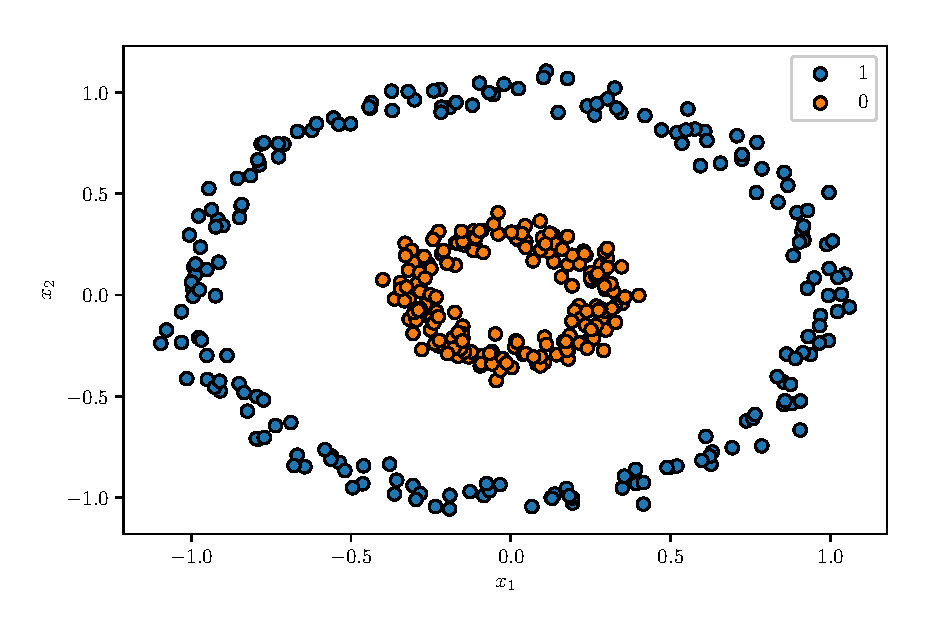
\includegraphics[width=.35\textwidth]{./gfx/input.eps}};
        %\node[inner sep=0pt] (feature) at (5,-6)
            %{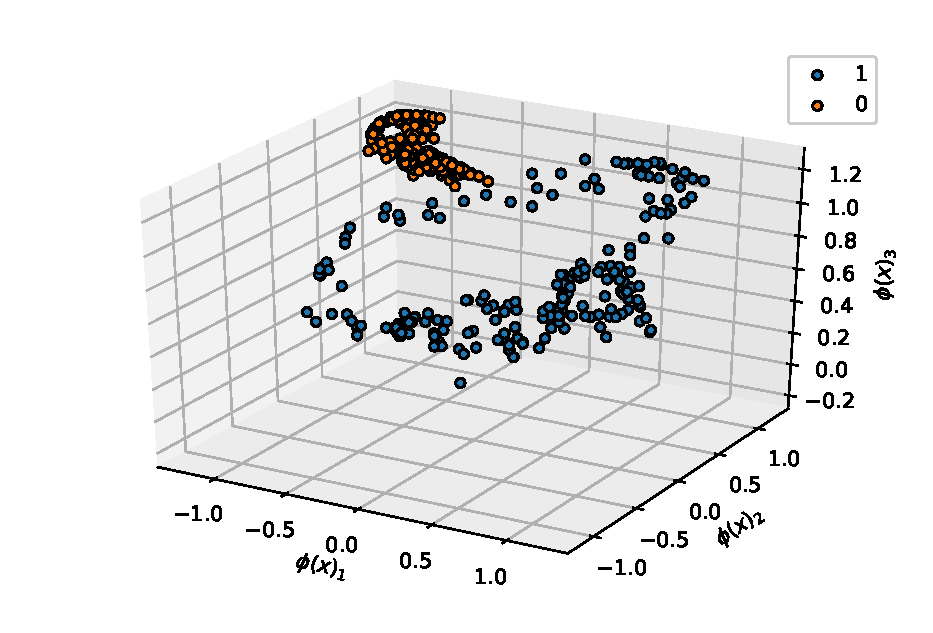
\includegraphics[width=.35\textwidth]{./gfx/feature.eps}};
        %\draw[->,thick] (input.east) -- (feature.west)
            %node[midway,fill=white] {$\phi:\mathcal{X} \to \mathcal{H}$};
    %\end{tikzpicture}}
    \centering
    \begin{tabular}{c}
        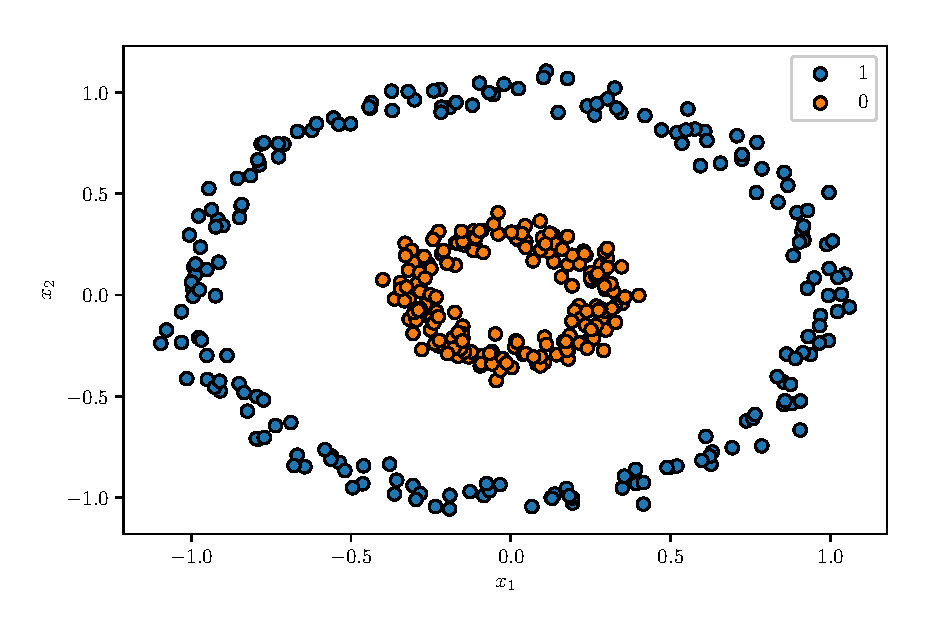
\includegraphics[valign=m, width=.5\textheight]{./gfx/input.eps} \\
        $\xdownarrow{2cm} \phi: \enskip \mathcal{X} = \mathbb{R}^2 \to
        \mathcal{H} = \mathbb{R}^3$ \\
        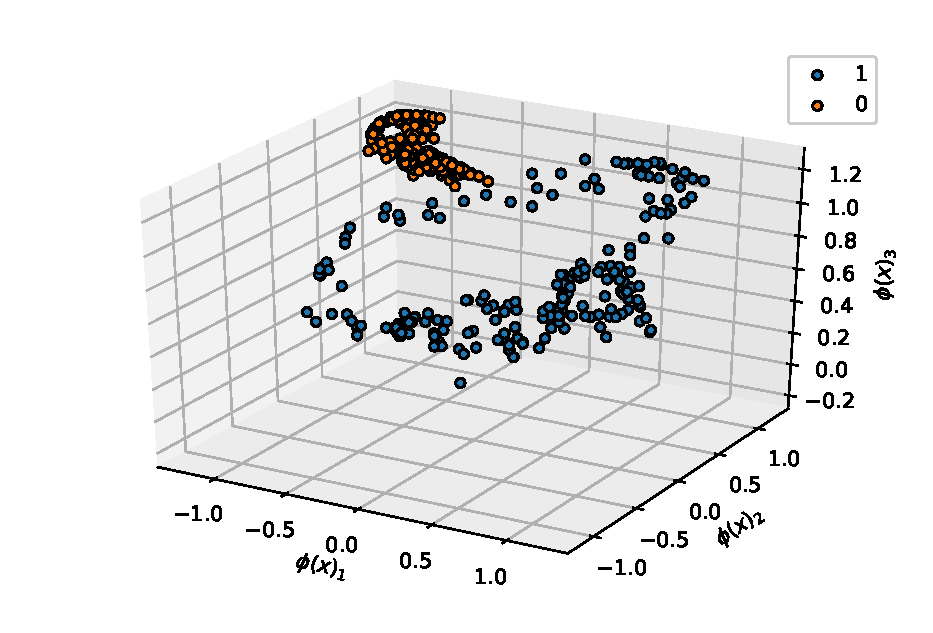
\includegraphics[valign=m, width=.5\textheight]{./gfx/feature.eps}
    \end{tabular}
    \caption[A scalar-valued feature map]{We map the two circles in
    $\mathbb{R}^2$ to $\mathbb{R}^3$. In $\mathbb{R}^3$ it is now possible to
    separate the circles with a linear functional: a plane. We used the feature
    map \\ $\phi(x) = 3.46 \begin{pmatrix} \cos(1.76 x_1 + 2.24 x_2 + 2.75) \\
    \cos(0.40 x_1 + 1.87 x_2 + 5.6) \\ \cos(0.98 x_1 - 0.98 x_2 + 6.05)
    \end{pmatrix}$. \label{fig:feature_map}}
\end{figure}
If we note
\begin{dmath*}
    \boldsymbol{\phi} =
    \begin{pmatrix}
        \phi(x_1) & \dots & \phi(x_N)
    \end{pmatrix}
\end{dmath*}
the \say{matrix} where each column represents the feature map evaluated at the
point $x_i$ with $1 \le i \le N$, the the regularized risk minimization with
the least square loss reads
\begin{dmath*}
    \mathcal{J}_{\lambda} = \frac{1}{2N}\norm{\boldsymbol{\phi}^\transpose
    \theta - (y_i)_{i=1}^N }_2^2 + \frac{\lambda}{2}\norm{\theta}_2^2.
\end{dmath*}
and the unique solution is $\theta_{\seq{s}} =
\left(\boldsymbol{\phi}\boldsymbol{\phi}^\transpose/N + \lambda
I_{\mathcal{H}}\right)^{-1}\boldsymbol{\phi} (y_i)_{i=1}^N$. This is an
$O\left( \dim(\mathcal{H})^2(N + \dim{\mathcal{H}}) \right)$. This algorithm
seems more appealing than its kernel counterpart when many data are given since
one the space $\mathcal{H}$ has been fixed, the algorithm is linear in the
number of training points. However many questions remains. First although it is
possible to design a feature map \emph{ex nihilo}, can we design systematically
a feature map from a kernel? For some kernels (\acs{eg} the gaussian kernel) it
is well known that the Hilbert space corresponding to it has dimension
$\dim(\mathcal{H}) = \infty$. Is it possible to find an approximation of the
kernel such that $\dim(\mathcal{H}) < \infty$? If such a construction is
possible and we know that $N$ data are present in the training set, is it
possible to have a sufficiently good approximation with $\dim(\mathcal{H}) \ll
N$\footnote{When $\dim(\mathcal{H}) \ge N$ then is it is better to use the
kernel algorithm than the feature algorithm. This is called the kernel trick.}?

\subsection{Random Fourier Features, Mercer Theorem, Nystr\"om method and
others}
In this subsection we answer the question whether it is possible to construct
feature maps from a given kernel, that approximate a given kernel $k$, such the
the dimension of the space $\mathcal{H} < \infty$. We start with the seminal
work of \citet{Rahimi2007} who show that given a continuous shift-invariant
kernel ($\forall x, z, t \in \mathcal{X}$, $k(x + t, z + t) = k(x, z)$), it is
possible to obtain a feature map called \acs{RFF} that approximate the given
kernel.
\subsubsection{Random Fourier Feature maps}
Random Fourier Feature methodology introduced  by Rahimi and Recht
\cite{Rahimi2007} provides a way to scale up kernel methods when kernels are
Mercer and \emph{translation-invariant}.  We view the input space $\mathcal{X}$
as a group endowed with the addition. Extensions to other group laws such as
\cite{li2010random} are described in \cref{subsubsec:skewedchi2} within the
general framework of operator-valued kernels.
\paragraph{}
Denote $k: \mathbb{R}^d \times \mathbb{R}^d \to \mathbb{R}$ a positive
definite kernel on $\mathbb{R}^d$. A kernel $k$ is said to be
\emph{shift-invariant} or \emph{translation-invariant} for the addition if for
any $a \in \mathbb{R}^d$, and for all $(x,z,t) \in \left(\mathbb{R}^d\right)^3$
we have $k(x+t,z+t) = k(x,z)$.  Then, we define $k_0: \mathbb{R}^d \to
\mathbb{R}$ the function such that $k(x,z)= k_0(x-z)$. $k_0$ is called the
\emph{signature} of kernel $k$. Bochner's theorem \cite{folland1994course} is
the theoretical result that leads to the Random Fourier Features.
\begin{theorem}[Bochner's theorem]\label{th:bochner-scalar}
    Any continuous positive definite complex function is the \acl{FT} of a
    non-negative measure.
\end{theorem}
It implies that any positive definite, continuous and shift-invariant kernel
$k$, have a continuous and positive definite signature $k_0$, which is the
\acl{FT} $\mathcal{F}$ of a non-negative measure $\mu$. We therefore have the
following corollary.
\begin{corollary}\label{c:bochner-app}
    With the previous notations and assumptions on $k$,
    \begin{dmath}\label{bochner-scalar}
        k(x,z)=k_0(x-z) \hiderel{=} \int_{\mathbb{R}^d} e^{-\iu \inner{\omega,x
        - z}} d\mu(\omega)
        =\FT{k_0}(\omega).
    \end{dmath}
\end{corollary}
Moreover $\mu = \IFT{k_0}$.  Without loss of generality, we assume that $\mu$
is a probability measure, \acs{ie} $\int_{\mathbb{R}^d} d\mu(\omega)=1$ by
renormalizing the kernel since
\begin{dmath*}
    \int_{\mathbb{R}^d}d\mu(\omega)= \int_{\mathbb{R}^d}\exp{-\iu
    \inner{\omega, 0}}d\mu(\omega)\hiderel{=}k_0(0). 
\end{dmath*}
and we can write \cref{bochner-scalar} as an expectation over $\mu$. For all
$x$,
$z\in\mathbb{R}^d$
\begin{dmath*}
    k_0(x-z) = \expectation_{\mu}\left[e^{-\iu \inner{\omega,x - z}}\right].
\end{dmath*}
Eventuallt, if $k$ is real valued we only write the real part, 
\begin{dmath*}
    k(x,z) = \expectation_{\mu}[\cos \inner{\omega,x - z}] =
    \expectation_{\mu}[ \cos \inner{\omega,z} \cos \inner{\omega,x} + \sin
    \inner{\omega,z} \sin \inner{\omega,x}].
\end{dmath*}
Let $\Vect_{j=1}^D x_j$ denote the $Dd$-length column
vector obtained by stacking vectors $x_j \in \mathbb{R}^d$.  The feature map
$\tilde{\phi}: \mathbb{R}^d \rightarrow \mathbb{R}^{2D}$ defined as
\begin{dmath}
\label{eq:rff}
    \tilde{\phi}(x)=\frac{1}{\sqrt{D}}\Vect_{j=1}^D
    \begin{pmatrix} 
        \cos{\inner{x,\omega_j}} \\
        \sin{\inner{x,\omega_j}}
    \end{pmatrix}\condition{$\omega_j \hiderel{\sim} \IFT{k_0}$ \acs{iid}}
\end{dmath}
is called a \emph{Random Fourier Feature} (map). Each $\omega_{j}, j=1, \ldots,
D$ is independently and identically sampled from the inverse Fourier transform
$\mu$ of $k_0$. This Random Fourier Feature map provides the following
Monte-Carlo estimator of the kernel: $\tilde{k}(x, z) = \tilde{\phi}(x)^*
\tilde{\phi}(z)$. Using trigonometric identities, \citet{Rahimi2007} showed
that the same feature map can also be written
\begin{dmath}
    \label{eq:rff2}
    \tilde{\phi}(x)=\frac{2}{\sqrt{D}}\Vect_{j=1}^D
    \begin{pmatrix} 
        \cos{\inner{x,\omega_j + b_j}}
    \end{pmatrix},
\end{dmath}
where $\omega_j \hiderel{\sim} \IFT{k_0}$, $b_j \sim \mathcal{U}(0, 2\pi)$
\acs{iid}.  The feature map defined by \cref{eq:rff} and \cref{eq:rff2} have
been compared in \citet{sutherland2015} where they give the condition under
wich \cref{eq:rff} has lower variance than \cref{eq:rff2}. For instance for the
gaussian kernel, \cref{eq:rff} has always lower variance. In practice,
\cref{eq:rff2} is easier to program. In this manuscript we focus on random
Fourier feature of the form \cref{eq:rff}.

\paragraph{}
The dimension $D$ governs the precision of this
approximation, whose uniform convergence towards the target kernel (as defined
in \cref{bochner-scalar}) can be found in \citet{Rahimi2007} and in more recent
papers with some refinements proposed in \citet{sutherland2015} and
\citet{sriper2015}.  Finally, it is important to notice that Random Fourier
Feature approach \emph{only} requires two steps before the application of a
learning algorithm: (1) define the inverse Fourier transform of the given
shift-invariant kernel, (2) compute the randomized feature map using the
spectral distribution $\mu$.  \citet{Rahimi2007} show that fGor the Gaussian
kernel $k_0(x-z) = \exp(-\gamma \norm{x - z}_2^2)$, the spectral distribution
$\mu$ is a Gaussian distribution. For the Laplacian kernel $k_0(x-z) =
exp(-\gamma \norm{x - z}_1)$, the spectral distribution is a Cauchy
distribution.
\paragraph{}
We now focus on another famous way of obtaining feature maps for any scalar
valued kernel called the Nystr\"om method.

\subsubsection{Nystr\"om approximation}
To overcome the bottleneck of Gram matrix computations in kernel methods,
Williams and Seeger \cite{Williams2000-nystrom} have proposed to generate a
low-rank matrix approximation of the Gram matrix using a subset of its columns.
Since this feature map is based on a decomposition of the Gram matrix, the
feature map resulting from the Nystr\"om method is data dependent. Let $k:
\mathcal{X}^2 \to \mathbb{R}$ be any scalar-valued kernel and let
\begin{dmath*}
    \seq{s} = (x_i)_{i=1}^N
\end{dmath*}
be the training data. We note a subsample fo the training data
\begin{dmath*}
    \seq{s}_M = (x_i)_{i=1}^M
\end{dmath*}
where $M \le N$ and $\seq{s}_M$ is a subsequence of $\seq{s}$. Then construct 
the gram matrix $\mathbf{K}_M$ on the subsequence $\seq{s}_M$. Namely
\begin{dmath*}
    \mathbf{K}_M =
    \begin{pmatrix}
        k(x_i, x_j)
    \end{pmatrix}_{i,j=1}^M.
\end{dmath*}
Then perform the singular-valued decomposition $\mathbf{K}_M = U \Lambda
U^\transpose$. The Nystr\"om feature map is given by
\begin{dmath*}
    \tilde{\phi}(x) = \Lambda^{-1/2} U^\transpose\left( \vect_{i=1}^M k(x, x_i)
    \right). 
\end{dmath*}
Here $M$ plays the same role than $D$ in the \acs{RFF} case: it controls the
quality of the approximation. Let $\mathbf{K}$ be the full Gram matrix on the
traing data $\seq{s}$, let 
\begin{dmath*}
    \mathbf{K}_b =
    \begin{pmatrix}
        k(x_i, x_j)
    \end{pmatrix}_{i=1, j=1}^{i=N, j=M}.
\end{dmath*}
Then it is easy to verify that $\boldsymbol{\phi}^\transpose \boldsymbol{\phi} =
\mathbf{K}_b \mathbf{K}_M^\dagger \mathbf{K}_b^\transpose \approx \mathbf{K}$,
where $\mathbf{K}_M^\dagger$ is the pseudo-inverse of $\mathbf{K}_M$ and the
quantity $\mathbf{K}_b \mathbf{K}_M^\dagger \mathbf{K}_b^\transpose$ is a low
rank approximation of the Gram matrix $\mathbf{K}$.
\paragraph{}
The main conceptual difference between the Nystr\"om features and the \acl{RFF}
is that the Nystr\"om construction is data dependent, while the \acs{RFF} is
not. The advantage of random fourier feature lies in their fast construction.
For $N$ data in $\mathbb{R}^d$, it costs $O(NDd)$ to featurize all the data.
For the Nystr\"om features it costs $O(M^2(M + d)$. Moreover if one desire to
add a new feature, the \acs{RFF} methodology is as simple as drawing a new
random vector $\omega\sim\IFT{k_0}$, compute $\cos(\inner{\omega, x} + b)$,
where $b\sim \mathcal{U}(0, 2\pi)$ and concatenate it the the existing feature.
For the Nystr\"om features one needs to recompute the singular value
decomposition of the new augmented Gram matrix $\mathbf{K}_{M+1}$.
\paragraph{}
To analyse the \acs{RFF} and Nystr\"om features authors usually study the
approximation error of the approximate Gram matrix and the targer kernel
$\norm{\boldsymbol{\phi}^\transpose\boldsymbol{\phi} - \mathbf{K}}$ (see
\citep{Yang2012, drineas2005nystrom, rosasco2010learning}) or
the supremum of the error between the approximated kernel and the true kernel
over a compact subset $\mathcal{X}$ of the support if $k$: $\sup_{(x, z)
\in\mathcal{C} \subseteq \mathcal{X}^2} \abs{\tilde{\phi}(x)^\transpose
\tilde{\phi}(z) - k(x, z)}$ (see \cite{Rahimi2007, sutherland2015, Bach2015,
rudi2016generalization}).  Because~\citet{bartlett2002rademacher} showed that
for generalization error to be below $\epsilon \in \mathbb{R}_{>0}$ for kernel
methods is $O(N^{-1/2})$, the number of samples $M$ or $D$ require to reach
somme approximation error below $\epsilon$ should be not grow faster than
$O(M^{-1/2})$ for the Nystr\"om method or $O(D^{-1/2})$ for the \acs{RFF}
method to match kernel learning.  Concerning the Nystr\"om method,
\citet{Yang2012} suggest that the number of samples $M$ is reduced to
$O(M^{-1})$ to reach an error below $\epsilon$ when the gap between the
eigenvalues of $\mathbf{K}$ is large enough. As a result in this specific case,
one should sample $M=O(\sqrt{N})$ Nystr\"om features to ensure good
generalization. On the other hand \citet{rahimi2009weighted} reported that the
generalization performance of \acs{RFF} learning is $O(N^{-1/2} + D^{-1/2})$,
which indicates that $D=O(N)$ features should be sampled to generalize well.
As a result the complexity of learning with the \acs{RFF} seems not to
deacrease. However the bounds of \citet{rahimi2009weighted} are suboptimal and
very recently (end of 2016) \citet{rudi2016generalization} proved that in the
case of ridge regression (\cref{eq:ridge_regression}), the generalization error
is $O(N^{-1/2} + D^{-1})$ meaning that $D=O(\sqrt{N})$ random features are
required for good generalization with \acsp{RFF}. We refer the interrested
reader to \citet{Yang2012} for an empirical comparison between the Nystr\"om
method and the \acs{RFF} method.


\subsubsection{Recent extensions}

\section{On large-scale learning}
\label{sec:on_large-scale_learning}

\section{History and state of the art of large scale learning with kernels}
\label{sec:history}

\chapterend
